\section{Priority Experience Replay Experiment}
The agent was trained for 10000 episodes, as detailed in section \ref{ssec:training}. The evolution of MACR100 over the 10000 episode duration is shown in Figure \ref{fig:6201_average_reward}. The highest MACR100 during training was XXXX, and the MACR100 at episode 10000 was XXXX. The trained agent performance was tested against a number of scenarios as outlined in section \ref{ssec:testing}. Training and test results are detailed in Table \ref{tab:6201_baseline_results}. Frequency and control signal plots for a +0.01pu load demand at the 15 sec mark were captured for both power system areas. Frequency plots are shown in Figures XXXX and XXXX, and control signal plots are shown in Figures XXXX and XXXX.

\vspace{2cm}

%------------------- Training Results
\begin{figure}[h]
	\centering
	% This file was created by tikzplotlib v0.9.1.
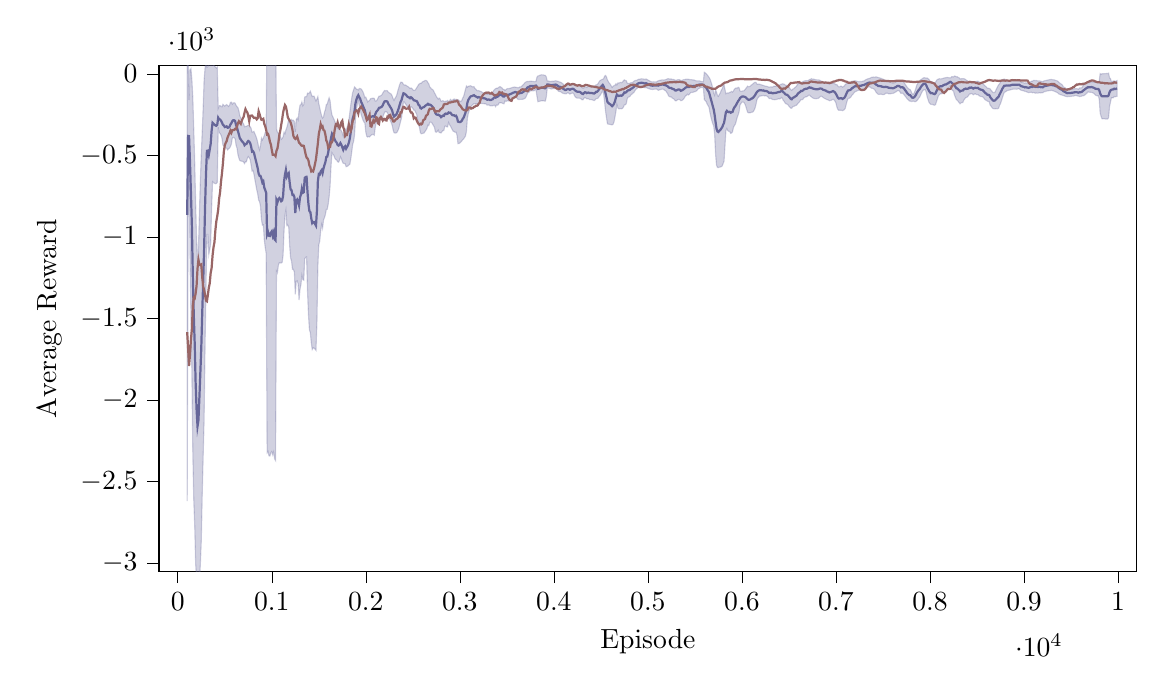
\begin{tikzpicture}

\definecolor{color0}{rgb}{1,0.498039215686275,0.0549019607843137}
\definecolor{color1}{rgb}{0.12156862745098,0.466666666666667,0.705882352941177}

\begin{axis}[
compat=newest,
tick align=outside,
tick pos=left,
x grid style={white!69.0196078431373!black},
xmin=-200.00, xmax=10200.00,
xtick style={color=black},
y grid style={white!69.0196078431373!black},
ymin=-3050.00, ymax=50.00,
ytick style={color=black},
scaled y ticks=true,
scaled y ticks=base 10:-3,
width=14cm,
height=8cm,
xlabel=Episode,
ylabel=Average Reward,
%y label style={at={(-0.2,0.5)}}
]

\path [draw=blue!20!gray, fill=blue!20!gray, opacity=0.3]
(axis cs:100,-2619.66152671753)
--(axis cs:100,892.158016068593)
--(axis cs:110,143.417432403521)
--(axis cs:120,-159.868663228158)
--(axis cs:130,24.7893742445649)
--(axis cs:140,33.333554046847)
--(axis cs:150,-33.2642814496542)
--(axis cs:160,-143.657189695485)
--(axis cs:170,-336.157031576302)
--(axis cs:180,-537.612239198292)
--(axis cs:190,-786.829676239442)
--(axis cs:200,-1012.18569074914)
--(axis cs:210,-1164.84716706992)
--(axis cs:220,-1066.52010638052)
--(axis cs:230,-853.336857007459)
--(axis cs:240,-657.089152134831)
--(axis cs:250,-493.044624742404)
--(axis cs:260,-354.251041991786)
--(axis cs:270,-207.968814158809)
--(axis cs:280,-36.041658426059)
--(axis cs:290,35.3951059587054)
--(axis cs:300,81.0433027675488)
--(axis cs:310,41.7851044334526)
--(axis cs:320,45.822575547255)
--(axis cs:330,115.543280671045)
--(axis cs:340,151.042035697885)
--(axis cs:350,184.924506173131)
--(axis cs:360,127.169113813713)
--(axis cs:370,63.8890578763668)
--(axis cs:380,57.4067109192207)
--(axis cs:390,50.6463358980554)
--(axis cs:400,42.7116077693309)
--(axis cs:410,37.0946392685346)
--(axis cs:420,42.2397167739448)
--(axis cs:430,-209.545595485802)
--(axis cs:440,-194.362869205383)
--(axis cs:450,-193.008142741514)
--(axis cs:460,-198.105684239587)
--(axis cs:470,-200.814825797196)
--(axis cs:480,-185.785044351546)
--(axis cs:490,-190.887600001776)
--(axis cs:500,-196.213660413729)
--(axis cs:510,-191.178715658053)
--(axis cs:520,-186.800473308824)
--(axis cs:530,-192.440170229498)
--(axis cs:540,-198.721705253067)
--(axis cs:550,-192.046332400587)
--(axis cs:560,-173.480616988425)
--(axis cs:570,-172.034525270181)
--(axis cs:580,-184.966025574163)
--(axis cs:590,-177.48207209218)
--(axis cs:600,-175.850621769989)
--(axis cs:610,-178.576897496839)
--(axis cs:620,-191.535040945691)
--(axis cs:630,-200.482812824836)
--(axis cs:640,-206.521766527551)
--(axis cs:650,-225.528927744388)
--(axis cs:660,-256.720712729266)
--(axis cs:670,-268.20219468699)
--(axis cs:680,-285.46056867786)
--(axis cs:690,-297.532782383731)
--(axis cs:700,-305.480136443816)
--(axis cs:710,-323.458764231164)
--(axis cs:720,-321.484351175558)
--(axis cs:730,-320.938622254352)
--(axis cs:740,-317.104020625761)
--(axis cs:750,-314.723629157764)
--(axis cs:760,-314.192825855059)
--(axis cs:770,-322.386282087952)
--(axis cs:780,-332.410424032999)
--(axis cs:790,-356.368661452699)
--(axis cs:800,-354.867942642454)
--(axis cs:810,-351.390476954994)
--(axis cs:820,-365.760643221369)
--(axis cs:830,-379.652937977043)
--(axis cs:840,-395.323525431777)
--(axis cs:850,-418.603542566595)
--(axis cs:860,-446.927768973098)
--(axis cs:870,-464.882437733692)
--(axis cs:880,-437.838875465213)
--(axis cs:890,-392.698877006504)
--(axis cs:900,-404.164732240528)
--(axis cs:910,-391.577765095429)
--(axis cs:920,-378.100482784936)
--(axis cs:930,-358.457665643661)
--(axis cs:940,-355.944545277711)
--(axis cs:950,354.704127095817)
--(axis cs:960,377.155933963715)
--(axis cs:970,357.573138550829)
--(axis cs:980,356.279106701561)
--(axis cs:990,375.005344102528)
--(axis cs:1000,385.229679860142)
--(axis cs:1010,352.65646205148)
--(axis cs:1020,373.95297769975)
--(axis cs:1030,333.286038000532)
--(axis cs:1040,329.97582236349)
--(axis cs:1050,-337.632534220744)
--(axis cs:1060,-356.644667650016)
--(axis cs:1070,-363.04632399173)
--(axis cs:1080,-363.35000298447)
--(axis cs:1090,-377.400761837185)
--(axis cs:1100,-400.938779563579)
--(axis cs:1110,-394.832134739012)
--(axis cs:1120,-385.220213337792)
--(axis cs:1130,-356.968423128672)
--(axis cs:1140,-365.745000055487)
--(axis cs:1150,-342.616415084686)
--(axis cs:1160,-327.506267741536)
--(axis cs:1170,-304.373936611007)
--(axis cs:1180,-277.579701841541)
--(axis cs:1190,-276.947049770174)
--(axis cs:1200,-287.210812936337)
--(axis cs:1210,-278.891980329164)
--(axis cs:1220,-285.335720867453)
--(axis cs:1230,-283.289014955501)
--(axis cs:1240,-291.900022041836)
--(axis cs:1250,-354.146009756239)
--(axis cs:1260,-278.642151955696)
--(axis cs:1270,-269.889973502971)
--(axis cs:1280,-281.324404314355)
--(axis cs:1290,-226.306696651361)
--(axis cs:1300,-191.134363254425)
--(axis cs:1310,-186.637121654118)
--(axis cs:1320,-171.204821332552)
--(axis cs:1330,-194.929089656005)
--(axis cs:1340,-185.292033062251)
--(axis cs:1350,-140.958121912397)
--(axis cs:1360,-138.14485614994)
--(axis cs:1370,-138.743465901711)
--(axis cs:1380,-117.037579418467)
--(axis cs:1390,-119.348802660256)
--(axis cs:1400,-114.779674183922)
--(axis cs:1410,-105.005412808382)
--(axis cs:1420,-121.939709443431)
--(axis cs:1430,-138.383617163136)
--(axis cs:1440,-135.318186096051)
--(axis cs:1450,-135.192465435235)
--(axis cs:1460,-151.909694150803)
--(axis cs:1470,-165.272413923004)
--(axis cs:1480,-153.072874370195)
--(axis cs:1490,-138.195722760184)
--(axis cs:1500,-180.328448711017)
--(axis cs:1510,-207.412123580352)
--(axis cs:1520,-233.874051807909)
--(axis cs:1530,-256.907380952397)
--(axis cs:1540,-269.644580906817)
--(axis cs:1550,-262.498722309743)
--(axis cs:1560,-234.908759080975)
--(axis cs:1570,-217.97332682647)
--(axis cs:1580,-187.025050849085)
--(axis cs:1590,-183.363956225357)
--(axis cs:1600,-162.614885702122)
--(axis cs:1610,-145.468010116827)
--(axis cs:1620,-162.338535946054)
--(axis cs:1630,-217.853338074827)
--(axis cs:1640,-250.497648983556)
--(axis cs:1650,-263.476968025274)
--(axis cs:1660,-275.836245914643)
--(axis cs:1670,-289.718697122411)
--(axis cs:1680,-304.535968552059)
--(axis cs:1690,-312.799029659845)
--(axis cs:1700,-331.776137049109)
--(axis cs:1710,-336.894900148893)
--(axis cs:1720,-338.83332699433)
--(axis cs:1730,-338.946828676747)
--(axis cs:1740,-347.749577246733)
--(axis cs:1750,-360.882730361436)
--(axis cs:1760,-381.353448880537)
--(axis cs:1770,-350.651860665683)
--(axis cs:1780,-336.66532092883)
--(axis cs:1790,-347.046930145209)
--(axis cs:1800,-328.109570835285)
--(axis cs:1810,-309.734915461839)
--(axis cs:1820,-281.631398869983)
--(axis cs:1830,-234.996290762972)
--(axis cs:1840,-188.532285077493)
--(axis cs:1850,-147.786607715002)
--(axis cs:1860,-113.981250671092)
--(axis cs:1870,-96.8355931440155)
--(axis cs:1880,-78.4892552807005)
--(axis cs:1890,-84.5225736281999)
--(axis cs:1900,-92.9212127169246)
--(axis cs:1910,-93.8106670422002)
--(axis cs:1920,-97.7369601814344)
--(axis cs:1930,-88.6032148203439)
--(axis cs:1940,-89.1270246771362)
--(axis cs:1950,-91.2702624421496)
--(axis cs:1960,-99.6431950986728)
--(axis cs:1970,-109.747016591405)
--(axis cs:1980,-124.975840452151)
--(axis cs:1990,-145.608612026297)
--(axis cs:2000,-141.708202372283)
--(axis cs:2010,-155.625330495793)
--(axis cs:2020,-170.640688805204)
--(axis cs:2030,-165.852803220698)
--(axis cs:2040,-161.148193018152)
--(axis cs:2050,-150.503155611278)
--(axis cs:2060,-150.131855068133)
--(axis cs:2070,-147.983268367726)
--(axis cs:2080,-147.383799186714)
--(axis cs:2090,-149.13059920936)
--(axis cs:2100,-165.423265004765)
--(axis cs:2110,-165.20022779846)
--(axis cs:2120,-159.228280784265)
--(axis cs:2130,-146.457132736993)
--(axis cs:2140,-135.778297887046)
--(axis cs:2150,-134.909933574662)
--(axis cs:2160,-132.010962950096)
--(axis cs:2170,-127.700741424813)
--(axis cs:2180,-116.736581312811)
--(axis cs:2190,-107.620728293087)
--(axis cs:2200,-100.471191549448)
--(axis cs:2210,-102.783781995596)
--(axis cs:2220,-100.967367083082)
--(axis cs:2230,-102.509222013596)
--(axis cs:2240,-112.121538464992)
--(axis cs:2250,-115.398812457873)
--(axis cs:2260,-119.19390610617)
--(axis cs:2270,-122.930846303379)
--(axis cs:2280,-133.49802279579)
--(axis cs:2290,-150.086552170513)
--(axis cs:2300,-161.458268487749)
--(axis cs:2310,-149.423435140194)
--(axis cs:2320,-139.734050971882)
--(axis cs:2330,-126.865946561438)
--(axis cs:2340,-103.559005234384)
--(axis cs:2350,-84.4920143081571)
--(axis cs:2360,-64.3428803505339)
--(axis cs:2370,-50.4734286590739)
--(axis cs:2380,-49.1996519060509)
--(axis cs:2390,-51.8640690255408)
--(axis cs:2400,-64.0959657896819)
--(axis cs:2410,-67.5282562512949)
--(axis cs:2420,-67.0718206516418)
--(axis cs:2430,-69.9507001797919)
--(axis cs:2440,-74.1745728595707)
--(axis cs:2450,-77.6014481677419)
--(axis cs:2460,-81.9360767910912)
--(axis cs:2470,-87.641853162809)
--(axis cs:2480,-84.9772296201055)
--(axis cs:2490,-88.3706143095472)
--(axis cs:2500,-96.7296319242037)
--(axis cs:2510,-99.8121272350313)
--(axis cs:2520,-100.388085672837)
--(axis cs:2530,-94.1740456391669)
--(axis cs:2540,-84.7995843391016)
--(axis cs:2550,-75.8353810092304)
--(axis cs:2560,-65.0986207079413)
--(axis cs:2570,-59.8944741350584)
--(axis cs:2580,-55.9146129888595)
--(axis cs:2590,-57.2847306551467)
--(axis cs:2600,-48.4551184122773)
--(axis cs:2610,-45.0113932792786)
--(axis cs:2620,-43.4957502719891)
--(axis cs:2630,-38.8901868334178)
--(axis cs:2640,-39.1642403409722)
--(axis cs:2650,-42.0087048291381)
--(axis cs:2660,-52.5897105094553)
--(axis cs:2670,-60.2929383475316)
--(axis cs:2680,-78.6148839985552)
--(axis cs:2690,-84.461534571542)
--(axis cs:2700,-91.8122723158397)
--(axis cs:2710,-94.1860239847056)
--(axis cs:2720,-101.501891234605)
--(axis cs:2730,-114.812837940954)
--(axis cs:2740,-124.369677960658)
--(axis cs:2750,-137.29490540979)
--(axis cs:2760,-146.195082160443)
--(axis cs:2770,-153.628377344503)
--(axis cs:2780,-147.137775262949)
--(axis cs:2790,-152.124400018845)
--(axis cs:2800,-167.35682964636)
--(axis cs:2810,-165.451099023495)
--(axis cs:2820,-163.277932040873)
--(axis cs:2830,-166.566581198333)
--(axis cs:2840,-170.622952909282)
--(axis cs:2850,-165.668799190569)
--(axis cs:2860,-166.495778385167)
--(axis cs:2870,-161.970961089955)
--(axis cs:2880,-173.617454856077)
--(axis cs:2890,-165.232779181777)
--(axis cs:2900,-155.441871003052)
--(axis cs:2910,-160.889034248909)
--(axis cs:2920,-161.507048387956)
--(axis cs:2930,-155.927613443131)
--(axis cs:2940,-152.735091343907)
--(axis cs:2950,-157.701953590104)
--(axis cs:2960,-154.848216422665)
--(axis cs:2970,-159.181896383476)
--(axis cs:2980,-156.386560719864)
--(axis cs:2990,-160.796982480326)
--(axis cs:3000,-166.909379369568)
--(axis cs:3010,-167.05340426563)
--(axis cs:3020,-163.252177292394)
--(axis cs:3030,-147.426476302125)
--(axis cs:3040,-137.708438371378)
--(axis cs:3050,-116.404623875368)
--(axis cs:3060,-93.6429361810282)
--(axis cs:3070,-73.3673712699593)
--(axis cs:3080,-80.2794852020606)
--(axis cs:3090,-74.2531811585503)
--(axis cs:3100,-74.2156595579071)
--(axis cs:3110,-71.4539817854838)
--(axis cs:3120,-72.8230726914501)
--(axis cs:3130,-78.0250521913816)
--(axis cs:3140,-78.1595264375167)
--(axis cs:3150,-77.0021904112291)
--(axis cs:3160,-87.8821541751977)
--(axis cs:3170,-92.2845438607121)
--(axis cs:3180,-99.7746076712901)
--(axis cs:3190,-103.102400203989)
--(axis cs:3200,-101.176247151843)
--(axis cs:3210,-104.155500423861)
--(axis cs:3220,-106.403336727915)
--(axis cs:3230,-107.906005634431)
--(axis cs:3240,-113.026638069747)
--(axis cs:3250,-115.580668994561)
--(axis cs:3260,-115.147379526974)
--(axis cs:3270,-118.540202515621)
--(axis cs:3280,-121.400791646834)
--(axis cs:3290,-124.194672272525)
--(axis cs:3300,-123.187005786357)
--(axis cs:3310,-122.9819163256)
--(axis cs:3320,-125.299932460293)
--(axis cs:3330,-123.98184555356)
--(axis cs:3340,-116.7717628811)
--(axis cs:3350,-113.627941932947)
--(axis cs:3360,-100.200355138066)
--(axis cs:3370,-95.2463889407936)
--(axis cs:3380,-89.3100162073628)
--(axis cs:3390,-86.7775474618867)
--(axis cs:3400,-86.8484859248177)
--(axis cs:3410,-83.2455865299779)
--(axis cs:3420,-78.0878495979513)
--(axis cs:3430,-77.8068963634078)
--(axis cs:3440,-81.4772185317906)
--(axis cs:3450,-85.9351943003148)
--(axis cs:3460,-93.5069590216729)
--(axis cs:3470,-94.4264826542861)
--(axis cs:3480,-100.519511918809)
--(axis cs:3490,-95.5162812809998)
--(axis cs:3500,-90.4052734406122)
--(axis cs:3510,-88.587094373984)
--(axis cs:3520,-89.3474234319558)
--(axis cs:3530,-87.8569071901336)
--(axis cs:3540,-86.3239327074194)
--(axis cs:3550,-84.2358311499127)
--(axis cs:3560,-82.4226215876358)
--(axis cs:3570,-80.3549168799665)
--(axis cs:3580,-79.5118663245157)
--(axis cs:3590,-80.4133133547494)
--(axis cs:3600,-81.4487325847821)
--(axis cs:3610,-82.5983691618592)
--(axis cs:3620,-84.2122700320515)
--(axis cs:3630,-81.5392335991048)
--(axis cs:3640,-78.3751254888106)
--(axis cs:3650,-78.6334377186492)
--(axis cs:3660,-73.8450492860034)
--(axis cs:3670,-67.9809084883458)
--(axis cs:3680,-61.7678279081983)
--(axis cs:3690,-54.3889133777194)
--(axis cs:3700,-50.1206397339623)
--(axis cs:3710,-45.9550479716405)
--(axis cs:3720,-45.4300291792869)
--(axis cs:3730,-45.9616455763772)
--(axis cs:3740,-44.7144308287315)
--(axis cs:3750,-43.0975635625884)
--(axis cs:3760,-43.5293190664401)
--(axis cs:3770,-44.6900419989531)
--(axis cs:3780,-44.89803284693)
--(axis cs:3790,-46.8381400805137)
--(axis cs:3800,-45.6822856681009)
--(axis cs:3810,-44.9658600548566)
--(axis cs:3820,-19.1651497916726)
--(axis cs:3830,-11.4719143196953)
--(axis cs:3840,-10.6057006305912)
--(axis cs:3850,-7.51070714897452)
--(axis cs:3860,-5.52487209629902)
--(axis cs:3870,-4.41828620717594)
--(axis cs:3880,-5.02941140121533)
--(axis cs:3890,-5.45480272399421)
--(axis cs:3900,-7.59492235334048)
--(axis cs:3910,-8.01886658241229)
--(axis cs:3920,-18.4965017964236)
--(axis cs:3930,-42.9273592188371)
--(axis cs:3940,-42.4073774736956)
--(axis cs:3950,-44.0990213344708)
--(axis cs:3960,-44.7129088205628)
--(axis cs:3970,-45.0743820205543)
--(axis cs:3980,-44.0881999424697)
--(axis cs:3990,-44.4247869416037)
--(axis cs:4000,-43.8229966051183)
--(axis cs:4010,-42.0031254910825)
--(axis cs:4020,-41.0424576038621)
--(axis cs:4030,-42.9133047166713)
--(axis cs:4040,-43.1250893714026)
--(axis cs:4050,-46.1859241120426)
--(axis cs:4060,-48.3241077899119)
--(axis cs:4070,-49.7089853308752)
--(axis cs:4080,-52.7922294868954)
--(axis cs:4090,-56.9609329917177)
--(axis cs:4100,-62.3781405531513)
--(axis cs:4110,-68.331771661124)
--(axis cs:4120,-73.3099504140499)
--(axis cs:4130,-72.1895595499959)
--(axis cs:4140,-69.4700913217398)
--(axis cs:4150,-67.6123903133501)
--(axis cs:4160,-67.6537605968853)
--(axis cs:4170,-69.3880383414908)
--(axis cs:4180,-67.3317179679354)
--(axis cs:4190,-64.4702250693561)
--(axis cs:4200,-63.8818779022713)
--(axis cs:4210,-63.8993535441474)
--(axis cs:4220,-60.8605231070749)
--(axis cs:4230,-62.9041997362254)
--(axis cs:4240,-66.6320704221351)
--(axis cs:4250,-68.7019440976412)
--(axis cs:4260,-69.5356405435738)
--(axis cs:4270,-69.6810009378869)
--(axis cs:4280,-73.0557726553427)
--(axis cs:4290,-78.104104868626)
--(axis cs:4300,-83.3054940015446)
--(axis cs:4310,-86.9475873951711)
--(axis cs:4320,-84.8676840635295)
--(axis cs:4330,-79.2280885200349)
--(axis cs:4340,-78.4715975581839)
--(axis cs:4350,-81.6311122113981)
--(axis cs:4360,-77.1454749488615)
--(axis cs:4370,-75.0389334875152)
--(axis cs:4380,-76.3929337902294)
--(axis cs:4390,-75.4149025787929)
--(axis cs:4400,-75.253746775539)
--(axis cs:4410,-75.5271431086851)
--(axis cs:4420,-75.6005406174395)
--(axis cs:4430,-76.7746192577376)
--(axis cs:4440,-71.8942443138972)
--(axis cs:4450,-65.7123484264105)
--(axis cs:4460,-65.6288169259693)
--(axis cs:4470,-58.6427618897622)
--(axis cs:4480,-48.601894446837)
--(axis cs:4490,-40.4997144313107)
--(axis cs:4500,-36.8458557783056)
--(axis cs:4510,-33.7671567974635)
--(axis cs:4520,-32.4178018468791)
--(axis cs:4530,-27.090705612378)
--(axis cs:4540,-12.5787890667753)
--(axis cs:4550,-8.5700821973135)
--(axis cs:4560,-18.1523101010335)
--(axis cs:4570,-36.2501234284046)
--(axis cs:4580,-46.5766663271783)
--(axis cs:4590,-56.3896033398147)
--(axis cs:4600,-62.1406727209712)
--(axis cs:4610,-72.6874406563354)
--(axis cs:4620,-82.2597760693144)
--(axis cs:4630,-74.0134880118854)
--(axis cs:4640,-70.9834999877238)
--(axis cs:4650,-69.0672146635129)
--(axis cs:4660,-59.2603760962403)
--(axis cs:4670,-66.3750311668248)
--(axis cs:4680,-54.3827324260913)
--(axis cs:4690,-54.9946834109574)
--(axis cs:4700,-53.0620435347882)
--(axis cs:4710,-50.586216915131)
--(axis cs:4720,-52.9308519966821)
--(axis cs:4730,-47.5277281797751)
--(axis cs:4740,-41.2258338228806)
--(axis cs:4750,-35.6758637478907)
--(axis cs:4760,-39.5952498695448)
--(axis cs:4770,-40.3121018145199)
--(axis cs:4780,-55.2612353006627)
--(axis cs:4790,-57.7952519365008)
--(axis cs:4800,-57.8553665542449)
--(axis cs:4810,-56.2749669220122)
--(axis cs:4820,-52.5020426704773)
--(axis cs:4830,-53.3810385415028)
--(axis cs:4840,-50.6128560824834)
--(axis cs:4850,-44.5879365996984)
--(axis cs:4860,-40.8744499167531)
--(axis cs:4870,-38.9926349316992)
--(axis cs:4880,-38.6403979327312)
--(axis cs:4890,-34.9818035543582)
--(axis cs:4900,-32.1906480730804)
--(axis cs:4910,-31.4284698557307)
--(axis cs:4920,-30.5118656074731)
--(axis cs:4930,-29.0369761342991)
--(axis cs:4940,-29.2516824971129)
--(axis cs:4950,-29.9467032915545)
--(axis cs:4960,-31.2543164539279)
--(axis cs:4970,-31.277543702928)
--(axis cs:4980,-30.0794861928414)
--(axis cs:4990,-32.374931092507)
--(axis cs:5000,-36.5848737548417)
--(axis cs:5010,-39.1511835029684)
--(axis cs:5020,-42.8970638273532)
--(axis cs:5030,-45.6742592637587)
--(axis cs:5040,-47.6655717410436)
--(axis cs:5050,-48.0147809978534)
--(axis cs:5060,-47.4863126778298)
--(axis cs:5070,-47.7626957123248)
--(axis cs:5080,-48.1403072274474)
--(axis cs:5090,-48.4928991592291)
--(axis cs:5100,-44.4777196132763)
--(axis cs:5110,-41.7412703114759)
--(axis cs:5120,-39.24390685735)
--(axis cs:5130,-38.0982808048113)
--(axis cs:5140,-36.823977114186)
--(axis cs:5150,-36.0311935172278)
--(axis cs:5160,-35.6079130890698)
--(axis cs:5170,-37.1381591790038)
--(axis cs:5180,-35.2176546494036)
--(axis cs:5190,-34.1330064927657)
--(axis cs:5200,-31.7151170931633)
--(axis cs:5210,-28.8171338395309)
--(axis cs:5220,-28.4558692027906)
--(axis cs:5230,-30.2781499534181)
--(axis cs:5240,-30.6291291842489)
--(axis cs:5250,-29.9329566436566)
--(axis cs:5260,-33.8977449212175)
--(axis cs:5270,-32.4371930272827)
--(axis cs:5280,-34.18940535633)
--(axis cs:5290,-37.4490667022053)
--(axis cs:5300,-38.2803423714583)
--(axis cs:5310,-35.6755510426799)
--(axis cs:5320,-34.4273826350923)
--(axis cs:5330,-33.8649669086944)
--(axis cs:5340,-35.2793530943946)
--(axis cs:5350,-41.5153094356863)
--(axis cs:5360,-39.1062888498427)
--(axis cs:5370,-36.6003573137939)
--(axis cs:5380,-34.356359240887)
--(axis cs:5390,-34.3092897489965)
--(axis cs:5400,-32.0036037851302)
--(axis cs:5410,-30.7630391875626)
--(axis cs:5420,-30.9075662831924)
--(axis cs:5430,-31.7710039758254)
--(axis cs:5440,-33.3146115373091)
--(axis cs:5450,-33.8291720310041)
--(axis cs:5460,-34.3523523140834)
--(axis cs:5470,-34.96330388004)
--(axis cs:5480,-36.4680222832598)
--(axis cs:5490,-35.8605268414459)
--(axis cs:5500,-38.6058249446382)
--(axis cs:5510,-41.0000380765364)
--(axis cs:5520,-41.8561443499362)
--(axis cs:5530,-41.701286566639)
--(axis cs:5540,-42.048950848713)
--(axis cs:5550,-42.1205496763296)
--(axis cs:5560,-44.4160515518196)
--(axis cs:5570,-45.4489910031665)
--(axis cs:5580,-46.5990347429145)
--(axis cs:5590,-46.9078169502624)
--(axis cs:5600,11.3674739540959)
--(axis cs:5610,7.43945131125211)
--(axis cs:5620,2.29077539040017)
--(axis cs:5630,-4.1208440652714)
--(axis cs:5640,-11.8329171019923)
--(axis cs:5650,-19.8420913952379)
--(axis cs:5660,-29.7181490797232)
--(axis cs:5670,-44.9925142571343)
--(axis cs:5680,-63.9973036638467)
--(axis cs:5690,-87.3762734235276)
--(axis cs:5700,-116.586162554918)
--(axis cs:5710,-130.038385502257)
--(axis cs:5720,-97.4230916337202)
--(axis cs:5730,-110.546552406238)
--(axis cs:5740,-131.481541903651)
--(axis cs:5750,-136.89321993115)
--(axis cs:5760,-125.227561862276)
--(axis cs:5770,-115.296371834985)
--(axis cs:5780,-100.236910456769)
--(axis cs:5790,-90.0757601298006)
--(axis cs:5800,-73.0517731840831)
--(axis cs:5810,-64.360691006646)
--(axis cs:5820,-94.5776248790465)
--(axis cs:5830,-120.808802237428)
--(axis cs:5840,-117.209979893947)
--(axis cs:5850,-115.683826093043)
--(axis cs:5860,-116.360218815207)
--(axis cs:5870,-112.19456921876)
--(axis cs:5880,-110.390930781843)
--(axis cs:5890,-106.218039335585)
--(axis cs:5900,-110.816714867101)
--(axis cs:5910,-103.138326161019)
--(axis cs:5920,-92.6265580304932)
--(axis cs:5930,-87.2576181101669)
--(axis cs:5940,-85.4562027698406)
--(axis cs:5950,-86.3262958685203)
--(axis cs:5960,-81.2181827785475)
--(axis cs:5970,-83.8518731182965)
--(axis cs:5980,-104.235987355347)
--(axis cs:5990,-104.472529728828)
--(axis cs:6000,-104.801740382402)
--(axis cs:6010,-103.024598671937)
--(axis cs:6020,-103.427042880677)
--(axis cs:6030,-97.7835758090997)
--(axis cs:6040,-89.4469973093331)
--(axis cs:6050,-82.6972883671919)
--(axis cs:6060,-74.1553144068364)
--(axis cs:6070,-77.4438700822409)
--(axis cs:6080,-76.6823895157705)
--(axis cs:6090,-73.4874522970341)
--(axis cs:6100,-66.4557514062304)
--(axis cs:6110,-64.7576734332677)
--(axis cs:6120,-58.0055838479817)
--(axis cs:6130,-53.2927264446059)
--(axis cs:6140,-50.3218207561776)
--(axis cs:6150,-51.7028006555516)
--(axis cs:6160,-62.0496052700391)
--(axis cs:6170,-62.3271975222038)
--(axis cs:6180,-61.0245094233655)
--(axis cs:6190,-62.3746876975473)
--(axis cs:6200,-64.7211603299097)
--(axis cs:6210,-66.3721372846426)
--(axis cs:6220,-68.7622575501972)
--(axis cs:6230,-69.4655625099659)
--(axis cs:6240,-72.7981439541417)
--(axis cs:6250,-74.0228188569086)
--(axis cs:6260,-74.9663003890182)
--(axis cs:6270,-76.3009299115369)
--(axis cs:6280,-79.1237322389773)
--(axis cs:6290,-80.2660113970494)
--(axis cs:6300,-78.9313484196459)
--(axis cs:6310,-78.7309744391463)
--(axis cs:6320,-79.5424826609881)
--(axis cs:6330,-78.9972695502441)
--(axis cs:6340,-74.3764986240851)
--(axis cs:6350,-74.5819082919534)
--(axis cs:6360,-74.4516012225034)
--(axis cs:6370,-72.5319738059116)
--(axis cs:6380,-70.2096984781801)
--(axis cs:6390,-68.7070592773289)
--(axis cs:6400,-67.5657022315146)
--(axis cs:6410,-63.6856583565049)
--(axis cs:6420,-61.8784025027831)
--(axis cs:6430,-59.6172466123484)
--(axis cs:6440,-60.821496265775)
--(axis cs:6450,-61.572797401413)
--(axis cs:6460,-67.9061986086515)
--(axis cs:6470,-68.6491472098738)
--(axis cs:6480,-70.7182676580167)
--(axis cs:6490,-74.4419328272566)
--(axis cs:6500,-79.1095571570417)
--(axis cs:6510,-87.9647577424751)
--(axis cs:6520,-95.9954137372618)
--(axis cs:6530,-99.7928383764271)
--(axis cs:6540,-92.5902631487244)
--(axis cs:6550,-89.8034368203925)
--(axis cs:6560,-84.7090518143899)
--(axis cs:6570,-79.7208357447425)
--(axis cs:6580,-73.9211642264261)
--(axis cs:6590,-64.8611407879527)
--(axis cs:6600,-56.9215605335776)
--(axis cs:6610,-54.9962914037673)
--(axis cs:6620,-54.8668150249606)
--(axis cs:6630,-50.1110145730034)
--(axis cs:6640,-50.8067599130082)
--(axis cs:6650,-45.411328516468)
--(axis cs:6660,-43.099884910764)
--(axis cs:6670,-41.5255638104658)
--(axis cs:6680,-40.1992636188794)
--(axis cs:6690,-40.6765234653691)
--(axis cs:6700,-40.3758737958662)
--(axis cs:6710,-37.4085620340926)
--(axis cs:6720,-33.1248385714766)
--(axis cs:6730,-32.2150104429383)
--(axis cs:6740,-28.0664383218237)
--(axis cs:6750,-31.3422990847924)
--(axis cs:6760,-30.5579242826367)
--(axis cs:6770,-32.2314147551885)
--(axis cs:6780,-34.0800979057331)
--(axis cs:6790,-35.1238529407816)
--(axis cs:6800,-35.4545408551286)
--(axis cs:6810,-35.8687381683192)
--(axis cs:6820,-35.9207653655093)
--(axis cs:6830,-38.1361728633297)
--(axis cs:6840,-42.66182782791)
--(axis cs:6850,-43.575049842559)
--(axis cs:6860,-47.9955514868994)
--(axis cs:6870,-49.2278515188295)
--(axis cs:6880,-48.8550337679102)
--(axis cs:6890,-49.503599831751)
--(axis cs:6900,-54.0277508783266)
--(axis cs:6910,-57.4232118329342)
--(axis cs:6920,-58.9256066914069)
--(axis cs:6930,-61.8383096861328)
--(axis cs:6940,-58.8902323430566)
--(axis cs:6950,-57.2681449319029)
--(axis cs:6960,-56.2585111747189)
--(axis cs:6970,-54.3632590218337)
--(axis cs:6980,-57.6820260873395)
--(axis cs:6990,-60.1366051200059)
--(axis cs:7000,-65.4511964143887)
--(axis cs:7010,-63.6739253207805)
--(axis cs:7020,-72.5615733236626)
--(axis cs:7030,-78.6752235587701)
--(axis cs:7040,-77.8181998259873)
--(axis cs:7050,-74.224536471082)
--(axis cs:7060,-73.9099597548523)
--(axis cs:7070,-80.6521472968285)
--(axis cs:7080,-76.3521849239152)
--(axis cs:7090,-72.581522938911)
--(axis cs:7100,-62.5757065941171)
--(axis cs:7110,-60.1234304095061)
--(axis cs:7120,-54.2491885352972)
--(axis cs:7130,-51.2458274728518)
--(axis cs:7140,-49.9774455079976)
--(axis cs:7150,-51.5188968995082)
--(axis cs:7160,-47.9031994126003)
--(axis cs:7170,-43.9802812521826)
--(axis cs:7180,-43.9863370228379)
--(axis cs:7190,-42.2964813347751)
--(axis cs:7200,-40.6849923475599)
--(axis cs:7210,-41.6699558337051)
--(axis cs:7220,-43.8392974198847)
--(axis cs:7230,-45.1328686920385)
--(axis cs:7240,-46.5554424290616)
--(axis cs:7250,-45.8575981419838)
--(axis cs:7260,-45.7931173007236)
--(axis cs:7270,-46.2331996127068)
--(axis cs:7280,-44.2050752209341)
--(axis cs:7290,-42.7951561385783)
--(axis cs:7300,-42.3843101118873)
--(axis cs:7310,-37.0858915770401)
--(axis cs:7320,-33.8609230191213)
--(axis cs:7330,-31.3936763688731)
--(axis cs:7340,-28.9371432826886)
--(axis cs:7350,-27.5033498410645)
--(axis cs:7360,-25.740223554198)
--(axis cs:7370,-22.6778179636826)
--(axis cs:7380,-19.8624243149262)
--(axis cs:7390,-18.9853166457466)
--(axis cs:7400,-18.2035749996181)
--(axis cs:7410,-18.9998334152507)
--(axis cs:7420,-17.9578386163544)
--(axis cs:7430,-17.4332283333291)
--(axis cs:7440,-19.1130682933255)
--(axis cs:7450,-21.6431957707253)
--(axis cs:7460,-22.6838706526523)
--(axis cs:7470,-24.4795763555923)
--(axis cs:7480,-26.2678347835863)
--(axis cs:7490,-29.3369164084154)
--(axis cs:7500,-30.6543162878315)
--(axis cs:7510,-33.8971933962292)
--(axis cs:7520,-36.5342286327728)
--(axis cs:7530,-38.5149557587377)
--(axis cs:7540,-40.941213353625)
--(axis cs:7550,-44.2106173906215)
--(axis cs:7560,-47.07664566793)
--(axis cs:7570,-48.1150367383017)
--(axis cs:7580,-50.0312798047839)
--(axis cs:7590,-51.6746881696317)
--(axis cs:7600,-54.8933189575976)
--(axis cs:7610,-54.944685238878)
--(axis cs:7620,-54.3170812407142)
--(axis cs:7630,-51.6424127621798)
--(axis cs:7640,-48.0926474510077)
--(axis cs:7650,-44.6952069903691)
--(axis cs:7660,-44.2515288988134)
--(axis cs:7670,-44.6190460617528)
--(axis cs:7680,-45.7720641248883)
--(axis cs:7690,-45.7171452248441)
--(axis cs:7700,-44.8236700697807)
--(axis cs:7710,-45.1263487617905)
--(axis cs:7720,-48.0566288519994)
--(axis cs:7730,-56.1951922234527)
--(axis cs:7740,-65.2453217967367)
--(axis cs:7750,-73.9946861630543)
--(axis cs:7760,-82.6386765016668)
--(axis cs:7770,-88.8298104490217)
--(axis cs:7780,-92.9686226234284)
--(axis cs:7790,-94.8575937666805)
--(axis cs:7800,-105.812544337043)
--(axis cs:7810,-119.822809281345)
--(axis cs:7820,-125.165628555341)
--(axis cs:7830,-118.462302439581)
--(axis cs:7840,-104.432746056757)
--(axis cs:7850,-86.9717428295653)
--(axis cs:7860,-67.7100935377904)
--(axis cs:7870,-56.8677142897321)
--(axis cs:7880,-48.5466359023212)
--(axis cs:7890,-43.0621357623663)
--(axis cs:7900,-35.5610920428242)
--(axis cs:7910,-31.3534444529368)
--(axis cs:7920,-28.7402230537337)
--(axis cs:7930,-23.3084075988199)
--(axis cs:7940,-22.4796094868884)
--(axis cs:7950,-23.5919207857193)
--(axis cs:7960,-24.9562698566518)
--(axis cs:7970,-23.7263616628575)
--(axis cs:7980,-28.1969809826928)
--(axis cs:7990,-32.9729396675162)
--(axis cs:8000,-42.3878513760512)
--(axis cs:8010,-48.2206222989739)
--(axis cs:8020,-46.3378050862988)
--(axis cs:8030,-50.835028045087)
--(axis cs:8040,-52.1490663161898)
--(axis cs:8050,-54.5317533442243)
--(axis cs:8060,-49.3737726589916)
--(axis cs:8070,-39.1351718084239)
--(axis cs:8080,-32.7898235856986)
--(axis cs:8090,-31.2903820126097)
--(axis cs:8100,-28.2872610832984)
--(axis cs:8110,-29.6263132054888)
--(axis cs:8120,-29.7307249344825)
--(axis cs:8130,-27.9497338384704)
--(axis cs:8140,-26.6271157218487)
--(axis cs:8150,-24.2451140838294)
--(axis cs:8160,-22.9241475885888)
--(axis cs:8170,-22.3371553655287)
--(axis cs:8180,-20.5757544534251)
--(axis cs:8190,-21.1306073948985)
--(axis cs:8200,-22.3616227847309)
--(axis cs:8210,-22.9898022084293)
--(axis cs:8220,-23.4738392637023)
--(axis cs:8230,-15.9465560971924)
--(axis cs:8240,-16.4307930944467)
--(axis cs:8250,-17.8851880675658)
--(axis cs:8260,-12.0203859030423)
--(axis cs:8270,-12.8175649955248)
--(axis cs:8280,-16.9873462876867)
--(axis cs:8290,-16.2183595130396)
--(axis cs:8300,-20.3752231777654)
--(axis cs:8310,-22.8910721329748)
--(axis cs:8320,-30.4479572154545)
--(axis cs:8330,-28.4025558142759)
--(axis cs:8340,-28.6245451199991)
--(axis cs:8350,-27.8951998024921)
--(axis cs:8360,-28.04863428484)
--(axis cs:8370,-30.287096811963)
--(axis cs:8380,-33.799145080323)
--(axis cs:8390,-39.1178309909946)
--(axis cs:8400,-40.6032163061858)
--(axis cs:8410,-45.5867609732565)
--(axis cs:8420,-43.754407873583)
--(axis cs:8430,-46.3927883553938)
--(axis cs:8440,-45.1069836293207)
--(axis cs:8450,-48.2032995502506)
--(axis cs:8460,-50.3755177975239)
--(axis cs:8470,-48.6429575495933)
--(axis cs:8480,-47.303368797019)
--(axis cs:8490,-45.9969921494016)
--(axis cs:8500,-44.4255997977747)
--(axis cs:8510,-43.2925508490905)
--(axis cs:8520,-47.5675300591358)
--(axis cs:8530,-49.9888198539337)
--(axis cs:8540,-53.7635798539181)
--(axis cs:8550,-54.4802939451967)
--(axis cs:8560,-58.2308096330024)
--(axis cs:8570,-63.5867661429196)
--(axis cs:8580,-68.5390295095859)
--(axis cs:8590,-74.7711065038284)
--(axis cs:8600,-79.1711564961188)
--(axis cs:8610,-86.6936109480254)
--(axis cs:8620,-86.2249371425455)
--(axis cs:8630,-87.7871536297098)
--(axis cs:8640,-90.71814316108)
--(axis cs:8650,-99.7072741660076)
--(axis cs:8660,-105.302051158007)
--(axis cs:8670,-112.365816722262)
--(axis cs:8680,-114.095922933994)
--(axis cs:8690,-112.483298569196)
--(axis cs:8700,-100.502128355288)
--(axis cs:8710,-88.0559431835676)
--(axis cs:8720,-76.0962545177651)
--(axis cs:8730,-66.4822659101636)
--(axis cs:8740,-59.5001300696289)
--(axis cs:8750,-47.8716238882978)
--(axis cs:8760,-39.9698781872171)
--(axis cs:8770,-34.1014089369513)
--(axis cs:8780,-32.5864394118201)
--(axis cs:8790,-30.2770164027653)
--(axis cs:8800,-33.1583583140851)
--(axis cs:8810,-34.2001910602585)
--(axis cs:8820,-40.179134770129)
--(axis cs:8830,-41.161151205492)
--(axis cs:8840,-41.5338321636723)
--(axis cs:8850,-43.9226309439905)
--(axis cs:8860,-40.2319453536436)
--(axis cs:8870,-39.1654936174812)
--(axis cs:8880,-37.8432547386105)
--(axis cs:8890,-38.4844592418957)
--(axis cs:8900,-37.8805891770781)
--(axis cs:8910,-38.787598955178)
--(axis cs:8920,-38.7191715730003)
--(axis cs:8930,-39.2263590915843)
--(axis cs:8940,-39.3976876881197)
--(axis cs:8950,-39.20716033703)
--(axis cs:8960,-44.4767867998461)
--(axis cs:8970,-49.8575782299721)
--(axis cs:8980,-50.4080477788284)
--(axis cs:8990,-53.1172628334293)
--(axis cs:9000,-53.6300818981211)
--(axis cs:9010,-56.1655528577435)
--(axis cs:9020,-53.23904425834)
--(axis cs:9030,-55.1218866036621)
--(axis cs:9040,-54.4800458504968)
--(axis cs:9050,-55.1206477622112)
--(axis cs:9060,-52.1219607124748)
--(axis cs:9070,-47.672831063395)
--(axis cs:9080,-43.7506296677808)
--(axis cs:9090,-43.857915248916)
--(axis cs:9100,-39.5267258351901)
--(axis cs:9110,-38.4622179786657)
--(axis cs:9120,-40.5572043073821)
--(axis cs:9130,-39.2200650725392)
--(axis cs:9140,-41.2597034001558)
--(axis cs:9150,-41.9454941318824)
--(axis cs:9160,-41.7387301743369)
--(axis cs:9170,-42.379609130774)
--(axis cs:9180,-45.6907488944963)
--(axis cs:9190,-44.5785682576875)
--(axis cs:9200,-47.4847209079756)
--(axis cs:9210,-42.816496061995)
--(axis cs:9220,-40.798625805438)
--(axis cs:9230,-40.1956812933269)
--(axis cs:9240,-38.5015516593697)
--(axis cs:9250,-37.1101812679772)
--(axis cs:9260,-35.9907823639611)
--(axis cs:9270,-34.2825740636263)
--(axis cs:9280,-33.72617685925)
--(axis cs:9290,-32.6140176468359)
--(axis cs:9300,-34.1591849116745)
--(axis cs:9310,-35.4051109221991)
--(axis cs:9320,-35.0833086835328)
--(axis cs:9330,-37.5073320946643)
--(axis cs:9340,-39.8120345859844)
--(axis cs:9350,-40.6056287795334)
--(axis cs:9360,-44.2105859559723)
--(axis cs:9370,-50.2434416645262)
--(axis cs:9380,-54.7874891535299)
--(axis cs:9390,-59.4588139933356)
--(axis cs:9400,-62.6261017150086)
--(axis cs:9410,-68.9441353694532)
--(axis cs:9420,-78.7163429620187)
--(axis cs:9430,-81.8759638802372)
--(axis cs:9440,-84.5171003171548)
--(axis cs:9450,-91.538509834928)
--(axis cs:9460,-95.4310121327487)
--(axis cs:9470,-95.6387055830659)
--(axis cs:9480,-95.3141919583495)
--(axis cs:9490,-95.6696705657787)
--(axis cs:9500,-93.7381805719776)
--(axis cs:9510,-93.3079057365726)
--(axis cs:9520,-92.1554246790138)
--(axis cs:9530,-91.1766503880009)
--(axis cs:9540,-90.2655571265822)
--(axis cs:9550,-89.577348924546)
--(axis cs:9560,-89.2390424999841)
--(axis cs:9570,-91.2037049425938)
--(axis cs:9580,-93.1247809857851)
--(axis cs:9590,-85.6608573438648)
--(axis cs:9600,-84.880156768508)
--(axis cs:9610,-85.088981238127)
--(axis cs:9620,-80.1292830253265)
--(axis cs:9630,-68.7324151348698)
--(axis cs:9640,-62.9372889684169)
--(axis cs:9650,-58.4444292703489)
--(axis cs:9660,-54.5689605989404)
--(axis cs:9670,-51.8674845120386)
--(axis cs:9680,-50.5028755265811)
--(axis cs:9690,-53.2086017528443)
--(axis cs:9700,-51.0180213706743)
--(axis cs:9710,-49.1165701119555)
--(axis cs:9720,-46.5049158005714)
--(axis cs:9730,-48.6572305079127)
--(axis cs:9740,-49.4738252112489)
--(axis cs:9750,-50.1158538848515)
--(axis cs:9760,-50.8663983763724)
--(axis cs:9770,-49.8790201916481)
--(axis cs:9780,-49.6317981946569)
--(axis cs:9790,-48.8575781544638)
--(axis cs:9800,-43.3795368348157)
--(axis cs:9810,2.61259005870085)
--(axis cs:9820,-2.46528887633804)
--(axis cs:9830,2.43264856545633)
--(axis cs:9840,1.26314913207034)
--(axis cs:9850,2.57433608071386)
--(axis cs:9860,2.210524203766)
--(axis cs:9870,2.5409336726529)
--(axis cs:9880,3.76115809405945)
--(axis cs:9890,2.9684545975181)
--(axis cs:9900,5.84665866816454)
--(axis cs:9910,-23.2855025456712)
--(axis cs:9920,-27.4033987734754)
--(axis cs:9930,-47.1222262263852)
--(axis cs:9940,-43.6910009425569)
--(axis cs:9950,-42.7530589342959)
--(axis cs:9960,-41.7443241140493)
--(axis cs:9970,-44.1525978441019)
--(axis cs:9980,-42.585132783356)
--(axis cs:9990,-40.0121724267366)
--(axis cs:9990,-136.63026694349)
--(axis cs:9990,-136.63026694349)
--(axis cs:9980,-137.467111955305)
--(axis cs:9970,-139.388895948745)
--(axis cs:9960,-137.603069376263)
--(axis cs:9950,-145.425835914348)
--(axis cs:9940,-145.444146374408)
--(axis cs:9930,-145.371544426079)
--(axis cs:9920,-172.487633375382)
--(axis cs:9910,-199.405795814118)
--(axis cs:9900,-267.945917062263)
--(axis cs:9890,-275.617810793918)
--(axis cs:9880,-275.261800707277)
--(axis cs:9870,-275.557267082339)
--(axis cs:9860,-275.220079099738)
--(axis cs:9850,-273.369679388449)
--(axis cs:9840,-274.496041354827)
--(axis cs:9830,-274.215059061074)
--(axis cs:9820,-259.614655661966)
--(axis cs:9810,-238.710101490223)
--(axis cs:9800,-152.490612008303)
--(axis cs:9790,-133.364135054982)
--(axis cs:9780,-133.529690254247)
--(axis cs:9770,-131.755138128915)
--(axis cs:9760,-129.262299490668)
--(axis cs:9750,-122.59290305123)
--(axis cs:9740,-117.096220855316)
--(axis cs:9730,-115.034391487318)
--(axis cs:9720,-112.057109097701)
--(axis cs:9710,-111.859219223471)
--(axis cs:9700,-111.579895320282)
--(axis cs:9690,-110.305041690072)
--(axis cs:9680,-110.262933176144)
--(axis cs:9670,-116.284848717677)
--(axis cs:9660,-122.042831991717)
--(axis cs:9650,-126.781364548628)
--(axis cs:9640,-131.363587414949)
--(axis cs:9630,-133.745899461374)
--(axis cs:9620,-133.65798697213)
--(axis cs:9610,-136.412860366432)
--(axis cs:9600,-137.260329967206)
--(axis cs:9590,-138.041385749146)
--(axis cs:9580,-135.010309649817)
--(axis cs:9570,-134.643656093019)
--(axis cs:9560,-132.238841918399)
--(axis cs:9550,-131.94654034103)
--(axis cs:9540,-132.0691259711)
--(axis cs:9530,-134.821488836141)
--(axis cs:9520,-135.658640130289)
--(axis cs:9510,-135.660411663947)
--(axis cs:9500,-137.520423627525)
--(axis cs:9490,-137.097143513097)
--(axis cs:9480,-138.32657560371)
--(axis cs:9470,-137.151775667192)
--(axis cs:9460,-138.809312867392)
--(axis cs:9450,-137.471477908385)
--(axis cs:9440,-137.175134657723)
--(axis cs:9430,-133.294831201869)
--(axis cs:9420,-132.32293722409)
--(axis cs:9410,-130.593429078811)
--(axis cs:9400,-128.275660506503)
--(axis cs:9390,-126.747162507866)
--(axis cs:9380,-123.857661646653)
--(axis cs:9370,-122.062379276256)
--(axis cs:9360,-115.72947411996)
--(axis cs:9350,-111.950840691861)
--(axis cs:9340,-109.704787849067)
--(axis cs:9330,-107.521122561576)
--(axis cs:9320,-104.478637943064)
--(axis cs:9310,-103.152666811586)
--(axis cs:9300,-101.20442015374)
--(axis cs:9290,-99.4391168912454)
--(axis cs:9280,-101.2202737709)
--(axis cs:9270,-101.307725583111)
--(axis cs:9260,-103.012916471266)
--(axis cs:9250,-103.213456942184)
--(axis cs:9240,-104.741835207427)
--(axis cs:9230,-106.800134221315)
--(axis cs:9220,-106.600074694119)
--(axis cs:9210,-110.167038659257)
--(axis cs:9200,-114.69680441006)
--(axis cs:9190,-113.687229495652)
--(axis cs:9180,-116.364318172928)
--(axis cs:9170,-114.33240605214)
--(axis cs:9160,-115.196641563537)
--(axis cs:9150,-116.824465062581)
--(axis cs:9140,-117.188269437847)
--(axis cs:9130,-115.473746931427)
--(axis cs:9120,-117.544847515753)
--(axis cs:9110,-114.056111980367)
--(axis cs:9100,-113.150331565473)
--(axis cs:9090,-114.77793175605)
--(axis cs:9080,-111.441695448117)
--(axis cs:9070,-112.115593289641)
--(axis cs:9060,-112.481465361558)
--(axis cs:9050,-114.171655986675)
--(axis cs:9040,-111.82606778591)
--(axis cs:9030,-110.033372779746)
--(axis cs:9020,-106.452461270356)
--(axis cs:9010,-106.894126468705)
--(axis cs:9000,-103.507608158058)
--(axis cs:8990,-102.344826706145)
--(axis cs:8980,-100.616553938721)
--(axis cs:8970,-99.5117844108206)
--(axis cs:8960,-96.1454332009759)
--(axis cs:8950,-90.4283259627072)
--(axis cs:8940,-90.3277317773802)
--(axis cs:8930,-92.1256477153782)
--(axis cs:8920,-93.0854020449756)
--(axis cs:8910,-92.5255480481541)
--(axis cs:8900,-92.1086109528261)
--(axis cs:8890,-92.6410304781716)
--(axis cs:8880,-93.0184240956819)
--(axis cs:8870,-93.9208419412713)
--(axis cs:8860,-96.7425593038704)
--(axis cs:8850,-97.6704791234488)
--(axis cs:8840,-98.9853237913252)
--(axis cs:8830,-100.232717797884)
--(axis cs:8820,-101.727948992343)
--(axis cs:8810,-106.149582604247)
--(axis cs:8800,-110.170966126735)
--(axis cs:8790,-112.437887920557)
--(axis cs:8780,-128.607196863613)
--(axis cs:8770,-145.862594693354)
--(axis cs:8760,-164.680094623249)
--(axis cs:8750,-182.058519193992)
--(axis cs:8740,-192.098562308372)
--(axis cs:8730,-210.454616452347)
--(axis cs:8720,-212.672470121259)
--(axis cs:8710,-212.183651155063)
--(axis cs:8700,-213.248818047603)
--(axis cs:8690,-212.418549220049)
--(axis cs:8680,-212.92729318061)
--(axis cs:8670,-211.520264723394)
--(axis cs:8660,-205.392758034636)
--(axis cs:8650,-196.490248149672)
--(axis cs:8640,-190.787603697928)
--(axis cs:8630,-169.74736887543)
--(axis cs:8620,-167.838017441803)
--(axis cs:8610,-166.192010102625)
--(axis cs:8600,-161.334775594869)
--(axis cs:8590,-159.22357968914)
--(axis cs:8580,-153.289569142659)
--(axis cs:8570,-144.023250350945)
--(axis cs:8560,-139.241414703032)
--(axis cs:8550,-138.202603164024)
--(axis cs:8540,-137.47231389892)
--(axis cs:8530,-135.605648299874)
--(axis cs:8520,-131.999277626971)
--(axis cs:8510,-125.633152586949)
--(axis cs:8500,-126.636453079246)
--(axis cs:8490,-124.154874434095)
--(axis cs:8480,-120.63967640649)
--(axis cs:8470,-123.797300613718)
--(axis cs:8460,-127.467487857663)
--(axis cs:8450,-121.69427312685)
--(axis cs:8440,-118.730544172808)
--(axis cs:8430,-122.053841570872)
--(axis cs:8420,-122.616722177697)
--(axis cs:8410,-131.807405768244)
--(axis cs:8400,-139.117028579734)
--(axis cs:8390,-143.314816907716)
--(axis cs:8380,-144.161606745072)
--(axis cs:8370,-152.883513226124)
--(axis cs:8360,-159.328113315007)
--(axis cs:8350,-174.431338859503)
--(axis cs:8340,-174.736339337639)
--(axis cs:8330,-177.053967380671)
--(axis cs:8320,-182.414141833034)
--(axis cs:8310,-175.447141388603)
--(axis cs:8300,-167.376301921706)
--(axis cs:8290,-160.437208509293)
--(axis cs:8280,-156.409129580025)
--(axis cs:8270,-141.415343667074)
--(axis cs:8260,-127.629022827465)
--(axis cs:8250,-104.081152090684)
--(axis cs:8240,-101.222406180775)
--(axis cs:8230,-90.1284453785676)
--(axis cs:8220,-71.6745000514941)
--(axis cs:8210,-74.6671529078223)
--(axis cs:8200,-84.3537499230131)
--(axis cs:8190,-93.1680439586849)
--(axis cs:8180,-100.252789681568)
--(axis cs:8170,-105.067927056794)
--(axis cs:8160,-105.710580623421)
--(axis cs:8150,-108.972323730997)
--(axis cs:8140,-112.509216390803)
--(axis cs:8130,-120.393569451788)
--(axis cs:8120,-121.506392980324)
--(axis cs:8110,-120.748493057144)
--(axis cs:8100,-127.18768796324)
--(axis cs:8090,-132.652983806891)
--(axis cs:8080,-151.899330466869)
--(axis cs:8070,-168.59690424121)
--(axis cs:8060,-186.719375034595)
--(axis cs:8050,-191.17364583354)
--(axis cs:8040,-190.307152732214)
--(axis cs:8030,-186.76537175043)
--(axis cs:8020,-186.397905723168)
--(axis cs:8010,-186.362407115426)
--(axis cs:8000,-180.706012284385)
--(axis cs:7990,-174.071491240819)
--(axis cs:7980,-156.937570297069)
--(axis cs:7970,-139.271639686898)
--(axis cs:7960,-110.678347058026)
--(axis cs:7950,-95.7578089185204)
--(axis cs:7940,-95.5734799472029)
--(axis cs:7930,-98.9920575912078)
--(axis cs:7920,-105.767963413786)
--(axis cs:7910,-116.092206596588)
--(axis cs:7900,-129.3608476582)
--(axis cs:7890,-141.837029026004)
--(axis cs:7880,-147.872914428816)
--(axis cs:7870,-157.332628185128)
--(axis cs:7860,-163.608973046774)
--(axis cs:7850,-168.806495689816)
--(axis cs:7840,-169.607372097822)
--(axis cs:7830,-167.295169128442)
--(axis cs:7820,-165.767021523625)
--(axis cs:7810,-168.196762033627)
--(axis cs:7800,-168.138632406524)
--(axis cs:7790,-165.239287323952)
--(axis cs:7780,-165.256555532292)
--(axis cs:7770,-158.250054374662)
--(axis cs:7760,-154.024470625462)
--(axis cs:7750,-145.809209078384)
--(axis cs:7740,-138.223423768755)
--(axis cs:7730,-130.868352622796)
--(axis cs:7720,-124.055222871745)
--(axis cs:7710,-117.362925670853)
--(axis cs:7700,-117.426435698228)
--(axis cs:7690,-117.822950741599)
--(axis cs:7680,-107.675119326173)
--(axis cs:7670,-102.151626319638)
--(axis cs:7660,-100.430882809199)
--(axis cs:7650,-103.823566890643)
--(axis cs:7640,-109.095935362201)
--(axis cs:7630,-110.864351829495)
--(axis cs:7620,-114.978097944785)
--(axis cs:7610,-118.430045970227)
--(axis cs:7600,-118.90562541043)
--(axis cs:7590,-119.499517119775)
--(axis cs:7580,-121.207680558293)
--(axis cs:7570,-121.078359229967)
--(axis cs:7560,-121.198514555332)
--(axis cs:7550,-117.362052164225)
--(axis cs:7540,-117.648810927708)
--(axis cs:7530,-117.730145204318)
--(axis cs:7520,-122.883608156429)
--(axis cs:7510,-126.052552269944)
--(axis cs:7500,-126.066225388266)
--(axis cs:7490,-125.372609269645)
--(axis cs:7480,-122.75748174938)
--(axis cs:7470,-123.996578182941)
--(axis cs:7460,-124.286639586339)
--(axis cs:7450,-124.699900746465)
--(axis cs:7440,-118.022533101525)
--(axis cs:7430,-114.120733348258)
--(axis cs:7420,-103.942371900946)
--(axis cs:7410,-94.4137401059452)
--(axis cs:7400,-90.4435502963223)
--(axis cs:7390,-87.259080164001)
--(axis cs:7380,-87.5968756525282)
--(axis cs:7370,-83.4205642262765)
--(axis cs:7360,-78.1998459129153)
--(axis cs:7350,-78.5096485961801)
--(axis cs:7340,-80.4390955851869)
--(axis cs:7330,-83.39203975704)
--(axis cs:7320,-86.2043333259226)
--(axis cs:7310,-89.2225773334448)
--(axis cs:7300,-91.7102955969486)
--(axis cs:7290,-92.5707465287144)
--(axis cs:7280,-93.0472010411592)
--(axis cs:7270,-96.148368198717)
--(axis cs:7260,-97.7246424809226)
--(axis cs:7250,-98.7226190577836)
--(axis cs:7240,-99.7523607418616)
--(axis cs:7230,-100.926405022242)
--(axis cs:7220,-105.165932196531)
--(axis cs:7210,-107.042860478623)
--(axis cs:7200,-110.132722320746)
--(axis cs:7190,-116.394155594386)
--(axis cs:7180,-124.877395450315)
--(axis cs:7170,-129.830900798512)
--(axis cs:7160,-140.353748690646)
--(axis cs:7150,-145.457514335239)
--(axis cs:7140,-149.079558125336)
--(axis cs:7130,-149.620524968888)
--(axis cs:7120,-163.594599942707)
--(axis cs:7110,-184.432285071013)
--(axis cs:7100,-209.041878458334)
--(axis cs:7090,-218.151674465195)
--(axis cs:7080,-221.984947505243)
--(axis cs:7070,-224.536998170003)
--(axis cs:7060,-222.16505342457)
--(axis cs:7050,-222.146106090585)
--(axis cs:7040,-221.689428019062)
--(axis cs:7030,-222.227329419702)
--(axis cs:7020,-216.440640156087)
--(axis cs:7010,-201.833161576452)
--(axis cs:7000,-177.409480024068)
--(axis cs:6990,-165.641688964733)
--(axis cs:6980,-158.687996610347)
--(axis cs:6970,-154.368776467342)
--(axis cs:6960,-157.621737991663)
--(axis cs:6950,-160.987645080862)
--(axis cs:6940,-162.151921423572)
--(axis cs:6930,-163.841418129935)
--(axis cs:6920,-159.071667161524)
--(axis cs:6910,-157.912604152687)
--(axis cs:6900,-155.940301197209)
--(axis cs:6890,-152.059964443272)
--(axis cs:6880,-150.00484624142)
--(axis cs:6870,-146.208370387934)
--(axis cs:6860,-141.995159902423)
--(axis cs:6850,-136.837986598487)
--(axis cs:6840,-135.548323608063)
--(axis cs:6830,-139.714566153582)
--(axis cs:6820,-146.247885518629)
--(axis cs:6810,-149.989583463625)
--(axis cs:6800,-149.157239101179)
--(axis cs:6790,-151.513574386694)
--(axis cs:6780,-150.6054561388)
--(axis cs:6770,-150.137031966545)
--(axis cs:6760,-148.392731071546)
--(axis cs:6750,-144.839264609922)
--(axis cs:6740,-139.954421270338)
--(axis cs:6730,-136.594157722662)
--(axis cs:6720,-129.612753708893)
--(axis cs:6710,-129.921787891345)
--(axis cs:6700,-134.966886408555)
--(axis cs:6690,-138.909464418926)
--(axis cs:6680,-139.467759496792)
--(axis cs:6670,-142.533596179991)
--(axis cs:6660,-145.392083637625)
--(axis cs:6650,-153.959445972543)
--(axis cs:6640,-157.643927386964)
--(axis cs:6630,-155.978863014558)
--(axis cs:6620,-163.798377358914)
--(axis cs:6610,-171.912944566066)
--(axis cs:6600,-177.75442565001)
--(axis cs:6590,-184.506408752343)
--(axis cs:6580,-192.106311639583)
--(axis cs:6570,-192.721426537982)
--(axis cs:6560,-196.424284100541)
--(axis cs:6550,-198.318690580147)
--(axis cs:6540,-201.106961646441)
--(axis cs:6530,-209.449751054499)
--(axis cs:6520,-209.556753231399)
--(axis cs:6510,-203.28772184133)
--(axis cs:6500,-197.035689251266)
--(axis cs:6490,-188.966585968097)
--(axis cs:6480,-184.164339241382)
--(axis cs:6470,-182.917599936638)
--(axis cs:6460,-178.020460585706)
--(axis cs:6450,-167.641073459246)
--(axis cs:6440,-162.351779369676)
--(axis cs:6430,-147.745124828579)
--(axis cs:6420,-143.460651115481)
--(axis cs:6410,-150.873715971808)
--(axis cs:6400,-152.793001001687)
--(axis cs:6390,-151.126452863076)
--(axis cs:6380,-153.611020161067)
--(axis cs:6370,-155.543659453109)
--(axis cs:6360,-156.354480947408)
--(axis cs:6350,-157.754910698584)
--(axis cs:6340,-156.709713033263)
--(axis cs:6330,-157.12883702423)
--(axis cs:6320,-154.438021847251)
--(axis cs:6310,-148.478517120274)
--(axis cs:6300,-149.824286723743)
--(axis cs:6290,-150.631704728144)
--(axis cs:6280,-141.863585267475)
--(axis cs:6270,-136.822854372933)
--(axis cs:6260,-134.023428104938)
--(axis cs:6250,-133.20141529303)
--(axis cs:6240,-134.495565682187)
--(axis cs:6230,-130.72288594608)
--(axis cs:6220,-132.425252726793)
--(axis cs:6210,-133.392785147064)
--(axis cs:6200,-135.043881300578)
--(axis cs:6190,-134.293821357644)
--(axis cs:6180,-140.179855076439)
--(axis cs:6170,-146.232249704692)
--(axis cs:6160,-157.467849197138)
--(axis cs:6150,-186.17902657152)
--(axis cs:6140,-208.520280132044)
--(axis cs:6130,-221.983986176319)
--(axis cs:6120,-231.076013065893)
--(axis cs:6110,-234.094971207266)
--(axis cs:6100,-234.378638176563)
--(axis cs:6090,-237.588053013298)
--(axis cs:6080,-237.491105091499)
--(axis cs:6070,-238.131716542592)
--(axis cs:6060,-233.662100853962)
--(axis cs:6050,-215.106630736268)
--(axis cs:6040,-195.380166040857)
--(axis cs:6030,-181.924842641011)
--(axis cs:6020,-173.194364967517)
--(axis cs:6010,-171.682912453995)
--(axis cs:6000,-172.163054400047)
--(axis cs:5990,-180.572179628754)
--(axis cs:5980,-189.978417671074)
--(axis cs:5970,-231.760565184079)
--(axis cs:5960,-250.934402457076)
--(axis cs:5950,-265.817318311237)
--(axis cs:5940,-288.543923936031)
--(axis cs:5930,-307.672197163742)
--(axis cs:5920,-315.878472061661)
--(axis cs:5910,-327.410814224456)
--(axis cs:5900,-354.719313434198)
--(axis cs:5890,-361.66568017228)
--(axis cs:5880,-363.888368062519)
--(axis cs:5870,-351.382530072158)
--(axis cs:5860,-350.890126975194)
--(axis cs:5850,-347.765446389624)
--(axis cs:5840,-334.021194529649)
--(axis cs:5830,-346.599419418824)
--(axis cs:5820,-439.925716433166)
--(axis cs:5810,-534.495349932554)
--(axis cs:5800,-549.284711239278)
--(axis cs:5790,-564.189862622977)
--(axis cs:5780,-567.98744459849)
--(axis cs:5770,-570.645667232366)
--(axis cs:5760,-570.716378587686)
--(axis cs:5750,-573.617194160392)
--(axis cs:5740,-572.839382284665)
--(axis cs:5730,-559.231106511294)
--(axis cs:5720,-492.010285012516)
--(axis cs:5710,-370.398138364677)
--(axis cs:5700,-318.329940388468)
--(axis cs:5690,-305.065668028475)
--(axis cs:5680,-285.476156274182)
--(axis cs:5670,-262.268305653305)
--(axis cs:5660,-236.098517330498)
--(axis cs:5650,-203.315898137246)
--(axis cs:5640,-193.510837676173)
--(axis cs:5630,-182.982246197377)
--(axis cs:5620,-169.712628902829)
--(axis cs:5610,-162.332706331276)
--(axis cs:5600,-156.725912206347)
--(axis cs:5590,-83.0273288134566)
--(axis cs:5580,-83.2456435761878)
--(axis cs:5570,-82.615003646651)
--(axis cs:5560,-83.0666346360939)
--(axis cs:5550,-87.156388464096)
--(axis cs:5540,-89.2962629070594)
--(axis cs:5530,-93.6016857050368)
--(axis cs:5520,-102.652695327398)
--(axis cs:5510,-105.676736911163)
--(axis cs:5500,-108.783281593803)
--(axis cs:5490,-108.910122037192)
--(axis cs:5480,-111.660590766486)
--(axis cs:5470,-113.334689591074)
--(axis cs:5460,-112.185821860419)
--(axis cs:5450,-117.34820288161)
--(axis cs:5440,-125.080914609026)
--(axis cs:5430,-128.274461434553)
--(axis cs:5420,-123.668499087087)
--(axis cs:5410,-131.165672884311)
--(axis cs:5400,-134.205316918475)
--(axis cs:5390,-144.083150516217)
--(axis cs:5380,-152.720555530762)
--(axis cs:5370,-158.355107560868)
--(axis cs:5360,-162.408565727242)
--(axis cs:5350,-163.481278624038)
--(axis cs:5340,-157.387219423941)
--(axis cs:5330,-154.900695247281)
--(axis cs:5320,-156.586164912252)
--(axis cs:5310,-159.91952746358)
--(axis cs:5300,-164.463846897853)
--(axis cs:5290,-163.42676830283)
--(axis cs:5280,-154.537667068458)
--(axis cs:5270,-150.291478540195)
--(axis cs:5260,-147.887415600202)
--(axis cs:5250,-140.904099594235)
--(axis cs:5240,-140.555758968385)
--(axis cs:5230,-137.928289975606)
--(axis cs:5220,-134.299389415972)
--(axis cs:5210,-120.145499400001)
--(axis cs:5200,-112.503190217712)
--(axis cs:5190,-102.417404067655)
--(axis cs:5180,-100.749138703494)
--(axis cs:5170,-95.3802157811958)
--(axis cs:5160,-92.3025620467362)
--(axis cs:5150,-92.6360019475668)
--(axis cs:5140,-94.2417655280286)
--(axis cs:5130,-95.5010132105517)
--(axis cs:5120,-97.8927687921735)
--(axis cs:5110,-99.9539455329805)
--(axis cs:5100,-94.3456179154238)
--(axis cs:5090,-91.5041730948859)
--(axis cs:5080,-92.4021402466007)
--(axis cs:5070,-92.5769412159932)
--(axis cs:5060,-93.7305962274887)
--(axis cs:5050,-94.7712539291895)
--(axis cs:5040,-93.6895058635295)
--(axis cs:5030,-93.3617214687718)
--(axis cs:5020,-91.483346426087)
--(axis cs:5010,-89.1173184031553)
--(axis cs:5000,-87.9487464852309)
--(axis cs:4990,-84.7933149955611)
--(axis cs:4980,-82.5874774209652)
--(axis cs:4970,-83.8136244655242)
--(axis cs:4960,-82.4229578832094)
--(axis cs:4950,-79.666751939147)
--(axis cs:4940,-78.3436469136263)
--(axis cs:4930,-77.0992548167285)
--(axis cs:4920,-78.1363603545379)
--(axis cs:4910,-78.7507216847812)
--(axis cs:4900,-80.585452020161)
--(axis cs:4890,-85.6203003751909)
--(axis cs:4880,-90.9175170468932)
--(axis cs:4870,-95.8134191595531)
--(axis cs:4860,-104.332768138267)
--(axis cs:4850,-114.461400935049)
--(axis cs:4840,-116.781391982569)
--(axis cs:4830,-123.151194008745)
--(axis cs:4820,-127.935729508265)
--(axis cs:4810,-136.256156949621)
--(axis cs:4800,-140.270955424002)
--(axis cs:4790,-141.946531297111)
--(axis cs:4780,-153.175715138836)
--(axis cs:4770,-181.860726287586)
--(axis cs:4760,-188.196573566028)
--(axis cs:4750,-189.478293721368)
--(axis cs:4740,-201.78225736955)
--(axis cs:4730,-211.176036177398)
--(axis cs:4720,-213.101740393631)
--(axis cs:4710,-211.782412052732)
--(axis cs:4700,-213.387799416925)
--(axis cs:4690,-213.460374195556)
--(axis cs:4680,-207.66882691199)
--(axis cs:4670,-185.043420113771)
--(axis cs:4660,-229.461592344057)
--(axis cs:4650,-263.070940422975)
--(axis cs:4640,-292.934275453436)
--(axis cs:4630,-307.951688925606)
--(axis cs:4620,-311.737213035753)
--(axis cs:4610,-310.797543809248)
--(axis cs:4600,-309.026733369745)
--(axis cs:4590,-308.121685348255)
--(axis cs:4580,-307.319005733449)
--(axis cs:4570,-305.281191509836)
--(axis cs:4560,-269.118783807061)
--(axis cs:4550,-230.20438862318)
--(axis cs:4540,-175.095121497021)
--(axis cs:4530,-124.964005525457)
--(axis cs:4520,-101.437912281685)
--(axis cs:4510,-110.947175280135)
--(axis cs:4500,-122.516501784651)
--(axis cs:4490,-133.116621491252)
--(axis cs:4480,-139.051777079396)
--(axis cs:4470,-147.271585173185)
--(axis cs:4460,-150.965408075493)
--(axis cs:4450,-150.854394055847)
--(axis cs:4440,-157.785744413537)
--(axis cs:4430,-162.320403339954)
--(axis cs:4420,-161.446856182184)
--(axis cs:4410,-158.821333591585)
--(axis cs:4400,-156.272934792216)
--(axis cs:4390,-157.034184178963)
--(axis cs:4380,-156.718958844481)
--(axis cs:4370,-152.057145742532)
--(axis cs:4360,-151.32137444732)
--(axis cs:4350,-151.829911111041)
--(axis cs:4340,-146.775192916998)
--(axis cs:4330,-143.311242829611)
--(axis cs:4320,-148.402175120094)
--(axis cs:4310,-158.512681230786)
--(axis cs:4300,-158.17458885302)
--(axis cs:4290,-152.189147321678)
--(axis cs:4280,-148.910785736104)
--(axis cs:4270,-147.436691258722)
--(axis cs:4260,-147.203530355853)
--(axis cs:4250,-147.887200242247)
--(axis cs:4240,-145.830748236072)
--(axis cs:4230,-141.268235702528)
--(axis cs:4220,-133.55808124635)
--(axis cs:4210,-118.946698787108)
--(axis cs:4200,-116.175594395129)
--(axis cs:4190,-117.838081798221)
--(axis cs:4180,-119.974372987333)
--(axis cs:4170,-122.756321255451)
--(axis cs:4160,-118.269006701121)
--(axis cs:4150,-114.985089811067)
--(axis cs:4140,-117.051652140664)
--(axis cs:4130,-121.821569288861)
--(axis cs:4120,-121.729157788894)
--(axis cs:4110,-119.472106124346)
--(axis cs:4100,-118.819224853597)
--(axis cs:4090,-116.03830759219)
--(axis cs:4080,-112.078737224141)
--(axis cs:4070,-107.34760670605)
--(axis cs:4060,-107.746483299707)
--(axis cs:4050,-106.076308443231)
--(axis cs:4040,-99.6332483146455)
--(axis cs:4030,-91.6585010155358)
--(axis cs:4020,-87.9120115196711)
--(axis cs:4010,-88.8722166552005)
--(axis cs:4000,-88.4816813718928)
--(axis cs:3990,-89.3881752789225)
--(axis cs:3980,-90.7660956998847)
--(axis cs:3970,-91.7412689578452)
--(axis cs:3960,-88.685731458911)
--(axis cs:3950,-87.0976368895495)
--(axis cs:3940,-86.4679839967141)
--(axis cs:3930,-84.772887838336)
--(axis cs:3920,-138.793779250429)
--(axis cs:3910,-165.50353235447)
--(axis cs:3900,-165.388220095669)
--(axis cs:3890,-164.131756229427)
--(axis cs:3880,-163.738253794285)
--(axis cs:3870,-163.970126456194)
--(axis cs:3860,-164.960411977851)
--(axis cs:3850,-166.676081718016)
--(axis cs:3840,-168.311821595794)
--(axis cs:3830,-169.572806328101)
--(axis cs:3820,-135.617876383358)
--(axis cs:3810,-95.9474169692184)
--(axis cs:3800,-98.2289925993574)
--(axis cs:3790,-102.514149495947)
--(axis cs:3780,-102.294381963737)
--(axis cs:3770,-102.172286796423)
--(axis cs:3760,-102.121846649002)
--(axis cs:3750,-102.324745702263)
--(axis cs:3740,-110.175398961372)
--(axis cs:3730,-111.751533446581)
--(axis cs:3720,-118.018246873695)
--(axis cs:3710,-132.252175027651)
--(axis cs:3700,-144.072706250458)
--(axis cs:3690,-150.071669341146)
--(axis cs:3680,-152.769905473105)
--(axis cs:3670,-154.552042515686)
--(axis cs:3660,-154.858091624856)
--(axis cs:3650,-155.251929784921)
--(axis cs:3640,-154.916574426906)
--(axis cs:3630,-156.255688553699)
--(axis cs:3620,-155.445408328865)
--(axis cs:3610,-149.543911981605)
--(axis cs:3600,-142.1346697761)
--(axis cs:3590,-139.111678399776)
--(axis cs:3580,-144.995479193012)
--(axis cs:3570,-147.670974597733)
--(axis cs:3560,-150.689959308178)
--(axis cs:3550,-155.593741474563)
--(axis cs:3540,-157.900537607458)
--(axis cs:3530,-160.579298352666)
--(axis cs:3520,-165.225976366406)
--(axis cs:3510,-164.049822851679)
--(axis cs:3500,-164.958096668744)
--(axis cs:3490,-168.193835478456)
--(axis cs:3480,-164.643621672541)
--(axis cs:3470,-182.051469799577)
--(axis cs:3460,-181.593528327328)
--(axis cs:3450,-178.16171876368)
--(axis cs:3440,-176.215920961274)
--(axis cs:3430,-176.108380147481)
--(axis cs:3420,-175.555819923181)
--(axis cs:3410,-187.720471931336)
--(axis cs:3400,-190.978063895884)
--(axis cs:3390,-190.007294178551)
--(axis cs:3380,-200.267164353786)
--(axis cs:3370,-190.637396879824)
--(axis cs:3360,-192.059827465166)
--(axis cs:3350,-195.115868482606)
--(axis cs:3340,-195.512388412021)
--(axis cs:3330,-194.435838032302)
--(axis cs:3320,-194.166097503531)
--(axis cs:3310,-189.421125478932)
--(axis cs:3300,-190.511113616548)
--(axis cs:3290,-190.375336592917)
--(axis cs:3280,-184.366711000206)
--(axis cs:3270,-182.153264224118)
--(axis cs:3260,-182.536880328922)
--(axis cs:3250,-180.900576702558)
--(axis cs:3240,-181.114226562673)
--(axis cs:3230,-180.354970582104)
--(axis cs:3220,-179.658452103692)
--(axis cs:3210,-182.176361289861)
--(axis cs:3200,-180.803418909163)
--(axis cs:3190,-184.993027538338)
--(axis cs:3180,-181.623648453577)
--(axis cs:3170,-182.675346944452)
--(axis cs:3160,-181.861220111322)
--(axis cs:3150,-182.100470241986)
--(axis cs:3140,-185.530095229304)
--(axis cs:3130,-192.263657504671)
--(axis cs:3120,-198.955001359853)
--(axis cs:3110,-208.288867092485)
--(axis cs:3100,-224.878755529809)
--(axis cs:3090,-242.704486030125)
--(axis cs:3080,-272.763211994892)
--(axis cs:3070,-351.872426893366)
--(axis cs:3060,-380.878630257497)
--(axis cs:3050,-388.943033276956)
--(axis cs:3040,-398.484879212917)
--(axis cs:3030,-402.292840765931)
--(axis cs:3020,-411.783824702535)
--(axis cs:3010,-417.216411241079)
--(axis cs:3000,-422.723385298493)
--(axis cs:2990,-426.535060583746)
--(axis cs:2980,-426.987299992219)
--(axis cs:2970,-375.875544249693)
--(axis cs:2960,-356.133177674171)
--(axis cs:2950,-357.408975159607)
--(axis cs:2940,-353.450071544267)
--(axis cs:2930,-351.011633867707)
--(axis cs:2920,-341.638273852134)
--(axis cs:2910,-329.677199650917)
--(axis cs:2900,-318.274307671302)
--(axis cs:2890,-310.345698834907)
--(axis cs:2880,-297.118774384367)
--(axis cs:2870,-324.44988419769)
--(axis cs:2860,-323.675729579883)
--(axis cs:2850,-318.854026671322)
--(axis cs:2840,-319.851322421685)
--(axis cs:2830,-346.02836788822)
--(axis cs:2820,-346.49030251725)
--(axis cs:2810,-353.649435897605)
--(axis cs:2800,-361.405077907661)
--(axis cs:2790,-359.169245497871)
--(axis cs:2780,-358.771061932706)
--(axis cs:2770,-344.063119077672)
--(axis cs:2760,-352.623317604328)
--(axis cs:2750,-356.929562696101)
--(axis cs:2740,-355.164540180179)
--(axis cs:2730,-326.719966367352)
--(axis cs:2720,-316.417498338053)
--(axis cs:2710,-307.261041319982)
--(axis cs:2700,-297.05786421842)
--(axis cs:2690,-294.929405313871)
--(axis cs:2680,-294.763331635287)
--(axis cs:2670,-316.374037956681)
--(axis cs:2660,-313.343927426537)
--(axis cs:2650,-334.448424082749)
--(axis cs:2640,-344.101454557398)
--(axis cs:2630,-351.99898049634)
--(axis cs:2620,-361.363380271424)
--(axis cs:2610,-362.7467893934)
--(axis cs:2600,-364.660213006524)
--(axis cs:2590,-366.403193840127)
--(axis cs:2580,-359.641744089021)
--(axis cs:2570,-324.994179310682)
--(axis cs:2560,-311.590615670624)
--(axis cs:2550,-270.921496221993)
--(axis cs:2540,-244.99930750641)
--(axis cs:2530,-235.002735264528)
--(axis cs:2520,-222.276822233339)
--(axis cs:2510,-221.401690519557)
--(axis cs:2500,-210.699486086044)
--(axis cs:2490,-202.983148151649)
--(axis cs:2480,-200.525277791752)
--(axis cs:2470,-208.837021478076)
--(axis cs:2460,-205.504119237933)
--(axis cs:2450,-203.769023645839)
--(axis cs:2440,-200.718461995114)
--(axis cs:2430,-188.694883465151)
--(axis cs:2420,-181.536201445852)
--(axis cs:2410,-171.55401253396)
--(axis cs:2400,-171.435049844882)
--(axis cs:2390,-222.070909236209)
--(axis cs:2380,-269.048030043643)
--(axis cs:2370,-290.543337408363)
--(axis cs:2360,-313.669201614822)
--(axis cs:2350,-334.580991000522)
--(axis cs:2340,-348.414770939746)
--(axis cs:2330,-358.291846327469)
--(axis cs:2320,-361.274023607097)
--(axis cs:2310,-361.825239043158)
--(axis cs:2300,-359.723202116724)
--(axis cs:2290,-341.493387552271)
--(axis cs:2280,-313.581438253413)
--(axis cs:2270,-298.360454082814)
--(axis cs:2260,-285.170397305349)
--(axis cs:2250,-267.70601588628)
--(axis cs:2240,-255.84301752303)
--(axis cs:2230,-236.7157713565)
--(axis cs:2220,-231.275638719631)
--(axis cs:2210,-229.46496449975)
--(axis cs:2200,-234.857270832537)
--(axis cs:2190,-247.97049856525)
--(axis cs:2180,-267.008658900637)
--(axis cs:2170,-272.714749832809)
--(axis cs:2160,-275.492205288946)
--(axis cs:2150,-277.009844585858)
--(axis cs:2140,-279.08368623021)
--(axis cs:2130,-291.116580167885)
--(axis cs:2120,-292.217894072227)
--(axis cs:2110,-300.936439964254)
--(axis cs:2100,-328.903216176722)
--(axis cs:2090,-375.008770485382)
--(axis cs:2080,-370.194635447149)
--(axis cs:2070,-370.702771086028)
--(axis cs:2060,-373.825041567727)
--(axis cs:2050,-377.952356380092)
--(axis cs:2040,-385.597438492059)
--(axis cs:2030,-382.646135061525)
--(axis cs:2020,-386.515221658968)
--(axis cs:2010,-381.509094936479)
--(axis cs:2000,-357.594038903699)
--(axis cs:1990,-300.696135565684)
--(axis cs:1980,-294.871563081771)
--(axis cs:1970,-282.44179231715)
--(axis cs:1960,-265.401931163547)
--(axis cs:1950,-248.304007908644)
--(axis cs:1940,-213.878894799771)
--(axis cs:1930,-194.220338846081)
--(axis cs:1920,-161.013523624302)
--(axis cs:1910,-186.571779220231)
--(axis cs:1900,-219.902108901798)
--(axis cs:1890,-274.552971615818)
--(axis cs:1880,-374.300572025017)
--(axis cs:1870,-413.984058798548)
--(axis cs:1860,-432.330612638632)
--(axis cs:1850,-478.775491384638)
--(axis cs:1840,-521.729252238477)
--(axis cs:1830,-554.365201352774)
--(axis cs:1820,-557.395177756839)
--(axis cs:1810,-563.662985073021)
--(axis cs:1800,-566.488973067773)
--(axis cs:1790,-568.38717332591)
--(axis cs:1780,-549.593588618856)
--(axis cs:1770,-548.628667337956)
--(axis cs:1760,-547.834941772498)
--(axis cs:1750,-537.509618868429)
--(axis cs:1740,-519.31826946105)
--(axis cs:1730,-507.756431527013)
--(axis cs:1720,-529.904023381948)
--(axis cs:1710,-540.850962269519)
--(axis cs:1700,-538.156860806504)
--(axis cs:1690,-527.633932517888)
--(axis cs:1680,-524.392585125246)
--(axis cs:1670,-515.843439955584)
--(axis cs:1660,-498.678387118018)
--(axis cs:1650,-492.515145028122)
--(axis cs:1640,-482.762143990182)
--(axis cs:1630,-564.88253281886)
--(axis cs:1620,-685.492382545337)
--(axis cs:1610,-753.23194484489)
--(axis cs:1600,-797.934341862528)
--(axis cs:1590,-829.049700926315)
--(axis cs:1580,-829.943576085754)
--(axis cs:1570,-862.124602854845)
--(axis cs:1560,-881.177049967917)
--(axis cs:1550,-895.041692977842)
--(axis cs:1540,-946.534284246592)
--(axis cs:1530,-922.629253860063)
--(axis cs:1520,-961.636387596695)
--(axis cs:1510,-1025.50926997179)
--(axis cs:1500,-1046.73447420787)
--(axis cs:1490,-1177.94098963237)
--(axis cs:1480,-1525.70473429429)
--(axis cs:1470,-1694.47845499436)
--(axis cs:1460,-1687.12878782633)
--(axis cs:1450,-1680.81401286632)
--(axis cs:1440,-1678.68870525633)
--(axis cs:1430,-1689.73716216087)
--(axis cs:1420,-1648.12645716227)
--(axis cs:1410,-1587.03153459708)
--(axis cs:1400,-1568.40883963235)
--(axis cs:1390,-1476.04345089644)
--(axis cs:1380,-1334.90729491912)
--(axis cs:1370,-1121.84598197119)
--(axis cs:1360,-1124.11930406255)
--(axis cs:1350,-1133.41629367753)
--(axis cs:1340,-1264.61643647465)
--(axis cs:1330,-1261.56141941453)
--(axis cs:1320,-1234.97967392314)
--(axis cs:1310,-1290.99799719138)
--(axis cs:1300,-1320.84093193456)
--(axis cs:1290,-1385.96557826268)
--(axis cs:1280,-1286.22170582489)
--(axis cs:1270,-1268.43126968498)
--(axis cs:1260,-1272.70131021718)
--(axis cs:1250,-1351.69963897766)
--(axis cs:1240,-1215.01655604493)
--(axis cs:1230,-1197.37924484704)
--(axis cs:1220,-1197.63192534017)
--(axis cs:1210,-1147.45821919123)
--(axis cs:1200,-1127.4227365419)
--(axis cs:1190,-1052.59128627499)
--(axis cs:1180,-938.481600480995)
--(axis cs:1170,-926.489638732168)
--(axis cs:1160,-929.607917948636)
--(axis cs:1150,-834.072048369245)
--(axis cs:1140,-867.3549196357)
--(axis cs:1130,-964.621149843903)
--(axis cs:1120,-1111.7773021039)
--(axis cs:1110,-1155.47764769487)
--(axis cs:1100,-1158.7772933842)
--(axis cs:1090,-1158.56743148698)
--(axis cs:1080,-1157.35511441279)
--(axis cs:1070,-1172.42742848448)
--(axis cs:1060,-1219.09395276418)
--(axis cs:1050,-1209.13250901347)
--(axis cs:1040,-2370.74345098256)
--(axis cs:1030,-2361.09483696959)
--(axis cs:1020,-2317.5857780123)
--(axis cs:1010,-2336.03262338781)
--(axis cs:1000,-2315.27325983721)
--(axis cs:990,-2322.66047433056)
--(axis cs:980,-2343.10055867123)
--(axis cs:970,-2341.51244478584)
--(axis cs:960,-2314.92885688198)
--(axis cs:950,-2322.86908021328)
--(axis cs:940,-1100.47139915688)
--(axis cs:930,-1063.26517709356)
--(axis cs:920,-1015.71680702658)
--(axis cs:910,-924.994146333188)
--(axis cs:900,-927.120259332865)
--(axis cs:890,-892.171645150618)
--(axis cs:880,-812.282526268908)
--(axis cs:870,-783.080546217291)
--(axis cs:860,-773.050094238894)
--(axis cs:850,-735.309260437353)
--(axis cs:840,-709.955963230339)
--(axis cs:830,-678.574552077791)
--(axis cs:820,-646.904679075695)
--(axis cs:810,-613.361352163937)
--(axis cs:800,-590.977722574106)
--(axis cs:790,-594.907168133606)
--(axis cs:780,-556.700685196503)
--(axis cs:770,-523.688474848517)
--(axis cs:760,-514.393505837589)
--(axis cs:750,-506.301393392578)
--(axis cs:740,-516.457608902403)
--(axis cs:730,-538.177138271838)
--(axis cs:720,-538.041256433794)
--(axis cs:710,-549.04612614723)
--(axis cs:700,-539.496984815542)
--(axis cs:690,-535.324747051155)
--(axis cs:680,-534.585373425354)
--(axis cs:670,-532.857815984133)
--(axis cs:660,-530.731474739987)
--(axis cs:650,-515.6266583701)
--(axis cs:640,-493.736732043294)
--(axis cs:630,-454.213809997307)
--(axis cs:620,-436.108479246966)
--(axis cs:610,-397.035667420594)
--(axis cs:600,-391.036873647189)
--(axis cs:590,-388.344309294733)
--(axis cs:580,-392.560676228523)
--(axis cs:570,-429.94227257741)
--(axis cs:560,-444.844011702363)
--(axis cs:550,-454.76642395789)
--(axis cs:540,-458.539324975888)
--(axis cs:530,-465.686749776431)
--(axis cs:520,-454.688892500049)
--(axis cs:510,-454.597793821195)
--(axis cs:500,-453.746397162205)
--(axis cs:490,-440.662418520688)
--(axis cs:480,-436.110492619602)
--(axis cs:470,-393.129430610314)
--(axis cs:460,-374.804432519477)
--(axis cs:450,-364.178017918148)
--(axis cs:440,-359.683309338999)
--(axis cs:430,-325.635336578455)
--(axis cs:420,-664.247506673709)
--(axis cs:410,-671.898904110287)
--(axis cs:400,-672.597947820535)
--(axis cs:390,-669.604084741545)
--(axis cs:380,-664.986917249668)
--(axis cs:370,-659.962860079709)
--(axis cs:360,-822.527058288374)
--(axis cs:350,-1040.2918156377)
--(axis cs:340,-1077.08319417281)
--(axis cs:330,-1107.48623433063)
--(axis cs:320,-984.1620811621)
--(axis cs:310,-983.66512588769)
--(axis cs:300,-1312.33123757504)
--(axis cs:290,-1672.4458939392)
--(axis cs:280,-2123.15183076347)
--(axis cs:270,-2346.98665299394)
--(axis cs:260,-2583.17846959916)
--(axis cs:250,-2865.47359517956)
--(axis cs:240,-3009.80872149497)
--(axis cs:230,-3114.35441745601)
--(axis cs:220,-3178.33951593896)
--(axis cs:210,-3156.40189967882)
--(axis cs:200,-3099.6889793513)
--(axis cs:190,-3002.42458979869)
--(axis cs:180,-2767.29559927141)
--(axis cs:170,-2610.61899381168)
--(axis cs:160,-2325.81394746227)
--(axis cs:150,-1827.24638621221)
--(axis cs:140,-1491.61472088202)
--(axis cs:130,-1108.32177933884)
--(axis cs:120,-601.789006216664)
--(axis cs:110,-902.826538676062)
--(axis cs:100,-2619.66152671753)
--cycle;

\addplot [thick, blue!20!gray]
table {%
100 -863.751755324467
110 -379.70455313627
120 -380.828834722411
130 -541.766202547139
140 -729.140583417585
150 -930.255333830933
160 -1234.73556857888
170 -1473.38801269399
180 -1652.45391923485
190 -1894.62713301906
200 -2055.93733505022
210 -2160.62453337437
220 -2122.42981115974
230 -1983.84563723173
240 -1833.4489368149
250 -1679.25910996098
260 -1468.71475579547
270 -1277.47773357638
280 -1079.59674459476
290 -818.525393990245
300 -615.643967403747
310 -470.940010727119
320 -469.169752807423
330 -495.97147682979
340 -463.020579237462
350 -427.683654732286
360 -347.67897223733
370 -298.036901101671
380 -303.790103165224
390 -309.478874421745
400 -314.943170025602
410 -317.402132420876
420 -311.003894949882
430 -267.590466032129
440 -277.023089272191
450 -278.593080329831
460 -286.455058379532
470 -296.972128203755
480 -310.947768485574
490 -315.775009261232
500 -324.980028787967
510 -322.888254739624
520 -320.744682904437
530 -329.063460002964
540 -328.630515114478
550 -323.406378179239
560 -309.162314345394
570 -300.988398923796
580 -288.763350901343
590 -282.913190693457
600 -283.443747708589
610 -287.806282458716
620 -313.821760096328
630 -327.348311411071
640 -350.129249285423
650 -370.577793057244
660 -393.726093734626
670 -400.530005335562
680 -410.022971051607
690 -416.428764717443
700 -422.488560629679
710 -436.252445189197
720 -429.762803804676
730 -429.557880263095
740 -416.780814764082
750 -410.512511275171
760 -414.293165846324
770 -423.037378468235
780 -444.555554614751
790 -475.637914793152
800 -472.92283260828
810 -482.375914559465
820 -506.332661148532
830 -529.113745027417
840 -552.639744331058
850 -576.956401501974
860 -609.988931605996
870 -623.981491975492
880 -625.060700867061
890 -642.435261078561
900 -665.642495786696
910 -658.285955714308
920 -696.908644905757
930 -710.86142136861
940 -728.207972217296
950 -984.082476558732
960 -968.886461459133
970 -991.969653117506
980 -993.410725984833
990 -973.827565114017
1000 -965.021789988534
1010 -991.688080668163
1020 -971.816400156277
1030 -1013.90439948453
1040 -1020.38381430954
1050 -773.382521617108
1060 -787.8693102071
1070 -767.736876238103
1080 -760.352558698632
1090 -767.984096662082
1100 -779.858036473887
1110 -775.154891216942
1120 -748.498757720846
1130 -660.794786486288
1140 -616.549959845593
1150 -588.344231726965
1160 -628.557092845086
1170 -615.431787671587
1180 -608.030651161268
1190 -664.76916802258
1200 -707.316774739117
1210 -713.175099760198
1220 -741.483823103813
1230 -740.334129901271
1240 -753.458289043385
1250 -852.922824366948
1260 -775.671731086437
1270 -769.160621593975
1280 -783.773055069623
1290 -806.136137457021
1300 -755.987647594494
1310 -738.817559422751
1320 -703.092247627845
1330 -728.245254535265
1340 -724.954234768451
1350 -637.187207794964
1360 -631.132080106246
1370 -630.294723936448
1380 -725.972437168791
1390 -797.696126778348
1400 -841.594256908136
1410 -846.01847370273
1420 -885.033083302849
1430 -914.060389662001
1440 -907.003445676189
1450 -908.003239150777
1460 -919.519240988568
1470 -929.87543445868
1480 -839.388804332244
1490 -658.068356196276
1500 -613.531461459443
1510 -616.46069677607
1520 -597.755219702302
1530 -589.76831740623
1540 -608.089432576704
1550 -578.770207643792
1560 -558.042904524446
1570 -540.048964840657
1580 -508.484313467419
1590 -506.206828575836
1600 -480.274613782325
1610 -449.349977480858
1620 -423.915459245696
1630 -391.367935446844
1640 -366.629896486869
1650 -377.996056526698
1660 -387.25731651633
1670 -402.781068538997
1680 -414.464276838652
1690 -420.216481088867
1700 -434.966498927807
1710 -438.872931209206
1720 -434.368675188139
1730 -423.35163010188
1740 -433.533923353891
1750 -449.196174614933
1760 -464.594195326517
1770 -449.64026400182
1780 -443.129454773843
1790 -457.71705173556
1800 -447.299271951529
1810 -436.69895026743
1820 -419.513288313411
1830 -394.680746057873
1840 -355.130768657985
1850 -313.28104954982
1860 -273.155931654862
1870 -255.409825971282
1880 -226.394913652859
1890 -179.537772622009
1900 -156.411660809361
1910 -140.191223131216
1920 -129.375241902868
1930 -141.411776833212
1940 -151.502959738454
1950 -169.787135175397
1960 -182.52256313111
1970 -196.094404454277
1980 -209.923701766961
1990 -223.152373795991
2000 -249.651120637991
2010 -268.567212716136
2020 -278.577955232086
2030 -274.249469141112
2040 -273.372815755105
2050 -264.227755995685
2060 -261.97844831793
2070 -259.343019726877
2080 -258.789217316931
2090 -262.069684847371
2100 -247.163240590743
2110 -233.068333881357
2120 -225.723087428246
2130 -218.786856452439
2140 -207.430992058628
2150 -205.95988908026
2160 -203.751584119521
2170 -200.207745628811
2180 -191.872620106724
2190 -177.795613429168
2200 -167.664231190993
2210 -166.124373247673
2220 -166.121502901357
2230 -169.612496685048
2240 -183.982277994011
2250 -191.552414172077
2260 -202.182151705759
2270 -210.645650193096
2280 -223.539730524601
2290 -245.789969861392
2300 -260.590735302237
2310 -255.624337091676
2320 -250.504037289489
2330 -242.578896444453
2340 -225.986888087065
2350 -209.536502654339
2360 -189.006040982678
2370 -170.508383033719
2380 -159.123840974847
2390 -136.967489130875
2400 -117.765507817282
2410 -119.541134392627
2420 -124.304011048747
2430 -129.322791822471
2440 -137.446517427342
2450 -140.685235906791
2460 -143.720098014512
2470 -148.239437320442
2480 -142.751253705929
2490 -145.676881230598
2500 -153.714559005124
2510 -160.606908877294
2520 -161.332453953088
2530 -164.588390451848
2540 -164.899445922756
2550 -173.378438615612
2560 -188.344618189283
2570 -192.44432672287
2580 -207.778178538941
2590 -211.843962247637
2600 -206.557665709401
2610 -203.879091336339
2620 -202.429565271707
2630 -195.444583664879
2640 -191.632847449185
2650 -188.228564455944
2660 -182.966818967996
2670 -188.333488152106
2680 -186.689107816921
2690 -189.695469942706
2700 -194.43506826713
2710 -200.723532652344
2720 -208.959694786329
2730 -220.766402154153
2740 -239.767109070418
2750 -247.112234052945
2760 -249.409199882386
2770 -248.845748211087
2780 -252.954418597827
2790 -255.646822758358
2800 -264.38095377701
2810 -259.55026746055
2820 -254.884117279061
2830 -256.297474543276
2840 -245.237137665483
2850 -242.261412930946
2860 -245.085753982525
2870 -243.210422643823
2880 -235.368114620222
2890 -237.789239008342
2900 -236.858089337177
2910 -245.283116949913
2920 -251.572661120045
2930 -253.469623655419
2940 -253.092581444087
2950 -257.555464374856
2960 -255.490697048418
2970 -267.528720316585
2980 -291.686930356041
2990 -293.666021532036
3000 -294.816382334031
3010 -292.134907753355
3020 -287.518000997464
3030 -274.859658534028
3040 -268.096658792147
3050 -252.673828576162
3060 -237.260783219263
3070 -212.619899081663
3080 -176.521348598476
3090 -158.478833594337
3100 -149.547207543858
3110 -139.871424438985
3120 -135.889037025652
3130 -135.144354848026
3140 -131.84481083341
3150 -129.551330326608
3160 -134.87168714326
3170 -137.479945402582
3180 -140.699128062434
3190 -144.047713871164
3200 -140.989833030503
3210 -143.165930856861
3220 -143.030894415803
3230 -144.130488108268
3240 -147.07043231621
3250 -148.240622848559
3260 -148.842129927948
3270 -150.346733369869
3280 -152.88375132352
3290 -157.285004432721
3300 -156.849059701453
3310 -156.201520902266
3320 -159.733014981912
3330 -159.208841792931
3340 -156.142075646561
3350 -154.371905207776
3360 -146.130091301616
3370 -142.941892910309
3380 -144.788590280575
3390 -138.392420820219
3400 -138.913274910351
3410 -135.483029230657
3420 -126.821834760566
3430 -126.957638255444
3440 -128.846569746532
3450 -132.048456531997
3460 -137.5502436745
3470 -138.238976226931
3480 -132.581566795675
3490 -131.855058379728
3500 -127.681685054678
3510 -126.318458612831
3520 -127.286699899181
3530 -124.2181027714
3540 -122.112235157439
3550 -119.914786312238
3560 -116.556290447907
3570 -114.01294573885
3580 -112.253672758764
3590 -109.762495877263
3600 -111.791701180441
3610 -116.071140571732
3620 -119.828839180458
3630 -118.897461076402
3640 -116.645849957858
3650 -116.942683751785
3660 -114.35157045543
3670 -111.266475502016
3680 -107.268866690651
3690 -102.230291359432
3700 -97.09667299221
3710 -89.1036114996458
3720 -81.7241380264911
3730 -78.8565895114791
3740 -77.4449148950518
3750 -72.7111546324255
3760 -72.8255828577211
3770 -73.4311643976881
3780 -73.5962074053336
3790 -74.6761447882302
3800 -71.9556391337292
3810 -70.4566385120375
3820 -77.3915130875151
3830 -90.5223603238983
3840 -89.4587611131924
3850 -87.0933944334953
3860 -85.2426420370749
3870 -84.1942063316849
3880 -84.3838325977501
3890 -84.7932794767105
3900 -86.4915712245047
3910 -86.7611994684412
3920 -78.6451405234262
3930 -63.8501235285865
3940 -64.4376807352049
3950 -65.5983291120101
3960 -66.6993201397369
3970 -68.4078254891997
3980 -67.4271478211772
3990 -66.9064811102631
4000 -66.1523389885055
4010 -65.4376710731415
4020 -64.4772345617666
4030 -67.2859028661036
4040 -71.379168843024
4050 -76.131116277637
4060 -78.0352955448096
4070 -78.5282960184627
4080 -82.4354833555182
4090 -86.4996202919537
4100 -90.5986827033742
4110 -93.9019388927352
4120 -97.5195541014722
4130 -97.0055644194283
4140 -93.2608717312018
4150 -91.2987400622083
4160 -92.9613836490029
4170 -96.0721797984709
4180 -93.6530454776342
4190 -91.1541534337885
4200 -90.0287361487003
4210 -91.4230261656277
4220 -97.2093021767126
4230 -102.086217719377
4240 -106.231409329104
4250 -108.294572169944
4260 -108.369585449714
4270 -108.558846098305
4280 -110.983279195723
4290 -115.146626095152
4300 -120.740041427282
4310 -122.730134312978
4320 -116.634929591812
4330 -111.269665674823
4340 -112.623395237591
4350 -116.73051166122
4360 -114.233424698091
4370 -113.548039615024
4380 -116.555946317355
4390 -116.224543378878
4400 -115.763340783877
4410 -117.174238350135
4420 -118.523698399812
4430 -119.547511298846
4440 -114.839994363717
4450 -108.283371241129
4460 -108.297112500731
4470 -102.957173531474
4480 -93.8268357631165
4490 -86.8081679612815
4500 -79.6811787814783
4510 -72.3571660387995
4520 -66.9278570642819
4530 -76.0273555689174
4540 -93.8369552818979
4550 -119.387235410247
4560 -143.635546954047
4570 -170.76565746912
4580 -176.947836030314
4590 -182.255644344035
4600 -185.583703045358
4610 -191.742492232792
4620 -196.998494552534
4630 -190.982588468746
4640 -181.95888772058
4650 -166.069077543244
4660 -144.360984220149
4670 -125.709225640298
4680 -131.025779669041
4690 -134.227528803257
4700 -133.224921475857
4710 -131.184314483932
4720 -133.016296195157
4730 -129.351882178587
4740 -121.504045596215
4750 -112.577078734629
4760 -113.895911717787
4770 -111.086414051053
4780 -104.218475219749
4790 -99.8708916168061
4800 -99.0631609891235
4810 -96.2655619358165
4820 -90.2188860893711
4830 -88.2661162751241
4840 -83.6971240325261
4850 -79.5246687673736
4860 -72.60360902751
4870 -67.4030270456262
4880 -64.7789574898122
4890 -60.3010519647745
4900 -56.3880500466207
4910 -55.089595770256
4920 -54.3241129810055
4930 -53.0681154755138
4940 -53.7976647053696
4950 -54.8067276153507
4960 -56.8386371685686
4970 -57.5455840842261
4980 -56.3334818069033
4990 -58.5841230440341
5000 -62.2668101200363
5010 -64.1342509530619
5020 -67.1902051267201
5030 -69.5179903662653
5040 -70.6775388022865
5050 -71.3930174635215
5060 -70.6084544526592
5070 -70.169818464159
5080 -70.271223737024
5090 -69.9985361270575
5100 -69.41166876435
5110 -70.8476079222282
5120 -68.5683378247617
5130 -66.7996470076815
5140 -65.5328713211073
5150 -64.3335977323973
5160 -63.955237567903
5170 -66.2591874800998
5180 -67.9833966764491
5190 -68.2752052802103
5200 -72.1091536554374
5210 -74.481316619766
5220 -81.3776293093812
5230 -84.1032199645121
5240 -85.5924440763171
5250 -85.4185281189456
5260 -90.8925802607096
5270 -91.3643357837388
5280 -94.363536212394
5290 -100.437917502518
5300 -101.372094634655
5310 -97.7975392531302
5320 -95.506773773672
5330 -94.3828310779876
5340 -96.3332862591677
5350 -102.498294029862
5360 -100.757427288542
5370 -97.4777324373309
5380 -93.5384573858243
5390 -89.1962201326067
5400 -83.1044603518024
5410 -80.9643560359368
5420 -77.2880326851395
5430 -80.0227327051893
5440 -79.1977630731675
5450 -75.5886874563073
5460 -73.2690870872513
5470 -74.1489967355571
5480 -74.0643065248731
5490 -72.3853244393188
5500 -73.6945532692205
5510 -73.3383874938498
5520 -72.254419838667
5530 -67.6514861358379
5540 -65.6726068778862
5550 -64.6384690702128
5560 -63.7413430939568
5570 -64.0319973249087
5580 -64.9223391595511
5590 -64.9675728818595
5600 -72.6792191261256
5610 -77.4466275100118
5620 -83.7109267562144
5630 -93.5515451313242
5640 -102.671877389083
5650 -111.578994766242
5660 -132.90833320511
5670 -153.63040995522
5680 -174.736729969014
5690 -196.220970726001
5700 -217.458051471693
5710 -250.218261933467
5720 -294.716688323118
5730 -334.888829458766
5740 -352.160462094158
5750 -355.255207045771
5760 -347.971970224981
5770 -342.971019533676
5780 -334.11217752763
5790 -327.132811376389
5800 -311.168242211681
5810 -299.4280204696
5820 -267.251670656106
5830 -233.704110828126
5840 -225.615587211798
5850 -231.724636241333
5860 -233.625172895201
5870 -231.788549645459
5880 -237.139649422181
5890 -233.941859753932
5900 -232.76801415065
5910 -215.274570192737
5920 -204.252515046077
5930 -197.464907636955
5940 -187.000063352936
5950 -176.071807089878
5960 -166.076292617812
5970 -157.806219151188
5980 -147.107202513211
5990 -142.522354678791
6000 -138.482397391224
6010 -137.353755562966
6020 -138.310703924097
6030 -139.854209225055
6040 -142.413581675095
6050 -148.90195955173
6060 -153.908707630399
6070 -157.787793312416
6080 -157.086747303635
6090 -155.537752655166
6100 -150.417194791397
6110 -149.426322320267
6120 -144.540798456937
6130 -137.638356310463
6140 -129.421050444111
6150 -118.940913613536
6160 -109.758727233589
6170 -104.279723613448
6180 -100.602182249902
6190 -98.3342545275957
6200 -99.882520815244
6210 -99.8824612158534
6220 -100.593755138495
6230 -100.094224228023
6240 -103.646854818164
6250 -103.612117074969
6260 -104.494864246978
6270 -106.561892142235
6280 -110.493658753226
6290 -115.448858062597
6300 -114.377817571694
6310 -113.60474577971
6320 -116.990252254119
6330 -118.063053287237
6340 -115.543105828674
6350 -116.168409495269
6360 -115.403041084956
6370 -114.03781662951
6380 -111.910359319624
6390 -109.916756070203
6400 -110.179351616601
6410 -107.279687164156
6420 -102.669526809132
6430 -103.681185720464
6440 -111.586637817726
6450 -114.606935430329
6460 -122.963329597179
6470 -125.783373573256
6480 -127.441303449699
6490 -131.704259397677
6500 -138.072623204154
6510 -145.626239791902
6520 -152.77608348433
6530 -154.621294715463
6540 -146.848612397583
6550 -144.06106370027
6560 -140.566667957466
6570 -136.221131141362
6580 -133.013737933005
6590 -124.683774770148
6600 -117.337993091794
6610 -113.454617984916
6620 -109.332596191937
6630 -103.04493879378
6640 -104.225343649986
6650 -99.6853872445054
6660 -94.2459842741943
6670 -92.0295799952284
6680 -89.8335115578358
6690 -89.7929939421477
6700 -87.6713801022107
6710 -83.6651749627187
6720 -81.3687961401847
6730 -84.4045840828
6740 -84.0104297960809
6750 -88.0907818473573
6760 -89.4753276770913
6770 -91.184223360867
6780 -92.3427770222665
6790 -93.3187136637379
6800 -92.3058899781539
6810 -92.9291608159721
6820 -91.0843254420691
6830 -88.9253695084559
6840 -89.1050757179864
6850 -90.2065182205228
6860 -94.9953556946614
6870 -97.7181109533817
6880 -99.4299400046653
6890 -100.781782137511
6900 -104.984026037768
6910 -107.667907992811
6920 -108.998636926465
6930 -112.839863908034
6940 -110.521076883314
6950 -109.127895006382
6960 -106.940124583191
6970 -104.366017744588
6980 -108.185011348843
6990 -112.889147042369
7000 -121.430338219229
7010 -132.753543448616
7020 -144.501106739875
7030 -150.451276489236
7040 -149.753813922525
7050 -148.185321280834
7060 -148.037506589711
7070 -152.594572733416
7080 -149.168566214579
7090 -145.366598702053
7100 -135.808792526226
7110 -122.27785774026
7120 -108.921894239002
7130 -100.43317622087
7140 -99.5285018166668
7150 -98.4882056173734
7160 -94.1284740516234
7170 -86.9055910253471
7180 -84.4318662365765
7190 -79.3453184645803
7200 -75.4088573341527
7210 -74.3564081561642
7220 -74.5026148082079
7230 -73.0296368571404
7240 -73.1539015854616
7250 -72.2901085998837
7260 -71.7588798908231
7270 -71.1907839057119
7280 -68.6261381310467
7290 -67.6829513336464
7300 -67.0473028544179
7310 -63.1542344552424
7320 -60.0326281725219
7330 -57.3928580629565
7340 -54.6881194339377
7350 -53.0064992186223
7360 -51.9700347335566
7370 -53.0491910949796
7380 -53.7296499837272
7390 -53.1221984048738
7400 -54.3235626479702
7410 -56.706786760598
7420 -60.9501052586504
7430 -65.7769808407936
7440 -68.5678006974251
7450 -73.1715482585951
7460 -73.4852551194959
7470 -74.2380772692665
7480 -74.5126582664833
7490 -77.3547628390303
7500 -78.3602708380486
7510 -79.9748728330868
7520 -79.7089183946009
7530 -78.1225504815278
7540 -79.2950121406664
7550 -80.7863347774234
7560 -84.1375801116308
7570 -84.5966979841343
7580 -85.6194801815386
7590 -85.5871026447034
7600 -86.8994721840139
7610 -86.6873656045526
7620 -84.6475895927495
7630 -81.2533822958372
7640 -78.5942914066042
7650 -74.2593869405061
7660 -72.3412058540063
7670 -73.3853361906956
7680 -76.7235917255305
7690 -81.7700479832215
7700 -81.1250528840045
7710 -81.2446372163218
7720 -86.0559258618723
7730 -93.5317724231244
7740 -101.734372782746
7750 -109.901947620719
7760 -118.331573563564
7770 -123.539932411842
7780 -129.11258907786
7790 -130.048440545316
7800 -136.975588371784
7810 -144.009785657486
7820 -145.466325039483
7830 -142.878735784011
7840 -137.02005907729
7850 -127.889119259691
7860 -115.659533292282
7870 -107.10017123743
7880 -98.2097751655685
7890 -92.449582394185
7900 -82.4609698505121
7910 -73.7228255247622
7920 -67.2540932337598
7930 -61.1502325950138
7940 -59.0265447170456
7950 -59.6748648521199
7960 -67.8173084573387
7970 -81.4990006748776
7980 -92.5672756398811
7990 -103.522215454167
8000 -111.546931830218
8010 -117.2915147072
8020 -116.367855404733
8030 -118.800199897759
8040 -121.228109524202
8050 -122.852699588882
8060 -118.046573846793
8070 -103.866038024817
8080 -92.344577026284
8090 -81.9716829097506
8100 -77.7374745232692
8110 -75.1874031313165
8120 -75.6185589574033
8130 -74.1716516451293
8140 -69.5681660563259
8150 -66.608718907413
8160 -64.317364106005
8170 -63.7025412111613
8180 -60.4142720674968
8190 -57.1493256767917
8200 -53.357686353872
8210 -48.8284775581258
8220 -47.5741696575982
8230 -53.03750073788
8240 -58.8265996376107
8250 -60.9831700791249
8260 -69.8247043652536
8270 -77.1164543312992
8280 -86.6982379338557
8290 -88.3277840111665
8300 -93.8757625497355
8310 -99.1691067607891
8320 -106.431049524244
8330 -102.728261597473
8340 -101.680442228819
8350 -101.163269330998
8360 -93.6883737999235
8370 -91.5853050190433
8380 -88.9803759126977
8390 -91.2163239493554
8400 -89.8601224429599
8410 -88.6970833707503
8420 -83.1855650256398
8430 -84.2233149631327
8440 -81.9187639010645
8450 -84.9487863385502
8460 -88.9215028275936
8470 -86.2201290816557
8480 -83.9715226017545
8490 -85.0759332917482
8500 -85.5310264385104
8510 -84.4628517180197
8520 -89.7834038430534
8530 -92.7972340769038
8540 -95.6179468764192
8550 -96.3414485546101
8560 -98.7361121680173
8570 -103.805008246932
8580 -110.914299326122
8590 -116.997343096484
8600 -120.252966045494
8610 -126.442810525325
8620 -127.031477292174
8630 -128.76726125257
8640 -140.752873429504
8650 -148.09876115784
8660 -155.347404596321
8670 -161.943040722828
8680 -163.511608057302
8690 -162.450923894622
8700 -156.875473201445
8710 -150.119797169315
8720 -144.384362319512
8730 -138.468441181255
8740 -125.799346189
8750 -114.965071541145
8760 -102.324986405233
8770 -89.9820018151526
8780 -80.5968181377164
8790 -71.3574521616612
8800 -71.66466222041
8810 -70.1748868322528
8820 -70.9535418812358
8830 -70.6969345016877
8840 -70.2595779774987
8850 -70.7965550337197
8860 -68.487252328757
8870 -66.5431677793763
8880 -65.4308394171462
8890 -65.5627448600336
8900 -64.9946000649521
8910 -65.656573501666
8920 -65.902286808988
8930 -65.6760034034812
8940 -64.86270973275
8950 -64.8177431498686
8960 -70.311110000411
8970 -74.6846813203964
8980 -75.5123008587749
8990 -77.731044769787
9000 -78.5688450280895
9010 -81.5298396632243
9020 -79.8457527643479
9030 -82.577629691704
9040 -83.1530568182033
9050 -84.6461518744431
9060 -82.3017130370166
9070 -79.894212176518
9080 -77.596162557949
9090 -79.3179235024828
9100 -76.3385287003316
9110 -76.2591649795164
9120 -79.0510259115675
9130 -77.346906001983
9140 -79.2239864190012
9150 -79.3849795972317
9160 -78.4676858689369
9170 -78.3560075914572
9180 -81.0275335337124
9190 -79.1328988766696
9200 -81.090762659018
9210 -76.4917673606261
9220 -73.6993502497787
9230 -73.4979077573207
9240 -71.6216934333981
9250 -70.1618191050807
9260 -69.5018494176134
9270 -67.7951498233685
9280 -67.4732253150752
9290 -66.0265672690407
9300 -67.6818025327074
9310 -69.2788888668925
9320 -69.7809733132985
9330 -72.5142273281203
9340 -74.7584112175259
9350 -76.2782347356973
9360 -79.9700300379664
9370 -86.1529104703914
9380 -89.3225754000915
9390 -93.1029882506006
9400 -95.450881110756
9410 -99.7687822241319
9420 -105.519640093054
9430 -107.585397541053
9440 -110.846117487439
9450 -114.504993871656
9460 -117.12016250007
9470 -116.395240625129
9480 -116.82038378103
9490 -116.383407039438
9500 -115.629302099751
9510 -114.48415870026
9520 -113.907032404651
9530 -112.999069612071
9540 -111.167341548841
9550 -110.761944632788
9560 -110.738942209192
9570 -112.923680517806
9580 -114.067545317801
9590 -111.851121546505
9600 -111.070243367857
9610 -110.75092080228
9620 -106.893634998728
9630 -101.239157298122
9640 -97.1504381916828
9650 -92.6128969094883
9660 -88.3058962953289
9670 -84.0761666148577
9680 -80.3829043513627
9690 -81.7568217214582
9700 -81.2989583454781
9710 -80.4878946677135
9720 -79.2810124491364
9730 -81.8458109976155
9740 -83.2850230332824
9750 -86.354378468041
9760 -90.0643489335203
9770 -90.8170791602817
9780 -91.5807442244519
9790 -91.1108566047231
9800 -97.9350744215592
9810 -118.048755715761
9820 -131.039972269152
9830 -135.891205247809
9840 -136.616446111378
9850 -135.397671653867
9860 -136.504777447986
9870 -136.508166704843
9880 -135.750321306609
9890 -136.3246780982
9900 -131.049629197049
9910 -111.345649179895
9920 -99.9455160744288
9930 -96.2468853262321
9940 -94.5675736584826
9950 -94.0894474243219
9960 -89.6736967451562
9970 -91.7707468964235
9980 -90.0261223693306
9990 -88.3212196851131
};
\addplot [thick, red!20!gray]
table {%
100 -1582.67067718997
110 -1683.01661596282
120 -1790.32405198101
130 -1719.45505368521
140 -1626.98913277438
150 -1565.74285100258
160 -1418.63315026896
170 -1371.80179916204
180 -1375.93924454321
190 -1345.46802417995
200 -1298.37396567856
210 -1193.14672097731
220 -1139.18974455561
230 -1168.83869968173
240 -1172.51147639978
250 -1168.13326544273
260 -1245.39875298235
270 -1303.16914844481
280 -1324.62036687109
290 -1354.06203288941
300 -1389.75254102123
310 -1393.8006463874
320 -1355.15305241583
330 -1311.11801617452
340 -1283.81636104541
350 -1219.64857747229
360 -1189.39125920986
370 -1113.86327240352
380 -1062.58838313853
390 -1031.85292795208
400 -958.144683185093
410 -903.117037009552
420 -871.626221316283
430 -831.302898389944
440 -763.841713296356
450 -724.794912013634
460 -659.416291918026
470 -609.688945607528
480 -549.865720029054
490 -476.247230741856
500 -437.928122162497
510 -421.569590654568
520 -411.202150282573
530 -388.304445701138
540 -374.749589238142
550 -362.886271385558
560 -347.596375581264
570 -359.99439814117
580 -344.471662650798
590 -342.856988696357
600 -342.609112249219
610 -336.306884815506
620 -338.623330229533
630 -321.162498138758
640 -301.841472871826
650 -290.037860479904
660 -299.222975781901
670 -305.734249260761
680 -287.272937068945
690 -273.380943968795
700 -262.731331361897
710 -237.221636611637
720 -215.288745999989
730 -227.27084028216
740 -235.426467129444
750 -258.290633844516
760 -289.037785015782
770 -256.019760645466
780 -254.985715886778
790 -254.544580722355
800 -262.352660976914
810 -268.927054447971
820 -267.3622969706
830 -270.41158495355
840 -278.076802614562
850 -270.538887467588
860 -227.752489432417
870 -244.934563245234
880 -267.372165644971
890 -280.525712729855
900 -278.457870859474
910 -274.41286096963
920 -305.858625936095
930 -319.593726469206
940 -342.036494103142
950 -370.369579555932
960 -367.93461225045
970 -386.126320813181
980 -414.995185456001
990 -430.932935656827
1000 -466.023097142712
1010 -495.411388378483
1020 -495.274861982452
1030 -494.843471850286
1040 -503.195540774119
1050 -469.326791324352
1060 -456.772718548918
1070 -420.818247819788
1080 -372.879438253286
1090 -348.419622014437
1100 -312.493536392746
1110 -278.476110680835
1120 -237.61422343003
1130 -211.017825111322
1140 -190.086697842075
1150 -199.545851485636
1160 -228.246796984409
1170 -263.955985758992
1180 -275.83735276978
1190 -285.850661920318
1200 -296.433006589283
1210 -315.601032720507
1220 -342.004246670694
1230 -379.34944387675
1240 -392.21070745744
1250 -398.114404399303
1260 -392.363697960248
1270 -383.14810111568
1280 -403.153410577432
1290 -421.350037845288
1300 -425.799280742711
1310 -435.631891803026
1320 -440.057409618591
1330 -438.755964980269
1340 -440.400017038213
1350 -463.90647170706
1360 -492.316321906948
1370 -512.143403348786
1380 -517.977975597813
1390 -529.752984645077
1400 -561.327278654748
1410 -571.885038583095
1420 -597.160630037091
1430 -592.879697765281
1440 -596.935632128831
1450 -576.798991420391
1460 -549.756336313763
1470 -520.969912474083
1480 -474.956556261303
1490 -425.020786876369
1500 -366.896548969839
1510 -339.830558284878
1520 -307.657739786659
1530 -326.513121833339
1540 -321.136532201672
1550 -343.088031840243
1560 -347.167494836874
1570 -371.659470497533
1580 -408.12488681439
1590 -419.280179664721
1600 -452.629562227878
1610 -445.243604889162
1620 -445.902768661632
1630 -418.280330540036
1640 -418.25449592165
1650 -402.12723072398
1660 -378.79468412438
1670 -338.334652392152
1680 -310.378524053678
1690 -315.086155200922
1700 -296.530370627066
1710 -320.683399092035
1720 -331.294887046292
1730 -321.495539650028
1740 -294.759561548334
1750 -286.469097597911
1760 -325.353398229501
1770 -341.752884537435
1780 -380.240338294556
1790 -373.292171237719
1800 -373.367162501253
1810 -345.009544845194
1820 -309.194618115969
1830 -332.292448062209
1840 -348.810493918648
1850 -330.219327091073
1860 -287.614649023455
1870 -277.787459980014
1880 -235.112733807108
1890 -229.118185489735
1900 -222.693743899885
1910 -224.117006952648
1920 -242.495961935494
1930 -214.427796871159
1940 -206.827110185257
1950 -199.675472642288
1960 -209.892030149747
1970 -217.231369334064
1980 -231.522886226629
1990 -241.167074420684
2000 -260.271633992173
2010 -281.321713015892
2020 -273.374115270509
2030 -263.591236335077
2040 -249.819820273001
2050 -319.380737438235
2060 -322.323269161544
2070 -302.810686925109
2080 -284.748625073881
2090 -295.578880284771
2100 -288.238378202639
2110 -265.161740762822
2120 -268.024110032228
2130 -302.429999440736
2140 -306.666255310436
2150 -269.233026763541
2160 -262.909217013058
2170 -273.623549685475
2180 -284.865581507639
2190 -275.056104293059
2200 -274.743205711238
2210 -283.468327617398
2220 -284.760679399697
2230 -262.289852649385
2240 -267.060482968113
2250 -252.055379128414
2260 -250.140331882108
2270 -270.351222107432
2280 -271.629500432955
2290 -290.346483924833
2300 -290.557632069583
2310 -284.703497982845
2320 -278.163493441099
2330 -275.22758920903
2340 -270.504331669207
2350 -256.06377864296
2360 -259.905656155084
2370 -234.326966851875
2380 -235.211222902817
2390 -212.956179153673
2400 -201.035392036018
2410 -201.879593406299
2420 -210.632141013534
2430 -212.682092755533
2440 -211.664034434221
2450 -212.039578410957
2460 -201.164251590499
2470 -223.69480939201
2480 -235.791813807977
2490 -235.801873631489
2500 -245.720288902059
2510 -271.670971640323
2520 -265.960441535536
2530 -267.752736332204
2540 -283.029587155131
2550 -295.216759915082
2560 -305.658949633758
2570 -309.812516022472
2580 -304.645053665964
2590 -308.724849169679
2600 -303.720264326949
2610 -283.893513482523
2620 -279.508321263278
2630 -275.252920069183
2640 -255.301870154833
2650 -252.13561140203
2660 -245.884157327538
2670 -222.701827882466
2680 -213.12881130163
2690 -214.563639073429
2700 -213.32222344502
2710 -208.726965560738
2720 -208.95027804936
2730 -224.260178783552
2740 -231.604888074256
2750 -228.719045191698
2760 -228.144453947858
2770 -228.467898749956
2780 -228.416030312146
2790 -218.785791486099
2800 -214.282647346688
2810 -210.237538071453
2820 -203.851467421057
2830 -186.221888290546
2840 -184.886209517516
2850 -183.531120132589
2860 -183.936797669516
2870 -182.298940620261
2880 -175.900033546734
2890 -174.372263643375
2900 -174.666425971798
2910 -171.929918493861
2920 -172.070841279777
2930 -170.186558377889
2940 -167.208864346754
2950 -168.428425934892
2960 -166.642953898677
2970 -163.525968696425
2980 -169.088785730215
2990 -186.402150878789
3000 -192.08186610154
3010 -197.732452194642
3020 -206.823595565347
3030 -215.152914875902
3040 -218.974528280641
3050 -221.604742185156
3060 -222.659062020588
3070 -223.429861204943
3080 -221.227375918372
3090 -206.184480088583
3100 -204.473498304225
3110 -205.58129285553
3120 -211.638744873524
3130 -209.592179178117
3140 -208.437553546729
3150 -201.273489357124
3160 -199.889365036957
3170 -194.928328330463
3180 -194.939608705649
3190 -192.181282574995
3200 -181.975716767485
3210 -177.046098059833
3220 -157.394944799463
3230 -142.55543540218
3240 -133.127945538735
3250 -125.795270162001
3260 -119.983627841475
3270 -116.769864098626
3280 -113.500020433746
3290 -114.632299043104
3300 -113.348353860625
3310 -114.450739042082
3320 -119.34336673635
3330 -119.743688954468
3340 -115.228182692882
3350 -122.596067546833
3360 -126.569043563297
3370 -131.816620736589
3380 -129.548112115645
3390 -127.31638180272
3400 -127.074630080849
3410 -119.909798241126
3420 -110.493639085367
3430 -113.882451740619
3440 -114.460529910085
3450 -112.965335469546
3460 -121.683466206909
3470 -120.420367262974
3480 -123.332787959531
3490 -123.785886203402
3500 -128.181802400406
3510 -135.154761577217
3520 -151.204842329858
3530 -157.406556941784
3540 -163.000279819976
3550 -164.376720179473
3560 -149.011784907347
3570 -146.703637492454
3580 -142.912463172943
3590 -141.004768030757
3600 -137.031833657044
3610 -125.604904549699
3620 -112.31830170616
3630 -106.934096482904
3640 -105.770307019033
3650 -98.3601507720995
3660 -94.6189018569445
3670 -93.2379216335991
3680 -97.4854500086007
3690 -94.7956026618083
3700 -101.054676556018
3710 -104.139055712494
3720 -105.173627127699
3730 -98.7324856474767
3740 -91.7910175051864
3750 -89.5067959069137
3760 -93.7906550370732
3770 -91.2585029493566
3780 -84.7386996188514
3790 -84.8920508704731
3800 -77.7481059799439
3810 -81.0518759029136
3820 -80.6375478422508
3830 -83.305054907553
3840 -86.957600431416
3850 -84.3344457558337
3860 -83.417847669054
3870 -82.0533710592254
3880 -82.2737108033426
3890 -81.3022894436904
3900 -80.6421167117979
3910 -75.3495754868415
3920 -74.6447742182263
3930 -71.1823259725353
3940 -71.4046110747159
3950 -72.2002359622907
3960 -71.4122885162793
3970 -73.8583326086436
3980 -74.7926558648821
3990 -74.8235873775421
4000 -79.6589519801103
4010 -80.6653416996501
4020 -81.9910865814821
4030 -88.6685363190144
4040 -87.9870393473489
4050 -91.7290038517164
4060 -92.0304508887788
4070 -87.1726294343971
4080 -84.0096099298739
4090 -82.4434542026448
4100 -76.9178300172877
4110 -75.9659340706354
4120 -73.0419323815056
4130 -66.1683058954311
4140 -61.5171329725077
4150 -58.0414227446071
4160 -59.6366342819378
4170 -65.3518725230383
4180 -64.2903120299829
4190 -62.170949627593
4200 -60.9690899765004
4210 -61.7475030294262
4220 -63.4418538588015
4230 -67.4182190383501
4240 -69.5015120537565
4250 -71.1171769650569
4260 -68.9745600819291
4270 -67.6923615495467
4280 -69.2062754705215
4290 -72.2229942488348
4300 -73.7309605352163
4310 -74.3421509608227
4320 -72.6723669126953
4330 -68.2763636547142
4340 -66.1794602816536
4350 -66.8508314211425
4360 -69.1909275320167
4370 -69.914244341478
4380 -72.3182028209903
4390 -73.9654523756489
4400 -76.5063544579275
4410 -76.0090014582169
4420 -76.9866313369579
4430 -77.7123452305967
4440 -79.8655175719816
4450 -79.8819061259388
4460 -81.3310272881013
4470 -82.9292284920693
4480 -83.5075050725013
4490 -83.1321830895641
4500 -83.3880028748841
4510 -86.1944721076755
4520 -87.7626946441184
4530 -91.9142412285789
4540 -95.2047396170913
4550 -98.0319201471644
4560 -97.292684787028
4570 -99.5200546918774
4580 -101.648666182904
4590 -104.864248962576
4600 -105.315707910302
4610 -107.444656438088
4620 -110.115810041797
4630 -109.558114872071
4640 -107.650085422161
4650 -107.949582267444
4660 -108.365029520186
4670 -104.94164922091
4680 -103.028565105648
4690 -100.408461081914
4700 -99.0910381098535
4710 -96.773492220205
4720 -94.4795040621003
4730 -92.1256180175491
4740 -92.9307752766569
4750 -89.24366544151
4760 -85.7622040409979
4770 -84.4018926764698
4780 -79.8254541045513
4790 -77.2767105106706
4800 -73.5093328325265
4810 -69.9824992584099
4820 -67.7108002679934
4830 -67.6788554566407
4840 -65.259831714292
4850 -65.6375638400439
4860 -67.1596614319916
4870 -70.0786076389502
4880 -73.4670382059555
4890 -74.8039514467491
4900 -76.720579367597
4910 -79.1307388211305
4920 -80.2129389792409
4930 -79.3834268470602
4940 -77.4487682863027
4950 -76.8949653435574
4960 -75.0433910270948
4970 -70.8376394298899
4980 -69.0709116706586
4990 -67.2867537762524
5000 -66.0062445785087
5010 -64.2356095142854
5020 -62.4178997164067
5030 -61.858784989549
5040 -63.7651970627801
5050 -63.5995306568269
5060 -63.8827468492901
5070 -65.2337550582829
5080 -65.3424844326781
5090 -64.79173798177
5100 -64.2161158452
5110 -62.8910374289195
5120 -62.9054502453101
5130 -62.9913308297181
5140 -61.6654152846916
5150 -59.2238388742374
5160 -57.8884803312027
5170 -56.9673224338068
5180 -54.9826860509792
5190 -53.3256464355382
5200 -52.6495575624033
5210 -52.2820442907199
5220 -51.6036676358072
5230 -50.4668263983367
5240 -50.3455743227576
5250 -50.8507617603289
5260 -50.9091971993702
5270 -48.7505957710019
5280 -48.8015350760557
5290 -49.8554590215925
5300 -49.9947980538754
5310 -48.7970913001391
5320 -48.3174511762648
5330 -48.1612806372053
5340 -47.4848483104001
5350 -48.5940828418557
5360 -49.4982071636755
5370 -50.8102270049599
5380 -50.8886989060334
5390 -51.8954960460939
5400 -53.8705960665776
5410 -63.3784639985168
5420 -68.0248120298137
5430 -70.604612702302
5440 -72.8789157785191
5450 -72.3359162518416
5460 -74.6183082009752
5470 -77.8902173111466
5480 -79.4723182838563
5490 -79.7303163799689
5500 -79.3860250935761
5510 -70.8675360277044
5520 -67.8366091808934
5530 -68.8128370212522
5540 -68.4901802165153
5550 -70.228451601817
5560 -68.4769207602082
5570 -66.7186217968063
5580 -65.6619108660218
5590 -68.2432338765906
5600 -70.9754782762023
5610 -75.759806710296
5620 -77.2630334627835
5630 -78.2048654970101
5640 -81.5098764836914
5650 -82.7922319713212
5660 -85.3751834428602
5670 -87.2220167345552
5680 -90.4701685791981
5690 -90.5176232985753
5700 -90.4016448053658
5710 -90.8728144015257
5720 -89.505723829302
5730 -85.0741775731696
5740 -80.0350759610018
5750 -76.7745418991211
5760 -73.6827818327752
5770 -72.5775766416263
5780 -69.4274947449414
5790 -64.4178694560071
5800 -59.8931888190726
5810 -55.1518252225498
5820 -51.9840531031113
5830 -51.1700304657991
5840 -50.0516801513371
5850 -47.8931286351632
5860 -44.7285981442628
5870 -40.9912152729706
5880 -39.3830329265479
5890 -38.6056544278679
5900 -37.4158518977135
5910 -34.7670070195527
5920 -33.7900968025427
5930 -32.538797480679
5940 -32.1443895358714
5950 -32.4413949550762
5960 -32.1106551875129
5970 -31.1659989713503
5980 -30.9222744797693
5990 -30.6442108778978
6000 -29.8577574624616
6010 -30.4588917814229
6020 -30.9195401202094
6030 -31.4638529532879
6040 -31.6901337207816
6050 -32.2952773493988
6060 -32.3998812804375
6070 -32.5478531369155
6080 -31.1595483730785
6090 -31.362658106716
6100 -31.6705375660556
6110 -31.303237397704
6120 -30.6506880259579
6130 -30.5852532228118
6140 -30.2831232769191
6150 -30.3454150109023
6160 -31.2088494103889
6170 -32.1049361613171
6180 -33.0672372692728
6190 -32.8852740533577
6200 -33.9749215072918
6210 -35.3874943782744
6220 -35.8027882332673
6230 -34.8350142467746
6240 -35.7831185102669
6250 -35.8840480717573
6260 -35.0932439782184
6270 -35.5168257271323
6280 -36.7145080604008
6290 -37.7325464680847
6300 -39.2961006544063
6310 -42.0908647264308
6320 -45.2175661515425
6330 -49.0064276290005
6340 -50.736726101735
6350 -54.6884641491145
6360 -57.5974664174039
6370 -64.3678910042704
6380 -68.6887176648432
6390 -73.3404301296328
6400 -81.0629889957926
6410 -86.334074606319
6420 -91.2048140666506
6430 -90.4805068494712
6440 -89.3082571154534
6450 -87.9914425979375
6460 -89.3267401721438
6470 -83.1355409987879
6480 -79.4783468266079
6490 -76.3967181682066
6500 -67.3146380653495
6510 -60.7473252288909
6520 -54.832944557267
6530 -54.6966527099979
6540 -54.8718273397648
6550 -53.4411978157749
6560 -52.5227188683764
6570 -52.0545052860058
6580 -51.8518547535337
6590 -50.8061658429373
6600 -50.7128764061664
6610 -49.1986320537212
6620 -53.8851734606177
6630 -56.8960128683541
6640 -58.2432949327712
6650 -57.0192010294538
6660 -55.8642272220796
6670 -55.5424066918378
6680 -54.6785069194974
6690 -54.5793924788436
6700 -54.7555536902297
6710 -54.7590205896654
6720 -49.784134294059
6730 -46.5938859743494
6740 -45.4210622925335
6750 -47.377681421288
6760 -47.8377971605892
6770 -48.3198498402635
6780 -49.1139059043615
6790 -50.6432451918163
6800 -51.1745565663832
6810 -51.9406087117671
6820 -51.5379433886983
6830 -52.0628258632027
6840 -52.0348363757668
6850 -50.6109181461511
6860 -51.0212503041207
6870 -52.4984753792981
6880 -53.0291003761799
6890 -51.7876488975975
6900 -52.5413890120119
6910 -53.2336773046502
6920 -53.6238405730956
6930 -54.4767950271511
6940 -53.3456441545895
6950 -52.2670357576675
6960 -50.3796872119862
6970 -46.7096484806409
6980 -45.6395068164474
6990 -44.990415542909
7000 -41.9699684365999
7010 -40.0657104038903
7020 -39.6419967459206
7030 -36.8940356740202
7040 -36.183043805733
7050 -36.7342108686288
7060 -36.8928435667169
7070 -39.1025271366987
7080 -39.6042127679189
7090 -43.7530306875594
7100 -45.2755496361732
7110 -46.7029365938239
7120 -48.5253787800753
7130 -52.5431088398961
7140 -53.5482365852415
7150 -53.4424240378167
7160 -52.7381529997394
7170 -51.0824645953071
7180 -51.167176677208
7190 -49.1641414377892
7200 -51.2684737987661
7210 -54.1387016383617
7220 -62.1449246218163
7230 -70.6300193915608
7240 -80.0965497935702
7250 -89.4400333183476
7260 -94.8723169896571
7270 -98.0834282545216
7280 -98.1648300728078
7290 -97.2800209165531
7300 -96.5141151440269
7310 -92.6553759414554
7320 -85.0897622833283
7330 -75.3970910220413
7340 -68.0906856043869
7350 -61.511061235205
7360 -58.3135319725659
7370 -56.8461924320276
7380 -55.7451798134924
7390 -54.5683199786443
7400 -52.6825045348189
7410 -51.5515932079195
7420 -49.3740885788288
7430 -47.3847007937568
7440 -44.5978563986054
7450 -42.7172546360163
7460 -40.6670880619704
7470 -39.9937243406633
7480 -40.4996369014487
7490 -40.5728328260648
7500 -40.9083829178696
7510 -41.5314000143918
7520 -41.9811802452164
7530 -41.7317887268957
7540 -42.9781138764213
7550 -42.402698763123
7560 -43.0342591089058
7570 -43.4528485921213
7580 -43.5483599928163
7590 -43.2339827003805
7600 -43.5020657072571
7610 -44.5387995843794
7620 -43.4578196079557
7630 -42.6756459899397
7640 -41.1519646918036
7650 -41.1663435573435
7660 -41.3348891721394
7670 -41.1091830485161
7680 -40.6653833942659
7690 -40.9185427399245
7700 -41.4520708345876
7710 -41.1485416196148
7720 -41.9355795773992
7730 -43.2061834830825
7740 -44.770006056072
7750 -45.2781123351702
7760 -45.0448202156887
7770 -45.3964201162332
7780 -46.0833402633052
7790 -46.9839925532765
7800 -47.2908910542404
7810 -47.8662939228585
7820 -48.273559238949
7830 -48.6671263793997
7840 -48.3942347117362
7850 -48.2618077970395
7860 -47.6191468444484
7870 -47.0623301309628
7880 -46.778161291281
7890 -46.4189043495608
7900 -45.153791735951
7910 -44.7276886766073
7920 -44.4046854086779
7930 -43.7333507179061
7940 -44.2640781414381
7950 -44.6395587906615
7960 -45.6717804482887
7970 -46.9097925066285
7980 -47.8001763267066
7990 -48.8020713522956
8000 -49.6471266542728
8010 -50.7222272750426
8020 -52.6049576230956
8030 -54.5534758127876
8040 -56.3941666695212
8050 -59.7196519730978
8060 -69.433721381769
8070 -74.705393747914
8080 -83.1552712736591
8090 -90.9342571908836
8100 -93.1521711343762
8110 -94.7507178578763
8120 -95.4471921188058
8130 -107.490780696229
8140 -112.57448987948
8150 -115.719323836258
8160 -110.206741154575
8170 -105.831255232785
8180 -97.9503206154232
8190 -91.2848577797891
8200 -91.8792943852934
8210 -91.4217747350236
8220 -90.1019094750537
8230 -77.4337244706063
8240 -70.5255752433229
8250 -63.884156157077
8260 -60.1792771790744
8270 -58.6274915902902
8280 -57.8048191073041
8290 -54.1817414551567
8300 -51.6852914652937
8310 -49.6341363039117
8320 -50.1592299029182
8330 -49.2750727289415
8340 -48.9668844931043
8350 -50.0930933011138
8360 -50.8547861795101
8370 -50.9920878184924
8380 -50.9429668035475
8390 -51.8954805177735
8400 -51.8966774335891
8410 -51.069798160704
8420 -48.1249231144832
8430 -48.4613823220187
8440 -49.7704781509272
8450 -50.3047767488847
8460 -49.4549233780753
8470 -50.205256112584
8480 -51.63940159385
8490 -54.4734411124089
8500 -54.7566842478969
8510 -57.1891134195153
8520 -59.264206273908
8530 -58.4979334549901
8540 -55.2530684213869
8550 -52.8572743251877
8560 -52.2038840210126
8570 -49.6378185185264
8580 -48.1884103902173
8590 -45.3540690762375
8600 -42.5158569473808
8610 -39.6556221717415
8620 -37.9011862869643
8630 -36.4057821962929
8640 -37.8129641032016
8650 -38.5322013483772
8660 -39.2483445335646
8670 -41.3655207690731
8680 -40.1616886302575
8690 -39.5377570213198
8700 -40.0318252106524
8710 -40.5238492330108
8720 -40.7849118764841
8730 -41.9793319451388
8740 -41.6245177756549
8750 -40.9270169670041
8760 -40.3423004633666
8770 -39.0975649634203
8780 -39.7812075629185
8790 -39.4915568333693
8800 -40.7701076097111
8810 -39.9516840272335
8820 -40.1260439902027
8830 -40.151139058642
8840 -40.801492393622
8850 -40.8197981282041
8860 -38.856968836868
8870 -37.5708752970098
8880 -37.1176510346396
8890 -37.9865453605945
8900 -38.0408276882926
8910 -38.4420940133236
8920 -38.7174370046658
8930 -38.0597472028034
8940 -37.8113390049934
8950 -37.3019830503828
8960 -38.8327827249377
8970 -39.6114732959965
8980 -39.283089698803
8990 -39.4643053946413
9000 -38.876616249837
9010 -39.2807599212262
9020 -38.7900174353582
9030 -39.1673868928163
9040 -40.9678754502991
9050 -52.0812571635984
9060 -59.1745160971745
9070 -62.5318171979986
9080 -62.982616863777
9090 -66.0627949514704
9100 -69.2355804296836
9110 -71.9444601030274
9120 -73.4333767724736
9130 -74.1208157485611
9140 -72.6596061014741
9150 -62.4764624649673
9160 -57.5187065377309
9170 -56.7850193805757
9180 -59.1258246393433
9190 -60.0478095561797
9200 -60.5436788188946
9210 -61.0137390509708
9220 -62.5862303514518
9230 -63.0210684865312
9240 -63.1837755295856
9250 -66.0292137657093
9260 -64.9899800911894
9270 -63.5964463414252
9280 -63.1155602918193
9290 -61.5576470629439
9300 -61.1905124076157
9310 -60.3280963986082
9320 -60.663754903807
9330 -65.0919933602395
9340 -69.8683746960272
9350 -71.666575014798
9360 -77.562698243032
9370 -81.2037132104092
9380 -83.5074923485987
9390 -88.1104241576331
9400 -89.0149029646352
9410 -91.3777453392196
9420 -95.2666487348928
9430 -93.1993951550064
9440 -94.5106646468401
9450 -95.339530456306
9460 -96.0066717170614
9470 -93.2337781715456
9480 -93.4375486809685
9490 -90.3410621543092
9500 -88.0909818769091
9510 -86.0650128871423
9520 -81.0945073930937
9530 -80.5887543614218
9540 -73.9839863388628
9550 -69.4488556304241
9560 -63.9079188973925
9570 -65.0074662633097
9580 -63.3236143902492
9590 -61.3253124369118
9600 -63.1986748008318
9610 -62.56274784161
9620 -61.7950950004923
9630 -59.2055552288645
9640 -59.4208756060733
9650 -57.7002166939177
9660 -54.86089736871
9670 -51.6523349821742
9680 -48.6989003560323
9690 -46.6769223364062
9700 -43.4846833067315
9710 -41.5465317731458
9720 -39.5833251761183
9730 -39.8041104786821
9740 -40.3585207802328
9750 -42.9875689864927
9760 -45.3118090880241
9770 -48.1315106911242
9780 -49.6650139675976
9790 -49.9630655243978
9800 -50.0768958365047
9810 -51.6359670468791
9820 -53.6575482843235
9830 -53.4081454482822
9840 -54.0645125929795
9850 -54.1212254606915
9860 -57.3507027410792
9870 -56.5566417999114
9880 -55.6976556148412
9890 -56.6622397534912
9900 -58.0386359343147
9910 -57.0727955944308
9920 -57.1649801613559
9930 -57.4337111290273
9940 -56.5958698424054
9950 -54.9802346597329
9960 -50.6783057083071
9970 -51.9937599131461
9980 -53.0358714672779
9990 -51.9429675482224
};
\end{axis}

\end{tikzpicture}

	\caption{MACR100 after each episode for the priority experience experiment.}
\end{figure}

%------------------- Performance Results
\begin{table}[h]
	\centering
	\caption[Experiment 5 agent performance for +0.01pu step change at 15 sec mark]{Agent performance measurements for the priority experience replay experiment given a +0.01pu step disturbance to area 1 at the 15 sec mark.}\label{tab:6501_pos_15_sec_results}
	\begin{tabular}{rcrrrrr}
		\toprule
		\multicolumn{1}{p{2cm}<{\centering}}{Cumulative} 	& \multicolumn{1}{p{1cm}<{\centering}}{Power} 	& \multicolumn{1}{p{1.75cm}<{\raggedleft}}{Max Freq} 	& \multicolumn{1}{p{1.75cm}<{\raggedleft}}{Avg Freq} 		& \multicolumn{1}{p{1.75cm}<{\raggedleft}}{Max Ctl} & \multicolumn{1}{p{1.75cm}<{\raggedleft}}{Avg Ctl} 	& \multicolumn{1}{p{1.75cm}<{\raggedleft}}{Settling} \\
		\multicolumn{1}{p{2cm}<{\centering}}{Reward}			& \multicolumn{1}{p{1cm}<{\centering}}{Area}		& \multicolumn{1}{p{1.75cm}<{\raggedleft}}{Deviation}	& \multicolumn{1}{p{1.75cm}<{\raggedleft}}{Deviation}		& \multicolumn{1}{p{1.75cm}<{\raggedleft}}{Effort}	& \multicolumn{1}{p{1.75cm}<{\raggedleft}}{Effort} 		& \multicolumn{1}{p{1.75cm}<{\raggedleft}}{Time}\\
		\midrule
		\csvreader[column count=24, late after line=\\]{./data/exp_05_res_15.csv}
		{
		1=\one, 2=\two, 3=\three, 4=\four, 5=\five, 6=\six, 7=\seven, 8=\eight, 9=\nine, 10=\ten,
		11=\eleven, 12=\twelve, 13=\thirteen, 14=\fourteen, 15=\fifteen, 16=\sixteen, 17=\seventeen, 18=\eighteen,
		19=\nineteen, 20=\twenty, 21=\twentyone, 22=\twentytwo, 23=\twentythree, 24=\twentyfour
		}
		{\multirow{4}{*}{\parbox{2.25cm}{\raggedleft \one \\ \two}} 	 & \multirow{2}{*}{\three} 	  & \four 	   & \five 	  	& \six 	   	   & \seven 	 	& \eight \\
			     			    									 & 						  	  & \nine 	   & \ten 		& \eleven 	   & \twelve   		& \thirteen \\ 
			     			    									 & \multirow{2}{*}{\fourteen} & \fifteen   & \sixteen 	& \seventeen   & \eighteen   	& \nineteen \\
			     			    									 & 						  	  & \twenty    & \twentyone & \twentytwo   & \twentythree 	& \twentyfour}
		\bottomrule
	\end{tabular}
\end{table}

%------------------- Plots for a sample test
\begin{figure}[h]
	\centering
	
	% This file was created by tikzplotlib v0.9.1.
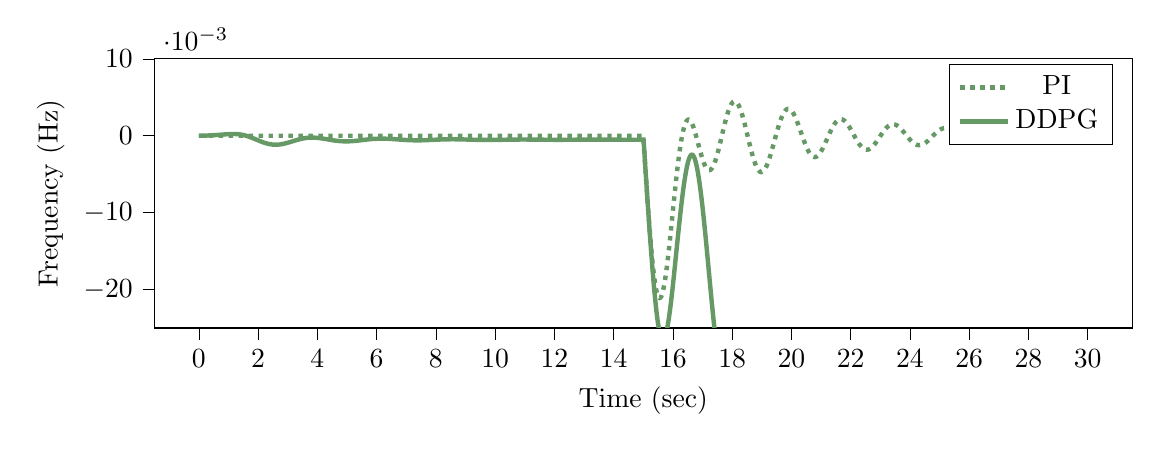
\begin{tikzpicture}

\definecolor{color0}{rgb}{0.12156862745098,0.466666666666667,0.705882352941177}
\definecolor{color1}{rgb}{1,0.498039215686275,0.0549019607843137}

\begin{axis}[
compat=newest,
tick align=outside,
tick pos=left,
x grid style={white!69.0196078431373!black},
xmin=-1.50000000000009, xmax=31.500000000002,
xtick style={color=black},
y grid style={white!69.0196078431373!black},
ymin=-0.025, ymax=0.01,
ytick style={color=black},
%yticklabel style={
%        /pgf/number format/.cd,
%        	fixed,
%        	fixed zerofill,
%         	precision=3,
%        /tikz/.cd
%},
scaled y ticks=true,
scaled y ticks=base 10:3,
width=14cm,
height=5cm,
xlabel=Time (sec),
ylabel=Frequency (Hz)
%y label style={at={(-0.2,0.5)}}
]

\addplot [ultra thick, green!20!gray, dotted]
table {%
0 0
0.01 0
0.02 0
0.03 0
0.04 0
0.05 0
0.06 0
0.07 0
0.08 0
0.09 0
0.1 0
0.11 0
0.12 0
0.13 0
0.14 0
0.15 0
0.16 0
0.17 0
0.18 0
0.19 0
0.2 0
0.21 0
0.22 0
0.23 0
0.24 0
0.25 0
0.26 0
0.27 0
0.28 0
0.29 0
0.3 0
0.31 0
0.32 0
0.33 0
0.34 0
0.35 0
0.36 0
0.37 0
0.38 0
0.39 0
0.4 0
0.41 0
0.42 0
0.43 0
0.44 0
0.45 0
0.46 0
0.47 0
0.48 0
0.49 0
0.5 0
0.51 0
0.52 0
0.53 0
0.54 0
0.55 0
0.56 0
0.57 0
0.58 0
0.59 0
0.6 0
0.61 0
0.62 0
0.63 0
0.64 0
0.65 0
0.66 0
0.67 0
0.68 0
0.69 0
0.7 0
0.71 0
0.72 0
0.73 0
0.74 0
0.75 0
0.76 0
0.77 0
0.78 0
0.79 0
0.8 0
0.81 0
0.820000000000001 0
0.830000000000001 0
0.840000000000001 0
0.850000000000001 0
0.860000000000001 0
0.870000000000001 0
0.880000000000001 0
0.890000000000001 0
0.900000000000001 0
0.910000000000001 0
0.920000000000001 0
0.930000000000001 0
0.940000000000001 0
0.950000000000001 0
0.960000000000001 0
0.970000000000001 0
0.980000000000001 0
0.990000000000001 0
1 0
1.01 0
1.02 0
1.03 0
1.04 0
1.05 0
1.06 0
1.07 0
1.08 0
1.09 0
1.1 0
1.11 0
1.12 0
1.13 0
1.14 0
1.15 0
1.16 0
1.17 0
1.18 0
1.19 0
1.2 0
1.21 0
1.22 0
1.23 0
1.24 0
1.25 0
1.26 0
1.27 0
1.28 0
1.29 0
1.3 0
1.31 0
1.32 0
1.33 0
1.34 0
1.35 0
1.36 0
1.37 0
1.38 0
1.39 0
1.4 0
1.41 0
1.42 0
1.43 0
1.44 0
1.45 0
1.46 0
1.47 0
1.48 0
1.49 0
1.5 0
1.51 0
1.52 0
1.53 0
1.54 0
1.55 0
1.56 0
1.57 0
1.58 0
1.59 0
1.6 0
1.61 0
1.62 0
1.63 0
1.64 0
1.65 0
1.66 0
1.67 0
1.68 0
1.69 0
1.7 0
1.71 0
1.72 0
1.73 0
1.74 0
1.75 0
1.76 0
1.77 0
1.78 0
1.79 0
1.8 0
1.81 0
1.82 0
1.83 0
1.84 0
1.85 0
1.86 0
1.87 0
1.88 0
1.89 0
1.9 0
1.91 0
1.92 0
1.93 0
1.94 0
1.95 0
1.96 0
1.97 0
1.98 0
1.99 0
2 0
2.01 0
2.02 0
2.03 0
2.04 0
2.05 0
2.06 0
2.07 0
2.08 0
2.09 0
2.1 0
2.11 0
2.12 0
2.13 0
2.14 0
2.15 0
2.16 0
2.17 0
2.18 0
2.19 0
2.2 0
2.21 0
2.22 0
2.23 0
2.24 0
2.25 0
2.26 0
2.27 0
2.28 0
2.29 0
2.29999999999999 0
2.30999999999999 0
2.31999999999999 0
2.32999999999999 0
2.33999999999999 0
2.34999999999999 0
2.35999999999999 0
2.36999999999999 0
2.37999999999999 0
2.38999999999999 0
2.39999999999999 0
2.40999999999999 0
2.41999999999999 0
2.42999999999999 0
2.43999999999999 0
2.44999999999999 0
2.45999999999999 0
2.46999999999999 0
2.47999999999999 0
2.48999999999999 0
2.49999999999999 0
2.50999999999999 0
2.51999999999999 0
2.52999999999999 0
2.53999999999999 0
2.54999999999999 0
2.55999999999999 0
2.56999999999999 0
2.57999999999999 0
2.58999999999999 0
2.59999999999999 0
2.60999999999999 0
2.61999999999999 0
2.62999999999999 0
2.63999999999999 0
2.64999999999999 0
2.65999999999999 0
2.66999999999999 0
2.67999999999999 0
2.68999999999999 0
2.69999999999999 0
2.70999999999999 0
2.71999999999999 0
2.72999999999999 0
2.73999999999999 0
2.74999999999999 0
2.75999999999999 0
2.76999999999998 0
2.77999999999998 0
2.78999999999998 0
2.79999999999998 0
2.80999999999998 0
2.81999999999998 0
2.82999999999998 0
2.83999999999998 0
2.84999999999998 0
2.85999999999998 0
2.86999999999998 0
2.87999999999998 0
2.88999999999998 0
2.89999999999998 0
2.90999999999998 0
2.91999999999998 0
2.92999999999998 0
2.93999999999998 0
2.94999999999998 0
2.95999999999998 0
2.96999999999998 0
2.97999999999998 0
2.98999999999998 0
2.99999999999998 0
3.00999999999998 0
3.01999999999998 0
3.02999999999998 0
3.03999999999998 0
3.04999999999998 0
3.05999999999998 0
3.06999999999998 0
3.07999999999998 0
3.08999999999998 0
3.09999999999998 0
3.10999999999998 0
3.11999999999998 0
3.12999999999998 0
3.13999999999998 0
3.14999999999998 0
3.15999999999998 0
3.16999999999998 0
3.17999999999998 0
3.18999999999998 0
3.19999999999998 0
3.20999999999998 0
3.21999999999998 0
3.22999999999998 0
3.23999999999997 0
3.24999999999997 0
3.25999999999997 0
3.26999999999997 0
3.27999999999997 0
3.28999999999997 0
3.29999999999997 0
3.30999999999997 0
3.31999999999997 0
3.32999999999997 0
3.33999999999997 0
3.34999999999997 0
3.35999999999997 0
3.36999999999997 0
3.37999999999997 0
3.38999999999997 0
3.39999999999997 0
3.40999999999997 0
3.41999999999997 0
3.42999999999997 0
3.43999999999997 0
3.44999999999997 0
3.45999999999997 0
3.46999999999997 0
3.47999999999997 0
3.48999999999997 0
3.49999999999997 0
3.50999999999997 0
3.51999999999997 0
3.52999999999997 0
3.53999999999997 0
3.54999999999997 0
3.55999999999997 0
3.56999999999997 0
3.57999999999997 0
3.58999999999997 0
3.59999999999997 0
3.60999999999997 0
3.61999999999997 0
3.62999999999997 0
3.63999999999997 0
3.64999999999997 0
3.65999999999997 0
3.66999999999997 0
3.67999999999997 0
3.68999999999997 0
3.69999999999997 0
3.70999999999996 0
3.71999999999996 0
3.72999999999996 0
3.73999999999996 0
3.74999999999996 0
3.75999999999996 0
3.76999999999996 0
3.77999999999996 0
3.78999999999996 0
3.79999999999996 0
3.80999999999996 0
3.81999999999996 0
3.82999999999996 0
3.83999999999996 0
3.84999999999996 0
3.85999999999996 0
3.86999999999996 0
3.87999999999996 0
3.88999999999996 0
3.89999999999996 0
3.90999999999996 0
3.91999999999996 0
3.92999999999996 0
3.93999999999996 0
3.94999999999996 0
3.95999999999996 0
3.96999999999996 0
3.97999999999996 0
3.98999999999996 0
3.99999999999996 0
4.00999999999996 0
4.01999999999996 0
4.02999999999996 0
4.03999999999996 0
4.04999999999996 0
4.05999999999996 0
4.06999999999996 0
4.07999999999996 0
4.08999999999996 0
4.09999999999996 0
4.10999999999996 0
4.11999999999996 0
4.12999999999996 0
4.13999999999996 0
4.14999999999996 0
4.15999999999996 0
4.16999999999996 0
4.17999999999996 0
4.18999999999996 0
4.19999999999995 0
4.20999999999995 0
4.21999999999995 0
4.22999999999995 0
4.23999999999995 0
4.24999999999995 0
4.25999999999995 0
4.26999999999995 0
4.27999999999995 0
4.28999999999995 0
4.29999999999995 0
4.30999999999995 0
4.31999999999995 0
4.32999999999995 0
4.33999999999995 0
4.34999999999995 0
4.35999999999995 0
4.36999999999995 0
4.37999999999995 0
4.38999999999995 0
4.39999999999995 0
4.40999999999995 0
4.41999999999995 0
4.42999999999995 0
4.43999999999995 0
4.44999999999995 0
4.45999999999995 0
4.46999999999995 0
4.47999999999995 0
4.48999999999995 0
4.49999999999995 0
4.50999999999995 0
4.51999999999995 0
4.52999999999995 0
4.53999999999995 0
4.54999999999995 0
4.55999999999995 0
4.56999999999995 0
4.57999999999995 0
4.58999999999995 0
4.59999999999995 0
4.60999999999995 0
4.61999999999995 0
4.62999999999995 0
4.63999999999995 0
4.64999999999995 0
4.65999999999995 0
4.66999999999994 0
4.67999999999994 0
4.68999999999994 0
4.69999999999994 0
4.70999999999994 0
4.71999999999994 0
4.72999999999994 0
4.73999999999994 0
4.74999999999994 0
4.75999999999994 0
4.76999999999994 0
4.77999999999994 0
4.78999999999994 0
4.79999999999994 0
4.80999999999994 0
4.81999999999994 0
4.82999999999994 0
4.83999999999994 0
4.84999999999994 0
4.85999999999994 0
4.86999999999994 0
4.87999999999994 0
4.88999999999994 0
4.89999999999994 0
4.90999999999994 0
4.91999999999994 0
4.92999999999994 0
4.93999999999994 0
4.94999999999994 0
4.95999999999994 0
4.96999999999994 0
4.97999999999994 0
4.98999999999994 0
4.99999999999994 0
5.00999999999994 0
5.01999999999994 0
5.02999999999994 0
5.03999999999994 0
5.04999999999994 0
5.05999999999994 0
5.06999999999994 0
5.07999999999994 0
5.08999999999994 0
5.09999999999994 0
5.10999999999994 0
5.11999999999994 0
5.12999999999994 0
5.13999999999993 0
5.14999999999993 0
5.15999999999993 0
5.16999999999993 0
5.17999999999993 0
5.18999999999993 0
5.19999999999993 0
5.20999999999993 0
5.21999999999993 0
5.22999999999993 0
5.23999999999993 0
5.24999999999993 0
5.25999999999993 0
5.26999999999993 0
5.27999999999993 0
5.28999999999993 0
5.29999999999993 0
5.30999999999993 0
5.31999999999993 0
5.32999999999993 0
5.33999999999993 0
5.34999999999993 0
5.35999999999993 0
5.36999999999993 0
5.37999999999993 0
5.38999999999993 0
5.39999999999993 0
5.40999999999993 0
5.41999999999993 0
5.42999999999993 0
5.43999999999993 0
5.44999999999993 0
5.45999999999993 0
5.46999999999993 0
5.47999999999993 0
5.48999999999993 0
5.49999999999993 0
5.50999999999993 0
5.51999999999993 0
5.52999999999993 0
5.53999999999993 0
5.54999999999993 0
5.55999999999993 0
5.56999999999993 0
5.57999999999993 0
5.58999999999993 0
5.59999999999993 0
5.60999999999992 0
5.61999999999992 0
5.62999999999992 0
5.63999999999992 0
5.64999999999992 0
5.65999999999992 0
5.66999999999992 0
5.67999999999992 0
5.68999999999992 0
5.69999999999992 0
5.70999999999992 0
5.71999999999992 0
5.72999999999992 0
5.73999999999992 0
5.74999999999992 0
5.75999999999992 0
5.76999999999992 0
5.77999999999992 0
5.78999999999992 0
5.79999999999992 0
5.80999999999992 0
5.81999999999992 0
5.82999999999992 0
5.83999999999992 0
5.84999999999992 0
5.85999999999992 0
5.86999999999992 0
5.87999999999992 0
5.88999999999992 0
5.89999999999992 0
5.90999999999992 0
5.91999999999992 0
5.92999999999992 0
5.93999999999992 0
5.94999999999992 0
5.95999999999992 0
5.96999999999992 0
5.97999999999992 0
5.98999999999992 0
5.99999999999992 0
6.00999999999992 0
6.01999999999992 0
6.02999999999992 0
6.03999999999992 0
6.04999999999992 0
6.05999999999992 0
6.06999999999992 0
6.07999999999991 0
6.08999999999991 0
6.09999999999991 0
6.10999999999991 0
6.11999999999991 0
6.12999999999991 0
6.13999999999991 0
6.14999999999991 0
6.15999999999991 0
6.16999999999991 0
6.17999999999991 0
6.18999999999991 0
6.19999999999991 0
6.20999999999991 0
6.21999999999991 0
6.22999999999991 0
6.23999999999991 0
6.24999999999991 0
6.25999999999991 0
6.26999999999991 0
6.27999999999991 0
6.28999999999991 0
6.29999999999991 0
6.30999999999991 0
6.31999999999991 0
6.32999999999991 0
6.33999999999991 0
6.34999999999991 0
6.35999999999991 0
6.36999999999991 0
6.37999999999991 0
6.38999999999991 0
6.39999999999991 0
6.40999999999991 0
6.41999999999991 0
6.42999999999991 0
6.43999999999991 0
6.44999999999991 0
6.45999999999991 0
6.46999999999991 0
6.47999999999991 0
6.48999999999991 0
6.49999999999991 0
6.50999999999991 0
6.51999999999991 0
6.52999999999991 0
6.53999999999991 0
6.5499999999999 0
6.5599999999999 0
6.5699999999999 0
6.5799999999999 0
6.5899999999999 0
6.5999999999999 0
6.6099999999999 0
6.6199999999999 0
6.6299999999999 0
6.6399999999999 0
6.6499999999999 0
6.6599999999999 0
6.6699999999999 0
6.6799999999999 0
6.6899999999999 0
6.6999999999999 0
6.7099999999999 0
6.7199999999999 0
6.7299999999999 0
6.7399999999999 0
6.7499999999999 0
6.7599999999999 0
6.7699999999999 0
6.7799999999999 0
6.7899999999999 0
6.7999999999999 0
6.8099999999999 0
6.8199999999999 0
6.8299999999999 0
6.8399999999999 0
6.8499999999999 0
6.8599999999999 0
6.8699999999999 0
6.8799999999999 0
6.8899999999999 0
6.8999999999999 0
6.9099999999999 0
6.9199999999999 0
6.9299999999999 0
6.9399999999999 0
6.9499999999999 0
6.9599999999999 0
6.9699999999999 0
6.9799999999999 0
6.9899999999999 0
6.9999999999999 0
7.00999999999989 0
7.01999999999989 0
7.02999999999989 0
7.03999999999989 0
7.04999999999989 0
7.05999999999989 0
7.06999999999989 0
7.07999999999989 0
7.08999999999989 0
7.09999999999989 0
7.10999999999989 0
7.11999999999989 0
7.12999999999989 0
7.13999999999989 0
7.14999999999989 0
7.15999999999989 0
7.16999999999989 0
7.17999999999989 0
7.18999999999989 0
7.19999999999989 0
7.20999999999989 0
7.21999999999989 0
7.22999999999989 0
7.23999999999989 0
7.24999999999989 0
7.25999999999989 0
7.26999999999989 0
7.27999999999989 0
7.28999999999989 0
7.29999999999989 0
7.30999999999989 0
7.31999999999989 0
7.32999999999989 0
7.33999999999989 0
7.34999999999989 0
7.35999999999989 0
7.36999999999989 0
7.37999999999989 0
7.38999999999989 0
7.39999999999989 0
7.40999999999989 0
7.41999999999989 0
7.42999999999989 0
7.43999999999989 0
7.44999999999989 0
7.45999999999989 0
7.46999999999989 0
7.47999999999988 0
7.48999999999988 0
7.49999999999988 0
7.50999999999988 0
7.51999999999988 0
7.52999999999988 0
7.53999999999988 0
7.54999999999988 0
7.55999999999988 0
7.56999999999988 0
7.57999999999988 0
7.58999999999988 0
7.59999999999988 0
7.60999999999988 0
7.61999999999988 0
7.62999999999988 0
7.63999999999988 0
7.64999999999988 0
7.65999999999988 0
7.66999999999988 0
7.67999999999988 0
7.68999999999988 0
7.69999999999988 0
7.70999999999988 0
7.71999999999988 0
7.72999999999988 0
7.73999999999988 0
7.74999999999988 0
7.75999999999988 0
7.76999999999988 0
7.77999999999988 0
7.78999999999988 0
7.79999999999988 0
7.80999999999988 0
7.81999999999988 0
7.82999999999988 0
7.83999999999988 0
7.84999999999988 0
7.85999999999988 0
7.86999999999988 0
7.87999999999988 0
7.88999999999988 0
7.89999999999988 0
7.90999999999988 0
7.91999999999988 0
7.92999999999988 0
7.93999999999988 0
7.94999999999987 0
7.95999999999987 0
7.96999999999987 0
7.97999999999987 0
7.98999999999987 0
7.99999999999987 0
8.00999999999987 0
8.01999999999987 0
8.02999999999987 0
8.03999999999987 0
8.04999999999987 0
8.05999999999987 0
8.06999999999987 0
8.07999999999987 0
8.08999999999987 0
8.09999999999987 0
8.10999999999987 0
8.11999999999987 0
8.12999999999987 0
8.13999999999987 0
8.14999999999987 0
8.15999999999987 0
8.16999999999987 0
8.17999999999987 0
8.18999999999987 0
8.19999999999987 0
8.20999999999987 0
8.21999999999987 0
8.22999999999987 0
8.23999999999987 0
8.24999999999987 0
8.25999999999987 0
8.26999999999987 0
8.27999999999987 0
8.28999999999987 0
8.29999999999987 0
8.30999999999987 0
8.31999999999987 0
8.32999999999987 0
8.33999999999987 0
8.34999999999987 0
8.35999999999987 0
8.36999999999987 0
8.37999999999987 0
8.38999999999987 0
8.39999999999987 0
8.40999999999987 0
8.41999999999986 0
8.42999999999986 0
8.43999999999986 0
8.44999999999986 0
8.45999999999986 0
8.46999999999986 0
8.47999999999986 0
8.48999999999986 0
8.49999999999986 0
8.50999999999986 0
8.51999999999986 0
8.52999999999986 0
8.53999999999986 0
8.54999999999986 0
8.55999999999986 0
8.56999999999986 0
8.57999999999986 0
8.58999999999986 0
8.59999999999986 0
8.60999999999986 0
8.61999999999986 0
8.62999999999986 0
8.63999999999986 0
8.64999999999986 0
8.65999999999986 0
8.66999999999986 0
8.67999999999986 0
8.68999999999986 0
8.69999999999986 0
8.70999999999986 0
8.71999999999986 0
8.72999999999986 0
8.73999999999986 0
8.74999999999986 0
8.75999999999986 0
8.76999999999986 0
8.77999999999986 0
8.78999999999986 0
8.79999999999986 0
8.80999999999986 0
8.81999999999986 0
8.82999999999986 0
8.83999999999986 0
8.84999999999986 0
8.85999999999986 0
8.86999999999986 0
8.87999999999986 0
8.88999999999985 0
8.89999999999985 0
8.90999999999985 0
8.91999999999985 0
8.92999999999985 0
8.93999999999985 0
8.94999999999985 0
8.95999999999985 0
8.96999999999985 0
8.97999999999985 0
8.98999999999985 0
8.99999999999985 0
9.00999999999985 0
9.01999999999985 0
9.02999999999985 0
9.03999999999985 0
9.04999999999985 0
9.05999999999985 0
9.06999999999985 0
9.07999999999985 0
9.08999999999985 0
9.09999999999985 0
9.10999999999985 0
9.11999999999985 0
9.12999999999985 0
9.13999999999985 0
9.14999999999985 0
9.15999999999985 0
9.16999999999985 0
9.17999999999985 0
9.18999999999985 0
9.19999999999985 0
9.20999999999985 0
9.21999999999985 0
9.22999999999985 0
9.23999999999985 0
9.24999999999985 0
9.25999999999985 0
9.26999999999985 0
9.27999999999985 0
9.28999999999985 0
9.29999999999985 0
9.30999999999985 0
9.31999999999985 0
9.32999999999985 0
9.33999999999985 0
9.34999999999985 0
9.35999999999984 0
9.36999999999984 0
9.37999999999984 0
9.38999999999984 0
9.39999999999984 0
9.40999999999984 0
9.41999999999984 0
9.42999999999984 0
9.43999999999984 0
9.44999999999984 0
9.45999999999984 0
9.46999999999984 0
9.47999999999984 0
9.48999999999984 0
9.49999999999984 0
9.50999999999984 0
9.51999999999984 0
9.52999999999984 0
9.53999999999984 0
9.54999999999984 0
9.55999999999984 0
9.56999999999984 0
9.57999999999984 0
9.58999999999984 0
9.59999999999984 0
9.60999999999984 0
9.61999999999984 0
9.62999999999984 0
9.63999999999984 0
9.64999999999984 0
9.65999999999984 0
9.66999999999984 0
9.67999999999984 0
9.68999999999984 0
9.69999999999984 0
9.70999999999984 0
9.71999999999984 0
9.72999999999984 0
9.73999999999984 0
9.74999999999984 0
9.75999999999984 0
9.76999999999984 0
9.77999999999984 0
9.78999999999984 0
9.79999999999984 0
9.80999999999984 0
9.81999999999984 0
9.82999999999983 0
9.83999999999983 0
9.84999999999983 0
9.85999999999983 0
9.86999999999983 0
9.87999999999983 0
9.88999999999983 0
9.89999999999983 0
9.90999999999983 0
9.91999999999983 0
9.92999999999983 0
9.93999999999983 0
9.94999999999983 0
9.95999999999983 0
9.96999999999983 0
9.97999999999983 0
9.98999999999983 0
9.99999999999983 0
10.0099999999998 0
10.0199999999998 0
10.0299999999998 0
10.0399999999998 0
10.0499999999998 0
10.0599999999998 0
10.0699999999998 0
10.0799999999998 0
10.0899999999998 0
10.0999999999998 0
10.1099999999998 0
10.1199999999998 0
10.1299999999998 0
10.1399999999998 0
10.1499999999998 0
10.1599999999998 0
10.1699999999998 0
10.1799999999998 0
10.1899999999998 0
10.1999999999998 0
10.2099999999998 0
10.2199999999998 0
10.2299999999998 0
10.2399999999998 0
10.2499999999998 0
10.2599999999998 0
10.2699999999998 0
10.2799999999998 0
10.2899999999998 0
10.2999999999998 0
10.3099999999998 0
10.3199999999998 0
10.3299999999998 0
10.3399999999998 0
10.3499999999998 0
10.3599999999998 0
10.3699999999998 0
10.3799999999998 0
10.3899999999998 0
10.3999999999998 0
10.4099999999998 0
10.4199999999998 0
10.4299999999998 0
10.4399999999998 0
10.4499999999998 0
10.4599999999998 0
10.4699999999998 0
10.4799999999998 0
10.4899999999998 0
10.4999999999998 0
10.5099999999998 0
10.5199999999998 0
10.5299999999998 0
10.5399999999998 0
10.5499999999998 0
10.5599999999998 0
10.5699999999998 0
10.5799999999998 0
10.5899999999998 0
10.5999999999998 0
10.6099999999998 0
10.6199999999998 0
10.6299999999998 0
10.6399999999998 0
10.6499999999998 0
10.6599999999998 0
10.6699999999998 0
10.6799999999998 0
10.6899999999998 0
10.6999999999998 0
10.7099999999998 0
10.7199999999998 0
10.7299999999998 0
10.7399999999998 0
10.7499999999998 0
10.7599999999998 0
10.7699999999998 0
10.7799999999998 0
10.7899999999998 0
10.7999999999998 0
10.8099999999998 0
10.8199999999998 0
10.8299999999998 0
10.8399999999998 0
10.8499999999998 0
10.8599999999998 0
10.8699999999998 0
10.8799999999998 0
10.8899999999998 0
10.8999999999998 0
10.9099999999998 0
10.9199999999998 0
10.9299999999998 0
10.9399999999998 0
10.9499999999998 0
10.9599999999998 0
10.9699999999998 0
10.9799999999998 0
10.9899999999998 0
10.9999999999998 0
11.0099999999998 0
11.0199999999998 0
11.0299999999998 0
11.0399999999998 0
11.0499999999998 0
11.0599999999998 0
11.0699999999998 0
11.0799999999998 0
11.0899999999998 0
11.0999999999998 0
11.1099999999998 0
11.1199999999998 0
11.1299999999998 0
11.1399999999998 0
11.1499999999998 0
11.1599999999998 0
11.1699999999998 0
11.1799999999998 0
11.1899999999998 0
11.1999999999998 0
11.2099999999998 0
11.2199999999998 0
11.2299999999998 0
11.2399999999998 0
11.2499999999998 0
11.2599999999998 0
11.2699999999998 0
11.2799999999998 0
11.2899999999998 0
11.2999999999998 0
11.3099999999998 0
11.3199999999998 0
11.3299999999998 0
11.3399999999998 0
11.3499999999998 0
11.3599999999998 0
11.3699999999998 0
11.3799999999998 0
11.3899999999998 0
11.3999999999998 0
11.4099999999998 0
11.4199999999998 0
11.4299999999998 0
11.4399999999998 0
11.4499999999998 0
11.4599999999998 0
11.4699999999998 0
11.4799999999998 0
11.4899999999998 0
11.4999999999998 0
11.5099999999998 0
11.5199999999998 0
11.5299999999998 0
11.5399999999998 0
11.5499999999998 0
11.5599999999998 0
11.5699999999998 0
11.5799999999998 0
11.5899999999998 0
11.5999999999998 0
11.6099999999998 0
11.6199999999998 0
11.6299999999998 0
11.6399999999998 0
11.6499999999998 0
11.6599999999998 0
11.6699999999998 0
11.6799999999998 0
11.6899999999998 0
11.6999999999998 0
11.7099999999998 0
11.7199999999998 0
11.7299999999998 0
11.7399999999998 0
11.7499999999998 0
11.7599999999998 0
11.7699999999998 0
11.7799999999998 0
11.7899999999998 0
11.7999999999998 0
11.8099999999998 0
11.8199999999998 0
11.8299999999998 0
11.8399999999998 0
11.8499999999998 0
11.8599999999998 0
11.8699999999998 0
11.8799999999998 0
11.8899999999998 0
11.8999999999998 0
11.9099999999998 0
11.9199999999998 0
11.9299999999998 0
11.9399999999998 0
11.9499999999998 0
11.9599999999998 0
11.9699999999998 0
11.9799999999998 0
11.9899999999998 0
11.9999999999998 0
12.0099999999998 0
12.0199999999998 0
12.0299999999998 0
12.0399999999998 0
12.0499999999998 0
12.0599999999998 0
12.0699999999998 0
12.0799999999998 0
12.0899999999998 0
12.0999999999998 0
12.1099999999998 0
12.1199999999998 0
12.1299999999998 0
12.1399999999998 0
12.1499999999998 0
12.1599999999998 0
12.1699999999998 0
12.1799999999998 0
12.1899999999998 0
12.1999999999998 0
12.2099999999998 0
12.2199999999998 0
12.2299999999998 0
12.2399999999998 0
12.2499999999998 0
12.2599999999998 0
12.2699999999998 0
12.2799999999998 0
12.2899999999998 0
12.2999999999998 0
12.3099999999998 0
12.3199999999998 0
12.3299999999998 0
12.3399999999998 0
12.3499999999998 0
12.3599999999998 0
12.3699999999998 0
12.3799999999998 0
12.3899999999998 0
12.3999999999998 0
12.4099999999998 0
12.4199999999998 0
12.4299999999998 0
12.4399999999998 0
12.4499999999998 0
12.4599999999998 0
12.4699999999998 0
12.4799999999998 0
12.4899999999998 0
12.4999999999998 0
12.5099999999998 0
12.5199999999998 0
12.5299999999998 0
12.5399999999998 0
12.5499999999998 0
12.5599999999998 0
12.5699999999998 0
12.5799999999998 0
12.5899999999998 0
12.5999999999998 0
12.6099999999998 0
12.6199999999998 0
12.6299999999998 0
12.6399999999998 0
12.6499999999998 0
12.6599999999998 0
12.6699999999998 0
12.6799999999998 0
12.6899999999998 0
12.6999999999998 0
12.7099999999998 0
12.7199999999998 0
12.7299999999998 0
12.7399999999998 0
12.7499999999998 0
12.7599999999998 0
12.7699999999998 0
12.7799999999998 0
12.7899999999998 0
12.7999999999998 0
12.8099999999998 0
12.8199999999998 0
12.8299999999998 0
12.8399999999998 0
12.8499999999998 0
12.8599999999998 0
12.8699999999998 0
12.8799999999998 0
12.8899999999998 0
12.8999999999998 0
12.9099999999998 0
12.9199999999998 0
12.9299999999998 0
12.9399999999998 0
12.9499999999998 0
12.9599999999998 0
12.9699999999998 0
12.9799999999998 0
12.9899999999998 0
12.9999999999998 0
13.0099999999998 0
13.0199999999998 0
13.0299999999998 0
13.0399999999998 0
13.0499999999998 0
13.0599999999998 0
13.0699999999998 0
13.0799999999998 0
13.0899999999998 0
13.0999999999998 0
13.1099999999998 0
13.1199999999998 0
13.1299999999998 0
13.1399999999998 0
13.1499999999998 0
13.1599999999998 0
13.1699999999998 0
13.1799999999998 0
13.1899999999998 0
13.1999999999998 0
13.2099999999998 0
13.2199999999998 0
13.2299999999998 0
13.2399999999998 0
13.2499999999998 0
13.2599999999998 0
13.2699999999998 0
13.2799999999998 0
13.2899999999998 0
13.2999999999998 0
13.3099999999998 0
13.3199999999998 0
13.3299999999998 0
13.3399999999998 0
13.3499999999998 0
13.3599999999998 0
13.3699999999998 0
13.3799999999998 0
13.3899999999998 0
13.3999999999998 0
13.4099999999998 0
13.4199999999998 0
13.4299999999998 0
13.4399999999998 0
13.4499999999998 0
13.4599999999998 0
13.4699999999998 0
13.4799999999998 0
13.4899999999998 0
13.4999999999998 0
13.5099999999998 0
13.5199999999998 0
13.5299999999998 0
13.5399999999998 0
13.5499999999998 0
13.5599999999998 0
13.5699999999998 0
13.5799999999998 0
13.5899999999998 0
13.5999999999998 0
13.6099999999998 0
13.6199999999998 0
13.6299999999998 0
13.6399999999998 0
13.6499999999998 0
13.6599999999998 0
13.6699999999998 0
13.6799999999998 0
13.6899999999998 0
13.6999999999998 0
13.7099999999998 0
13.7199999999998 0
13.7299999999998 0
13.7399999999998 0
13.7499999999998 0
13.7599999999998 0
13.7699999999998 0
13.7799999999998 0
13.7899999999998 0
13.7999999999998 0
13.8099999999998 0
13.8199999999997 0
13.8299999999997 0
13.8399999999997 0
13.8499999999997 0
13.8599999999997 0
13.8699999999997 0
13.8799999999997 0
13.8899999999997 0
13.8999999999997 0
13.9099999999997 0
13.9199999999997 0
13.9299999999997 0
13.9399999999997 0
13.9499999999997 0
13.9599999999997 0
13.9699999999997 0
13.9799999999997 0
13.9899999999997 0
13.9999999999997 0
14.0099999999997 0
14.0199999999997 0
14.0299999999997 0
14.0399999999997 0
14.0499999999997 0
14.0599999999997 0
14.0699999999997 0
14.0799999999997 0
14.0899999999997 0
14.0999999999997 0
14.1099999999997 0
14.1199999999997 0
14.1299999999997 0
14.1399999999997 0
14.1499999999997 0
14.1599999999997 0
14.1699999999997 0
14.1799999999997 0
14.1899999999997 0
14.1999999999997 0
14.2099999999997 0
14.2199999999997 0
14.2299999999997 0
14.2399999999997 0
14.2499999999997 0
14.2599999999997 0
14.2699999999997 0
14.2799999999997 0
14.2899999999997 0
14.2999999999997 0
14.3099999999997 0
14.3199999999997 0
14.3299999999997 0
14.3399999999997 0
14.3499999999997 0
14.3599999999997 0
14.3699999999997 0
14.3799999999997 0
14.3899999999997 0
14.3999999999997 0
14.4099999999997 0
14.4199999999997 0
14.4299999999997 0
14.4399999999997 0
14.4499999999997 0
14.4599999999997 0
14.4699999999997 0
14.4799999999997 0
14.4899999999997 0
14.4999999999997 0
14.5099999999997 0
14.5199999999997 0
14.5299999999997 0
14.5399999999997 0
14.5499999999997 0
14.5599999999997 0
14.5699999999997 0
14.5799999999997 0
14.5899999999997 0
14.5999999999997 0
14.6099999999997 0
14.6199999999997 0
14.6299999999997 0
14.6399999999997 0
14.6499999999997 0
14.6599999999997 0
14.6699999999997 0
14.6799999999997 0
14.6899999999997 0
14.6999999999997 0
14.7099999999997 0
14.7199999999997 0
14.7299999999997 0
14.7399999999997 0
14.7499999999997 0
14.7599999999997 0
14.7699999999997 0
14.7799999999997 0
14.7899999999997 0
14.7999999999997 0
14.8099999999997 0
14.8199999999997 0
14.8299999999997 0
14.8399999999997 0
14.8499999999997 0
14.8599999999997 0
14.8699999999997 0
14.8799999999997 0
14.8899999999997 0
14.8999999999997 0
14.9099999999997 0
14.9199999999997 0
14.9299999999997 0
14.9399999999997 0
14.9499999999997 0
14.9599999999997 0
14.9699999999997 0
14.9799999999997 0
14.9899999999997 0
14.9999999999997 -3.93651211614443e-09
15.0099999999997 -0.000599816270682417
15.0199999999997 -0.00119908880084479
15.0299999999997 -0.00179754253372852
15.0399999999997 -0.0023948446344429
15.0499999999997 -0.00299062124939138
15.0599999999997 -0.00358446368618463
15.0699999999997 -0.00417593452179766
15.0799999999997 -0.00476457277282835
15.0899999999997 -0.00534989852308608
15.0999999999997 -0.00593141709971282
15.1099999999997 -0.00650862278845816
15.1199999999997 -0.00708100214101138
15.1299999999997 -0.00764803692388741
15.1399999999997 -0.00820920675160281
15.1499999999997 -0.00876399144127596
15.1599999999997 -0.00931187312100392
15.1699999999997 -0.00985233812025386
15.1799999999997 -0.0103848786669187
15.1899999999997 -0.0109089944125681
15.1999999999997 -0.0114241938047095
15.2099999999997 -0.0119299953224874
15.2199999999997 -0.0124259285901838
15.2299999999997 -0.0129115353810624
15.2399999999997 -0.0133863705225182
15.2499999999997 -0.0138500027121151
15.2599999999997 -0.0143020152528775
15.2699999999997 -0.0147420067151584
15.2799999999997 -0.0151695915314819
15.2899999999997 -0.0155844005299559
15.2999999999997 -0.0159860814111557
15.3099999999997 -0.0163742991727683
15.3199999999997 -0.0167487364857575
15.3299999999997 -0.0171090940253509
15.3399999999997 -0.0174550907597512
15.3499999999997 -0.0177864641991206
15.3599999999997 -0.0181029706070963
15.3699999999997 -0.0184043851768254
15.3799999999997 -0.0186905021732893
15.3899999999997 -0.0189611350434885
15.3999999999997 -0.0192161164958972
15.4099999999997 -0.0194552985504484
15.4199999999997 -0.0196785525601916
15.4299999999997 -0.0198857692056582
15.4399999999997 -0.0200768584641575
15.4499999999997 -0.0202517495499544
15.4599999999997 -0.0204103908330175
15.4699999999997 -0.0205527497331997
15.4799999999997 -0.0206788125911258
15.4899999999997 -0.020788584517633
15.4999999999997 -0.0208820892175594
15.5099999999997 -0.0209593687961681
15.5199999999997 -0.0210204835436248
15.5299999999997 -0.0210655116994115
15.5399999999997 -0.0210945491972521
15.5499999999997 -0.0211077093911169
15.5599999999997 -0.0211051227628629
15.5699999999997 -0.0210869366120657
15.5799999999997 -0.0210533147283251
15.5899999999997 -0.0210044370457204
15.5999999999997 -0.020940499661103
15.6099999999997 -0.02086171413124
15.6199999999997 -0.0207683066693864
15.6299999999997 -0.020660518109462
15.6399999999997 -0.0205386034887037
15.6499999999997 -0.0204028316172527
15.6599999999997 -0.0202534846352881
15.6699999999997 -0.0200908575583267
15.6799999999997 -0.0199152578113132
15.6899999999997 -0.0197270047521316
15.6999999999997 -0.0195264291881473
15.7099999999997 -0.0193138729363691
15.7199999999997 -0.0190896890340603
15.7299999999997 -0.0188542395663603
15.7399999999997 -0.0186078960302049
15.7499999999997 -0.0183510388078863
15.7599999999997 -0.0180840566345368
15.7699999999997 -0.0178073460601992
15.7799999999997 -0.0175213109087395
15.7899999999997 -0.0172263617280233
15.7999999999997 -0.016922915240841
15.8099999999997 -0.01661139379293
15.8199999999997 -0.0162922247980807
15.8299999999997 -0.0159658401796997
15.8399999999997 -0.0156326758149685
15.8499999999997 -0.0152931709775959
15.8599999999997 -0.0149477677811284
15.8699999999997 -0.0145969106234627
15.8799999999997 -0.0142410456332094
15.8899999999997 -0.0138806201185429
15.8999999999997 -0.0135160820191715
15.9099999999997 -0.0131478793620514
15.9199999999997 -0.0127764597214612
15.9299999999997 -0.0124022696846984
15.9399999999997 -0.0120257543239688
15.9499999999997 -0.0116473566690436
15.9599999999997 -0.0112675171929203
15.9699999999997 -0.0108866733026251
15.9799999999997 -0.010505258837876
15.9899999999997 -0.0101237035781487
15.9999999999997 -0.00974243275867871
16.0099999999997 -0.00936186659591788
16.0199999999997 -0.00898241982295028
16.0299999999997 -0.00860450123535923
16.0399999999997 -0.00822851324802252
16.0499999999997 -0.00785485146330229
16.0599999999997 -0.00748390425088176
16.0699999999997 -0.00711605208197563
16.0799999999997 -0.00675166756085005
16.0899999999997 -0.00639111487612701
16.0999999999997 -0.00603474943086742
16.1099999999997 -0.00568291748648845
16.1199999999997 -0.00533595582082919
16.1299999999997 -0.00499419140065999
16.1399999999997 -0.00465794106892187
16.1499999999997 -0.00432751124696018
16.1599999999997 -0.00400319765199849
16.1699999999997 -0.00368528503008679
16.1799999999997 -0.0033740469047313
16.1899999999997 -0.00306974534139794
16.1999999999997 -0.00277263072806533
16.2099999999997 -0.00248294157197574
16.2199999999997 -0.00220090431271978
16.2299999999997 -0.00192673315176691
16.2399999999997 -0.0016606298985342
16.2499999999997 -0.00140278383306765
16.2599999999997 -0.00115337158538734
16.2699999999997 -0.000912557031531131
16.2799999999997 -0.000680491206307545
16.2899999999997 -0.000457312232753518
16.2999999999997 -0.000243145268269894
16.3099999999998 -3.81024673904882e-05
16.3199999999998 0.00015771713102514
16.3299999999998 0.000344227673721556
16.3399999999998 0.000521356105297853
16.3499999999998 0.000689042358774393
16.3599999999998 0.000847239440588993
16.3699999999998 0.00099591332670907
16.3799999999998 0.00113504259012152
16.3899999999998 0.00126461852068281
16.3999999999998 0.00138464501860784
16.4099999999998 0.00149513847296923
16.4199999999998 0.0015961276241521
16.4299999999998 0.00168765341074405
16.4399999999998 0.0017697688146495
16.4499999999998 0.00184253867514877
16.4599999999998 0.0019060394962789
16.4699999999998 0.00196035924092799
16.4799999999998 0.00200559710878891
16.4899999999998 0.00204186330986465
16.4999999999998 0.002069278825239
16.5099999999998 0.00208797514479422
16.5199999999998 0.00209809400051514
16.5299999999998 0.00209978802941269
16.5399999999998 0.00209321888857385
16.5499999999998 0.00207855719233783
16.5599999999998 0.00205598263621555
16.5699999999998 0.00202568367722203
16.5799999999998 0.00198785720589268
16.5899999999998 0.00194270821034066
16.5999999999998 0.00189044943275088
16.6099999999998 0.0018313010187348
16.6199999999998 0.00176549015999127
16.6299999999998 0.00169325073073661
16.6399999999998 0.00161482291837872
16.6499999999998 0.00153045285311375
16.6599999999998 0.00144039222069301
16.6699999999998 0.00134489788207572
16.6799999999998 0.00124423148626304
16.6899999999998 0.00113865907963004
16.6999999999998 0.00102845071250492
16.7099999999998 0.000913880043508624
16.7199999999998 0.00079522394216759
16.7299999999998 0.000672762090313417
16.7399999999998 0.000546776582781965
16.7499999999998 0.000417551527921705
16.7599999999998 0.000285372648420103
16.7699999999998 0.000150526882953243
16.7799999999998 1.33019891587028e-05
16.7899999999998 -0.000126013851577711
16.7999999999998 -0.00026713242708048
16.8099999999998 -0.000409765884387918
16.8199999999998 -0.000553627116548537
16.8299999999998 -0.000698430145693409
16.8399999999998 -0.000843890501892508
16.8499999999998 -0.00098972559733667
16.8599999999998 -0.00113565509539701
16.8699999999998 -0.0012814012741216
16.8799999999998 -0.00142668938373918
16.8899999999998 -0.00157124799775024
16.8999999999998 -0.00171480935719467
16.9099999999998 -0.00185710970769842
16.9199999999998 -0.00199788962890912
16.9299999999998 -0.00213689435595583
16.9399999999998 -0.00227387409255594
16.9499999999999 -0.0024085843154265
16.9599999999999 -0.00254078606962648
16.9699999999999 -0.0026702462544885
16.9799999999999 -0.00279673790004541
16.9899999999999 -0.00292004043342057
16.9999999999999 -0.00303993993496566
17.0099999999999 -0.00315622938388522
17.0199999999999 -0.00326870889309577
17.0299999999999 -0.0033771859330818
17.0399999999999 -0.00348147554452623
17.0499999999999 -0.00358140053950961
17.0599999999999 -0.00367679169108623
17.0699999999999 -0.00376748791106192
17.0799999999999 -0.00385333641581433
17.0899999999999 -0.003934192880012
17.0999999999999 -0.00400992157749018
17.1099999999999 -0.00408039550496184
17.1199999999999 -0.00414549651157067
17.1299999999999 -0.00420511539679948
17.1399999999999 -0.00425915200156926
17.1499999999999 -0.0043075152872254
17.1599999999999 -0.00435012340185728
17.1699999999999 -0.00438690373404265
17.1799999999999 -0.0044177929542125
17.1899999999999 -0.0044427370417226
17.1999999999999 -0.00446169130108583
17.2099999999999 -0.00447462089277488
17.2199999999999 -0.00448149983441954
17.2299999999999 -0.00448231142687858
17.2399999999999 -0.00447704823742936
17.2499999999999 -0.00446571205411643
17.2599999999999 -0.00444831382805929
17.2699999999999 -0.00442487360386538
17.2799999999999 -0.00439542043697223
17.2899999999999 -0.00435999230113685
17.2999999999999 -0.00431863598868665
17.3099999999999 -0.00427140699146077
17.3199999999999 -0.00421836937444828
17.3299999999999 -0.00415959563869803
17.3399999999999 -0.00409516657374126
17.3499999999999 -0.00402517109977908
17.3599999999999 -0.00394970609993507
17.3699999999999 -0.00386887624282659
17.3799999999999 -0.00378279379551753
17.3899999999999 -0.0036915784276193
17.3999999999999 -0.00359535700650747
17.4099999999999 -0.00349426338406134
17.4199999999999 -0.00338843817525648
17.4299999999999 -0.00327802852895052
17.4399999999999 -0.00316318789121185
17.4499999999999 -0.00304407576155199
17.4599999999999 -0.00292085744243002
17.4699999999999 -0.0027937037824117
17.4799999999999 -0.00266279091337448
17.4899999999999 -0.00252829999015756
17.4999999999999 -0.0023904169120487
17.5099999999999 -0.00224933202911514
17.5199999999999 -0.00210523987200332
17.5299999999999 -0.00195833886580783
17.5399999999999 -0.00180883154166807
17.5499999999999 -0.0016569241626672
17.5599999999999 -0.00150282464663149
17.5699999999999 -0.00134674367299546
17.5799999999999 -0.00118889436455718
17.59 -0.00102949197229143
17.6 -0.000868753561988618
17.61 -0.000706897702113145
17.62 -0.000544144152638503
17.63 -0.00038071355483514
17.64 -0.000216827122125431
17.65 -5.27063322080119e-05
17.66 0.000111427379294912
17.67 0.000275352923372262
17.68 0.000438849860025492
17.69 0.000601698698205227
17.7 0.000763681192944878
17.71 0.000924580639352374
17.72 0.00108418216310439
17.73 0.0012422730071063
17.74 0.00139864281397362
17.75 0.0015530839039989
17.76 0.00170539154827013
17.77 0.00185536423661592
17.78 0.00200280394005732
17.79 0.00214751636745433
17.8 0.0022893112160435
17.81 0.00242800241557237
17.82 0.00256340836574331
17.83 0.00269535216608948
17.84 0.00282366183977575
17.85 0.00294817054989506
17.86 0.00306871680700568
17.87 0.00318514466918337
17.88 0.00329730393388121
17.89 0.00340505032138448
17.9 0.00350824564966003
17.91 0.00360675800041208
17.92 0.00370046187616745
17.93 0.00378923834822554
17.94 0.00387297519532116
17.95 0.0039515670328603
17.96 0.00402491543260136
17.97 0.00409292903266703
17.98 0.00415552363778404
17.99 0.0042126223096609
18 0.00426415544742535
18.01 0.00431006085805635
18.02 0.00435028381675542
18.03 0.00438477711721567
18.04 0.00441350111175563
18.05 0.00443642374129595
18.06 0.00445352102020516
18.07 0.00446477642620374
18.08 0.00447018079040013
18.09 0.00446973255498426
18.1 0.00446343775358205
18.11 0.00445130998173502
18.12 0.00443337035758742
18.13 0.00440964747287601
18.14 0.00438017733432883
18.15 0.00434500329559136
18.16 0.00430417597980989
18.17 0.00425775319301286
18.18 0.0042057998284424
18.19 0.00414838776164352
18.2 0.00408559573858464
18.21 0.00401750925328263
18.22 0.00394422041732547
18.2300000000001 0.00386582782154814
18.2400000000001 0.0037824363899341
18.2500000000001 0.00369415722580237
18.2600000000001 0.00360110745053604
18.2700000000001 0.00350341003510213
18.2800000000001 0.00340119362461305
18.2900000000001 0.00329459235619017
18.3000000000001 0.00318374567895141
18.3100000000001 0.00306879814420855
18.3200000000001 0.00294989920911998
18.3300000000001 0.00282720303265524
18.3400000000001 0.00270086826417499
18.3500000000001 0.00257105782704248
18.3600000000001 0.00243793869759091
18.3700000000001 0.0023016816797809
18.3800000000001 0.00216246207330602
18.3900000000001 0.00202045779038715
18.4000000000001 0.00187584949243378
18.4100000000001 0.00172882074223193
18.4200000000001 0.00157955775666051
18.4300000000001 0.00142824915767982
18.4400000000001 0.00127508572172686
18.4500000000001 0.00112026012770339
18.4600000000001 0.000963966703783001
18.4700000000001 0.000806401173288982
18.4800000000001 0.000647760399913318
18.4900000000001 0.000488242132561413
18.5000000000001 0.000328044750123504
18.5100000000001 0.000167367006442627
18.5200000000001 6.40777581246111e-06
18.5300000000001 -0.000154634200658779
18.5400000000001 -0.000315560567567815
18.5500000000001 -0.000476173606288786
18.5600000000001 -0.000636276484290026
18.5700000000001 -0.000795673502392091
18.5800000000001 -0.000954170339663098
18.5900000000001 -0.00111157429565276
18.6000000000001 -0.0012676945296696
18.6100000000001 -0.00142234229680965
18.6200000000001 -0.00157533118045144
18.6300000000001 -0.00172647732093463
18.6400000000001 -0.00187559964014902
18.6500000000001 -0.00202252006176182
18.6600000000001 -0.00216706372682247
18.6700000000001 -0.00230905920448744
18.6800000000001 -0.00244833869761696
18.6900000000001 -0.00258473824300056
18.7000000000001 -0.00271809790597683
18.7100000000001 -0.00284826196922403
18.7200000000001 -0.00297507911550833
18.7300000000001 -0.0030984026041649
18.7400000000001 -0.00321809044112306
18.7500000000001 -0.00333400554228217
18.7600000000001 -0.00344601589768387
18.7700000000001 -0.0035539947759078
18.7800000000001 -0.00365782074189051
18.7900000000001 -0.00375737785402402
18.8000000000001 -0.00385255579182679
18.8100000000001 -0.0039432499760129
18.8200000000001 -0.00402936168083616
18.8300000000001 -0.00411079813859572
18.8400000000001 -0.00418747263620057
18.8500000000001 -0.00425930460328455
18.8600000000001 -0.00432621969221657
18.8700000000002 -0.0043881498522864
18.8800000000002 -0.00444503339253921
18.8900000000002 -0.00449681503743991
18.9000000000002 -0.00454344597418858
18.9100000000002 -0.00458488389165211
18.9200000000002 -0.00462109301088741
18.9300000000002 -0.00465204410723811
18.9400000000002 -0.00467771471101054
18.9500000000002 -0.00469808932281424
18.9600000000002 -0.00471315847408862
18.9700000000002 -0.00472291925802243
18.9800000000002 -0.00472737531059493
18.9900000000002 -0.00472653678339505
19.0000000000002 -0.00472042030832738
19.0100000000002 -0.00470904895427202
19.0200000000002 -0.00469245217578689
19.0300000000002 -0.00467066575395111
19.0400000000002 -0.00464373172945737
19.0500000000002 -0.00461169832807053
19.0600000000002 -0.00457461987857848
19.0700000000002 -0.00453255672337068
19.0800000000002 -0.00448557513898068
19.0900000000002 -0.00443374724512933
19.1000000000002 -0.00437715081618
19.1100000000002 -0.00431586921163768
19.1200000000002 -0.00424999125191822
19.1300000000002 -0.00417961108904343
19.1400000000002 -0.00410482807017719
19.1500000000002 -0.00402574659435591
19.1600000000002 -0.00394247596421445
19.1700000000002 -0.00385513023214459
19.1800000000002 -0.00376382804110782
19.1900000000002 -0.00366869246033203
19.2000000000002 -0.00356985081998089
19.2100000000002 -0.00346743453412261
19.2200000000002 -0.00336157891685884
19.2300000000002 -0.00325242300472433
19.2400000000002 -0.00314010937053648
19.2500000000002 -0.00302478393363125
19.2600000000002 -0.0029065957667851
19.2700000000002 -0.00278569690013123
19.2800000000002 -0.00266224316025779
19.2900000000002 -0.0025363925044957
19.3000000000002 -0.0024083042368957
19.3100000000002 -0.00227813984829319
19.3200000000002 -0.00214606279599547
19.3300000000002 -0.00201223828484403
19.3400000000002 -0.00187683304903416
19.3500000000002 -0.00174001513437264
19.3600000000002 -0.00160195368084442
19.3700000000002 -0.00146281870548028
19.3800000000002 -0.00132278088559991
19.3900000000002 -0.00118201134255775
19.4000000000002 -0.00104068142615725
19.4100000000002 -0.000898962499924246
19.4200000000002 -0.000757025727446584
19.4300000000002 -0.000615041860000719
19.4400000000002 -0.000473181025691992
19.4500000000002 -0.000331612520340961
19.4600000000002 -0.00019050460035106
19.4700000000002 -5.00242777928155e-05
19.4800000000002 8.96628820597969e-05
19.4900000000002 0.000228392960505356
19.5000000000002 0.000366003882276633
19.5100000000003 0.000502335609254986
19.5200000000003 0.000637230330812234
19.5300000000003 0.000770532650561544
19.5400000000003 0.000902089769300083
19.5500000000003 0.00103175166393289
19.5600000000003 0.001159371262171
19.5700000000003 0.00128480461280588
19.5800000000003 0.00140791105136383
19.5900000000003 0.00152855336095485
19.6000000000003 0.00164659792813296
19.6100000000003 0.00176191489359517
19.6200000000003 0.00187437829755068
19.6300000000003 0.00198386621959992
19.6400000000003 0.00209026091297235
19.6500000000003 0.00219344893297529
19.6600000000003 0.00229332125951787
19.6700000000003 0.00238977341357963
19.6800000000003 0.00248270556750113
19.6900000000003 0.00257202264898301
19.7000000000003 0.00265763443868739
19.7100000000003 0.0027394556613425
19.7200000000003 0.00281740607026103
19.7300000000003 0.00289141052518874
19.7400000000003 0.00296139906340896
19.7500000000003 0.00302730696403533
19.7600000000003 0.003089074805432
19.7700000000003 0.00314664851570721
19.7800000000003 0.00319997941623325
19.7900000000003 0.00324902425814834
19.8000000000003 0.00329374552638242
19.8100000000003 0.00333411154549318
19.8200000000003 0.00337009556407205
19.8300000000003 0.00340167634071124
19.8400000000003 0.00342883814645293
19.8500000000003 0.00345157076031665
19.8600000000003 0.00346986945795502
19.8700000000003 0.00348373499347493
19.8800000000003 0.00349317357447856
19.8900000000003 0.00349819683038769
19.9000000000003 0.00349882177412164
19.9100000000003 0.00349507075720783
19.9200000000003 0.00348697141841117
19.9300000000003 0.00347455662597646
19.9400000000003 0.00345786441358549
19.9500000000003 0.00343693791013771
19.9600000000003 0.00341182526347136
19.9700000000003 0.0033825795581486
19.9800000000003 0.0033492587249154
19.9900000000003 0.0033119254519451
20.0000000000003 0.0032706470840678
20.0100000000003 0.00322549551731208
20.0200000000003 0.00317654708898587
20.0300000000003 0.00312388246287023
20.0400000000003 0.00306758650947285
20.0500000000003 0.00300774818157067
20.0600000000003 0.00294446038521912
20.0700000000003 0.00287781984640398
20.0800000000003 0.00280792697457775
20.0900000000003 0.00273488572246112
20.1000000000003 0.00265880343524137
20.1100000000003 0.0025797907047705
20.1200000000003 0.00249796121758441
20.1300000000003 0.00241343159976705
20.1400000000003 0.00232632125891375
20.1500000000004 0.002236752223441
20.1600000000004 0.00214484897949974
20.1700000000004 0.00205073938777044
20.1800000000004 0.00195455322865397
20.1900000000004 0.00185642096047538
20.2000000000004 0.00175647489394245
20.2100000000004 0.00165484896725081
20.2200000000004 0.00155167855026259
20.2300000000004 0.00144710029474891
20.2400000000004 0.00134125195199699
20.2500000000004 0.00123427219128513
20.2600000000004 0.00112630041906999
20.2700000000004 0.00101747659884141
20.2800000000004 0.000907941071680464
20.2900000000004 0.000797834377604975
20.3000000000004 0.000687297077822098
20.3100000000004 0.000576469578032925
20.3200000000004 0.0004654919529483
20.3300000000004 0.000354503772188562
20.3400000000004 0.000243643927745492
20.3500000000004 0.000133050463190678
20.3600000000004 2.28604048153177e-05
20.3700000000004 -8.67904051096284e-05
20.3800000000004 -0.000195767472766462
20.3900000000004 -0.000303937814733857
20.4000000000004 -0.000411170117253004
20.4100000000004 -0.000517334892635271
20.4200000000004 -0.000622304632636105
20.4300000000004 -0.000725953958618468
20.4400000000004 -0.000828159768336057
20.4500000000004 -0.00092880137917016
20.4600000000004 -0.00102776066765877
20.4700000000004 -0.00112492220516061
20.4800000000004 -0.00122017338950354
20.4900000000004 -0.00131340457247079
20.5000000000004 -0.0014045091829844
20.5100000000004 -0.00149338384585148
20.5200000000004 -0.0015799284959444
20.5300000000004 -0.0016640464876917
20.5400000000004 -0.00174564469976436
20.5500000000004 -0.00182463363484541
20.5600000000004 -0.00190092751438093
20.5700000000004 -0.00197444436821358
20.5800000000004 -0.00204510611900871
20.5900000000004 -0.00211283866138813
20.6000000000004 -0.00217757193569433
20.6100000000004 -0.00223923999631313
20.6200000000004 -0.00229778107449034
20.6300000000004 -0.00235313763558413
20.6400000000004 -0.00240525643069919
20.6500000000004 -0.00245408854265782
20.6600000000004 -0.00249958942626467
20.6700000000004 -0.00254171894282989
20.6800000000004 -0.00258044138891718
20.6900000000004 -0.00261572551928756
20.7000000000004 -0.00264754518322572
20.7100000000004 -0.00267587840191798
20.7200000000004 -0.00270070744378106
20.7300000000004 -0.00272201907416287
20.7400000000004 -0.00273980455051812
20.7500000000004 -0.00275405961194865
20.7600000000004 -0.00276478446314245
20.7700000000004 -0.00277198375276037
20.7800000000004 -0.0027756665463254
20.7900000000005 -0.00277584629367634
20.8000000000005 -0.00277254079105339
20.8100000000005 -0.00276577213789009
20.8200000000005 -0.00275556668839169
20.8300000000005 -0.0027419549979865
20.8400000000005 -0.00272497176474263
20.8500000000005 -0.00270465576584844
20.8600000000005 -0.00268104978926104
20.8700000000005 -0.00265420056063298
20.8800000000005 -0.00262415866563379
20.8900000000005 -0.00259097846682432
20.9000000000005 -0.00255471801783789
20.9100000000005 -0.00251543897458581
20.9200000000005 -0.00247320649861926
20.9300000000005 -0.00242808915832523
20.9400000000005 -0.00238015882631362
20.9500000000005 -0.0023294905731458
20.9600000000005 -0.00227616255799591
20.9700000000005 -0.00222025591593778
20.9800000000005 -0.00216185463975082
20.9900000000005 -0.00210104546129881
21.0000000000005 -0.00203791772951908
21.0100000000005 -0.00197256328569392
21.0200000000005 -0.00190507633622262
21.0300000000005 -0.00183555332310092
21.0400000000005 -0.00176409279231485
21.0500000000005 -0.00169079552180531
21.0600000000005 -0.0016157657563832
21.0700000000005 -0.00153910711470239
21.0800000000005 -0.00146092482834065
21.0900000000005 -0.0013813255870586
21.1000000000005 -0.00130041738677762
21.1100000000005 -0.0012183093792712
21.1200000000005 -0.00113511172297546
21.1300000000005 -0.00105093543458028
21.1400000000005 -0.000965892241226212
21.1500000000005 -0.000880094433240225
21.1600000000005 -0.000793654717413113
21.1700000000005 -0.000706686070871545
21.1800000000005 -0.00061930159562929
21.1900000000005 -0.000531614373926767
21.2000000000005 -0.000443737324482458
21.2100000000005 -0.000355783059792558
21.2200000000005 -0.000267863744620219
21.2300000000005 -0.000180090955822964
21.2400000000005 -9.25755436726616e-05
21.2500000000005 -5.42749481467987e-06
21.2600000000005 8.1244202978108e-05
21.2700000000005 0.000167331694104555
21.2800000000005 0.000252728386338264
21.2900000000005 0.000337329079782361
21.3000000000005 0.000421030093431156
21.3100000000005 0.000503729389193329
21.3200000000005 0.000585326693236136
21.3300000000005 0.000665723614512318
21.3400000000005 0.000744823760336067
21.3500000000005 0.00082253284887684
21.3600000000005 0.000898758818445454
21.3700000000005 0.000973411933450264
21.3800000000005 0.00104640488666787
21.3900000000005 0.00111765289827297
21.4000000000005 0.00118707381159104
21.4100000000005 0.00125458818429142
21.4200000000005 0.0013201193760229
21.4300000000006 0.0013835936320852
21.4400000000006 0.00144494016304738
21.4500000000006 0.00150409122023031
21.4600000000006 0.00156098216697515
21.4700000000006 0.00161555154562439
21.4800000000006 0.00166774114014762
21.4900000000006 0.0017174960343493
21.5000000000006 0.00176476466559974
21.5100000000006 0.00180949887403638
21.5200000000006 0.00185165394718542
21.5300000000006 0.00189118865995888
21.5400000000006 0.00192806530998448
21.5500000000006 0.00196224974822841
21.5600000000006 0.00199371142923407
21.5700000000006 0.00202242400269537
21.5800000000006 0.00204836441182885
21.5900000000006 0.00207151299631231
21.6000000000006 0.00209185373634025
21.6100000000006 0.00210937425596748
21.6200000000006 0.00212406582181324
21.6300000000006 0.00213592333714782
21.6400000000006 0.00214494533138982
21.6500000000006 0.00215113394505163
21.6600000000006 0.0021544949101754
21.6700000000006 0.00215503752630701
21.6800000000006 0.00215277463206104
21.6900000000006 0.00214772257233461
21.7000000000006 0.00213990116123318
21.7100000000006 0.00212933364077647
21.7200000000006 0.0021160466354575
21.7300000000006 0.00210007010273298
21.7400000000006 0.00208143727952773
21.7500000000006 0.00206018462484151
21.7600000000006 0.00203635175855137
21.7700000000006 0.00200998139653001
21.7800000000006 0.0019811192805128
21.7900000000006 0.00194981410916314
21.8000000000006 0.00191611746649435
21.8100000000006 0.0018800837406599
21.8200000000006 0.0018417700312324
21.8300000000006 0.00180123607223501
21.8400000000006 0.0017585441445106
21.8500000000006 0.00171375898520685
21.8600000000006 0.00166694769370317
21.8700000000006 0.0016181796360699
21.8800000000006 0.00156752634698367
21.8900000000006 0.00151506142936409
21.9000000000006 0.001460860451908
21.9100000000006 0.00140500084468824
21.9200000000006 0.00134756179298182
21.9300000000006 0.00128862412949791
21.9400000000006 0.00122827224077745
21.9500000000006 0.00116658977372352
21.9600000000006 0.00110366144037901
21.9700000000006 0.00103957320102177
21.9800000000006 0.000974412136980587
21.9900000000006 0.000908266325890557
22.0000000000006 0.000841224718540992
22.0100000000006 0.000773377016807242
22.0200000000006 0.000704813552371086
22.0300000000006 0.00063562516607286
22.0400000000006 0.000565903087827027
22.0500000000006 0.000495738817094731
22.0600000000006 0.000425224003948281
22.0700000000007 0.000354450330790407
22.0800000000007 0.000283509394811813
22.0900000000007 0.0002124925912842
22.1000000000007 0.000141490997795363
22.1100000000007 7.05952595396893e-05
22.1200000000007 -1.04524217325572e-07
22.1300000000007 -7.05189123814446e-05
22.1400000000007 -0.00014055923285535
22.1500000000007 -0.000210137691826171
22.1600000000007 -0.000279167481393388
22.1700000000007 -0.000347562885413813
22.1800000000007 -0.00041523938344571
22.1900000000007 -0.000482113752672907
22.2000000000007 -0.000548104167694173
22.2100000000007 -0.000613130298063488
22.2200000000007 -0.000677113403471445
22.2300000000007 -0.000739976426459926
22.2400000000007 -0.000801644082565833
22.2500000000007 -0.000862042947792559
22.2600000000007 -0.000921101543311909
22.2700000000007 -0.000978750417302452
22.2800000000007 -0.00103492222376337
22.2900000000007 -0.00108955179803014
22.3000000000007 -0.00114257623031035
22.3100000000007 -0.00119393493479765
22.3200000000007 -0.00124356971591954
22.3300000000007 -0.00129142483124136
22.3400000000007 -0.00133744705095969
22.3500000000007 -0.0013815857139242
22.3600000000007 -0.00142379278013035
22.3700000000007 -0.00146402287962926
22.3800000000007 -0.0015022333578057
22.3900000000007 -0.00153838431697838
22.4000000000007 -0.00157243865428086
22.4100000000007 -0.00160436209578403
22.4200000000007 -0.00163412322682482
22.4300000000007 -0.00166169351850731
22.4400000000007 -0.00168704735034463
22.4500000000007 -0.00171016202900958
22.4600000000007 -0.00173101839558463
22.4700000000007 -0.00174959997650677
22.4800000000007 -0.00176589299412904
22.4900000000007 -0.00177988663907115
22.5000000000007 -0.00179157307069489
22.5100000000007 -0.00180094741380251
22.5200000000007 -0.00180800775157493
22.5300000000007 -0.00181275511477875
22.5400000000007 -0.0018151934672753
22.5500000000007 -0.00181532968786912
22.5600000000007 -0.00181317354853749
22.5700000000007 -0.00180873768908693
22.5800000000007 -0.00180203758828647
22.5900000000007 -0.00179309153153195
22.6000000000007 -0.00178192057509932
22.6100000000007 -0.00176854850704915
22.6200000000007 -0.00175300180484847
22.6300000000007 -0.00173530958978003
22.6400000000007 -0.00171550357821311
22.6500000000007 -0.00169361802981434
22.6600000000007 -0.00166968969280053
22.6700000000007 -0.00164375774556039
22.6800000000007 -0.00161586373727245
22.6900000000007 -0.00158605152469398
22.7000000000007 -0.0015543672059055
22.7100000000008 -0.00152085905196597
22.7200000000008 -0.00148557743614812
22.7300000000008 -0.00144857476102707
22.7400000000008 -0.00140990538282182
22.7500000000008 -0.00136962553404427
22.7600000000008 -0.00132779324418878
22.7700000000008 -0.00128446825851411
22.7800000000008 -0.00123971195506588
22.7900000000008 -0.00119358726007359
22.8000000000008 -0.00114615856179725
22.8100000000008 -0.00109749162140044
22.8200000000008 -0.00104765348443482
22.8300000000008 -0.000996714657451365
22.8400000000008 -0.000944744077760487
22.8500000000008 -0.000891811695491341
22.8600000000008 -0.000837988430380344
22.8700000000008 -0.000783346063271431
22.8800000000008 -0.000727957131832706
22.8900000000008 -0.000671894828183345
22.9000000000008 -0.000615232897854067
22.9100000000008 -0.000558045539734433
22.9200000000008 -0.000500407306803728
22.9300000000008 -0.000442393007540235
22.9400000000008 -0.000384077607967113
22.9500000000008 -0.000325536134336211
22.9600000000008 -0.000266843576482994
22.9700000000008 -0.000208074791904877
22.9800000000008 -0.000149304410631903
22.9900000000008 -9.0606740967345e-05
23.0000000000008 -3.20556761842822e-05
23.0100000000008 2.62753977310991e-05
23.0200000000008 8.43136931962745e-05
23.0300000000008 0.000141987110913442
23.0400000000008 0.000199224328418858
23.0500000000008 0.000255954887202447
23.0600000000008 0.000312109278302848
23.0700000000008 0.000367619026281603
23.0800000000008 0.000422416771483124
23.0900000000008 0.000476436350487764
23.1000000000008 0.000529612874667881
23.1100000000008 0.000581882806758237
23.1200000000008 0.000633184035355601
23.1300000000008 0.000683455947263634
23.1400000000008 0.000732639497602812
23.1500000000008 0.000780677277607772
23.1600000000008 0.000827513580037384
23.1700000000008 0.000873094461780204
23.1800000000008 0.000917367804831585
23.1900000000008 0.000960283374004104
23.2000000000008 0.00100179287201579
23.2100000000008 0.00104184999195134
23.2200000000008 0.0010804104669537
23.2300000000008 0.00111743211709476
23.2400000000008 0.00115287489337584
23.2500000000008 0.00118670091881232
23.2600000000008 0.00121887452656072
23.2700000000008 0.00124936229504804
23.2800000000008 0.00127813308006729
23.2900000000008 0.00130515804380513
23.3000000000008 0.00133041068076949
23.3100000000008 0.00135386684058748
23.3200000000008 0.00137550474764362
23.3300000000008 0.00139530501752956
23.3400000000008 0.00141325095578589
23.3500000000009 0.00142932861924782
23.3600000000009 0.00144352592277443
23.3700000000009 0.00145583321084873
23.3800000000009 0.00146624325918183
23.3900000000009 0.00147475127322005
23.4000000000009 0.00148135488356435
23.4100000000009 0.00148605413832478
23.4200000000009 0.0014888514924364
23.4300000000009 0.00148975179396615
23.4400000000009 0.00148876226744383
23.4500000000009 0.0014858924942535
23.4600000000009 0.00148115439012521
23.4700000000009 0.00147456217976994
23.4800000000009 0.00146613236870429
23.4900000000009 0.00145588371231456
23.5000000000009 0.00144383718221301
23.5100000000009 0.00143001592994239
23.5200000000009 0.00141444524808789
23.5300000000009 0.0013971525288588
23.5400000000009 0.00137816722021008
23.5500000000009 0.00135752077957305
23.5600000000009 0.00133524662503194
23.5700000000009 0.00131138008476639
23.5800000000009 0.00128595834406795
23.5900000000009 0.0012590203900251
23.6000000000009 0.00123060695436785
23.6100000000009 0.00120076045439611
23.6200000000009 0.00116952493201626
23.6300000000009 0.00113694599106574
23.6400000000009 0.00110307073279419
23.6500000000009 0.00106794768935128
23.6600000000009 0.00103162675681613
23.6700000000009 0.000994159126401163
23.6800000000009 0.000955597214310849
23.6900000000009 0.000915994590394056
23.7000000000009 0.000875405905676394
23.7100000000009 0.000833888399013932
23.7200000000009 0.000791499148479388
23.7300000000009 0.000748295186000437
23.7400000000009 0.000704334382336361
23.7500000000009 0.000659675355890751
23.7600000000009 0.000614377384850202
23.7700000000009 0.000568500322188307
23.7800000000009 0.000522104511331175
23.7900000000009 0.000475250702417349
23.8000000000009 0.000427999970268219
23.8100000000009 0.000380413633040847
23.8200000000009 0.000332553171487289
23.8300000000009 0.000284480148793014
23.8400000000009 0.000236256130998235
23.8500000000009 0.000187942608030676
23.8600000000009 0.000139600915392637
23.8700000000009 9.12921562776615e-05
23.8800000000009 4.30771243142211e-05
23.8900000000009 -4.9837715116731e-06
23.9000000000009 -5.28305820169166e-05
23.9100000000009 -0.000100403891922943
23.9200000000009 -0.000147644892886937
23.9300000000009 -0.00019449545538575
23.9400000000009 -0.00024089819937542
23.9500000000009 -0.000286796563648949
23.9600000000009 -0.000332134873816291
23.9700000000009 -0.000376858408831971
23.9800000000009 -0.000420913465996015
23.990000000001 -0.000464247424355649
24.000000000001 -0.000506808806437441
24.010000000001 -0.000548547338241488
24.020000000001 -0.000589414007430483
24.030000000001 -0.000629361119650131
24.040000000001 -0.000668342352918193
24.050000000001 -0.000706312809880806
24.060000000001 -0.000743229068211448
24.070000000001 -0.000779049229149454
24.080000000001 -0.000813732963399307
24.090000000001 -0.000847241555020338
24.100000000001 -0.000879537943065921
24.110000000001 -0.000910586760928114
24.120000000001 -0.000940354373346182
24.130000000001 -0.000968808911040172
24.140000000001 -0.000995920302933165
24.150000000001 -0.00102166030592793
24.160000000001 -0.0010460025322062
24.170000000001 -0.00106892247402046
24.180000000001 -0.00109039752594974
24.190000000001 -0.001110407004592
24.200000000001 -0.00112893216566614
24.210000000001 -0.00114595621849576
24.220000000001 -0.00116146443361029
24.230000000001 -0.00117544475618104
24.240000000001 -0.00118788637530198
24.250000000001 -0.00119878046952269
24.260000000001 -0.00120812020930243
24.270000000001 -0.00121590075690965
24.280000000001 -0.00122211926378469
24.290000000001 -0.00122677486538126
24.300000000001 -0.00122986867350799
24.310000000001 -0.0012314037661935
24.320000000001 -0.0012313851751012
24.330000000001 -0.00122981987052295
24.340000000001 -0.00122671674398321
24.350000000001 -0.00122208658848807
24.360000000001 -0.00121594207645623
24.370000000001 -0.00120829773537159
24.380000000001 -0.00119916992119981
24.390000000001 -0.00118857678961374
24.400000000001 -0.00117653826507504
24.410000000001 -0.00116307600782218
24.420000000001 -0.00114821337881686
24.430000000001 -0.00113197540271632
24.440000000001 -0.00111438872888705
24.450000000001 -0.00109548159053846
24.460000000001 -0.00107528376186115
24.470000000001 -0.00105382651373046
24.480000000001 -0.00103114256764684
24.490000000001 -0.00100726604802612
24.500000000001 -0.00098223243294288
24.510000000001 -0.000956078503397697
24.520000000001 -0.000928842293003131
24.530000000001 -0.000900563031974877
24.540000000001 -0.00087128109209774
24.550000000001 -0.000841037931850199
24.560000000001 -0.000809876039376958
24.570000000001 -0.000777838874412716
24.580000000001 -0.00074497080921496
24.590000000001 -0.000711317514868474
24.600000000001 -0.000676926982261411
24.610000000001 -0.000641845498071922
24.620000000001 -0.000606120088361095
24.6300000000011 -0.00056979843803088
24.6400000000011 -0.000532928814809238
24.6500000000011 -0.000495559996234837
24.6600000000011 -0.000457741199937876
24.6700000000011 -0.000419522011899617
24.6800000000011 -0.000380952317627975
24.6900000000011 -0.000342082236133462
24.7000000000011 -0.000302962052949792
24.7100000000011 -0.000263642153954061
24.7200000000011 -0.000224172959602764
24.7300000000011 -0.000184604859402032
24.7400000000011 -0.000144988147310348
24.7500000000011 -0.000105372957750145
24.7600000000011 -6.58092022638381e-05
24.7700000000011 -2.6346506862079e-05
24.7800000000011 1.29658498835408e-05
24.7900000000011 5.20789979459732e-05
24.8000000000011 9.09445360883561e-05
24.8100000000011 0.000129514591188349
24.8200000000011 0.000167741876580287
24.8300000000011 0.000205579749353107
24.8400000000011 0.000242982266542671
24.8500000000011 0.000279904240157467
24.8600000000011 0.000316301290977229
24.8700000000011 0.000352129901065767
24.8800000000011 0.000387347464939542
24.8900000000011 0.000421912339335837
24.9000000000011 0.000455783891525601
24.9100000000011 0.000488922546117729
24.9200000000011 0.000521289830303035
24.9300000000011 0.000552848417437057
24.9400000000011 0.000583562168874982
24.9500000000011 0.000613396174653258
24.9600000000011 0.000642316791806444
24.9700000000011 0.00067029168110699
24.9800000000011 0.000697289841978023
24.9900000000011 0.000723281645541239
25.0000000000011 0.000748238865765081
25.0100000000011 0.000772134708679851
25.0200000000011 0.000794943839628203
25.0300000000011 0.000816642408521921
25.0400000000011 0.000837208073076641
25.0500000000011 0.000856620019998263
25.0600000000011 0.000874858984095617
25.0700000000011 0.00089190726529433
25.0800000000011 0.000907748743527233
25.0900000000011 0.000922368891465223
25.1000000000011 0.000935754785027319
25.1100000000011 0.000947895800539503
25.1200000000011 0.000958782486292309
25.1300000000011 0.000968406832015956
25.1400000000011 0.000976762456312752
25.1500000000011 0.000983844607578568
25.1600000000011 0.00098965016283838
25.1700000000011 0.000994177624506399
25.1800000000011 0.000997427115087733
25.1900000000011 0.000999400369840714
25.2000000000011 0.00100010072742099
25.2100000000011 0.000999533118530672
25.2200000000011 0.000997704052597809
25.2300000000011 0.000994621602513862
25.2400000000011 0.000990295387458636
25.2500000000011 0.000984736553844512
25.2600000000011 0.000977957754413787
25.2700000000012 0.000969973125525004
25.2800000000012 0.000960798262666237
25.2900000000012 0.000950450194235259
25.3000000000012 0.000938947353628513
25.3100000000012 0.000926309549685212
25.3200000000012 0.00091255793553221
25.3300000000012 0.000897714975854066
25.3400000000012 0.000881804412681003
25.3500000000012 0.000864851229714662
25.3600000000012 0.00084688161525193
25.3700000000012 0.000827922923760355
25.3800000000012 0.000808003636160292
25.3900000000012 0.000787153318869797
25.4000000000012 0.00076540258166905
25.4100000000012 0.000742783034441303
25.4200000000012 0.000719327242847253
25.4300000000012 0.000695068682987918
25.4400000000012 0.000670041695108738
25.4500000000012 0.000644281696138688
25.4600000000012 0.000617824428102608
25.4700000000012 0.000590706554444849
25.4800000000012 0.000562967192571575
25.4900000000012 0.000534644524005572
25.5000000000012 0.000505776458774576
25.5100000000012 0.000476401963930971
25.5200000000012 0.000446560226217542
25.5300000000012 0.000416290884996666
25.5400000000012 0.000385633971857552
25.5500000000012 0.000354629852020698
25.5600000000012 0.000323319167038263
25.5700000000012 0.000291742778469074
25.5800000000012 0.000259941712323417
25.5900000000012 0.000227957104150773
25.6000000000012 0.000195830144697416
25.6100000000012 0.000163602026096237
25.6200000000012 0.000131313888577776
25.6300000000012 9.90067677091276e-05
25.6400000000012 6.67215421804673e-05
25.6500000000012 3.44988821684698e-05
25.6600000000012 2.37919831227744e-06
25.6700000000012 -2.95974086571814e-05
25.6800000000012 -6.13911975905909e-05
25.6900000000012 -9.29628358483058e-05
25.7000000000012 -0.000124273447412936
25.7100000000012 -0.000155284660224165
25.7200000000012 -0.000185958652597718
25.7300000000012 -0.000216258198692265
25.7400000000012 -0.000246146712990481
25.7500000000012 -0.000275588293746523
25.7600000000012 -0.000304547765352352
25.7700000000012 -0.000332990719576657
25.7800000000012 -0.000360883555631391
25.7900000000012 -0.000388193519021681
25.8000000000012 -0.000414888739136864
25.8100000000012 -0.000440938265541548
25.8200000000012 -0.000466312102752343
25.8300000000012 -0.000490981244078338
25.8400000000012 -0.000514917703744319
25.8500000000012 -0.000538094547546979
25.8600000000012 -0.00056048592208417
25.8700000000012 -0.000582067082483995
25.8800000000012 -0.000602814418564956
25.8900000000012 -0.000622705479425944
25.9000000000012 -0.000641718996443339
25.9100000000013 -0.000659834904643119
25.9200000000013 -0.000677034362423429
25.9300000000013 -0.000693299769604404
25.9400000000013 -0.000708614783782213
25.9500000000013 -0.000722964334964839
25.9600000000013 -0.000736334638466557
25.9700000000013 -0.000748713206037178
25.9800000000013 -0.000760088855199533
25.9900000000013 -0.000770451961733527
26.0000000000013 -0.00077979463221826
26.0100000000013 -0.000788109701881934
26.0200000000013 -0.000795391335727714
26.0300000000013 -0.000801635030136926
26.0400000000013 -0.000806837612752686
26.0500000000013 -0.000810997240654777
26.0600000000013 -0.000814113396839349
26.0700000000013 -0.000816186885019117
26.0800000000013 -0.000817219822761267
26.0900000000013 -0.000817215632981947
26.1000000000013 -0.000816179033817834
26.1100000000013 -0.000814116026896913
26.1200000000013 -0.000811033884032298
26.1300000000013 -0.000806941132364582
26.1400000000013 -0.000801847537979912
26.1500000000013 -0.000795764088032537
26.1600000000013 -0.000788702971402311
26.1700000000013 -0.000780677557919229
26.1800000000013 -0.000771702376188519
26.1900000000013 -0.000761793090051566
26.2000000000013 -0.000750966473726293
26.2100000000013 -0.000739240385640437
26.2200000000013 -0.000726633741026881
26.2300000000013 -0.000713166483309494
26.2400000000013 -0.000698859554319648
26.2500000000013 -0.00068373486338811
26.2600000000013 -0.000667815255355883
26.2700000000013 -0.000651124477548638
26.2800000000013 -0.000633687309933384
26.2900000000013 -0.000615529077255831
26.3000000000013 -0.000596676033456021
26.3100000000013 -0.000577155194867076
26.3200000000013 -0.000556994303134396
26.3300000000013 -0.000536221787512828
26.3400000000013 -0.000514866726635124
26.3500000000013 -0.000492958809863942
26.3600000000013 -0.000470529055347791
26.3700000000013 -0.000447609720312413
26.3800000000013 -0.000424231631216817
26.3900000000013 -0.000400426122448046
26.4000000000013 -0.000376224978965349
26.4100000000013 -0.000351660382839215
26.4200000000013 -0.000326764862420133
26.4300000000013 -0.000301571087858167
26.4400000000013 -0.000276112337138692
26.4500000000013 -0.0002504218805668
26.4600000000013 -0.000224533146669854
26.4700000000013 -0.000198479676552732
26.4800000000013 -0.000172295078852173
26.4900000000013 -0.000146012985222031
26.5000000000013 -0.000119667006312749
26.5100000000013 -9.32906882303153e-05
26.5200000000013 -6.69174694759136e-05
26.5300000000013 -4.05806383786484e-05
26.5400000000013 -1.43132910418676e-05
26.5500000000014 1.18517101700616e-05
26.5600000000014 3.78817775738469e-05
26.5700000000014 6.37446385041843e-05
26.5800000000014 8.94083750097297e-05
26.5900000000014 0.000114841462870133
26.6000000000014 0.000140012809896486
26.6100000000014 0.000164891793475838
26.6200000000014 0.000189448297321533
26.6300000000014 0.000213652747390436
26.6400000000014 0.000237476146928906
26.6500000000014 0.000260890110610107
26.6600000000014 0.000283866897725711
26.6700000000014 0.000306379444396017
26.6800000000014 0.0003284013947636
26.6900000000014 0.00034990713113665
26.7000000000014 0.000370871803002917
26.7100000000014 0.000391271354917367
26.7200000000014 0.000411082553534615
26.7300000000014 0.00043028301310855
26.7400000000014 0.000448851219916573
26.7500000000014 0.00046676655545517
26.7600000000014 0.000484009318381685
26.7700000000014 0.000500560745177868
26.7800000000014 0.000516403029512502
26.7900000000014 0.00053151934028072
26.8000000000014 0.000545893838299099
26.8100000000014 0.000559511691635835
26.8200000000014 0.000572359089555993
26.8300000000014 0.000584423255061589
26.8400000000014 0.000595692456005877
26.8500000000014 0.000606156014760054
26.8600000000014 0.000615804316408322
26.8700000000014 0.000624628815443775
26.8800000000014 0.000632622760229888
26.8900000000014 0.000639779969788357
26.9000000000014 0.000646095198647274
26.9100000000014 0.000651564287988514
26.9200000000014 0.000656184166243065
26.9300000000014 0.000659952848278923
26.9400000000014 0.000662869433191658
26.9500000000014 0.000664934100710939
26.9600000000014 0.000666148106237342
26.9700000000014 0.000666513774524968
26.9800000000014 0.000666034492026611
26.9900000000014 0.000664714697919488
27.0000000000014 0.000662559873830816
27.0100000000014 0.00065957653228382
27.0200000000014 0.000655772203886046
27.0300000000014 0.00065115542328319
27.0400000000014 0.000645735713902884
27.0500000000014 0.000639523571514192
27.0600000000014 0.000632530446629809
27.0700000000014 0.000624768725779143
27.0800000000014 0.000616251711683748
27.0900000000014 0.000606993703199406
27.1000000000014 0.000597009692373567
27.1100000000014 0.000586315603521829
27.1200000000014 0.000574928187900566
27.1300000000014 0.000562864998942032
27.1400000000014 0.000550144366611006
27.1500000000014 0.00053678537092487
27.1600000000014 0.000522807814681732
27.1700000000014 0.000508232195443897
27.1800000000014 0.000493079676827782
27.1900000000015 0.000477372059156012
27.2000000000015 0.000461131749533756
27.2100000000015 0.000444381731420205
27.2200000000015 0.000427145533778298
27.2300000000015 0.000409447199904168
27.2400000000015 0.000391311256691921
27.2500000000015 0.000372764705588163
27.2600000000015 0.000353832883108007
27.2700000000015 0.000334541142146253
27.2800000000015 0.000314915234334873
27.2900000000015 0.000294981262791058
27.3000000000015 0.00027476563803939
27.3100000000015 0.000254295036114809
27.3200000000015 0.000233596358206914
27.3300000000015 0.000212696691428186
27.3400000000015 0.000191623270431273
27.3500000000015 0.000170403439694464
27.3600000000015 0.000149064616358238
27.3700000000015 0.000127634102463605
27.3800000000015 0.000106139534393644
27.3900000000015 8.46083238537256e-05
27.4000000000015 6.30678117202064e-05
27.4100000000015 4.15452328889982e-05
27.4200000000015 2.00676815697857e-05
27.4300000000015 -1.33792296095334e-06
27.4400000000015 -2.26448701290403e-05
27.4500000000015 -4.38266913315502e-05
27.4600000000015 -6.48571926796887e-05
27.4700000000015 -8.57104871881757e-05
27.4800000000015 -0.000106361026382223
27.4900000000015 -0.000126783631292285
27.5000000000015 -0.000146953522806168
27.5100000000015 -0.000166846351348211
27.5200000000015 -0.000186438225854863
27.5300000000015 -0.000205705742016738
27.5400000000015 -0.000224626009757149
27.5500000000015 -0.000243176679918105
27.5600000000015 -0.000261335970125222
27.5700000000015 -0.000279082689803657
27.5800000000015 -0.000296396264318222
27.5900000000015 -0.000313256758096756
27.6000000000015 -0.000329644897117549
27.6100000000015 -0.000345542090242461
27.6200000000015 -0.000360930449568049
27.6300000000015 -0.000375792809813573
27.6400000000015 -0.000390112746690734
27.6500000000015 -0.000403874594234567
27.6600000000015 -0.000417063461075888
27.6700000000015 -0.000429665245636302
27.6800000000015 -0.000441666650227468
27.6900000000015 -0.000453055194036657
27.7000000000015 -0.000463819224980863
27.7100000000015 -0.000473947930411503
27.7200000000015 -0.000483431346651158
27.7300000000015 -0.000492260316570151
27.7400000000015 -0.000500426660116243
27.7500000000015 -0.00050792300719052
27.7600000000015 -0.000514743192428707
27.7700000000015 -0.000520882176145157
27.7800000000015 -0.000526335284510491
27.7900000000015 -0.000531098730572003
27.8000000000015 -0.000535169615254462
27.8100000000015 -0.000538545927209506
27.8200000000015 -0.000541226541520881
27.8300000000016 -0.000543211217275623
27.8400000000016 -0.000544500594012383
27.8500000000016 -0.000545096187059105
27.8600000000016 -0.000545000381773316
27.8700000000016 -0.000544216426699363
27.8800000000016 -0.000542748425658029
27.8900000000016 -0.000540601328785093
27.9000000000016 -0.000537780922536504
27.9100000000016 -0.000534293818679015
27.9200000000016 -0.000530147442286234
27.9300000000016 -0.000525350018761251
27.9400000000016 -0.00051991055990814
27.9500000000016 -0.000513838849075806
27.9600000000016 -0.000507145425398888
27.9700000000016 -0.000499841567165836
27.9800000000016 -0.000491939274326161
27.9900000000016 -0.00048345125018501
28.0000000000016 -0.000474390882304867
28.0100000000016 -0.000464772222646634
28.0200000000016 -0.000454609966983696
28.0300000000016 -0.000443919433624119
28.0400000000016 -0.000432716541478187
28.0500000000016 -0.000421017787511472
28.0600000000016 -0.00040884022362698
28.0700000000016 -0.000396201433024477
28.0800000000016 -0.000383119506091347
28.0900000000016 -0.00036961301588762
28.1000000000016 -0.000355700993299943
28.1100000000016 -0.000341402901956943
28.1200000000016 -0.00032673861302456
28.1300000000016 -0.000311729296978365
28.1400000000016 -0.000296396810418608
28.1500000000016 -0.000280761633754602
28.1600000000016 -0.000264844602635644
28.1700000000016 -0.000248666865217032
28.1800000000016 -0.000232249843239237
28.1900000000016 -0.0002156151956987
28.2000000000016 -0.00019878478432888
28.2100000000016 -0.000181780640381552
28.2200000000016 -0.000164624932371305
28.2300000000016 -0.000147339934558541
28.2400000000016 -0.000129947996021544
28.2500000000016 -0.000112471510219036
28.2600000000016 -9.49328849803373e-05
28.2700000000016 -7.73545128847792e-05
28.2800000000016 -5.97587420100568e-05
28.2900000000016 -4.21678470419018e-05
28.3000000000016 -2.46040007466423e-05
28.3100000000016 -7.08924581522301e-06
28.3200000000016 1.03545329077966e-05
28.3300000000016 2.77056357932188e-05
28.3400000000016 4.49425753743e-05
28.3500000000016 6.20441028501842e-05
28.3600000000016 7.89892341226315e-05
28.3700000000016 9.57572753421317e-05
28.3800000000016 0.000112327847938809
28.3900000000016 0.00012868102602529
28.4000000000016 0.000144797006584612
28.4100000000016 0.000160656503661818
28.4200000000016 0.000176240640753918
28.4300000000016 0.000191530972929406
28.4400000000016 0.000206509508281144
28.4500000000016 0.000221158728690432
28.4600000000016 0.000235461609880481
28.4700000000017 0.000249401640703342
28.4800000000017 0.000262962748657129
28.4900000000017 0.000276129607417563
28.5000000000017 0.000288887352613481
28.5100000000017 0.000301221702843562
28.5200000000017 0.000313118975027415
28.5300000000017 0.000324566098915659
28.5400000000017 0.000335550630742332
28.5500000000017 0.000346060766003517
28.5600000000017 0.000356085351346704
28.5700000000017 0.000365613895555718
28.5800000000017 0.000374636579616294
28.5900000000017 0.000383144265847411
28.6000000000017 0.000391128506083038
28.6100000000017 0.000398581548888249
28.6200000000017 0.00040549634579222
28.6300000000017 0.000411866556518512
28.6400000000017 0.000417686553189744
28.6500000000017 0.000422952258563556
28.6600000000017 0.000427659581763817
28.6700000000017 0.000431805110693211
28.6800000000017 0.000435386157500811
28.6900000000017 0.000438400758920901
28.7000000000017 0.000440847675670392
28.7100000000017 0.000442726390912539
28.7200000000017 0.000444037107796419
28.7300000000017 0.000444780746082235
28.7400000000017 0.000444958937863416
28.7500000000017 0.000444574022397218
28.7600000000017 0.000443629040056442
28.7700000000017 0.000442127725415728
28.7800000000017 0.000440074499486808
28.7900000000017 0.000437474461117992
28.8000000000017 0.000434333377574107
28.8100000000017 0.000430657674314044
28.8200000000017 0.000426454423984057
28.8300000000017 0.000421731334645894
28.8400000000017 0.000416496737259894
28.8500000000017 0.000410759572445581
28.8600000000017 0.000404529376539118
28.8700000000017 0.000397816266969658
28.8800000000017 0.000390630926986937
28.8900000000017 0.000382984589759494
28.9000000000017 0.000374889021872875
28.9100000000017 0.000366356506257223
28.9200000000017 0.000357399824575742
28.9300000000017 0.000348032239108204
28.9400000000017 0.000338267474167013
28.9500000000017 0.000328119697087808
28.9600000000017 0.000317603498842441
28.9700000000017 0.000306733874330441
28.9800000000017 0.000295526202416737
28.9900000000017 0.000283996224028634
29.0000000000017 0.000272160019427431
29.0100000000017 0.000260033989728681
29.0200000000017 0.000247637009534406
29.0300000000017 0.000234985802369398
29.0400000000017 0.00022209718377058
29.0500000000017 0.000208988256132833
29.0600000000017 0.000195676367090622
29.0700000000017 0.000182179076692458
29.0800000000017 0.00016851412749664
29.0900000000017 0.00015469941616486
29.1000000000017 0.000140752966148194
29.1100000000018 0.000126692901194255
29.1200000000018 0.000112537419492528
29.1300000000018 9.83047683348191e-05
29.1400000000018 8.40132192085551e-05
29.1500000000018 6.96810432695617e-05
29.1600000000018 5.53264871611326e-05
29.1700000000018 4.09677491608812e-05
29.1800000000018 2.6622955647478e-05
29.1900000000018 1.23101378871248e-05
29.2000000000018 -1.95279085465867e-06
29.2100000000018 -1.61480578661218e-05
29.2200000000018 -3.02580531943041e-05
29.2300000000018 -4.42653514867631e-05
29.2400000000018 -5.81527334532589e-05
29.2500000000018 -7.19032069291835e-05
29.2600000000018 -8.55000275220647e-05
29.2700000000018 -9.89267188217278e-05
29.2800000000018 -0.000112167092154533
29.2900000000018 -0.000125205265862106
29.3000000000018 -0.000138025684084829
29.3100000000018 -0.000150613135030813
29.3200000000018 -0.000162952768711185
29.3300000000018 -0.000175030114123
29.3400000000018 -0.000186831095861447
29.3500000000018 -0.000198342050143586
29.3600000000018 -0.000209549740139309
29.3700000000018 -0.000220441370912563
29.3800000000018 -0.000231004603535894
29.3900000000018 -0.000241227568577236
29.4000000000018 -0.00025109887893319
29.4100000000018 -0.000260607641978621
29.4200000000018 -0.000269743471018531
29.4300000000018 -0.000278496496028777
29.4400000000018 -0.000286857373672357
29.4500000000018 -0.000294817296578474
29.4600000000018 -0.000302368001871446
29.4700000000018 -0.000309501778936594
29.4800000000018 -0.000316211476409742
29.4900000000018 -0.00032249050837626
29.5000000000018 -0.000328332859764292
29.5100000000018 -0.000333733090914851
29.5200000000018 -0.000338686341308648
29.5300000000018 -0.000343188781929908
29.5400000000018 -0.000347237180199757
29.5500000000018 -0.000350828488412016
29.5600000000018 -0.000353960249016818
29.5700000000018 -0.000356630595283048
29.5800000000018 -0.000358838251186224
29.5900000000018 -0.000360582530527932
29.6000000000018 -0.000361863335294681
29.6100000000018 -0.000362681153264684
29.6200000000018 -0.000363037054871586
29.6300000000018 -0.000362932689334807
29.6400000000018 -0.000362370280066833
29.6500000000018 -0.000361352619368448
29.6600000000018 -0.000359883062423638
29.6700000000018 -0.00035796552060659
29.6800000000018 -0.000355604454114006
29.6900000000018 -0.000352804863936695
29.7000000000018 -0.00034957228318521
29.7100000000018 -0.000345912767785113
29.7200000000018 -0.000341832886558328
29.7300000000018 -0.000337339710707905
29.7400000000018 -0.000332440802726934
29.7500000000019 -0.000327144204741791
29.7600000000019 -0.000321458426322622
29.7700000000019 -0.000315392431775417
29.7800000000019 -0.000308955626940121
29.7900000000019 -0.000302157845519696
29.8000000000019 -0.000295009334966938
29.8100000000019 -0.000287520741958469
29.8200000000019 -0.000279703097283617
29.8300000000019 -0.000271567799280159
29.8400000000019 -0.000263126598822433
29.8500000000019 -0.000254391583483748
29.8600000000019 -0.000245375161245023
29.8700000000019 -0.000236090043986554
29.8800000000019 -0.000226549230819805
29.8900000000019 -0.000216765991329935
29.9000000000019 -0.000206754988401976
29.9100000000019 -0.000196530991278077
29.9200000000019 -0.00018610752805241
29.9300000000019 -0.000175498384239892
29.9400000000019 -0.000164717568783563
29.9500000000019 -0.000153779284188732
29.9600000000019 -0.000142697899452264
29.9700000000019 -0.00013148792637007
29.9800000000019 -0.000120163995138958
29.9900000000019 -0.000108740830045216
30.0000000000019 -9.72332277282162e-05
};
\addlegendentry{PI};
\addplot [ultra thick, green!20!gray]
table {%
0 0
0.01 4.02459948772955e-09
0.02 2.84962459362618e-08
0.03 9.09186401898188e-08
0.04 2.05753368350419e-07
0.05 3.84741369332572e-07
0.06 6.37199716597367e-07
0.07 9.70291077729657e-07
0.08 1.38927497435274e-06
0.09 1.89773650992736e-06
0.1 2.49779685883143e-06
0.11 3.19030482948404e-06
0.12 3.97501181448876e-06
0.13 4.85073340916121e-06
0.14 5.8154966801915e-06
0.15 6.86667229651541e-06
0.16 8.0010956364031e-06
0.17 9.21517782637814e-06
0.18 1.05050029921636e-05
0.19 1.18664189486637e-05
0.2 1.32951162881784e-05
0.21 1.47867003306861e-05
0.22 1.63367578695672e-05
0.23 1.79409137666654e-05
0.24 1.95948813435733e-05
0.25 2.12945068247075e-05
0.26 2.30358055318279e-05
0.27 2.48149963393803e-05
0.28 2.66285315680179e-05
0.29 2.84731207999e-05
0.3 3.03457504842418e-05
0.31 3.22436989099836e-05
0.32 3.41645485907357e-05
0.33 3.61061969951218e-05
0.34 3.80668937283122e-05
0.35 4.00451957197205e-05
0.36 4.20399728838208e-05
0.37 4.40503732820267e-05
0.38 4.60757645690749e-05
0.39 4.81157048358363e-05
0.4 5.01699339480666e-05
0.41 5.22383641216016e-05
0.42 5.43210686416236e-05
0.43 5.64182691439513e-05
0.44 5.85303249388453e-05
0.45 6.06577198954176e-05
0.46 6.2801048599357e-05
0.47 6.49610044479254e-05
0.48 6.71383632262168e-05
0.49 6.93339683969354e-05
0.5 7.15487172941715e-05
0.51 7.37835466775849e-05
0.52 7.60394192875204e-05
0.53 7.8317307654826e-05
0.54 8.06181806888427e-05
0.55 8.29429911514024e-05
0.56 8.52926620720802e-05
0.57 8.76680727076692e-05
0.58 9.00700469406046e-05
0.59 9.24993391478508e-05
0.6 9.49566225490543e-05
0.61 9.74424788714857e-05
0.62 9.99573850773844e-05
0.63 0.000102501702802614
0.64 0.000105075668503799
0.65 0.000107679385323999
0.66 0.000110312813834576
0.67 0.000112975763188188
0.68 0.000115667883436969
0.69 0.000118388658886622
0.7 0.000121137401428284
0.71 0.000123913245879217
0.72 0.000126715144390051
0.73 0.000129541860739335
0.74 0.000132391966589831
0.75 0.000135263839543718
0.76 0.000138155659851078
0.77 0.000141065408623992
0.78 0.000143990866625428
0.79 0.000146929612480435
0.8 0.000149879025078249
0.81 0.00015283628189501
0.820000000000001 0.000155798359523008
0.830000000000001 0.000158762035916622
0.840000000000001 0.000161723893448716
0.850000000000001 0.000164680321251146
0.860000000000001 0.000167627518139821
0.870000000000001 0.000170561496736303
0.880000000000001 0.000173478087168795
0.890000000000001 0.000176372942933102
0.900000000000001 0.000179241545435082
0.910000000000001 0.000182079210447905
0.920000000000001 0.000184881093866326
0.930000000000001 0.000187642197768285
0.940000000000001 0.000190357377716808
0.950000000000001 0.000193021350159636
0.960000000000001 0.000195628699513205
0.970000000000001 0.000198173886559362
0.980000000000001 0.000200651266352131
0.990000000000001 0.000203055080006024
1 0.000205379470163252
1.01 0.000207618489591707
1.02 0.000209766109949275
1.03 0.000211816231671769
1.04 0.000213762695505776
1.05 0.000215599291212847
1.06 0.000217319767424758
1.07 0.000218917842001061
1.08 0.000220387212612948
1.09 0.000221721566864978
1.1 0.00022291459173511
1.11 0.000223959985150942
1.12 0.000224851467197449
1.13 0.000225582790683138
1.14 0.000226147749499219
1.15 0.00022654018990353
1.16 0.000226754020322143
1.17 0.000226783221848579
1.18 0.000226621858486265
1.19 0.000226264087258276
1.2 0.000225704167996617
1.21 0.000224936472905612
1.22 0.000223955496557519
1.23 0.000222755865312158
1.24 0.000221332346654992
1.25 0.000219679858206
1.26 0.000217793475921565
1.27 0.000215668443540991
1.28 0.000213300181041783
1.29 0.000210684292121937
1.3 0.000207816572987399
1.31 0.000204693020663086
1.32 0.000201309840146969
1.33 0.000197663448884268
1.34 0.00019375048398324
1.35 0.000189567810094988
1.36 0.000185112525155146
1.37 0.000180381965810785
1.38 0.000175373713327212
1.39 0.000170085599577012
1.4 0.000164515710433894
1.41 0.000158662390633278
1.42 0.000152524247936475
1.43 0.000146100156292436
1.44 0.000139389260275453
1.45 0.000132390979352251
1.46 0.0001251050092097
1.47 0.000117531322227282
1.48 0.000109670171091836
1.49 0.000101522089706996
1.5 9.30878942366089e-05
1.51 8.43686854179631e-05
1.52 7.53658492214075e-05
1.53 6.60810556174426e-05
1.54 5.65162576206325e-05
1.55 4.66736926411004e-05
1.56 3.65558818416909e-05
1.57 2.61656279267502e-05
1.58 1.55060136264825e-05
1.59 4.58040066369277e-06
1.6 -6.6075736034533e-06
1.61 -1.80539985304822e-05
1.62 -2.97546925784629e-05
1.63 -4.17052078297909e-05
1.64 -5.39008338736576e-05
1.65 -6.63366011605292e-05
1.66 -7.90072936954717e-05
1.67 -9.19074507726376e-05
1.68 -0.000105031351320962
1.69 -0.000118373033823054
1.7 -0.000131926300052795
1.71 -0.000145684722484266
1.72 -0.000159641649890497
1.73 -0.000173790213784182
1.74 -0.000188123336478927
1.75 -0.000202633735389366
1.76 -0.000217313929778428
1.77 -0.000232156247224291
1.78 -0.000247152831094868
1.79 -0.000262295647237143
1.8 -0.000277576492491923
1.81 -0.000292987003149056
1.82 -0.000308518662150179
1.83 -0.000324162804875129
1.84 -0.000339910630207342
1.85 -0.000355753210229344
1.86 -0.00037168149583872
1.87 -0.000387686324125244
1.88 -0.000403758429546436
1.89 -0.000419888452650565
1.9 -0.000436066947123432
1.91 -0.000452284391075987
1.92 -0.000468531194198279
1.93 -0.000484797706353861
1.94 -0.000501074226127665
1.95 -0.000517351011443036
1.96 -0.000533618289105669
1.97 -0.000549866263399093
1.98 -0.000566085124542633
1.99 -0.000582265058365759
2 -0.00059839625470446
2.01 -0.000614468914791908
2.02 -0.000630473260762347
2.03 -0.000646399545810091
2.04 -0.000662238062987465
2.05 -0.000677979152585444
2.06 -0.000693613211417543
2.07 -0.000709130701350729
2.08 -0.000724522157958658
2.09 -0.000739778199604406
2.1 -0.000754889534705627
2.11 -0.000769846967508461
2.12 -0.000784641409198237
2.13 -0.00079926388721739
2.14 -0.000813705550548039
2.15 -0.000827957676345614
2.16 -0.000842011678247034
2.17 -0.000855859114060857
2.18 -0.000869491694084693
2.19 -0.000882901286920942
2.2 -0.000896079924629165
2.21 -0.000909019809878671
2.22 -0.000921713324152327
2.23 -0.000934153033249052
2.24 -0.000946331692012335
2.25 -0.000958242250518917
2.26 -0.00096987786038921
2.27 -0.000981231879641243
2.28 -0.000992297877290278
2.29 -0.00100306963754463
2.29999999999999 -0.00101354116726345
2.30999999999999 -0.00102370669866076
2.31999999999999 -0.00103356069253903
2.32999999999999 -0.00104309784332363
2.33999999999999 -0.00105231308317224
2.34999999999999 -0.00106120158556679
2.35999999999999 -0.00106975876828989
2.36999999999999 -0.00107798029589463
2.37999999999999 -0.00108586208247585
2.38999999999999 -0.00109340029587336
2.39999999999999 -0.00110059135981809
2.40999999999999 -0.00110743195528414
2.41999999999999 -0.00111391902171452
2.42999999999999 -0.0011200497571253
2.43999999999999 -0.00112582162019218
2.44999999999999 -0.00113123233302774
2.45999999999999 -0.00113627988268954
2.46999999999999 -0.00114096252101566
2.47999999999999 -0.0011452787649451
2.48999999999999 -0.00114922739662459
2.49999999999999 -0.00115280746382864
2.50999999999999 -0.00115601827967777
2.51999999999999 -0.00115885942215368
2.52999999999999 -0.00116133073358717
2.53999999999999 -0.00116343231946226
2.54999999999999 -0.00116516454684666
2.55999999999999 -0.00116652804265742
2.56999999999999 -0.00116752369159114
2.57999999999999 -0.00116815263524621
2.58999999999999 -0.00116841627134439
2.59999999999999 -0.00116831625197903
2.60999999999999 -0.00116785448014407
2.61999999999999 -0.0011670331065234
2.62999999999999 -0.00116585452636776
2.63999999999999 -0.00116432136705352
2.64999999999999 -0.00116243649990644
2.65999999999999 -0.00116020303525755
2.66999999999999 -0.00115762431672734
2.67999999999999 -0.00115470391638194
2.68999999999999 -0.0011514456309131
2.69999999999999 -0.00114785347961924
2.70999999999999 -0.00114393170039929
2.71999999999999 -0.0011396847494005
2.72999999999999 -0.00113511729071959
2.73999999999999 -0.00113023420300037
2.74999999999999 -0.00112504057546806
2.75999999999999 -0.00111954163124701
2.76999999999998 -0.00111374243673672
2.77999999999998 -0.00110764862004604
2.78999999999998 -0.00110126602532095
2.79999999999998 -0.00109460065044351
2.80999999999998 -0.00108765865357093
2.81999999999998 -0.00108044634898594
2.82999999999998 -0.0010729702023547
2.83999999999998 -0.00106523682715783
2.84999999999998 -0.00105725298039136
2.85999999999998 -0.0010490255548672
2.86999999999998 -0.00104056157572222
2.87999999999998 -0.00103186819189864
2.88999999999998 -0.00102295267086613
2.89999999999998 -0.00101382239445522
2.90999999999998 -0.00100448485292888
2.91999999999998 -0.000994947636992303
2.92999999999998 -0.000985218432223945
2.93999999999998 -0.000975305013702041
2.94999999999998 -0.000965215239636046
2.95999999999998 -0.000954957042686778
2.96999999999998 -0.000944538424544363
2.97999999999998 -0.000933967450000641
2.98999999999998 -0.000923252240696739
2.99999999999998 -0.000912400966914046
3.00999999999998 -0.000901421843242381
3.01999999999998 -0.000890323122992576
3.02999999999998 -0.000879113089629164
3.03999999999998 -0.000867800052100149
3.04999999999998 -0.000856392337017049
3.05999999999998 -0.000844898282489438
3.06999999999998 -0.000833326232320879
3.07999999999998 -0.000821684530651898
3.08999999999998 -0.000809981516471656
3.09999999999998 -0.000798225516318825
3.10999999999998 -0.000786424837042831
3.11999999999998 -0.000774587759819101
3.12999999999998 -0.000762722535324084
3.13999999999998 -0.000750837378154124
3.14999999999998 -0.000738940460916378
3.15999999999998 -0.000727039906901562
3.16999999999998 -0.00071514378566662
3.17999999999998 -0.000703260108754138
3.18999999999998 -0.000691396823007561
3.19999999999998 -0.000679561805398651
3.20999999999998 -0.000667762856665592
3.21999999999998 -0.000656007695467451
3.22999999999998 -0.000644303955665629
3.23999999999997 -0.000632659180378946
3.24999999999997 -0.000621080815636814
3.25999999999997 -0.000609576207681599
3.26999999999997 -0.000598152597357285
3.27999999999997 -0.000586817115449941
3.28999999999997 -0.000575576778066621
3.29999999999997 -0.000564438483783828
3.30999999999997 -0.00055340900845557
3.31999999999997 -0.000542495000451872
3.32999999999997 -0.00053170297819617
3.33999999999997 -0.000521039326639145
3.34999999999997 -0.000510510293061702
3.35999999999997 -0.000500121980437854
3.36999999999997 -0.000489880346146273
3.37999999999997 -0.000479791200367031
3.38999999999997 -0.000469860201333668
3.39999999999997 -0.000460092852166361
3.40999999999997 -0.00045049449814113
3.41999999999997 -0.00044107032338908
3.42999999999997 -0.000431825348509074
3.43999999999997 -0.000422764428368005
3.44999999999997 -0.000413892250562946
3.45999999999997 -0.000405213332801691
3.46999999999997 -0.000396732020444953
3.47999999999997 -0.000388452484684161
3.48999999999997 -0.00038037872232243
3.49999999999997 -0.00037251455400074
3.50999999999997 -0.000364863622707344
3.51999999999997 -0.000357429390776109
3.52999999999997 -0.000350215138606892
3.53999999999997 -0.000343223964477885
3.54999999999997 -0.000336458783420996
3.55999999999997 -0.000329922326996405
3.56999999999997 -0.000323617142314719
3.57999999999997 -0.000317545591090946
3.58999999999997 -0.000311709851024047
3.59999999999997 -0.000306111915428895
3.60999999999997 -0.000300753591405085
3.61999999999997 -0.000295636500519758
3.62999999999997 -0.000290762079438318
3.63999999999997 -0.000286131579860507
3.64999999999997 -0.000281746069641663
3.65999999999997 -0.000277606433673653
3.66999999999997 -0.000273713374031269
3.67999999999997 -0.000270067411280016
3.68999999999997 -0.000266668885825349
3.69999999999997 -0.000263517958974445
3.70999999999996 -0.000260614612888182
3.71999999999996 -0.000257958652608016
3.72999999999996 -0.000255549707845088
3.73999999999996 -0.000253387233546857
3.74999999999996 -0.00025147051268485
3.75999999999996 -0.00024979865814013
3.76999999999996 -0.000248370616064507
3.77999999999996 -0.000247185165505574
3.78999999999996 -0.000246240920924977
3.79999999999996 -0.000245536333791876
3.80999999999996 -0.000245069696655043
3.81999999999996 -0.000244839145821961
3.82999999999996 -0.000244842663776791
3.83999999999996 -0.000245078080846351
3.84999999999996 -0.000245543077692684
3.85999999999996 -0.000246235188459445
3.86999999999996 -0.000247151804168338
3.87999999999996 -0.000248290175988198
3.88999999999996 -0.000249647417911269
3.89999999999996 -0.00025122050922994
3.90999999999996 -0.000253006296643078
3.91999999999996 -0.000255001497419105
3.92999999999996 -0.000257202703441025
3.93999999999996 -0.000259606379718115
3.94999999999996 -0.000262208871305091
3.95999999999996 -0.000265006540336549
3.96999999999996 -0.00026799562661676
3.97999999999996 -0.000271172135779859
3.98999999999996 -0.000274531985466832
3.99999999999996 -0.000278070998199792
4.00999999999996 -0.00028178490210249
4.01999999999996 -0.000285669332394048
4.02999999999996 -0.000289719841252626
4.03999999999996 -0.000293931899427656
4.04999999999996 -0.000298300898997392
4.05999999999996 -0.000302822158901386
4.06999999999996 -0.000307490923960706
4.07999999999996 -0.000312302371120639
4.08999999999996 -0.00031725161470022
4.09999999999996 -0.000322333712184504
4.10999999999996 -0.000327543666355718
4.11999999999996 -0.000332876428922702
4.12999999999996 -0.000338326904668335
4.13999999999996 -0.000343889958111741
4.14999999999996 -0.00034956041406523
4.15999999999996 -0.000355333060388498
4.16999999999996 -0.000361202654431224
4.17999999999996 -0.000367163927161722
4.18999999999996 -0.000373211587624548
4.19999999999995 -0.000379340325948417
4.20999999999995 -0.000385544817016325
4.21999999999995 -0.000391819723179672
4.22999999999995 -0.000398159701401029
4.23999999999995 -0.000404559406370115
4.24999999999995 -0.000411013494048678
4.25999999999995 -0.000417516625339941
4.26999999999995 -0.000424063468561857
4.27999999999995 -0.000430648705671679
4.28999999999995 -0.000437267034932099
4.29999999999995 -0.000443913174143444
4.30999999999995 -0.000450581865015269
4.31999999999995 -0.000457267875120368
4.32999999999995 -0.000463966002825625
4.33999999999995 -0.000470671080528927
4.34999999999995 -0.000477377977995932
4.35999999999995 -0.000484081605112653
4.36999999999995 -0.000490776916598793
4.37999999999995 -0.000497458914863653
4.38999999999995 -0.000504122652899218
4.39999999999995 -0.000510763237317368
4.40999999999995 -0.000517375831423924
4.41999999999995 -0.000523955659151626
4.42999999999995 -0.000530498007096454
4.43999999999995 -0.000536998226325468
4.44999999999995 -0.000543451735487828
4.45999999999995 -0.000549854026496627
4.46999999999995 -0.00055620066566192
4.47999999999995 -0.000562487294232401
4.48999999999995 -0.000568709633185172
4.49999999999995 -0.0005748634856082
4.50999999999995 -0.000580944738840822
4.51999999999995 -0.000586949366623644
4.52999999999995 -0.000592873429697994
4.53999999999995 -0.000598713077649677
4.54999999999995 -0.000604464552545833
4.55999999999995 -0.000610124190848272
4.56999999999995 -0.000615688425118493
4.57999999999995 -0.000621153786185313
4.58999999999995 -0.000626516904173329
4.59999999999995 -0.000631774510484146
4.60999999999995 -0.000636923439886711
4.61999999999995 -0.000641960631337582
4.62999999999995 -0.000646883128832583
4.63999999999995 -0.000651688083969466
4.64999999999995 -0.000656372756930364
4.65999999999995 -0.000660934517124629
4.66999999999994 -0.0006653708444449
4.67999999999994 -0.000669679329957342
4.68999999999994 -0.000673857676938628
4.69999999999994 -0.000677903699935728
4.70999999999994 -0.000681815327223184
4.71999999999994 -0.000685590601557692
4.72999999999994 -0.000689227680009164
4.73999999999994 -0.000692724834175454
4.74999999999994 -0.000696080449992659
4.75999999999994 -0.000699293028585233
4.76999999999994 -0.000702361186081376
4.77999999999994 -0.000705283654945946
4.78999999999994 -0.000708059283427738
4.79999999999994 -0.000710687035617872
4.80999999999994 -0.00071316598978697
4.81999999999994 -0.000715495338308133
4.82999999999994 -0.000717674388052394
4.83999999999994 -0.000719702560326249
4.84999999999994 -0.000721579389624959
4.85999999999994 -0.000723304523449762
4.86999999999994 -0.000724877721654618
4.87999999999994 -0.000726298856324203
4.88999999999994 -0.000727567910825472
4.89999999999994 -0.000728684979504736
4.90999999999994 -0.000729650266953651
4.91999999999994 -0.00073046408595972
4.92999999999994 -0.000731126856688475
4.93999999999994 -0.000731639104376137
4.94999999999994 -0.000732001459420931
4.95999999999994 -0.000732214655437994
4.96999999999994 -0.000732279528997269
4.97999999999994 -0.000732197017838109
4.98999999999994 -0.000731968159592254
4.99999999999994 -0.000731594089100111
5.00999999999994 -0.000731076037388906
5.01999999999994 -0.000730415328664442
5.02999999999994 -0.000729613379964302
5.03999999999994 -0.000728671699460823
5.04999999999994 -0.00072759188310905
5.05999999999994 -0.000726375615081966
5.06999999999994 -0.000725024664914697
5.07999999999994 -0.000723540886802731
5.08999999999994 -0.000721926216878147
5.09999999999994 -0.000720182672224292
5.10999999999994 -0.000718312348715544
5.11999999999994 -0.000716317407092932
5.12999999999994 -0.000714200040937122
5.13999999999993 -0.000711962566553089
5.14999999999993 -0.000709607368646724
5.15999999999993 -0.000707136899302309
5.16999999999993 -0.000704553674455755
5.17999999999993 -0.000701860271138719
5.18999999999993 -0.000699059326181509
5.19999999999993 -0.00069615353390768
5.20999999999993 -0.00069314564365759
5.21999999999993 -0.000690038458209398
5.22999999999993 -0.000686834831124561
5.23999999999993 -0.000683537664199561
5.24999999999993 -0.000680149903682264
5.25999999999993 -0.000676674538254969
5.26999999999993 -0.000673114596519092
5.27999999999993 -0.000669473146123503
5.28999999999993 -0.000665753290734646
5.29999999999993 -0.000661958165701335
5.30999999999993 -0.000658090935713101
5.31999999999993 -0.000654154794544439
5.32999999999993 -0.000650152962383027
5.33999999999993 -0.000646088681524132
5.34999999999993 -0.000641965214172732
5.35999999999993 -0.000637785841393978
5.36999999999993 -0.000633553861573802
5.37999999999993 -0.000629272585857684
5.38999999999993 -0.00062494533547601
5.39999999999993 -0.000620575440976778
5.40999999999993 -0.000616166239367275
5.41999999999993 -0.000611721070353634
5.42999999999993 -0.000607243274628916
5.43999999999993 -0.000602736190365409
5.44999999999993 -0.000598203152135243
5.45999999999993 -0.000593647488533223
5.46999999999993 -0.000589072518819488
5.47999999999993 -0.000584481552435186
5.48999999999993 -0.000579877886503785
5.49999999999993 -0.000575264803570482
5.50999999999993 -0.000570645567875131
5.51999999999993 -0.000566023423622657
5.52999999999993 -0.000561401593503427
5.53999999999993 -0.000556783276279328
5.54999999999993 -0.000552171646478159
5.55999999999993 -0.000547569851489566
5.56999999999993 -0.000542981007671863
5.57999999999993 -0.000538408199510766
5.58999999999993 -0.000533854477898125
5.59999999999993 -0.000529322858315798
5.60999999999992 -0.000524816317402844
5.61999999999992 -0.000520337791278112
5.62999999999992 -0.000515890175691962
5.63999999999992 -0.000511476323626706
5.64999999999992 -0.000507099042739097
5.65999999999992 -0.000502761094753235
5.66999999999992 -0.000498465194650471
5.67999999999992 -0.000494214008899254
5.68999999999992 -0.000490010152621698
5.69999999999992 -0.000485856187482329
5.70999999999992 -0.000481754621036263
5.71999999999992 -0.000477707905712041
5.72999999999992 -0.000473718437399055
5.73999999999992 -0.000469788554286132
5.74999999999992 -0.000465920535587503
5.75999999999992 -0.000462116600536767
5.76999999999992 -0.000458378907413051
5.77999999999992 -0.000454709552140611
5.78999999999992 -0.000451110566907917
5.79999999999992 -0.000447583919112349
5.80999999999992 -0.000444131511176778
5.81999999999992 -0.000440755179931644
5.82999999999992 -0.000437456695125174
5.83999999999992 -0.000434237758672709
5.84999999999992 -0.000431100005071157
5.85999999999992 -0.000428044999668732
5.86999999999992 -0.000425074237228617
5.87999999999992 -0.000422189142555708
5.88999999999992 -0.000419391070687505
5.89999999999992 -0.000416681305359393
5.90999999999992 -0.000414061057911848
5.91999999999992 -0.000411531468658227
5.92999999999992 -0.000409093605728694
5.93999999999992 -0.000406748464646106
5.94999999999992 -0.00040449696816094
5.95999999999992 -0.000402339967977875
5.96999999999992 -0.000400278243729979
5.97999999999992 -0.000398312502843931
5.98999999999992 -0.00039644338024204
5.99999999999992 -0.000394671438497081
6.00999999999992 -0.000392997166618205
6.01999999999992 -0.000391420981628811
6.02999999999992 -0.000389943229587558
6.03999999999992 -0.000388564185782947
6.04999999999992 -0.000387284054832723
6.05999999999992 -0.00038610296921006
6.06999999999992 -0.000385020991179944
6.07999999999991 -0.000384038113296263
6.08999999999991 -0.000383154258841286
6.09999999999991 -0.000382369282607164
6.10999999999991 -0.000381682971633876
6.11999999999991 -0.000381095045845617
6.12999999999991 -0.000380605159546773
6.13999999999991 -0.000380212899458229
6.14999999999991 -0.000379917787598945
6.15999999999991 -0.000379719280429194
6.16999999999991 -0.000379616770618966
6.17999999999991 -0.00037960958782648
6.18999999999991 -0.000379696998361138
6.19999999999991 -0.000379878209762595
6.20999999999991 -0.000380152369338534
6.21999999999991 -0.000380518566579758
6.22999999999991 -0.000380975833048858
6.23999999999991 -0.000381523144319863
6.24999999999991 -0.000382159419481539
6.25999999999991 -0.000382883523099167
6.26999999999991 -0.000383694267377656
6.27999999999991 -0.000384590413503644
6.28999999999991 -0.000385570670965029
6.29999999999991 -0.000386633699976548
6.30999999999991 -0.00038777810868053
6.31999999999991 -0.000389002496441747
6.32999999999991 -0.000390305415424805
6.33999999999991 -0.000391685337438467
6.34999999999991 -0.000393140692744166
6.35999999999991 -0.000394669873603744
6.36999999999991 -0.00039627123176109
6.37999999999991 -0.000397943079351223
6.38999999999991 -0.000399683693207185
6.39999999999991 -0.000401491315292467
6.40999999999991 -0.000403364153778777
6.41999999999991 -0.000405300384970092
6.42999999999991 -0.000407298155284238
6.43999999999991 -0.0004093555834264
6.44999999999991 -0.000411470760118713
6.45999999999991 -0.000413641750589408
6.46999999999991 -0.000415866596031562
6.47999999999991 -0.000418143314336434
6.48999999999991 -0.000420469902231337
6.49999999999991 -0.000422844336437777
6.50999999999991 -0.00042526457594202
6.51999999999991 -0.00042772856367519
6.52999999999991 -0.000430234227608459
6.53999999999991 -0.000432779481438136
6.5499999999999 -0.000435362227923504
6.5599999999999 -0.00043798036023664
6.5699999999999 -0.000440631761794361
6.5799999999999 -0.000443314308667338
6.5899999999999 -0.000446025871896231
6.5999999999999 -0.000448764319539246
6.6099999999999 -0.000451527517513158
6.6199999999999 -0.000454313330101045
6.6299999999999 -0.000457119621149084
6.6399999999999 -0.00045994425630883
6.6499999999999 -0.000462785105119714
6.6599999999999 -0.000465640042356454
6.6699999999999 -0.000468506949389508
6.6799999999999 -0.000471383715255431
6.6899999999999 -0.000474268238384633
6.6999999999999 -0.000477158427785258
6.7099999999999 -0.000480052204938094
6.7199999999999 -0.000482947505873103
6.7299999999999 -0.000485842281403024
6.7399999999999 -0.000488734497951894
6.7499999999999 -0.000491622138984327
6.7599999999999 -0.000494503206152372
6.7699999999999 -0.000497375721110984
6.7799999999999 -0.000500237727949268
6.7899999999999 -0.000503087294324463
6.7999999999999 -0.000505922511037778
6.8099999999999 -0.000508741492493752
6.8199999999999 -0.000511542378711878
6.8299999999999 -0.000514323336502134
6.8399999999999 -0.000517082560736852
6.8499999999999 -0.000519818275368572
6.8599999999999 -0.00052252873419516
6.8699999999999 -0.000525212221945073
6.8799999999999 -0.000527867055943466
6.8899999999999 -0.000530491586737441
6.8999999999999 -0.000533084198833592
6.9099999999999 -0.000535643312280756
6.9199999999999 -0.000538167383142217
6.9299999999999 -0.000540654903840025
6.9399999999999 -0.000543104404109111
6.9499999999999 -0.000545514452312357
6.9599999999999 -0.000547883654947306
6.9699999999999 -0.000550210657807364
6.9799999999999 -0.000552494147287853
6.9899999999999 -0.000554732850883312
6.9999999999999 -0.000556925537452152
7.00999999999989 -0.000559071017758126
7.01999999999989 -0.000561168144762048
7.02999999999989 -0.00056321581389363
7.03999999999989 -0.000565212964603582
7.04999999999989 -0.000567158579749902
7.05999999999989 -0.000569051685805728
7.06999999999989 -0.000570891352723797
7.07999999999989 -0.000572676696047031
7.08999999999989 -0.000574406876144184
7.09999999999989 -0.000576081099510684
7.10999999999989 -0.000577698617942024
7.11999999999989 -0.000579258729471271
7.12999999999989 -0.000580760777777566
7.13999999999989 -0.000582204152333982
7.14999999999989 -0.000583588288816528
7.15999999999989 -0.000584912668147589
7.16999999999989 -0.000586176817727035
7.17999999999989 -0.000587380310600257
7.18999999999989 -0.000588522766285598
7.19999999999989 -0.000589603850103415
7.20999999999989 -0.000590623273893479
7.21999999999989 -0.000591580795547628
7.22999999999989 -0.000592476218413398
7.23999999999989 -0.000593309391200828
7.24999999999989 -0.000594080207597721
7.25999999999989 -0.000594788605728295
7.26999999999989 -0.000595434567899895
7.27999999999989 -0.00059601812047002
7.28999999999989 -0.000596539333149407
7.29999999999989 -0.000596998320320618
7.30999999999989 -0.000597395239110567
7.31999999999989 -0.000597730289133586
7.32999999999989 -0.000598003711866092
7.33999999999989 -0.000598215789744633
7.34999999999989 -0.000598366846906131
7.35999999999989 -0.000598457247304725
7.36999999999989 -0.00059848739565781
7.37999999999989 -0.00059845773611275
7.38999999999989 -0.000598368751764518
7.39999999999989 -0.000598220964341517
7.40999999999989 -0.000598014932224611
7.41999999999989 -0.000597751250285351
7.42999999999989 -0.000597430549827507
7.43999999999989 -0.000597053497676517
7.44999999999989 -0.000596620795945023
7.45999999999989 -0.000596133181959101
7.46999999999989 -0.000595591426343865
7.47999999999988 -0.00059499633249314
7.48999999999988 -0.000594348732581788
7.49999999999988 -0.000593649494923076
7.50999999999988 -0.000592899514081886
7.51999999999988 -0.000592099674102105
7.52999999999988 -0.000591250925077641
7.53999999999988 -0.000590354249204883
7.54999999999988 -0.000589410654287046
7.55999999999988 -0.000588421172337961
7.56999999999988 -0.00058738685911451
7.57999999999988 -0.000586308793580815
7.58999999999988 -0.000585188078480415
7.59999999999988 -0.000584025837482658
7.60999999999988 -0.000582823214736182
7.61999999999988 -0.000581581373727792
7.62999999999988 -0.000580301497000376
7.63999999999988 -0.000578984785646455
7.64999999999988 -0.000577632456801133
7.65999999999988 -0.000576245742624365
7.66999999999988 -0.000574825889624272
7.67999999999988 -0.000573374158063497
7.68999999999988 -0.000571891821573852
7.69999999999988 -0.000570380166196277
7.70999999999988 -0.00056884048896217
7.71999999999988 -0.000567274095523257
7.72999999999988 -0.000565682299923401
7.73999999999988 -0.000564066425477648
7.74999999999988 -0.000562427802754356
7.75999999999988 -0.00056076776783097
7.76999999999988 -0.000559087662219944
7.77999999999988 -0.000557388831336886
7.78999999999988 -0.00055567262219641
7.79999999999988 -0.000553940382876101
7.80999999999988 -0.000552193462487799
7.81999999999988 -0.000550433210946797
7.82999999999988 -0.000548660977890294
7.83999999999988 -0.000546878111650384
7.84999999999988 -0.00054508595792424
7.85999999999988 -0.000543285858189632
7.86999999999988 -0.000541479149206997
7.87999999999988 -0.000539667163145488
7.88999999999988 -0.000537851226250056
7.89999999999988 -0.000536032656515196
7.90999999999988 -0.000534212763030081
7.91999999999988 -0.000532392845883578
7.92999999999988 -0.000530574195779337
7.93999999999988 -0.000528758091970221
7.94999999999987 -0.000526945801254019
7.95999999999987 -0.000525138577923151
7.96999999999987 -0.00052333766360659
7.97999999999987 -0.000521544286732594
7.98999999999987 -0.000519759661333913
7.99999999999987 -0.000517984985851651
8.00999999999987 -0.000516221442166532
8.01999999999987 -0.000514470195510859
8.02999999999987 -0.000512732394080813
8.03999999999987 -0.000511009167972795
8.04999999999987 -0.000509301628342054
8.05999999999987 -0.000507610866838052
8.06999999999987 -0.000505937954895445
8.07999999999987 -0.000504283943002654
8.08999999999987 -0.000502649860349412
8.09999999999987 -0.000501036714338115
8.10999999999987 -0.000499445489023964
8.11999999999987 -0.000497877145193255
8.12999999999987 -0.000496332621017382
8.13999999999987 -0.000494812831276815
8.14999999999987 -0.000493318665644674
8.15999999999987 -0.000491850988567612
8.16999999999987 -0.000490410640136538
8.17999999999987 -0.000488998435615881
8.18999999999987 -0.000487615163568775
8.19999999999987 -0.000486261585165888
8.20999999999987 -0.000484938435248763
8.21999999999987 -0.00048364642212819
8.22999999999987 -0.000482386226569103
8.23999999999987 -0.000481158501716241
8.24999999999987 -0.000479963873335826
8.25999999999987 -0.000478802939748541
8.26999999999987 -0.00047767626965119
8.27999999999987 -0.000476584402885878
8.28999999999987 -0.000475527849936503
8.29999999999987 -0.000474507092374279
8.30999999999987 -0.000473522583092716
8.31999999999987 -0.000472574746347162
8.32999999999987 -0.000471663977598148
8.33999999999987 -0.000470790643333031
8.34999999999987 -0.000469955079655527
8.35999999999987 -0.000469157593695723
8.36999999999987 -0.000468398462927652
8.37999999999987 -0.000467677936617972
8.38999999999987 -0.000466996234936452
8.39999999999987 -0.000466353549006036
8.40999999999987 -0.000465750041350129
8.41999999999986 -0.000465185844755898
8.42999999999986 -0.000464661064481507
8.43999999999986 -0.000464175776611994
8.44999999999986 -0.000463730029715399
8.45999999999986 -0.000463323844289589
8.46999999999986 -0.000462957211351157
8.47999999999986 -0.000462630094289044
8.48999999999986 -0.000462342427204169
8.49999999999986 -0.00046209411786267
8.50999999999986 -0.000461885046193496
8.51999999999986 -0.000461715066066347
8.52999999999986 -0.000461584004713141
8.53999999999986 -0.000461491664089576
8.54999999999986 -0.000461437820329719
8.55999999999986 -0.000461422225506813
8.56999999999986 -0.000461444605961607
8.57999999999986 -0.000461504662344555
8.58999999999986 -0.00046160207136563
8.59999999999986 -0.000461736483295045
8.60999999999986 -0.000461907527428137
8.61999999999986 -0.000462114806667001
8.62999999999986 -0.000462357904657953
8.63999999999986 -0.000462636380433292
8.64999999999986 -0.000462949774775158
8.65999999999986 -0.000463297606515887
8.66999999999986 -0.000463679374815562
8.67999999999986 -0.000464094555784197
8.68999999999986 -0.000464542607058435
8.69999999999986 -0.000465022965654839
8.70999999999986 -0.0004655350731896
8.71999999999986 -0.000466078332757857
8.72999999999986 -0.00046665212659263
8.73999999999986 -0.000467255821707286
8.74999999999986 -0.000467888768848738
8.75999999999986 -0.000468550303407728
8.76999999999986 -0.000469239744831703
8.77999999999986 -0.000469956397629005
8.78999999999986 -0.000470699552544449
8.79999999999986 -0.000471468486474909
8.80999999999986 -0.000472262464062423
8.81999999999986 -0.000473080737480541
8.82999999999986 -0.000473922546826466
8.83999999999986 -0.000474787121994448
8.84999999999986 -0.000475673682695
8.85999999999986 -0.000476581437823314
8.86999999999986 -0.000477509587136972
8.87999999999986 -0.000478457322583975
8.88999999999985 -0.000479423827792219
8.89999999999985 -0.000480408279272186
8.90999999999985 -0.000481409848010779
8.91999999999985 -0.000482427700243046
8.92999999999985 -0.000483460997253881
8.93999999999985 -0.000484508895657939
8.94999999999985 -0.000485570548091577
8.95999999999985 -0.000486645103486096
8.96999999999985 -0.000487731707522015
8.97999999999985 -0.000488829503592941
8.98999999999985 -0.00048993763441951
8.99999999999985 -0.000491055242541208
9.00999999999985 -0.00049218147073042
9.01999999999985 -0.000493315462626784
9.02999999999985 -0.000494456362320406
9.03999999999985 -0.00049560331520135
9.04999999999985 -0.00049675546857176
9.05999999999985 -0.000497911973588967
9.06999999999985 -0.000499071985159336
9.07999999999985 -0.000500234662463607
9.08999999999985 -0.000501399168153269
9.09999999999985 -0.000502564669847319
9.10999999999985 -0.00050373034109397
9.11999999999985 -0.000504895361151778
9.12999999999985 -0.000506058914873642
9.13999999999985 -0.000507220193681474
9.14999999999985 -0.000508378396832936
9.15999999999985 -0.000509532731563459
9.16999999999985 -0.000510682414602145
9.17999999999985 -0.00051182667287929
9.18999999999985 -0.000512964743461996
9.19999999999985 -0.000514095873454999
9.20999999999985 -0.000515219319880656
9.21999999999985 -0.00051633435036127
9.22999999999985 -0.00051744024380204
9.23999999999985 -0.000518536291309741
9.24999999999985 -0.000519621796532453
9.25999999999985 -0.000520696076281639
9.26999999999985 -0.000521758460123278
9.27999999999985 -0.000522808291063794
9.28999999999985 -0.000523844925669604
9.29999999999985 -0.000524867735089351
9.30999999999985 -0.000525876103739841
9.31999999999985 -0.000526869430623863
9.32999999999985 -0.000527847129858569
9.33999999999985 -0.000528808632465079
9.34999999999985 -0.000529753385933096
9.35999999999984 -0.000530680853767137
9.36999999999984 -0.000531590515552549
9.37999999999984 -0.000532481866402765
9.38999999999984 -0.000533354417984838
9.39999999999984 -0.000534207699028782
9.40999999999984 -0.000535041254956134
9.41999999999984 -0.000535854648570109
9.42999999999984 -0.000536647459649442
9.43999999999984 -0.000537419286793022
9.44999999999984 -0.000538169746956699
9.45999999999984 -0.000538898475430904
9.46999999999984 -0.000539605124741935
9.47999999999984 -0.000540289364900888
9.48999999999984 -0.000540950884634262
9.49999999999984 -0.000541589391191887
9.50999999999984 -0.000542204611596763
9.51999999999984 -0.000542796290431936
9.52999999999984 -0.000543364191748755
9.53999999999984 -0.000543908098153582
9.54999999999984 -0.000544427810219471
9.55999999999984 -0.000544923147380958
9.56999999999984 -0.000545393946064525
9.57999999999984 -0.000545840062150567
9.58999999999984 -0.000546261369482946
9.59999999999984 -0.000546657761020169
9.60999999999984 -0.000547029147666339
9.61999999999984 -0.000547375457557245
9.62999999999984 -0.00054769663740975
9.63999999999984 -0.000547992652188661
9.64999999999984 -0.000548263484251898
9.65999999999984 -0.000548509135460889
9.66999999999984 -0.000548729623950338
9.67999999999984 -0.000548924986521365
9.68999999999984 -0.000549095277331473
9.69999999999984 -0.000549240568775212
9.70999999999984 -0.000549360950185679
9.71999999999984 -0.000549456527496044
9.72999999999984 -0.000549527423448223
9.73999999999984 -0.000549573775809049
9.74999999999984 -0.000549595739162738
9.75999999999984 -0.000549593484245675
9.76999999999984 -0.000549567196234675
9.77999999999984 -0.000549517076787422
9.78999999999984 -0.0005494433422184
9.79999999999984 -0.000549346224090544
9.80999999999984 -0.0005492259688366
9.81999999999984 -0.000549082836715909
9.82999999999983 -0.000548917103414942
9.83999999999983 -0.000548729058554039
9.84999999999983 -0.000548519005369264
9.85999999999983 -0.000548287259874972
9.86999999999983 -0.00054803415123618
9.87999999999983 -0.000547760022068543
9.88999999999983 -0.000547465227057438
9.89999999999983 -0.00054715012253664
9.90999999999983 -0.000546815077403468
9.91999999999983 -0.000546460479551409
9.92999999999983 -0.000546086727812271
9.93999999999983 -0.000545694231270047
9.94999999999983 -0.000545283412449384
9.95999999999983 -0.000544854703239314
9.96999999999983 -0.000544408543745485
9.97999999999983 -0.00054394538219925
9.98999999999983 -0.000543465677040047
9.99999999999983 -0.00054296989447981
10.0099999999998 -0.000542458507056853
10.0199999999998 -0.000541931994460937
10.0299999999998 -0.000541390843718779
10.0399999999998 -0.000540835549172419
10.0499999999998 -0.000540266612374467
10.0599999999998 -0.00053968454086585
10.0699999999998 -0.000539089846193907
10.0799999999998 -0.000538483043724513
10.0899999999998 -0.000537864652797866
10.0999999999998 -0.00053723519693467
10.1099999999998 -0.000536595203372645
10.1199999999998 -0.000535945202928003
10.1299999999998 -0.000535285729118209
10.1399999999998 -0.000534617318193981
10.1499999999998 -0.000533940509246119
10.1599999999998 -0.000533255843869244
10.1699999999998 -0.000532563865223259
10.1799999999998 -0.000531865117637626
10.1899999999998 -0.000531160145933913
10.1999999999998 -0.000530449495620206
10.2099999999998 -0.00052973371189489
10.2199999999998 -0.000529013339228494
10.2299999999998 -0.000528288920790246
10.2399999999998 -0.00052756099906278
10.2499999999998 -0.000526830114542188
10.2599999999998 -0.000526096804673729
10.2699999999998 -0.000525361604536962
10.2799999999998 -0.000524625046710113
10.2899999999998 -0.000523887661249775
10.2999999999998 -0.000523149974187642
10.3099999999998 -0.000522412508429925
10.3199999999998 -0.000521675783576648
10.3299999999998 -0.000520940315027266
10.3399999999998 -0.000520206612379843
10.3499999999998 -0.000519475179359232
10.3599999999998 -0.000518746515399818
10.3699999999998 -0.000518021115892666
10.3799999999998 -0.000517299470278228
10.3899999999998 -0.000516582059954737
10.3999999999998 -0.000515869358914138
10.4099999999998 -0.000515161833719681
10.4199999999998 -0.000514459944406647
10.4299999999998 -0.000513764142119555
10.4399999999998 -0.000513074870635682
10.4499999999998 -0.000512392566132685
10.4599999999998 -0.000511717658758846
10.4699999999998 -0.000511050569613527
10.4799999999998 -0.000510391710212856
10.4899999999998 -0.00050974148234155
10.4999999999998 -0.000509100278911549
10.5099999999998 -0.000508468484383615
10.5199999999998 -0.000507846472382022
10.5299999999998 -0.000507234606891412
10.5399999999998 -0.000506633241487478
10.5499999999998 -0.000506042720274311
10.5599999999998 -0.000505463376804696
10.5699999999998 -0.000504895534802898
10.5799999999998 -0.000504339507158443
10.5899999999998 -0.000503795597235913
10.5999999999998 -0.000503264096698721
10.6099999999998 -0.000502745285672082
10.6199999999998 -0.00050223943300884
10.6299999999998 -0.000501746796783585
10.6399999999998 -0.000501267624682062
10.6499999999998 -0.000500802152708769
10.6599999999998 -0.000500350605342263
10.6699999999998 -0.000499913194345998
10.6799999999998 -0.000499490120602162
10.6899999999998 -0.000499081572782607
10.6999999999998 -0.000498687729127956
10.7099999999998 -0.000498308755337176
10.7199999999998 -0.000497944805839112
10.7299999999998 -0.000497596023054847
10.7399999999998 -0.000497262536443923
10.7499999999998 -0.000496944464340661
10.7599999999998 -0.000496641912850859
10.7699999999998 -0.000496354976269128
10.7799999999998 -0.000496083738915541
10.7899999999998 -0.000495828271740113
10.7999999999998 -0.000495588635179967
10.8099999999998 -0.000495364877775715
10.8199999999998 -0.000495157036387396
10.8299999999998 -0.000494965136086098
10.8399999999998 -0.000494789191302103
10.8499999999998 -0.000494629205790794
10.8599999999998 -0.000494485171624147
10.8699999999998 -0.000494357071520536
10.8799999999998 -0.000494244874147028
10.8899999999998 -0.000494148538506751
10.8999999999998 -0.000494068012439076
10.9099999999998 -0.000494003233693932
10.9199999999998 -0.000493954128714173
10.9299999999998 -0.000493920613936917
10.9399999999998 -0.000493902594581661
10.9499999999998 -0.000493899964797105
10.9599999999998 -0.000493912609531219
10.9699999999998 -0.000493940403121915
10.9799999999998 -0.0004939832109879
10.9899999999998 -0.000494040889154067
10.9999999999998 -0.000494113282534464
11.0099999999998 -0.000494200226973654
11.0199999999998 -0.000494301550038228
11.0299999999998 -0.000494417068495134
11.0399999999998 -0.000494546592870834
11.0499999999998 -0.000494689924629014
11.0599999999998 -0.000494846858113828
11.0699999999998 -0.00049501717777599
11.0799999999998 -0.000495200660100797
11.0899999999998 -0.000495397078246194
11.0999999999998 -0.000495606203103819
11.1099999999998 -0.000495827790408446
11.1199999999998 -0.00049606158886899
11.1299999999998 -0.000496307340589979
11.1399999999998 -0.000496564778988182
11.1499999999998 -0.00049683363221821
11.1599999999998 -0.000497113623035697
11.1699999999998 -0.000497404468511967
11.1799999999998 -0.000497705880514653
11.1899999999998 -0.000498017564981849
11.1999999999998 -0.000498339222881594
11.2099999999998 -0.000498670551702
11.2199999999998 -0.000499011245094792
11.2299999999998 -0.000499360991552181
11.2399999999998 -0.000499719474238909
11.2499999999998 -0.00050008637212414
11.2599999999998 -0.000500461361826381
11.2699999999998 -0.000500844117545209
11.2799999999998 -0.000501234310084798
11.2899999999998 -0.000501631606603886
11.2999999999998 -0.000502035671701378
11.3099999999998 -0.000502446167801901
11.3199999999998 -0.000502862756656354
11.3299999999998 -0.000503285098211253
11.3399999999998 -0.000503712851716046
11.3499999999998 -0.000504145674423948
11.3599999999998 -0.000504583223069557
11.3699999999998 -0.00050502515281853
11.3799999999998 -0.000505471118252314
11.3899999999998 -0.000505920773899301
11.3999999999998 -0.000506373775036147
11.4099999999998 -0.00050682977744245
11.4199999999998 -0.000507288437967743
11.4299999999998 -0.00050774941444481
11.4399999999998 -0.000508212365489721
11.4499999999998 -0.000508676950048585
11.4599999999998 -0.000509142827061357
11.4699999999998 -0.000509609656778209
11.4799999999998 -0.000510077100713005
11.4899999999998 -0.000510544823298486
11.4999999999998 -0.000511012490766199
11.5099999999998 -0.000511479772160837
11.5199999999998 -0.000511946339260675
11.5299999999998 -0.000512411868473033
11.5399999999998 -0.000512876040340778
11.5499999999998 -0.000513338539352584
11.5599999999998 -0.000513799052798995
11.5699999999998 -0.000514257272674645
11.5799999999998 -0.000514712893932602
11.5899999999998 -0.000515165615623269
11.5999999999998 -0.000515615140072889
11.6099999999998 -0.000516061174581363
11.6199999999998 -0.000516503431126094
11.6299999999998 -0.000516941626659405
11.6399999999998 -0.000517375482598025
11.6499999999998 -0.000517804726229395
11.6599999999998 -0.000518229090431538
11.6699999999998 -0.000518648313890424
11.6799999999998 -0.000519062140774249
11.6899999999998 -0.000519470320737485
11.6999999999998 -0.000519872609334983
11.7099999999998 -0.000520268767705992
11.7199999999998 -0.000520658562568082
11.7299999999998 -0.000521041766721799
11.7399999999998 -0.000521418160761336
11.7499999999998 -0.000521787531836075
11.7599999999998 -0.000522149673543073
11.7699999999998 -0.000522504384264539
11.7799999999998 -0.000522851469316579
11.7899999999998 -0.000523190741543576
11.7999999999998 -0.000523522020866952
11.8099999999998 -0.000523845135026898
11.8199999999998 -0.000524159917646297
11.8299999999998 -0.000524466210638777
11.8399999999998 -0.000524763861315492
11.8499999999998 -0.000525052724643647
11.8599999999998 -0.000525332661669731
11.8699999999998 -0.00052560354239751
11.8799999999998 -0.000525865243636176
11.8899999999998 -0.000526117650679775
11.8999999999998 -0.000526360654722519
11.9099999999998 -0.000526594157573417
11.9199999999998 -0.000526818067203315
11.9299999999998 -0.000527032300855569
11.9399999999998 -0.000527236781623194
11.9499999999998 -0.000527431439017532
11.9599999999998 -0.000527616210591598
11.9699999999998 -0.000527791040285439
11.9799999999998 -0.000527955880805149
11.9899999999998 -0.000528110693127556
11.9999999999998 -0.000528255445684566
12.0099999999998 -0.000528390114876007
12.0199999999998 -0.000528514683768444
12.0299999999998 -0.000528629141031588
12.0399999999998 -0.000528733482631165
12.0499999999998 -0.000528827712166945
12.0599999999998 -0.00052891183859186
12.0699999999998 -0.000528985879949441
12.0799999999998 -0.000529049858584667
12.0899999999998 -0.00052910380482517
12.0999999999998 -0.000529147755780063
12.1099999999998 -0.000529181753827956
12.1199999999998 -0.000529205850668325
12.1299999999998 -0.000529220101939561
12.1399999999998 -0.000529224573262997
12.1499999999998 -0.000529219335310287
12.1599999999998 -0.000529204466165569
12.1699999999998 -0.000529180049500456
12.1799999999998 -0.000529146176504197
12.1899999999998 -0.000529102942873554
12.1999999999998 -0.000529050450465187
12.2099999999998 -0.000528988808115673
12.2199999999998 -0.000528918128579843
12.2299999999998 -0.000528838531177999
12.2399999999998 -0.000528750137104201
12.2499999999998 -0.000528653078993301
12.2599999999998 -0.000528547489938847
12.2699999999998 -0.000528433509801067
12.2799999999998 -0.000528311283071882
12.2899999999998 -0.000528180953137811
12.2999999999998 -0.000528042673793366
12.3099999999998 -0.000527896604864719
12.3199999999998 -0.000527742909212835
12.3299999999998 -0.00052758175291756
12.3399999999998 -0.000527413307435977
12.3499999999998 -0.00052723774788695
12.3599999999998 -0.000527055251902152
12.3699999999998 -0.000526866000196375
12.3799999999998 -0.000526670177264363
12.3899999999998 -0.000526467971732234
12.3999999999998 -0.000526259575537669
12.4099999999998 -0.000526045183089416
12.4199999999998 -0.000525824990754371
12.4299999999998 -0.000525599196695198
12.4399999999998 -0.000525368001091862
12.4499999999998 -0.000525131606875355
12.4599999999998 -0.00052489022015093
12.4699999999998 -0.000524644049160268
12.4799999999998 -0.000524393303369658
12.4899999999998 -0.000524138193766052
12.4999999999998 -0.000523878932619065
12.5099999999998 -0.000523615733961322
12.5199999999998 -0.000523348812341962
12.5299999999998 -0.000523078383534843
12.5399999999998 -0.000522804664817329
12.5499999999998 -0.000522527874548917
12.5599999999998 -0.000522248231620734
12.5699999999998 -0.000521965954338516
12.5799999999998 -0.000521681261351275
12.5899999999998 -0.000521394371692421
12.5999999999998 -0.000521105505112403
12.6099999999998 -0.000520814881052512
12.6199999999998 -0.000520522718445702
12.6299999999998 -0.00052022923485112
12.6399999999998 -0.000519934646413584
12.6499999999998 -0.000519639168862943
12.6599999999998 -0.000519343017232125
12.6699999999998 -0.000519046405657501
12.6799999999998 -0.000518749546843484
12.6899999999998 -0.000518452652065913
12.6999999999998 -0.000518155931230998
12.7099999999998 -0.000517859591605795
12.7199999999998 -0.000517563839832299
12.7299999999998 -0.000517268880113309
12.7399999999998 -0.000516974914643388
12.7499999999998 -0.000516682142859874
12.7599999999998 -0.00051639076104754
12.7699999999998 -0.000516100964560926
12.7799999999998 -0.00051581294508611
12.7899999999998 -0.00051552689216934
12.7999999999998 -0.000515242991133201
12.8099999999998 -0.000514961423585803
12.8199999999998 -0.000514682368359388
12.8299999999998 -0.000514406001973661
12.8399999999998 -0.000514132498345316
12.8499999999998 -0.000513862028653806
12.8599999999998 -0.000513594760173996
12.8699999999998 -0.000513330858003082
12.8799999999998 -0.000513070483832723
12.8899999999998 -0.000512813796095722
12.8999999999998 -0.000512560949077443
12.9099999999998 -0.000512312092461342
12.9199999999998 -0.000512067371824963
12.9299999999998 -0.000511826926737496
12.9399999999998 -0.000511590894028367
12.9499999999998 -0.00051135940472692
12.9599999999998 -0.000511132587039766
12.9699999999998 -0.0005109105643376
12.9799999999998 -0.000510693455692713
12.9899999999998 -0.000510481376427526
12.9999999999998 -0.00051027443726816
13.0099999999998 -0.000510072744624159
13.0199999999998 -0.000509876400699021
13.0299999999998 -0.000509685502748871
13.0399999999998 -0.000509500143867608
13.0499999999998 -0.000509320412126508
13.0599999999998 -0.000509146391710782
13.0699999999998 -0.000508978162265573
13.0799999999998 -0.000508815798742659
13.0899999999998 -0.000508659371631518
13.0999999999998 -0.000508508947330276
13.1099999999998 -0.000508364586318253
13.1199999999998 -0.000508226346097209
13.1299999999998 -0.000508094277792007
13.1399999999998 -0.000507968428592545
13.1499999999998 -0.000507848840723292
13.1599999999998 -0.00050773555237454
13.1699999999998 -0.000507628596414042
13.1799999999998 -0.000507528000917745
13.1899999999998 -0.000507433788159034
13.1999999999998 -0.000507345977096822
13.2099999999998 -0.000507264580754477
13.2199999999998 -0.000507189608554506
13.2299999999998 -0.000507121065737696
13.2399999999998 -0.000507058950691995
13.2499999999998 -0.000507003258281788
13.2599999999998 -0.00050695398016478
13.2699999999998 -0.000506911101850199
13.2799999999998 -0.000506874606431455
13.2899999999998 -0.000506844472669784
13.2999999999998 -0.000506820674003825
13.3099999999998 -0.000506803180638282
13.3199999999998 -0.000506791956834726
13.3299999999998 -0.00050678696264753
13.3399999999998 -0.000506788152606944
13.3499999999998 -0.000506795478288771
13.3599999999998 -0.000506808889239935
13.3699999999998 -0.000506828330331843
13.3799999999998 -0.000506853742155363
13.3899999999998 -0.000506885060849726
13.3999999999998 -0.000506922220267169
13.4099999999998 -0.00050696515085372
13.4199999999998 -0.000507013777535715
13.4299999999998 -0.000507068021587251
13.4399999999998 -0.000507127803176193
13.4499999999998 -0.000507193036107475
13.4599999999998 -0.000507263631418253
13.4699999999998 -0.000507339497371446
13.4799999999998 -0.000507420542470877
13.4899999999998 -0.000507506670985862
13.4999999999998 -0.000507597784806868
13.5099999999998 -0.000507693780914947
13.5199999999998 -0.000507794554057045
13.5299999999998 -0.000507899995094922
13.5399999999998 -0.000508009992497915
13.5499999999998 -0.000508124433180323
13.5599999999998 -0.000508243203287256
13.5699999999998 -0.000508366186675043
13.5799999999998 -0.000508493259473874
13.5899999999998 -0.00050862429935787
13.5999999999998 -0.000508759182914581
13.6099999999998 -0.000508897785037771
13.6199999999998 -0.000509039979193461
13.6299999999998 -0.00050918563818392
13.6399999999998 -0.000509334633503211
13.6499999999998 -0.000509486835658076
13.6599999999998 -0.000509642112876362
13.6699999999998 -0.000509800331563656
13.6799999999998 -0.000509961357550109
13.6899999999998 -0.000510125056351956
13.6999999999998 -0.000510291292203466
13.7099999999998 -0.000510459927902576
13.7199999999998 -0.000510630825740686
13.7299999999998 -0.000510803848449318
13.7399999999998 -0.000510978858148891
13.7499999999998 -0.000511155717228866
13.7599999999998 -0.000511334286982338
13.7699999999998 -0.000511514428567737
13.7799999999998 -0.000511696003079164
13.7899999999998 -0.000511878871728571
13.7999999999998 -0.000512062896629551
13.8099999999998 -0.000512247939768895
13.8199999999997 -0.000512433863506456
13.8299999999997 -0.000512620530367826
13.8399999999997 -0.000512807803222356
13.8499999999997 -0.000512995546187761
13.8599999999997 -0.000513183623513654
13.8699999999997 -0.000513371900342351
13.8799999999997 -0.000513560242043584
13.8899999999997 -0.000513748515246928
13.8999999999997 -0.000513936586845731
13.9099999999997 -0.00051412432469028
13.9199999999997 -0.000514311598066145
13.9299999999997 -0.000514498278123549
13.9399999999997 -0.000514684238171401
13.9499999999997 -0.000514869352695658
13.9599999999997 -0.000515053497012606
13.9699999999997 -0.000515236548106529
13.9799999999997 -0.000515418384648074
13.9899999999997 -0.000515598888525532
13.9999999999997 -0.000515777943506514
14.0099999999997 -0.000515955434742818
14.0199999999997 -0.000516131249456915
14.0299999999997 -0.000516305275992756
14.0399999999997 -0.000516477406193102
14.0499999999997 -0.000516647533701391
14.0599999999997 -0.000516815554345949
14.0699999999997 -0.00051698136631235
14.0799999999997 -0.000517144869923899
14.0899999999997 -0.000517305968167208
14.0999999999997 -0.000517464566220337
14.1099999999997 -0.000517620570887238
14.1199999999997 -0.000517773891556837
14.1299999999997 -0.000517924439810333
14.1399999999997 -0.000518072129487345
14.1499999999997 -0.000518216877146371
14.1599999999997 -0.000518358601517587
14.1699999999997 -0.000518497225842478
14.1799999999997 -0.000518632675506696
14.1899999999997 -0.000518764879811447
14.1999999999997 -0.000518893768719953
14.2099999999997 -0.000519019276454362
14.2199999999997 -0.000519141339566498
14.2299999999997 -0.000519259897974459
14.2399999999997 -0.000519374895722104
14.2499999999997 -0.000519486278490039
14.2599999999997 -0.000519593997186795
14.2699999999997 -0.000519698003115872
14.2799999999997 -0.000519798251519703
14.2899999999997 -0.000519894699935975
14.2999999999997 -0.000519987308703334
14.3099999999997 -0.000520076041921712
14.3199999999997 -0.000520160866921371
14.3299999999997 -0.000520241753248489
14.3399999999997 -0.000520318674012259
14.3499999999997 -0.00052039160479233
14.3599999999997 -0.000520460525198994
14.3699999999997 -0.000520525416960529
14.3799999999997 -0.000520586265150791
14.3899999999997 -0.000520643058165462
14.3999999999997 -0.000520695787180971
14.4099999999997 -0.00052074444638915
14.4199999999997 -0.00052078903330299
14.4299999999997 -0.000520829547179997
14.4399999999997 -0.000520865990201094
14.4499999999997 -0.000520898368237788
14.4599999999997 -0.000520926688843641
14.4699999999997 -0.000520950963220109
14.4799999999997 -0.000520971204789397
14.4899999999997 -0.000520987430758386
14.4999999999997 -0.000520999658874048
14.5099999999997 -0.00052100790992638
14.5199999999997 -0.000521012207496171
14.5299999999997 -0.000521012578745277
14.5399999999997 -0.00052100905181894
14.5499999999997 -0.000521001659489786
14.5599999999997 -0.00052099043578055
14.5699999999997 -0.000520975416385898
14.5799999999997 -0.00052095663974985
14.5899999999997 -0.000520934146880136
14.5999999999997 -0.000520907981395893
14.6099999999997 -0.000520878189862455
14.6199999999997 -0.000520844822281875
14.6299999999997 -0.000520807929486892
14.6399999999997 -0.000520767564888647
14.6499999999997 -0.000520723783569402
14.6599999999997 -0.000520676640183998
14.6699999999997 -0.000520626193029296
14.6799999999997 -0.000520572500523561
14.6899999999997 -0.000520515626530892
14.6999999999997 -0.000520455635641984
14.7099999999997 -0.000520392591593261
14.7199999999997 -0.000520326562095441
14.7299999999997 -0.00052025761651706
14.7399999999997 -0.000520185823324324
14.7499999999997 -0.000520111256678809
14.7599999999997 -0.000520033992838917
14.7699999999997 -0.000519954110551884
14.7799999999997 -0.000519871687125452
14.7899999999997 -0.000519786799356565
14.7999999999997 -0.00051969952598823
14.8099999999997 -0.000519609945964189
14.8199999999997 -0.000519518141564489
14.8299999999997 -0.000519424195784102
14.8399999999997 -0.000519328193161217
14.8499999999997 -0.000519230217811826
14.8599999999997 -0.000519130355064895
14.8699999999997 -0.000519028689859358
14.8799999999997 -0.000518925308970289
14.8899999999997 -0.000518820298622539
14.8999999999997 -0.000518713745748125
14.9099999999997 -0.000518605737057489
14.9199999999997 -0.000518496359220878
14.9299999999997 -0.000518385699920585
14.9399999999997 -0.000518273847283467
14.9499999999997 -0.000518160889888437
14.9599999999997 -0.000518046916804836
14.9699999999997 -0.000517932016596331
14.9799999999997 -0.000517816277731646
14.9899999999997 -0.000517699789133
14.9999999999997 -0.000517582639475917
15.0099999999997 -0.000517464917786184
15.0199999999997 -0.00111715647209552
15.0299999999997 -0.00171631853203383
15.0399999999997 -0.00231472053591395
15.0499999999997 -0.00291212709544122
15.0599999999997 -0.00350829166653101
15.0699999999997 -0.00410295961547495
15.0799999999997 -0.00469586819725646
15.0899999999997 -0.00528674691959121
15.0999999999997 -0.00587531813155611
15.1099999999997 -0.0064613004820289
15.1199999999997 -0.00704442285957391
15.1299999999997 -0.00762443498768197
15.1399999999997 -0.00820111181421171
15.1499999999997 -0.0087742492307601
15.1599999999997 -0.00934364837553176
15.1699999999997 -0.00990911265518599
15.1799999999997 -0.0104704557826483
15.1899999999997 -0.011027495304341
15.1999999999997 -0.0115800294314466
15.2099999999997 -0.0121278231545185
15.2199999999997 -0.0126706001254662
15.2299999999997 -0.0132080523761403
15.2399999999997 -0.0137398735391402
15.2499999999997 -0.0142657557280018
15.2599999999997 -0.0147853778274119
15.2699999999997 -0.0152984106436742
15.2799999999997 -0.0158045199438215
15.2899999999997 -0.016303367896962
15.2999999999997 -0.0167946142974696
15.3099999999997 -0.0172779170070265
15.3199999999997 -0.0177529273655678
15.3299999999997 -0.0182192734662589
15.3399999999997 -0.0186765625454733
15.3499999999997 -0.019124395132564
15.3599999999997 -0.0195623842676217
15.3699999999997 -0.0199901603613409
15.3799999999997 -0.0204073628837102
15.3899999999997 -0.0208136332765251
15.3999999999997 -0.0212086115667207
15.4099999999997 -0.0215919326558199
15.4199999999997 -0.0219632229573927
15.4299999999997 -0.0223221035192695
15.4399999999997 -0.0226681938054636
15.4499999999997 -0.0230011182085982
15.4599999999997 -0.0233205185078712
15.4699999999997 -0.0236260555121467
15.4799999999997 -0.0239174064589278
15.4899999999997 -0.0241942687733
15.4999999999997 -0.0244563649051329
15.5099999999997 -0.0247034460870495
15.5199999999997 -0.0249352965076472
15.5299999999997 -0.0251517324812316
15.5399999999997 -0.0253526008357029
15.5499999999997 -0.0255377788031742
15.5599999999997 -0.0257071710223886
15.5699999999997 -0.0258607077463644
15.5799999999997 -0.0259983440817685
15.5899999999997 -0.0261200593010019
15.5999999999997 -0.0262258558660063
15.6099999999997 -0.026315758293814
15.6199999999997 -0.0263898121424183
15.6299999999997 -0.0264480834040947
15.6399999999997 -0.0264906581163354
15.6499999999997 -0.0265176416610192
15.6599999999997 -0.0265291578006074
15.6699999999997 -0.0265253477283042
15.6799999999997 -0.0265063688889203
15.6899999999997 -0.0264723927986972
15.6999999999997 -0.0264236033521574
15.7099999999997 -0.0263601962976099
15.7199999999997 -0.0262823789793586
15.7299999999997 -0.0261903700862722
15.7399999999997 -0.0260843994126412
15.7499999999997 -0.0259647076253731
15.7599999999997 -0.025831546037034
15.7699999999997 -0.0256851763839941
15.7799999999997 -0.0255258706032966
15.7899999999997 -0.0253539106119474
15.7999999999997 -0.025169588088042
15.8099999999997 -0.0249732042470205
15.8199999999997 -0.0247650696167632
15.8299999999997 -0.0245455038527935
15.8399999999997 -0.0243148364253312
15.8499999999997 -0.024073405817635
15.8599999999997 -0.0238215613291026
15.8699999999997 -0.0235596663568353
15.8799999999997 -0.0232880983054174
15.8899999999997 -0.0230072478285355
15.8999999999997 -0.0227175188805189
15.9099999999997 -0.0224193283612709
15.9199999999997 -0.0221131053478877
15.9299999999997 -0.0217992894124433
15.9399999999997 -0.0214783262117004
15.9499999999997 -0.0211506623658894
15.9599999999997 -0.0208167407705478
15.9699999999997 -0.0204769955112821
15.9799999999997 -0.0201318512381687
15.9899999999997 -0.0197817239914001
15.9999999999997 -0.0194270211310484
16.0099999999997 -0.019068141917348
16.0199999999997 -0.0187054857420468
16.0299999999997 -0.0183394534020683
16.0399999999997 -0.0179704453515367
16.0499999999997 -0.0175988588613995
16.0599999999997 -0.0172250841008719
16.0699999999997 -0.0168495026455713
16.0799999999997 -0.0164724876860511
16.0899999999997 -0.0160944044451174
16.0999999999997 -0.0157156105549519
16.1099999999997 -0.0153364564055831
16.1199999999997 -0.0149572859450222
16.1299999999997 -0.01457843903994
16.1399999999997 -0.0142002530260292
16.1499999999997 -0.0138230628708389
16.1599999999997 -0.0134472010265474
16.1699999999997 -0.013072996335479
16.1799999999997 -0.0127007721183564
16.1899999999997 -0.0123308474253345
16.1999999999997 -0.0119635389868789
16.2099999999997 -0.0115991610922693
16.2199999999997 -0.0112380250790484
16.2299999999997 -0.0108804409102456
16.2399999999997 -0.0105267173789475
16.2499999999997 -0.0101771605546766
16.2599999999997 -0.00983207131597268
16.2699999999997 -0.00949174325729808
16.2799999999997 -0.00915646383463389
16.2899999999997 -0.00882651883737806
16.2999999999997 -0.00850218814030115
16.3099999999998 -0.00818373769348295
16.3199999999998 -0.007871431745878
16.3299999999998 -0.00756553721692221
16.3399999999998 -0.00726632282882116
16.3499999999998 -0.0069740576583828
16.3599999999998 -0.00668900963784393
16.3699999999998 -0.00641144291377523
16.3799999999998 -0.00614161258818541
16.3899999999998 -0.00587976274409468
16.3999999999998 -0.0056261251625636
16.4099999999998 -0.00538092421960975
16.4199999999998 -0.00514437987512407
16.4299999999998 -0.00491670539754543
16.4399999999998 -0.00469810444010181
16.4499999999998 -0.00448876835691807
16.4599999999998 -0.0042888767925054
16.4699999999998 -0.00409859808132281
16.4799999999998 -0.00391809148210594
16.4899999999998 -0.00374751004091349
16.4999999999998 -0.00358700006648375
16.5099999999998 -0.00343670145956994
16.5199999999998 -0.00329674894433956
16.5299999999998 -0.00316727381797536
16.5399999999998 -0.00304840374567805
16.5499999999998 -0.00294026209018402
16.5599999999998 -0.0028429673041949
16.5699999999998 -0.00275663237514203
16.5799999999998 -0.00268136440505598
16.5899999999998 -0.00261726407211663
16.5999999999998 -0.00256442360689661
16.6099999999998 -0.00252292615161853
16.6199999999998 -0.00249284557180009
16.6299999999998 -0.0024742462933388
16.6399999999998 -0.00246718315794125
16.6499999999998 -0.00247170129822163
16.6599999999998 -0.00248783566870592
16.6699999999998 -0.00251560833630827
16.6799999999998 -0.0025550234045015
16.6899999999998 -0.0026060660041595
16.6999999999998 -0.0026687026990411
16.7099999999998 -0.0027428833235923
16.7199999999998 -0.0028285435887437
16.7299999999998 -0.00292560586992537
16.7399999999998 -0.00303397928828997
16.7499999999998 -0.00315355975471488
16.7599999999998 -0.00328423003248354
16.7699999999998 -0.00342585983566192
16.7799999999998 -0.0035783049647746
16.7899999999998 -0.00374140392753006
16.7999999999998 -0.00391498130087039
16.8099999999998 -0.00409885710634321
16.8199999999998 -0.00429285012271824
16.8299999999998 -0.00449677517384458
16.8399999999998 -0.00471043845624378
16.8499999999998 -0.00493364031068552
16.8599999999998 -0.00516618080724054
16.8699999999998 -0.00540786522138389
16.8799999999998 -0.00565850557479134
16.8899999999998 -0.00591792075421324
16.8999999999998 -0.00618593480736546
16.9099999999998 -0.00646237230161808
16.9199999999998 -0.0067470534075978
16.9299999999998 -0.00703979148903897
16.9399999999998 -0.00734039239676694
16.9499999999999 -0.00764865049371514
16.9599999999999 -0.00796434277249311
16.9699999999999 -0.00828722695738415
16.9799999999999 -0.00861704277340977
16.9899999999999 -0.00895351311714117
16.9999999999999 -0.00929634818576085
17.0099999999999 -0.00964525901765576
17.0199999999999 -0.00999997190531023
17.0299999999999 -0.0103602305390548
17.0399999999999 -0.0107257915862134
17.0499999999999 -0.0110964219768719
17.0599999999999 -0.0114718954730908
17.0699999999999 -0.0118519837208825
17.0799999999999 -0.0122364470571945
17.0899999999999 -0.012625032924642
17.0999999999999 -0.0130174761159893
17.1099999999999 -0.0134134954096517
17.1199999999999 -0.0138127886510513
17.1299999999999 -0.0142150346551931
17.1399999999999 -0.0146198986158001
17.1499999999999 -0.0150270336607858
17.1599999999999 -0.0154360801701572
17.1699999999999 -0.015846666526571
17.1799999999999 -0.0162584144721244
17.1899999999999 -0.0166709538793331
17.1999999999999 -0.0170839285497832
17.2099999999999 -0.0174969927023153
17.2199999999999 -0.017909807561751
17.2299999999999 -0.0183220402466701
17.2399999999999 -0.0187333644733563
17.2499999999999 -0.0191434640664463
17.2599999999999 -0.0195520340726869
17.2699999999999 -0.0199587809378414
17.2799999999999 -0.0203634227542854
17.2899999999999 -0.0207656847425321
17.2999999999999 -0.0211652984943074
17.3099999999999 -0.0215620035276541
17.3199999999999 -0.0219555480747249
17.3299999999999 -0.0223456880389628
17.3399999999999 -0.0227321865781938
17.3499999999999 -0.0231148123769347
17.3599999999999 -0.0234933395593353
17.3699999999999 -0.0238675479302561
17.3799999999999 -0.0242372232114945
17.3899999999999 -0.0246021574198504
17.3999999999999 -0.0249621477286816
17.4099999999999 -0.0253169897638239
17.4199999999999 -0.0256664801636744
17.4299999999999 -0.0260104182701727
17.4399999999999 -0.0263486076766029
17.4499999999999 -0.0266808603080392
17.4599999999999 -0.0270069968160451
17.4699999999999 -0.0273268383645435
17.4799999999999 -0.0276402047327218
17.4899999999999 -0.0279469154769929
17.4999999999999 -0.0282467915249699
17.5099999999999 -0.0285396604381923
17.5199999999999 -0.0288253714678192
17.5299999999999 -0.0291037972410108
17.5399999999999 -0.029374831192175
17.5499999999999 -0.0296383853094381
17.5599999999999 -0.0298943883550195
17.5699999999999 -0.0301427848657622
17.5799999999999 -0.0303835340536783
17.59 -0.0306166068185702
17.6 -0.0308419840023107
17.61 -0.0310596503971392
17.62 -0.0312695944481208
17.63 -0.031471808608902
17.64 -0.0316662896357395
17.65 -0.0318530388221444
17.66 -0.0320320622012723
17.67 -0.032203370629226
17.68 -0.0323669798310557
17.69 -0.0325229104398393
17.7 -0.0326711914722528
17.71 -0.0328118604101893
17.72 -0.0329449605905983
17.73 -0.0330705407690432
17.74 -0.0331886542206174
17.75 -0.0332993585891696
17.76 -0.0334027158556247
17.77 -0.0334987922920617
17.78 -0.0335876584009911
17.79 -0.0336693888445961
17.8 -0.0337440623654599
17.81 -0.033811761694712
17.82 -0.0338725734615021
17.83 -0.0339265880856114
17.84 -0.0339738996757281
17.85 -0.0340146059181021
17.86 -0.0340488079620568
17.87 -0.0340766103554661
17.88 -0.0340981211458474
17.89 -0.0341134517902718
17.9 -0.0341227169407558
17.91 -0.034126034230926
17.92 -0.0341235240763211
17.93 -0.0341153094794314
17.94 -0.0341015158465878
17.95 -0.0340822708161678
17.96 -0.0340577040937187
17.97 -0.0340279472892738
17.98 -0.0339931337638411
17.99 -0.0339533984876144
18 -0.0339088778963829
18.01 -0.0338597097368348
18.02 -0.033806032999504
18.03 -0.0337479880232016
18.04 -0.0336857164742384
18.05 -0.0336193612259917
18.06 -0.0335490662227106
18.07 -0.033474976346598
18.08 -0.0333972382940546
18.09 -0.0333159984811184
18.1 -0.0332314023624292
18.11 -0.0331435946137499
18.12 -0.0330527188568806
18.13 -0.0329589176964537
18.14 -0.0328623327351872
18.15 -0.0327631045786098
18.16 -0.032661372826366
18.17 -0.0325572760556327
18.18 -0.0324509517923552
18.19 -0.0323425364804711
18.2 -0.0322321654432695
18.21 -0.0321199728497839
18.22 -0.0320060916764548
18.2300000000001 -0.0318906536520593
18.2400000000001 -0.0317737891821195
18.2500000000001 -0.0316556272727325
18.2600000000001 -0.0315362954605169
18.2700000000001 -0.0314159197464795
18.2800000000001 -0.0312946245331028
18.2900000000001 -0.0311725325693749
18.3000000000001 -0.0310497645357632
18.3100000000001 -0.0309264378890847
18.3200000000001 -0.0308026663268003
18.3300000000001 -0.0306785599521481
18.3400000000001 -0.0305542253208011
18.3500000000001 -0.0304297658183462
18.3600000000001 -0.0303052818310676
18.3700000000001 -0.0301808708951819
18.3800000000001 -0.0300566278212996
18.3900000000001 -0.0299326448066705
18.4000000000001 -0.0298090115350644
18.4100000000001 -0.0296858152573307
18.4200000000001 -0.0295631408673373
18.4300000000001 -0.0294410709690748
18.4400000000001 -0.0293196859351225
18.4500000000001 -0.0291990639569111
18.4600000000001 -0.0290792810909879
18.4700000000001 -0.0289604112986204
18.4800000000001 -0.0288425264861622
18.4900000000001 -0.0287256965383259
18.5000000000001 -0.0286099893509959
18.5100000000001 -0.0284954708583324
18.5200000000001 -0.0283822050663882
18.5300000000001 -0.028270254075654
18.5400000000001 -0.0281596781078136
18.5500000000001 -0.0280505355328678
18.5600000000001 -0.0279428828871179
18.5700000000001 -0.0278367749043859
18.5800000000001 -0.0277322645493128
18.5900000000001 -0.0276294030398476
18.6000000000001 -0.0275282398705886
18.6100000000001 -0.0274288228302764
18.6200000000001 -0.0273311980226626
18.6300000000001 -0.0272354098872618
18.6400000000001 -0.0271415014044348
18.6500000000001 -0.0270495148465907
18.6600000000001 -0.0269594923215345
18.6700000000001 -0.026871475691434
18.6800000000001 -0.0267855063474098
18.6900000000001 -0.0267016248831273
18.7000000000001 -0.02661987086365
18.7100000000001 -0.026540282736456
18.7200000000001 -0.0264628977704618
18.7300000000001 -0.0263877520065521
18.7400000000001 -0.0263148802140938
18.7500000000001 -0.0262443159095447
18.7600000000001 -0.0261760915841308
18.7700000000001 -0.0261102389464334
18.7800000000001 -0.0260467888567875
18.7900000000001 -0.0259857711926381
18.8000000000001 -0.0259272147372826
18.8100000000001 -0.0258711470858891
18.8200000000001 -0.0258175945673886
18.8300000000001 -0.025766582175688
18.8400000000001 -0.0257181335122601
18.8500000000001 -0.0256722707009515
18.8600000000001 -0.0256290140646038
18.8700000000002 -0.0255883816634205
18.8800000000002 -0.0255503893386393
18.8900000000002 -0.0255150508208946
18.9000000000002 -0.025482377825796
18.9100000000002 -0.0254523801374061
18.9200000000002 -0.0254250656866058
18.9300000000002 -0.0254004406223414
18.9400000000002 -0.0253785093736117
18.9500000000002 -0.0253592747137291
18.9600000000002 -0.0253427378385809
18.9700000000002 -0.0253288984250546
18.9800000000002 -0.0253177541756699
18.9900000000002 -0.0253093011014609
19.0000000000002 -0.0253035325908927
19.0100000000002 -0.0253004396947939
19.0200000000002 -0.0253000113926455
19.0300000000002 -0.0253022348230498
19.0400000000002 -0.0253070954809645
19.0500000000002 -0.0253145778436584
19.0600000000002 -0.0253246651842091
19.0700000000002 -0.0253373400643972
19.0800000000002 -0.0253525844101652
19.0900000000002 -0.0253703795403765
19.1000000000002 -0.0253907060257785
19.1100000000002 -0.0254135439816905
19.1200000000002 -0.0254388738610879
19.1300000000002 -0.0254666762506416
19.1400000000002 -0.025496932202121
19.1500000000002 -0.0255296229505849
19.1600000000002 -0.0255647296959521
19.1700000000002 -0.0256022335151094
19.1800000000002 -0.0256421152816011
19.1900000000002 -0.0256843555855316
19.2000000000002 -0.0257289346711631
19.2100000000002 -0.025775832379463
19.2200000000002 -0.025825028095817
19.2300000000002 -0.0258765007069612
19.2400000000002 -0.0259302285080825
19.2500000000002 -0.0259861892485088
19.2600000000002 -0.0260443602321059
19.2700000000002 -0.0261047183326239
19.2800000000002 -0.0261672401053906
19.2900000000002 -0.0262319018619956
19.3000000000002 -0.0262986796307926
19.3100000000002 -0.0263675490748663
19.3200000000002 -0.0264384854210778
19.3300000000002 -0.0265114634008642
19.3400000000002 -0.0265864571987034
19.3500000000002 -0.0266634404087551
19.3600000000002 -0.0267423860008416
19.3700000000002 -0.026823266292604
19.3800000000002 -0.026906052925862
19.3900000000002 -0.0269907168496446
19.4000000000002 -0.0270772285107105
19.4100000000002 -0.0271655589697166
19.4200000000002 -0.0272556813287223
19.4300000000002 -0.0273475711732744
19.4400000000002 -0.0274412060272686
19.4500000000002 -0.0275365640716105
19.4600000000002 -0.0276336228624245
19.4700000000002 -0.0277323586574497
19.4800000000002 -0.0278327464402648
19.4900000000002 -0.0279347599450401
19.5000000000002 -0.0280383716814911
19.5100000000003 -0.0281435528217591
19.5200000000003 -0.0282502724307254
19.5300000000003 -0.0283584965459303
19.5400000000003 -0.0284681880694212
19.5500000000003 -0.0285793072093845
19.5600000000003 -0.0286918118090087
19.5700000000003 -0.0288056576356036
19.5800000000003 -0.0289207986339133
19.5900000000003 -0.029037187153586
19.6000000000003 -0.0291547741524484
19.6100000000003 -0.0292735093774568
19.6200000000003 -0.0293933415271492
19.6300000000003 -0.0295142183996914
19.6400000000003 -0.0296360870269727
19.6500000000003 -0.0297588937931721
19.6600000000003 -0.0298825847826272
19.6700000000003 -0.030007106589352
19.6800000000003 -0.0301324062086957
19.6900000000003 -0.0302584297317904
19.7000000000003 -0.0303851217542613
19.7100000000003 -0.0305124255305268
19.7200000000003 -0.0306402832370357
19.7300000000003 -0.0307686362085485
19.7400000000003 -0.0308974251461851
19.7500000000003 -0.0310265903049832
19.7600000000003 -0.0311560716617356
19.7700000000003 -0.0312858090646515
19.7800000000003 -0.0314157423745336
19.7900000000003 -0.0315458115864842
19.8000000000003 -0.0316759569383401
19.8100000000003 -0.0318061190169122
19.8200000000003 -0.031936238847057
19.8300000000003 -0.0320662578955558
19.8400000000003 -0.0321961178595501
19.8500000000003 -0.0323257620801647
19.8600000000003 -0.0324551405343293
19.8700000000003 -0.0325842099517522
19.8800000000003 -0.032712932792325
19.8900000000003 -0.032841276370859
19.9000000000003 -0.0329692121025282
19.9100000000003 -0.0330967148588604
19.9200000000003 -0.0332237624134822
19.9300000000003 -0.0333503349667048
19.9400000000003 -0.0334764146791407
19.9500000000003 -0.0336019848960916
19.9600000000003 -0.0337270297280886
19.9700000000003 -0.0338515338945269
19.9800000000003 -0.0339754826076632
19.9900000000003 -0.0340988614806027
20.0000000000003 -0.0342216564479114
20.0100000000003 -0.0343438536905096
20.0200000000003 -0.034465439585053
20.0300000000003 -0.0345864006599984
20.0400000000003 -0.034706723681417
20.0500000000003 -0.0348263964073821
20.0600000000003 -0.0349454068626751
20.0700000000003 -0.0350637557161938
20.0800000000003 -0.03518146097268
20.0900000000003 -0.0352985432164125
20.1000000000003 -0.035415031636117
20.1100000000003 -0.0355309626079274
20.1200000000003 -0.0356463784553511
20.1300000000003 -0.0357613253456676
20.1400000000003 -0.0358758476654683
20.1500000000004 -0.0359899818856526
20.1600000000004 -0.03610375594981
20.1700000000004 -0.0362171899526228
20.1800000000004 -0.0363302969007619
20.1900000000004 -0.0364430837526077
20.2000000000004 -0.0365555523177257
20.2100000000004 -0.0366676997961496
20.2200000000004 -0.0367795192120961
20.2300000000004 -0.0368909998205893
20.2400000000004 -0.037002127488032
20.2500000000004 -0.0371128850382499
20.2600000000004 -0.0372232525786275
20.2700000000004 -0.0373332077972184
20.2800000000004 -0.0374427262310053
20.2900000000004 -0.0375517813276656
20.3000000000004 -0.0376603448247141
20.3100000000004 -0.0377683869292052
20.3200000000004 -0.0378758766230359
20.3300000000004 -0.0379827819260297
20.3400000000004 -0.0380890701198896
20.3500000000004 -0.0381947079374954
20.3600000000004 -0.0382996617201065
20.3700000000004 -0.0384038975520784
20.3800000000004 -0.0385073813692676
20.3900000000004 -0.0386100790504875
20.4000000000004 -0.0387119564927416
20.4100000000004 -0.038812979678868
20.4200000000004 -0.0389131147236213
20.4300000000004 -0.0390123279251226
20.4400000000004 -0.0391105857974278
20.4500000000004 -0.0392078551522989
20.4600000000004 -0.0393041033800871
20.4700000000004 -0.0393992983053903
20.4800000000004 -0.0394934082328571
20.4900000000004 -0.0395864018378085
20.5000000000004 -0.0396782481817995
20.5100000000004 -0.0397689168215522
20.5200000000004 -0.0398583767525163
20.5300000000004 -0.0399465966896999
20.5400000000004 -0.0400335451499201
20.5500000000004 -0.0401191905427734
20.5600000000004 -0.0402035012576486
20.5700000000004 -0.0402864457433053
20.5800000000004 -0.0403679925854206
20.5900000000004 -0.0404481105828539
20.6000000000004 -0.0405267688216976
20.6100000000004 -0.0406039367389756
20.6200000000004 -0.0406795841601188
20.6300000000004 -0.0407536811890421
20.6400000000004 -0.0408261982090481
20.6500000000004 -0.0408971058302603
20.6600000000004 -0.0409663749922966
20.6700000000004 -0.0410339770586745
20.6800000000004 -0.0410998839027223
20.6900000000004 -0.0411640679837247
20.7000000000004 -0.0412265024222349
20.7100000000004 -0.0412871613483293
20.7200000000004 -0.041346018889911
20.7300000000004 -0.0414030494558403
20.7400000000004 -0.0414582278509842
20.7500000000004 -0.0415115293471966
20.7600000000004 -0.0415629297544401
20.7700000000004 -0.0416124054928378
20.7800000000004 -0.0416599336952904
20.7900000000005 -0.0417054923666941
20.8000000000005 -0.0417490605420302
20.8100000000005 -0.041790618352518
20.8200000000005 -0.0418301470440879
20.8300000000005 -0.0418676293238236
20.8400000000005 -0.0419030513367214
20.8500000000005 -0.0419364025439654
20.8600000000005 -0.0419676758452186
20.8700000000005 -0.0419968672568757
20.8800000000005 -0.0420239755797021
20.8900000000005 -0.0420490021370423
20.9000000000005 -0.0420719505292159
20.9100000000005 -0.0420928264031663
20.9200000000005 -0.0421116372421908
20.9300000000005 -0.0421283921628432
20.9400000000005 -0.0421431017380321
20.9500000000005 -0.0421557778281294
20.9600000000005 -0.0421664334297719
20.9700000000005 -0.0421750825332937
20.9800000000005 -0.0421817400025686
20.9900000000005 -0.0421864214606147
21.0000000000005 -0.0421891431876557
21.0100000000005 -0.0421899220296825
21.0200000000005 -0.042188775316966
21.0300000000005 -0.0421857207897091
21.0400000000005 -0.0421807765372999
21.0500000000005 -0.0421739609432015
21.0600000000005 -0.0421652926307713
21.0700000000005 -0.0421547904267419
21.0800000000005 -0.0421424733199623
21.0900000000005 -0.0421283604360116
21.1000000000005 -0.0421124710069173
21.1100000000005 -0.0420948243498991
21.1200000000005 -0.0420754398472047
21.1300000000005 -0.0420543369322327
21.1400000000005 -0.0420315350782435
21.1500000000005 -0.0420070537874252
21.1600000000005 -0.0419809125783847
21.1700000000005 -0.0419531309905878
21.1800000000005 -0.0419237285704594
21.1900000000005 -0.0418927248743741
21.2000000000005 -0.0418601394703425
21.2100000000005 -0.0418259922755004
21.2200000000005 -0.0417903037236644
21.2300000000005 -0.041753094994698
21.2400000000005 -0.0417143879482294
21.2500000000005 -0.041674205040596
21.2600000000005 -0.0416325692664025
21.2700000000005 -0.0415895040823773
21.2800000000005 -0.0415450333460966
21.2900000000005 -0.0414991812653456
21.3000000000005 -0.0414519723462007
21.3100000000005 -0.0414034314447545
21.3200000000005 -0.0413535837873505
21.3300000000005 -0.0413024550041616
21.3400000000005 -0.0412500710856211
21.3500000000005 -0.0411964583344256
21.3600000000005 -0.0411416433075102
21.3700000000005 -0.0410856527901167
21.3800000000005 -0.0410285137386833
21.3900000000005 -0.0409702532566534
21.4000000000005 -0.0409108985504561
21.4100000000005 -0.040850477052754
21.4200000000005 -0.0407890166497081
21.4300000000006 -0.0407265447586052
21.4400000000006 -0.0406630888178577
21.4500000000006 -0.0405986762542039
21.4600000000006 -0.0405333344700948
21.4700000000006 -0.0404670918949669
21.4800000000006 -0.0403999784527708
21.4900000000006 -0.0403320244291423
21.5000000000006 -0.0402632626620923
21.5100000000006 -0.0401937282622388
21.5200000000006 -0.040123458369727
21.5300000000006 -0.0400524919389438
21.5400000000006 -0.0399808695317362
21.5500000000006 -0.039908633127298
21.5600000000006 -0.0398358259440855
21.5700000000006 -0.0397624922693579
21.5800000000006 -0.0396886773003603
21.5900000000006 -0.0396144269938817
21.6000000000006 -0.0395397877790228
21.6100000000006 -0.039464804099948
21.6200000000006 -0.0393895145801585
21.6300000000006 -0.0393139508610529
21.6400000000006 -0.0392381382816646
21.6500000000006 -0.0391620998506157
21.6600000000006 -0.0390858555742873
21.6700000000006 -0.0390094177462992
21.6800000000006 -0.0389327959477086
21.6900000000006 -0.0388559975917464
21.7000000000006 -0.0387790281978367
21.7100000000006 -0.0387018916913298
21.7200000000006 -0.0386245916742848
21.7300000000006 -0.0385471355256141
21.7400000000006 -0.0384695361212839
21.7500000000006 -0.0383918110368326
21.7600000000006 -0.0383139816738041
21.7700000000006 -0.0382360726599976
21.7800000000006 -0.0381581113478437
21.7900000000006 -0.0380801273832293
21.8000000000006 -0.0380021523273992
21.8100000000006 -0.0379242193329448
21.8200000000006 -0.0378463628601917
21.8300000000006 -0.0377686184300394
21.8400000000006 -0.0376910224122732
21.8500000000006 -0.0376136118392873
21.8600000000006 -0.0375364242430236
21.8700000000006 -0.0374594975149787
21.8800000000006 -0.0373828697766616
21.8900000000006 -0.0373065792736867
21.9000000000006 -0.0372306642793273
21.9100000000006 -0.0371551630099491
21.9200000000006 -0.0370801135518395
21.9300000000006 -0.0370055537918789
21.9400000000006 -0.0369315213606754
21.9500000000006 -0.0368580535796037
21.9600000000006 -0.0367851874104818
21.9700000000006 -0.0367129593618618
21.9800000000006 -0.0366414049975292
21.9900000000006 -0.0365705583577392
22.0000000000006 -0.0365004530663902
22.0100000000006 -0.0364311217863821
22.0200000000006 -0.0363625962403452
22.0300000000006 -0.0362949072471035
22.0400000000006 -0.0362280847513308
22.0500000000006 -0.0361621578524751
22.0600000000006 -0.0360971548304221
22.0700000000007 -0.0360331031664731
22.0800000000007 -0.0359700295590118
22.0900000000007 -0.0359079599370344
22.1000000000007 -0.0358469194772075
22.1100000000007 -0.0357869326165708
22.1200000000007 -0.0357280230742938
22.1300000000007 -0.0356702139425415
22.1400000000007 -0.0356135277635924
22.1500000000007 -0.0355579865206851
22.1600000000007 -0.0355036116372899
22.1700000000007 -0.0354504239185442
22.1800000000007 -0.0353984429724122
22.1900000000007 -0.0353476873907941
22.2000000000007 -0.0352981748296248
22.2100000000007 -0.0352499220437922
22.2200000000007 -0.0352029450905819
22.2300000000007 -0.0351572593907354
22.2400000000007 -0.035112879728335
22.2500000000007 -0.035069820263485
22.2600000000007 -0.0350280945453861
22.2700000000007 -0.0349877155204874
22.2800000000007 -0.0349486955439037
22.2900000000007 -0.0349110463869561
22.3000000000007 -0.0348747792433885
22.3100000000007 -0.0348399047379489
22.3200000000007 -0.034806432930598
22.3300000000007 -0.0347743733182715
22.3400000000007 -0.0347437348394636
22.3500000000007 -0.0347145258738787
22.3600000000007 -0.0346867542517011
22.3700000000007 -0.0346604272527263
22.3800000000007 -0.0346355516082897
22.3900000000007 -0.034612133503094
22.4000000000007 -0.0345901785774158
22.4100000000007 -0.0345696919319347
22.4200000000007 -0.0345506781234029
22.4300000000007 -0.0345331411682935
22.4400000000007 -0.034517084539724
22.4500000000007 -0.0345025111736312
22.4600000000007 -0.0344894234652469
22.4700000000007 -0.0344778232782519
22.4800000000007 -0.0344677119383172
22.4900000000007 -0.034459090235734
22.5000000000007 -0.0344519584234399
22.5100000000007 -0.0344463162187163
22.5200000000007 -0.0344421628038485
22.5300000000007 -0.034439496825982
22.5400000000007 -0.0344383164014781
22.5500000000007 -0.0344386191121658
22.5600000000007 -0.0344404020070313
22.5700000000007 -0.0344436614999704
22.5800000000007 -0.0344483936216897
22.5900000000007 -0.0344545941672703
22.6000000000007 -0.0344622585525921
22.6100000000007 -0.0344713817739345
22.6200000000007 -0.0344819583846636
22.6300000000007 -0.0344939824680116
22.6400000000007 -0.0345074476191776
22.6500000000007 -0.0345223469344122
22.6600000000007 -0.0345386729910998
22.6700000000007 -0.0345564178405309
22.6800000000007 -0.0345755729993493
22.6900000000007 -0.0345961294463938
22.7000000000007 -0.0346180776170293
22.7100000000008 -0.0346414073977052
22.7200000000008 -0.0346661081349056
22.7300000000008 -0.0346921686290895
22.7400000000008 -0.0347195771407224
22.7500000000008 -0.0347483213893438
22.7600000000008 -0.0347783885587737
22.7700000000008 -0.0348097653066129
22.7800000000008 -0.0348424377611185
22.7900000000008 -0.0348763915354368
22.8000000000008 -0.0349116127798274
22.8100000000008 -0.0349480902768196
22.8200000000008 -0.0349858164234907
22.8300000000008 -0.0350247895935293
22.8400000000008 -0.0350650122041951
22.8500000000008 -0.035106490118167
22.8600000000008 -0.0351492321053135
22.8700000000008 -0.0351932480223149
22.8800000000008 -0.0352385497838615
22.8900000000008 -0.0352851529343071
22.9000000000008 -0.0353330739566545
22.9100000000008 -0.0353823304293623
22.9200000000008 -0.0354329406745186
22.9300000000008 -0.0354849235297616
22.9400000000008 -0.0355382985965805
22.9500000000008 -0.0355930818848863
22.9600000000008 -0.035649279785214
22.9700000000008 -0.0357068942993595
22.9800000000008 -0.0357659211020173
22.9900000000008 -0.0358263500843597
23.0000000000008 -0.0358881658469849
23.0100000000008 -0.0359513480294644
23.0200000000008 -0.036015871549624
23.0300000000008 -0.0360817068176251
23.0400000000008 -0.036148820095674
23.0500000000008 -0.0362171738975785
23.0600000000008 -0.0362867273657125
23.0700000000008 -0.0363574366187968
23.0800000000008 -0.036429255082078
23.0900000000008 -0.0365021337826485
23.1000000000008 -0.0365760216304248
23.1100000000008 -0.0366508656710835
23.1200000000008 -0.0367266113206462
23.1300000000008 -0.0368032028598857
23.1400000000008 -0.0368805831723194
23.1500000000008 -0.0369586938017335
23.1600000000008 -0.0370374754225496
23.1700000000008 -0.0371168678275499
23.1800000000008 -0.0371968104669767
23.1900000000008 -0.0372772428238037
23.2000000000008 -0.0373581042108185
23.2100000000008 -0.0374393338966871
23.2200000000008 -0.0375208712163275
23.2300000000008 -0.03760265566667
23.2400000000008 -0.0376846270282097
23.2500000000008 -0.037766725613557
23.2600000000008 -0.0378488926075506
23.2700000000008 -0.0379310701534379
23.2800000000008 -0.0380132013163185
23.2900000000008 -0.0380952300426823
23.3000000000008 -0.0381771011290822
23.3100000000008 -0.0382587603352573
23.3200000000008 -0.0383401542363819
23.3300000000008 -0.0384212302837833
23.3400000000008 -0.0385019368661723
23.3500000000009 -0.0385822232805893
23.3600000000009 -0.0386620397009337
23.3700000000009 -0.0387413371495012
23.3800000000009 -0.0388200674792242
23.3900000000009 -0.0388981833547054
23.4000000000009 -0.0389756382366454
23.4100000000009 -0.0390523863728602
23.4200000000009 -0.0391283826083995
23.4300000000009 -0.0392035825277672
23.4400000000009 -0.0392779423260372
23.4500000000009 -0.0393514188323208
23.4600000000009 -0.0394239696741859
23.4700000000009 -0.0394955526383419
23.4800000000009 -0.0395661257349865
23.4900000000009 -0.039635647305255
23.5000000000009 -0.0397040760976628
23.5100000000009 -0.0397713713363518
23.5200000000009 -0.0398374927845306
23.5300000000009 -0.0399024008143276
23.5400000000009 -0.0399660564675539
23.5500000000009 -0.0400284215174488
23.5600000000009 -0.0400894588230935
23.5700000000009 -0.0401491314291697
23.5800000000009 -0.0402074027138468
23.5900000000009 -0.0402642365564235
23.6000000000009 -0.040319597398745
23.6100000000009 -0.0403734503080542
23.6200000000009 -0.0404257610487203
23.6300000000009 -0.0404764961440761
23.6400000000009 -0.0405256229471537
23.6500000000009 -0.0405731095790018
23.6600000000009 -0.0406189253212175
23.6700000000009 -0.0406630407369971
23.6800000000009 -0.0407054276515167
23.6900000000009 -0.040746059203192
23.7000000000009 -0.040784909878615
23.7100000000009 -0.0408219555455207
23.7200000000009 -0.0408571734817069
23.7300000000009 -0.0408905423949416
23.7400000000009 -0.0409220424386115
23.7500000000009 -0.0409516552304505
23.7600000000009 -0.0409793638574455
23.7700000000009 -0.0410051528906052
23.7800000000009 -0.0410290083839342
23.7900000000009 -0.0410509178786715
23.8000000000009 -0.0410708704066933
23.8100000000009 -0.0410888564849036
23.8200000000009 -0.0411048681161333
23.8300000000009 -0.0411188987783366
23.8400000000009 -0.0411309434224034
23.8500000000009 -0.0411409984630913
23.8600000000009 -0.0411490617735383
23.8700000000009 -0.041155132664532
23.8800000000009 -0.0411592118895284
23.8900000000009 -0.041161301615328
23.9000000000009 -0.0411614054177191
23.9100000000009 -0.041159528265493
23.9200000000009 -0.0411556765145996
23.9300000000009 -0.0411498581710822
23.9400000000009 -0.0411420823649753
23.9500000000009 -0.041132359498036
23.9600000000009 -0.0411207012899339
23.9700000000009 -0.041107120873587
23.9800000000009 -0.0410916331624778
23.990000000001 -0.0410742548745265
24.000000000001 -0.0410550044505504
24.010000000001 -0.0410339019749213
24.020000000001 -0.0410109691004133
24.030000000001 -0.0409862289798464
24.040000000001 -0.0409597061983355
24.050000000001 -0.0409314267087541
24.060000000001 -0.0409014177669713
24.070000000001 -0.0408697078754217
24.080000000001 -0.0408363268664402
24.090000000001 -0.0408013056116436
24.100000000001 -0.0407646760156362
24.110000000001 -0.0407264710164197
24.120000000001 -0.0406867245300176
24.130000000001 -0.0406454714165499
24.140000000001 -0.0406027481166208
24.150000000001 -0.0405585912980405
24.160000000001 -0.0405130382625311
24.170000000001 -0.0404661270739008
24.180000000001 -0.0404178965226546
24.190000000001 -0.0403683860794809
24.200000000001 -0.0403176358507757
24.210000000001 -0.0402656865447931
24.220000000001 -0.0402125794270416
24.230000000001 -0.0401583562767256
24.240000000001 -0.0401030593549839
24.250000000001 -0.0400467313585812
24.260000000001 -0.0399894153860011
24.270000000001 -0.0399311548974144
24.280000000001 -0.0398719936754443
24.290000000001 -0.0398119757858331
24.300000000001 -0.039751145539854
24.310000000001 -0.0396895474566864
24.320000000001 -0.0396272250721086
24.330000000001 -0.0395642183107452
24.340000000001 -0.0395005617419426
24.350000000001 -0.0394362835247689
24.360000000001 -0.0393714053631154
24.370000000001 -0.039305954280409
24.380000000001 -0.0392399466174409
24.390000000001 -0.0391733951518072
24.400000000001 -0.0391063098067726
24.410000000001 -0.0390387048297222
24.420000000001 -0.0389705916679852
24.430000000001 -0.0389019862280825
24.440000000001 -0.0388329086296772
24.450000000001 -0.0387633823968466
24.460000000001 -0.0386934338381448
24.470000000001 -0.0386230915836744
24.480000000001 -0.0385523862097282
24.490000000001 -0.0384813499213256
24.500000000001 -0.0384100162787282
24.510000000001 -0.038338419964376
24.520000000001 -0.0382665965828786
24.530000000001 -0.0381945824845864
24.540000000001 -0.0381224146083556
24.550000000001 -0.0380501303491444
24.560000000001 -0.0379777674414687
24.570000000001 -0.0379053638587094
24.580000000001 -0.037832957718778
24.590000000001 -0.0377605872035858
24.600000000001 -0.0376882904898981
24.610000000001 -0.0376161056860538
24.620000000001 -0.0375440707755403
24.6300000000011 -0.0374722235638833
24.6400000000011 -0.0374006016344543
24.6500000000011 -0.0373292423087548
24.6600000000011 -0.0372581826057673
24.6700000000011 -0.0371874592074002
24.6800000000011 -0.0371171084075418
24.6900000000011 -0.0370471654262787
24.7000000000011 -0.0369776657293681
24.7100000000011 -0.0369086441982682
24.7200000000011 -0.0368401351097751
24.7300000000011 -0.0367721721173954
24.7400000000011 -0.036704788227259
24.7500000000011 -0.0366380157883143
24.7600000000011 -0.0365718864736531
24.7700000000011 -0.0365064312714525
24.7800000000011 -0.0364416804752919
24.7900000000011 -0.0363776636792638
24.8000000000011 -0.0363144097685675
24.8100000000011 -0.0362519469209794
24.8200000000011 -0.0361903026130308
24.8300000000011 -0.0361295037051396
24.8400000000011 -0.0360695764880067
24.8500000000011 -0.036010546666913
24.8600000000011 -0.0359524393392119
24.8700000000011 -0.0358952789818878
24.8800000000011 -0.0358390894315956
24.8900000000011 -0.0357838938766445
24.9000000000011 -0.03572971483417
24.9100000000011 -0.0356765739835326
24.9200000000011 -0.0356244920495911
24.9300000000011 -0.0355734885068739
24.9400000000011 -0.0355235814612133
24.9500000000011 -0.035474787829285
24.9600000000011 -0.0354271234893148
24.9700000000011 -0.0353806035242338
24.9800000000011 -0.0353352422392801
24.9900000000011 -0.0352910532172705
25.0000000000011 -0.0352480493598414
25.0100000000011 -0.0352062429314348
25.0200000000011 -0.0351656455937519
25.0300000000011 -0.0351262684303119
25.0400000000011 -0.0350881219714245
25.0500000000011 -0.0350512162165848
25.0600000000011 -0.0350155606518441
25.0700000000011 -0.0349811642622323
25.0800000000011 -0.0349480355476493
25.0900000000011 -0.0349161825312084
25.1000000000011 -0.0348856127672132
25.1100000000011 -0.0348563333520017
25.1200000000011 -0.0348283509276071
25.1300000000011 -0.0348016716897786
25.1400000000011 -0.0347763013888562
25.1500000000011 -0.0347522453318267
25.1600000000011 -0.0347295083906518
25.1700000000011 -0.0347080949980775
25.1800000000011 -0.0346880091528841
25.1900000000011 -0.0346692544215509
25.2000000000011 -0.0346518339387731
25.2100000000011 -0.0346357504057589
25.2200000000011 -0.0346210060942234
25.2300000000011 -0.0346076028411634
25.2400000000011 -0.0345955420510794
25.2500000000011 -0.034584824699908
25.2600000000011 -0.0345754513260768
25.2700000000012 -0.0345674220359248
25.2800000000012 -0.0345607365046721
25.2900000000012 -0.0345553939698773
25.3000000000012 -0.03455139323456
25.3100000000012 -0.0345487326700173
25.3200000000012 -0.0345474102098131
25.3300000000012 -0.0345474233520215
25.3400000000012 -0.0345487691557504
25.3500000000012 -0.0345514440759724
25.3600000000012 -0.0345554444539994
25.3700000000012 -0.0345607663859709
25.3800000000012 -0.0345674056529369
25.3900000000012 -0.0345753576810428
25.4000000000012 -0.0345846175268393
25.4100000000012 -0.0345951798514962
25.4200000000012 -0.0346070389075385
25.4300000000012 -0.0346201885192179
25.4400000000012 -0.0346346220720081
25.4500000000012 -0.0346503325004015
25.4600000000012 -0.0346673122880101
25.4700000000012 -0.0346855534575158
25.4800000000012 -0.034705047572332
25.4900000000012 -0.0347257857240174
25.5000000000012 -0.0347477585459485
25.5100000000012 -0.0347709561973702
25.5200000000012 -0.0347953683740356
25.5300000000012 -0.0348209843116721
25.5400000000012 -0.0348477927817595
25.5500000000012 -0.0348757821009125
25.5600000000012 -0.0349049401316164
25.5700000000012 -0.0349352542844184
25.5800000000012 -0.0349667115299344
25.5900000000012 -0.0349992983961182
25.6000000000012 -0.0350330009984244
25.6100000000012 -0.0350678040050973
25.6200000000012 -0.0351036924483908
25.6300000000012 -0.0351406510272644
25.6400000000012 -0.0351786640167038
25.6500000000012 -0.0352177152719658
25.6600000000012 -0.0352577890994149
25.6700000000012 -0.035298873386944
25.6800000000012 -0.0353409609708799
25.6900000000012 -0.0353840491714693
25.7000000000012 -0.0354281389398902
25.7100000000012 -0.0354732341862654
25.7200000000012 -0.0355193394777589
25.7300000000012 -0.0355664620154446
25.7400000000012 -0.0356146130365766
25.7500000000012 -0.0356638047864508
25.7600000000012 -0.0357140503985758
25.7700000000012 -0.0357653636866476
25.7800000000012 -0.0358177589310405
25.7900000000012 -0.0358712500913917
25.8000000000012 -0.0359258456572207
25.8100000000012 -0.0359815485519624
25.8200000000012 -0.0360383555123203
25.8300000000012 -0.0360962575930189
25.8400000000012 -0.0361552406459275
25.8500000000012 -0.0362152857803096
25.8600000000012 -0.0362763697892315
25.8700000000012 -0.0363384655552276
25.8800000000012 -0.0364015424344227
25.8900000000012 -0.0364655666050568
25.9000000000012 -0.0365305014046205
25.9100000000013 -0.0365963076356837
25.9200000000013 -0.0366629438493729
25.9300000000013 -0.0367303666091743
25.9400000000013 -0.0367985307329612
25.9500000000013 -0.0368673895150675
25.9600000000013 -0.036936894925747
25.9700000000013 -0.0370069977992445
25.9800000000013 -0.0370776482017893
25.9900000000013 -0.0371487951303713
26.0000000000013 -0.0372203867603727
26.0100000000013 -0.037292370742608
26.0200000000013 -0.0373646943799958
26.0300000000013 -0.0374373047866975
26.0400000000013 -0.0375101490006098
26.0500000000013 -0.0375831741084039
26.0600000000013 -0.0376563274617086
26.0700000000013 -0.037729556625676
26.0800000000013 -0.0378028094548192
26.0900000000013 -0.0378760341610464
26.1000000000013 -0.0379491794302301
26.1100000000013 -0.0380221948239441
26.1200000000013 -0.0380950309291073
26.1300000000013 -0.0381676392591932
26.1400000000013 -0.0382399721252607
26.1500000000013 -0.0383119826531949
26.1600000000013 -0.0383836247459199
26.1700000000013 -0.0384548530642555
26.1800000000013 -0.0385256230162304
26.1900000000013 -0.0385958909164983
26.2000000000013 -0.0386656139479688
26.2100000000013 -0.0387347501362919
26.2200000000013 -0.0388032583197031
26.2300000000013 -0.0388710981327118
26.2400000000013 -0.0389382299842759
26.2500000000013 -0.0390046150455756
26.2600000000013 -0.0390702151948524
26.2700000000013 -0.0391349929110018
26.2800000000013 -0.0391989113721342
26.2900000000013 -0.0392619343529962
26.3000000000013 -0.0393240262587277
26.3100000000013 -0.0393851521444337
26.3200000000013 -0.0394452777454135
26.3300000000013 -0.0395043694940162
26.3400000000013 -0.0395623945522691
26.3500000000013 -0.0396193208243512
26.3600000000013 -0.0396751169802021
26.3700000000013 -0.0397297525900106
26.3800000000013 -0.0397831976694843
26.3900000000013 -0.0398354226631087
26.4000000000013 -0.0398863987785437
26.4100000000013 -0.0399360969201142
26.4200000000013 -0.0399844882185175
26.4300000000013 -0.0400315440826771
26.4400000000013 -0.0400772362728633
26.4500000000013 -0.0401215369590495
26.4600000000013 -0.0401644187855011
26.4700000000013 -0.0402058548133168
26.4800000000013 -0.0402458190865184
26.4900000000013 -0.040284286523387
26.5000000000013 -0.040321232969118
26.5100000000013 -0.0403566352590749
26.5200000000013 -0.0403904712617013
26.5300000000013 -0.0404227199249198
26.5400000000013 -0.0404533613082711
26.5500000000014 -0.0404823766233224
26.5600000000014 -0.0405097482576941
26.5700000000014 -0.0405354597997617
26.5800000000014 -0.0405594960658923
26.5900000000014 -0.0405818431079985
26.6000000000014 -0.0406024882366469
26.6100000000014 -0.0406214200269915
26.6200000000014 -0.0406386283253173
26.6300000000014 -0.040654104262452
26.6400000000014 -0.0406678402490713
26.6500000000014 -0.0406798299844521
26.6600000000014 -0.0406900684488363
26.6700000000014 -0.0406985519046279
26.6800000000014 -0.0407052778956545
26.6900000000014 -0.0407102452417144
26.7000000000014 -0.0407134540262735
26.7100000000014 -0.0407149055959048
26.7200000000014 -0.0407146025507267
26.7300000000014 -0.0407125489919524
26.7400000000014 -0.0407087504683448
26.7500000000014 -0.0407032141264117
26.7600000000014 -0.0406959487064375
26.7700000000014 -0.0406869644975838
26.7800000000014 -0.0406762732759459
26.7900000000014 -0.040663888254157
26.8000000000014 -0.0406498240262426
26.8100000000014 -0.040634096521051
26.8200000000014 -0.0406167229529409
26.8300000000014 -0.0405977217747624
26.8400000000014 -0.040577112628925
26.8500000000014 -0.0405549163128792
26.8600000000014 -0.0405311547387608
26.8700000000014 -0.0405058508878221
26.8800000000014 -0.0404790287711937
26.8900000000014 -0.0404507133929186
26.9000000000014 -0.0404209307135848
26.9100000000014 -0.0403897076154046
26.9200000000014 -0.040357071865424
26.9300000000014 -0.040323052071655
26.9400000000014 -0.0402876776665776
26.9500000000014 -0.0402509788483941
26.9600000000014 -0.0402129865683164
26.9700000000014 -0.040173732568456
26.9800000000014 -0.0401332497839173
26.9900000000014 -0.0400915711225986
27.0000000000014 -0.0400487301081312
27.0100000000014 -0.0400047608465141
27.0200000000014 -0.0399596979914235
27.0300000000014 -0.0399135767110488
27.0400000000014 -0.0398664326546416
27.0500000000014 -0.0398183019214024
27.0600000000014 -0.0397692210247514
27.0700000000014 -0.0397192268603245
27.0800000000014 -0.0396683566713826
27.0900000000014 -0.0396166480068588
27.1000000000014 -0.0395641385251447
27.1100000000014 -0.0395108632262951
27.1200000000014 -0.0394568529714003
27.1300000000014 -0.0394021354718417
27.1400000000014 -0.03934673197034
27.1500000000014 -0.0392906575900116
27.1600000000014 -0.0392339298745542
27.1700000000014 -0.0391765590432617
27.1800000000014 -0.0391185524184569
27.1900000000015 -0.0390599162597204
27.2000000000015 -0.0390006599352122
27.2100000000015 -0.038940796908173
27.2200000000015 -0.0388803457906463
27.2300000000015 -0.0388193279192957
27.2400000000015 -0.0387577652454373
27.2500000000015 -0.0386956822692893
27.2600000000015 -0.0386331059258958
27.2700000000015 -0.0385700647512624
27.2800000000015 -0.0385065889767233
27.2900000000015 -0.0384427099596847
27.3000000000015 -0.0383784597556178
27.3100000000015 -0.0383138713056014
27.3200000000015 -0.038248978264487
27.3300000000015 -0.0381838148574398
27.3400000000015 -0.0381184157551183
27.3500000000015 -0.038052815969206
27.3600000000015 -0.0379870507581089
27.3700000000015 -0.0379211555467092
27.3800000000015 -0.0378551658531415
27.3900000000015 -0.0377891172262595
27.4000000000015 -0.0377230451891257
27.4100000000015 -0.0376569851875199
27.4200000000015 -0.0375909725439373
27.4300000000015 -0.0375250424173012
27.4400000000015 -0.0374592297659918
27.4500000000015 -0.0373935693141896
27.4600000000015 -0.0373280955181312
27.4700000000015 -0.0372628418072298
27.4800000000015 -0.0371978418227423
27.4900000000015 -0.0371331288188131
27.5000000000015 -0.0370687355719741
27.5100000000015 -0.0370046943579407
27.5200000000015 -0.0369410369255605
27.5300000000015 -0.0368777944803989
27.5400000000015 -0.0368149976642317
27.5500000000015 -0.0367526765469715
27.5600000000015 -0.0366908606129423
27.5700000000015 -0.0366295787542735
27.5800000000015 -0.0365688592622273
27.5900000000015 -0.0365087298259911
27.6000000000015 -0.0364492175356153
27.6100000000015 -0.0363903489395887
27.6200000000015 -0.0363321501147144
27.6300000000015 -0.0362746466440649
27.6400000000015 -0.0362178635991506
27.6500000000015 -0.0361618255228457
27.6600000000015 -0.0361065564187771
27.6700000000015 -0.0360520797376004
27.6800000000015 -0.0359984183704156
27.6900000000015 -0.0359455946400839
27.7000000000015 -0.0358936302964012
27.7100000000015 -0.0358425465132265
27.7200000000015 -0.0357923638875271
27.7300000000015 -0.0357431024510044
27.7400000000015 -0.035694781669447
27.7500000000015 -0.0356474199183801
27.7600000000015 -0.035601034665543
27.7700000000015 -0.0355556425145547
27.7800000000015 -0.0355112593811276
27.7900000000015 -0.0354679005777205
27.8000000000015 -0.0354255808116775
27.8100000000015 -0.0353843142086704
27.8200000000015 -0.0353441143287371
27.8300000000016 -0.0353049941784826
27.8400000000016 -0.0352669662248974
27.8500000000016 -0.0352300423885656
27.8600000000016 -0.0351942338876923
27.8700000000016 -0.0351595512116447
27.8800000000016 -0.0351260041746686
27.8900000000016 -0.0350936019622192
27.9000000000016 -0.0350623531679523
27.9100000000016 -0.0350322658307039
27.9200000000016 -0.0350033474615804
27.9300000000016 -0.0349756050721916
27.9400000000016 -0.0349490451934649
27.9500000000016 -0.0349236738940693
27.9600000000016 -0.0348994967973757
27.9700000000016 -0.0348765190923566
27.9800000000016 -0.0348547455419807
27.9900000000016 -0.0348341804958075
28.0000000000016 -0.0348148278956424
28.0100000000016 -0.0347966912795641
28.0200000000016 -0.0347797737885288
28.0300000000016 -0.0347640781695233
28.0400000000016 -0.0347496067746834
28.0500000000016 -0.0347363615695723
28.0600000000016 -0.0347243441287599
28.0700000000016 -0.0347135556405478
28.0800000000016 -0.0347039969055902
28.0900000000016 -0.0346956683395663
28.1000000000016 -0.0346885699731543
28.1100000000016 -0.0346827014517036
28.1200000000016 -0.0346780620296035
28.1300000000016 -0.0346746505792019
28.1400000000016 -0.0346724655877252
28.1500000000016 -0.0346715051537082
28.1600000000016 -0.0346717669883216
28.1700000000016 -0.0346732484132869
28.1800000000016 -0.0346759462368919
28.1900000000016 -0.0346798570448017
28.2000000000016 -0.034684977277121
28.2100000000016 -0.0346913030962528
28.2200000000016 -0.0346988303627322
28.2300000000016 -0.0347075546078034
28.2400000000016 -0.0347174710174789
28.2500000000016 -0.0347285744104883
28.2600000000016 -0.0347408592264572
28.2700000000016 -0.0347543195117289
28.2800000000016 -0.0347689489158952
28.2900000000016 -0.0347847406771385
28.3000000000016 -0.0348016876228023
28.3100000000016 -0.0348197821630855
28.3200000000016 -0.0348390162920635
28.3300000000016 -0.0348593815789186
28.3400000000016 -0.0348808691648754
28.3500000000016 -0.034903469777321
28.3600000000016 -0.0349271737248176
28.3700000000016 -0.0349519708893063
28.3800000000016 -0.0349778507441005
28.3900000000016 -0.0350048023505241
28.4000000000016 -0.0350328143625183
28.4100000000016 -0.0350618750270576
28.4200000000016 -0.0350919722622313
28.4300000000016 -0.0351230932156339
28.4400000000016 -0.0351552234370039
28.4500000000016 -0.0351883488514254
28.4600000000016 -0.0352224548125484
28.4700000000017 -0.0352575261359546
28.4800000000017 -0.0352935465383297
28.4900000000017 -0.0353304998616729
28.5000000000017 -0.0353683695030261
28.5100000000017 -0.0354071383844846
28.5200000000017 -0.035446789021228
28.5300000000017 -0.0354873075298742
28.5400000000017 -0.0355286775058184
28.5500000000017 -0.0355708899075846
28.5600000000017 -0.0356139398851137
28.5700000000017 -0.0356578261812005
28.5800000000017 -0.0357025506516829
28.5900000000017 -0.035748114722128
28.6000000000017 -0.035794525138411
28.6100000000017 -0.0358417914837012
28.6200000000017 -0.0358899243161144
28.6300000000017 -0.0359389350815475
28.6400000000017 -0.0359888359162283
28.6500000000017 -0.0360396391162499
28.6600000000017 -0.0360913559292184
28.6700000000017 -0.0361439924905372
28.6800000000017 -0.0361975490342149
28.6900000000017 -0.0362520203731055
28.7000000000017 -0.0363073963486376
28.7100000000017 -0.036363662251379
28.7200000000017 -0.0364207992303274
28.7300000000017 -0.0364787846709416
28.7400000000017 -0.0365375925605148
28.7500000000017 -0.0365971938198143
28.7600000000017 -0.0366575566225542
28.7700000000017 -0.0367186466866283
28.7800000000017 -0.0367804275502084
28.7900000000017 -0.0368428608197582
28.8000000000017 -0.0369059064035018
28.8100000000017 -0.0369695227236794
28.8200000000017 -0.0370336669125331
28.8300000000017 -0.0370982949922068
28.8400000000017 -0.0371633620384528
28.8500000000017 -0.0372288225047092
28.8600000000017 -0.0372946298313766
28.8700000000017 -0.0373607368986276
28.8800000000017 -0.0374270962022118
28.8900000000017 -0.0374936600061147
28.9000000000017 -0.0375603804777516
28.9100000000017 -0.0376272098044149
28.9200000000017 -0.0376941002929081
28.9300000000017 -0.0377610044534894
28.9400000000017 -0.0378278750734714
28.9500000000017 -0.0378946652793695
28.9600000000017 -0.0379613285870453
28.9700000000017 -0.0380278189458546
28.9800000000017 -0.0380940907770763
28.9900000000017 -0.0381600991217716
29.0000000000017 -0.0382257998091603
29.0100000000017 -0.0382911495397917
29.0200000000017 -0.0383561058625473
29.0300000000017 -0.0384206271470195
29.0400000000017 -0.0384846725514378
29.0500000000017 -0.0385482019992632
29.0600000000017 -0.0386111762415605
29.0700000000017 -0.0386735569187084
29.0800000000017 -0.0387353065185217
29.0900000000017 -0.0387963883530661
29.1000000000017 -0.0388567665322229
29.1100000000018 -0.0389164059458619
29.1200000000018 -0.0389752722437231
29.1300000000018 -0.0390333318213177
29.1400000000018 -0.0390905516694636
29.1500000000018 -0.0391468994831645
29.1600000000018 -0.0392023435805146
29.1700000000018 -0.0392568528907436
29.1800000000018 -0.0393103969786998
29.1900000000018 -0.0393629460671905
29.2000000000018 -0.0394144710529947
29.2100000000018 -0.0394649435263972
29.2200000000018 -0.0395143357946132
29.2300000000018 -0.0395626208934764
29.2400000000018 -0.0396097726046837
29.2500000000018 -0.0396557656071506
29.2600000000018 -0.0397005753823282
29.2700000000018 -0.0397441774607535
29.2800000000018 -0.0397865478286678
29.2900000000018 -0.0398276629428209
29.3000000000018 -0.0398674997260325
29.3100000000018 -0.0399060356353116
29.3200000000018 -0.0399432486540049
29.3300000000018 -0.0399791172744711
29.3400000000018 -0.0400136205688871
29.3500000000018 -0.0400467382471317
29.3600000000018 -0.0400784507179588
29.3700000000018 -0.040108739135362
29.3800000000018 -0.0401375854494863
29.3900000000018 -0.0401649724516808
29.4000000000018 -0.0401908838185529
29.4100000000018 -0.0402153041479992
29.4200000000018 -0.0402382189971599
29.4300000000018 -0.0402596149108609
29.4400000000018 -0.0402794794479653
29.4500000000018 -0.0402978012099662
29.4600000000018 -0.0403145698582627
29.4700000000018 -0.0403297761318222
29.4800000000018 -0.0403434118671534
29.4900000000018 -0.0403554700024519
29.5000000000018 -0.0403659445976448
29.5100000000018 -0.0403748308367025
29.5200000000018 -0.0403821252518468
29.5300000000018 -0.0403878256918226
29.5400000000018 -0.0403919314683801
29.5500000000018 -0.0403944433395578
29.5600000000018 -0.0403953634629538
29.5700000000018 -0.0403946953669156
29.5800000000018 -0.0403924439164387
29.5900000000018 -0.0403886152860532
29.6000000000018 -0.0403832169244486
29.6100000000018 -0.0403762575154406
29.6200000000018 -0.0403677469565444
29.6300000000018 -0.0403576963264176
29.6400000000018 -0.0403461178531497
29.6500000000018 -0.0403330248838145
29.6600000000018 -0.0403184318558938
29.6700000000018 -0.0403023542678948
29.6800000000018 -0.040284808653726
29.6900000000018 -0.0402658125542855
29.7000000000018 -0.040245384483542
29.7100000000018 -0.040223543908287
29.7200000000018 -0.0402003112106184
29.7300000000018 -0.0401757076709709
29.7400000000018 -0.0401497554301427
29.7500000000019 -0.0401224774653198
29.7600000000019 -0.0400938975564636
29.7700000000019 -0.0400640402737699
29.7800000000019 -0.0400329309320962
29.7900000000019 -0.0400005955677203
29.8000000000019 -0.0399670609136459
29.8100000000019 -0.0399323543733631
29.8200000000019 -0.0398965039842981
29.8300000000019 -0.0398595383940823
29.8400000000019 -0.0398214872629287
29.8500000000019 -0.0397823802978006
29.8600000000019 -0.0397422474956103
29.8700000000019 -0.0397011191145484
29.8800000000019 -0.039659025628469
29.8900000000019 -0.0396159977009754
29.9000000000019 -0.0395720661728173
29.9100000000019 -0.0395272620401102
29.9200000000019 -0.0394816164389023
29.9300000000019 -0.039435157627645
29.9400000000019 -0.0393879129109134
29.9500000000019 -0.0393399029884991
29.9600000000019 -0.0392911439615566
29.9700000000019 -0.0392416472063886
29.9800000000019 -0.0391914258509794
29.9900000000019 -0.0391404875774649
30.0000000000019 -0.0390888374740998
};
\addlegendentry{DDPG};
\end{axis}

\end{tikzpicture}

	\vspace{-0.5cm}
	\caption{Area 1 frequency response for priority experience replay experiment.}
	
	\vspace{0.5cm}
	
	% This file was created by tikzplotlib v0.9.1.
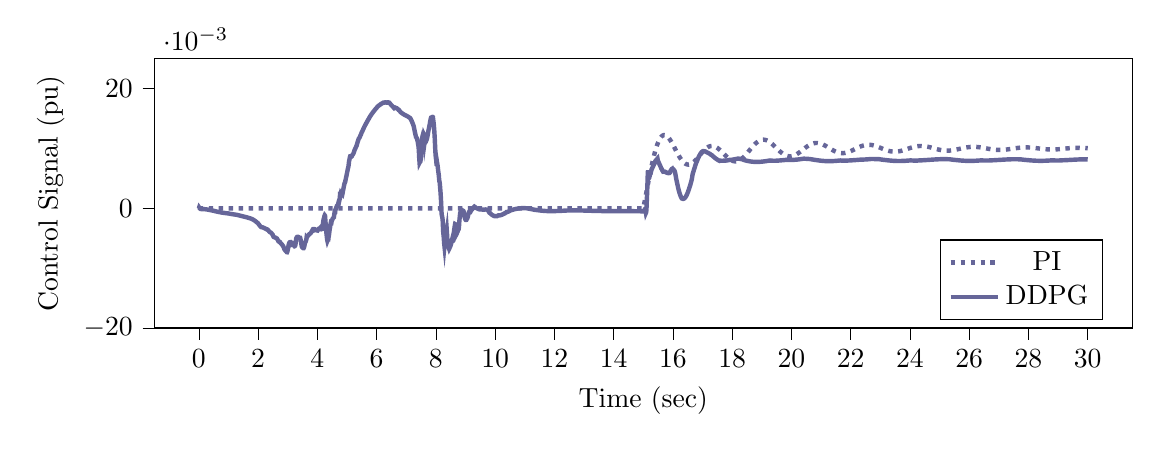
\begin{tikzpicture}

\definecolor{color0}{rgb}{0.12156862745098,0.466666666666667,0.705882352941177}
\definecolor{color1}{rgb}{1,0.498039215686275,0.0549019607843137}

\begin{axis}[
compat=newest,
tick align=outside,
tick pos=left,
x grid style={white!69.0196078431373!black},
xmin=-1.50000000000009, xmax=31.500000000002,
xtick style={color=black},
y grid style={white!69.0196078431373!black},
ymin=-0.02, ymax=0.025,
ytick style={color=black},
%yticklabel style={
%        /pgf/number format/.cd,
%        	fixed,
%        	fixed zerofill,
%         	precision=3,
%        /tikz/.cd
%},
scaled y ticks=true,
scaled y ticks=base 10:3,
width=14cm,
height=5cm,
xlabel=Time (sec),
ylabel=Control Signal (pu),
%y label style={at={(-0.2,0.5)}}
legend pos=south east
]

\addplot [ultra thick, blue!20!gray, dotted]
table {%
0 0
0.01 0
0.02 0
0.03 0
0.04 0
0.05 0
0.06 0
0.07 0
0.08 0
0.09 0
0.1 0
0.11 0
0.12 0
0.13 0
0.14 0
0.15 0
0.16 0
0.17 0
0.18 0
0.19 0
0.2 0
0.21 0
0.22 0
0.23 0
0.24 0
0.25 0
0.26 0
0.27 0
0.28 0
0.29 0
0.3 0
0.31 0
0.32 0
0.33 0
0.34 0
0.35 0
0.36 0
0.37 0
0.38 0
0.39 0
0.4 0
0.41 0
0.42 0
0.43 0
0.44 0
0.45 0
0.46 0
0.47 0
0.48 0
0.49 0
0.5 0
0.51 0
0.52 0
0.53 0
0.54 0
0.55 0
0.56 0
0.57 0
0.58 0
0.59 0
0.6 0
0.61 0
0.62 0
0.63 0
0.64 0
0.65 0
0.66 0
0.67 0
0.68 0
0.69 0
0.7 0
0.71 0
0.72 0
0.73 0
0.74 0
0.75 0
0.76 0
0.77 0
0.78 0
0.79 0
0.8 0
0.81 0
0.820000000000001 0
0.830000000000001 0
0.840000000000001 0
0.850000000000001 0
0.860000000000001 0
0.870000000000001 0
0.880000000000001 0
0.890000000000001 0
0.900000000000001 0
0.910000000000001 0
0.920000000000001 0
0.930000000000001 0
0.940000000000001 0
0.950000000000001 0
0.960000000000001 0
0.970000000000001 0
0.980000000000001 0
0.990000000000001 0
1 0
1.01 0
1.02 0
1.03 0
1.04 0
1.05 0
1.06 0
1.07 0
1.08 0
1.09 0
1.1 0
1.11 0
1.12 0
1.13 0
1.14 0
1.15 0
1.16 0
1.17 0
1.18 0
1.19 0
1.2 0
1.21 0
1.22 0
1.23 0
1.24 0
1.25 0
1.26 0
1.27 0
1.28 0
1.29 0
1.3 0
1.31 0
1.32 0
1.33 0
1.34 0
1.35 0
1.36 0
1.37 0
1.38 0
1.39 0
1.4 0
1.41 0
1.42 0
1.43 0
1.44 0
1.45 0
1.46 0
1.47 0
1.48 0
1.49 0
1.5 0
1.51 0
1.52 0
1.53 0
1.54 0
1.55 0
1.56 0
1.57 0
1.58 0
1.59 0
1.6 0
1.61 0
1.62 0
1.63 0
1.64 0
1.65 0
1.66 0
1.67 0
1.68 0
1.69 0
1.7 0
1.71 0
1.72 0
1.73 0
1.74 0
1.75 0
1.76 0
1.77 0
1.78 0
1.79 0
1.8 0
1.81 0
1.82 0
1.83 0
1.84 0
1.85 0
1.86 0
1.87 0
1.88 0
1.89 0
1.9 0
1.91 0
1.92 0
1.93 0
1.94 0
1.95 0
1.96 0
1.97 0
1.98 0
1.99 0
2 0
2.01 0
2.02 0
2.03 0
2.04 0
2.05 0
2.06 0
2.07 0
2.08 0
2.09 0
2.1 0
2.11 0
2.12 0
2.13 0
2.14 0
2.15 0
2.16 0
2.17 0
2.18 0
2.19 0
2.2 0
2.21 0
2.22 0
2.23 0
2.24 0
2.25 0
2.26 0
2.27 0
2.28 0
2.29 0
2.29999999999999 0
2.30999999999999 0
2.31999999999999 0
2.32999999999999 0
2.33999999999999 0
2.34999999999999 0
2.35999999999999 0
2.36999999999999 0
2.37999999999999 0
2.38999999999999 0
2.39999999999999 0
2.40999999999999 0
2.41999999999999 0
2.42999999999999 0
2.43999999999999 0
2.44999999999999 0
2.45999999999999 0
2.46999999999999 0
2.47999999999999 0
2.48999999999999 0
2.49999999999999 0
2.50999999999999 0
2.51999999999999 0
2.52999999999999 0
2.53999999999999 0
2.54999999999999 0
2.55999999999999 0
2.56999999999999 0
2.57999999999999 0
2.58999999999999 0
2.59999999999999 0
2.60999999999999 0
2.61999999999999 0
2.62999999999999 0
2.63999999999999 0
2.64999999999999 0
2.65999999999999 0
2.66999999999999 0
2.67999999999999 0
2.68999999999999 0
2.69999999999999 0
2.70999999999999 0
2.71999999999999 0
2.72999999999999 0
2.73999999999999 0
2.74999999999999 0
2.75999999999999 0
2.76999999999998 0
2.77999999999998 0
2.78999999999998 0
2.79999999999998 0
2.80999999999998 0
2.81999999999998 0
2.82999999999998 0
2.83999999999998 0
2.84999999999998 0
2.85999999999998 0
2.86999999999998 0
2.87999999999998 0
2.88999999999998 0
2.89999999999998 0
2.90999999999998 0
2.91999999999998 0
2.92999999999998 0
2.93999999999998 0
2.94999999999998 0
2.95999999999998 0
2.96999999999998 0
2.97999999999998 0
2.98999999999998 0
2.99999999999998 0
3.00999999999998 0
3.01999999999998 0
3.02999999999998 0
3.03999999999998 0
3.04999999999998 0
3.05999999999998 0
3.06999999999998 0
3.07999999999998 0
3.08999999999998 0
3.09999999999998 0
3.10999999999998 0
3.11999999999998 0
3.12999999999998 0
3.13999999999998 0
3.14999999999998 0
3.15999999999998 0
3.16999999999998 0
3.17999999999998 0
3.18999999999998 0
3.19999999999998 0
3.20999999999998 0
3.21999999999998 0
3.22999999999998 0
3.23999999999997 0
3.24999999999997 0
3.25999999999997 0
3.26999999999997 0
3.27999999999997 0
3.28999999999997 0
3.29999999999997 0
3.30999999999997 0
3.31999999999997 0
3.32999999999997 0
3.33999999999997 0
3.34999999999997 0
3.35999999999997 0
3.36999999999997 0
3.37999999999997 0
3.38999999999997 0
3.39999999999997 0
3.40999999999997 0
3.41999999999997 0
3.42999999999997 0
3.43999999999997 0
3.44999999999997 0
3.45999999999997 0
3.46999999999997 0
3.47999999999997 0
3.48999999999997 0
3.49999999999997 0
3.50999999999997 0
3.51999999999997 0
3.52999999999997 0
3.53999999999997 0
3.54999999999997 0
3.55999999999997 0
3.56999999999997 0
3.57999999999997 0
3.58999999999997 0
3.59999999999997 0
3.60999999999997 0
3.61999999999997 0
3.62999999999997 0
3.63999999999997 0
3.64999999999997 0
3.65999999999997 0
3.66999999999997 0
3.67999999999997 0
3.68999999999997 0
3.69999999999997 0
3.70999999999996 0
3.71999999999996 0
3.72999999999996 0
3.73999999999996 0
3.74999999999996 0
3.75999999999996 0
3.76999999999996 0
3.77999999999996 0
3.78999999999996 0
3.79999999999996 0
3.80999999999996 0
3.81999999999996 0
3.82999999999996 0
3.83999999999996 0
3.84999999999996 0
3.85999999999996 0
3.86999999999996 0
3.87999999999996 0
3.88999999999996 0
3.89999999999996 0
3.90999999999996 0
3.91999999999996 0
3.92999999999996 0
3.93999999999996 0
3.94999999999996 0
3.95999999999996 0
3.96999999999996 0
3.97999999999996 0
3.98999999999996 0
3.99999999999996 0
4.00999999999996 0
4.01999999999996 0
4.02999999999996 0
4.03999999999996 0
4.04999999999996 0
4.05999999999996 0
4.06999999999996 0
4.07999999999996 0
4.08999999999996 0
4.09999999999996 0
4.10999999999996 0
4.11999999999996 0
4.12999999999996 0
4.13999999999996 0
4.14999999999996 0
4.15999999999996 0
4.16999999999996 0
4.17999999999996 0
4.18999999999996 0
4.19999999999995 0
4.20999999999995 0
4.21999999999995 0
4.22999999999995 0
4.23999999999995 0
4.24999999999995 0
4.25999999999995 0
4.26999999999995 0
4.27999999999995 0
4.28999999999995 0
4.29999999999995 0
4.30999999999995 0
4.31999999999995 0
4.32999999999995 0
4.33999999999995 0
4.34999999999995 0
4.35999999999995 0
4.36999999999995 0
4.37999999999995 0
4.38999999999995 0
4.39999999999995 0
4.40999999999995 0
4.41999999999995 0
4.42999999999995 0
4.43999999999995 0
4.44999999999995 0
4.45999999999995 0
4.46999999999995 0
4.47999999999995 0
4.48999999999995 0
4.49999999999995 0
4.50999999999995 0
4.51999999999995 0
4.52999999999995 0
4.53999999999995 0
4.54999999999995 0
4.55999999999995 0
4.56999999999995 0
4.57999999999995 0
4.58999999999995 0
4.59999999999995 0
4.60999999999995 0
4.61999999999995 0
4.62999999999995 0
4.63999999999995 0
4.64999999999995 0
4.65999999999995 0
4.66999999999994 0
4.67999999999994 0
4.68999999999994 0
4.69999999999994 0
4.70999999999994 0
4.71999999999994 0
4.72999999999994 0
4.73999999999994 0
4.74999999999994 0
4.75999999999994 0
4.76999999999994 0
4.77999999999994 0
4.78999999999994 0
4.79999999999994 0
4.80999999999994 0
4.81999999999994 0
4.82999999999994 0
4.83999999999994 0
4.84999999999994 0
4.85999999999994 0
4.86999999999994 0
4.87999999999994 0
4.88999999999994 0
4.89999999999994 0
4.90999999999994 0
4.91999999999994 0
4.92999999999994 0
4.93999999999994 0
4.94999999999994 0
4.95999999999994 0
4.96999999999994 0
4.97999999999994 0
4.98999999999994 0
4.99999999999994 0
5.00999999999994 0
5.01999999999994 0
5.02999999999994 0
5.03999999999994 0
5.04999999999994 0
5.05999999999994 0
5.06999999999994 0
5.07999999999994 0
5.08999999999994 0
5.09999999999994 0
5.10999999999994 0
5.11999999999994 0
5.12999999999994 0
5.13999999999993 0
5.14999999999993 0
5.15999999999993 0
5.16999999999993 0
5.17999999999993 0
5.18999999999993 0
5.19999999999993 0
5.20999999999993 0
5.21999999999993 0
5.22999999999993 0
5.23999999999993 0
5.24999999999993 0
5.25999999999993 0
5.26999999999993 0
5.27999999999993 0
5.28999999999993 0
5.29999999999993 0
5.30999999999993 0
5.31999999999993 0
5.32999999999993 0
5.33999999999993 0
5.34999999999993 0
5.35999999999993 0
5.36999999999993 0
5.37999999999993 0
5.38999999999993 0
5.39999999999993 0
5.40999999999993 0
5.41999999999993 0
5.42999999999993 0
5.43999999999993 0
5.44999999999993 0
5.45999999999993 0
5.46999999999993 0
5.47999999999993 0
5.48999999999993 0
5.49999999999993 0
5.50999999999993 0
5.51999999999993 0
5.52999999999993 0
5.53999999999993 0
5.54999999999993 0
5.55999999999993 0
5.56999999999993 0
5.57999999999993 0
5.58999999999993 0
5.59999999999993 0
5.60999999999992 0
5.61999999999992 0
5.62999999999992 0
5.63999999999992 0
5.64999999999992 0
5.65999999999992 0
5.66999999999992 0
5.67999999999992 0
5.68999999999992 0
5.69999999999992 0
5.70999999999992 0
5.71999999999992 0
5.72999999999992 0
5.73999999999992 0
5.74999999999992 0
5.75999999999992 0
5.76999999999992 0
5.77999999999992 0
5.78999999999992 0
5.79999999999992 0
5.80999999999992 0
5.81999999999992 0
5.82999999999992 0
5.83999999999992 0
5.84999999999992 0
5.85999999999992 0
5.86999999999992 0
5.87999999999992 0
5.88999999999992 0
5.89999999999992 0
5.90999999999992 0
5.91999999999992 0
5.92999999999992 0
5.93999999999992 0
5.94999999999992 0
5.95999999999992 0
5.96999999999992 0
5.97999999999992 0
5.98999999999992 0
5.99999999999992 0
6.00999999999992 0
6.01999999999992 0
6.02999999999992 0
6.03999999999992 0
6.04999999999992 0
6.05999999999992 0
6.06999999999992 0
6.07999999999991 0
6.08999999999991 0
6.09999999999991 0
6.10999999999991 0
6.11999999999991 0
6.12999999999991 0
6.13999999999991 0
6.14999999999991 0
6.15999999999991 0
6.16999999999991 0
6.17999999999991 0
6.18999999999991 0
6.19999999999991 0
6.20999999999991 0
6.21999999999991 0
6.22999999999991 0
6.23999999999991 0
6.24999999999991 0
6.25999999999991 0
6.26999999999991 0
6.27999999999991 0
6.28999999999991 0
6.29999999999991 0
6.30999999999991 0
6.31999999999991 0
6.32999999999991 0
6.33999999999991 0
6.34999999999991 0
6.35999999999991 0
6.36999999999991 0
6.37999999999991 0
6.38999999999991 0
6.39999999999991 0
6.40999999999991 0
6.41999999999991 0
6.42999999999991 0
6.43999999999991 0
6.44999999999991 0
6.45999999999991 0
6.46999999999991 0
6.47999999999991 0
6.48999999999991 0
6.49999999999991 0
6.50999999999991 0
6.51999999999991 0
6.52999999999991 0
6.53999999999991 0
6.5499999999999 0
6.5599999999999 0
6.5699999999999 0
6.5799999999999 0
6.5899999999999 0
6.5999999999999 0
6.6099999999999 0
6.6199999999999 0
6.6299999999999 0
6.6399999999999 0
6.6499999999999 0
6.6599999999999 0
6.6699999999999 0
6.6799999999999 0
6.6899999999999 0
6.6999999999999 0
6.7099999999999 0
6.7199999999999 0
6.7299999999999 0
6.7399999999999 0
6.7499999999999 0
6.7599999999999 0
6.7699999999999 0
6.7799999999999 0
6.7899999999999 0
6.7999999999999 0
6.8099999999999 0
6.8199999999999 0
6.8299999999999 0
6.8399999999999 0
6.8499999999999 0
6.8599999999999 0
6.8699999999999 0
6.8799999999999 0
6.8899999999999 0
6.8999999999999 0
6.9099999999999 0
6.9199999999999 0
6.9299999999999 0
6.9399999999999 0
6.9499999999999 0
6.9599999999999 0
6.9699999999999 0
6.9799999999999 0
6.9899999999999 0
6.9999999999999 0
7.00999999999989 0
7.01999999999989 0
7.02999999999989 0
7.03999999999989 0
7.04999999999989 0
7.05999999999989 0
7.06999999999989 0
7.07999999999989 0
7.08999999999989 0
7.09999999999989 0
7.10999999999989 0
7.11999999999989 0
7.12999999999989 0
7.13999999999989 0
7.14999999999989 0
7.15999999999989 0
7.16999999999989 0
7.17999999999989 0
7.18999999999989 0
7.19999999999989 0
7.20999999999989 0
7.21999999999989 0
7.22999999999989 0
7.23999999999989 0
7.24999999999989 0
7.25999999999989 0
7.26999999999989 0
7.27999999999989 0
7.28999999999989 0
7.29999999999989 0
7.30999999999989 0
7.31999999999989 0
7.32999999999989 0
7.33999999999989 0
7.34999999999989 0
7.35999999999989 0
7.36999999999989 0
7.37999999999989 0
7.38999999999989 0
7.39999999999989 0
7.40999999999989 0
7.41999999999989 0
7.42999999999989 0
7.43999999999989 0
7.44999999999989 0
7.45999999999989 0
7.46999999999989 0
7.47999999999988 0
7.48999999999988 0
7.49999999999988 0
7.50999999999988 0
7.51999999999988 0
7.52999999999988 0
7.53999999999988 0
7.54999999999988 0
7.55999999999988 0
7.56999999999988 0
7.57999999999988 0
7.58999999999988 0
7.59999999999988 0
7.60999999999988 0
7.61999999999988 0
7.62999999999988 0
7.63999999999988 0
7.64999999999988 0
7.65999999999988 0
7.66999999999988 0
7.67999999999988 0
7.68999999999988 0
7.69999999999988 0
7.70999999999988 0
7.71999999999988 0
7.72999999999988 0
7.73999999999988 0
7.74999999999988 0
7.75999999999988 0
7.76999999999988 0
7.77999999999988 0
7.78999999999988 0
7.79999999999988 0
7.80999999999988 0
7.81999999999988 0
7.82999999999988 0
7.83999999999988 0
7.84999999999988 0
7.85999999999988 0
7.86999999999988 0
7.87999999999988 0
7.88999999999988 0
7.89999999999988 0
7.90999999999988 0
7.91999999999988 0
7.92999999999988 0
7.93999999999988 0
7.94999999999987 0
7.95999999999987 0
7.96999999999987 0
7.97999999999987 0
7.98999999999987 0
7.99999999999987 0
8.00999999999987 0
8.01999999999987 0
8.02999999999987 0
8.03999999999987 0
8.04999999999987 0
8.05999999999987 0
8.06999999999987 0
8.07999999999987 0
8.08999999999987 0
8.09999999999987 0
8.10999999999987 0
8.11999999999987 0
8.12999999999987 0
8.13999999999987 0
8.14999999999987 0
8.15999999999987 0
8.16999999999987 0
8.17999999999987 0
8.18999999999987 0
8.19999999999987 0
8.20999999999987 0
8.21999999999987 0
8.22999999999987 0
8.23999999999987 0
8.24999999999987 0
8.25999999999987 0
8.26999999999987 0
8.27999999999987 0
8.28999999999987 0
8.29999999999987 0
8.30999999999987 0
8.31999999999987 0
8.32999999999987 0
8.33999999999987 0
8.34999999999987 0
8.35999999999987 0
8.36999999999987 0
8.37999999999987 0
8.38999999999987 0
8.39999999999987 0
8.40999999999987 0
8.41999999999986 0
8.42999999999986 0
8.43999999999986 0
8.44999999999986 0
8.45999999999986 0
8.46999999999986 0
8.47999999999986 0
8.48999999999986 0
8.49999999999986 0
8.50999999999986 0
8.51999999999986 0
8.52999999999986 0
8.53999999999986 0
8.54999999999986 0
8.55999999999986 0
8.56999999999986 0
8.57999999999986 0
8.58999999999986 0
8.59999999999986 0
8.60999999999986 0
8.61999999999986 0
8.62999999999986 0
8.63999999999986 0
8.64999999999986 0
8.65999999999986 0
8.66999999999986 0
8.67999999999986 0
8.68999999999986 0
8.69999999999986 0
8.70999999999986 0
8.71999999999986 0
8.72999999999986 0
8.73999999999986 0
8.74999999999986 0
8.75999999999986 0
8.76999999999986 0
8.77999999999986 0
8.78999999999986 0
8.79999999999986 0
8.80999999999986 0
8.81999999999986 0
8.82999999999986 0
8.83999999999986 0
8.84999999999986 0
8.85999999999986 0
8.86999999999986 0
8.87999999999986 0
8.88999999999985 0
8.89999999999985 0
8.90999999999985 0
8.91999999999985 0
8.92999999999985 0
8.93999999999985 0
8.94999999999985 0
8.95999999999985 0
8.96999999999985 0
8.97999999999985 0
8.98999999999985 0
8.99999999999985 0
9.00999999999985 0
9.01999999999985 0
9.02999999999985 0
9.03999999999985 0
9.04999999999985 0
9.05999999999985 0
9.06999999999985 0
9.07999999999985 0
9.08999999999985 0
9.09999999999985 0
9.10999999999985 0
9.11999999999985 0
9.12999999999985 0
9.13999999999985 0
9.14999999999985 0
9.15999999999985 0
9.16999999999985 0
9.17999999999985 0
9.18999999999985 0
9.19999999999985 0
9.20999999999985 0
9.21999999999985 0
9.22999999999985 0
9.23999999999985 0
9.24999999999985 0
9.25999999999985 0
9.26999999999985 0
9.27999999999985 0
9.28999999999985 0
9.29999999999985 0
9.30999999999985 0
9.31999999999985 0
9.32999999999985 0
9.33999999999985 0
9.34999999999985 0
9.35999999999984 0
9.36999999999984 0
9.37999999999984 0
9.38999999999984 0
9.39999999999984 0
9.40999999999984 0
9.41999999999984 0
9.42999999999984 0
9.43999999999984 0
9.44999999999984 0
9.45999999999984 0
9.46999999999984 0
9.47999999999984 0
9.48999999999984 0
9.49999999999984 0
9.50999999999984 0
9.51999999999984 0
9.52999999999984 0
9.53999999999984 0
9.54999999999984 0
9.55999999999984 0
9.56999999999984 0
9.57999999999984 0
9.58999999999984 0
9.59999999999984 0
9.60999999999984 0
9.61999999999984 0
9.62999999999984 0
9.63999999999984 0
9.64999999999984 0
9.65999999999984 0
9.66999999999984 0
9.67999999999984 0
9.68999999999984 0
9.69999999999984 0
9.70999999999984 0
9.71999999999984 0
9.72999999999984 0
9.73999999999984 0
9.74999999999984 0
9.75999999999984 0
9.76999999999984 0
9.77999999999984 0
9.78999999999984 0
9.79999999999984 0
9.80999999999984 0
9.81999999999984 0
9.82999999999983 0
9.83999999999983 0
9.84999999999983 0
9.85999999999983 0
9.86999999999983 0
9.87999999999983 0
9.88999999999983 0
9.89999999999983 0
9.90999999999983 0
9.91999999999983 0
9.92999999999983 0
9.93999999999983 0
9.94999999999983 0
9.95999999999983 0
9.96999999999983 0
9.97999999999983 0
9.98999999999983 0
9.99999999999983 0
10.0099999999998 0
10.0199999999998 0
10.0299999999998 0
10.0399999999998 0
10.0499999999998 0
10.0599999999998 0
10.0699999999998 0
10.0799999999998 0
10.0899999999998 0
10.0999999999998 0
10.1099999999998 0
10.1199999999998 0
10.1299999999998 0
10.1399999999998 0
10.1499999999998 0
10.1599999999998 0
10.1699999999998 0
10.1799999999998 0
10.1899999999998 0
10.1999999999998 0
10.2099999999998 0
10.2199999999998 0
10.2299999999998 0
10.2399999999998 0
10.2499999999998 0
10.2599999999998 0
10.2699999999998 0
10.2799999999998 0
10.2899999999998 0
10.2999999999998 0
10.3099999999998 0
10.3199999999998 0
10.3299999999998 0
10.3399999999998 0
10.3499999999998 0
10.3599999999998 0
10.3699999999998 0
10.3799999999998 0
10.3899999999998 0
10.3999999999998 0
10.4099999999998 0
10.4199999999998 0
10.4299999999998 0
10.4399999999998 0
10.4499999999998 0
10.4599999999998 0
10.4699999999998 0
10.4799999999998 0
10.4899999999998 0
10.4999999999998 0
10.5099999999998 0
10.5199999999998 0
10.5299999999998 0
10.5399999999998 0
10.5499999999998 0
10.5599999999998 0
10.5699999999998 0
10.5799999999998 0
10.5899999999998 0
10.5999999999998 0
10.6099999999998 0
10.6199999999998 0
10.6299999999998 0
10.6399999999998 0
10.6499999999998 0
10.6599999999998 0
10.6699999999998 0
10.6799999999998 0
10.6899999999998 0
10.6999999999998 0
10.7099999999998 0
10.7199999999998 0
10.7299999999998 0
10.7399999999998 0
10.7499999999998 0
10.7599999999998 0
10.7699999999998 0
10.7799999999998 0
10.7899999999998 0
10.7999999999998 0
10.8099999999998 0
10.8199999999998 0
10.8299999999998 0
10.8399999999998 0
10.8499999999998 0
10.8599999999998 0
10.8699999999998 0
10.8799999999998 0
10.8899999999998 0
10.8999999999998 0
10.9099999999998 0
10.9199999999998 0
10.9299999999998 0
10.9399999999998 0
10.9499999999998 0
10.9599999999998 0
10.9699999999998 0
10.9799999999998 0
10.9899999999998 0
10.9999999999998 0
11.0099999999998 0
11.0199999999998 0
11.0299999999998 0
11.0399999999998 0
11.0499999999998 0
11.0599999999998 0
11.0699999999998 0
11.0799999999998 0
11.0899999999998 0
11.0999999999998 0
11.1099999999998 0
11.1199999999998 0
11.1299999999998 0
11.1399999999998 0
11.1499999999998 0
11.1599999999998 0
11.1699999999998 0
11.1799999999998 0
11.1899999999998 0
11.1999999999998 0
11.2099999999998 0
11.2199999999998 0
11.2299999999998 0
11.2399999999998 0
11.2499999999998 0
11.2599999999998 0
11.2699999999998 0
11.2799999999998 0
11.2899999999998 0
11.2999999999998 0
11.3099999999998 0
11.3199999999998 0
11.3299999999998 0
11.3399999999998 0
11.3499999999998 0
11.3599999999998 0
11.3699999999998 0
11.3799999999998 0
11.3899999999998 0
11.3999999999998 0
11.4099999999998 0
11.4199999999998 0
11.4299999999998 0
11.4399999999998 0
11.4499999999998 0
11.4599999999998 0
11.4699999999998 0
11.4799999999998 0
11.4899999999998 0
11.4999999999998 0
11.5099999999998 0
11.5199999999998 0
11.5299999999998 0
11.5399999999998 0
11.5499999999998 0
11.5599999999998 0
11.5699999999998 0
11.5799999999998 0
11.5899999999998 0
11.5999999999998 0
11.6099999999998 0
11.6199999999998 0
11.6299999999998 0
11.6399999999998 0
11.6499999999998 0
11.6599999999998 0
11.6699999999998 0
11.6799999999998 0
11.6899999999998 0
11.6999999999998 0
11.7099999999998 0
11.7199999999998 0
11.7299999999998 0
11.7399999999998 0
11.7499999999998 0
11.7599999999998 0
11.7699999999998 0
11.7799999999998 0
11.7899999999998 0
11.7999999999998 0
11.8099999999998 0
11.8199999999998 0
11.8299999999998 0
11.8399999999998 0
11.8499999999998 0
11.8599999999998 0
11.8699999999998 0
11.8799999999998 0
11.8899999999998 0
11.8999999999998 0
11.9099999999998 0
11.9199999999998 0
11.9299999999998 0
11.9399999999998 0
11.9499999999998 0
11.9599999999998 0
11.9699999999998 0
11.9799999999998 0
11.9899999999998 0
11.9999999999998 0
12.0099999999998 0
12.0199999999998 0
12.0299999999998 0
12.0399999999998 0
12.0499999999998 0
12.0599999999998 0
12.0699999999998 0
12.0799999999998 0
12.0899999999998 0
12.0999999999998 0
12.1099999999998 0
12.1199999999998 0
12.1299999999998 0
12.1399999999998 0
12.1499999999998 0
12.1599999999998 0
12.1699999999998 0
12.1799999999998 0
12.1899999999998 0
12.1999999999998 0
12.2099999999998 0
12.2199999999998 0
12.2299999999998 0
12.2399999999998 0
12.2499999999998 0
12.2599999999998 0
12.2699999999998 0
12.2799999999998 0
12.2899999999998 0
12.2999999999998 0
12.3099999999998 0
12.3199999999998 0
12.3299999999998 0
12.3399999999998 0
12.3499999999998 0
12.3599999999998 0
12.3699999999998 0
12.3799999999998 0
12.3899999999998 0
12.3999999999998 0
12.4099999999998 0
12.4199999999998 0
12.4299999999998 0
12.4399999999998 0
12.4499999999998 0
12.4599999999998 0
12.4699999999998 0
12.4799999999998 0
12.4899999999998 0
12.4999999999998 0
12.5099999999998 0
12.5199999999998 0
12.5299999999998 0
12.5399999999998 0
12.5499999999998 0
12.5599999999998 0
12.5699999999998 0
12.5799999999998 0
12.5899999999998 0
12.5999999999998 0
12.6099999999998 0
12.6199999999998 0
12.6299999999998 0
12.6399999999998 0
12.6499999999998 0
12.6599999999998 0
12.6699999999998 0
12.6799999999998 0
12.6899999999998 0
12.6999999999998 0
12.7099999999998 0
12.7199999999998 0
12.7299999999998 0
12.7399999999998 0
12.7499999999998 0
12.7599999999998 0
12.7699999999998 0
12.7799999999998 0
12.7899999999998 0
12.7999999999998 0
12.8099999999998 0
12.8199999999998 0
12.8299999999998 0
12.8399999999998 0
12.8499999999998 0
12.8599999999998 0
12.8699999999998 0
12.8799999999998 0
12.8899999999998 0
12.8999999999998 0
12.9099999999998 0
12.9199999999998 0
12.9299999999998 0
12.9399999999998 0
12.9499999999998 0
12.9599999999998 0
12.9699999999998 0
12.9799999999998 0
12.9899999999998 0
12.9999999999998 0
13.0099999999998 0
13.0199999999998 0
13.0299999999998 0
13.0399999999998 0
13.0499999999998 0
13.0599999999998 0
13.0699999999998 0
13.0799999999998 0
13.0899999999998 0
13.0999999999998 0
13.1099999999998 0
13.1199999999998 0
13.1299999999998 0
13.1399999999998 0
13.1499999999998 0
13.1599999999998 0
13.1699999999998 0
13.1799999999998 0
13.1899999999998 0
13.1999999999998 0
13.2099999999998 0
13.2199999999998 0
13.2299999999998 0
13.2399999999998 0
13.2499999999998 0
13.2599999999998 0
13.2699999999998 0
13.2799999999998 0
13.2899999999998 0
13.2999999999998 0
13.3099999999998 0
13.3199999999998 0
13.3299999999998 0
13.3399999999998 0
13.3499999999998 0
13.3599999999998 0
13.3699999999998 0
13.3799999999998 0
13.3899999999998 0
13.3999999999998 0
13.4099999999998 0
13.4199999999998 0
13.4299999999998 0
13.4399999999998 0
13.4499999999998 0
13.4599999999998 0
13.4699999999998 0
13.4799999999998 0
13.4899999999998 0
13.4999999999998 0
13.5099999999998 0
13.5199999999998 0
13.5299999999998 0
13.5399999999998 0
13.5499999999998 0
13.5599999999998 0
13.5699999999998 0
13.5799999999998 0
13.5899999999998 0
13.5999999999998 0
13.6099999999998 0
13.6199999999998 0
13.6299999999998 0
13.6399999999998 0
13.6499999999998 0
13.6599999999998 0
13.6699999999998 0
13.6799999999998 0
13.6899999999998 0
13.6999999999998 0
13.7099999999998 0
13.7199999999998 0
13.7299999999998 0
13.7399999999998 0
13.7499999999998 0
13.7599999999998 0
13.7699999999998 0
13.7799999999998 0
13.7899999999998 0
13.7999999999998 0
13.8099999999998 0
13.8199999999997 0
13.8299999999997 0
13.8399999999997 0
13.8499999999997 0
13.8599999999997 0
13.8699999999997 0
13.8799999999997 0
13.8899999999997 0
13.8999999999997 0
13.9099999999997 0
13.9199999999997 0
13.9299999999997 0
13.9399999999997 0
13.9499999999997 0
13.9599999999997 0
13.9699999999997 0
13.9799999999997 0
13.9899999999997 0
13.9999999999997 0
14.0099999999997 0
14.0199999999997 0
14.0299999999997 0
14.0399999999997 0
14.0499999999997 0
14.0599999999997 0
14.0699999999997 0
14.0799999999997 0
14.0899999999997 0
14.0999999999997 0
14.1099999999997 0
14.1199999999997 0
14.1299999999997 0
14.1399999999997 0
14.1499999999997 0
14.1599999999997 0
14.1699999999997 0
14.1799999999997 0
14.1899999999997 0
14.1999999999997 0
14.2099999999997 0
14.2199999999997 0
14.2299999999997 0
14.2399999999997 0
14.2499999999997 0
14.2599999999997 0
14.2699999999997 0
14.2799999999997 0
14.2899999999997 0
14.2999999999997 0
14.3099999999997 0
14.3199999999997 0
14.3299999999997 0
14.3399999999997 0
14.3499999999997 0
14.3599999999997 0
14.3699999999997 0
14.3799999999997 0
14.3899999999997 0
14.3999999999997 0
14.4099999999997 0
14.4199999999997 0
14.4299999999997 0
14.4399999999997 0
14.4499999999997 0
14.4599999999997 0
14.4699999999997 0
14.4799999999997 0
14.4899999999997 0
14.4999999999997 0
14.5099999999997 0
14.5199999999997 0
14.5299999999997 0
14.5399999999997 0
14.5499999999997 0
14.5599999999997 0
14.5699999999997 0
14.5799999999997 0
14.5899999999997 0
14.5999999999997 0
14.6099999999997 0
14.6199999999997 0
14.6299999999997 0
14.6399999999997 0
14.6499999999997 0
14.6599999999997 0
14.6699999999997 0
14.6799999999997 0
14.6899999999997 0
14.6999999999997 0
14.7099999999997 0
14.7199999999997 0
14.7299999999997 0
14.7399999999997 0
14.7499999999997 0
14.7599999999997 0
14.7699999999997 0
14.7799999999997 0
14.7899999999997 0
14.7999999999997 0
14.8099999999997 0
14.8199999999997 0
14.8299999999997 0
14.8399999999997 0
14.8499999999997 0
14.8599999999997 0
14.8699999999997 0
14.8799999999997 0
14.8899999999997 0
14.8999999999997 0
14.9099999999997 0
14.9199999999997 0
14.9299999999997 0
14.9399999999997 0
14.9499999999997 0
14.9599999999997 0
14.9699999999997 0
14.9799999999997 0
14.9899999999997 0
14.9999999999997 1.65143933586237e-09
15.0099999999997 0.000251646628705991
15.0199999999997 0.000504813715529082
15.0299999999997 0.000759409495223724
15.0399999999997 0.0010153171453592
15.0499999999997 0.00127240160730084
15.0599999999997 0.00153051202950275
15.0699999999997 0.0017894842012412
15.0799999999997 0.00204914261052369
15.0899999999997 0.00230930228873294
15.0999999999997 0.00256977047864943
15.1099999999997 0.00283034812071255
15.1199999999997 0.00309083117851801
15.1299999999997 0.00335101182327691
15.1399999999997 0.00361067949426346
15.1499999999997 0.00386962185004272
15.1599999999997 0.00412762562336092
15.1699999999997 0.00438447739093926
15.1799999999997 0.00463996426797917
15.1899999999997 0.0048938745359416
15.1999999999997 0.00514599821107789
15.2099999999997 0.00539612756023699
15.2199999999997 0.00564405756964693
15.2299999999997 0.0058895863716423
15.2399999999997 0.00613251563367615
15.2499999999997 0.00637265091340354
15.2599999999997 0.0066098019831371
15.2699999999997 0.00684378312655668
15.2799999999997 0.00707441341018548
15.2899999999997 0.00730151693182289
15.2999999999997 0.00752492304784595
15.3099999999997 0.0077444665810465
15.3199999999997 0.00795998801045696
15.3299999999997 0.00817133364443574
15.3399999999997 0.0083783557781198
15.3499999999997 0.0085809128362127
15.3599999999997 0.00877886950195709
15.3699999999997 0.00897209683303236
15.3799999999997 0.00916047236503106
15.3899999999997 0.00934388020308567
15.3999999999997 0.0095222111021532
15.4099999999997 0.00969536253640429
15.4199999999997 0.00986323875811496
15.4299999999997 0.0100257508464171
15.4399999999997 0.010182816746761
15.4499999999997 0.0103343612993197
15.4599999999997 0.0104803162594725
15.4699999999997 0.0106206203089849
15.4799999999997 0.0107552190583435
15.4899999999997 0.0108840650409438
15.4999999999997 0.0110071176972975
15.5099999999997 0.011124343352648
15.5199999999997 0.0112357151860114
15.5299999999997 0.0113412131913552
15.5399999999997 0.0114408241310805
15.5499999999997 0.0115345414819743
15.5599999999997 0.0116223653737919
15.5699999999997 0.0117043025206279
15.5799999999997 0.0117803661451226
15.5899999999997 0.0118505758952864
15.5999999999997 0.0119149579143133
15.6099999999997 0.0119735446087437
15.6199999999997 0.0120263743730305
15.6299999999997 0.0120734916350397
15.6399999999997 0.0121149467423113
15.6499999999997 0.0121507958425362
15.6599999999997 0.0121811007584378
15.6699999999997 0.0122059288572524
15.6799999999997 0.0122253529150019
15.6899999999997 0.0122394509757588
15.6999999999997 0.0122483062073349
15.7099999999997 0.0122520067746912
15.7199999999997 0.0122506459870169
15.7299999999997 0.0122443214434493
15.7399999999997 0.0122331352385886
15.7499999999997 0.0122171937960714
15.7599999999997 0.0121966076985984
15.7699999999997 0.0121714915146394
15.7799999999997 0.0121419636227105
15.7899999999997 0.0121081460308243
15.7999999999997 0.0120701641950366
15.8099999999997 0.0120281468355185
15.8199999999997 0.0119822257500982
15.8299999999997 0.0119325356249662
15.8399999999997 0.0118792138450612
15.8499999999997 0.0118224003024289
15.8599999999997 0.0117622372033321
15.8699999999997 0.0116988688743441
15.8799999999997 0.0116324415676611
15.8899999999997 0.0115631032658651
15.8999999999997 0.0114910034863693
15.9099999999997 0.0114162930857789
15.9199999999997 0.0113391240643967
15.9299999999997 0.0112596493713743
15.9399999999997 0.0111780227107287
15.9499999999997 0.0110943983459273
15.9599999999997 0.0110089309081382
15.9699999999997 0.0109217752048475
15.9799999999997 0.0108330860299626
15.9899999999997 0.010743017975616
15.9999999999997 0.0106517252458821
16.0099999999997 0.0105593614726147
16.0199999999997 0.010466079533611
16.0299999999997 0.0103720313733037
16.0399999999997 0.0102773678261791
16.0499999999997 0.0101822384431166
16.0599999999997 0.0100867913207596
16.0699999999997 0.00999117282763884
16.0799999999997 0.00989552761682951
16.0899999999997 0.00979999839634916
16.0999999999997 0.009704725772254
16.1099999999997 0.00960984809572078
16.1199999999997 0.00951550131426175
16.1299999999997 0.00942181882721364
16.1399999999997 0.00932893134564011
16.1499999999997 0.00923696675677972
16.1599999999997 0.00914604999316607
16.1699999999997 0.00905630290654273
16.1799999999997 0.00896784414668765
16.1899999999997 0.00888078904525547
16.1999999999997 0.00879524950474298
16.2099999999997 0.00871133389267151
16.2199999999997 0.00862914694107768
16.2299999999997 0.00854878965139488
16.2399999999997 0.00847035920480175
16.2499999999997 0.00839394887810764
16.2599999999997 0.00831964796523675
16.2699999999997 0.00824754170436735
16.2799999999997 0.008177711210774
16.2899999999997 0.00811023341541516
16.2999999999997 0.00804518100930091
16.3099999999998 0.00798262239366929
16.3199999999998 0.00792262159736296
16.3299999999998 0.00786523821083156
16.3399999999998 0.00781052751081816
16.3499999999998 0.0077585403426363
16.3599999999998 0.00770932304518571
16.3699999999998 0.00766291745392498
16.3799999999998 0.00761936101587842
16.3899999999998 0.0075786866982003
16.3999999999998 0.00754092299039499
16.4099999999998 0.00750609391217645
16.4199999999998 0.00747421902746872
16.4299999999998 0.00744531346441154
16.4399999999998 0.00741938793560937
16.4499999999998 0.00739644877097179
16.4599999999998 0.00737649795300926
16.4699999999998 0.007359533157394
16.4799999999998 0.00734554780005938
16.4899999999998 0.00733453108596858
16.4999999999998 0.00732646806304129
16.5099999999998 0.00732133968568659
16.5199999999998 0.00731912288018435
16.5299999999998 0.00731979021864938
16.5399999999998 0.00732331066143274
16.5499999999998 0.00732964953970922
16.5599999999998 0.00733876845866182
16.5699999999998 0.00735062538578098
16.5799999999998 0.00736517474296724
16.5899999999998 0.00738236750233981
16.5999999999998 0.00740215128563695
16.6099999999998 0.00742447046708126
16.6199999999998 0.00744926627957387
16.6299999999998 0.00747647692407254
16.6399999999998 0.00750603768200355
16.6499999999998 0.00753788102880218
16.6599999999998 0.00757193675519417
16.6699999999998 0.00760813208638035
16.6799999999998 0.0076463918048768
16.6899999999998 0.00768663837567033
16.6999999999998 0.00772879207341752
16.7099999999998 0.00777277111151301
16.7199999999998 0.00781849177285081
16.7299999999998 0.00786586854210142
16.7399999999998 0.00791481423932581
16.7499999999998 0.00796524015474771
16.7599999999998 0.00801705618450379
16.7699999999998 0.00807017096719201
16.7799999999998 0.00812449202103842
16.7899999999998 0.00817992588150534
16.7999999999998 0.00823637823918295
16.8099999999998 0.00829375407769597
16.8199999999998 0.00835195781154313
16.8299999999998 0.00841089342367419
16.8399999999998 0.00847046460261877
16.8499999999998 0.00853057487899296
16.8599999999998 0.00859112776121231
16.8699999999998 0.00865202687024156
16.8799999999998 0.00871317607321355
16.8899999999998 0.00877447961575266
16.8999999999998 0.00883584225283994
16.9099999999998 0.00889716937806082
16.9199999999998 0.00895836715107769
16.9299999999998 0.00901934262317827
16.9399999999998 0.00908000386074412
16.9499999999999 0.00914026006649596
16.9599999999999 0.00920002169835777
16.9699999999999 0.00925920058579342
16.9799999999999 0.00931771004357101
16.9899999999999 0.00937546498272624
16.9999999999999 0.00943238201862552
17.0099999999999 0.00948837957600957
17.0199999999999 0.00954337799089992
17.0299999999999 0.00959729960925543
17.0399999999999 0.00965006888227058
17.0499999999999 0.00970161245821259
17.0599999999999 0.00975185927069889
17.0699999999999 0.00980074062332166
17.0799999999999 0.00984819027053153
17.0899999999999 0.00989414449469739
17.0999999999999 0.00993854217900834
17.1099999999999 0.00998132487436766
17.1199999999999 0.0100224368699089
17.1299999999999 0.0100618252514182
17.1399999999999 0.0100994399579998
17.1499999999999 0.0101352338347464
17.1599999999999 0.010169162681151
17.1699999999999 0.010201185295265
17.1799999999999 0.0102312635136516
17.1899999999999 0.0102593622462963
17.1999999999999 0.0102854495078829
17.2099999999999 0.0103094966656106
17.2199999999999 0.0103314780482327
17.2299999999999 0.0103513711504976
17.2399999999999 0.0103691566538226
17.2499999999999 0.0103848184356419
17.2599999999999 0.0103983435743842
17.2699999999999 0.0104097223501043
17.2799999999999 0.0104189482402235
17.2899999999999 0.0104260179116881
17.2999999999999 0.0104309312106239
17.3099999999999 0.010433691144361
17.3199999999999 0.0104343038608099
17.3299999999999 0.0104327786237182
17.3399999999999 0.0104291277838637
17.3499999999999 0.010423366746246
17.3599999999999 0.0104155139333574
17.3699999999999 0.0104055907445939
17.3799999999999 0.0103936215117882
17.3899999999999 0.0103796334511415
17.3999999999999 0.010363656611495
17.4099999999999 0.0103457238190677
17.4199999999999 0.0103258706187556
17.4299999999999 0.0103041352120879
17.4399999999999 0.0102805583919461
17.4499999999999 0.0102551834741514
17.4599999999999 0.0102280562260332
17.4699999999999 0.0101992247920941
17.4799999999999 0.0101687396168962
17.4899999999999 0.0101366533686173
17.4999999999999 0.0101030208546709
17.5099999999999 0.0100678989305911
17.5199999999999 0.010031346418222
17.5299999999999 0.00999342401676745
17.5399999999999 0.00995419442535841
17.5499999999999 0.00991372222207376
17.5599999999999 0.00987207301579076
17.5699999999999 0.00982931393566132
17.5799999999999 0.00978551352605559
17.59 0.00974074164203425
17.6 0.00969506934481952
17.61 0.00964856879699287
17.62 0.00960131315729651
17.63 0.00955337647500628
17.64 0.00950483358390064
17.65 0.00945575999588796
17.66 0.00940623179437596
17.67 0.00935632552748495
17.68 0.00930611810121651
17.69 0.00925568667269673
17.7 0.00920510854361704
17.71 0.0091544610539973
17.72 0.00910382147640391
17.73 0.0090532669107491
17.74 0.00900287417980236
17.75 0.00895271972554227
17.76 0.00890287950647805
17.77 0.00885342889606734
17.78 0.00880444258235642
17.79 0.00875599446896679
17.8 0.00870815757755021
17.81 0.00866100395183166
17.82 0.00861460456335817
17.83 0.00856902921931836
17.84 0.00852434647181321
17.85 0.00848062352917532
17.86 0.00843792616986219
17.87 0.00839631865839859
17.88 0.00835586366366929
17.89 0.00831662217965859
17.9 0.00827865344872927
17.91 0.00824201488753002
17.92 0.00820676201561655
17.93 0.00817294838686829
17.94 0.00814062552377808
17.95 0.0081098428546887
17.96 0.008080647654046
17.97 0.00805308498573426
17.98 0.00802719764955574
17.99 0.00800302613091186
18 0.00798060855373989
18.01 0.00795998063675453
18.02 0.00794117565304082
18.03 0.00792422439303986
18.04 0.00790915513096667
18.05 0.00789599359469532
18.06 0.007884762744288
18.07 0.00787548300733582
18.08 0.00786817230558084
18.09 0.00786284592711467
18.1 0.00785951651350903
18.11 0.00785819405046554
18.12 0.00785888586198128
18.13 0.00786159660802254
18.14 0.00786632828569432
18.15 0.00787308023388922
18.16 0.0078818491413946
18.17 0.00789262905843304
18.18 0.00790541141160651
18.19 0.00792018502237012
18.2 0.00793693612809392
18.21 0.00795564840723325
18.22 0.00797630300765289
18.2300000000001 0.00799887857802738
18.2400000000001 0.0080233513023219
18.2500000000001 0.00804969493736387
18.2600000000001 0.00807788085343385
18.2700000000001 0.00810787807780682
18.2800000000001 0.00813965334117442
18.2900000000001 0.00817317112687466
18.3000000000001 0.00820839371929159
18.3100000000001 0.00824528126474329
18.3200000000001 0.00828379182688984
18.3300000000001 0.00832388144549953
18.3400000000001 0.00836550419847991
18.3500000000001 0.00840861226620026
18.3600000000001 0.00845315599800352
18.3700000000001 0.00849908398080112
18.3800000000001 0.00854634272925967
18.3900000000001 0.00859487745008576
18.4000000000001 0.00864463196332135
18.4100000000001 0.00869554861500425
18.4200000000001 0.00874756835672299
18.4300000000001 0.00880063082636569
18.4400000000001 0.00885467443003247
18.4500000000001 0.00890963642505956
18.4600000000001 0.00896545300408579
18.4700000000001 0.00902205938008123
18.4800000000001 0.00907938987224893
18.4900000000001 0.00913737799270453
18.5000000000001 0.00919595653383022
18.5100000000001 0.00925505765621255
18.5200000000001 0.00931461297704609
18.5300000000001 0.0093745536588818
18.5400000000001 0.00943481049863445
18.5500000000001 0.00949531401672953
18.5600000000001 0.00955599454627747
18.5700000000001 0.00961678232216488
18.5800000000001 0.00967760756995045
18.5900000000001 0.00973840059445503
18.6000000000001 0.00979909186793499
18.6100000000001 0.00985961211772895
18.6200000000001 0.00991989241326907
18.6300000000001 0.0099798642523487
18.6400000000001 0.0100394596465402
18.6500000000001 0.0100986112056569
18.6600000000001 0.0101572522211559
18.6700000000001 0.0102153167483795
18.6800000000001 0.0102727396875354
18.6900000000001 0.0103294568633162
18.7000000000001 0.0103854051030624
18.7100000000001 0.0104405223133763
18.7200000000001 0.010494747555095
18.7300000000001 0.0105480211165294
18.7400000000001 0.0106002845848855
18.7500000000001 0.0106514809157833
18.7600000000001 0.0107015545039734
18.7700000000001 0.0107504512717014
18.7800000000001 0.0107981186801477
18.7900000000001 0.0108445058164064
18.8000000000001 0.0108895634523672
18.8100000000001 0.0109332441012502
18.8200000000001 0.0109755020717293
18.8300000000001 0.0110162935195867
18.8400000000001 0.0110555764968392
18.8500000000001 0.0110933109981115
18.8600000000001 0.0111294590043825
18.8700000000002 0.0111639845250438
18.8800000000002 0.011196853635944
18.8900000000002 0.0112280345151459
18.9000000000002 0.0112574974758847
18.9100000000002 0.0112852149966938
18.9200000000002 0.0113111617486668
18.9300000000002 0.0113353146198273
18.9400000000002 0.011357652814929
18.9500000000002 0.0113781579625169
18.9600000000002 0.0113968137392299
18.9700000000002 0.0114136061084451
18.9800000000002 0.0114285233303101
18.9900000000002 0.0114415559688302
19.0000000000002 0.0114526968960281
19.0100000000002 0.0114619412931809
19.0200000000002 0.0114692866491428
19.0300000000002 0.0114747327557681
19.0400000000002 0.0114782817004532
19.0500000000002 0.0114799378558183
19.0600000000002 0.0114797078665538
19.0700000000002 0.0114776006334591
19.0800000000002 0.0114736273019303
19.0900000000002 0.0114678012459182
19.1000000000002 0.011460138011133
19.1100000000002 0.0114506553081592
19.1200000000002 0.0114393729828809
19.1300000000002 0.0114263129848933
19.1400000000002 0.0114114993330061
19.1500000000002 0.0113949580779381
19.1600000000002 0.0113767172629327
19.1700000000002 0.0113568068820325
19.1800000000002 0.0113352588360762
19.1900000000002 0.0113121068864855
19.2000000000002 0.0112873866085124
19.2100000000002 0.0112611353394861
19.2200000000002 0.0112333921240472
19.2300000000002 0.011204197661799
19.2400000000002 0.0111735942511785
19.2500000000002 0.0111416257315778
19.2600000000002 0.0111083374238125
19.2700000000002 0.0110737760690405
19.2800000000002 0.0110379902059605
19.2900000000002 0.0110010294952066
19.3000000000002 0.0109629444057806
19.3100000000002 0.0109237865844939
19.3200000000002 0.0108836087831322
19.3300000000002 0.0108424647857294
19.3400000000002 0.0108004093356789
19.3500000000002 0.0107574980625336
19.3600000000002 0.0107137874084253
19.3700000000002 0.0106693345540832
19.3800000000002 0.0106241973444658
19.3900000000002 0.0105784342140428
19.4000000000002 0.010532104111781
19.4100000000002 0.010485266425897
19.4200000000002 0.0104379809084491
19.4300000000002 0.0103903075998455
19.4400000000002 0.0103423067533508
19.4500000000002 0.0102940387596735
19.4600000000002 0.0102455640717224
19.4700000000002 0.0101969431296173
19.4800000000002 0.0101482362860427
19.4900000000002 0.010099503732034
19.5000000000002 0.0100508054232799
19.5100000000003 0.0100022010070337
19.5200000000003 0.00995374974971808
19.5300000000003 0.00990551046530929
19.5400000000003 0.00985754144458774
19.5500000000003 0.00980990038533709
19.5600000000003 0.00976264432357603
19.5700000000003 0.00971582956590308
19.5800000000003 0.009669511623035
19.5900000000003 0.00962374514461584
19.6000000000003 0.00957858385537391
19.6100000000003 0.00953408049270002
19.6200000000003 0.00949028674571989
19.6300000000003 0.0094472531959311
19.6400000000003 0.00940502925947177
19.6500000000003 0.00936366313108792
19.6600000000003 0.00932320172986222
19.6700000000003 0.00928369064676567
19.6800000000003 0.00924517409409102
19.6900000000003 0.00920769485682417
19.7000000000003 0.00917129424600727
19.7100000000003 0.00913601205414524
19.7200000000003 0.00910188651270431
19.7300000000003 0.0090689542517493
19.7400000000003 0.00903725026176343
19.7500000000003 0.00900680785769263
19.7600000000003 0.00897765864525375
19.7700000000003 0.00894983248954452
19.7800000000003 0.00892335748599062
19.7900000000003 0.00889825993366497
19.8000000000003 0.00887456419601257
19.8100000000003 0.00885229264333562
19.8200000000003 0.00883146602239225
19.8300000000003 0.00881210319871706
19.8400000000003 0.00879422114160852
19.8500000000003 0.00877783491155475
19.8600000000003 0.00876295765009684
19.8700000000003 0.00874960057213476
19.8800000000003 0.00873777296067426
19.8900000000003 0.00872748216400975
19.9000000000003 0.00871873359533536
19.9100000000003 0.00871153073477372
19.9200000000003 0.00870587513380845
19.9300000000003 0.00870176642210417
19.9400000000003 0.00869920231669434
19.9500000000003 0.00869817863351469
19.9600000000003 0.00869868930125687
19.9700000000003 0.00870072637751426
19.9800000000003 0.00870428006825619
19.9900000000003 0.00870933874639673
20.0000000000003 0.00871588897526597
20.0100000000003 0.00872391553395347
20.0200000000003 0.00873340144444851
20.0300000000003 0.00874432800077804
20.0400000000003 0.00875667480018836
20.0500000000003 0.0087704197762988
20.0600000000003 0.00878553923417716
20.0700000000003 0.00880200788728699
20.0800000000003 0.00881979889581655
20.0900000000003 0.00883888390666509
20.1000000000003 0.00885923309796183
20.1100000000003 0.00888081522166353
20.1200000000003 0.00890359764889854
20.1300000000003 0.00892754641682059
20.1400000000003 0.0089526262768897
20.1500000000004 0.00897880074450025
20.1600000000004 0.00900603214987272
20.1700000000004 0.00903428123181832
20.1800000000004 0.00906350772736683
20.1900000000004 0.00909367088112138
20.2000000000004 0.009124728939616
20.2100000000004 0.00915663922941042
20.2200000000004 0.00918935822361663
20.2300000000004 0.00922284158940235
20.2400000000004 0.00925704424951913
20.2500000000004 0.00929192044390583
20.2600000000004 0.00932742379144464
20.2700000000004 0.00936350735190004
20.2800000000004 0.00940012368803853
20.2900000000004 0.00943722492790599
20.3000000000004 0.00947476282722477
20.3100000000004 0.00951268883186161
20.3200000000004 0.00955095414031119
20.3300000000004 0.00958950976613354
20.3400000000004 0.00962830660028127
20.3500000000004 0.00966729547324883
20.3600000000004 0.00970642721697542
20.3700000000004 0.00974565272643076
20.3800000000004 0.00978492302081323
20.3900000000004 0.00982418930429049
20.4000000000004 0.00986340302621056
20.4100000000004 0.00990251594071262
20.4200000000004 0.00994148016566892
20.4300000000004 0.0099802482408875
20.4400000000004 0.010018773185508
20.4500000000004 0.0100570085545231
20.4600000000004 0.0100949084943598
20.4700000000004 0.0101324277974554
20.4800000000004 0.010169521955765
20.4900000000004 0.0102061472131388
20.5000000000004 0.0102422606165088
20.5100000000004 0.0102778200658254
20.5200000000004 0.0103127843626889
20.5300000000004 0.0103471132576184
20.5400000000004 0.0103807674959065
20.5500000000004 0.0104137088620082
20.5600000000004 0.010445900222413
20.5700000000004 0.0104773055669554
20.5800000000004 0.010507890048516
20.5900000000004 0.0105376200210705
20.6000000000004 0.0105664630760464
20.6100000000004 0.0105943880769463
20.6200000000004 0.0106213651922018
20.6300000000004 0.0106473659262218
20.6400000000004 0.0106723631486027
20.6500000000004 0.0106963311214683
20.6600000000004 0.010719245524909
20.6700000000004 0.0107410834804927
20.6800000000004 0.0107618235728194
20.6900000000004 0.0107814458690918
20.7000000000004 0.0107999321960732
20.7100000000004 0.0108172657659752
20.7200000000004 0.0108334312185767
20.7300000000004 0.0108484147368904
20.7400000000004 0.0108622040571394
20.7500000000004 0.0108747884767295
20.7600000000004 0.0108861588602154
20.7700000000004 0.0108963076432639
20.7800000000004 0.0109052288346178
20.7900000000005 0.0109129180160701
20.8000000000005 0.0109193723404568
20.8100000000005 0.0109245905276814
20.8200000000005 0.0109285728587861
20.8300000000005 0.0109313211680861
20.8400000000005 0.0109328388333866
20.8500000000005 0.0109331307643044
20.8600000000005 0.0109322033887185
20.8700000000005 0.0109300646373753
20.8800000000005 0.0109267239266783
20.8900000000005 0.0109221921392846
20.9000000000005 0.0109164816036449
20.9100000000005 0.0109096060723629
20.9200000000005 0.0109015806973
20.9300000000005 0.010892422003782
20.9400000000005 0.0108821478632051
20.9500000000005 0.0108707774640819
20.9600000000005 0.0108583312817524
20.9700000000005 0.0108448310466209
20.9800000000005 0.0108302997100256
20.9900000000005 0.0108147614098066
21.0000000000005 0.0107982414343342
21.0100000000005 0.0107807661852536
21.0200000000005 0.0107623631390216
21.0300000000005 0.0107430608072996
21.0400000000005 0.0107228886962702
21.0500000000005 0.010701877375636
21.0600000000005 0.0106800590187101
21.0700000000005 0.010657465696062
21.0800000000005 0.0106341303219268
21.0900000000005 0.0106100866028589
21.1000000000005 0.0105853689871871
21.1100000000005 0.0105600126148461
21.1200000000005 0.010534053267333
21.1300000000005 0.0105075273176349
21.1400000000005 0.0104804716800483
21.1500000000005 0.0104529237598509
21.1600000000005 0.0104249214028172
21.1700000000005 0.0103965028445901
21.1800000000005 0.0103677066599328
21.1900000000005 0.0103385717118986
21.2000000000005 0.0103091371009591
21.2100000000005 0.0102794421141396
21.2200000000005 0.0102495261742126
21.2300000000005 0.0102194287890024
21.2400000000005 0.0101891895008582
21.2500000000005 0.0101588478363509
21.2600000000005 0.0101284432562505
21.2700000000005 0.0100980151058438
21.2800000000005 0.0100676025656472
21.2900000000005 0.0100372446025759
21.3000000000005 0.0100069799216243
21.3100000000005 0.00997684691811625
21.3200000000005 0.00994688363057913
21.3300000000005 0.00991712769430002
21.3400000000005 0.00988761629561607
21.3500000000005 0.00985838612699411
21.3600000000005 0.00982947334295136
21.3700000000005 0.00980091351686879
21.3800000000005 0.00977274159884612
21.3900000000005 0.00974499187441554
21.4000000000005 0.00971769792413127
21.4100000000005 0.00969089258457203
21.4200000000005 0.00966460791034254
21.4300000000006 0.00963887513724786
21.4400000000006 0.00961372464668224
21.4500000000006 0.00958918593127233
21.4600000000006 0.00956528756181334
21.4700000000006 0.00954205715553508
21.4800000000006 0.00951952134573327
21.4900000000006 0.00949770575279986
21.5000000000006 0.00947663495668503
21.5100000000006 0.00945633247082148
21.5200000000006 0.00943682071754127
21.5300000000006 0.00941812100501351
21.5400000000006 0.00940025350573103
21.5500000000006 0.00938323723657347
21.5600000000006 0.00936709003027402
21.5700000000006 0.00935182827974518
21.5800000000006 0.00933746730599168
21.5900000000006 0.00932402130705622
21.6000000000006 0.00931150324737822
21.6100000000006 0.00929992484713247
21.6200000000006 0.00928929657319743
21.6300000000006 0.00927962763175763
21.6400000000006 0.00927092596254231
21.6500000000006 0.00926319823469881
21.6600000000006 0.00925644984429748
21.6700000000006 0.00925068491346289
21.6800000000006 0.00924590629112425
21.6900000000006 0.00924211555537598
21.7000000000006 0.00923931301743724
21.7100000000006 0.00923749772719766
21.7200000000006 0.00923666748033427
21.7300000000006 0.00923681882698279
21.7400000000006 0.00923794708194464
21.7500000000006 0.00924004633640866
21.7600000000006 0.00924310947116468
21.7700000000006 0.00924712817127471
21.7800000000006 0.00925209294288211
21.7900000000006 0.00925799312945789
21.8000000000006 0.00926481692910399
21.8100000000006 0.00927255141586525
21.8200000000006 0.00928118256588767
21.8300000000006 0.00929069527700026
21.8400000000006 0.00930107339277862
21.8500000000006 0.00931229972785384
21.8600000000006 0.00932435609477089
21.8700000000006 0.0093372233315461
21.8800000000006 0.00935088133038266
21.8900000000006 0.00936530906744971
21.9000000000006 0.00938048463366766
21.9100000000006 0.00939638526644649
21.9200000000006 0.00941298738232468
21.9300000000006 0.00943026661045505
21.9400000000006 0.00944819697294348
21.9500000000006 0.00946675267575796
21.9600000000006 0.00948590734758848
21.9700000000006 0.00950563395269109
21.9800000000006 0.00952590483329339
21.9900000000006 0.00954669175126144
22.0000000000006 0.00956796592938478
22.0100000000006 0.00958969809249641
22.0200000000006 0.00961185850855774
22.0300000000006 0.00963441702978116
22.0400000000006 0.00965734313382653
22.0500000000006 0.00968060596508213
22.0600000000006 0.00970417437602359
22.0700000000007 0.00972801696863231
22.0800000000007 0.00975210213584614
22.0900000000007 0.00977639810300917
22.1000000000007 0.00980087296928318
22.1100000000007 0.00982549474897993
22.1200000000007 0.00985023141277126
22.1300000000007 0.00987505092873292
22.1400000000007 0.00989992130317609
22.1500000000007 0.00992481062122068
22.1600000000007 0.00994968708706414
22.1700000000007 0.00997451906389845
22.1800000000007 0.00999927511342933
22.1900000000007 0.010023924034951
22.2000000000007 0.0100484349039309
22.2100000000007 0.0100727771100591
22.2200000000007 0.0100969203947175
22.2300000000007 0.0101208348878243
22.2400000000007 0.0101444911440124
22.2500000000007 0.0101678601780975
22.2600000000007 0.0101909134997953
22.2700000000007 0.0102136231476478
22.2800000000007 0.0102359617220903
22.2900000000007 0.0102579024175407
22.3000000000007 0.0102794190540613
22.3100000000007 0.0103004861075687
22.3200000000007 0.0103210787392397
22.3300000000007 0.0103411728239073
22.3400000000007 0.0103607449774167
22.3500000000007 0.0103797725829088
22.3600000000007 0.0103982338160029
22.3700000000007 0.0104161076688498
22.3800000000007 0.0104333739730291
22.3900000000007 0.0104500134212627
22.4000000000007 0.010466007587923
22.4100000000007 0.0104813389483086
22.4200000000007 0.0104959908966665
22.4300000000007 0.0105099477629376
22.4400000000007 0.0105231948282029
22.4500000000007 0.0105357183388076
22.4600000000007 0.0105475057672667
22.4700000000007 0.0105585454649766
22.4800000000007 0.0105688266732543
22.4900000000007 0.0105783396442515
22.5000000000007 0.0105870756488404
22.5100000000007 0.0105950269831669
22.5200000000007 0.0106021869738682
22.5300000000007 0.0106085499819543
22.5400000000007 0.0106141114053562
22.5500000000007 0.0106188676801448
22.5600000000007 0.0106228162804245
22.5700000000007 0.0106259557169101
22.5800000000007 0.0106282855341939
22.5900000000007 0.0106298063067137
22.6000000000007 0.0106305196334339
22.6100000000007 0.0106304281312506
22.6200000000007 0.0106295354271384
22.6300000000007 0.0106278461490526
22.6400000000007 0.0106253659156062
22.6500000000007 0.0106221013245406
22.6600000000007 0.0106180599400197
22.6700000000007 0.0106132502784488
22.6800000000007 0.0106076817939113
22.6900000000007 0.0106013648620259
22.7000000000007 0.0105943107625377
22.7100000000008 0.010586531661027
22.7200000000008 0.0105780405895876
22.7300000000008 0.010568851426572
22.7400000000008 0.0105589788751494
22.7500000000008 0.0105484384410905
22.7600000000008 0.0105372464096614
22.7700000000008 0.0105254198216339
22.7800000000008 0.0105129764484617
22.7900000000008 0.0104999347666638
22.8000000000008 0.0104863139314332
22.8100000000008 0.0104721337488609
22.8200000000008 0.0104574146482558
22.8300000000008 0.0104421786143048
22.8400000000008 0.0104264470833908
22.8500000000008 0.010410242028045
22.8600000000008 0.0103935859477392
22.8700000000008 0.0103765018322282
22.8800000000008 0.010359013126409
22.8900000000008 0.010341143695736
22.9000000000008 0.0103229177919475
22.9100000000008 0.010304360018956
22.9200000000008 0.0102854952988126
22.9300000000008 0.0102663488376953
22.9400000000008 0.0102469460918975
22.9500000000008 0.0102273127338137
22.9600000000008 0.0102074746179268
22.9700000000008 0.0101874577468156
22.9800000000008 0.0101672882372055
22.9900000000008 0.0101469922860872
23.0000000000008 0.0101265961369372
23.0100000000008 0.0101061260460704
23.0200000000008 0.0100856082491618
23.0300000000008 0.0100650689279711
23.0400000000008 0.0100445341773072
23.0500000000008 0.0100240299722709
23.0600000000008 0.0100035821358116
23.0700000000008 0.00998321630663544
23.0800000000008 0.00996295790750252
23.0900000000008 0.0099428321139495
23.1000000000008 0.00992286382347404
23.1100000000008 0.00990307762521713
23.1200000000008 0.00988349777017835
23.1300000000008 0.00986414814199902
23.1400000000008 0.00984505222834696
23.1500000000008 0.00982623309293612
23.1600000000008 0.0098077133482132
23.1700000000008 0.00978951512888712
23.1800000000008 0.00977166006581299
23.1900000000008 0.00975416926091564
23.2000000000008 0.00973706326288694
23.2100000000008 0.00972036204366223
23.2200000000008 0.0097040849757389
23.2300000000008 0.00968825081036246
23.2400000000008 0.009672877656605
23.2500000000008 0.00965798296135987
23.2600000000008 0.00964358349027506
23.2700000000008 0.00962969530964748
23.2800000000008 0.00961633376929921
23.2900000000008 0.00960351348645585
23.3000000000008 0.00959124833064732
23.3100000000008 0.00957955140965017
23.3200000000008 0.00956843505649135
23.3300000000008 0.00955791081753316
23.3400000000008 0.00954798932208879
23.3500000000009 0.00953868025048325
23.3600000000009 0.00952999270158221
23.3700000000009 0.00952193494863274
23.3800000000009 0.00951451443239214
23.3900000000009 0.00950773775534577
23.4000000000009 0.00950161067701923
23.4100000000009 0.00949613811038464
23.4200000000009 0.00949132411935952
23.4300000000009 0.00948717191739562
23.4400000000009 0.00948368386715375
23.4500000000009 0.00948086148125935
23.4600000000009 0.00947870542413237
23.4700000000009 0.00947721551488367
23.4800000000009 0.00947639073126906
23.4900000000009 0.00947622921469042
23.5000000000009 0.00947672827623284
23.5100000000009 0.00947788440372451
23.5200000000009 0.0094796932698057
23.5300000000009 0.00948214974099146
23.5400000000009 0.00948524788770939
23.5500000000009 0.00948898099529452
23.5600000000009 0.00949334157602143
23.5700000000009 0.0094983213818399
23.5800000000009 0.00950391141811373
23.5900000000009 0.00951010195833621
23.6000000000009 0.00951688255962727
23.6100000000009 0.00952424207905454
23.6200000000009 0.00953216869077859
23.6300000000009 0.00954064990395924
23.6400000000009 0.00954967258148805
23.6500000000009 0.0095592229596207
23.6600000000009 0.00956928666787995
23.6700000000009 0.0095798487498105
23.6800000000009 0.00959089368439685
23.6900000000009 0.00960240540809891
23.7000000000009 0.00961436733748186
23.7100000000009 0.00962676172322793
23.7200000000009 0.00963957079373246
23.7300000000009 0.00965277670592125
23.7400000000009 0.00966636116921041
23.7500000000009 0.00968030547640773
23.7600000000009 0.00969459053342945
23.7700000000009 0.00970919688802113
23.7800000000009 0.00972410475840367
23.7900000000009 0.00973929406187654
23.8000000000009 0.00975474444291464
23.8100000000009 0.00977043530119161
23.8200000000009 0.00978634581956559
23.8300000000009 0.00980245499204364
23.8400000000009 0.00981874165172774
23.8500000000009 0.00983518449873547
23.8600000000009 0.00985176212808181
23.8700000000009 0.00986845305761256
23.8800000000009 0.00988523575592409
23.8900000000009 0.00990208866963825
23.9000000000009 0.00991899025094706
23.9100000000009 0.0099359189849697
23.9200000000009 0.00995285341692
23.9300000000009 0.00996977217905526
23.9400000000009 0.00998665401737665
23.9500000000009 0.0100034778180513
23.9600000000009 0.010020222633526
23.9700000000009 0.0100368677083029
23.9800000000009 0.010053392504348
23.990000000001 0.0100697767261024
24.000000000001 0.010086000345067
24.010000000001 0.0101020436239344
24.020000000001 0.0101178871402372
24.030000000001 0.0101335118094879
24.040000000001 0.0101488989077813
24.050000000001 0.0101640300937772
24.060000000001 0.010178887430173
24.070000000001 0.0101934534046664
24.080000000001 0.0102077109500794
24.090000000001 0.0102216434639045
24.100000000001 0.0102352348271693
24.110000000001 0.0102484694225985
24.120000000001 0.0102613321520522
24.130000000001 0.0102738084532201
24.140000000001 0.0102858843155539
24.150000000001 0.0102975462954169
24.160000000001 0.0103087815304353
24.170000000001 0.0103195777530314
24.180000000001 0.0103299233031235
24.190000000001 0.0103398071399738
24.200000000001 0.0103492188531686
24.210000000001 0.010358148672711
24.220000000001 0.0103665875183114
24.230000000001 0.0103745272609875
24.240000000001 0.0103819601301714
24.250000000001 0.0103888790291817
24.260000000001 0.0103952775412523
24.270000000001 0.0104011499346664
24.280000000001 0.0104064911669935
24.290000000001 0.0104112968884289
24.300000000001 0.0104155634442365
24.310000000001 0.0104192878762982
24.320000000001 0.0104224679237704
24.330000000001 0.0104251020228541
24.340000000001 0.010427189305682
24.350000000001 0.0104287295983295
24.360000000001 0.0104297234179553
24.370000000001 0.0104301719690816
24.380000000001 0.0104300771390216
24.390000000001 0.0104294414924639
24.400000000001 0.0104282682652271
24.410000000001 0.0104265613571937
24.420000000001 0.0104243253244387
24.430000000001 0.0104215653705715
24.440000000001 0.0104182873372875
24.450000000001 0.0104144976941551
24.460000000001 0.0104102035275801
24.470000000001 0.0104054125291724
24.480000000001 0.0104001329833688
24.490000000001 0.010394373754352
24.500000000001 0.0103881442722967
24.510000000001 0.0103814545189671
24.520000000001 0.0103743150134524
24.530000000001 0.0103667367954649
24.540000000001 0.0103587314089789
24.550000000001 0.0103503108858692
24.560000000001 0.0103414877285711
24.570000000001 0.0103322748922107
24.580000000001 0.0103226857662206
24.590000000001 0.0103127343443087
24.600000000001 0.010302435666829
24.610000000001 0.0102918041353853
24.620000000001 0.0102808545371026
24.6300000000011 0.0102696020169903
24.6400000000011 0.0102580620520147
24.6500000000011 0.0102462504262508
24.6600000000011 0.010234183207253
24.6700000000011 0.0102218767213944
24.6800000000011 0.0102093475302428
24.6900000000011 0.0101966124079441
24.7000000000011 0.010183688318032
24.7100000000011 0.0101705923903913
24.7200000000011 0.0101573418982103
24.7300000000011 0.0101439542348442
24.7400000000011 0.010130446890875
24.7500000000011 0.0101168374312327
24.7600000000011 0.0101031434723857
24.7700000000011 0.0100893826596206
24.7800000000011 0.0100755726444276
24.7900000000011 0.0100617310620137
24.8000000000011 0.0100478755089654
24.8100000000011 0.0100340235210835
24.8200000000011 0.0100201925514137
24.8300000000011 0.010006399948497
24.8400000000011 0.00999266293486382
24.8500000000011 0.00997899858579565
24.8600000000011 0.009965423808379
24.8700000000011 0.00995195532087466
24.8800000000011 0.00993860963242639
24.8900000000011 0.00992540302313237
24.9000000000011 0.009912351524502
24.9100000000011 0.00989947090032075
24.9200000000011 0.00988677662794516
24.9300000000011 0.00987428388007082
24.9400000000011 0.00986200750701074
24.9500000000011 0.0098499620192377
24.9600000000011 0.0098381615706969
24.9700000000011 0.00982661994256273
24.9800000000011 0.0098153505275461
24.9900000000011 0.00980436631477041
25.0000000000011 0.00979367987523358
25.0100000000011 0.009783303347873
25.0200000000011 0.00977324842624972
25.0300000000011 0.00976352634586759
25.0400000000011 0.00975414787214288
25.0500000000011 0.00974512328903944
25.0600000000011 0.00973646238838411
25.0700000000011 0.00972817445987749
25.0800000000011 0.00972026828181518
25.0900000000011 0.00971275211253871
25.1000000000011 0.0097056336826479
25.1100000000011 0.00969891989949683
25.1200000000011 0.00969261731440188
25.1300000000011 0.0096867320068308
25.1400000000011 0.00968126950227361
25.1500000000011 0.00967623476768608
25.1600000000011 0.0096716322076681
25.1700000000011 0.00966746566137878
25.1800000000011 0.00966373840018739
25.1900000000011 0.00966045312605865
25.2000000000011 0.00965761197067
25.2100000000011 0.00965521649525789
25.2200000000011 0.00965326769118902
25.2300000000011 0.0096517659812521
25.2400000000011 0.00965071122166443
25.2500000000011 0.00965010270478712
25.2600000000011 0.00964993916254192
25.2700000000012 0.00965021877052159
25.2800000000012 0.00965093915278524
25.2900000000012 0.00965209738732918
25.3000000000012 0.00965369001222283
25.3100000000012 0.00965571303239783
25.3200000000012 0.00965816192707837
25.3300000000012 0.00966103165784997
25.3400000000012 0.00966431667733536
25.3500000000012 0.00966801093847632
25.3600000000012 0.00967210790440386
25.3700000000012 0.00967660055888154
25.3800000000012 0.00968148141730656
25.3900000000012 0.00968674253825242
25.4000000000012 0.00969237553553709
25.4100000000012 0.00969837159080038
25.4200000000012 0.00970472146657451
25.4300000000012 0.00971141551983278
25.4400000000012 0.00971844371600258
25.4500000000012 0.00972579553489451
25.4600000000012 0.00973346027922141
25.4700000000012 0.00974142682088854
25.4800000000012 0.00974968294504866
25.4900000000012 0.00975821676654305
25.5000000000012 0.00976701645285161
25.5100000000012 0.00977606966478282
25.5200000000012 0.00978536390104026
25.5300000000012 0.00979488639652059
25.5400000000012 0.00980462414297269
25.5500000000012 0.00981456390904991
25.5600000000012 0.00982469225996428
25.5700000000012 0.00983499557687757
25.5800000000012 0.00984546007611651
25.5900000000012 0.00985607182826726
25.6000000000012 0.00986681677718213
25.6100000000012 0.00987768075891704
25.6200000000012 0.00988864952060702
25.6300000000012 0.0098997087392798
25.6400000000012 0.00991084404060189
25.6500000000012 0.00992204101754767
25.6600000000012 0.00993328524897895
25.6700000000012 0.00994456231812053
25.6800000000012 0.00995585783091538
25.6900000000012 0.00996715743424159
25.7000000000012 0.00997844683396339
25.7100000000012 0.00998971181283392
25.7200000000012 0.0100009382481934
25.7300000000012 0.0100121121294487
25.7400000000012 0.0100232195753215
25.7500000000012 0.010034246850845
25.7600000000012 0.0100451803840913
25.7700000000012 0.0100560067826094
25.7800000000012 0.0100667128495547
25.7900000000012 0.0100772855994931
25.8000000000012 0.0100877122738604
25.8100000000012 0.0100979803560591
25.8200000000012 0.0101080775861035
25.8300000000012 0.0101179919750524
25.8400000000012 0.0101277118189016
25.8500000000012 0.0101372257120416
25.8600000000012 0.0101465225602927
25.8700000000012 0.0101555915934866
25.8800000000012 0.010164422377564
25.8900000000012 0.0101730048261838
25.9000000000012 0.0101813292118329
25.9100000000013 0.0101893861764204
25.9200000000013 0.0101971667413429
25.9300000000013 0.0102046623170073
25.9400000000013 0.0102118647117994
25.9500000000013 0.0102187661404839
25.9600000000013 0.0102253592320237
25.9700000000013 0.0102316370368027
25.9800000000013 0.0102375930332384
25.9900000000013 0.0102432212363347
26.0000000000013 0.0102485162735125
26.0100000000013 0.0102534729690587
26.0200000000013 0.010258086597836
26.0300000000013 0.0102623528893076
26.0400000000013 0.0102662680309581
26.0500000000013 0.0102698286711099
26.0600000000013 0.0102730319211349
26.0700000000013 0.0102758753570632
26.0800000000013 0.0102783570205911
26.0900000000013 0.0102804754194903
26.1000000000013 0.0102822295274215
26.1100000000013 0.0102836187831565
26.1200000000013 0.0102846430892126
26.1300000000013 0.0102853028099046
26.1400000000013 0.0102855987688195
26.1500000000013 0.0102855322457212
26.1600000000013 0.0102851049728908
26.1700000000013 0.0102843191309112
26.1800000000013 0.0102831773439025
26.1900000000013 0.0102816826742192
26.2000000000013 0.0102798386166198
26.2100000000013 0.010277649091908
26.2200000000013 0.0102751184400707
26.2300000000013 0.0102722514129162
26.2400000000013 0.0102690531662243
26.2500000000013 0.0102655292514217
26.2600000000013 0.0102616856067926
26.2700000000013 0.0102575285482402
26.2800000000013 0.0102530648280868
26.2900000000013 0.0102483014361763
26.3000000000013 0.0102432457645038
26.3100000000013 0.0102379055421013
26.3200000000013 0.010232288823923
26.3300000000013 0.0102264039794137
26.3400000000013 0.0102202596807942
26.3500000000013 0.0102138648910992
26.3600000000013 0.010207229172586
26.3700000000013 0.0102003626594726
26.3800000000013 0.0101932749373773
26.3900000000013 0.010185975855259
26.4000000000013 0.0101784755055269
26.4100000000013 0.0101707842056414
26.4200000000013 0.0101629124806876
26.4300000000013 0.010154870981473
26.4400000000013 0.010146670682978
26.4500000000013 0.0101383226308581
26.4600000000013 0.0101298380138481
26.4700000000013 0.0101212281478995
26.4800000000013 0.0101125044604458
26.4900000000013 0.0101036784747642
26.5000000000013 0.0100947617944163
26.5100000000013 0.0100857660877601
26.5200000000013 0.0100767030725311
26.5300000000013 0.0100675845004961
26.5400000000013 0.0100584221421862
26.5500000000014 0.0100492277717173
26.5600000000014 0.0100400131517112
26.5700000000014 0.0100307900183277
26.5800000000014 0.0100215700664218
26.5900000000014 0.010012364934842
26.6000000000014 0.0100031861918812
26.6100000000014 0.00999404532089858
26.6200000000014 0.00998495370612556
26.6300000000014 0.0099759226186725
26.6400000000014 0.00996696320275091
26.6500000000014 0.00995808646212674
26.6600000000014 0.00994930324682008
26.6700000000014 0.00994062424006604
26.6800000000014 0.00993205994555193
26.6900000000014 0.009923620674945
26.7000000000014 0.00991531653574439
26.7100000000014 0.00990715741945688
26.7200000000014 0.00989915298998437
26.7300000000014 0.0098913126725066
26.7400000000014 0.00988364564266972
26.7500000000014 0.00987616081614628
26.7600000000014 0.00986886683857872
26.7700000000014 0.00986177207591845
26.7800000000014 0.00985488460517193
26.7900000000014 0.00984821220556545
26.8000000000014 0.00984176235013961
26.8100000000014 0.00983554219778476
26.8200000000014 0.00982955858572849
26.8300000000014 0.0098238180224865
26.8400000000014 0.0098183266812887
26.8500000000014 0.0098130903939928
26.8600000000014 0.00980811464549903
26.8700000000014 0.00980340456868126
26.8800000000014 0.00979896463868002
26.8900000000014 0.00979479918091785
26.9000000000014 0.00979091221675561
26.9100000000014 0.0097873073978167
26.9200000000014 0.00978398800294756
26.9300000000014 0.00978095693567513
26.9400000000014 0.00977821672216099
26.9500000000014 0.00977576950965108
26.9600000000014 0.0097736170654192
26.9700000000014 0.00977176077620236
26.9800000000014 0.00977020164812525
26.9900000000014 0.00976894030711107
27.0000000000014 0.00976797699977502
27.0100000000014 0.00976731159479668
27.0200000000014 0.00976694358476669
27.0300000000014 0.00976687208850287
27.0400000000014 0.00976709585383027
27.0500000000014 0.00976761326081924
27.0600000000014 0.00976842232547506
27.0700000000014 0.00976952070387224
27.0800000000014 0.00977090569672527
27.0900000000014 0.00977257421249106
27.1000000000014 0.00977452288961405
27.1100000000014 0.00977674799332987
27.1200000000014 0.00977924545582641
27.1300000000014 0.00978201088284082
27.1400000000014 0.00978503956063095
27.1500000000014 0.00978832646330878
27.1600000000014 0.00979186626052233
27.1700000000014 0.00979565332547132
27.1800000000014 0.00979968174324051
27.1900000000015 0.00980394531943272
27.2000000000015 0.00980843758908115
27.2100000000015 0.00981315182581709
27.2200000000015 0.00981808105126456
27.2300000000015 0.00982321804462606
27.2400000000015 0.00982855535214792
27.2500000000015 0.00983408444009096
27.2600000000015 0.00983979742866301
27.2700000000015 0.00984568639074186
27.2800000000015 0.00985174318919538
27.2900000000015 0.00985795949332604
27.3000000000015 0.00986432679410299
27.3100000000015 0.00987083641858982
27.3200000000015 0.00987747954383122
27.3300000000015 0.00988424721037087
27.3400000000015 0.00989113033551488
27.3500000000015 0.00989811972641662
27.3600000000015 0.00990520609303245
27.3700000000015 0.00991238012432817
27.3800000000015 0.00991963229782435
27.3900000000015 0.00992695311077474
27.4000000000015 0.00993433301394965
27.4100000000015 0.00994176242427784
27.4200000000015 0.00994923173741268
27.4300000000015 0.00995673134021863
27.4400000000015 0.00996425162317151
27.4500000000015 0.00997178299266466
27.4600000000015 0.00997931588321133
27.4700000000015 0.0099868407695331
27.4800000000015 0.00999434817852315
27.4900000000015 0.0100018287010729
27.5000000000015 0.0100092730037503
27.5100000000015 0.0100166718403166
27.5200000000015 0.0100240160630717
27.5300000000015 0.0100312966340128
27.5400000000015 0.0100385046357965
27.5500000000015 0.0100456312824909
27.5600000000015 0.0100526679301065
27.5700000000015 0.0100596060868933
27.5800000000015 0.0100664374233928
27.5900000000015 0.0100731537821855
27.6000000000015 0.0100797471874918
27.6100000000015 0.0100862098544103
27.6200000000015 0.0100925341978618
27.6300000000015 0.0100987128412494
27.6400000000015 0.0101047386248068
27.6500000000015 0.0101106046136271
27.6600000000015 0.0101163041053609
27.6700000000015 0.0101218306375756
27.6800000000015 0.0101271779947642
27.6900000000015 0.010132340214996
27.7000000000015 0.0101373115961986
27.7100000000015 0.0101420867020618
27.7200000000015 0.010146660367552
27.7300000000015 0.0101510276823401
27.7400000000015 0.0101551840646113
27.7500000000015 0.0101591251927502
27.7600000000015 0.0101628471724223
27.7700000000015 0.0101663465062723
27.7800000000015 0.0101696197784313
27.7900000000015 0.0101726638737759
27.8000000000015 0.0101754759805896
27.8100000000015 0.0101780535928202
27.8200000000015 0.0101803945119311
27.8300000000016 0.0101824968483482
27.8400000000016 0.010184359022503
27.8500000000016 0.0101859797654746
27.8600000000016 0.0101873581192307
27.8700000000016 0.0101884934364713
27.8800000000016 0.0101893853800778
27.8900000000016 0.0101900339221694
27.9000000000016 0.0101904393427719
27.9100000000016 0.0101906022281016
27.9200000000016 0.0101905234684705
27.9300000000016 0.010190204255815
27.9400000000016 0.0101896460808566
27.9500000000016 0.0101888507298975
27.9600000000016 0.0101878202812603
27.9700000000016 0.0101865571013776
27.9800000000016 0.0101850638405346
27.9900000000016 0.0101833434282795
28.0000000000016 0.0101813990685066
28.0100000000016 0.0101792342342211
28.0200000000016 0.0101768526619961
28.0300000000016 0.0101742583461311
28.0400000000016 0.010171455532525
28.0500000000016 0.0101684487122752
28.0600000000016 0.0101652426150163
28.0700000000016 0.0101618422020157
28.0800000000016 0.010158252659042
28.0900000000016 0.0101544793890296
28.1000000000016 0.0101505280045648
28.1100000000016 0.0101464043202256
28.1200000000016 0.0101421143448205
28.1300000000016 0.0101376646619812
28.1400000000016 0.0101330621810355
28.1500000000016 0.0101283132694756
28.1600000000016 0.0101234244772278
28.1700000000016 0.0101184025215722
28.1800000000016 0.0101132542735502
28.1900000000016 0.0101079867453585
28.2000000000016 0.0101026070784097
28.2100000000016 0.0100971225318501
28.2200000000016 0.0100915404713945
28.2300000000016 0.0100858683583862
28.2400000000016 0.0100801137390188
28.2500000000016 0.0100742842336786
28.2600000000016 0.0100683875263803
28.2700000000016 0.010062431354279
28.2800000000016 0.0100564234972489
28.2900000000016 0.0100503717675238
28.3000000000016 0.0100442839994003
28.3100000000016 0.0100381680390043
28.3200000000016 0.0100320317341258
28.3300000000016 0.0100258829241294
28.3400000000016 0.0100197294299452
28.3500000000016 0.0100135790441509
28.3600000000016 0.0100074395211515
28.3700000000016 0.0100013185674682
28.3800000000016 0.00999522383214354
28.3900000000016 0.00998916284978715
28.4000000000016 0.00998314317954681
28.4100000000016 0.00997717224092939
28.4200000000016 0.00997125735908177
28.4300000000016 0.00996540575591918
28.4400000000016 0.00995962454143281
28.4500000000016 0.00995392070518602
28.4600000000016 0.00994830110800872
28.4700000000017 0.00994277247391352
28.4800000000017 0.00993734142146279
28.4900000000017 0.0099320143344301
28.5000000000017 0.00992679748037743
28.5100000000017 0.00992169695980021
28.5200000000017 0.0099167186992061
28.5300000000017 0.00991186844445192
28.5400000000017 0.00990715175434695
28.5500000000017 0.00990257399453059
28.5600000000017 0.00989814033163257
28.5700000000017 0.00989385572772342
28.5800000000017 0.00988972493506351
28.5900000000017 0.00988575249115856
28.6000000000017 0.00988194271413014
28.6100000000017 0.00987829969841003
28.6200000000017 0.00987482731076817
28.6300000000017 0.00987152918668468
28.6400000000017 0.00986840872707846
28.6500000000017 0.00986546874568571
28.6600000000017 0.00986271212050616
28.6700000000017 0.00986014150364579
28.6800000000017 0.00985775930056933
28.6900000000017 0.009855567668094
28.7000000000017 0.00985356851271601
28.7100000000017 0.00985176348926924
28.7200000000017 0.00985015399991511
28.7300000000017 0.00984874119346234
28.7400000000017 0.00984752596501489
28.7500000000017 0.00984650895594636
28.7600000000017 0.00984569055419845
28.7700000000017 0.00984507089490093
28.7800000000017 0.00984464986131043
28.7900000000017 0.00984442708606454
28.8000000000017 0.00984440195274784
28.8100000000017 0.00984457359776569
28.8200000000017 0.00984494091252165
28.8300000000017 0.00984550254589356
28.8400000000017 0.00984625690700338
28.8500000000017 0.00984720216827441
28.8600000000017 0.0098483362687713
28.8700000000017 0.0098496569178169
28.8800000000017 0.00985116159887566
28.8900000000017 0.00985284757369909
28.9000000000017 0.00985471188672403
28.9100000000017 0.00985675136971523
28.9200000000017 0.00985896264664217
28.9300000000017 0.00986134213877967
28.9400000000017 0.00986388607001985
28.9500000000017 0.0098665904723818
28.9600000000017 0.0098694511917026
28.9700000000017 0.0098724638934903
28.9800000000017 0.00987562406891471
28.9900000000017 0.00987892704164569
29.0000000000017 0.0098823679750812
29.0100000000017 0.00988594187785231
29.0200000000017 0.00988964268933796
29.0300000000017 0.00989346521927964
29.0400000000017 0.00989740421223726
29.0500000000017 0.00990145426408929
29.0600000000017 0.00990560983716573
29.0700000000017 0.00990986527180383
29.0800000000017 0.00991421479676473
29.0900000000017 0.00991865253909995
29.1000000000017 0.009923172533634
29.1100000000018 0.00992776873217499
29.1200000000018 0.00993243501252876
29.1300000000018 0.00993716518736795
29.1400000000018 0.00994195301299062
29.1500000000018 0.00994679219799125
29.1600000000018 0.00995167641185871
29.1700000000018 0.00995659929350985
29.1800000000018 0.00996155445976273
29.1900000000018 0.00996653551375065
29.2000000000018 0.00997153605327545
29.2100000000018 0.00997654967909687
29.2200000000018 0.00998157000315336
29.2300000000018 0.00998659065670886
29.2400000000018 0.00999160529841916
29.2500000000018 0.00999660762231085
29.2600000000018 0.0100015913656657
29.2700000000018 0.0100065503168028
29.2800000000018 0.0100114783227506
29.2900000000018 0.0100163692968009
29.3000000000018 0.0100212172259371
29.3100000000018 0.010026016178128
29.3200000000018 0.0100307603094803
29.3300000000018 0.0100354438712405
29.3400000000018 0.0100400612166397
29.3500000000018 0.0100446068075724
29.3600000000018 0.010049075221066
29.3700000000018 0.0100534611556674
29.3800000000018 0.0100577594375622
29.3900000000018 0.0100619650265108
29.4000000000018 0.010066073021588
29.4100000000018 0.0100700786667144
29.4200000000018 0.0100739773559709
29.4300000000018 0.0100777646386907
29.4400000000018 0.0100814362243221
29.4500000000018 0.0100849879870549
29.4600000000018 0.0100884159702039
29.4700000000018 0.0100917163903419
29.4800000000018 0.0100948856411766
29.4900000000018 0.010097920297162
29.5000000000018 0.0101008171168369
29.5100000000018 0.0101035730458806
29.5200000000018 0.0101061852198765
29.5300000000018 0.0101086511549967
29.5400000000018 0.010110968568231
29.5500000000018 0.0101131352065278
29.5600000000018 0.010115149017108
29.5700000000018 0.010117008149238
29.5800000000018 0.0101187109557305
29.5900000000018 0.0101202559941718
29.6000000000018 0.0101216420278775
29.6100000000018 0.0101228680265786
29.6200000000018 0.0101239331668366
29.6300000000018 0.0101248368321925
29.6400000000018 0.0101255786130492
29.6500000000018 0.0101261583062906
29.6600000000018 0.0101265759146388
29.6700000000018 0.0101268316457534
29.6800000000018 0.0101269259110743
29.6900000000018 0.0101268593244123
29.7000000000018 0.0101266327002905
29.7100000000018 0.010126247052041
29.7200000000018 0.01012570358966
29.7300000000018 0.0101250037174268
29.7400000000018 0.0101241490312927
29.7500000000019 0.0101231413160405
29.7600000000019 0.0101219825422263
29.7700000000019 0.0101206748629069
29.7800000000019 0.0101192206101598
29.7900000000019 0.0101176222914033
29.8000000000019 0.0101158825855264
29.8100000000019 0.0101140043388358
29.8200000000019 0.010111990560747
29.8300000000019 0.0101098444188529
29.8400000000019 0.0101075692346206
29.8500000000019 0.0101051684787212
29.8600000000019 0.0101026457661442
29.8700000000019 0.0101000048511918
29.8800000000019 0.0100972496223719
29.8900000000019 0.010094384097213
29.9000000000019 0.0100914128997134
29.9100000000019 0.0100883407265318
29.9200000000019 0.0100851717779552
29.9300000000019 0.0100819103842686
29.9400000000019 0.0100785609934611
29.9500000000019 0.0100751281605708
29.9600000000019 0.0100716165381206
29.9700000000019 0.0100680308679005
29.9800000000019 0.0100643759723909
29.9900000000019 0.0100606567461594
30.0000000000019 0.0100568781482715
};
\addlegendentry{PI};
\addplot [ultra thick, blue!20!gray]
table {%
0 0
0.01 0.000145075162872672
0.02 6.97669526562095e-05
0.03 2.67380313016474e-05
0.04 -6.18696212768555e-06
0.05 -6.83409301564097e-05
0.06 -9.74093098193407e-05
0.07 -0.000110009396448731
0.08 -0.00011473678983748
0.09 -0.000116026885807514
0.1 -0.000116109438240528
0.11 -0.000116073973476887
0.12 -0.000116417286917567
0.13 -0.000117357512935996
0.14 -0.000118944430723786
0.15 -0.000121172079816461
0.16 -0.000123996334150434
0.17 -0.000127369230613112
0.18 -0.000131166186183691
0.19 -0.000135226575657725
0.2 -0.000139773599803448
0.21 -0.000144742289558053
0.22 -0.000150080490857363
0.23 -0.000155737828463316
0.24 -0.000161677654832602
0.25 -0.000167885646224022
0.26 -0.000174329336732626
0.27 -0.00018098009750247
0.28 -0.000188009571284056
0.29 -0.000196043234318495
0.3 -0.000204961877316237
0.31 -0.000214480888098478
0.32 -0.00022438270971179
0.33 -0.000234523098915815
0.34 -0.000244785249233246
0.35 -0.000255103576928377
0.36 -0.000265426244586706
0.37 -0.000275718085467815
0.38 -0.000285959728062153
0.39 -0.000296128802001476
0.4 -0.000306229498237371
0.41 -0.000316244512796402
0.42 -0.000326171815395355
0.43 -0.000336008928716183
0.44 -0.000345764271914959
0.45 -0.000355426780879498
0.46 -0.000365007817745209
0.47 -0.000374499894678593
0.48 -0.00038390688598156
0.49 -0.000393221378326416
0.5 -0.00040245670825243
0.51 -0.000411604940891266
0.52 -0.000428403653204441
0.53 -0.000446646139025688
0.54 -0.000459130182862282
0.55 -0.00047060564160347
0.56 -0.000482339896261692
0.57 -0.000494069345295429
0.58 -0.000505760349333286
0.59 -0.000517353601753712
0.6 -0.000528800301253796
0.61 -0.000540091171860695
0.62 -0.000551203936338425
0.63 -0.000562137104570866
0.64 -0.000572835244238377
0.65 -0.000583361573517323
0.66 -0.000593729466199875
0.67 -0.000603921338915825
0.68 -0.000613952428102493
0.69 -0.000623819753527641
0.7 -0.000633521527051926
0.71 -0.000643051266670227
0.72 -0.000652422308921814
0.73 -0.000661634355783463
0.74 -0.000670673847198486
0.75 -0.000679557919502258
0.76 -0.000688277706503868
0.77 -0.000696828439831734
0.78 -0.000705221742391586
0.79 -0.00071344368159771
0.8 -0.000721506774425507
0.81 -0.00072940468788147
0.820000000000001 -0.000737132802605629
0.830000000000001 -0.000744693353772163
0.840000000000001 -0.000752088576555252
0.850000000000001 -0.000759318098425865
0.860000000000001 -0.000766376629471779
0.870000000000001 -0.000773258805274963
0.880000000000001 -0.000779977142810822
0.890000000000001 -0.000786512568593025
0.900000000000001 -0.000792873799800873
0.910000000000001 -0.000799070000648499
0.920000000000001 -0.000805080980062485
0.930000000000001 -0.000810912102460861
0.940000000000001 -0.000816563367843628
0.950000000000001 -0.000822029188275337
0.960000000000001 -0.000827312767505646
0.970000000000001 -0.000832412391901016
0.980000000000001 -0.000837324187159538
0.990000000000001 -0.000844077989459038
1 -0.000853690057992935
1.01 -0.000863219648599625
1.02 -0.000872658714652061
1.03 -0.000881975144147873
1.04 -0.000891176015138626
1.05 -0.000900265946984291
1.06 -0.000909227356314659
1.07 -0.000918068140745163
1.08 -0.000926792398095131
1.09 -0.000935395210981369
1.1 -0.000943874269723892
1.11 -0.000952239707112312
1.12 -0.000960473418235779
1.13 -0.000968601256608963
1.14 -0.000976604148745537
1.15 -0.000984489321708679
1.16 -0.000992257669568062
1.17 -0.0009999168664217
1.18 -0.00100744679570198
1.19 -0.00101487062871456
1.2 -0.00102217614650726
1.21 -0.00102936133742332
1.22 -0.00103644035756588
1.23 -0.00104340389370918
1.24 -0.00105025395750999
1.25 -0.00105699464678764
1.26 -0.0010636156052351
1.27 -0.00107060872018337
1.28 -0.00107970781624317
1.29 -0.00109019383788109
1.3 -0.00110144935548306
1.31 -0.00111312724649906
1.32 -0.00112503550946712
1.33 -0.00113707520067692
1.34 -0.00114918321371078
1.35 -0.00116132900118828
1.36 -0.00117348730564117
1.37 -0.00118565931916237
1.38 -0.00119782894849777
1.39 -0.00121001698076725
1.4 -0.00122219525277615
1.41 -0.00123439274728298
1.42 -0.00124659910798073
1.43 -0.00125882357358932
1.44 -0.00127107053995132
1.45 -0.00128334820270538
1.46 -0.00129565268754959
1.47 -0.00130800023674965
1.48 -0.00132039666175842
1.49 -0.00133284643292427
1.5 -0.00134535357356071
1.51 -0.00135792642831802
1.52 -0.00137057468295097
1.53 -0.00138330325484276
1.54 -0.00139612391591072
1.55 -0.00140904203057289
1.56 -0.00142206862568855
1.57 -0.00143520832061768
1.58 -0.00144847765564919
1.59 -0.00146187230944633
1.6 -0.00147541075944901
1.61 -0.00148909702897072
1.62 -0.00150294899940491
1.63 -0.00151696801185608
1.64 -0.00153116673231125
1.65 -0.00154555633664131
1.66 -0.00156013995409012
1.67 -0.00157493889331818
1.68 -0.00158995822072029
1.69 -0.00160520672798157
1.7 -0.00162068724632263
1.71 -0.00163642510771751
1.72 -0.00164919823408127
1.73 -0.00166288942098618
1.74 -0.00167883306741714
1.75 -0.00169647350907326
1.76 -0.00171550109982491
1.77 -0.00173571348190308
1.78 -0.00175701722502708
1.79 -0.00177935481071472
1.8 -0.00180271342396736
1.81 -0.00182710826396942
1.82 -0.00185255855321884
1.83 -0.00187908753752708
1.84 -0.00190674498677254
1.85 -0.00193557262420654
1.86 -0.00196562245488167
1.87 -0.00199695125222206
1.88 -0.0020296111702919
1.89 -0.00206366077065468
1.9 -0.00209917455911636
1.91 -0.0021362042427063
1.92 -0.00217483893036842
1.93 -0.00221512272953987
1.94 -0.00225715547800064
1.95 -0.00230101466178894
1.96 -0.00234676852822304
1.97 -0.00238254502415657
1.98 -0.00241727918386459
1.99 -0.00245776429772377
2 -0.00250621110200882
2.01 -0.0025772699713707
2.02 -0.00263577282428741
2.03 -0.00269148379564285
2.04 -0.00277357310056686
2.05 -0.00284092128276825
2.06 -0.0028988966345787
2.07 -0.00295522779226303
2.08 -0.00300651758909225
2.09 -0.00306043595075607
2.1 -0.00310711205005646
2.11 -0.00313339829444885
2.12 -0.00313907325267792
2.13 -0.00314334481954575
2.14 -0.00315584391355515
2.15 -0.00317165464162827
2.16 -0.00318920642137527
2.17 -0.00320798486471176
2.18 -0.00322777420282364
2.19 -0.00324848532676697
2.2 -0.00327010184526443
2.21 -0.00329257756471634
2.22 -0.00331591635942459
2.23 -0.0033401083946228
2.24 -0.00336514562368393
2.25 -0.0033910396695137
2.26 -0.00341778039932251
2.27 -0.00344537645578384
2.28 -0.00347385615110397
2.29 -0.00350319564342499
2.29999999999999 -0.00353342026472092
2.30999999999999 -0.00352217763662338
2.31999999999999 -0.0035475155711174
2.32999999999999 -0.00359146177768707
2.33999999999999 -0.00364439576864243
2.34999999999999 -0.0037021341919899
2.35999999999999 -0.00376283943653107
2.36999999999999 -0.003825703561306
2.37999999999999 -0.00389038234949112
2.38999999999999 -0.00394541710615158
2.39999999999999 -0.00397215902805328
2.40999999999999 -0.00399016946554184
2.41999999999999 -0.0040165388584137
2.42999999999999 -0.00405580461025238
2.43999999999999 -0.004102443754673
2.44999999999999 -0.00415352880954742
2.45999999999999 -0.004207524061203
2.46999999999999 -0.00426364809274673
2.47999999999999 -0.0043177929520607
2.48999999999999 -0.00437108278274536
2.49999999999999 -0.00449946999549866
2.50999999999999 -0.00464651882648468
2.51999999999999 -0.00473527491092682
2.52999999999999 -0.00478244006633759
2.53999999999999 -0.00481383442878723
2.54999999999999 -0.00482756406068802
2.55999999999999 -0.00483999580144882
2.56999999999999 -0.00485664248466492
2.57999999999999 -0.00488117039203644
2.58999999999999 -0.00490617603063583
2.59999999999999 -0.00493221551179886
2.60999999999999 -0.00495963603258133
2.61999999999999 -0.00498864978551865
2.62999999999999 -0.00501938343048096
2.63999999999999 -0.00505189716815949
2.64999999999999 -0.00514959871768951
2.65999999999999 -0.00523995220661163
2.66999999999999 -0.00533231019973755
2.67999999999999 -0.00542503297328949
2.68999999999999 -0.00551656305789948
2.69999999999999 -0.00555915296077728
2.70999999999999 -0.00557708382606506
2.71999999999999 -0.00558465421199799
2.72999999999999 -0.00559459567070007
2.73999999999999 -0.00562814116477966
2.74999999999999 -0.00572425842285156
2.75999999999999 -0.0057988840341568
2.76999999999998 -0.00586091876029968
2.77999999999998 -0.00591584980487824
2.78999999999998 -0.00596695780754089
2.79999999999998 -0.0060161429643631
2.80999999999998 -0.00607081532478333
2.81999999999998 -0.00613587617874145
2.82999999999998 -0.00620410144329071
2.83999999999998 -0.00627337574958801
2.84999999999998 -0.00634693324565887
2.85999999999998 -0.006460981965065
2.86999999999998 -0.00657614767551422
2.87999999999998 -0.00673304677009583
2.88999999999998 -0.00684431135654449
2.89999999999998 -0.00692629396915436
2.90999999999998 -0.00699051439762115
2.91999999999998 -0.00704475700855255
2.92999999999998 -0.0070941162109375
2.93999999999998 -0.00714169383049011
2.94999999999998 -0.00717252850532532
2.95999999999998 -0.00723038852214813
2.96999999999998 -0.00732264161109924
2.97999999999998 -0.00733115971088409
2.98999999999998 -0.00721245527267456
2.99999999999998 -0.00701393663883209
3.00999999999998 -0.00673767507076263
3.01999999999998 -0.00642664730548859
3.02999999999998 -0.00614758789539337
3.03999999999998 -0.0059333747625351
3.04999999999998 -0.00579698383808136
3.05999999999998 -0.00572480440139771
3.06999999999998 -0.00566468775272369
3.07999999999998 -0.00565552651882172
3.08999999999998 -0.00577137470245361
3.09999999999998 -0.00589185357093811
3.10999999999998 -0.00601815462112427
3.11999999999998 -0.00610447585582733
3.12999999999998 -0.00608614325523377
3.13999999999998 -0.00599977791309357
3.14999999999998 -0.00587791621685028
3.15999999999998 -0.00580650925636291
3.16999999999998 -0.00583342134952545
3.17999999999998 -0.00588497400283813
3.18999999999998 -0.00594968914985657
3.19999999999998 -0.00607792139053345
3.20999999999998 -0.00618187189102173
3.21999999999998 -0.00628296434879303
3.22999999999998 -0.0063371479511261
3.23999999999997 -0.00631882727146149
3.24999999999997 -0.00623673141002655
3.25999999999997 -0.00611735284328461
3.26999999999997 -0.00577102899551392
3.27999999999997 -0.0052830982208252
3.28999999999997 -0.00497864007949829
3.29999999999997 -0.00487730771303177
3.30999999999997 -0.0048054563999176
3.31999999999997 -0.00476503252983093
3.32999999999997 -0.00474858790636063
3.33999999999997 -0.00474979996681213
3.34999999999997 -0.00476341515779495
3.35999999999997 -0.00478513836860657
3.36999999999997 -0.0048115411400795
3.37999999999997 -0.00483991146087647
3.38999999999997 -0.00486814737319946
3.39999999999997 -0.00489466667175293
3.40999999999997 -0.00491302251815796
3.41999999999997 -0.00491992592811584
3.42999999999997 -0.00509168863296509
3.43999999999997 -0.0053453254699707
3.44999999999997 -0.00562370598316193
3.45999999999997 -0.00592484533786774
3.46999999999997 -0.00624805748462677
3.47999999999997 -0.00644649565219879
3.48999999999997 -0.00651199817657471
3.49999999999997 -0.00656718969345093
3.50999999999997 -0.00660432934761047
3.51999999999997 -0.00664292275905609
3.52999999999997 -0.00664828836917877
3.53999999999997 -0.00664867281913757
3.54999999999997 -0.00654924035072327
3.55999999999997 -0.00636177122592926
3.56999999999997 -0.0060887336730957
3.57999999999997 -0.00581024944782257
3.58999999999997 -0.00573611319065094
3.59999999999997 -0.00563233613967895
3.60999999999997 -0.00551448583602905
3.61999999999997 -0.00536733865737915
3.62999999999997 -0.00516244232654572
3.63999999999997 -0.00478300124406815
3.64999999999997 -0.00482961148023605
3.65999999999997 -0.00470610469579697
3.66999999999997 -0.00464008778333664
3.67999999999997 -0.00459518790245056
3.68999999999997 -0.00455174952745438
3.69999999999997 -0.00449190109968185
3.70999999999996 -0.00443279385566711
3.71999999999996 -0.00436755448579788
3.72999999999996 -0.00429899364709854
3.73999999999996 -0.0042742931842804
3.74999999999996 -0.00424290984869003
3.75999999999996 -0.00419589966535568
3.76999999999996 -0.00414938509464264
3.77999999999996 -0.00409823387861252
3.78999999999996 -0.00404193192720413
3.79999999999996 -0.00395739585161209
3.80999999999996 -0.00387344926595688
3.81999999999996 -0.00378179550170898
3.82999999999996 -0.00368841469287872
3.83999999999996 -0.00359122753143311
3.84999999999996 -0.00348504990339279
3.85999999999996 -0.00346104204654694
3.86999999999996 -0.00346118301153183
3.87999999999996 -0.00345852434635162
3.88999999999996 -0.00345437735319138
3.89999999999996 -0.00346670567989349
3.90999999999996 -0.00363729327917099
3.91999999999996 -0.00361731052398682
3.92999999999996 -0.00364180594682693
3.93999999999996 -0.00364399403333664
3.94999999999996 -0.00364660441875458
3.95999999999996 -0.00364342927932739
3.96999999999996 -0.00363591074943542
3.97999999999996 -0.00366623133420944
3.98999999999996 -0.00366650700569153
3.99999999999996 -0.00368773758411407
4.00999999999996 -0.00370212316513062
4.01999999999996 -0.00362864375114441
4.02999999999996 -0.00355936497449875
4.03999999999996 -0.0034774973988533
4.04999999999996 -0.00340852826833725
4.05999999999996 -0.00339651018381119
4.06999999999996 -0.00338563412427902
4.07999999999996 -0.00332720309495926
4.08999999999996 -0.00327581286430359
4.09999999999996 -0.00340184360742569
4.10999999999996 -0.00346187114715576
4.11999999999996 -0.00348019480705261
4.12999999999996 -0.00349888175725937
4.13999999999996 -0.00347779601812363
4.14999999999996 -0.00343905001878738
4.15999999999996 -0.00343201756477356
4.16999999999996 -0.00319874614477158
4.17999999999996 -0.00296282798051834
4.18999999999996 -0.00258152782917023
4.19999999999995 -0.00218452855944633
4.20999999999995 -0.00183464914560318
4.21999999999995 -0.00171705454587936
4.22999999999995 -0.00150314927101135
4.23999999999995 -0.00127983897924423
4.24999999999995 -0.00116084843873978
4.25999999999995 -0.00122215986251831
4.26999999999995 -0.00193524405360222
4.27999999999995 -0.00254433959722519
4.28999999999995 -0.00310869574546814
4.29999999999995 -0.00384929805994034
4.30999999999995 -0.00429459780454636
4.31999999999995 -0.00471848458051682
4.32999999999995 -0.00520361244678497
4.33999999999995 -0.00541816353797913
4.34999999999995 -0.00529200553894043
4.35999999999995 -0.00527632355690002
4.36999999999995 -0.00525741457939148
4.37999999999995 -0.00479632526636124
4.38999999999995 -0.00456064939498901
4.39999999999995 -0.00419264584779739
4.40999999999995 -0.00377264499664307
4.41999999999995 -0.00341838330030441
4.42999999999995 -0.00316238552331924
4.43999999999995 -0.00272843450307846
4.44999999999995 -0.00250271290540695
4.45999999999995 -0.00255039036273956
4.46999999999995 -0.0025423464179039
4.47999999999995 -0.0022294881939888
4.48999999999995 -0.00208066865801811
4.49999999999995 -0.00196401804685593
4.50999999999995 -0.0018154177069664
4.51999999999995 -0.00169822931289673
4.52999999999995 -0.00163020387291908
4.53999999999995 -0.00158232763409615
4.54999999999995 -0.00153793171048164
4.55999999999995 -0.00148982286453247
4.56999999999995 -0.00104827545583248
4.57999999999995 -0.000742476433515549
4.58999999999995 -0.000785476490855217
4.59999999999995 -0.000741724222898483
4.60999999999995 -0.0002671461366117
4.61999999999995 -0.00014030241407454
4.62999999999995 1.4184711035341e-05
4.63999999999995 0.000144720384851098
4.64999999999995 0.000263651609420776
4.65999999999995 0.00041172668337822
4.66999999999994 0.000466151423752308
4.67999999999994 0.000320561565458775
4.68999999999994 0.000348134487867355
4.69999999999994 0.00070706732571125
4.70999999999994 0.000905545577406883
4.71999999999994 0.00109833262860775
4.72999999999994 0.00127242773771286
4.73999999999994 0.0014072747528553
4.74999999999994 0.00153797820210457
4.75999999999994 0.00168869689106941
4.76999999999994 0.00277315258979797
4.77999999999994 0.00219020873308182
4.78999999999994 0.00242669388651848
4.79999999999994 0.00234235987067223
4.80999999999994 0.00250437617301941
4.81999999999994 0.00248431101441383
4.82999999999994 0.00257167518138886
4.83999999999994 0.00256636708974838
4.84999999999994 0.00249360829591751
4.85999999999994 0.00273530960083008
4.86999999999994 0.00302334487438202
4.87999999999994 0.0032690840959549
4.88999999999994 0.00352853387594223
4.89999999999994 0.00376423835754395
4.90999999999994 0.00402736037969589
4.91999999999994 0.00421346753835678
4.92999999999994 0.00428493976593018
4.93999999999994 0.00441259235143661
4.94999999999994 0.00468975991010666
4.95999999999994 0.00491156458854675
4.96999999999994 0.00515012800693512
4.97999999999994 0.00537675380706787
4.98999999999994 0.00560863673686981
4.99999999999994 0.00587380290031433
5.00999999999994 0.006106276512146
5.01999999999994 0.00635829567909241
5.02999999999994 0.00659344971179962
5.03999999999994 0.00679638564586639
5.04999999999994 0.00702191650867462
5.05999999999994 0.00739047586917877
5.06999999999994 0.00783880889415741
5.07999999999994 0.00804421007633209
5.08999999999994 0.00831133782863617
5.09999999999994 0.00856597065925598
5.10999999999994 0.0087175065279007
5.11999999999994 0.00872480571269989
5.12999999999994 0.00870834827423096
5.13999999999993 0.00866720139980316
5.14999999999993 0.00864115238189697
5.15999999999993 0.00867812812328339
5.16999999999993 0.00881506383419037
5.17999999999993 0.00887320697307587
5.18999999999993 0.00894830346107483
5.19999999999993 0.00902781665325165
5.20999999999993 0.0091120171546936
5.21999999999993 0.00919978976249695
5.22999999999993 0.00933481395244598
5.23999999999993 0.00949908256530762
5.24999999999993 0.00964173913002014
5.25999999999993 0.00980183780193329
5.26999999999993 0.00986303269863129
5.27999999999993 0.00998165011405945
5.28999999999993 0.0100945127010345
5.29999999999993 0.010205295085907
5.30999999999993 0.0103137481212616
5.31999999999993 0.0104200553894043
5.32999999999993 0.0105242204666138
5.33999999999993 0.0107460415363312
5.34999999999993 0.0109228658676147
5.35999999999993 0.0110861277580261
5.36999999999993 0.0112417578697205
5.37999999999993 0.0113907814025879
5.38999999999993 0.0115339732170105
5.39999999999993 0.0116726469993591
5.40999999999993 0.0117524003982544
5.41999999999993 0.0117952179908752
5.42999999999993 0.0118667733669281
5.43999999999993 0.0120045125484467
5.44999999999993 0.0121495974063873
5.45999999999993 0.0122583818435669
5.46999999999993 0.0123236417770386
5.47999999999993 0.0124722814559937
5.48999999999993 0.0126096844673157
5.49999999999993 0.0127329647541046
5.50999999999993 0.0128049838542938
5.51999999999993 0.0128988862037659
5.52999999999993 0.0130201363563538
5.53999999999993 0.013135005235672
5.54999999999993 0.0132445192337036
5.55999999999993 0.0133542013168335
5.56999999999993 0.0134632563591003
5.57999999999993 0.0135690116882324
5.58999999999993 0.0136677920818329
5.59999999999993 0.0137675857543945
5.60999999999992 0.0138624119758606
5.61999999999992 0.0139562106132507
5.62999999999992 0.0140488982200623
5.63999999999992 0.0141404509544373
5.64999999999992 0.0142307162284851
5.65999999999992 0.0143197512626648
5.66999999999992 0.0144074010848999
5.67999999999992 0.0145017433166504
5.68999999999992 0.0145919930934906
5.69999999999992 0.0146809923648834
5.70999999999992 0.0147689640522003
5.71999999999992 0.0148559200763702
5.72999999999992 0.014930272102356
5.73999999999992 0.0150128543376923
5.74999999999992 0.015117871761322
5.75999999999992 0.0152034068107605
5.76999999999992 0.015286717414856
5.77999999999992 0.0153685390949249
5.78999999999992 0.0154444921016693
5.79999999999992 0.0155149745941162
5.80999999999992 0.0155884253978729
5.81999999999992 0.015660787820816
5.82999999999992 0.0157321798801422
5.83999999999992 0.0158026325702667
5.84999999999992 0.0158721971511841
5.85999999999992 0.0159407782554626
5.86999999999992 0.0160084497928619
5.87999999999992 0.0160752296447754
5.88999999999992 0.0161410272121429
5.89999999999992 0.0162059557437897
5.90999999999992 0.0162700009346008
5.91999999999992 0.016333167552948
5.92999999999992 0.0163954365253449
5.93999999999992 0.0164569115638733
5.94999999999992 0.0165175271034241
5.95999999999992 0.0165773057937622
5.96999999999992 0.0166363298892975
5.97999999999992 0.0166945564746857
5.98999999999992 0.0167520189285278
5.99999999999992 0.0168087029457092
6.00999999999992 0.016864697933197
6.01999999999992 0.0169199848175049
6.02999999999992 0.0169745635986328
6.03999999999992 0.0170284628868103
6.04999999999992 0.0170817148685455
6.05999999999992 0.017134325504303
6.06999999999992 0.0171671223640442
6.07999999999991 0.0171950125694275
6.08999999999991 0.0172306942939758
6.09999999999991 0.017267302274704
6.10999999999991 0.0173038220405579
6.11999999999991 0.0173400354385376
6.12999999999991 0.0173759210109711
6.13999999999991 0.0174159216880798
6.14999999999991 0.0174726986885071
6.15999999999991 0.0175008606910706
6.16999999999991 0.0175181496143341
6.17999999999991 0.0175397384166718
6.18999999999991 0.0175658488273621
6.19999999999991 0.0175997745990753
6.20999999999991 0.0176294422149658
6.21999999999991 0.0176591312885284
6.22999999999991 0.0176872110366821
6.23999999999991 0.0176970672607422
6.24999999999991 0.0176946210861206
6.25999999999991 0.0176912093162537
6.26999999999991 0.0176877462863922
6.27999999999991 0.017712949514389
6.28999999999991 0.0177279853820801
6.29999999999991 0.0177277553081512
6.30999999999991 0.0177062273025513
6.31999999999991 0.0176935338973999
6.32999999999991 0.0176846253871918
6.33999999999991 0.017677116394043
6.34999999999991 0.0176701545715332
6.35999999999991 0.0176725280284882
6.36999999999991 0.0177166795730591
6.37999999999991 0.0177279675006866
6.38999999999991 0.0177238368988037
6.39999999999991 0.0177150285243988
6.40999999999991 0.0177048420906067
6.41999999999991 0.0177010977268219
6.42999999999991 0.0176434695720673
6.43999999999991 0.0176098561286926
6.44999999999991 0.0175652277469635
6.45999999999991 0.0174868321418762
6.46999999999991 0.0174240684509277
6.47999999999991 0.0173674154281616
6.48999999999991 0.0173132371902466
6.49999999999991 0.0172598910331726
6.50999999999991 0.0172066831588745
6.51999999999991 0.0171541440486908
6.52999999999991 0.0171020448207855
6.53999999999991 0.0170502710342407
6.5499999999999 0.0169988751411438
6.5599999999999 0.0169378435611725
6.5699999999999 0.0168779015541077
6.5799999999999 0.0168252599239349
6.5899999999999 0.0168954837322235
6.5999999999999 0.0168981385231018
6.6099999999999 0.0168718218803406
6.6199999999999 0.0168425369262695
6.6299999999999 0.0168419826030731
6.6399999999999 0.0168259406089783
6.6499999999999 0.016803947687149
6.6599999999999 0.0167788243293762
6.6699999999999 0.0167583584785461
6.6799999999999 0.0167414152622223
6.6899999999999 0.01669517993927
6.6999999999999 0.016654679775238
6.7099999999999 0.0166302919387817
6.7199999999999 0.0165854001045227
6.7299999999999 0.0165385520458221
6.7399999999999 0.0164715802669525
6.7499999999999 0.0164569687843323
6.7599999999999 0.0164065611362457
6.7699999999999 0.0163451600074768
6.7799999999999 0.016280323266983
6.7899999999999 0.0162154102325439
6.7999999999999 0.0161557161808014
6.8099999999999 0.0161083352565765
6.8199999999999 0.0160501480102539
6.8299999999999 0.0160187959671021
6.8399999999999 0.0159819114208221
6.8499999999999 0.0159430146217346
6.8599999999999 0.0159037113189697
6.8699999999999 0.0158647632598877
6.8799999999999 0.015827202796936
6.8899999999999 0.0157928800582886
6.8999999999999 0.0157618427276611
6.9099999999999 0.0157324075698853
6.9199999999999 0.0157039022445679
6.9299999999999 0.0156760585308075
6.9399999999999 0.0156487333774567
6.9499999999999 0.0156218910217285
6.9599999999999 0.0155955147743225
6.9699999999999 0.0155695986747742
6.9799999999999 0.0155441117286682
6.9899999999999 0.0155190443992615
6.9999999999999 0.0154943823814392
7.00999999999989 0.0154700803756714
7.01999999999989 0.0154461359977722
7.02999999999989 0.015422511100769
7.03999999999989 0.0153931331634521
7.04999999999989 0.0153626000881195
7.05999999999989 0.015333456993103
7.06999999999989 0.0153030633926392
7.07999999999989 0.0152721834182739
7.08999999999989 0.0152430248260498
7.09999999999989 0.0152090573310852
7.10999999999989 0.0151643228530884
7.11999999999989 0.0151231503486633
7.12999999999989 0.0151051163673401
7.13999999999989 0.0150431954860687
7.14999999999989 0.0149562907218933
7.15999999999989 0.0148547792434692
7.16999999999989 0.0147573947906494
7.17999999999989 0.0146557998657227
7.18999999999989 0.0145454919338226
7.19999999999989 0.0144284820556641
7.20999999999989 0.0143058228492737
7.21999999999989 0.0141780185699463
7.22999999999989 0.0140451669692993
7.23999999999989 0.0139071488380432
7.24999999999989 0.0137636947631836
7.25999999999989 0.0135490238666534
7.26999999999989 0.0133055448532104
7.27999999999989 0.013066098690033
7.28999999999989 0.0128246402740479
7.29999999999989 0.0125882124900818
7.30999999999989 0.0123719811439514
7.31999999999989 0.0121684718132019
7.32999999999989 0.0119228315353394
7.33999999999989 0.0118845045566559
7.34999999999989 0.0118207776546478
7.35999999999989 0.0116824722290039
7.36999999999989 0.0115067803859711
7.37999999999989 0.0113441109657288
7.38999999999989 0.0110877060890198
7.39999999999989 0.010766396522522
7.40999999999989 0.0105074214935303
7.41999999999989 0.0100631475448608
7.42999999999989 0.00927848756313324
7.43999999999989 0.00831576704978943
7.44999999999989 0.00764142751693726
7.45999999999989 0.00773942112922668
7.46999999999989 0.00777921676635742
7.47999999999988 0.00785313189029694
7.48999999999988 0.00832882285118103
7.49999999999988 0.0093947845697403
7.50999999999988 0.0102302944660187
7.51999999999988 0.0108534789085388
7.52999999999988 0.0114058709144592
7.53999999999988 0.0118114519119263
7.54999999999988 0.0120701539516449
7.55999999999988 0.0122566473484039
7.56999999999988 0.0121867728233337
7.57999999999988 0.0121483635902405
7.58999999999988 0.0124091720581055
7.59999999999988 0.0123031544685364
7.60999999999988 0.0115933966636658
7.61999999999988 0.0110603761672974
7.62999999999988 0.0114241528511047
7.63999999999988 0.0114969313144684
7.64999999999988 0.0110584616661072
7.65999999999988 0.0111329555511475
7.66999999999988 0.0112501001358032
7.67999999999988 0.011382007598877
7.68999999999988 0.0114995694160461
7.69999999999988 0.0116518497467041
7.70999999999988 0.01189861536026
7.71999999999988 0.0121256566047668
7.72999999999988 0.0123742485046387
7.73999999999988 0.0127307319641113
7.74999999999988 0.0130004072189331
7.75999999999988 0.0132504272460937
7.76999999999988 0.0134684729576111
7.77999999999988 0.0137196350097656
7.78999999999988 0.0139887642860413
7.79999999999988 0.0142791748046875
7.80999999999988 0.0145598423480988
7.81999999999988 0.014824458360672
7.82999999999988 0.0150468325614929
7.83999999999988 0.0151784884929657
7.84999999999988 0.0151961922645569
7.85999999999988 0.0151750433444977
7.86999999999988 0.0152033984661102
7.87999999999988 0.0152720582485199
7.88999999999988 0.0152836263179779
7.89999999999988 0.0152507710456848
7.90999999999988 0.0148710203170776
7.91999999999988 0.0144877195358276
7.92999999999988 0.0140216064453125
7.93999999999988 0.0134355592727661
7.94999999999987 0.0127827095985413
7.95999999999987 0.0119389247894287
7.96999999999987 0.0109221863746643
7.97999999999987 0.00984021723270416
7.98999999999987 0.00894103229045868
7.99999999999987 0.00848788440227509
8.00999999999987 0.00814239144325256
8.01999999999987 0.007568519115448
8.02999999999987 0.00710870802402496
8.03999999999987 0.0076989334821701
8.04999999999987 0.0073896074295044
8.05999999999987 0.00711645424365997
8.06999999999987 0.00665577709674835
8.07999999999987 0.00624418675899506
8.08999999999987 0.00586600124835968
8.09999999999987 0.00551884233951569
8.10999999999987 0.00485577821731567
8.11999999999987 0.00449761956930161
8.12999999999987 0.00429931879043579
8.13999999999987 0.00376731544733047
8.14999999999987 0.00313958525657654
8.15999999999987 0.00252024084329605
8.16999999999987 0.00172027036547661
8.17999999999987 0.000759161561727524
8.18999999999987 -0.000609717927873135
8.19999999999987 -0.00114081218838692
8.20999999999987 -0.00128130838274956
8.21999999999987 -0.00158783361315727
8.22999999999987 -0.00197553351521492
8.23999999999987 -0.00305871874094009
8.24999999999987 -0.00415107727050781
8.25999999999987 -0.00443960428237915
8.26999999999987 -0.00515639901161194
8.27999999999987 -0.00581188917160034
8.28999999999987 -0.00627950608730316
8.29999999999987 -0.0057706493139267
8.30999999999987 -0.00522186279296875
8.31999999999987 -0.00507655739784241
8.32999999999987 -0.00513190448284149
8.33999999999987 -0.00481015861034393
8.34999999999987 -0.00441804021596909
8.35999999999987 -0.00410079479217529
8.36999999999987 -0.00376535207033157
8.37999999999987 -0.00448136806488037
8.38999999999987 -0.00545776963233948
8.39999999999987 -0.00597763955593109
8.40999999999987 -0.00627554953098297
8.41999999999986 -0.0063671749830246
8.42999999999986 -0.0064094489812851
8.43999999999986 -0.00661792457103729
8.44999999999986 -0.00676978409290314
8.45999999999986 -0.00667370498180389
8.46999999999986 -0.00652026534080505
8.47999999999986 -0.00642899692058563
8.48999999999986 -0.00631400644779205
8.49999999999986 -0.00615824043750763
8.50999999999986 -0.00599000632762909
8.51999999999986 -0.00583480477333069
8.52999999999986 -0.00561869919300079
8.53999999999986 -0.00538769781589508
8.54999999999986 -0.00518614530563355
8.55999999999986 -0.00543642163276672
8.56999999999986 -0.00545791745185852
8.57999999999986 -0.00543317437171936
8.58999999999986 -0.00537546336650848
8.59999999999986 -0.00476331740617752
8.60999999999986 -0.00404944747686386
8.61999999999986 -0.0035239389538765
8.62999999999986 -0.00321914285421371
8.63999999999986 -0.00287473529577255
8.64999999999986 -0.00262965321540833
8.65999999999986 -0.00265727281570435
8.66999999999986 -0.00313677847385407
8.67999999999986 -0.00353204250335693
8.68999999999986 -0.00393410950899124
8.69999999999986 -0.0042813378572464
8.70999999999986 -0.00418893426656723
8.71999999999986 -0.00398463129997253
8.72999999999986 -0.00392781555652618
8.73999999999986 -0.00379113584756851
8.74999999999986 -0.00365470200777054
8.75999999999986 -0.00356894046068192
8.76999999999986 -0.00348084330558777
8.77999999999986 -0.00308560848236084
8.78999999999986 -0.0023267887532711
8.79999999999986 -0.00173473760485649
8.80999999999986 -0.00130496561527252
8.81999999999986 -0.00079475075006485
8.82999999999986 -0.000652225539088249
8.83999999999986 -0.000481809712946415
8.84999999999986 -0.00050076924264431
8.85999999999986 -0.000628732368350029
8.86999999999986 -0.000803510248661041
8.87999999999986 -0.000938511341810226
8.88999999999985 -0.000958808660507202
8.89999999999985 -0.000761226266622543
8.90999999999985 -0.000511675849556923
8.91999999999985 -0.000407696813344955
8.92999999999985 -0.000438228733837605
8.93999999999985 -0.000552397221326828
8.94999999999985 -0.00116849057376385
8.95999999999985 -0.00132493361830711
8.96999999999985 -0.00144904211163521
8.97999999999985 -0.00160022795200348
8.98999999999985 -0.00176623642444611
8.99999999999985 -0.00189965337514877
9.00999999999985 -0.00194289207458496
9.01999999999985 -0.00194582462310791
9.02999999999985 -0.00193133324384689
9.03999999999985 -0.00184372529387474
9.04999999999985 -0.00175756767392159
9.05999999999985 -0.00167398154735565
9.06999999999985 -0.00154172703623772
9.07999999999985 -0.00139228269457817
9.08999999999985 -0.00118067152798176
9.09999999999985 -0.000875392109155655
9.10999999999985 -0.000723085552453995
9.11999999999985 -0.000611015930771828
9.12999999999985 -0.00052590373903513
9.13999999999985 -0.000480404458940029
9.14999999999985 -0.00043585654348135
9.15999999999985 -0.000520412847399712
9.16999999999985 -0.000545283108949661
9.17999999999985 -0.000458790622651577
9.18999999999985 -0.000370940491557121
9.19999999999985 -0.00029788913205266
9.20999999999985 -0.000236198343336582
9.21999999999985 -0.000178101565688849
9.22999999999985 -0.000119909550994635
9.23999999999985 -6.57140323892236e-05
9.24999999999985 1.62050127983093e-06
9.25999999999985 8.07322654873133e-05
9.26999999999985 0.000146019840613008
9.27999999999985 0.000201526023447514
9.28999999999985 0.000250089839100838
9.29999999999985 0.00029373187571764
9.30999999999985 0.000258049201220274
9.31999999999985 0.000223690327256918
9.32999999999985 0.000184673480689526
9.33999999999985 0.000148068647831678
9.34999999999985 0.000113598527386785
9.35999999999984 8.10280442237854e-05
9.36999999999984 5.0169569440186e-05
9.37999999999984 2.08449293859303e-05
9.38999999999984 -7.08669365849346e-06
9.39999999999984 -3.37552698329091e-05
9.40999999999984 -5.92435663565993e-05
9.41999999999984 -8.33238288760185e-05
9.42999999999984 -0.000100110825151205
9.43999999999984 -0.000113334339112043
9.44999999999984 -0.000130018098279834
9.45999999999984 -0.000144685665145516
9.46999999999984 -0.00015776589512825
9.47999999999984 -0.000176994949579239
9.48999999999984 -0.000185279008001089
9.49999999999984 -0.000183105114847422
9.50999999999984 -0.000185616947710514
9.51999999999984 -0.000188113115727901
9.52999999999984 -0.000190536584705114
9.53999999999984 -0.000192829798907042
9.54999999999984 -0.000194930080324411
9.55999999999984 -0.000196822937577963
9.56999999999984 -0.000198451019823551
9.57999999999984 -0.000199802871793509
9.58999999999984 -0.000200859848409891
9.59999999999984 -0.000201599318534136
9.60999999999984 -0.00020201189443469
9.61999999999984 -0.000202095042914152
9.62999999999984 -0.000201831012964249
9.63999999999984 -0.000201221015304327
9.64999999999984 -0.000200273115187883
9.65999999999984 -0.000198977291584015
9.66999999999984 -0.000189243275672197
9.67999999999984 -0.000183275435119867
9.68999999999984 -0.000190528687089682
9.69999999999984 -0.000197379738092422
9.70999999999984 -0.000203894320875406
9.71999999999984 -0.000210312902927399
9.72999999999984 -0.000216387268155813
9.73999999999984 -0.000236397553235292
9.74999999999984 -0.000299444179981947
9.75999999999984 -0.000364400930702686
9.76999999999984 -0.000431386232376099
9.77999999999984 -0.000504426658153534
9.78999999999984 -0.000583964250981808
9.79999999999984 -0.000668107569217682
9.80999999999984 -0.000743817910552025
9.81999999999984 -0.000770021304488182
9.82999999999983 -0.000796316638588905
9.83999999999983 -0.000838297307491302
9.84999999999983 -0.000895195826888084
9.85999999999983 -0.000944643840193748
9.86999999999983 -0.000988565310835838
9.87999999999983 -0.00102829687297344
9.88999999999983 -0.00106474936008453
9.89999999999983 -0.00109853655099869
9.90999999999983 -0.00113007515668869
9.91999999999983 -0.00115959025919437
9.92999999999983 -0.00118715338408947
9.93999999999983 -0.00121363036334515
9.94999999999983 -0.00123890802264214
9.95999999999983 -0.00126287892460823
9.96999999999983 -0.00128579005599022
9.97999999999983 -0.00130327895283699
9.98999999999983 -0.00130869045853615
9.99999999999983 -0.00130837067961693
10.0099999999998 -0.00130915641784668
10.0199999999998 -0.00131050124764442
10.0299999999998 -0.00131155848503113
10.0399999999998 -0.00131267637014389
10.0499999999998 -0.00131485149264336
10.0599999999998 -0.00131676062941551
10.0699999999998 -0.00129312947392464
10.0799999999998 -0.00123945698142052
10.0899999999998 -0.00120948255062103
10.0999999999998 -0.00118399865925312
10.1099999999998 -0.001166056022048
10.1199999999998 -0.00117997780442238
10.1299999999998 -0.00118347831070423
10.1399999999998 -0.00118170090019703
10.1499999999998 -0.00117654785513878
10.1599999999998 -0.00116876415908337
10.1699999999998 -0.00115871943533421
10.1799999999998 -0.00114663399755955
10.1899999999998 -0.00113265722990036
10.1999999999998 -0.0011169158667326
10.2099999999998 -0.00109950140118599
10.2199999999998 -0.00108049795031548
10.2299999999998 -0.00105999507009983
10.2399999999998 -0.00103806562721729
10.2499999999998 -0.00101476512849331
10.2599999999998 -0.000990166515111923
10.2699999999998 -0.000964324772357941
10.2799999999998 -0.000937302261590958
10.2899999999998 -0.000909123346209526
10.2999999999998 -0.000879873484373093
10.3099999999998 -0.000849585682153702
10.3199999999998 -0.000831941589713097
10.3299999999998 -0.000831300616264343
10.3399999999998 -0.000798247009515762
10.3499999999998 -0.000760861560702324
10.3599999999998 -0.000722582116723061
10.3699999999998 -0.000677742958068848
10.3799999999998 -0.000634741634130478
10.3899999999998 -0.000636497288942337
10.3999999999998 -0.000627359822392464
10.4099999999998 -0.000605630576610565
10.4199999999998 -0.000590346567332745
10.4299999999998 -0.000573387332260609
10.4399999999998 -0.00055415004491806
10.4499999999998 -0.000534013211727142
10.4599999999998 -0.000512645281851292
10.4699999999998 -0.000475533977150917
10.4799999999998 -0.000445862747728825
10.4899999999998 -0.000419208109378815
10.4999999999998 -0.000393916964530945
10.5099999999998 -0.000371908880770206
10.5199999999998 -0.000353225842118263
10.5299999999998 -0.000336093865334988
10.5399999999998 -0.000319623239338398
10.5499999999998 -0.000303461067378521
10.5599999999998 -0.000287528485059738
10.5699999999998 -0.000271783880889416
10.5799999999998 -0.000256260018795729
10.5899999999998 -0.00024098988622427
10.5999999999998 -0.000225996002554894
10.6099999999998 -0.000211303867399693
10.6199999999998 -0.000196942575275898
10.6299999999998 -0.000182931832969189
10.6399999999998 -0.000169288646429777
10.6499999999998 -0.000156039260327816
10.6599999999998 -0.000143180871382356
10.6699999999998 -0.00013073705136776
10.6799999999998 -0.000118717942386866
10.6899999999998 -0.000107126999646425
10.6999999999998 -9.59645304828882e-05
10.7099999999998 -8.52603558450937e-05
10.7199999999998 -7.50038959085941e-05
10.7299999999998 -6.51956256479025e-05
10.7399999999998 -5.58447884395719e-05
10.7499999999998 -4.69670305028558e-05
10.7599999999998 -3.85345052927732e-05
10.7699999999998 -3.05785005912185e-05
10.7799999999998 -2.3087402805686e-05
10.7899999999998 -1.605897792615e-05
10.7999999999998 -9.47803200688213e-06
10.8099999999998 -3.37392091751099e-06
10.8199999999998 2.28196382522583e-06
10.8299999999998 7.4760610004887e-06
10.8399999999998 1.22256565373391e-05
10.8499999999998 1.65128672961146e-05
10.8599999999998 2.03695823438466e-05
10.8699999999998 2.37771752290428e-05
10.8799999999998 2.67539755441248e-05
10.8899999999998 2.93077318929136e-05
10.8999999999998 3.14272684045136e-05
10.9099999999998 3.31338937394321e-05
10.9199999999998 3.44338663853705e-05
10.9299999999998 3.53191420435905e-05
10.9399999999998 3.58210131525993e-05
10.9499999999998 3.59484157525003e-05
10.9599999999998 3.56760248541832e-05
10.9699999999998 3.50288697518408e-05
10.9799999999998 3.40279610827565e-05
10.9899999999998 3.26643604785204e-05
10.9999999999998 3.09583288617432e-05
11.0099999999998 2.8924026992172e-05
11.0199999999998 2.65407399274409e-05
11.0299999999998 2.38630059175193e-05
11.0399999999998 2.08760728128254e-05
11.0499999999998 1.75830675289035e-05
11.0599999999998 1.39978504739702e-05
11.0699999999998 1.01506698410958e-05
11.0799999999998 6.0233473777771e-06
11.0899999999998 1.65015459060669e-06
11.0999999999998 -2.97039747238159e-06
11.1099999999998 -1.35689950548112e-05
11.1199999999998 -2.54914024844766e-05
11.1299999999998 -3.5878976341337e-05
11.1399999999998 -4.56615490838885e-05
11.1499999999998 -5.52345905452967e-05
11.1599999999998 -6.47772056981921e-05
11.1699999999998 -7.43537675589323e-05
11.1799999999998 -8.39976500719786e-05
11.1899999999998 -9.37219522893429e-05
11.1999999999998 -0.000103505225852132
11.2099999999998 -0.000113357733935118
11.2199999999998 -0.000123261138796806
11.2299999999998 -0.000133217088878155
11.2399999999998 -0.000143200689926744
11.2499999999998 -0.000153215806931257
11.2599999999998 -0.00016325393691659
11.2699999999998 -0.000173287075012922
11.2799999999998 -0.000183317288756371
11.2899999999998 -0.000193326119333506
11.2999999999998 -0.000203308314085007
11.3099999999998 -0.000213263593614101
11.3199999999998 -0.000223159473389387
11.3299999999998 -0.00023300651460886
11.3399999999998 -0.000242773592472076
11.3499999999998 -0.000247993282973766
11.3599999999998 -0.000252296049147844
11.3699999999998 -0.000258168093860149
11.3799999999998 -0.000264722742140293
11.3899999999998 -0.000271561145782471
11.3999999999998 -0.000278501380234957
11.4099999999998 -0.00028544632717967
11.4199999999998 -0.000292367972433567
11.4299999999998 -0.000299236495047808
11.4399999999998 -0.000306021086871624
11.4499999999998 -0.000312731713056564
11.4599999999998 -0.000319335721433163
11.4699999999998 -0.000325840339064598
11.4799999999998 -0.000332227498292923
11.4899999999998 -0.000338515043258667
11.4999999999998 -0.000344671159982681
11.5099999999998 -0.000350697301328182
11.5199999999998 -0.000356600768864155
11.5299999999998 -0.000362353473901749
11.5399999999998 -0.00036797184497118
11.5499999999998 -0.000373440198600292
11.5599999999998 -0.000378766059875488
11.5699999999998 -0.000383939370512962
11.5799999999998 -0.000388950519263744
11.5899999999998 -0.000393805876374245
11.5999999999998 -0.000398507118225098
11.6099999999998 -0.000403048507869244
11.6199999999998 -0.000407410226762295
11.6299999999998 -0.000411623418331146
11.6399999999998 -0.000415655858814716
11.6499999999998 -0.000419524163007736
11.6599999999998 -0.000423234403133392
11.6699999999998 -0.000426770783960819
11.6799999999998 -0.000430129282176495
11.6899999999998 -0.000433326475322247
11.6999999999998 -0.000436349250376225
11.7099999999998 -0.000439211130142212
11.7199999999998 -0.000441889353096485
11.7299999999998 -0.000444407612085342
11.7399999999998 -0.000446762926876545
11.7499999999998 -0.000448947362601757
11.7599999999998 -0.000450971275568008
11.7699999999998 -0.00045282818377018
11.7799999999998 -0.000454519651830196
11.7899999999998 -0.000456058271229267
11.7999999999998 -0.000457427576184273
11.8099999999998 -0.000458646304905415
11.8199999999998 -0.00045971117913723
11.8299999999998 -0.000460632629692554
11.8399999999998 -0.000461392477154732
11.8499999999998 -0.00046200979501009
11.8599999999998 -0.000462474934756756
11.8699999999998 -0.000462818965315819
11.8799999999998 -0.000463003925979137
11.8899999999998 -0.000463068410754204
11.8999999999998 -0.000462992005050182
11.9099999999998 -0.000462793037295341
11.9199999999998 -0.000462462417781353
11.9299999999998 -0.000462011434137821
11.9399999999998 -0.0004614532366395
11.9499999999998 -0.000460769347846508
11.9599999999998 -0.000459974333643913
11.9699999999998 -0.000459081940352917
11.9799999999998 -0.000458078719675541
11.9899999999998 -0.000456978715956211
11.9999999999998 -0.000455777980387211
12.0099999999998 -0.000454484932124615
12.0199999999998 -0.000453115329146385
12.0299999999998 -0.000451650694012642
12.0399999999998 -0.000450106263160706
12.0499999999998 -0.000448493845760822
12.0599999999998 -0.000446807742118835
12.0699999999998 -0.000445049405097961
12.0799999999998 -0.00044322595000267
12.0899999999998 -0.000441357642412186
12.0999999999998 -0.00043942142277956
12.1099999999998 -0.00043743547052145
12.1199999999998 -0.00043540570884943
12.1299999999998 -0.000433323197066784
12.1399999999998 -0.000431212708353996
12.1499999999998 -0.000429061837494373
12.1599999999998 -0.000426873415708542
12.1699999999998 -0.000424674078822136
12.1799999999998 -0.000422435142099857
12.1899999999998 -0.000420181900262833
12.1999999999998 -0.000417916290462017
12.2099999999998 -0.000415632762014866
12.2199999999998 -0.000413348227739334
12.2299999999998 -0.000411041900515556
12.2399999999998 -0.000408749133348465
12.2499999999998 -0.000406457260251045
12.2599999999998 -0.000404164753854275
12.2699999999998 -0.000401885658502579
12.2799999999998 -0.000399613827466965
12.2899999999998 -0.000397350192070007
12.2999999999998 -0.000394228734076023
12.3099999999998 -0.000390170477330685
12.3199999999998 -0.000386794246733189
12.3299999999998 -0.000383738875389099
12.3399999999998 -0.000380861610174179
12.3499999999998 -0.000378094576299191
12.3599999999998 -0.000375424027442932
12.3699999999998 -0.000372831225395203
12.3799999999998 -0.000370316952466965
12.3899999999998 -0.000367868319153786
12.3999999999998 -0.000365499705076218
12.4099999999998 -0.00036319836974144
12.4199999999998 -0.000360994450747967
12.4299999999998 -0.000358843728899956
12.4399999999998 -0.000356784164905548
12.4499999999998 -0.000354811884462833
12.4599999999998 -0.000352908261120319
12.4699999999998 -0.000351088643074036
12.4799999999998 -0.00034936748445034
12.4899999999998 -0.000347724072635174
12.4999999999998 -0.000346170365810394
12.5099999999998 -0.000344708412885666
12.5199999999998 -0.000343324802815914
12.5299999999998 -0.000342046059668064
12.5399999999998 -0.000340842381119728
12.5499999999998 -0.000339738242328167
12.5599999999998 -0.000338713936507702
12.5699999999998 -0.000337789580225945
12.5799999999998 -0.00033695712685585
12.5899999999998 -0.000336223170161247
12.5999999999998 -0.00033556591719389
12.6099999999998 -0.00033501323312521
12.6199999999998 -0.000334532931447029
12.6299999999998 -0.000334163196384907
12.6399999999998 -0.000333875380456448
12.6499999999998 -0.000333675183355808
12.6599999999998 -0.000333569422364235
12.6699999999998 -0.000333540514111519
12.6799999999998 -0.000333618558943272
12.6899999999998 -0.000333763808012009
12.6999999999998 -0.000334001109004021
12.7099999999998 -0.000334322601556778
12.7199999999998 -0.00033473078161478
12.7299999999998 -0.000335207767784596
12.7399999999998 -0.000335772074759007
12.7499999999998 -0.000336416363716125
12.7599999999998 -0.000337136052548885
12.7699999999998 -0.000337937213480473
12.7799999999998 -0.000338801220059395
12.7899999999998 -0.000339748673141003
12.7999999999998 -0.000340765826404095
12.8099999999998 -0.000341851785778999
12.8199999999998 -0.000342998839914799
12.8299999999998 -0.000344206392765045
12.8399999999998 -0.000345492102205753
12.8499999999998 -0.000346821062266827
12.8599999999998 -0.000348217152059078
12.8699999999998 -0.000349676422774792
12.8799999999998 -0.000351183973252773
12.8899999999998 -0.000352747067809105
12.8999999999998 -0.000354365557432175
12.9099999999998 -0.000356021150946617
12.9199999999998 -0.000356402806937695
12.9299999999998 -0.000357014164328575
12.9399999999998 -0.000357943400740623
12.9499999999998 -0.000359036326408386
12.9599999999998 -0.000360235944390297
12.9699999999998 -0.000361499600112438
12.9799999999998 -0.000362799465656281
12.9899999999998 -0.000364147424697876
12.9999999999998 -0.000365522317588329
13.0099999999998 -0.000366933010518551
13.0199999999998 -0.000368361249566078
13.0299999999998 -0.000369813442230225
13.0399999999998 -0.000371295623481274
13.0499999999998 -0.000372804738581181
13.0599999999998 -0.00037432350218296
13.0699999999998 -0.000375853925943375
13.0799999999998 -0.000377392955124378
13.0899999999998 -0.000378974303603172
13.0999999999998 -0.000380543731153011
13.1099999999998 -0.000382131636142731
13.1199999999998 -0.000383726358413696
13.1299999999998 -0.000385329127311707
13.1399999999998 -0.000386931598186493
13.1499999999998 -0.000388535261154175
13.1599999999998 -0.000390145741403103
13.1699999999998 -0.000391764603555203
13.1799999999998 -0.000393375083804131
13.1899999999998 -0.000394994057714939
13.1999999999998 -0.00039660319685936
13.2099999999998 -0.000398203991353512
13.2199999999998 -0.000399799719452858
13.2299999999998 -0.000401399321854115
13.2399999999998 -0.000402981042861939
13.2499999999998 -0.00040455337613821
13.2599999999998 -0.000406114645302296
13.2699999999998 -0.000407669395208359
13.2799999999998 -0.000409214459359646
13.2899999999998 -0.000410739406943321
13.2999999999998 -0.000412252247333527
13.3099999999998 -0.000413748882710934
13.3199999999998 -0.000415233746170998
13.3299999999998 -0.000416699536144733
13.3399999999998 -0.000418130606412888
13.3499999999998 -0.000419572107493877
13.3599999999998 -0.000420974157750607
13.3699999999998 -0.000422358438372612
13.3799999999998 -0.00042373038828373
13.3899999999998 -0.000425078757107258
13.3999999999998 -0.000426393933594227
13.4099999999998 -0.000427704639732838
13.4199999999998 -0.000428968891501427
13.4299999999998 -0.000430223867297173
13.4399999999998 -0.000431453101336956
13.4499999999998 -0.000432655662298202
13.4599999999998 -0.000433833189308643
13.4699999999998 -0.000434984192252159
13.4799999999998 -0.000436111688613892
13.4899999999998 -0.000437211319804192
13.4999999999998 -0.000438290387392044
13.5099999999998 -0.000439344570040703
13.5199999999998 -0.000440360046923161
13.5299999999998 -0.000441354960203171
13.5399999999998 -0.000442333780229092
13.5499999999998 -0.000443265698850155
13.5599999999998 -0.000444190166890621
13.5699999999998 -0.000445071868598461
13.5799999999998 -0.000445940792560577
13.5899999999998 -0.000446761734783649
13.5999999999998 -0.000447567477822304
13.6099999999998 -0.00044835027307272
13.6199999999998 -0.000449108220636845
13.6299999999998 -0.000449839048087597
13.6399999999998 -0.000450545325875282
13.6499999999998 -0.000451226532459259
13.6599999999998 -0.000451869629323483
13.6699999999998 -0.000452496968209743
13.6799999999998 -0.000453103706240654
13.6899999999998 -0.000453669838607311
13.6999999999998 -0.000454232208430767
13.7099999999998 -0.000454753935337067
13.7199999999998 -0.000455268807709217
13.7299999999998 -0.000455734357237816
13.7399999999998 -0.000456204079091549
13.7499999999998 -0.000456644780933857
13.7599999999998 -0.000457053333520889
13.7699999999998 -0.000457460060715675
13.7799999999998 -0.000457824654877186
13.7899999999998 -0.000458182245492935
13.7999999999998 -0.000458520464599133
13.8099999999998 -0.000458839908242226
13.8199999999997 -0.000459137782454491
13.8299999999997 -0.000459416881203651
13.8399999999997 -0.000459682270884514
13.8499999999997 -0.000459924004971981
13.8599999999997 -0.000460164248943329
13.8699999999997 -0.00046036247164011
13.8799999999997 -0.000460574850440025
13.8899999999997 -0.000460762493312359
13.8999999999997 -0.000460940040647984
13.9099999999997 -0.000461092814803123
13.9199999999997 -0.000461238771677017
13.9299999999997 -0.00046138621866703
13.9399999999997 -0.000461511313915253
13.9499999999997 -0.000461620800197124
13.9599999999997 -0.000461729951202869
13.9699999999997 -0.000461823493242264
13.9799999999997 -0.000461914949119091
13.9899999999997 -0.000462000109255314
13.9999999999997 -0.000462064184248447
14.0099999999997 -0.000462136827409267
14.0199999999997 -0.000462202094495297
14.0299999999997 -0.000462257340550423
14.0399999999997 -0.000462309755384922
14.0499999999997 -0.000462354570627213
14.0599999999997 -0.000462403744459152
14.0699999999997 -0.00046244528144598
14.0799999999997 -0.000462486371397972
14.0899999999997 -0.00046251691877842
14.0999999999997 -0.000462556518614292
14.1099999999997 -0.000462597645819187
14.1199999999997 -0.000462634563446045
14.1299999999997 -0.000462667644023895
14.1399999999997 -0.000462709031999111
14.1499999999997 -0.000462745688855648
14.1599999999997 -0.000462795421481132
14.1699999999997 -0.000462838597595692
14.1799999999997 -0.000462885089218617
14.1899999999997 -0.00046293243765831
14.1999999999997 -0.000462985895574093
14.2099999999997 -0.000463054850697517
14.2199999999997 -0.000463115312159061
14.2299999999997 -0.000463191568851471
14.2399999999997 -0.000463256202638149
14.2499999999997 -0.000463342592120171
14.2599999999997 -0.000463435836136341
14.2699999999997 -0.000463532023131847
14.2799999999997 -0.0004636300355196
14.2899999999997 -0.000463741272687912
14.2999999999997 -0.000463859997689724
14.3099999999997 -0.000463984496891499
14.3199999999997 -0.000464119277894497
14.3299999999997 -0.000464257933199406
14.3399999999997 -0.000464414320886135
14.3499999999997 -0.000464563816785812
14.3599999999997 -0.000464743003249168
14.3699999999997 -0.000464920811355114
14.3799999999997 -0.000465105064213276
14.3899999999997 -0.000465306714177132
14.3999999999997 -0.000465515218675137
14.4099999999997 -0.00046573918312788
14.4199999999997 -0.000465960055589676
14.4299999999997 -0.000466193743050098
14.4399999999997 -0.000466457046568394
14.4499999999997 -0.000466709919273853
14.4599999999997 -0.000466978885233402
14.4699999999997 -0.000467258580029011
14.4799999999997 -0.00046755138784647
14.4899999999997 -0.000467854738235474
14.4999999999997 -0.000468170195817947
14.5099999999997 -0.000468495897948742
14.5199999999997 -0.000468827113509178
14.5299999999997 -0.000469179637730122
14.5399999999997 -0.000469521731138229
14.5499999999997 -0.000469891950488091
14.5599999999997 -0.000470268167555332
14.5699999999997 -0.000470658652484417
14.5799999999997 -0.000471060760319233
14.5899999999997 -0.000471464954316616
14.5999999999997 -0.000471875853836536
14.6099999999997 -0.000472303256392479
14.6199999999997 -0.00047274723649025
14.6299999999997 -0.000473185665905476
14.6399999999997 -0.00047364704310894
14.6499999999997 -0.000474108420312405
14.6599999999997 -0.000474586486816406
14.6699999999997 -0.000475068874657154
14.6799999999997 -0.000475567914545536
14.6899999999997 -0.000476070865988731
14.6999999999997 -0.000476580038666725
14.7099999999997 -0.000477086678147316
14.7199999999997 -0.000477624908089638
14.7299999999997 -0.000478151217103004
14.7399999999997 -0.000478697754442692
14.7499999999997 -0.000479246266186237
14.7599999999997 -0.000479803830385208
14.7699999999997 -0.000480364859104157
14.7799999999997 -0.000480944029986858
14.7899999999997 -0.000481519028544426
14.7999999999997 -0.000482096262276173
14.8099999999997 -0.000482687465846539
14.8199999999997 -0.000483281388878822
14.8299999999997 -0.000483887083828449
14.8399999999997 -0.000484486483037472
14.8499999999997 -0.000485095605254173
14.8599999999997 -0.000485716015100479
14.8699999999997 -0.000486333891749382
14.8799999999997 -0.000486957132816315
14.8899999999997 -0.000487580820918083
14.8999999999997 -0.000488215833902359
14.9099999999997 -0.000488853380084038
14.9199999999997 -0.000489489734172821
14.9299999999997 -0.000490136332809925
14.9399999999997 -0.000490772239863873
14.9499999999997 -0.000491416454315186
14.9599999999997 -0.000492071434855461
14.9699999999997 -0.000492717139422894
14.9799999999997 -0.000493375696241856
14.9899999999997 -0.000494024232029915
14.9999999999997 -0.000494676642119884
15.0099999999997 -0.000495328605175018
15.0199999999997 -0.000495990738272667
15.0299999999997 -0.000441121123731136
15.0399999999997 -0.000301515106111765
15.0499999999997 -0.000146616753190756
15.0599999999997 -0.00010397176258266
15.0699999999997 -0.000123842861503363
15.0799999999997 -0.000432734452188015
15.0899999999997 -0.000742470473051071
15.0999999999997 -0.000628311336040497
15.1099999999997 0.000136509798467159
15.1199999999997 0.00133619323372841
15.1299999999997 0.00257263481616974
15.1399999999997 0.0039333575963974
15.1499999999997 0.0054493647813797
15.1599999999997 0.00636478960514069
15.1699999999997 0.00563897550106049
15.1799999999997 0.00497496664524078
15.1899999999997 0.0050604522228241
15.1999999999997 0.00511648535728455
15.2099999999997 0.00536426544189453
15.2199999999997 0.00544407904148102
15.2299999999997 0.00567500174045563
15.2399999999997 0.00584762096405029
15.2499999999997 0.0058698558807373
15.2599999999997 0.00611588358879089
15.2699999999997 0.00631795704364777
15.2799999999997 0.00649364829063416
15.2899999999997 0.00657860815525055
15.2999999999997 0.00670500993728638
15.3099999999997 0.00680550098419189
15.3199999999997 0.00691044747829437
15.3299999999997 0.007008416056633
15.3399999999997 0.00710411608219147
15.3499999999997 0.00720923006534576
15.3599999999997 0.00736816942691803
15.3699999999997 0.00744451224803925
15.3799999999997 0.00753461539745331
15.3899999999997 0.00764703750610352
15.3999999999997 0.00779380857944489
15.4099999999997 0.00791802048683166
15.4199999999997 0.00798688352108002
15.4299999999997 0.00804645597934723
15.4399999999997 0.00808928191661835
15.4499999999997 0.00809727668762207
15.4599999999997 0.00812449157238007
15.4699999999997 0.00826150059700012
15.4799999999997 0.00831930160522461
15.4899999999997 0.00805039525032043
15.4999999999997 0.00792604863643646
15.5099999999997 0.00779388189315796
15.5199999999997 0.00768522799015045
15.5299999999997 0.00756776750087738
15.5399999999997 0.00745134592056274
15.5499999999997 0.00733584821224213
15.5599999999997 0.00724884152412415
15.5699999999997 0.00714411616325378
15.5799999999997 0.00702139616012573
15.5899999999997 0.00690079152584076
15.5999999999997 0.00677263379096985
15.6099999999997 0.00663771986961365
15.6199999999997 0.00658294916152954
15.6299999999997 0.00653930008411407
15.6399999999997 0.00635913014411926
15.6499999999997 0.00628977417945862
15.6599999999997 0.00621067106723785
15.6699999999997 0.00613131940364838
15.6799999999997 0.00613744676113129
15.6899999999997 0.00615593194961548
15.6999999999997 0.00614503502845764
15.7099999999997 0.00614154458045959
15.7199999999997 0.00613950729370117
15.7299999999997 0.00613186597824097
15.7399999999997 0.00610495328903198
15.7499999999997 0.00608903825283051
15.7599999999997 0.00606610953807831
15.7699999999997 0.00600629568099976
15.7799999999997 0.0059844696521759
15.7899999999997 0.00596209287643433
15.7999999999997 0.00594316840171814
15.8099999999997 0.00592735111713409
15.8199999999997 0.00591476559638977
15.8299999999997 0.00590549111366272
15.8399999999997 0.00589953303337097
15.8499999999997 0.00589702963829041
15.8599999999997 0.00589806497097015
15.8699999999997 0.00590261161327362
15.8799999999997 0.00591078698635101
15.8899999999997 0.0059226781129837
15.8999999999997 0.00596943914890289
15.9099999999997 0.00614487111568451
15.9199999999997 0.0062553870677948
15.9299999999997 0.00633837103843689
15.9399999999997 0.00640922248363495
15.9499999999997 0.00648268640041351
15.9599999999997 0.00655970096588135
15.9699999999997 0.00657893002033234
15.9799999999997 0.00661715388298035
15.9899999999997 0.00650768339633942
15.9999999999997 0.00640811622142792
16.0099999999997 0.00640571594238281
16.0199999999997 0.00641543865203857
16.0299999999997 0.00642977476119995
16.0399999999997 0.00634844422340393
16.0499999999997 0.00630559265613556
16.0599999999997 0.00623049736022949
16.0699999999997 0.00607409358024597
16.0799999999997 0.00583850800991058
16.0899999999997 0.005572829246521
16.0999999999997 0.00529851913452148
16.1099999999997 0.00498143672943115
16.1199999999997 0.00476585417985916
16.1299999999997 0.00452434539794922
16.1399999999997 0.00428250163793564
16.1499999999997 0.00405121386051178
16.1599999999997 0.00383983820676804
16.1699999999997 0.00359470337629318
16.1799999999997 0.00338363200426102
16.1899999999997 0.00318102806806564
16.1999999999997 0.0029887518286705
16.2099999999997 0.00280673652887344
16.2199999999997 0.00263526678085327
16.2299999999997 0.00247434496879578
16.2399999999997 0.00232421040534973
16.2499999999997 0.00218507692217827
16.2599999999997 0.00205701142549515
16.2699999999997 0.00194021388888359
16.2799999999997 0.00183478802442551
16.2899999999997 0.00174088820815086
16.2999999999997 0.00165859371423721
16.3099999999998 0.00164156630635262
16.3199999999998 0.00161617204546928
16.3299999999998 0.0015983647108078
16.3399999999998 0.00158952102065086
16.3499999999998 0.00158970475196838
16.3599999999998 0.00159904107451439
16.3699999999998 0.00161755532026291
16.3799999999998 0.00164523392915726
16.3899999999998 0.00168204322457314
16.3999999999998 0.0017277792096138
16.4099999999998 0.00178239718079567
16.4199999999998 0.00184573993086815
16.4299999999998 0.00191751837730408
16.4399999999998 0.00199757859110832
16.4499999999998 0.00208566024899483
16.4599999999998 0.00218147784471512
16.4699999999998 0.00228478029370308
16.4799999999998 0.00239517048001289
16.4899999999998 0.00251243233680725
16.4999999999998 0.00263620436191559
16.5099999999998 0.00276606619358063
16.5199999999998 0.00290169894695282
16.5299999999998 0.00304273903369904
16.5399999999998 0.00318883121013641
16.5499999999998 0.00333948940038681
16.5599999999998 0.00349442690610886
16.5699999999998 0.00365315735340118
16.5799999999998 0.00380048125982285
16.5899999999998 0.00396659195423126
16.5999999999998 0.00414900958538055
16.6099999999998 0.00433233380317688
16.6199999999998 0.00451686084270477
16.6299999999998 0.00470213502645493
16.6399999999998 0.0049133837223053
16.6499999999998 0.00523778855800629
16.6599999999998 0.00554866075515747
16.6699999999998 0.0057989513874054
16.6799999999998 0.00596664607524872
16.6899999999998 0.00611117601394653
16.6999999999998 0.00627291202545166
16.7099999999998 0.00643551707267761
16.7199999999998 0.00659808099269867
16.7299999999998 0.00675684750080109
16.7399999999998 0.00691261112689972
16.7499999999998 0.00706710934638977
16.7599999999998 0.00721971273422241
16.7699999999998 0.00736993610858917
16.7799999999998 0.0075174355506897
16.7899999999998 0.00765678703784943
16.7999999999998 0.00776019752025604
16.8099999999998 0.00788662970066071
16.8199999999998 0.00801156520843506
16.8299999999998 0.0081331205368042
16.8399999999998 0.00825103402137756
16.8499999999998 0.00836513042449951
16.8599999999998 0.00847523391246796
16.8699999999998 0.00858124196529388
16.8799999999998 0.00868308305740356
16.8899999999998 0.00878066062927246
16.8999999999998 0.00887389302253723
16.9099999999998 0.00896278619766235
16.9199999999998 0.00904724359512329
16.9299999999998 0.00912730634212494
16.9399999999998 0.00920293867588043
16.9499999999999 0.00927415013313294
16.9599999999999 0.00934097528457642
16.9699999999999 0.00940340101718903
16.9799999999999 0.00945183575153351
16.9899999999999 0.00949141502380371
16.9999999999999 0.00952424287796021
17.0099999999999 0.0095517110824585
17.0199999999999 0.00957352876663208
17.0299999999999 0.0095798122882843
17.0399999999999 0.00957167685031891
17.0499999999999 0.00956097722053528
17.0599999999999 0.00955014228820801
17.0699999999999 0.00953930079936981
17.0799999999999 0.00952813506126404
17.0899999999999 0.00951629102230072
17.0999999999999 0.00949631571769714
17.1099999999999 0.00946859776973724
17.1199999999999 0.0094396561384201
17.1299999999999 0.00941164910793304
17.1399999999999 0.00938490092754364
17.1499999999999 0.00935921609401703
17.1599999999999 0.00933436095714569
17.1699999999999 0.00931009650230408
17.1799999999999 0.00928624212741852
17.1899999999999 0.00926266252994537
17.1999999999999 0.00923924326896667
17.2099999999999 0.00921596527099609
17.2199999999999 0.00919270992279053
17.2299999999999 0.0091660887002945
17.2399999999999 0.00913596570491791
17.2499999999999 0.00910498201847076
17.2599999999999 0.00907332301139832
17.2699999999999 0.00903541624546051
17.2799999999999 0.00899066984653473
17.2899999999999 0.00894717633724213
17.2999999999999 0.00891967117786407
17.3099999999999 0.00889565289020538
17.3199999999999 0.00887194693088532
17.3299999999999 0.00883732616901398
17.3399999999999 0.00877267122268677
17.3499999999999 0.00872665047645569
17.3599999999999 0.00868344306945801
17.3699999999999 0.00864095985889435
17.3799999999999 0.00859894990921021
17.3899999999999 0.00855738282203674
17.3999999999999 0.00851636171340942
17.4099999999999 0.00847589910030365
17.4199999999999 0.00843612134456635
17.4299999999999 0.00839700222015381
17.4399999999999 0.00835869371891022
17.4499999999999 0.0083211874961853
17.4599999999999 0.00828460693359375
17.4699999999999 0.00824897885322571
17.4799999999999 0.00821438133716583
17.4899999999999 0.00818085372447968
17.4999999999999 0.00814846277236938
17.5099999999999 0.00811725854873657
17.5199999999999 0.00808727145195007
17.5299999999999 0.00805858790874481
17.5399999999999 0.00803121984004974
17.5499999999999 0.00800517797470093
17.5599999999999 0.00798054814338684
17.5699999999999 0.00795734167098999
17.5799999999999 0.00793608725070953
17.59 0.00795710861682892
17.6 0.00796893119812012
17.61 0.00797805309295654
17.62 0.0079658043384552
17.63 0.00795880019664764
17.64 0.0079572319984436
17.65 0.00795667290687561
17.66 0.00795699000358582
17.67 0.0079582291841507
17.68 0.00796041429042816
17.69 0.00796354234218597
17.7 0.00796769201755524
17.71 0.00797279000282288
17.72 0.00797884702682495
17.73 0.00798381805419922
17.74 0.00798437654972077
17.75 0.00798281490802765
17.76 0.0079828542470932
17.77 0.00798429131507873
17.78 0.00798700094223023
17.79 0.0079907900094986
17.8 0.00799562692642212
17.81 0.00800137042999268
17.82 0.00800794661045074
17.83 0.00801537752151489
17.84 0.00802349746227264
17.85 0.00803236424922943
17.86 0.00804186761379242
17.87 0.00805198669433594
17.88 0.00806272864341736
17.89 0.0080739951133728
17.9 0.00808579564094544
17.91 0.0080981171131134
17.92 0.00810560345649719
17.93 0.00810841858386993
17.94 0.00810121834278107
17.95 0.00810387969017029
17.96 0.00810895264148712
17.97 0.00811480700969696
17.98 0.00812133073806763
17.99 0.00812841296195984
18 0.00813598811626434
18.01 0.00814394414424896
18.02 0.00815229415893555
18.03 0.00816093564033508
18.04 0.00816984951496124
18.05 0.00817901253700256
18.06 0.00818835854530335
18.07 0.00819791615009308
18.08 0.00820763051509857
18.09 0.00821747601032257
18.1 0.00822741031646729
18.11 0.00823747932910919
18.12 0.00824759185314178
18.13 0.00825776815414429
18.14 0.00826799213886261
18.15 0.00827824234962463
18.16 0.00828847765922546
18.17 0.00829870820045471
18.18 0.00830893278121948
18.19 0.00831909775733948
18.2 0.00832919120788574
18.21 0.00833229005336762
18.22 0.00832204520702362
18.2300000000001 0.00830840945243836
18.2400000000001 0.00829673826694489
18.2500000000001 0.00828679323196411
18.2600000000001 0.00827817261219025
18.2700000000001 0.00827057600021362
18.2800000000001 0.00825940132141113
18.2900000000001 0.00824631154537201
18.3000000000001 0.00823732197284699
18.3100000000001 0.00822888553142548
18.3200000000001 0.00822086215019226
18.3300000000001 0.00821325123310089
18.3400000000001 0.00820585310459137
18.3500000000001 0.00818953573703766
18.3600000000001 0.0081617134809494
18.3700000000001 0.0081383603811264
18.3800000000001 0.00811498165130615
18.3900000000001 0.00809827268123627
18.4000000000001 0.00808295249938965
18.4100000000001 0.00806826889514923
18.4200000000001 0.00805409491062164
18.4300000000001 0.00804030358791351
18.4400000000001 0.0080269455909729
18.4500000000001 0.00801395893096924
18.4600000000001 0.0080012971162796
18.4700000000001 0.00798899173736572
18.4800000000001 0.0079770165681839
18.4900000000001 0.00796536922454834
18.5000000000001 0.00795402109622955
18.5100000000001 0.00794301629066467
18.5200000000001 0.00793232917785644
18.5300000000001 0.00792193531990051
18.5400000000001 0.00791188716888428
18.5500000000001 0.00790214776992798
18.5600000000001 0.00789272725582123
18.5700000000001 0.0078836464881897
18.5800000000001 0.00787488400936127
18.5900000000001 0.00786645650863647
18.6000000000001 0.00785790622234345
18.6100000000001 0.00784909427165985
18.6200000000001 0.00784159064292908
18.6300000000001 0.00783452272415161
18.6400000000001 0.00782782256603241
18.6500000000001 0.00782142043113709
18.6600000000001 0.0078153795003891
18.6700000000001 0.00780964314937592
18.6800000000001 0.00780429303646088
18.6900000000001 0.00779925167560577
18.7000000000001 0.0077945876121521
18.7100000000001 0.00779025495052338
18.7200000000001 0.00778626203536987
18.7300000000001 0.00778264403343201
18.7400000000001 0.00777935922145844
18.7500000000001 0.00777642667293549
18.7600000000001 0.00777385652065277
18.7700000000001 0.00777160286903381
18.7800000000001 0.00776970684528351
18.7900000000001 0.00776816308498383
18.8000000000001 0.00776693761348724
18.8100000000001 0.00776607573032379
18.8200000000001 0.00776552498340607
18.8300000000001 0.00776530861854553
18.8400000000001 0.0077654230594635
18.8500000000001 0.00776585638523102
18.8600000000001 0.00776662051677704
18.8700000000002 0.00776770174503326
18.8800000000002 0.00776908457279205
18.8900000000002 0.00777078688144684
18.9000000000002 0.00777277648448944
18.9100000000002 0.00777505874633789
18.9200000000002 0.00777763783931732
18.9300000000002 0.00778050422668457
18.9400000000002 0.00778365135192871
18.9500000000002 0.00778707504272461
18.9600000000002 0.00779074311256409
18.9700000000002 0.00779470145702362
18.9800000000002 0.00779890120029449
18.9900000000002 0.00780333876609802
19.0000000000002 0.00780803263187408
19.0100000000002 0.00781295835971832
19.0200000000002 0.00781811237335205
19.0300000000002 0.00782348453998566
19.0400000000002 0.00782907664775848
19.0500000000002 0.00783486366271973
19.0600000000002 0.00784086108207703
19.0700000000002 0.00784703850746155
19.0800000000002 0.00785340905189514
19.0900000000002 0.00785993993282318
19.1000000000002 0.00786665678024292
19.1100000000002 0.00787353396415711
19.1200000000002 0.00788055121898651
19.1300000000002 0.00788770377635956
19.1400000000002 0.00789500772953033
19.1500000000002 0.00790243923664093
19.1600000000002 0.00790998458862305
19.1700000000002 0.007917640209198
19.1800000000002 0.00792539834976196
19.1900000000002 0.00793324530124664
19.2000000000002 0.00794118881225586
19.2100000000002 0.00794921040534973
19.2200000000002 0.00795731008052826
19.2300000000002 0.00796545922756195
19.2400000000002 0.00797366797924042
19.2500000000002 0.00798193037509918
19.2600000000002 0.00799022674560547
19.2700000000002 0.00799854457378387
19.2800000000002 0.00800691962242127
19.2900000000002 0.00799987018108368
19.3000000000002 0.00798820793628693
19.3100000000002 0.00798199534416199
19.3200000000002 0.00797724545001984
19.3300000000002 0.00797354698181152
19.3400000000002 0.0079707133769989
19.3500000000002 0.0079685240983963
19.3600000000002 0.00796685039997101
19.3700000000002 0.00796560049057007
19.3800000000002 0.00796470820903778
19.3900000000002 0.00796410739421844
19.4000000000002 0.00796371579170227
19.4100000000002 0.00796356558799744
19.4200000000002 0.00796356976032257
19.4300000000002 0.00796374499797821
19.4400000000002 0.00796406328678131
19.4500000000002 0.00796455323696136
19.4600000000002 0.00796514928340912
19.4700000000002 0.00796586573123932
19.4800000000002 0.00796673119068146
19.4900000000002 0.00796770572662354
19.5000000000002 0.00796764969825745
19.5100000000003 0.00796769559383392
19.5200000000003 0.00797349870204926
19.5300000000003 0.00797829985618591
19.5400000000003 0.00798277378082275
19.5500000000003 0.00798700392246246
19.5600000000003 0.00799102604389191
19.5700000000003 0.0079949939250946
19.5800000000003 0.00799884796142578
19.5900000000003 0.00800273597240448
19.6000000000003 0.00800662934780121
19.6100000000003 0.00801050305366516
19.6200000000003 0.00801444709300995
19.6300000000003 0.0080184131860733
19.6400000000003 0.00802244305610657
19.6500000000003 0.00802652597427368
19.6600000000003 0.00803064942359924
19.6700000000003 0.0080348539352417
19.6800000000003 0.00803909301757813
19.6900000000003 0.00804339170455933
19.7000000000003 0.00804776966571808
19.7100000000003 0.00805218517780304
19.7200000000003 0.00805663883686066
19.7300000000003 0.00806117117404938
19.7400000000003 0.00806566476821899
19.7500000000003 0.00807029485702515
19.7600000000003 0.00807492077350616
19.7700000000003 0.00807961881160736
19.7800000000003 0.00808433592319488
19.7900000000003 0.00808908224105835
19.8000000000003 0.0080938708782196
19.8100000000003 0.00809867322444916
19.8200000000003 0.00810350239276886
19.8300000000003 0.00810835719108582
19.8400000000003 0.00811323285102844
19.8500000000003 0.00811810433864594
19.8600000000003 0.00812302231788635
19.8700000000003 0.00811992406845093
19.8800000000003 0.00811138033866882
19.8900000000003 0.00810394167900086
19.9000000000003 0.00809837639331818
19.9100000000003 0.00809422671794891
19.9200000000003 0.00809118211269379
19.9300000000003 0.00808902382850647
19.9400000000003 0.00808758497238159
19.9500000000003 0.00808676600456238
19.9600000000003 0.00808649659156799
19.9700000000003 0.00808666050434113
19.9800000000003 0.00808721482753754
19.9900000000003 0.0080881541967392
20.0000000000003 0.00808942914009094
20.0100000000003 0.0080910187959671
20.0200000000003 0.00809292078018188
20.0300000000003 0.00809508681297302
20.0400000000003 0.00809756100177765
20.0500000000003 0.00810026943683624
20.0600000000003 0.00810325801372528
20.0700000000003 0.00810650110244751
20.0800000000003 0.00810997486114502
20.0900000000003 0.00811371088027954
20.1000000000003 0.00811764717102051
20.1100000000003 0.00812183439731598
20.1200000000003 0.00812624037265778
20.1300000000003 0.00813083112239838
20.1400000000003 0.00813566148281097
20.1500000000004 0.00814034640789032
20.1600000000004 0.00814260721206665
20.1700000000004 0.00814686834812164
20.1800000000004 0.00815149128437042
20.1900000000004 0.00815639853477478
20.2000000000004 0.00816162705421448
20.2100000000004 0.00816708922386169
20.2200000000004 0.00817282974720001
20.2300000000004 0.00817875504493713
20.2400000000004 0.00818491399288178
20.2500000000004 0.00819122433662415
20.2600000000004 0.00819774150848389
20.2700000000004 0.00820458948612213
20.2800000000004 0.00821143984794617
20.2900000000004 0.00821753323078156
20.3000000000004 0.00822387754917145
20.3100000000004 0.00823038518428803
20.3200000000004 0.0082371187210083
20.3300000000004 0.00824398517608643
20.3400000000004 0.00825095951557159
20.3500000000004 0.00825806677341461
20.3600000000004 0.00826528429985046
20.3700000000004 0.00827256381511688
20.3800000000004 0.00827993333339691
20.3900000000004 0.00828734517097473
20.4000000000004 0.00829478204250336
20.4100000000004 0.0083022928237915
20.4200000000004 0.00830982387065887
20.4300000000004 0.00831131219863892
20.4400000000004 0.0083070570230484
20.4500000000004 0.00830201089382172
20.4600000000004 0.00829780697822571
20.4700000000004 0.0082942920923233
20.4800000000004 0.00829130411148071
20.4900000000004 0.00828867018222809
20.5000000000004 0.00828633010387421
20.5100000000004 0.00828416526317596
20.5200000000004 0.00828196585178375
20.5300000000004 0.00827665746212006
20.5400000000004 0.00827335774898529
20.5500000000004 0.00827011704444885
20.5600000000004 0.0082668924331665
20.5700000000004 0.00826362431049347
20.5800000000004 0.0082603132724762
20.5900000000004 0.00825694143772125
20.6000000000004 0.00825349092483521
20.6100000000004 0.00824996650218964
20.6200000000004 0.00824598014354706
20.6300000000004 0.00824242949485779
20.6400000000004 0.00823340833187103
20.6500000000004 0.00822286725044251
20.6600000000004 0.0082137656211853
20.6700000000004 0.00820504069328308
20.6800000000004 0.00819651424884796
20.6900000000004 0.00818813264369965
20.7000000000004 0.0081798791885376
20.7100000000004 0.00817170262336731
20.7200000000004 0.00816361010074615
20.7300000000004 0.0081555587053299
20.7400000000004 0.00814758539199829
20.7500000000004 0.00813964247703552
20.7600000000004 0.00813174664974213
20.7700000000004 0.00812390804290771
20.7800000000004 0.00811610460281372
20.7900000000005 0.00810835421085358
20.8000000000005 0.00810065627098083
20.8100000000005 0.0080930095911026
20.8200000000005 0.00808545351028442
20.8300000000005 0.00807793617248535
20.8400000000005 0.00807050406932831
20.8500000000005 0.00806314289569855
20.8600000000005 0.00805587470531464
20.8700000000005 0.00804870486259461
20.8800000000005 0.00804162740707397
20.8900000000005 0.00803465902805328
20.9000000000005 0.0080278068780899
20.9100000000005 0.00802103817462921
20.9200000000005 0.00801442801952362
20.9300000000005 0.0080079185962677
20.9400000000005 0.00800155341625214
20.9500000000005 0.00799533784389496
20.9600000000005 0.00798925518989563
20.9700000000005 0.00798332095146179
20.9800000000005 0.00797752916812897
20.9900000000005 0.0079719078540802
21.0000000000005 0.00796644806861877
21.0100000000005 0.00796116292476654
21.0200000000005 0.00795600593090057
21.0300000000005 0.00795106530189514
21.0400000000005 0.00794629514217377
21.0500000000005 0.0079417097568512
21.0600000000005 0.00793651461601257
21.0700000000005 0.0079319703578949
21.0800000000005 0.00792794167995453
21.0900000000005 0.00792412042617798
21.1000000000005 0.00792049109935761
21.1100000000005 0.00791706025600433
21.1200000000005 0.00791381180286408
21.1300000000005 0.00791076719760895
21.1400000000005 0.00790790736675263
21.1500000000005 0.00790526807308197
21.1600000000005 0.00790283858776093
21.1700000000005 0.0079006165266037
21.1800000000005 0.00789857685565949
21.1900000000005 0.00789676487445831
21.2000000000005 0.00789515674114227
21.2100000000005 0.00789374470710754
21.2200000000005 0.00789256453514099
21.2300000000005 0.00789156675338745
21.2400000000005 0.0078908121585846
21.2500000000005 0.00789024353027344
21.2600000000005 0.00788988888263702
21.2700000000005 0.00788972973823547
21.2800000000005 0.00788978159427643
21.2900000000005 0.00789003789424896
21.3000000000005 0.00789047956466675
21.3100000000005 0.00789114713668823
21.3200000000005 0.00789199888706207
21.3300000000005 0.00789304554462433
21.3400000000005 0.007894287109375
21.3500000000005 0.00789569795131683
21.3600000000005 0.0078973263502121
21.3700000000005 0.00789912641048431
21.3800000000005 0.0079010945558548
21.3900000000005 0.00790324807167053
21.4000000000005 0.00790560662746429
21.4100000000005 0.0079081004858017
21.4200000000005 0.00791075706481934
21.4300000000006 0.007913578748703
21.4400000000006 0.00791658163070679
21.4500000000006 0.00791972100734711
21.4600000000006 0.00792299866676331
21.4700000000006 0.00792645990848541
21.4800000000006 0.00793003559112549
21.4900000000006 0.00793375074863434
21.5000000000006 0.00793760240077972
21.5100000000006 0.00794157743453979
21.5200000000006 0.00794568002223969
21.5300000000006 0.0079499089717865
21.5400000000006 0.0079542338848114
21.5500000000006 0.00795866966247559
21.5600000000006 0.00796321451663971
21.5700000000006 0.00796786248683929
21.5800000000006 0.0079725843667984
21.5900000000006 0.00797740876674652
21.6000000000006 0.00798232913017273
21.6100000000006 0.00798728406429291
21.6200000000006 0.00799233555793762
21.6300000000006 0.00799745082855225
21.6400000000006 0.00800262272357941
21.6500000000006 0.00800784766674042
21.6600000000006 0.00799902081489563
21.6700000000006 0.00799243867397308
21.6800000000006 0.00798823893070221
21.6900000000006 0.00798493444919586
21.7000000000006 0.00798238217830658
21.7100000000006 0.00798035264015198
21.7200000000006 0.00797878086566925
21.7300000000006 0.00797757983207703
21.7400000000006 0.00797665655612946
21.7500000000006 0.00797598719596863
21.7600000000006 0.00797551512718201
21.7700000000006 0.00797523140907288
21.7800000000006 0.00797511994838715
21.7900000000006 0.00797514319419861
21.8000000000006 0.00797528743743896
21.8100000000006 0.0079755312204361
21.8200000000006 0.00797443628311157
21.8300000000006 0.00797467708587647
21.8400000000006 0.00797506809234619
21.8500000000006 0.00797557890415192
21.8600000000006 0.00797526299953461
21.8700000000006 0.00797817468643188
21.8800000000006 0.00798325181007385
21.8900000000006 0.00798790574073792
21.9000000000006 0.00799240350723267
21.9100000000006 0.00799580633640289
21.9200000000006 0.00799813270568848
21.9300000000006 0.008000608086586
21.9400000000006 0.00800319254398346
21.9500000000006 0.00800583243370056
21.9600000000006 0.0080085813999176
21.9700000000006 0.00801137804985046
21.9800000000006 0.00801427066326141
21.9900000000006 0.00801724791526794
22.0000000000006 0.00802027940750122
22.0100000000006 0.00802336812019348
22.0200000000006 0.00802653253078461
22.0300000000006 0.00802974581718445
22.0400000000006 0.00803304195404053
22.0500000000006 0.0080363792181015
22.0600000000006 0.00803979754447937
22.0700000000007 0.00804321944713593
22.0800000000007 0.00804673254489899
22.0900000000007 0.00805026531219482
22.1000000000007 0.0080538684129715
22.1100000000007 0.00805749177932739
22.1200000000007 0.00806113600730896
22.1300000000007 0.00806483805179596
22.1400000000007 0.00806858718395233
22.1500000000007 0.00807234048843384
22.1600000000007 0.00807615041732788
22.1700000000007 0.00807997822761536
22.1800000000007 0.00808383584022522
22.1900000000007 0.00808770716190338
22.2000000000007 0.00809160113334656
22.2100000000007 0.00809549748897553
22.2200000000007 0.0080994176864624
22.2300000000007 0.00810335755348206
22.2400000000007 0.00810730218887329
22.2500000000007 0.00811122179031372
22.2600000000007 0.008115154504776
22.2700000000007 0.00811909556388855
22.2800000000007 0.00812304794788361
22.2900000000007 0.00812695801258087
22.3000000000007 0.0081308776140213
22.3100000000007 0.00813478291034699
22.3200000000007 0.00813865065574646
22.3300000000007 0.00814252257347107
22.3400000000007 0.00814636528491974
22.3500000000007 0.00815015733242035
22.3600000000007 0.00815395832061768
22.3700000000007 0.00815769731998444
22.3800000000007 0.00816142976284027
22.3900000000007 0.00816209197044373
22.4000000000007 0.00816058397293091
22.4100000000007 0.00815954566001892
22.4200000000007 0.00815944015979767
22.4300000000007 0.00816000461578369
22.4400000000007 0.00816111326217651
22.4500000000007 0.0081626546382904
22.4600000000007 0.00816459774971008
22.4700000000007 0.00816679716110229
22.4800000000007 0.00816930115222931
22.4900000000007 0.00817202508449555
22.5000000000007 0.00817496955394745
22.5100000000007 0.00817808091640472
22.5200000000007 0.00818138957023621
22.5300000000007 0.00818483173847199
22.5400000000007 0.00818845808506012
22.5500000000007 0.0081921923160553
22.5600000000007 0.00819604754447937
22.5700000000007 0.0082000470161438
22.5800000000007 0.00820418119430542
22.5900000000007 0.00820838391780853
22.6000000000007 0.00821273386478424
22.6100000000007 0.00821717143058777
22.6200000000007 0.00822166800498962
22.6300000000007 0.00822628974914551
22.6400000000007 0.00823098182678223
22.6500000000007 0.00823575556278229
22.6600000000007 0.0082405811548233
22.6700000000007 0.0082454776763916
22.6800000000007 0.00825044929981232
22.6900000000007 0.00825427532196045
22.7000000000007 0.00825470805168152
22.7100000000008 0.00825393497943878
22.7200000000008 0.00825372934341431
22.7300000000008 0.00825283288955688
22.7400000000008 0.00825154721736908
22.7500000000008 0.00825044631958008
22.7600000000008 0.00824946105480194
22.7700000000008 0.00824857532978058
22.7800000000008 0.00824770867824554
22.7900000000008 0.00824685573577881
22.8000000000008 0.00824593782424927
22.8100000000008 0.00824497878551483
22.8200000000008 0.0082439649105072
22.8300000000008 0.00824286997318268
22.8400000000008 0.00824170231819153
22.8500000000008 0.00824043750762939
22.8600000000008 0.00823909819126129
22.8700000000008 0.00823765933513641
22.8800000000008 0.00823612689971924
22.8900000000008 0.00823447167873383
22.9000000000008 0.00823274970054626
22.9100000000008 0.0082308954000473
22.9200000000008 0.008228959441185
22.9300000000008 0.0082269412279129
22.9400000000008 0.00822478294372559
22.9500000000008 0.00822256028652191
22.9600000000008 0.00822023808956146
22.9700000000008 0.00821780979633331
22.9800000000008 0.00821040868759155
22.9900000000008 0.00820009469985962
23.0000000000008 0.0081912362575531
23.0100000000008 0.00818277716636658
23.0200000000008 0.00817451179027557
23.0300000000008 0.00816459059715271
23.0400000000008 0.00815802335739136
23.0500000000008 0.00815217435359955
23.0600000000008 0.00814631760120392
23.0700000000008 0.0081404185295105
23.0800000000008 0.00813445448875427
23.0900000000008 0.00812843561172485
23.1000000000008 0.00812239587306976
23.1100000000008 0.00811634361743927
23.1200000000008 0.00811026751995087
23.1300000000008 0.00810418784618378
23.1400000000008 0.00809811532497406
23.1500000000008 0.00809204876422882
23.1600000000008 0.0080860310792923
23.1700000000008 0.00808002412319183
23.1800000000008 0.00807406067848206
23.1900000000008 0.00806814789772034
23.2000000000008 0.00806228518486023
23.2100000000008 0.00805647909641266
23.2200000000008 0.00805073201656342
23.2300000000008 0.00804505407810211
23.2400000000008 0.00803945004940033
23.2500000000008 0.0080339378118515
23.2600000000008 0.00802851498126984
23.2700000000008 0.00802317082881927
23.2800000000008 0.00801789939403534
23.2900000000008 0.00801275789737701
23.3000000000008 0.00800772547721863
23.3100000000008 0.00800277709960938
23.3200000000008 0.00799795269966126
23.3300000000008 0.00799323797225952
23.3400000000008 0.00798865497112274
23.3500000000009 0.00798417508602142
23.3600000000009 0.00797986268997192
23.3700000000009 0.00797563850879669
23.3800000000009 0.00797160387039185
23.3900000000009 0.00796764850616455
23.4000000000009 0.00796385645866394
23.4100000000009 0.00796021580696106
23.4200000000009 0.00795671701431274
23.4300000000009 0.00795336186885834
23.4400000000009 0.00795016288757324
23.4500000000009 0.00794710516929626
23.4600000000009 0.00794420897960663
23.4700000000009 0.00794147312641144
23.4800000000009 0.00793867647647858
23.4900000000009 0.00793563425540924
23.5000000000009 0.0079333370923996
23.5100000000009 0.00793125033378601
23.5200000000009 0.00792933821678162
23.5300000000009 0.00792758107185364
23.5400000000009 0.00792598724365234
23.5500000000009 0.00792454957962036
23.5600000000009 0.00792327404022217
23.5700000000009 0.00792215347290039
23.5800000000009 0.00792122304439545
23.5900000000009 0.0079204398393631
23.6000000000009 0.0079198157787323
23.6100000000009 0.00791936039924622
23.6200000000009 0.00791906952857971
23.6300000000009 0.0079189532995224
23.6400000000009 0.00791898906230926
23.6500000000009 0.00791919231414795
23.6600000000009 0.007919562458992
23.6700000000009 0.00792007505893707
23.6800000000009 0.0079207706451416
23.6900000000009 0.00792159974575043
23.7000000000009 0.00792262375354767
23.7100000000009 0.00792374968528748
23.7200000000009 0.00792505264282227
23.7300000000009 0.00792650878429413
23.7400000000009 0.00792810678482056
23.7500000000009 0.00792985498905182
23.7600000000009 0.0079317444562912
23.7700000000009 0.00793376266956329
23.7800000000009 0.00793592154979706
23.7900000000009 0.00793822526931763
23.8000000000009 0.00794065058231354
23.8100000000009 0.00794319987297058
23.8200000000009 0.00794588565826416
23.8300000000009 0.00794868350028992
23.8400000000009 0.00795159816741943
23.8500000000009 0.00795463383197785
23.8600000000009 0.00795778095722199
23.8700000000009 0.00796102941036224
23.8800000000009 0.00796436607837677
23.8900000000009 0.00796784520149231
23.9000000000009 0.00797138631343842
23.9100000000009 0.00797503352165222
23.9200000000009 0.00797874867916107
23.9300000000009 0.00798255383968353
23.9400000000009 0.0079864639043808
23.9500000000009 0.00799040019512177
23.9600000000009 0.0079944521188736
23.9700000000009 0.0079985523223877
23.9800000000009 0.00800271868705749
23.990000000001 0.0080069375038147
24.000000000001 0.00801121890544891
24.010000000001 0.00801554203033447
24.020000000001 0.00801991522312164
24.030000000001 0.0080243331193924
24.040000000001 0.00801423490047455
24.050000000001 0.00800898790359497
24.060000000001 0.00800520062446594
24.070000000001 0.00800218045711517
24.080000000001 0.00799974620342255
24.090000000001 0.00799779534339905
24.100000000001 0.00799622416496277
24.110000000001 0.00799495875835419
24.120000000001 0.00799394845962524
24.130000000001 0.00799313485622406
24.140000000001 0.00799253225326538
24.150000000001 0.00799207210540771
24.160000000001 0.00799072682857513
24.170000000001 0.00799015700817108
24.180000000001 0.00798990607261658
24.190000000001 0.00798974514007568
24.200000000001 0.00798970997333527
24.210000000001 0.00798974633216858
24.220000000001 0.00798990309238434
24.230000000001 0.00799014866352081
24.240000000001 0.00799047827720642
24.250000000001 0.00799010753631592
24.260000000001 0.00799242794513702
24.270000000001 0.00799682378768921
24.280000000001 0.00800083875656128
24.290000000001 0.00800459802150726
24.300000000001 0.00800815284252167
24.310000000001 0.00801160097122192
24.320000000001 0.00801496028900146
24.330000000001 0.00801840543746948
24.340000000001 0.00802000999450684
24.350000000001 0.00802191257476807
24.360000000001 0.00802397429943085
24.370000000001 0.0080261766910553
24.380000000001 0.0080285120010376
24.390000000001 0.00803096175193787
24.400000000001 0.00803347945213318
24.410000000001 0.00803609430789948
24.420000000001 0.00803876399993897
24.430000000001 0.00804152190685272
24.440000000001 0.00804433643817902
24.450000000001 0.00804721117019653
24.460000000001 0.00805012762546539
24.470000000001 0.00805310010910034
24.480000000001 0.00805611729621887
24.490000000001 0.0080591481924057
24.500000000001 0.00806223630905151
24.510000000001 0.00806538224220276
24.520000000001 0.00806855440139771
24.530000000001 0.00807175099849701
24.540000000001 0.00807500302791596
24.550000000001 0.00807826340198517
24.560000000001 0.00808155298233032
24.570000000001 0.00808485507965088
24.580000000001 0.00808820962905884
24.590000000001 0.00809154391288757
24.600000000001 0.00809492766857147
24.610000000001 0.00809829831123352
24.620000000001 0.00810169458389282
24.6300000000011 0.00810510814189911
24.6400000000011 0.00810848772525787
24.6500000000011 0.00811189413070679
24.6600000000011 0.0081153130531311
24.6700000000011 0.0081187105178833
24.6800000000011 0.00812212646007538
24.6900000000011 0.00812549352645874
24.7000000000011 0.00812889158725739
24.7100000000011 0.00813224911689758
24.7200000000011 0.00813558876514435
24.7300000000011 0.0081389331817627
24.7400000000011 0.00814223527908325
24.7500000000011 0.0081455272436142
24.7600000000011 0.00814879536628723
24.7700000000011 0.00815201699733734
24.7800000000011 0.00815521061420441
24.7900000000011 0.00815839409828186
24.8000000000011 0.00816152095794678
24.8100000000011 0.00816461682319641
24.8200000000011 0.00816766738891602
24.8300000000011 0.00817066848278046
24.8400000000011 0.00817366063594818
24.8500000000011 0.00817658603191376
24.8600000000011 0.0081794261932373
24.8700000000011 0.00818226397037506
24.8800000000011 0.00818499743938446
24.8900000000011 0.00818772435188293
24.9000000000011 0.00819035589694977
24.9100000000011 0.00819295227527618
24.9200000000011 0.00819547474384308
24.9300000000011 0.00819794058799744
24.9400000000011 0.00820033669471741
24.9500000000011 0.0082026594877243
24.9600000000011 0.00820490777492523
24.9700000000011 0.00820708334445953
24.9800000000011 0.00820919573307037
24.9900000000011 0.00821123361587524
25.0000000000011 0.00821319997310638
25.0100000000011 0.00821505486965179
25.0200000000011 0.0082168835401535
25.0300000000011 0.0082185685634613
25.0400000000011 0.00822022318840027
25.0500000000011 0.00822178065776825
25.0600000000011 0.00822325170040131
25.0700000000011 0.00822462856769562
25.0800000000011 0.00822593569755554
25.0900000000011 0.00822713732719421
25.1000000000011 0.00822835743427277
25.1100000000011 0.00822871088981629
25.1200000000011 0.0082283216714859
25.1300000000011 0.00822794318199158
25.1400000000011 0.0082275927066803
25.1500000000011 0.00822718203067779
25.1600000000011 0.00822677075862885
25.1700000000011 0.00822627544403076
25.1800000000011 0.00822574377059937
25.1900000000011 0.00822513282299042
25.2000000000011 0.00822444021701813
25.2100000000011 0.00822365581989288
25.2200000000011 0.00822279393672943
25.2300000000011 0.00822184681892395
25.2400000000011 0.0082207989692688
25.2500000000011 0.00821965336799622
25.2600000000011 0.0082184100151062
25.2700000000012 0.00821709811687469
25.2800000000012 0.00821568012237549
25.2900000000012 0.00821418702602386
25.3000000000012 0.00821260809898377
25.3100000000012 0.00821091055870056
25.3200000000012 0.00820914328098297
25.3300000000012 0.00820730149745941
25.3400000000012 0.00820533454418182
25.3500000000012 0.00820330440998077
25.3600000000012 0.00819772839546204
25.3700000000012 0.00818832576274872
25.3800000000012 0.00818041801452637
25.3900000000012 0.00817289113998413
25.4000000000012 0.00816555857658386
25.4100000000012 0.0081583970785141
25.4200000000012 0.00815019488334656
25.4300000000012 0.0081434565782547
25.4400000000012 0.00813831031322479
25.4500000000012 0.00813329100608826
25.4600000000012 0.00812817931175232
25.4700000000012 0.00812298953533173
25.4800000000012 0.00811777472496033
25.4900000000012 0.00811249971389771
25.5000000000012 0.00810717940330505
25.5100000000012 0.00810186386108398
25.5200000000012 0.00809651613235474
25.5300000000012 0.00809122204780579
25.5400000000012 0.00808588743209839
25.5500000000012 0.00808059751987457
25.5600000000012 0.00807533621788025
25.5700000000012 0.00807010114192963
25.5800000000012 0.00806490898132324
25.5900000000012 0.00805974543094635
25.6000000000012 0.00805467009544373
25.6100000000012 0.00804961800575256
25.6200000000012 0.00804464936256409
25.6300000000012 0.00803972959518433
25.6400000000012 0.00803489565849304
25.6500000000012 0.00803013384342194
25.6600000000012 0.00802544474601746
25.6700000000012 0.00802085161209106
25.6800000000012 0.00801635324954987
25.6900000000012 0.00801194250583649
25.7000000000012 0.00800761759281158
25.7100000000012 0.0080034065246582
25.7200000000012 0.00799930572509766
25.7300000000012 0.00799528241157532
25.7400000000012 0.00799139380455017
25.7500000000012 0.0079876321554184
25.7600000000012 0.00798396527767181
25.7700000000012 0.00798042297363281
25.7800000000012 0.00797700881958008
25.7900000000012 0.00797371327877045
25.8000000000012 0.00797056615352631
25.8100000000012 0.00796750605106354
25.8200000000012 0.0079646235704422
25.8300000000012 0.00796185612678528
25.8400000000012 0.00795920968055725
25.8500000000012 0.00795673251152039
25.8600000000012 0.00795437335968018
25.8700000000012 0.00795213937759399
25.8800000000012 0.00795007944107056
25.8900000000012 0.00794813215732574
25.9000000000012 0.00794635057449341
25.9100000000013 0.00794409036636353
25.9200000000013 0.00794247806072235
25.9300000000013 0.00794113039970398
25.9400000000013 0.00793994843959808
25.9500000000013 0.00793889820575714
25.9600000000013 0.00793800413608551
25.9700000000013 0.00793722987174988
25.9800000000013 0.00793661415576935
25.9900000000013 0.00793613135814667
26.0000000000013 0.00793579995632172
26.0100000000013 0.00793558597564697
26.0200000000013 0.00793556749820709
26.0300000000013 0.00793566286563873
26.0400000000013 0.0079358971118927
26.0500000000013 0.0079362690448761
26.0600000000013 0.00793680489063263
26.0700000000013 0.00793745875358581
26.0800000000013 0.00793825447559357
26.0900000000013 0.00793921053409576
26.1000000000013 0.00794027090072632
26.1100000000013 0.00794148504734039
26.1200000000013 0.00794281959533691
26.1300000000013 0.00794429242610931
26.1400000000013 0.0079458874464035
26.1500000000013 0.00794760704040527
26.1600000000013 0.00794945240020752
26.1700000000013 0.00795141756534576
26.1800000000013 0.00795349836349487
26.1900000000013 0.00795570492744446
26.2000000000013 0.00795800149440765
26.2100000000013 0.00796041548252106
26.2200000000013 0.00796294331550598
26.2300000000013 0.00796558558940887
26.2400000000013 0.00796830952167511
26.2500000000013 0.0079711377620697
26.2600000000013 0.00797405540943146
26.2700000000013 0.00797708690166473
26.2800000000013 0.0079801744222641
26.2900000000013 0.00798336327075958
26.3000000000013 0.0079866349697113
26.3100000000013 0.00798997759819031
26.3200000000013 0.00799338936805725
26.3300000000013 0.00799689173698425
26.3400000000013 0.00800043225288391
26.3500000000013 0.00800405740737915
26.3600000000013 0.00800772666931152
26.3700000000013 0.00801147103309631
26.3800000000013 0.00801521956920624
26.3900000000013 0.00801906049251556
26.4000000000013 0.00802294015884399
26.4100000000013 0.00802683651447296
26.4200000000013 0.00803078651428223
26.4300000000013 0.00802075326442719
26.4400000000013 0.00801631033420563
26.4500000000013 0.00801286816596985
26.4600000000013 0.00801012694835663
26.4700000000013 0.00800791442394257
26.4800000000013 0.00800610959529877
26.4900000000013 0.00800465047359467
26.5000000000013 0.0080034726858139
26.5100000000013 0.00800169169902802
26.5200000000013 0.00800059914588928
26.5300000000013 0.00799986302852631
26.5400000000013 0.00799924969673157
26.5500000000014 0.00799877464771271
26.5600000000014 0.00799839794635773
26.5700000000014 0.00799813449382782
26.5800000000014 0.00799797832965851
26.5900000000014 0.00799788773059845
26.6000000000014 0.00799792528152466
26.6100000000014 0.00799802243709564
26.6200000000014 0.00799821674823761
26.6300000000014 0.00799846708774567
26.6400000000014 0.00799835920333862
26.6500000000014 0.00799944341182709
26.6600000000014 0.00800349473953247
26.6700000000014 0.00800718784332275
26.6800000000014 0.00801061809062958
26.6900000000014 0.00801385283470154
26.7000000000014 0.00801698863506317
26.7100000000014 0.0080200332403183
26.7200000000014 0.00802302479743957
26.7300000000014 0.0080259507894516
26.7400000000014 0.00802909255027771
26.7500000000014 0.00803060173988342
26.7600000000014 0.00803231537342072
26.7700000000014 0.00803419470787048
26.7800000000014 0.0080362343788147
26.7900000000014 0.00803840041160584
26.8000000000014 0.0080406790971756
26.8100000000014 0.00804302096366882
26.8200000000014 0.00804544150829315
26.8300000000014 0.00804796755313873
26.8400000000014 0.00805050134658813
26.8500000000014 0.00805306136608124
26.8600000000014 0.0080557256937027
26.8700000000014 0.00805843412876129
26.8800000000014 0.00806119084358215
26.8900000000014 0.00806398272514343
26.9000000000014 0.00806680738925934
26.9100000000014 0.00806967318058014
26.9200000000014 0.00807256400585175
26.9300000000014 0.00807548761367798
26.9400000000014 0.00807843148708343
26.9500000000014 0.00808141052722931
26.9600000000014 0.00808440566062927
26.9700000000014 0.00808742940425873
26.9800000000014 0.00809046506881714
26.9900000000014 0.00809349596500397
27.0000000000014 0.00809656500816345
27.0100000000014 0.00809964954853058
27.0200000000014 0.00810272634029388
27.0300000000014 0.00810580193996429
27.0400000000014 0.00810888111591339
27.0500000000014 0.00811197578907013
27.0600000000014 0.00811506986618042
27.0700000000014 0.00811816573143005
27.0800000000014 0.00812122523784637
27.0900000000014 0.00812429845333099
27.1000000000014 0.00812735378742218
27.1100000000014 0.00813039898872375
27.1200000000014 0.00813341379165649
27.1300000000014 0.00813642382621765
27.1400000000014 0.00813943266868591
27.1500000000014 0.00814238250255585
27.1600000000014 0.00814532935619354
27.1700000000014 0.00814823269844055
27.1800000000014 0.00815109670162201
27.1900000000015 0.00815396904945374
27.2000000000015 0.0081567770242691
27.2100000000015 0.0081595653295517
27.2200000000015 0.00816232085227966
27.2300000000015 0.00816499829292297
27.2400000000015 0.0081676721572876
27.2500000000015 0.00817028522491455
27.2600000000015 0.00817285537719727
27.2700000000015 0.00817536473274231
27.2800000000015 0.00817784786224365
27.2900000000015 0.00818026006221771
27.3000000000015 0.00818261861801147
27.3100000000015 0.00818491399288178
27.3200000000015 0.00818717360496521
27.3300000000015 0.008189337849617
27.3400000000015 0.00819148182868958
27.3500000000015 0.00819353461265564
27.3600000000015 0.00819554328918457
27.3700000000015 0.00819746255874634
27.3800000000015 0.00819934725761414
27.3900000000015 0.00820111513137817
27.4000000000015 0.00820285737514496
27.4100000000015 0.00820450246334076
27.4200000000015 0.0082060718536377
27.4300000000015 0.00820759654045105
27.4400000000015 0.00820902407169342
27.4500000000015 0.00821037292480469
27.4600000000015 0.00821164608001709
27.4700000000015 0.00821285724639893
27.4800000000015 0.00821410655975342
27.4900000000015 0.00821389138698578
27.5000000000015 0.00821369826793671
27.5100000000015 0.00821352899074554
27.5200000000015 0.00821337640285492
27.5300000000015 0.00821314930915833
27.5400000000015 0.00821290254592896
27.5500000000015 0.00821258246898651
27.5600000000015 0.00821221351623535
27.5700000000015 0.00821177780628204
27.5800000000015 0.00821125745773315
27.5900000000015 0.00821066737174988
27.6000000000015 0.00820999443531036
27.6100000000015 0.00820923924446106
27.6200000000015 0.00820839941501617
27.6300000000015 0.00820749759674072
27.6400000000015 0.008206467628479
27.6500000000015 0.00820537269115448
27.6600000000015 0.00820421516895294
27.6700000000015 0.00820288896560669
27.6800000000015 0.00820155382156372
27.6900000000015 0.00820012450218201
27.7000000000015 0.00819859266281128
27.7100000000015 0.00819699823856354
27.7200000000015 0.00819532930850983
27.7300000000015 0.00819356143474579
27.7400000000015 0.00819172918796539
27.7500000000015 0.00818742215633392
27.7600000000015 0.0081786698102951
27.7700000000015 0.00817146897315979
27.7800000000015 0.00816461086273193
27.7900000000015 0.00815794289112091
27.8000000000015 0.00815140962600708
27.8100000000015 0.00814396858215332
27.8200000000015 0.0081378573179245
27.8300000000016 0.00813316524028778
27.8400000000016 0.00812858402729034
27.8500000000016 0.00812396287918091
27.8600000000016 0.00811924517154694
27.8700000000016 0.00811450839042664
27.8800000000016 0.00810971796512604
27.8900000000016 0.00810490608215332
27.9000000000016 0.0081000691652298
27.9100000000016 0.00809523463249207
27.9200000000016 0.00809039950370789
27.9300000000016 0.00808556437492371
27.9400000000016 0.00808077812194824
27.9500000000016 0.00807598352432251
27.9600000000016 0.0080712229013443
27.9700000000016 0.00806652188301086
27.9800000000016 0.00806183218955994
27.9900000000016 0.0080572110414505
28.0000000000016 0.00805262804031372
28.0100000000016 0.00804811060428619
28.0200000000016 0.00804363250732422
28.0300000000016 0.00803924798965454
28.0400000000016 0.00803491055965424
28.0500000000016 0.00803065657615662
28.0600000000016 0.008026482462883
28.0700000000016 0.00802238583564758
28.0800000000016 0.00801837146282196
28.0900000000016 0.00801444888114929
28.1000000000016 0.00801062107086182
28.1100000000016 0.00800685346126556
28.1200000000016 0.0080032354593277
28.1300000000016 0.00799967408180237
28.1400000000016 0.00799625277519226
28.1500000000016 0.00799290776252747
28.1600000000016 0.00798969268798828
28.1700000000016 0.00798658311367035
28.1800000000016 0.00798357486724854
28.1900000000016 0.00798069655895233
28.2000000000016 0.00797793984413147
28.2100000000016 0.00797527134418488
28.2200000000016 0.00797277271747589
28.2300000000016 0.00797035038471222
28.2400000000016 0.00796807169914246
28.2500000000016 0.0079659378528595
28.2600000000016 0.00796391427516937
28.2700000000016 0.0079619824886322
28.2800000000016 0.00796023786067963
28.2900000000016 0.00795859932899475
28.3000000000016 0.00795709431171417
28.3100000000016 0.00795572817325592
28.3200000000016 0.00795446753501892
28.3300000000016 0.00795325040817261
28.3400000000016 0.00795182228088379
28.3500000000016 0.00795094668865204
28.3600000000016 0.00795025050640106
28.3700000000016 0.00794967412948608
28.3800000000016 0.00794924855232239
28.3900000000016 0.00794892609119415
28.4000000000016 0.00794875860214233
28.4100000000016 0.00794868767261505
28.4200000000016 0.00794877171516419
28.4300000000016 0.00794897079467773
28.4400000000016 0.00794928789138794
28.4500000000016 0.00794976472854614
28.4600000000016 0.00795034289360046
28.4700000000017 0.00795103788375854
28.4800000000017 0.0079518723487854
28.4900000000017 0.00795282959938049
28.5000000000017 0.00795389175415039
28.5100000000017 0.00795510053634644
28.5200000000017 0.00795640289783478
28.5300000000017 0.00795783877372742
28.5400000000017 0.00795937299728394
28.5500000000017 0.00796101450920105
28.5600000000017 0.00796278297901154
28.5700000000017 0.00796465277671814
28.5800000000017 0.00796662390232086
28.5900000000017 0.00796870589256287
28.6000000000017 0.00797088086605072
28.6100000000017 0.00797314465045929
28.6200000000017 0.00797551393508911
28.6300000000017 0.00797797501087189
28.6400000000017 0.00798051178455353
28.6500000000017 0.00798315465450287
28.6600000000017 0.00798586964607239
28.6700000000017 0.00798865914344788
28.6800000000017 0.00799153923988342
28.6900000000017 0.00799448192119598
28.7000000000017 0.00799750566482544
28.7100000000017 0.00800059199333191
28.7200000000017 0.00800373613834381
28.7300000000017 0.00800692975521088
28.7400000000017 0.00801022052764893
28.7500000000017 0.00801352143287659
28.7600000000017 0.00801689743995667
28.7700000000017 0.00802032709121704
28.7800000000017 0.00802377641201019
28.7900000000017 0.00802727341651916
28.8000000000017 0.00803079962730408
28.8100000000017 0.00803436875343323
28.8200000000017 0.00802734851837158
28.8300000000017 0.00802245199680328
28.8400000000017 0.00801918268203735
28.8500000000017 0.00801636457443237
28.8600000000017 0.00801355421543121
28.8700000000017 0.00801169216632843
28.8800000000017 0.00801021754741669
28.8900000000017 0.0080089807510376
28.9000000000017 0.00800797283649445
28.9100000000017 0.00800711989402771
28.9200000000017 0.00800641000270843
28.9300000000017 0.00800584852695465
28.9400000000017 0.00800539076328278
28.9500000000017 0.00800505697727203
28.9600000000017 0.00800479531288147
28.9700000000017 0.00800464332103729
28.9800000000017 0.00800457119941712
28.9900000000017 0.00800457000732422
29.0000000000017 0.00800465703010559
29.0100000000017 0.00800480723381043
29.0200000000017 0.00800507068634033
29.0300000000017 0.00800517678260803
29.0400000000017 0.00800523281097412
29.0500000000017 0.00800896763801575
29.0600000000017 0.00801242768764496
29.0700000000017 0.00801557004451752
29.0800000000017 0.00801857054233551
29.0900000000017 0.00802143275737762
29.1000000000017 0.00802424848079681
29.1100000000018 0.00802696168422699
29.1200000000018 0.00802963674068451
29.1300000000018 0.00803234040737152
29.1400000000018 0.00803497850894928
29.1500000000018 0.00803775787353516
29.1600000000018 0.00803910493850708
29.1700000000018 0.00804075419902802
29.1800000000018 0.00804254174232483
29.1900000000018 0.00804449558258057
29.2000000000018 0.00804653167724609
29.2100000000018 0.00804866075515747
29.2200000000018 0.00805088579654694
29.2300000000018 0.0080532032251358
29.2400000000018 0.00805552840232849
29.2500000000018 0.00805794358253479
29.2600000000018 0.00806040227413178
29.2700000000018 0.00806289315223694
29.2800000000018 0.00806543588638306
29.2900000000018 0.00806800127029419
29.3000000000018 0.00807059705257416
29.3100000000018 0.00807326436042786
29.3200000000018 0.00807591140270233
29.3300000000018 0.00807859659194946
29.3400000000018 0.00808131277561188
29.3500000000018 0.00808404564857483
29.3600000000018 0.00808679699897766
29.3700000000018 0.00808957874774933
29.3800000000018 0.00809234142303467
29.3900000000018 0.00809514701366425
29.4000000000018 0.00809795260429382
29.4100000000018 0.00810077667236328
29.4200000000018 0.00810358881950378
29.4300000000018 0.00810639083385468
29.4400000000018 0.00810922503471375
29.4500000000018 0.00811204433441162
29.4600000000018 0.00811487317085266
29.4700000000018 0.00811768114566803
29.4800000000018 0.00812048375606537
29.4900000000018 0.00812327682971954
29.5000000000018 0.00812604904174805
29.5100000000018 0.00812882900238037
29.5200000000018 0.00813158333301544
29.5300000000018 0.0081343024969101
29.5400000000018 0.00813702166080475
29.5500000000018 0.00813971400260925
29.5600000000018 0.00814237177371979
29.5700000000018 0.00814501762390137
29.5800000000018 0.00814763963222504
29.5900000000018 0.00815020263195038
29.6000000000018 0.00815275371074677
29.6100000000018 0.00815525472164154
29.6200000000018 0.00815774202346802
29.6300000000018 0.00816017925739288
29.6400000000018 0.00816256105899811
29.6500000000018 0.00816492855548859
29.6600000000018 0.0081672340631485
29.6700000000018 0.00816950261592865
29.6800000000018 0.00817171156406403
29.6900000000018 0.00817386865615845
29.7000000000018 0.00817598700523376
29.7100000000018 0.00817806839942932
29.7200000000018 0.00818005740642548
29.7300000000018 0.00818202018737793
29.7400000000018 0.00818393290042877
29.7500000000019 0.00818574965000153
29.7600000000019 0.00818754494190216
29.7700000000019 0.00818923473358154
29.7800000000019 0.00819089889526367
29.7900000000019 0.00819248020648956
29.8000000000019 0.00819401562213898
29.8100000000019 0.00819546043872833
29.8200000000019 0.0081968367099762
29.8300000000019 0.0081981760263443
29.8400000000019 0.00819941163063049
29.8500000000019 0.00820070266723633
29.8600000000019 0.00820109844207764
29.8700000000019 0.00820109665393829
29.8800000000019 0.00820108532905579
29.8900000000019 0.00820109128952026
29.9000000000019 0.00820105671882629
29.9100000000019 0.00820099830627441
29.9200000000019 0.00820089936256409
29.9300000000019 0.00820071160793305
29.9400000000019 0.00820049643516541
29.9500000000019 0.00820021092891693
29.9600000000019 0.00819984495639801
29.9700000000019 0.00819940090179443
29.9800000000019 0.00819887578487396
29.9900000000019 0.0081982958316803
30.0000000000019 0.00819761633872986
};
\addlegendentry{DDPG};
\end{axis}

\end{tikzpicture}

	\vspace{-0.5cm}
	\caption{Area 1 control signal for priority experience replay experiment.}
	
	\vspace{0.5cm}
	
	% This file was created by tikzplotlib v0.9.1.
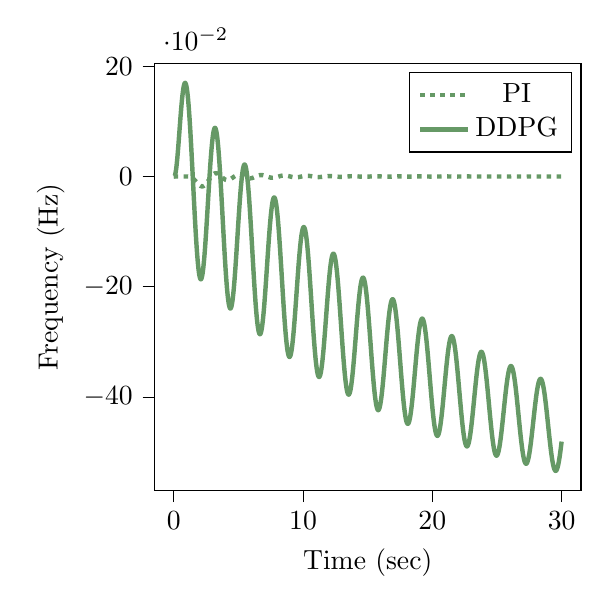
\begin{tikzpicture}

\definecolor{color0}{rgb}{0.12156862745098,0.466666666666667,0.705882352941177}
\definecolor{color1}{rgb}{1,0.498039215686275,0.0549019607843137}

\begin{axis}[
compat=newest,
tick align=outside,
tick pos=left,
x grid style={white!69.0196078431373!black},
xmin=-1.50000000000009, xmax=31.500000000002,
xtick style={color=black},
y grid style={white!69.0196078431373!black},
ymin=-0.569048370503337, ymax=0.204883272381782,
ytick style={color=black},
%yticklabel style={
%        /pgf/number format/.cd,
%        	fixed,
%        	fixed zerofill,
%         	precision=3,
%        /tikz/.cd
%},
scaled y ticks=true,
scaled y ticks=base 10:2,
width=7cm,
height=7cm,
xlabel=Time (sec),
ylabel=Frequency (Hz)
]
\addplot [ultra thick, green!20!gray, dotted]
table {%
0 0
0.01 0
0.02 0
0.03 0
0.04 0
0.05 0
0.06 0
0.07 0
0.08 0
0.09 0
0.1 0
0.11 0
0.12 0
0.13 0
0.14 0
0.15 0
0.16 0
0.17 0
0.18 0
0.19 0
0.2 0
0.21 0
0.22 0
0.23 0
0.24 0
0.25 0
0.26 0
0.27 0
0.28 0
0.29 0
0.3 0
0.31 0
0.32 0
0.33 0
0.34 0
0.35 0
0.36 0
0.37 0
0.38 0
0.39 0
0.4 0
0.41 0
0.42 0
0.43 0
0.44 0
0.45 0
0.46 0
0.47 0
0.48 0
0.49 0
0.5 0
0.51 0
0.52 0
0.53 0
0.54 0
0.55 0
0.56 0
0.57 0
0.58 0
0.59 0
0.6 0
0.61 0
0.62 0
0.63 0
0.64 0
0.65 0
0.66 0
0.67 0
0.68 0
0.69 0
0.7 0
0.71 0
0.72 0
0.73 0
0.74 0
0.75 0
0.76 0
0.77 0
0.78 0
0.79 0
0.8 0
0.81 0
0.820000000000001 0
0.830000000000001 0
0.840000000000001 0
0.850000000000001 0
0.860000000000001 0
0.870000000000001 0
0.880000000000001 0
0.890000000000001 0
0.900000000000001 0
0.910000000000001 0
0.920000000000001 0
0.930000000000001 0
0.940000000000001 0
0.950000000000001 0
0.960000000000001 0
0.970000000000001 0
0.980000000000001 0
0.990000000000001 0
1 0
1.01 -4.56702698575438e-08
1.02 -3.14412282210323e-07
1.03 -1.03224858863571e-06
1.04 -2.42692001312371e-06
1.05 -4.72220514793178e-06
1.06 -8.14114550207929e-06
1.07 -1.29054674852236e-05
1.08 -1.92351943429038e-05
1.09 -2.73483098595994e-05
1.1 -3.74604295610264e-05
1.11 -4.97844613317375e-05
1.12 -6.45302582465675e-05
1.13 -8.19042662493712e-05
1.14 -0.000102109168994071
1.15 -0.000125343531876731
1.16 -0.000151801447050597
1.17 -0.00018167218102023
1.18 -0.000215139826246024
1.19 -0.000252382958049325
1.2 -0.000293574297985703
1.21 -0.000338880384746122
1.22 -0.000388461253549982
1.23 -0.000442470124908258
1.24 -0.000501053103557714
1.25 -0.000564348888296994
1.26 -0.000632488493391376
1.27 -0.000705594982154219
1.28 -0.000783783213258725
1.29 -0.000867159600283394
1.3 -0.000955821884947396
1.31 -0.00104985892444807
1.32 -0.00114935049327104
1.33 -0.00125436709980434
1.34 -0.00136496981805016
1.35 -0.00148121013469254
1.36 -0.00160312981174468
1.37 -0.00173076076496695
1.38 -0.00186412495821491
1.39 -0.00200323431384583
1.4 -0.00214809063928263
1.41 -0.00229868556980549
1.42 -0.00245500052761286
1.43 -0.00261700669716682
1.44 -0.00278466501667225
1.45 -0.00295792618619637
1.46 -0.00313673069158975
1.47 -0.00332100884456962
1.48 -0.00351068083878698
1.49 -0.00370565682162715
1.5 -0.00390583698206329
1.51 -0.00411111165360954
1.52 -0.00432136143270295
1.53 -0.0045364573121556
1.54 -0.00475626082943241
1.55 -0.00498062422949103
1.56 -0.0052093906419006
1.57 -0.00544239427193859
1.58 -0.00567946060534774
1.59 -0.00592040662698311
1.6 -0.0061650410541343
1.61 -0.00641316457871866
1.62 -0.00666457012321627
1.63 -0.00691904310879842
1.64 -0.00717636173505131
1.65 -0.00743629727097169
1.66 -0.00769861439029244
1.67 -0.00796307140439868
1.68 -0.00822942060418756
1.69 -0.0084974086039717
1.7 -0.00876677667869147
1.71 -0.00903726110918077
1.72 -0.0093085935349716
1.73 -0.00958050131411414
1.74 -0.00985270788948236
1.75 -0.0101249331610275
1.76 -0.0103968938634371
1.77 -0.01066830394865
1.78 -0.0109388749727432
1.79 -0.0112083164864504
1.8 -0.0114763364288989
1.81 -0.0117426415239977
1.82 -0.0120069376788832
1.83 -0.0122689303838665
1.84 -0.0125283251133168
1.85 -0.0127848277269192
1.86 -0.0130381448707465
1.87 -0.013287984377585
1.88 -0.0135340556659596
1.89 -0.0137760701373067
1.9 -0.0140137415707465
1.91 -0.0142467865149136
1.92 -0.0144749246763098
1.93 -0.0146978793036483
1.94 -0.0149153775676687
1.95 -0.0151271509359078
1.96 -0.0153329355419192
1.97 -0.0155324725484477
1.98 -0.0157255085040693
1.99 -0.0159117956928221
2 -0.0160910924763613
2.01 -0.0162631636281865
2.02 -0.0164277806594973
2.03 -0.0165847221362496
2.04 -0.0167337739869955
2.05 -0.016874729801105
2.06 -0.0170073911170471
2.07 -0.0171315677126815
2.08 -0.0172470778421629
2.09 -0.0173537485094947
2.1 -0.0174514157133097
2.11 -0.0175399246799069
2.12 -0.0176191300842584
2.13 -0.0176888962587173
2.14 -0.017749097389171
2.15 -0.0177996176984012
2.16 -0.0178403516164308
2.17 -0.0178712039376503
2.18 -0.0178920899645405
2.19 -0.0179029356378194
2.2 -0.0179036776528659
2.21 -0.0178942635622843
2.22 -0.0178746518644997
2.23 -0.017844812078285
2.24 -0.0178047248031464
2.25 -0.0177543817655067
2.26 -0.0176937858506483
2.27 -0.017622951120394
2.28 -0.0175419028165252
2.29 -0.01745067734995
2.29999999999999 -0.017349322275659
2.30999999999999 -0.0172378962535171
2.31999999999999 -0.017116468994963
2.32999999999999 -0.0169851211956915
2.33999999999999 -0.0168439444544621
2.34999999999999 -0.0166930411780935
2.35999999999999 -0.0165325244728114
2.36999999999999 -0.0163625180234051
2.37999999999999 -0.0161831559564623
2.38999999999999 -0.0159945826902335
2.39999999999999 -0.0157969527743333
2.40999999999999 -0.0155904307152294
2.41999999999999 -0.0153751907890753
2.42999999999999 -0.0151514168420423
2.43999999999999 -0.014919302078276
2.44999999999999 -0.0146790488355468
2.45999999999999 -0.0144308684617544
2.46999999999999 -0.0141749815215782
2.47999999999999 -0.0139116163226356
2.48999999999999 -0.0136410093442461
2.49999999999999 -0.0133634049583651
2.50999999999999 -0.0130790551423308
2.51999999999999 -0.0127882191833656
2.52999999999999 -0.0124911633749482
2.53999999999999 -0.0121881607052759
2.54999999999999 -0.0118794905381046
2.55999999999999 -0.0115654382863014
2.56999999999999 -0.0112462950784786
2.57999999999999 -0.0109223574190995
2.58999999999999 -0.0105939268424684
2.59999999999999 -0.0102613095610289
2.60999999999999 -0.00992481610840887
2.61999999999999 -0.00958476097765819
2.62999999999999 -0.00924146225513431
2.63999999999999 -0.00889524125049722
2.64999999999999 -0.00854642212328069
2.65999999999999 -0.00819533150651048
2.66999999999999 -0.00784229812784497
2.67999999999999 -0.00748765242871479
2.68999999999999 -0.00713172618194104
2.69999999999999 -0.00677485210831213
2.70999999999999 -0.00641736349259943
2.71999999999999 -0.00605959379949268
2.72999999999999 -0.00570187628993329
2.73999999999999 -0.00534454363832393
2.74999999999999 -0.00498792755108879
2.75999999999999 -0.00463235838705714
2.76999999999998 -0.00427816478013842
2.77999999999998 -0.00392567326475337
2.78999999999998 -0.00357520790448088
2.79999999999998 -0.00322708992437457
2.80999999999998 -0.00288163734739737
2.81999999999998 -0.00253916463541585
2.82999999999998 -0.00219998233518921
2.83999999999998 -0.00186439672977979
2.84999999999998 -0.00153270949580389
2.85999999999998 -0.00120521736693388
2.86999999999998 -0.000882211804052241
2.87999999999998 -0.000563978672449437
2.88999999999998 -0.000250797926447132
2.89999999999998 5.7056698182097e-05
2.90999999999998 0.000359317983625507
2.91999999999998 0.000655725520916634
2.92999999999998 0.00094602599211228
2.93999999999998 0.00122997344314835
2.94999999999998 0.00150732954726987
2.95999999999998 0.00177786385868231
2.96999999999998 0.00204135405613818
2.97999999999998 0.00229758617618606
2.98999999999998 0.00254635483582348
2.99999999999998 0.00278746344430865
3.00999999999998 0.00302072440390081
3.01999999999998 0.00324595929931345
3.02999999999998 0.00346299907567922
3.03999999999998 0.00367168420484046
3.04999999999998 0.00387186483979472
3.05999999999998 0.00406340095713928
3.06999999999998 0.00424616248737467
3.07999999999998 0.0044200294329424
3.08999999999998 0.00458489197388755
3.09999999999998 0.00474065056103012
3.10999999999998 0.0048872159966561
3.11999999999998 0.00502450950257532
3.12999999999998 0.00515246277544806
3.13999999999998 0.00527101802947697
3.14999999999998 0.00538012802639291
3.15999999999998 0.00547975609273206
3.16999999999998 0.00556987612477479
3.17999999999998 0.00565047258172155
3.18999999999998 0.00572154046112989
3.19999999999998 0.00578308526778103
3.20999999999998 0.00583512296784114
3.21999999999998 0.00587767993055738
3.22999999999998 0.00591079285755505
3.23999999999997 0.00593450869979861
3.24999999999997 0.0059488845622667
3.25999999999997 0.00595398759636447
3.26999999999997 0.0059498948800471
3.27999999999997 0.00593669328554226
3.28999999999997 0.0059144793344106
3.29999999999997 0.00588335903942656
3.30999999999997 0.00584345030795974
3.31999999999997 0.00579487613380529
3.32999999999997 0.00573777019728154
3.33999999999997 0.0056722749888938
3.34999999999997 0.00559854160900058
3.35999999999997 0.00551672956104437
3.36999999999997 0.00542700654145486
3.37999999999997 0.00532954823298803
3.38999999999997 0.00522453814266034
3.39999999999997 0.00511216626202445
3.40999999999997 0.00499263031444395
3.41999999999997 0.00486613512761913
3.42999999999997 0.00473289219839315
3.43999999999997 0.00459311941524984
3.44999999999997 0.00444704077435877
3.45999999999997 0.00429488608952313
3.46999999999997 0.00413689069639515
3.47999999999997 0.00397329498435436
3.48999999999997 0.00380434407396633
3.49999999999997 0.00363028814409521
3.50999999999997 0.00345138162365781
3.51999999999997 0.00326788289322278
3.52999999999997 0.00308005397178049
3.53999999999997 0.0028881601958746
3.54999999999997 0.00269246989406197
3.55999999999997 0.00249325405818141
3.56999999999997 0.00229078601232922
3.57999999999997 0.00208534108018961
3.58999999999997 0.00187719258733167
3.59999999999997 0.00166662322865014
3.60999999999997 0.00145391221502489
3.61999999999997 0.00123933943681376
3.62999999999997 0.0010231851268333
3.63999999999997 0.000805729525174629
3.64999999999997 0.000587252546058484
3.65999999999997 0.000368033446989364
3.66999999999997 0.000148350500504407
3.67999999999997 -7.15193311649118e-05
3.68999999999997 -0.000291300718185713
3.69999999999997 -0.000510720281626398
3.70999999999996 -0.000729506908037226
3.71999999999996 -0.00094739205976098
3.72999999999996 -0.00116411008062261
3.73999999999996 -0.0013793984966628
3.74999999999996 -0.00159299831157998
3.75999999999996 -0.00180465429655127
3.76999999999996 -0.00201411527410899
3.77999999999996 -0.00222113439575707
3.78999999999996 -0.00242546941301932
3.79999999999996 -0.00262688294162014
3.80999999999996 -0.00282514271850724
3.81999999999996 -0.00302002185143558
3.82999999999996 -0.00321129906093341
3.83999999999996 -0.00339875891407068
3.84999999999996 -0.00358219205011439
3.85999999999996 -0.00376139539782446
3.86999999999996 -0.00393617238398743
3.87999999999996 -0.0041063331330459
3.88999999999996 -0.00427169465761873
3.89999999999996 -0.0044320810397194
3.90999999999996 -0.00458732360249194
3.91999999999996 -0.0047372610722959
3.92999999999996 -0.00488173973098484
3.93999999999996 -0.00502061355823467
3.94999999999996 -0.00515374436379172
3.95999999999996 -0.00528100190952229
3.96999999999996 -0.00540226402115892
3.97999999999996 -0.00551741668965081
3.98999999999996 -0.00562635416203904
3.99999999999996 -0.00572897902178935
4.00999999999996 -0.00582520225852801
4.01999999999996 -0.00591494332713832
4.02999999999996 -0.00599813019618698
4.03999999999996 -0.00607469938566092
4.04999999999996 -0.00614459599400559
4.05999999999996 -0.00620777371455361
4.06999999999996 -0.00626419484342007
4.07999999999996 -0.00631383026954371
4.08999999999996 -0.00635665946156727
4.09999999999996 -0.00639267050525298
4.10999999999996 -0.00642186025921436
4.11999999999996 -0.00644423377270094
4.12999999999996 -0.0064598045172029
4.13999999999996 -0.00646859432016435
4.14999999999996 -0.00647063328884705
4.15999999999996 -0.00646595972450315
4.16999999999996 -0.00645462002704155
4.17999999999996 -0.00643666859040992
4.18999999999996 -0.00641216768897437
4.19999999999995 -0.00638118735528696
4.20999999999995 -0.00634380524984481
4.21999999999995 -0.00630010652604824
4.22999999999995 -0.00625018368426875
4.23999999999995 -0.00619413643168278
4.24999999999995 -0.00613207155452776
4.25999999999995 -0.00606410190361618
4.26999999999995 -0.00599034744460079
4.27999999999995 -0.00591093479691688
4.28999999999995 -0.00582599683637805
4.29999999999995 -0.00573567250171466
4.30999999999995 -0.00564010659036509
4.31999999999995 -0.00553944954616248
4.32999999999995 -0.00543385724021395
4.33999999999995 -0.00532349074573674
4.34999999999995 -0.00520851610738762
4.35999999999995 -0.00508910410551723
4.36999999999995 -0.00496543001573138
4.37999999999995 -0.00483767336411753
4.38999999999995 -0.00470601767848254
4.39999999999995 -0.00457065023594328
4.40999999999995 -0.00443176180720864
4.41999999999995 -0.00428954639789181
4.42999999999995 -0.00414420098719166
4.43999999999995 -0.00399592526428246
4.44999999999995 -0.00384492136275236
4.45999999999995 -0.00369139359343035
4.46999999999995 -0.0035355453477114
4.47999999999995 -0.0033775876374996
4.48999999999995 -0.00321772965713743
4.49999999999995 -0.00305618170405383
4.50999999999995 -0.00289315490809815
4.51999999999995 -0.00272886096113903
4.52999999999995 -0.00256351184806272
4.53999999999995 -0.00239731957862205
4.54999999999995 -0.00223049592073848
4.55999999999995 -0.00206325213557735
4.56999999999995 -0.00189579871471302
4.57999999999995 -0.00172834511969806
4.58999999999995 -0.00156109952434565
4.59999999999995 -0.00139426856003046
4.60999999999995 -0.00122805706430858
4.61999999999995 -0.00106266783315121
4.62999999999995 -0.00089830137708213
4.63999999999995 -0.000735155681502113
4.64999999999995 -0.000573425971477527
4.65999999999995 -0.000413304481263418
4.66999999999994 -0.000254980228824893
4.67999999999994 -9.86387956123772e-05
4.68999999999994 5.55378881603969e-05
4.69999999999994 0.000207371752486784
4.70999999999994 0.000356688790570934
4.71999999999994 0.000503319255655039
4.72999999999994 0.000647097851396419
4.73999999999994 0.000787863915636973
4.74999999999994 0.000925461597355301
4.75999999999994 0.00105974002481702
4.76999999999994 0.00119055345817226
4.77999999999994 0.00131776147293568
4.78999999999994 0.00144122909161721
4.79999999999994 0.00156082692402237
4.80999999999994 0.00167643129975264
4.81999999999994 0.00178792439277951
4.82999999999994 0.00189519433797494
4.83999999999994 0.00199813533949171
4.84999999999994 0.00209664777096429
4.85999999999994 0.00219063826729141
4.86999999999994 0.00228001980781176
4.87999999999994 0.0023647117913946
4.88999999999994 0.00244463921318899
4.89999999999994 0.00251973564373065
4.90999999999994 0.00258994010222588
4.91999999999994 0.00265519824544995
4.92999999999994 0.0027154623996715
4.93999999999994 0.00277069158401271
4.94999999999994 0.00282085152525523
4.95999999999994 0.00286591466411331
4.96999999999994 0.00290586015519535
4.97999999999994 0.00294067385183946
4.98999999999994 0.00297034828918214
4.99999999999994 0.0029948826568622
5.00999999999994 0.00301428276335714
5.01999999999994 0.00302856099216281
5.02999999999994 0.00303773624991572
5.03999999999994 0.00304183390658215
5.04999999999994 0.00304088572785744
5.05999999999994 0.00303492979994373
5.06999999999994 0.00302401044691617
5.07999999999994 0.00300817814095308
5.08999999999994 0.00298748940680104
5.09999999999994 0.00296200671876972
5.10999999999994 0.00293179839098791
5.11999999999994 0.00289693846825622
5.12999999999994 0.00285750661730387
5.13999999999993 0.00281358803165423
5.14999999999993 0.0027652733840897
5.15999999999993 0.00271265763567614
5.16999999999993 0.0026558409978875
5.17999999999993 0.0025949288549291
5.18999999999993 0.00253003110384417
5.19999999999993 0.00246126205207508
5.20999999999993 0.0023887408913177
5.21999999999993 0.00231259091980459
5.22999999999993 0.00223293940690849
5.23999999999993 0.00214991742817973
5.24999999999993 0.00206365968637641
5.25999999999993 0.00197430432434541
5.26999999999993 0.00188199273232489
5.27999999999993 0.00178686935097737
5.28999999999993 0.00168908147092962
5.29999999999993 0.00158877902935227
5.30999999999993 0.0014861144039938
5.31999999999993 0.00138124220502378
5.32999999999993 0.0012743190650076
5.33999999999993 0.00116550342731696
5.34999999999993 0.00105495533327042
5.35999999999993 0.000942836208291411
5.36999999999993 0.000829308647367516
5.37999999999993 0.00071453620009114
5.38999999999993 0.000598683155559701
5.39999999999993 0.000481914327411189
5.40999999999993 0.000364394839268442
5.41999999999993 0.000246289910863508
5.42999999999993 0.000127764645110726
5.43999999999993 8.98381639447029e-06
5.44999999999993 -0.000109888339665201
5.45999999999993 -0.000228688334709431
5.46999999999993 -0.000347253634143528
5.47999999999993 -0.000465422861393727
5.48999999999993 -0.000583035999662597
5.49999999999993 -0.000699934590957058
5.50999999999993 -0.00081596193213827
5.51999999999993 -0.000930963267752629
5.52999999999993 -0.00104478597942291
5.53999999999993 -0.00115727977157408
5.54999999999993 -0.00126829685327541
5.55999999999993 -0.00137769211598698
5.56999999999993 -0.00148532330700467
5.57999999999993 -0.00159105119840394
5.58999999999993 -0.00169473975128986
5.59999999999993 -0.00179625627516714
5.60999999999992 -0.00189547158225157
5.61999999999992 -0.00199226013655087
5.62999999999992 -0.0020865001975511
5.63999999999992 -0.00217807395835176
5.64999999999992 -0.00226686767810109
5.65999999999992 -0.00235277180859027
5.66999999999992 -0.00243568111487424
5.67999999999992 -0.0025154947897942
5.68999999999992 -0.00259211656228566
5.69999999999992 -0.00266545479936417
5.70999999999992 -0.00273542260168956
5.71999999999992 -0.00280193789261796
5.72999999999992 -0.00286492350065963
5.73999999999992 -0.00292430723526952
5.74999999999992 -0.0029800219559062
5.75999999999992 -0.00303200563430371
5.76999999999992 -0.00308020140990979
5.77999999999992 -0.00312455763845315
5.78999999999992 -0.00316502793361096
5.79999999999992 -0.00320157120175746
5.80999999999992 -0.00323415166978314
5.81999999999992 -0.00326273890769518
5.82999999999992 -0.00328730783989478
5.83999999999992 -0.00330783875224398
5.84999999999992 -0.00332431729318785
5.85999999999992 -0.0033367344671051
5.86999999999992 -0.00334508662086859
5.87999999999992 -0.00334937542367718
5.88999999999992 -0.00334960784023563
5.89999999999992 -0.00334579609737833
5.90999999999992 -0.00333795764425978
5.91999999999992 -0.00332611510627616
5.92999999999992 -0.00331029623295033
5.93999999999992 -0.00329053384013617
5.94999999999992 -0.00326686574713574
5.95999999999992 -0.00323933470981761
5.96999999999992 -0.00320798835193645
5.97999999999992 -0.00317287909960448
5.98999999999992 -0.00313406413139951
5.99999999999992 -0.00309160537036543
6.00999999999992 -0.00304556928628709
6.01999999999992 -0.00299602508243559
6.02999999999992 -0.00294304742333545
6.03999999999992 -0.00288671512814451
6.04999999999992 -0.0028271110495327
6.05999999999992 -0.0027643219480957
6.06999999999992 -0.00269843836225924
6.07999999999991 -0.0026295542340756
6.08999999999991 -0.00255776690913475
6.09999999999991 -0.00248317767256908
6.10999999999991 -0.00240589092875839
6.11999999999991 -0.00232601410087476
6.12999999999991 -0.00224365750158161
6.13999999999991 -0.00215893418978857
6.14999999999991 -0.00207195981944098
6.15999999999991 -0.00198285248307801
6.16999999999991 -0.00189173255157262
6.17999999999991 -0.0017987225108806
6.18999999999991 -0.00170394679634644
6.19999999999991 -0.00160753162190045
6.20999999999991 -0.00150960481450305
6.21999999999991 -0.00141029564562073
6.22999999999991 -0.0013097346559048
6.23999999999991 -0.00120805348233963
6.24999999999991 -0.00110538468471566
6.25999999999991 -0.00100186157166898
6.26999999999991 -0.000897618026522447
6.27999999999991 -0.000792788333159092
6.28999999999991 -0.000687507002154885
6.29999999999991 -0.000581908597394639
6.30999999999991 -0.000476127563392593
6.31999999999991 -0.000370298053535927
6.32999999999991 -0.000264553759467204
6.33999999999991 -0.000159027741818617
6.34999999999991 -5.3852262508059e-05
6.35999999999991 5.08413811959412e-05
6.36999999999991 0.000154923020637339
6.37999999999991 0.000258263777554773
6.38999999999991 0.000360736223514815
6.39999999999991 0.000462214536773481
6.40999999999991 0.000562574656387694
6.41999999999991 0.000661694433395888
6.42999999999991 0.000759458871543323
6.43999999999991 0.000855745217284463
6.44999999999991 0.000950437929328321
6.45999999999991 0.00104342394551219
6.46999999999991 0.00113459281706554
6.47999999999991 0.00122383683890799
6.48999999999991 0.001311051175838
6.49999999999991 0.00139613398447413
6.50999999999991 0.00147898653081626
6.51999999999991 0.00155951330329951
6.52999999999991 0.00163762212121979
6.53999999999991 0.00171322423841503
6.5499999999999 0.00178623444209335
6.5599999999999 0.00185657114670457
6.5699999999999 0.00192414952078153
6.5799999999999 0.00198890259266039
6.5899999999999 0.00205076021142161
6.5999999999999 0.0021096561809031
6.6099999999999 0.00216552832729217
6.6199999999999 0.00221831856131671
6.6299999999999 0.00226797293497879
6.6399999999999 0.00231444169278139
6.6499999999999 0.00235767931740654
6.6599999999999 0.00239764456981063
6.6699999999999 0.00243430052371025
6.6799999999999 0.0024676145944395
6.6899999999999 0.00249755856216717
6.6999999999999 0.0025241085894701
6.7099999999999 0.0025472452348407
6.7199999999999 0.00256695345657212
6.7299999999999 0.00258322261333067
6.7399999999999 0.00259604646021315
6.7499999999999 0.00260542313832703
6.7599999999999 0.00261135515887606
6.7699999999999 0.0026138493818104
6.7799999999999 0.00261291698911464
6.7899999999999 0.0026085734528259
6.7999999999999 0.00260083849790064
6.8099999999999 0.00258973606008942
6.8199999999999 0.00257529423904414
6.8299999999999 0.00255754524700381
6.8399999999999 0.00253652535361347
6.8499999999999 0.00251227482786934
6.8599999999999 0.00248483787910447
6.8699999999999 0.00245426260105603
6.8799999999999 0.00242060092452187
6.8899999999999 0.00238390849986336
6.8999999999999 0.00234424464827162
6.9099999999999 0.00230167141454017
6.9199999999999 0.00225625430184514
6.9299999999999 0.00220806258182843
6.9399999999999 0.00215716874840198
6.9499999999999 0.00210364841166128
6.9599999999999 0.00204758018841835
6.9699999999999 0.00198904511263188
6.9799999999999 0.00192812735112422
6.9899999999999 0.00186491400935433
6.9999999999999 0.00179949472907191
7.00999999999989 0.00173196150846321
7.01999999999989 0.00166240859926983
7.02999999999989 0.00159093239077703
7.03999999999989 0.00151763128595354
7.04999999999989 0.00144260557265333
7.05999999999989 0.00136595729137589
7.06999999999989 0.00128779010044417
7.07999999999989 0.00120820913915048
7.08999999999989 0.00112732088926347
7.09999999999989 0.00104523303520358
7.10999999999989 0.000962054323147272
7.11999999999989 0.000877894419291845
7.12999999999989 0.000792863767496115
7.13999999999989 0.000707073446501297
7.14999999999989 0.000620635026929133
7.15999999999989 0.000533660428249744
7.16999999999989 0.000446261775907354
7.17999999999989 0.000358551258789548
7.18999999999989 0.000270640987222589
7.19999999999989 0.000182642851673209
7.20999999999989 9.46683823346566e-05
7.21999999999989 6.82860976681752e-06
7.22999999999989 -8.07660732364912e-05
7.23999999999989 -0.00016800604834793
7.24999999999989 -0.000254782606853351
7.25999999999989 -0.000340988083063305
7.26999999999989 -0.000426515985819924
7.27999999999989 -0.000511265435743074
7.28999999999989 -0.000595128695006298
7.29999999999989 -0.000678003564573575
7.30999999999989 -0.000759789519002424
7.31999999999989 -0.00084038782648568
7.32999999999989 -0.000919701666064654
7.33999999999989 -0.000997636241882978
7.34999999999989 -0.00107409889435306
7.35999999999989 -0.00114899920811171
7.36999999999989 -0.00122224911664505
7.37999999999989 -0.00129376300322991
7.38999999999989 -0.001363457798627
7.39999999999989 -0.00143125307553262
7.40999999999989 -0.00149707113844429
7.41999999999989 -0.00156083710998829
7.42999999999989 -0.00162247901329206
7.43999999999989 -0.00168192785031396
7.44999999999989 -0.00173911767604824
7.45999999999989 -0.00179397841225827
7.46999999999989 -0.0018464578248494
7.47999999999988 -0.00189649958341368
7.48999999999988 -0.00194405066786694
7.49999999999988 -0.00198906142093598
7.50999999999988 -0.00203148559617937
7.51999999999988 -0.00207128040149992
7.52999999999988 -0.00210840653811307
7.53999999999988 -0.00214282823494169
7.54999999999988 -0.00217451327841414
7.55999999999988 -0.00220343303791404
7.56999999999988 -0.00222956248575201
7.57999999999988 -0.00225288021325329
7.58999999999988 -0.00227336844400992
7.59999999999988 -0.00229101303727037
7.60999999999988 -0.00230580349103359
7.61999999999988 -0.00231773294002165
7.62999999999988 -0.00232679814864851
7.63999999999988 -0.00233299949949029
7.64999999999988 -0.00233634097731353
7.65999999999988 -0.0023368301487349
7.66999999999988 -0.00233447813760962
7.67999999999988 -0.00232929959628168
7.68999999999988 -0.00232131267288649
7.69999999999988 -0.0023105389749946
7.70999999999988 -0.00229700353006224
7.71999999999988 -0.00228073474349196
7.72999999999988 -0.00226176435580089
7.73999999999988 -0.00224012738790183
7.74999999999988 -0.00221586206834461
7.75999999999988 -0.0021890097955682
7.76999999999988 -0.0021596150959424
7.77999999999988 -0.00212772559382635
7.78999999999988 -0.0020933906602953
7.79999999999988 -0.00205666341062924
7.80999999999988 -0.00201759974120621
7.81999999999988 -0.00197625824612597
7.82999999999988 -0.00193270013092413
7.83999999999988 -0.00188698912347598
7.84999999999988 -0.00183919138219689
7.85999999999988 -0.00178937482251545
7.86999999999988 -0.0017376102932181
7.87999999999988 -0.00168397075529473
7.88999999999988 -0.00162853118715017
7.89999999999988 -0.00157136851820769
7.90999999999988 -0.00151256149706831
7.91999999999988 -0.00145219057401148
7.92999999999988 -0.00139033779914695
7.93999999999988 -0.00132708671625768
7.94999999999987 -0.00126252225367742
7.95999999999987 -0.00119673061298357
7.96999999999987 -0.00112979915600753
7.97999999999987 -0.00106181629051712
7.98999999999987 -0.000992871354845572
7.99999999999987 -0.000923054501695055
8.00999999999987 -0.00085245658131511
8.01999999999987 -0.000781169024239489
8.02999999999987 -0.000709283723753719
8.03999999999987 -0.000636892918258511
8.04999999999987 -0.000564089073688896
8.05999999999987 -0.000490964766145133
8.06999999999987 -0.000417612564888299
8.07999999999987 -0.000344124915850528
8.08999999999987 -0.000270594025808506
8.09999999999987 -0.000197111747364978
8.10999999999987 -0.000123769464882233
8.11999999999987 -5.06579815086466e-05
8.12999999999987 2.21325925631992e-05
8.13999999999987 9.45163776568688e-05
8.14999999999987 0.000166401961630369
8.15999999999987 0.000237701975107046
8.16999999999987 0.000308330168557878
8.17999999999987 0.00037820151621999
8.18999999999987 0.00044723231796884
8.19999999999987 0.000515340299030038
8.20999999999987 0.000582444707419217
8.21999999999987 0.000648466409001026
8.22999999999987 0.00071332798006082
8.23999999999987 0.000776953797286301
8.24999999999987 0.000839270125058816
8.25999999999987 0.000900205199957883
8.26999999999987 0.000959689312386331
8.27999999999987 0.00101765488516002
8.28999999999987 0.00107403654876454
8.29999999999987 0.0011287712146525
8.30999999999987 0.00118179814407977
8.31999999999987 0.00123305901407116
8.32999999999987 0.00128249798002975
8.33999999999987 0.00133006173492477
8.34999999999987 0.00137569956499714
8.35999999999987 0.0014193634019255
8.36999999999987 0.00146100787139982
8.37999999999987 0.0015005829145111
8.38999999999987 0.00153805635480369
8.39999999999987 0.00157339122130214
8.40999999999987 0.00160655339730183
8.41999999999986 0.00163751165047405
8.42999999999986 0.00166623765920532
8.43999999999986 0.00169270603515565
8.44999999999986 0.00171689434202522
8.45999999999986 0.00173878311052507
8.46999999999986 0.00175835585036807
8.47999999999986 0.00177559905704414
8.48999999999986 0.00179050221402876
8.49999999999986 0.00180305779381102
8.50999999999986 0.00181326125402478
8.51999999999986 0.00182111102988873
8.52999999999986 0.00182660852300417
8.53999999999986 0.0018297580865748
8.54999999999986 0.0018305670071348
8.55999999999986 0.00182904548290507
8.56999999999986 0.00182520659895015
8.57999999999986 0.00181906629939776
8.58999999999986 0.0018106433571411
8.59999999999986 0.00179995933620257
8.60999999999986 0.00178703854696338
8.61999999999986 0.00177190800993024
8.62999999999986 0.00175459741406812
8.63999999999986 0.00173513907513339
8.64999999999986 0.00171356789760961
8.65999999999986 0.00168992135042917
8.66999999999986 0.00166423886367784
8.67999999999986 0.00163656214111643
8.68999999999986 0.00160693556871751
8.69999999999986 0.00157540578416521
8.70999999999986 0.00154202160724568
8.71999999999986 0.00150683396790039
8.72999999999986 0.00146989583202592
8.73999999999986 0.00143126212511028
8.74999999999986 0.00139098921541599
8.75999999999986 0.00134913577000233
8.76999999999986 0.00130576218457999
8.77999999999986 0.00126093047188826
8.78999999999986 0.00121470418229002
8.79999999999986 0.0011671483201374
8.80999999999986 0.00111832925731685
8.81999999999986 0.00106831465084782
8.82999999999986 0.00101717335476452
8.83999999999986 0.000964975315842185
8.84999999999986 0.00091179148111756
8.85999999999986 0.000857693705452511
8.86999999999986 0.000802754657904446
8.87999999999986 0.000747047727185088
8.88999999999985 0.000690646926430347
8.89999999999985 0.000633626797468552
8.90999999999985 0.000576062314752243
8.91999999999985 0.000518028789105362
8.92999999999985 0.000459601771427792
8.93999999999985 0.000400856956493254
8.94999999999985 0.000341870086971406
8.95999999999985 0.000282716857801801
8.96999999999985 0.000223472821044256
8.97999999999985 0.000164213291327513
8.98999999999985 0.000105013252016191
8.99999999999985 4.59472622131754e-05
9.00999999999985 -1.29106352866928e-05
9.01999999999985 -7.14870049779854e-05
9.02999999999985 -0.000129712272538907
9.03999999999985 -0.000187511753973662
9.04999999999985 -0.000244814371600656
9.05999999999985 -0.000301550001308893
9.06999999999985 -0.000357649556900692
9.07999999999985 -0.00041304507270506
9.08999999999985 -0.000467669784370108
9.09999999999985 -0.00052145820774507
9.10999999999985 -0.000574346215764377
9.11999999999985 -0.00062627111324861
9.12999999999985 -0.000677171709539574
9.13999999999985 -0.000726988388889401
9.14999999999985 -0.000775663178526504
9.15999999999985 -0.00082313981432399
9.16999999999985 -0.000869363803667021
9.17999999999985 -0.000914282486639798
9.18999999999985 -0.000957845093984301
9.19999999999985 -0.00100000280240599
9.20999999999985 -0.00104070878724629
9.21999999999985 -0.0010799182723771
9.22999999999985 -0.00111758857726544
9.23999999999985 -0.0011536791611595
9.24999999999985 -0.00118815166435088
9.25999999999985 -0.00122096284540454
9.26999999999985 -0.00125208612054794
9.27999999999985 -0.00128148995874762
9.28999999999985 -0.00130914514745527
9.29999999999985 -0.00133502481885508
9.30999999999985 -0.00135910447303366
9.31999999999985 -0.00138136199805862
9.32999999999985 -0.0014017776869567
9.33999999999985 -0.00142033425158686
9.34999999999985 -0.00143701683354432
9.35999999999984 -0.00145181301293943
9.36999999999984 -0.00146471281020877
9.37999999999984 -0.00147570868911612
9.38999999999984 -0.00148479555520942
9.39999999999984 -0.00149197075125953
9.40999999999984 -0.00149723404972304
9.41999999999984 -0.00150058764228631
9.42999999999984 -0.00150203612656783
9.43999999999984 -0.00150158649005259
9.44999999999984 -0.00149924808922244
9.45999999999984 -0.00149503262634541
9.46999999999984 -0.00148895412490803
9.47999999999984 -0.00148102890212317
9.48999999999984 -0.00147127553906187
9.49999999999984 -0.00145971484870804
9.50999999999984 -0.00144636984244506
9.51999999999984 -0.00143126569593979
9.52999999999984 -0.00141442971645245
9.53999999999984 -0.00139589131675814
9.54999999999984 -0.00137568188548628
9.55999999999984 -0.00135383413193229
9.56999999999984 -0.00133038322291184
9.57999999999984 -0.00130536619298665
9.58999999999984 -0.00127882188854218
9.59999999999984 -0.00125079090992076
9.60999999999984 -0.00122131555167681
9.61999999999984 -0.00119043974102567
9.62999999999984 -0.00115820871996682
9.63999999999984 -0.0011246694078592
9.64999999999984 -0.00108987030787925
9.65999999999984 -0.00105386127617251
9.66999999999984 -0.0010166934588677
9.67999999999984 -0.00097841922495073
9.68999999999984 -0.000939092096496868
9.69999999999984 -0.00089876667700411
9.70999999999984 -0.000857498578249446
9.71999999999984 -0.000815344345940021
9.72999999999984 -0.000772361384356347
9.73999999999984 -0.000728607880344804
9.74999999999984 -0.000684142730719668
9.75999999999984 -0.000639025460472026
9.76999999999984 -0.000593316142760465
9.77999999999984 -0.000547075320981842
9.78999999999984 -0.000500363930479687
9.79999999999984 -0.000453243220024529
9.80999999999984 -0.000405774673190206
9.81999999999984 -0.000358019929742412
9.82999999999983 -0.000310040707150967
9.83999999999983 -0.000261898722333029
9.84999999999983 -0.000213655613731913
9.85999999999983 -0.000165372863833075
9.86999999999983 -0.000117111722013049
9.87999999999983 -6.89331283653665e-05
9.88999999999983 -2.08976385447133e-05
9.89999999999983 2.69346513641876e-05
9.90999999999983 7.45041786834786e-05
9.91999999999983 0.000121751986976972
9.92999999999983 0.000168623077870492
9.93999999999983 0.000215057073634406
9.94999999999983 0.000260997256692289
9.95999999999983 0.000306387791058368
9.96999999999983 0.000351173789091529
9.97999999999983 0.000395301376719666
9.98999999999983 0.000438717757062323
9.99999999999983 0.000481371272381266
10.0099999999998 0.000523211464290874
10.0199999999998 0.000564189132161459
10.0299999999998 0.000604256389651809
10.0399999999998 0.000643366719308715
10.0499999999998 0.000681475025041648
10.0599999999998 0.000718537682710876
10.0699999999998 0.000754512588878808
10.0799999999998 0.000789359206913711
10.0899999999998 0.000823038611081555
10.0999999999998 0.000855513528385812
10.1099999999998 0.000886748378111065
10.1199999999998 0.00091670255985169
10.1299999999998 0.000945350800653097
10.1399999999998 0.000972662872950677
10.1499999999998 0.000998610377853765
10.1599999999998 0.0010231667727536
10.1699999999998 0.00104630739645606
10.1799999999998 0.0010680094918202
10.1899999999998 0.00108825222588731
10.1999999999998 0.00110701670748855
10.2099999999998 0.00112428600232277
10.2199999999998 0.00114004514550015
10.2299999999998 0.00115428115155105
10.2399999999998 0.00116698302272623
10.2499999999998 0.00117814175261023
10.2599999999998 0.00118775032866808
10.2699999999998 0.00119580373260837
10.2799999999998 0.00120229893784951
10.2899999999998 0.00120723490388575
10.2999999999998 0.00121061256838372
10.3099999999998 0.00121243483711803
10.3199999999998 0.00121270657150578
10.3299999999998 0.00121143457378336
10.3399999999998 0.00120862756988004
10.3499999999998 0.00120429619005826
10.3599999999998 0.00119845294741539
10.3699999999998 0.00119111221438164
10.3799999999998 0.0011822901974225
10.3899999999998 0.00117200491028896
10.3999999999998 0.0011602761464453
10.4099999999998 0.00114712545194677
10.4199999999998 0.0011325761016784
10.4299999999998 0.001116653087591
10.4399999999998 0.00109938250628217
10.4499999999998 0.00108079228458852
10.4599999999998 0.00106091200538854
10.4699999999998 0.00103977275102846
10.4799999999998 0.00101740705677433
10.4899999999998 0.000993848862702358
10.4999999999998 0.000969133464084768
10.5099999999998 0.000943297460331971
10.5199999999998 0.000916378385439326
10.5299999999998 0.000888415351245459
10.5399999999998 0.000859448596510812
10.5499999999998 0.000829519435177971
10.5599999999998 0.000798670203267155
10.5699999999998 0.000766944202976052
10.5799999999998 0.000734385644905735
10.5899999999998 0.000701039588895752
10.5999999999998 0.000666951883756984
10.6099999999998 0.000632169106097437
10.6199999999998 0.000596738498388166
10.6299999999998 0.00056070790639091
10.6399999999998 0.000524125716054054
10.6499999999998 0.000487040789975337
10.6599999999998 0.000449502403232602
10.6699999999998 0.000411560179603056
10.6799999999998 0.000373264027534041
10.6899999999998 0.000334664075440996
10.6999999999998 0.00029581060743574
10.7099999999998 0.000256754000125449
10.7199999999998 0.000217544657272024
10.7299999999998 0.000178232945553915
10.7399999999998 0.000138869131146439
10.7499999999998 9.95033166967193e-05
10.7599999999998 6.01853787757444e-05
10.7699999999998 2.09649058873616e-05
10.7799999999998 -1.81088628871264e-05
10.7899999999998 -5.69870985319079e-05
10.7999999999998 -9.56214419523214e-05
10.8099999999998 -0.000133964062971636
10.8199999999998 -0.000171967718393726
10.8299999999998 -0.000209585809063855
10.8399999999998 -0.00024677607236811
10.8499999999998 -0.000283490120027084
10.8599999999998 -0.000319683601245528
10.8699999999998 -0.000355313022698709
10.8799999999998 -0.000390335799766559
10.8899999999998 -0.000424710306368844
10.8999999999998 -0.000458395923346253
10.9099999999998 -0.000491353085334423
10.9199999999998 -0.000523543326079269
10.9299999999998 -0.000554929322099044
10.9399999999998 -0.000585474934581354
10.9499999999998 -0.000615145250145122
10.9599999999998 -0.000643906619234987
10.9699999999998 -0.000671720654112875
10.9799999999998 -0.000698562306054374
10.9899999999998 -0.000724401983760126
10.9999999999998 -0.000749211497757891
11.0099999999998 -0.000772964089744391
11.0199999999998 -0.000795634459979633
11.0299999999998 -0.000817198792709197
11.0399999999998 -0.000837634779592808
11.0499999999998 -0.000856921641119825
11.0599999999998 -0.000875040145995421
11.0699999999998 -0.000891972628483832
11.0799999999998 -0.000907703003892881
11.0899999999998 -0.00092221678176409
11.0999999999998 -0.000935501076675129
11.1099999999998 -0.00094754461727536
11.1199999999998 -0.000958337753480105
11.1299999999998 -0.000967872461527353
11.1399999999998 -0.00097614234562745
11.1499999999998 -0.000983142639429546
11.1599999999998 -0.000988870204708516
11.1699999999998 -0.000993323528011727
11.1799999999998 -0.000996502715283516
11.1899999999998 -0.000998409484489393
11.1999999999998 -0.000999047156266731
11.2099999999998 -0.000998420642634794
11.2199999999998 -0.000996536433804875
11.2299999999998 -0.00099340258310352
11.2399999999998 -0.000989028689966679
11.2499999999998 -0.00098342588173966
11.2599999999998 -0.000976606793504984
11.2699999999998 -0.000968585546705244
11.2799999999998 -0.000959377726845096
11.2899999999998 -0.000949000361043
11.2999999999998 -0.000937471897100896
11.3099999999998 -0.00092481218842962
11.3199999999998 -0.000911042260379857
11.3299999999998 -0.00089618423633222
11.3399999999998 -0.000880261784919938
11.3499999999998 -0.00086329981588172
11.3599999999998 -0.000845324442589411
11.3699999999998 -0.000826362943278396
11.3799999999998 -0.000806443721026517
11.3899999999998 -0.000785596262530244
11.3999999999998 -0.0007638509474297
11.4099999999998 -0.00074123921663512
11.4199999999998 -0.000717793594404038
11.4299999999998 -0.000693547500549578
11.4399999999998 -0.000668535208645431
11.4499999999998 -0.000642791801300231
11.4599999999998 -0.000616353123592802
11.4699999999998 -0.00058925573520641
11.4799999999998 -0.000561536861552821
11.4899999999998 -0.000533234344092381
11.4999999999998 -0.00050438658997747
11.5099999999998 -0.000475032521130089
11.5199999999998 -0.00044521152284641
11.5299999999998 -0.000414963392011692
11.5399999999998 -0.000384328285003565
11.5499999999998 -0.00035334666535805
11.5599999999998 -0.0003220592512707
11.5699999999998 -0.000290506963003237
11.5799999999998 -0.000258730870265259
11.5899999999998 -0.000226772139639505
11.5999999999998 -0.000194671982118118
11.6099999999998 -0.000162471600817
11.6199999999998 -0.000130212138934117
11.6299999999998 -9.79346280171962e-05
11.6399999999998 -6.56799366052351e-05
11.6499999999998 -3.348871930742e-05
11.6599999999998 -1.40136638221108e-06
11.6699999999998 3.05420461217303e-05
11.6799999999998 6.23018056013361e-05
11.6899999999998 9.38386114545741e-05
11.6999999999998 0.000125113622894027
11.7099999999998 0.00015608850596292
11.7199999999998 0.000186725479697476
11.7299999999998 0.000216987361381003
11.7399999999998 0.000246837610836535
11.7499999999998 0.000276240373706411
11.7599999999998 0.000305160523668528
11.7699999999998 0.000333563703540704
11.7799999999998 0.000361416365226251
11.7899999999998 0.000388685808455418
11.7999999999998 0.000415340218279229
11.8099999999998 0.000441348701273977
11.8199999999998 0.00046668132040069
11.8299999999998 0.000491309128545068
11.8399999999998 0.000515204200607852
11.8499999999998 0.000538339664168755
11.8599999999998 0.000560689728683201
11.8699999999998 0.000582229713178955
11.8799999999998 0.00060293607242446
11.8899999999998 0.000622786421542853
11.8999999999998 0.000641759559047619
11.9099999999998 0.00065983548827808
11.9199999999998 0.000676995437214944
11.9299999999998 0.000693221876658407
11.9399999999998 0.00070849853675339
11.9499999999998 0.000722810421848765
11.9599999999998 0.000736143823679587
11.9699999999998 0.000748486332863608
11.9799999999998 0.000759826848705588
11.9899999999998 0.000770155587305133
11.9999999999998 0.000779464087966187
12.0099999999998 0.000787745218459989
12.0199999999998 0.000794993177015
12.0299999999998 0.000801203493973973
12.0399999999998 0.000806373031573689
12.0499999999998 0.000810499981918136
12.0599999999998 0.000813583863292891
12.0699999999998 0.000815625514837007
12.0799999999998 0.000816627089592465
12.0899999999998 0.000816592045955631
12.0999999999998 0.000815525137560909
12.1099999999998 0.000813432401634672
12.1199999999998 0.00081032114586907
12.1299999999998 0.000806199933883561
12.1399999999998 0.000801078569372492
12.1499999999998 0.000794968079092888
12.1599999999998 0.000787880694870428
12.1699999999998 0.000779829834262052
12.1799999999998 0.00077083008415309
12.1899999999998 0.000760897184964323
12.1999999999998 0.000750048024754471
12.2099999999998 0.000738300126486093
12.2199999999998 0.000725672386080596
12.2299999999998 0.000712184739546754
12.2399999999998 0.000697858120465698
12.2499999999998 0.000682714428759921
12.2599999999998 0.000666776498421705
12.2699999999998 0.000650068064240012
12.2799999999998 0.000632613712491771
12.2899999999998 0.000614438676816775
12.2999999999998 0.000595569229509482
12.3099999999998 0.000576032388523409
12.3199999999998 0.000555855885017776
12.3299999999998 0.000535068127753012
12.3399999999998 0.000513698165645348
12.3499999999998 0.000491775649083596
12.3599999999998 0.000469330790326007
12.3699999999998 0.000446394323168457
12.3799999999998 0.000422997462013633
12.3899999999998 0.000399171860439475
12.3999999999998 0.000374949569348031
12.4099999999998 0.000350362994765995
12.4199999999998 0.000325444855362654
12.4299999999998 0.000300228139747347
12.4399999999998 0.000274746063606199
12.4499999999998 0.000249032026736475
12.4599999999998 0.000223119570035758
12.4699999999998 0.000197042332502164
12.4799999999998 0.000170834008301292
12.4899999999998 0.000144528303954771
12.4999999999998 0.000118158895704687
12.5099999999998 9.17593871075887e-05
12.5199999999998 6.53632669110663e-05
12.5299999999998 3.90038672651812e-05
12.5399999999998 1.27143223203448e-05
12.5499999999998 -1.34724727375367e-05
12.5599999999998 -3.95239021644559e-05
12.5699999999998 -6.54076695997141e-05
12.5799999999998 -9.10918374229726e-05
12.5899999999998 -0.000116544865479221
12.5999999999998 -0.000141735649125977
12.6099999999998 -0.000166633556557545
12.6199999999998 -0.000191208465362316
12.6299999999998 -0.000215430798270437
12.6399999999998 -0.000239271558050149
12.6499999999998 -0.000262702361512677
12.6599999999998 -0.000285695472586933
12.6699999999998 -0.000308223834425647
12.6799999999998 -0.00033026110050673
12.6899999999998 -0.000351781664696648
12.6999999999998 -0.000372760690236389
12.7099999999998 -0.000393174137630943
12.7199999999998 -0.000412998791411805
12.7299999999998 -0.000432212285717449
12.7399999999998 -0.000450793128692548
12.7499999999998 -0.000468720725671753
12.7599999999998 -0.000485975401124327
12.7699999999998 -0.000502538419337567
12.7799999999998 -0.000518392003818632
12.7899999999998 -0.000533519355396173
12.7999999999998 -0.000547904669004873
12.8099999999998 -0.000561533149137797
12.8199999999998 -0.000574391023953152
12.8299999999998 -0.000586465558023957
12.8399999999998 -0.000597745063720844
12.8499999999998 -0.000608218911220027
12.8599999999998 -0.000617877537130377
12.8699999999998 -0.000626712451735285
12.8799999999998 -0.000634716244846936
12.8899999999998 -0.000641882590456069
12.8999999999998 -0.000648206249735277
12.9099999999998 -0.000653683072290751
12.9199999999998 -0.000658309996810792
12.9299999999998 -0.000662085050014318
12.9399999999998 -0.000665007344238559
12.9499999999998 -0.000667077073678104
12.9599999999998 -0.000668295509290251
12.9699999999998 -0.000668664992384906
12.9799999999998 -0.000668188926921394
12.9899999999998 -0.000666871770540051
12.9999999999998 -0.000664719024364269
13.0099999999998 -0.000661737221620589
13.0199999999998 -0.000657933915143796
13.0299999999998 -0.000653317663867968
13.0399999999998 -0.00064789801846748
13.0499999999998 -0.000641685506439323
13.0599999999998 -0.000634691617198835
13.0699999999998 -0.00062692878844871
13.0799999999998 -0.000618410397161727
13.0899999999998 -0.000609150547372807
13.0999999999998 -0.000599164155265655
13.1099999999998 -0.000588467135408715
13.1199999999998 -0.000577076228955665
13.1299999999998 -0.000565008978514589
13.1399999999998 -0.000552283702152224
13.1499999999998 -0.000538919466564531
13.1599999999998 -0.000524936059446805
13.1699999999998 -0.000510353857985212
13.1799999999998 -0.00049519395333336
13.1899999999998 -0.00047947815310164
13.1999999999998 -0.000463228860010652
13.2099999999998 -0.00044646904385846
13.2199999999998 -0.000429222211560478
13.2299999999998 -0.000411512375975141
13.2399999999998 -0.000393364023867637
13.2499999999998 -0.000374802083210319
13.2599999999998 -0.000355851889946886
13.2699999999998 -0.00033653915431163
13.2799999999998 -0.000316889926776154
13.2899999999998 -0.000296930563685383
13.2999999999998 -0.000276687692638663
13.3099999999998 -0.000256188177668025
13.3199999999998 -0.000235459084263311
13.3299999999998 -0.000214527644292453
13.3399999999998 -0.000193421220863999
13.3499999999998 -0.000172167273178294
13.3599999999998 -0.000150793321412969
13.3699999999998 -0.000129326911687925
13.3799999999998 -0.000107795581154347
13.3899999999998 -8.62268232519189e-05
13.3999999999998 -6.46480531777433e-05
13.4099999999998 -4.30865736099457e-05
13.4199999999998 -2.15695407284658e-05
13.4299999999998 -1.23930574753726e-07
13.4399999999998 2.12234942084823e-05
13.4499999999998 4.24462172166787e-05
13.4599999999998 6.35180006633231e-05
13.4699999999998 8.44129172601673e-05
13.4799999999998 0.000105105381560324
13.4899999999998 0.000125570180726871
13.4999999999998 0.000145782504690656
13.5099999999998 0.00016571797566191
13.5199999999998 0.000185352676961279
13.5299999999998 0.000204663181136887
13.5399999999998 0.000223626577335153
13.5499999999998 0.000242220497894078
13.5599999999998 0.000260423144129003
13.5699999999998 0.000278213311281852
13.5799999999998 0.000295570412606146
13.5899999999998 0.000312474502554216
13.5999999999998 0.000328906299070244
13.6099999999998 0.000344847204921847
13.6199999999998 0.000360279328074798
13.6299999999998 0.000375185501084747
13.6399999999998 0.000389549299484965
13.6499999999998 0.000403355059151462
13.6599999999998 0.000416587892628225
13.6699999999998 0.000429233704396786
13.6799999999998 0.000441279205075615
13.6899999999998 0.000452711924536411
13.6999999999998 0.000463520223925712
13.7099999999998 0.000473693306581745
13.7199999999998 0.000483221227837876
13.7299999999998 0.000492094903705548
13.7399999999998 0.000500306118431022
13.7499999999998 0.000507847530921774
13.7599999999998 0.00051471268003992
13.7699999999998 0.000520895988761528
13.7799999999998 0.000526392767518287
13.7899999999998 0.000531199215464227
13.7999999999998 0.000535312421513307
13.8099999999998 0.00053873036401838
13.8199999999997 0.000541451909299712
13.8299999999997 0.000543476809066968
13.8399999999997 0.000544805696745794
13.8499999999997 0.000545440082722629
13.8599999999997 0.000545382348524372
13.8699999999997 0.000544635739953442
13.8799999999997 0.000543204359204115
13.8899999999997 0.000541093155993982
13.8999999999997 0.000538307917756852
13.9099999999997 0.000534855258964528
13.9199999999997 0.000530742609683293
13.9299999999997 0.00052597820354462
13.9399999999997 0.000520571065466293
13.9499999999997 0.000514530999822583
13.9599999999997 0.000507868580715254
13.9699999999997 0.000500595127720137
13.9799999999997 0.00049272239865299
13.9899999999997 0.00048426307583165
13.9999999999997 0.000475230525885534
14.0099999999997 0.000465638779558102
14.0199999999997 0.000455502510790686
14.0299999999997 0.000444837015112752
14.0399999999997 0.00043365818736531
14.0499999999997 0.000421982490879879
14.0599999999997 0.000409826814616371
14.0699999999997 0.000397208740889301
14.0799999999997 0.000384146347554886
14.0899999999997 0.000370658186273882
14.0999999999997 0.000356763258689438
14.1099999999997 0.000342480991384212
14.1199999999997 0.000327831210016088
14.1299999999997 0.000312834112843845
14.1399999999997 0.000297510243770106
14.1499999999997 0.000281880464988202
14.1599999999997 0.000265965929298539
14.1699999999997 0.000249788052148692
14.1799999999997 0.000233368483444971
14.1899999999997 0.000216729079178962
14.1999999999997 0.000199891872911196
14.2099999999997 0.000182879047151379
14.2199999999997 0.000165712904674274
14.2299999999997 0.000148415839809358
14.2399999999997 0.000131010309741863
14.2499999999997 0.000113518805862263
14.2599999999997 9.59638252008713e-05
14.2699999999997 7.83678419837327e-05
14.2799999999997 6.075327934559e-05
14.2899999999997 4.31424812352525e-05
14.2999999999997 2.55576845482626e-05
14.3099999999997 8.02099152118917e-06
14.3199999999997 -9.44565757858089e-06
14.3299999999997 -2.68205114341666e-05
14.3399999999997 -4.40820342991861e-05
14.3499999999997 -6.12089322241658e-05
14.3599999999997 -7.81801788579029e-05
14.3699999999997 -9.4975040793098e-05
14.3799999999997 -0.000111573102426291
14.3899999999997 -0.000127954290302784
14.3999999999997 -0.000144098896918226
14.4099999999997 -0.000159987603949039
14.4199999999997 -0.000175601504885103
14.4299999999997 -0.000190922127038651
14.4399999999997 -0.00020593145290449
14.4499999999997 -0.000220611940847436
14.4599999999997 -0.000234946545093928
14.4699999999997 -0.000248918735003361
14.4799999999997 -0.000262512513604963
14.4899999999997 -0.000275712435376946
14.4999999999997 -0.000288503623240529
14.5099999999997 -0.000300871784761494
14.5199999999997 -0.000312803227538963
14.5299999999997 -0.000324284873765623
14.5399999999997 -0.000335304273944892
14.5499999999997 -0.000345849619751499
14.5599999999997 -0.000355909756023239
14.5699999999997 -0.00036547419187273
14.5799999999997 -0.00037453311090925
14.5899999999997 -0.000383077380561859
14.5999999999997 -0.000391098560496256
14.6099999999997 -0.000398588910118968
14.6199999999997 -0.00040554139516374
14.6299999999997 -0.000411949693356171
14.6399999999997 -0.00041780819915389
14.6499999999997 -0.000423112027560819
14.6599999999997 -0.000427857017125596
14.6699999999997 -0.000432039731807685
14.6799999999997 -0.000435657461857833
14.6899999999997 -0.000438708224082937
14.6999999999997 -0.000441190761054182
14.7099999999997 -0.000443104539408011
14.7199999999997 -0.000444449747248244
14.7299999999997 -0.000445227290659507
14.7399999999997 -0.000445438789344384
14.7499999999997 -0.000445086571399511
14.7599999999997 -0.000444173667249582
14.7699999999997 -0.000442703802763609
14.7799999999997 -0.000440681391586029
14.7899999999997 -0.000438111526728665
14.7999999999997 -0.000434999971493248
14.8099999999997 -0.000431353149838365
14.8199999999997 -0.000427178136394454
14.8299999999997 -0.000422482646529211
14.8399999999997 -0.000417275027356721
14.8499999999997 -0.000411564252068164
14.8599999999997 -0.000405359751186129
14.8699999999997 -0.000398671537729897
14.8799999999997 -0.000391510272044295
14.8899999999997 -0.000383887164272268
14.8999999999997 -0.000375813957542335
14.9099999999997 -0.00036730291057942
14.9199999999997 -0.000358366779760519
14.9299999999997 -0.000349018800637729
14.9399999999997 -0.000339272599088553
14.9499999999997 -0.000329142278597994
14.9599999999997 -0.000318642416260387
14.9699999999997 -0.000307787984310291
14.9799999999997 -0.000296594331337459
14.9899999999997 -0.000285077162245733
14.9999999999997 -0.000273252517416017
15.0099999999997 -0.000261136751302373
15.0199999999997 -0.000248746510591161
15.0299999999997 -0.000236098712006838
15.0399999999997 -0.000223210519824795
15.0499999999997 -0.000210099323139228
15.0599999999997 -0.000196782712927191
15.0699999999997 -0.000183278458945897
15.0799999999997 -0.000169604486498003
15.0899999999997 -0.000155778853098012
15.0999999999997 -0.00014181972507195
15.1099999999997 -0.00012774535412175
15.1199999999997 -0.000113574053885211
15.1299999999997 -9.93241765220583e-05
15.1399999999997 -8.50140893561023e-05
15.1499999999997 -7.06621516032854e-05
15.1599999999997 -5.62866912149803e-05
15.1699999999997 -4.19059818654979e-05
15.1799999999997 -2.75382201125308e-05
15.1899999999997 -1.32015027587111e-05
15.1999999999997 1.08619555785604e-06
15.2099999999997 1.53070445166859e-05
15.2199999999997 2.94433799846837e-05
15.2299999999997 4.347772557639e-05
15.2399999999997 5.73928138784727e-05
15.2499999999997 7.11716073133438e-05
15.2599999999997 8.47973186170318e-05
15.2699999999997 9.82534309072437e-05
15.2799999999997 0.00011152371731801
15.2899999999997 0.000124592260178115
15.2999999999997 0.000137443469711101
15.3099999999997 0.000150062102235414
15.3199999999997 0.000162433277843905
15.3299999999997 0.000174542497542792
15.3399999999997 0.000186375659830808
15.3499999999997 0.000197919076700188
15.3599999999997 0.000209159489038473
15.3699999999997 0.000220084081428708
15.3799999999997 0.000230680496309742
15.3899999999997 0.000240936847497108
15.3999999999997 0.00025084173304633
15.4099999999997 0.00026038424744558
15.4199999999997 0.000269553993125176
15.4299999999997 0.00027834109127258
15.4399999999997 0.000286736191942486
15.4499999999997 0.000294730483452417
15.4599999999997 0.000302315701055311
15.4699999999997 0.000309484134881529
15.4799999999997 0.000316228637143604
15.4899999999997 0.000322542628598155
15.4999999999997 0.000328420104260284
15.5099999999997 0.000333855638366791
15.5199999999997 0.000338844388585564
15.5299999999997 0.000343382099469487
15.5399999999997 0.000347465105154237
15.5499999999997 0.000351090331464411
15.5599999999997 0.000354255296762022
15.5699999999997 0.000356958112552326
15.5799999999997 0.000359197483175658
15.5899999999997 0.000360972704752772
15.5999999999997 0.000362283663393191
15.6099999999997 0.000363130832674143
15.6199999999997 0.000363515270399348
15.6299999999997 0.000363438614648972
15.6399999999997 0.000362903079134718
15.6499999999997 0.000361911447877712
15.6599999999997 0.000360467069232354
15.6699999999997 0.000358573849287954
15.6799999999997 0.000356236244694802
15.6899999999997 0.000353459254988175
15.6999999999997 0.000350248414536189
15.7099999999997 0.000346609784348866
15.7199999999997 0.000342549944246512
15.7299999999997 0.000338075986578952
15.7399999999997 0.000333195478828543
15.7499999999997 0.00032791631303948
15.7599999999997 0.000322246982511102
15.7699999999997 0.000316196435345503
15.7799999999997 0.000309774060945842
15.7899999999997 0.000302989676035517
15.7999999999997 0.000295853510215451
15.8099999999997 0.000288376191077714
15.8199999999997 0.000280568719914616
15.8299999999997 0.000272442389506248
15.8399999999997 0.000264008947049981
15.8499999999997 0.000255280468634137
15.8599999999997 0.000246269344619837
15.8699999999997 0.000236988263689352
15.8799999999997 0.000227450196105225
15.8899999999997 0.000217668376434334
15.8999999999997 0.000207656285872788
15.9099999999997 0.000197427634254188
15.9199999999997 0.000186996341797874
15.9299999999997 0.000176376520640289
15.9399999999997 0.000165582456185285
15.9499999999997 0.000154628588304979
15.9599999999997 0.00014352949242031
15.9699999999997 0.00013229986048885
15.9799999999997 0.000120954481926492
15.9899999999997 0.000109508224488883
15.9999999999997 9.79760151380422e-05
16.0099999999997 8.6372820919174e-05
16.0199999999997 7.47136298723655e-05
16.0299999999997 6.30134320035475e-05
16.0399999999997 5.12872003388595e-05
16.0499999999997 3.95498720862197e-05
16.0599999999997 2.78163299275566e-05
16.0699999999997 1.61013834649946e-05
16.0799999999997 4.41975084383428e-06
16.0899999999997 -7.21395942522759e-06
16.0999999999997 -1.87852664223604e-05
16.1099999999997 -3.02798345317034e-05
16.1199999999997 -4.16834908900279e-05
16.1299999999997 -5.29822425498677e-05
16.1399999999997 -6.41622933369173e-05
16.1499999999997 -7.5210060381574e-05
16.1599999999997 -8.61121903053639e-05
16.1699999999997 -9.68555750432135e-05
16.1799999999997 -0.000107427367283297
16.1899999999997 -0.000117814995506663
16.1999999999997 -0.000128006178609458
16.2099999999997 -0.000137988940091125
16.2199999999997 -0.000147751621792717
16.2299999999997 -0.000157282897169914
16.2399999999997 -0.000166571784084938
16.2499999999997 -0.000175607657107521
16.2599999999997 -0.000184380259307848
16.2699999999997 -0.000192879713527718
16.2799999999997 -0.000201096533121402
16.2899999999997 -0.00020902163215382
16.2999999999997 -0.000216646335045607
16.3099999999998 -0.000223962385655478
16.3199999999998 -0.000230961955790988
16.3299999999998 -0.000237637653139606
16.3399999999998 -0.000243982528612737
16.3499999999998 -0.000249990083096183
16.3599999999998 -0.00025565427360128
16.3699999999998 -0.000260969518811745
16.3799999999998 -0.00026593070402207
16.3899999999998 -0.000270533185464141
16.3999999999998 -0.000274772794019525
16.4099999999998 -0.000278645838315718
16.4199999999998 -0.000282149107205478
16.4299999999998 -0.000285279871688387
16.4399999999998 -0.000288035886087828
16.4499999999998 -0.000290415388632699
16.4599999999998 -0.000292417101535751
16.4699999999998 -0.000294040230405254
16.4799999999998 -0.000295284463052803
16.4899999999998 -0.000296149967702934
16.4999999999998 -0.000296637390611438
16.5099999999998 -0.000296747853100793
16.5199999999998 -0.000296482948023044
16.5299999999998 -0.000295844735663009
16.5399999999998 -0.000294835739098396
16.5499999999998 -0.000293458939039077
16.5599999999998 -0.000291717768177102
16.5699999999998 -0.000289616105095518
16.5799999999998 -0.000287158267815051
16.5899999999998 -0.000284349007121042
16.5999999999998 -0.000281193499954307
16.6099999999998 -0.000277697343502155
16.6199999999998 -0.000273866551691125
16.6299999999998 -0.000269707422278754
16.6399999999998 -0.000265226672964003
16.6499999999998 -0.000260431437717867
16.6599999999998 -0.000255329215640533
16.6699999999998 -0.000249927859731138
16.6799999999998 -0.000244235565273478
16.6899999999998 -0.000238260857852414
16.6999999999998 -0.000232012581016237
16.7099999999998 -0.000225499835146731
16.7199999999998 -0.000218732042922583
16.7299999999998 -0.000211718937306798
16.7399999999998 -0.000204470513267915
16.7499999999998 -0.000196997015188277
16.7599999999998 -0.000189308923465667
16.7699999999998 -0.000181416940599212
16.7799999999998 -0.000173331976905628
16.7899999999998 -0.000165065135949577
16.7999999999998 -0.000156627699742412
16.8099999999998 -0.000148031113748886
16.8199999999998 -0.000139286971733351
16.8299999999998 -0.000130407000472676
16.8399999999998 -0.000121403044360502
16.8499999999998 -0.000112287049925779
16.8599999999998 -0.000103071050287724
16.8699999999998 -9.37671495684927e-05
16.8799999999998 -8.43875072845467e-05
16.8899999999998 -7.49443227371702e-05
16.8999999999998 -6.54498194225108e-05
16.9099999999998 -5.59162294811001e-05
16.9199999999998 -4.63557782066174e-05
16.9299999999998 -3.67806686334613e-05
16.9399999999998 -2.72030662224278e-05
16.9499999999999 -1.76350836635117e-05
16.9599999999999 -8.08876581463694e-06
16.9699999999999 1.42392520517798e-06
16.9799999999999 1.08911247500326e-05
16.9899999999999 2.03010801908268e-05
16.9999999999999 2.96421652508952e-05
17.0099999999999 3.8902894116356e-05
17.0199999999999 4.80719353043131e-05
17.0299999999999 5.71381252725339e-05
17.0399999999999 6.60904817545119e-05
17.0499999999999 7.49182168043149e-05
17.0599999999999 8.361074953607e-05
17.0699999999999 9.21577185433376e-05
17.0799999999999 0.000100548993984163
17.0899999999999 0.00010877468931804
17.0999999999999 0.000116825172681543
17.1099999999999 0.000124691077889941
17.1199999999999 0.000132363315052417
17.1299999999999 0.00013983308078846
17.1399999999999 0.000147091868039235
17.1499999999999 0.000154131475454973
17.1599999999999 0.000160944016354576
17.1699999999999 0.000167521927246503
17.1799999999999 0.00017385797590212
17.1899999999999 0.000179945268973432
17.1999999999999 0.000185777259147661
17.2099999999999 0.000191347751831784
17.2199999999999 0.000196650911360754
17.2299999999999 0.000201681266723796
17.2399999999999 0.000206433716803793
17.2499999999999 0.000210903535125419
17.2599999999999 0.000215086374108345
17.2699999999999 0.000218978268822478
17.2799999999999 0.000222575640242907
17.2899999999999 0.000225875298002796
17.2999999999999 0.000228874442643263
17.3099999999999 0.000231570667363172
17.3199999999999 0.00023396195932822
17.3299999999999 0.000236046700264384
17.3399999999999 0.000237823666777077
17.3499999999999 0.000239292030094811
17.3599999999999 0.000240451355318456
17.3699999999999 0.000241301600180291
17.3799999999999 0.000241843113317976
17.3899999999999 0.000242076632069718
17.3999999999999 0.000242003279798261
17.4099999999999 0.000241624562753162
17.4199999999999 0.000240942366483277
17.4299999999999 0.00023995895181518
17.4399999999999 0.000238676950419124
17.4499999999999 0.000237099359994379
17.4599999999999 0.000235229539124308
17.4699999999999 0.000233071201887964
17.4799999999999 0.000230628412392831
17.4899999999999 0.000227905579576868
17.4999999999999 0.000224907453120876
17.5099999999999 0.00022163908604422
17.5199999999999 0.000218105767557617
17.5299999999999 0.000214313177442644
17.5399999999999 0.00021026729736693
17.5499999999999 0.0002059744018726
17.5599999999999 0.000201441049045591
17.5699999999999 0.000196674070877678
17.5799999999999 0.000191680563333645
17.59 0.000186467868638302
17.6 0.000181043526729359
17.61 0.000175415375467569
17.62 0.000169591470738311
17.63 0.000163580076640777
17.64 0.00015738965482331
17.65 0.000151028853308551
17.66 0.000144506494970464
17.67 0.000137831565750479
17.68 0.000131013202666315
17.69 0.000124060681650378
17.7 0.000116983405246071
17.71 0.00010979089018569
17.72 0.000102492754870739
17.73 9.5098706774054e-05
17.74 8.76185297820071e-05
17.75 8.00620714944532e-05
17.76 7.24392304996463e-05
17.77 6.47599436410384e-05
17.78 5.70341732925301e-05
17.79 4.92718946586547e-05
17.8 4.14830831158681e-05
17.81 3.36777016109797e-05
17.82 2.58656881325781e-05
17.83 1.8056943271003e-05
17.84 1.02613178823891e-05
17.85 2.48860087187034e-06
17.86 -5.25149288903318e-06
17.87 -1.29493344961474e-05
17.88 -2.05953927830916e-05
17.89 -2.81802459142444e-05
17.9 -3.56945927863623e-05
17.91 -4.31292642253166e-05
17.92 -5.04752339646898e-05
17.93 -5.77236293933911e-05
17.94 -6.48657420596879e-05
17.95 -7.18930379195649e-05
17.96 -7.87971673175307e-05
17.97 -8.5569974688594e-05
17.98 -9.22035079703068e-05
17.99 -9.8690027714406e-05
18 -0.000105022015887863
18.01 -0.000111192184353053
18.02 -0.000117193483019977
18.03 -0.000123019107659289
18.04 -0.000128662507368214
18.05 -0.000134117391682432
18.06 -0.000139377737326168
18.07 -0.000144437794593653
18.08 -0.000149292093355541
18.09 -0.000153935448684492
18.1 -0.000158362966094545
18.11 -0.000162570046389495
18.12 -0.000166552390115936
18.13 -0.000170306001617235
18.14 -0.000173827192685178
18.15 -0.000177112585806588
18.16 -0.000180159117002739
18.17 -0.000182964038259944
18.18 -0.000185524919550225
18.19 -0.000187839650441539
18.2 -0.000189906441326759
18.21 -0.000191723824173938
18.22 -0.000193290652894754
18.2300000000001 -0.000194606103341759
18.2400000000001 -0.000195669672878467
18.2500000000001 -0.000196481179548034
18.2600000000001 -0.000197040760844361
18.2700000000001 -0.000197348872090255
18.2800000000001 -0.000197406284428341
18.2900000000001 -0.000197214082431657
18.3000000000001 -0.000196773661342609
18.3100000000001 -0.000196086723951449
18.3200000000001 -0.000195155277129272
18.3300000000001 -0.000193981628036892
18.3400000000001 -0.00019256838004215
18.3500000000001 -0.000190918428399485
18.3600000000001 -0.00018903495578914
18.3700000000001 -0.000186921427911147
18.3800000000001 -0.000184581589575068
18.3900000000001 -0.000182019462467739
18.4000000000001 -0.000179239246128863
18.4100000000001 -0.000176245437079746
18.4200000000001 -0.000173042800039701
18.4300000000001 -0.000169636341909171
18.4400000000001 -0.000166031304281529
18.4500000000001 -0.000162233155699388
18.4600000000001 -0.00015824758366545
18.4700000000001 -0.000154080486418322
18.4800000000001 -0.000149737932418223
18.4900000000001 -0.000145226204681209
18.5000000000001 -0.000140551790402309
18.5100000000001 -0.000135721350306954
18.5200000000001 -0.000130741710229271
18.5300000000001 -0.000125619852170882
18.5400000000001 -0.000120362905025091
18.5500000000001 -0.000114978135060073
18.5600000000001 -0.000109472936215084
18.5700000000001 -0.00010385482024506
18.5800000000001 -9.81314067394107e-05
18.5900000000001 -9.23104130358379e-05
18.6000000000001 -8.63996440470726e-05
18.6100000000001 -8.0406982016876e-05
18.6200000000001 -7.4340376220504e-05
18.6300000000001 -6.82078326242989e-05
18.6400000000001 -6.20174035185766e-05
18.6500000000001 -5.57771771377054e-05
18.6600000000001 -4.94952672810228e-05
18.6700000000001 -4.31798029480541e-05
18.6800000000001 -3.68389180013242e-05
18.6900000000001 -3.04807408698945e-05
18.7000000000001 -2.41133843066018e-05
18.7100000000001 -1.77449352118121e-05
18.7200000000001 -1.13834445363402e-05
18.7300000000001 -5.03691727599343e-06
18.7400000000001 1.28669742995898e-06
18.7500000000001 7.57951608433873e-06
18.7600000000001 1.38337304897279e-05
18.7700000000001 2.00416172666491e-05
18.7800000000001 2.61955472207966e-05
18.7900000000001 3.22879945481819e-05
18.8000000000001 3.83115458672909e-05
18.8100000000001 4.42589090675972e-05
18.8200000000001 5.01229219641109e-05
18.8300000000001 5.58965607478972e-05
18.8400000000001 6.15729482227965e-05
18.8500000000001 6.71453618189511e-05
18.8600000000001 7.26072413740148e-05
18.8700000000002 7.7952196673269e-05
18.8800000000002 8.31740147402523e-05
18.8900000000002 8.82666668697166e-05
18.9000000000002 9.32243153950786e-05
18.9100000000002 9.80413201846984e-05
18.9200000000002 0.000102712244856848
18.9300000000002 0.000107231862709263
18.9400000000002 0.000111595162356403
18.9500000000002 0.000115797353068666
18.9600000000002 0.000119833869808187
18.9700000000002 0.000123700377956294
18.9800000000002 0.000127392777728043
18.9900000000002 0.000130907208269752
19.0000000000002 0.000134240051435817
19.0100000000002 0.000137387935241551
19.0200000000002 0.00014034773698921
19.0300000000002 0.000143116586064803
19.0400000000002 0.000145691866403723
19.0500000000002 0.000148071218623661
19.0600000000002 0.000150252541823748
19.0700000000002 0.000152233995049248
19.0800000000002 0.000154013998424881
19.0900000000002 0.000155591233973516
19.1000000000002 0.000156964646019808
19.1100000000002 0.000158133441351855
19.1200000000002 0.000159097089020378
19.1300000000002 0.000159855319809487
19.1400000000002 0.000160408125381852
19.1500000000002 0.000160755757101743
19.1600000000002 0.000160898724540136
19.1700000000002 0.000160837793667034
19.1800000000002 0.000160573984737301
19.1900000000002 0.000160108569878045
19.2000000000002 0.000159443070388051
19.2100000000002 0.000158579253763777
19.2200000000002 0.000157519130473308
19.2300000000002 0.000156264950512201
19.2400000000002 0.00015481919979993
19.2500000000002 0.000153184596528792
19.2600000000002 0.000151364087703279
19.2700000000002 0.000149360846449397
19.2800000000002 0.000147178240141636
19.2900000000002 0.000144819805392293
19.3000000000002 0.000142289332193134
19.3100000000002 0.000139590810633388
19.3200000000002 0.000136728424896922
19.3300000000002 0.000133706547047066
19.3400000000002 0.000130529730607248
19.3500000000002 0.000127202703945865
19.3600000000002 0.000123730358258664
19.3700000000002 0.000120117717365813
19.3800000000002 0.00011637000055443
19.3900000000002 0.000112492571461101
19.4000000000002 0.000108490931501085
19.4100000000002 0.000104370712750969
19.4200000000002 0.000100137670502039
19.4300000000002 9.57976755874988e-05
19.4400000000002 9.13567065396012e-05
19.4500000000002 8.68208416112591e-05
19.4600000000002 8.21962506861712e-05
19.4700000000002 7.74891870960609e-05
19.4800000000002 7.27059793605423e-05
19.4900000000002 6.78530228634217e-05
19.5000000000002 6.29367714782225e-05
19.5100000000003 5.79637291550611e-05
19.5200000000003 5.29404414805778e-05
19.5300000000003 4.78734872223441e-05
19.5400000000003 4.27694698689516e-05
19.5500000000003 3.763500917684e-05
19.5600000000003 3.24767327347129e-05
19.5700000000003 2.73012675563435e-05
19.5800000000003 2.21152317123977e-05
19.5900000000003 1.69252260117349e-05
19.6000000000003 1.17378257426155e-05
19.6100000000003 6.55957248400141e-06
19.6200000000003 1.39696599701296e-06
19.6300000000003 -3.74354379347316e-06
19.6400000000003 -8.85556471740444e-06
19.6500000000003 -1.39327701687081e-05
19.6600000000003 -1.89689067956227e-05
19.6700000000003 -2.3957802063027e-05
19.6800000000003 -2.88933716778071e-05
19.6900000000003 -3.37696268684445e-05
19.7000000000003 -3.85806815103429e-05
19.7100000000003 -4.33207590885622e-05
19.7200000000003 -4.7984199489896e-05
19.7300000000003 -5.25654656165312e-05
19.7400000000003 -5.70591498137036e-05
19.7500000000003 -6.14599801041074e-05
19.7600000000003 -6.57628262220793e-05
19.7700000000003 -6.99627054408245e-05
19.7800000000003 -7.40547881860271e-05
19.7900000000003 -7.80344034307656e-05
19.8000000000003 -8.18970438646185e-05
19.8100000000003 -8.56383708319395e-05
19.8200000000003 -8.92542190343569e-05
19.8300000000003 -9.27406009925156e-05
19.8400000000003 -9.60937112625283e-05
19.8500000000003 -9.93099304029623e-05
19.8600000000003 -0.000102385828688503
19.8700000000003 -0.000105318169566793
19.8800000000003 -0.000108103912855272
19.8900000000003 -0.000110740217675206
19.9000000000003 -0.000113224445120443
19.9100000000003 -0.000115554160658764
19.9200000000003 -0.000117727136264073
19.9300000000003 -0.000119741352278032
19.9400000000003 -0.000121594999000077
19.9500000000003 -0.000123286478005144
19.9600000000003 -0.000124814403188784
19.9700000000003 -0.000126177601553098
19.9800000000003 -0.000127375113687212
19.9900000000003 -0.000128406193994064
20.0000000000003 -0.000129270310658016
20.0100000000003 -0.000129967145335412
20.0200000000003 -0.000130496592578733
20.0300000000003 -0.000130858758996913
20.0400000000003 -0.000131053962154922
20.0500000000003 -0.000131082729216439
20.0600000000003 -0.000130945795334215
20.0700000000003 -0.000130644101793956
20.0800000000003 -0.000130178793919129
20.0900000000003 -0.000129551218746715
20.1000000000003 -0.000128762922488146
20.1100000000003 -0.000127815647797177
20.1200000000003 -0.000126711330880739
20.1300000000003 -0.000125452098518227
20.1400000000003 -0.000124040265120973
20.1500000000004 -0.00012247833013151
20.1600000000004 -0.000120768976567812
20.1700000000004 -0.000118914999710049
20.1800000000004 -0.000116919402216504
20.1900000000004 -0.000114785359502098
20.2000000000004 -0.000112516207363871
20.2100000000004 -0.000110115436998156
20.2200000000004 -0.000107586689847971
20.2300000000004 -0.00010493375228748
20.2400000000004 -0.000102160550150589
20.2500000000004 -9.92711224671312e-05
20.2600000000004 -9.62696500817623e-05
20.2700000000004 -9.31604482110503e-05
20.2800000000004 -8.99479468489516e-05
20.2900000000004 -8.66366851429855e-05
20.3000000000004 -8.32313054372806e-05
20.3100000000004 -7.97365470993919e-05
20.3200000000004 -7.61572401905647e-05
20.3300000000004 -7.24982990141284e-05
20.3400000000004 -6.87647155648821e-05
20.3500000000004 -6.49615528963233e-05
20.3600000000004 -6.10939384193158e-05
20.3700000000004 -5.71670571440433e-05
20.3800000000004 -5.31861448759447e-05
20.3900000000004 -4.91564813757578e-05
20.4000000000004 -4.50833834933321e-05
20.4100000000004 -4.09721982846204e-05
20.4200000000004 -3.68282961210325e-05
20.4300000000004 -3.26570638002265e-05
20.4400000000004 -2.84638976672418e-05
20.4500000000004 -2.42541967547885e-05
20.4600000000004 -2.0033355951413e-05
20.4700000000004 -1.5806759206121e-05
20.4800000000004 -1.15797727779786e-05
20.4900000000004 -7.35773853903639e-06
20.5000000000004 -3.14596733888618e-06
20.5100000000004 1.05026756105539e-06
20.5200000000004 5.2257369754957e-06
20.5300000000004 9.37526219762155e-06
20.5400000000004 1.34937213080996e-05
20.5500000000004 1.75760553832051e-05
20.5600000000004 2.16172745946684e-05
20.5700000000004 2.56124641940092e-05
20.5800000000004 2.9556790374347e-05
20.5900000000004 3.34455060028219e-05
20.6000000000004 3.72739562169823e-05
20.6100000000004 4.10375838786684e-05
20.6200000000004 4.47319348791976e-05
20.6300000000004 4.8352663289794e-05
20.6400000000004 5.18955363514879e-05
20.6500000000004 5.53564392989092e-05
20.6600000000004 5.87313800126096e-05
20.6700000000004 6.2016493494824e-05
20.6800000000004 6.52080461643742e-05
20.6900000000004 6.83024399649858e-05
20.7000000000004 7.12962162836003e-05
20.7100000000004 7.41860596743443e-05
20.7200000000004 7.69688013843807e-05
20.7300000000004 7.96414226780877e-05
20.7400000000004 8.22010579563222e-05
20.7500000000004 8.46449976677753e-05
20.7600000000004 8.69706910097212e-05
20.7700000000004 8.91757484157308e-05
20.7800000000004 9.12579438282193e-05
20.7900000000005 9.32152167539697e-05
20.8000000000005 9.50456741010626e-05
20.8100000000005 9.6747591795947e-05
20.8200000000005 9.83194161796569e-05
20.8300000000005 9.97597651824875e-05
20.8400000000005 0.000101067429276741
20.8500000000005 0.000102241372209384
20.8600000000005 0.000103280731518638
20.8700000000005 0.000104184818799085
20.8800000000005 0.000104953119781424
20.8900000000005 0.000105585294180307
20.9000000000005 0.000106081175324381
20.9100000000005 0.000106440769570435
20.9200000000005 0.000106664255503957
20.9300000000005 0.000106751982928916
20.9400000000005 0.00010670447165018
20.9500000000005 0.000106522410052777
20.9600000000005 0.000106206653483313
20.9700000000005 0.000105758222440515
20.9800000000005 0.000105178300584513
20.9900000000005 0.000104468232579035
21.0000000000005 0.000103629521789005
21.0100000000005 0.000102663827872589
21.0200000000005 0.00010157296434226
21.0300000000005 0.000100358896254364
21.0400000000005 9.90237384184577e-05
21.0500000000005 9.75697303998404e-05
21.0600000000005 9.59992315655516e-05
21.0700000000005 9.43147653378306e-05
21.0800000000005 9.25189875501657e-05
21.0900000000005 9.06146824571283e-05
21.1000000000005 8.86047586031081e-05
21.1100000000005 8.64922445555236e-05
21.1200000000005 8.42802845082531e-05
21.1300000000005 8.19721304245578e-05
21.1400000000005 7.95711227941133e-05
21.1500000000005 7.70807301069743e-05
21.1600000000005 7.45045162887325e-05
21.1700000000005 7.18461363062874e-05
21.1800000000005 6.91093314256162e-05
21.1900000000005 6.62979242580273e-05
21.2000000000005 6.34158136601908e-05
21.2100000000005 6.04669695236705e-05
21.2200000000005 5.74554274761751e-05
21.2300000000005 5.43852835101166e-05
21.2400000000005 5.12606885505568e-05
21.2500000000005 4.80858429727575e-05
21.2600000000005 4.48649910783849e-05
21.2700000000005 4.16024155388188e-05
21.2800000000005 3.83024318135781e-05
21.2900000000005 3.49693825515926e-05
21.3000000000005 3.16076319828969e-05
21.3100000000005 2.82215603081551e-05
21.3200000000005 2.48155580933184e-05
21.3300000000005 2.13940206766564e-05
21.3400000000005 1.79613425952537e-05
21.3500000000005 1.45219120380454e-05
21.3600000000005 1.10801053323242e-05
21.3700000000005 7.64028147058629e-06
21.3800000000005 4.20677668451274e-06
21.3900000000005 7.83899072711053e-07
21.4000000000005 -2.62407671115906e-06
21.4100000000005 -6.01291470347833e-06
21.4200000000005 -9.37842280259691e-06
21.4300000000006 -1.27164578614149e-05
21.4400000000006 -1.60229306945262e-05
21.4500000000006 -1.92938109939844e-05
21.4600000000006 -2.25251321478999e-05
21.4700000000006 -2.57129959562092e-05
21.4800000000006 -2.8853577238142e-05
21.4900000000006 -3.19431283260604e-05
21.5000000000006 -3.49779834405057e-05
21.5100000000006 -3.79545629414855e-05
21.5200000000006 -4.08693774511815e-05
21.5300000000006 -4.37190318434933e-05
21.5400000000006 -4.65002290959582e-05
21.5500000000006 -4.92097739997259e-05
21.5600000000006 -5.18445767240138e-05
21.5700000000006 -5.44016562305932e-05
21.5800000000006 -5.68781435349655e-05
21.5900000000006 -5.92712848108822e-05
21.6000000000006 -6.1578444334948e-05
21.6100000000006 -6.37971072683553e-05
21.6200000000006 -6.59248822729711e-05
21.6300000000006 -6.79595039592719e-05
21.6400000000006 -6.98988351638062e-05
21.6500000000006 -7.17408690541074e-05
21.6600000000006 -7.34837310592297e-05
21.6700000000006 -7.51256806242705e-05
21.6800000000006 -7.66651127875097e-05
21.6900000000006 -7.81005595790251e-05
21.7000000000006 -7.94306912398612e-05
21.7100000000006 -8.06543172610939e-05
21.7200000000006 -8.17703872423507e-05
21.7300000000006 -8.27779915695995e-05
21.7400000000006 -8.36763619180614e-05
21.7500000000006 -8.44648715597963e-05
21.7600000000006 -8.51430355007051e-05
21.7700000000006 -8.57105104416448e-05
21.7800000000006 -8.61670945584891e-05
21.7900000000006 -8.65127271056826e-05
21.8000000000006 -8.6747487844998e-05
21.8100000000006 -8.68715963015787e-05
21.8200000000006 -8.68854108497832e-05
21.8300000000006 -8.6789427631904e-05
21.8400000000006 -8.65842793135861e-05
21.8500000000006 -8.62707336808482e-05
21.8600000000006 -8.58496920852894e-05
21.8700000000006 -8.53221877468368e-05
21.8800000000006 -8.46893839283287e-05
21.8900000000006 -8.3952572005619e-05
21.9000000000006 -8.31131694763035e-05
21.9100000000006 -8.21727179940996e-05
21.9200000000006 -8.11328816277261e-05
21.9300000000006 -7.99954458799011e-05
21.9400000000006 -7.87622680294679e-05
21.9500000000006 -7.74353480965704e-05
21.9600000000006 -7.60167975243658e-05
21.9700000000006 -7.45088337879745e-05
21.9800000000006 -7.29137770859865e-05
21.9900000000006 -7.12340469193063e-05
22.0000000000006 -6.94721585620026e-05
22.0100000000006 -6.76307194289456e-05
22.0200000000006 -6.57124124588267e-05
22.0300000000006 -6.37200136333051e-05
22.0400000000006 -6.1656387362588e-05
22.0500000000006 -5.95244738624397e-05
22.0600000000006 -5.73272854049951e-05
22.0700000000007 -5.5067902357012e-05
22.0800000000007 -5.27494690790553e-05
22.0900000000007 -5.0375189723396e-05
22.1000000000007 -4.79483239527667e-05
22.1100000000007 -4.5472182594667e-05
22.1200000000007 -4.29501232421561e-05
22.1300000000007 -4.03855458100005e-05
22.1400000000007 -3.77818880539324e-05
22.1500000000007 -3.51426210600699e-05
22.1600000000007 -3.24712447111605e-05
22.1700000000007 -2.97712831360385e-05
22.1800000000007 -2.70462801484971e-05
22.1900000000007 -2.42997946816707e-05
22.2000000000007 -2.15353962239033e-05
22.2100000000007 -1.87566602620202e-05
22.2200000000007 -1.59671637378122e-05
22.2300000000007 -1.31704805235129e-05
22.2400000000007 -1.03701769219492e-05
22.2500000000007 -7.56980719699162e-06
22.2600000000007 -4.77290913984015e-06
22.2700000000007 -1.98299967661828e-06
22.2800000000007 7.96429477346643e-07
22.2900000000007 3.56191611125199e-06
22.3000000000007 6.31003175537634e-06
22.3100000000007 9.03738585534724e-06
22.3200000000007 1.17406298791333e-05
22.3300000000007 1.44164613518656e-05
22.3400000000007 1.70616278137331e-05
22.3500000000007 1.96729306962883e-05
22.3600000000007 2.2247229112639e-05
22.3700000000007 2.47814435571564e-05
22.3800000000007 2.72725595104041e-05
22.3900000000007 2.97176309452002e-05
22.4000000000007 3.21137837298374e-05
22.4100000000007 3.44582189246163e-05
22.4200000000007 3.67482159680504e-05
22.4300000000007 3.89811357491804e-05
22.4400000000007 4.11544235626936e-05
22.4500000000007 4.3265611943807e-05
22.4600000000007 4.53123233794902e-05
22.4700000000007 4.72922728935318e-05
22.4800000000007 4.92032705026496e-05
22.4900000000007 5.10432235411639e-05
22.5000000000007 5.28101388519077e-05
22.5100000000007 5.45021248412256e-05
22.5200000000007 5.61173933961176e-05
22.5300000000007 5.76542616617382e-05
22.5400000000007 5.91111536776775e-05
22.5500000000007 6.04866018716173e-05
22.5600000000007 6.1779248409155e-05
22.5700000000007 6.29878463987786e-05
22.5800000000007 6.41112609511596e-05
22.5900000000007 6.51484700921384e-05
22.6000000000007 6.60985655289485e-05
22.6100000000007 6.69607532694482e-05
22.6200000000007 6.77343540952714e-05
22.6300000000007 6.84188038896604e-05
22.6400000000007 6.90136538077484e-05
22.6500000000007 6.95185703142477e-05
22.6600000000007 6.99333350710681e-05
22.6700000000007 7.02578446807672e-05
22.6800000000007 7.049211028709e-05
22.6900000000007 7.06362570341385e-05
22.7000000000007 7.06905233860301e-05
22.7100000000008 7.06552603092986e-05
22.7200000000008 7.0530930320807e-05
22.7300000000008 7.0318106404659e-05
22.7400000000008 7.00174708026647e-05
22.7500000000008 6.96298136846368e-05
22.7600000000008 6.91560317077353e-05
22.7700000000008 6.85971264794991e-05
22.7800000000008 6.79542029499467e-05
22.7900000000008 6.72284677813362e-05
22.8000000000008 6.64212277997778e-05
22.8100000000008 6.55338887855908e-05
22.8200000000008 6.45679371356373e-05
22.8300000000008 6.35249428236355e-05
22.8400000000008 6.24065819481899e-05
22.8500000000008 6.12146180750125e-05
22.8600000000008 5.99508995906215e-05
22.8700000000008 5.86173569624185e-05
22.8800000000008 5.7215999908966e-05
22.8900000000008 5.57489144843476e-05
22.9000000000008 5.42182581751611e-05
22.9100000000008 5.26262471924626e-05
22.9200000000008 5.09751814340625e-05
22.9300000000008 4.92674237989612e-05
22.9400000000008 4.75053972537704e-05
22.9500000000008 4.56915816787013e-05
22.9600000000008 4.38285105783846e-05
22.9700000000008 4.19187676985659e-05
22.9800000000008 3.9964983571303e-05
22.9900000000008 3.79698320028667e-05
23.0000000000008 3.59360265143669e-05
23.0100000000008 3.38663167429597e-05
23.0200000000008 3.17634848102843e-05
23.0300000000008 2.9630341664078e-05
23.0400000000008 2.74697233985279e-05
23.0500000000008 2.52844875586128e-05
23.0600000000008 2.30775094335669e-05
23.0700000000008 2.08516783444451e-05
23.0800000000008 1.86098939306852e-05
23.0900000000008 1.63550624405108e-05
23.1000000000008 1.40900930299253e-05
23.1100000000008 1.1817894075025e-05
23.1200000000008 9.5413695022661e-06
23.1300000000008 7.26341514130013e-06
23.1400000000008 4.9869151049045e-06
23.1500000000008 2.71473820048072e-06
23.1600000000008 4.49734377539264e-07
23.1700000000008 -1.8052687844987e-06
23.1800000000008 -4.04746954392028e-06
23.1900000000008 -6.27409541557026e-06
23.2000000000008 -8.48240653682553e-06
23.2100000000008 -1.06696989766906e-05
23.2200000000008 -1.28333079840908e-05
23.2300000000008 -1.49706111715194e-05
23.2400000000008 -1.70790316303345e-05
23.2500000000008 -1.91560409740758e-05
23.2600000000008 -2.11991623062854e-05
23.2700000000008 -2.32059731094396e-05
23.2800000000008 -2.5174108051692e-05
23.2900000000008 -2.71012617082902e-05
23.3000000000008 -2.89851911945956e-05
23.3100000000008 -3.08237187078059e-05
23.3200000000008 -3.26147339745499e-05
23.3300000000008 -3.43561966018811e-05
23.3400000000008 -3.60461383288947e-05
23.3500000000009 -3.76826651767141e-05
23.3600000000009 -3.92639594946162e-05
23.3700000000009 -4.07882819001838e-05
23.3800000000009 -4.22539731115206e-05
23.3900000000009 -4.36594556697285e-05
23.4000000000009 -4.50032355499906e-05
23.4100000000009 -4.62839036597347e-05
23.4200000000009 -4.75001372225361e-05
23.4300000000009 -4.86507010465422e-05
23.4400000000009 -4.97344486763605e-05
23.4500000000009 -5.07503234275252e-05
23.4600000000009 -5.16973593027822e-05
23.4700000000009 -5.25746817896185e-05
23.4800000000009 -5.33815085385932e-05
23.4900000000009 -5.41171499222069e-05
23.5000000000009 -5.47810094741921e-05
23.5100000000009 -5.53725842116607e-05
23.5200000000009 -5.58914648316465e-05
23.5300000000009 -5.63373357929271e-05
23.5400000000009 -5.67099752803134e-05
23.5500000000009 -5.70092550501327e-05
23.5600000000009 -5.72351401589878e-05
23.5700000000009 -5.73876885769223e-05
23.5800000000009 -5.74670506863723e-05
23.5900000000009 -5.74734686685578e-05
23.6000000000009 -5.74072757793323e-05
23.6100000000009 -5.72688955169893e-05
23.6200000000009 -5.70588406852153e-05
23.6300000000009 -5.67777123554583e-05
23.6400000000009 -5.64261987347511e-05
23.6500000000009 -5.60050739481935e-05
23.6600000000009 -5.55151967513235e-05
23.6700000000009 -5.49575092000764e-05
23.6800000000009 -5.433303533435e-05
23.6900000000009 -5.36428800035188e-05
23.7000000000009 -5.2888228160767e-05
23.7100000000009 -5.20703115523797e-05
23.7200000000009 -5.11904585667974e-05
23.7300000000009 -5.02500696788076e-05
23.7400000000009 -4.92506153356822e-05
23.7500000000009 -4.81936337655498e-05
23.7600000000009 -4.70807287111361e-05
23.7700000000009 -4.59135670920392e-05
23.7800000000009 -4.46938765987689e-05
23.7900000000009 -4.34234354732452e-05
23.8000000000009 -4.21040825266981e-05
23.8100000000009 -4.0737714756838e-05
23.8200000000009 -3.93262791494611e-05
23.8300000000009 -3.78717701834946e-05
23.8400000000009 -3.63762272012127e-05
23.8500000000009 -3.48417316894982e-05
23.8600000000009 -3.32704044958794e-05
23.8700000000009 -3.16644029933761e-05
23.8800000000009 -3.00259182035449e-05
23.8900000000009 -2.83571718847662e-05
23.9000000000009 -2.66604135915467e-05
23.9100000000009 -2.49379177098762e-05
23.9200000000009 -2.31919804732835e-05
23.9300000000009 -2.1424916963959e-05
23.9400000000009 -1.96390581031433e-05
23.9500000000009 -1.78367476348847e-05
23.9600000000009 -1.6020339107177e-05
23.9700000000009 -1.41921928544177e-05
23.9800000000009 -1.23546729850948e-05
23.990000000001 -1.0510144378544e-05
24.000000000001 -8.66096969458021e-06
24.010000000001 -6.80950639976735e-06
24.020000000001 -4.95810381402488e-06
24.030000000001 -3.10910018123704e-06
24.040000000001 -1.26481976747905e-06
24.050000000001 5.72430009598164e-07
24.060000000001 2.40036141672674e-06
24.070000000001 4.21670920288908e-06
24.080000000001 6.01923335573298e-06
24.090000000001 7.80572181323548e-06
24.100000000001 9.57399312739722e-06
24.110000000001 1.132189907682e-05
24.120000000001 1.30473272250925e-05
24.130000000001 1.47482034220203e-05
24.140000000001 1.64224942447814e-05
24.150000000001 1.8068209376227e-05
24.160000000001 1.96834039175909e-05
24.170000000001 2.12661806330039e-05
24.180000000001 2.28146921232977e-05
24.190000000001 2.4327142926672e-05
24.200000000001 2.58017915439031e-05
24.210000000001 2.72369523859189e-05
24.220000000001 2.86309976416704e-05
24.230000000001 2.99823590641898e-05
24.240000000001 3.12895296730726e-05
24.250000000001 3.25510653715969e-05
24.260000000001 3.37655864768355e-05
24.270000000001 3.49317791612324e-05
24.280000000001 3.60483968042477e-05
24.290000000001 3.71142612527847e-05
24.300000000001 3.81282639892321e-05
24.310000000001 3.90893672060951e-05
24.320000000001 3.99966047862906e-05
24.330000000001 4.08490831883243e-05
24.340000000001 4.16459822356859e-05
24.350000000001 4.23865558099246e-05
24.360000000001 4.30701324469974e-05
24.370000000001 4.36961158366087e-05
24.380000000001 4.42639852243909e-05
24.390000000001 4.47732957173233e-05
24.400000000001 4.52236784925099e-05
24.410000000001 4.56148409051148e-05
24.420000000001 4.5946566504878e-05
24.430000000001 4.62187149548527e-05
24.440000000001 4.64312218548949e-05
24.450000000001 4.65840984707396e-05
24.460000000001 4.66774313696793e-05
24.470000000001 4.67113819640651e-05
24.480000000001 4.66861859641064e-05
24.490000000001 4.66021527417716e-05
24.500000000001 4.64596646080491e-05
24.510000000001 4.62591760065057e-05
24.520000000001 4.60012126271668e-05
24.530000000001 4.56863704466005e-05
24.540000000001 4.5315314703515e-05
24.550000000001 4.48887788259755e-05
24.560000000001 4.44075633410578e-05
24.570000000001 4.38725348330962e-05
24.580000000001 4.32846251140101e-05
24.590000000001 4.2644818499937e-05
24.600000000001 4.19541567700415e-05
24.610000000001 4.12137503143591e-05
24.620000000001 4.04247671914477e-05
24.6300000000011 3.95884313776112e-05
24.6400000000011 3.8706020954128e-05
24.6500000000011 3.77788662350745e-05
24.6600000000011 3.68083478383765e-05
24.6700000000011 3.57958937687027e-05
24.6800000000011 3.47429707934154e-05
24.6900000000011 3.36511002670653e-05
24.7000000000011 3.25218450667775e-05
24.7100000000011 3.13568076371308e-05
24.7200000000011 3.01576278964166e-05
24.7300000000011 2.89259810570846e-05
24.7400000000011 2.76635753859483e-05
24.7500000000011 2.63721499183524e-05
24.7600000000011 2.50534721352954e-05
24.7700000000011 2.37093356099272e-05
24.7800000000011 2.23415576284775e-05
24.7900000000011 2.09519767899402e-05
24.8000000000011 1.95424505884029e-05
24.8100000000011 1.81148529816429e-05
24.8200000000011 1.66710719494647e-05
24.8300000000011 1.52130070451409e-05
24.8400000000011 1.37425669432307e-05
24.8500000000011 1.22616669870175e-05
24.8600000000011 1.07722267387385e-05
24.8700000000011 9.27616753575853e-06
24.8800000000011 7.77541005578613e-06
24.8900000000011 6.27187189420824e-06
24.9000000000011 4.76746515656484e-06
24.9100000000011 3.26409406916704e-06
24.9200000000011 1.76365261079925e-06
24.9300000000011 2.68022168419353e-07
24.9400000000011 -1.22093078028911e-06
24.9500000000011 -2.7013569546977e-06
24.9600000000011 -4.17142652658601e-06
24.9700000000011 -5.62933134037525e-06
24.9800000000011 -7.07328709557811e-06
24.9900000000011 -8.50153548889785e-06
25.0000000000011 -9.91234631344581e-06
25.0100000000011 -1.13040195126295e-05
25.0200000000011 -1.26748871863224e-05
25.0300000000011 -1.40233155470005e-05
25.0400000000011 -1.53477068236146e-05
25.0500000000011 -1.6646501111032e-05
25.0600000000011 -1.79181781629623e-05
25.0700000000011 -1.91612591263739e-05
25.0800000000011 -2.03743082154788e-05
25.0900000000011 -2.15559343234336e-05
25.1000000000011 -2.27047925700943e-05
25.1100000000011 -2.38195857840585e-05
25.1200000000011 -2.48990659174869e-05
25.1300000000011 -2.59420353922366e-05
25.1400000000011 -2.69473483759194e-05
25.1500000000011 -2.79139119866069e-05
25.1600000000011 -2.88406874249916e-05
25.1700000000011 -2.97266910329239e-05
25.1800000000011 -3.05709952773303e-05
25.1900000000011 -3.13727296586286e-05
25.2000000000011 -3.21310815428442e-05
25.2100000000011 -3.28452969167514e-05
25.2200000000011 -3.35146810654425e-05
25.2300000000011 -3.41385991718507e-05
25.2400000000011 -3.47164768378421e-05
25.2500000000011 -3.52478005266023e-05
25.2600000000011 -3.57321179261439e-05
25.2700000000012 -3.61690382338701e-05
25.2800000000012 -3.65582323631704e-05
25.2900000000012 -3.68994330687546e-05
25.3000000000012 -3.71924349952321e-05
25.3100000000012 -3.74370946477996e-05
25.3200000000012 -3.76333302848589e-05
25.3300000000012 -3.77811217336001e-05
25.3400000000012 -3.78805101292937e-05
25.3500000000012 -3.79315975791977e-05
25.3600000000012 -3.79345467521581e-05
25.3700000000012 -3.7889580395213e-05
25.3800000000012 -3.77969807788145e-05
25.3900000000012 -3.7657089072715e-05
25.4000000000012 -3.74703046552375e-05
25.4100000000012 -3.72370843597563e-05
25.4200000000012 -3.69579416641802e-05
25.4300000000012 -3.66334458329875e-05
25.4400000000012 -3.62642210291301e-05
25.4500000000012 -3.5850945430804e-05
25.4600000000012 -3.53943504333305e-05
25.4700000000012 -3.48952194366821e-05
25.4800000000012 -3.43543690480715e-05
25.4900000000012 -3.37726781999201e-05
25.5000000000012 -3.31510733068463e-05
25.5100000000012 -3.24905268689816e-05
25.5200000000012 -3.17920560238124e-05
25.5300000000012 -3.10567210486775e-05
25.5400000000012 -3.02856238160648e-05
25.5500000000012 -2.94799062038833e-05
25.5600000000012 -2.86407440002241e-05
25.5700000000012 -2.77693521523786e-05
25.5800000000012 -2.68669838550833e-05
25.5900000000012 -2.59349252111593e-05
25.6000000000012 -2.49744935742196e-05
25.6100000000012 -2.39870358065347e-05
25.6200000000012 -2.29739264803914e-05
25.6300000000012 -2.19365660376989e-05
25.6400000000012 -2.08763789166368e-05
25.6500000000012 -1.97948116513072e-05
25.6600000000012 -1.86933309488888e-05
25.6700000000012 -1.75734217480201e-05
25.6800000000012 -1.6436585261699e-05
25.6900000000012 -1.52843370077106e-05
25.7000000000012 -1.41182048294587e-05
25.7100000000012 -1.29397269099495e-05
25.7200000000012 -1.1750449781627e-05
25.7300000000012 -1.05519263346942e-05
25.7400000000012 -9.34571382651866e-06
25.7500000000012 -8.133371894691e-06
25.7600000000012 -6.91646057627148e-06
25.7700000000012 -5.69653833572308e-06
25.7800000000012 -4.47516010401479e-06
25.7900000000012 -3.25387533133347e-06
25.8000000000012 -2.03422605581394e-06
25.8100000000012 -8.17744990667471e-07
25.8200000000012 3.94046367955083e-07
25.8300000000012 1.59963961006094e-06
25.8400000000012 2.79754125561781e-06
25.8500000000012 3.98627457084615e-06
25.8600000000012 5.16438135482832e-06
25.8700000000012 6.33042369431486e-06
25.8800000000012 7.48298568466035e-06
25.8900000000012 8.6206751148653e-06
25.9000000000012 9.74212511476938e-06
25.9100000000013 1.08459957624848e-05
25.9200000000013 1.19309756502285e-05
25.9300000000013 1.29957834067655e-05
25.9400000000013 1.40391691747517e-05
25.9500000000013 1.50599160413088e-05
25.9600000000013 1.6056841420254e-05
25.9700000000013 1.70287983844547e-05
25.9800000000013 1.79746769468707e-05
25.9900000000013 1.88934052889223e-05
26.0000000000013 1.9783950934827e-05
26.0100000000013 2.06453218707247e-05
26.0200000000013 2.14765676074218e-05
26.0300000000013 2.2276780185678e-05
26.0400000000013 2.30450951230427e-05
26.0500000000013 2.37806923013135e-05
26.0600000000013 2.44827967937846e-05
26.0700000000013 2.51506796315193e-05
26.0800000000013 2.57836585079758e-05
26.0900000000013 2.63810984213863e-05
26.1000000000013 2.69424122543758e-05
26.1100000000013 2.74670612903914e-05
26.1200000000013 2.79545556665953e-05
26.1300000000013 2.84044547629557e-05
26.1400000000013 2.8816367527359e-05
26.1500000000013 2.91899527366482e-05
26.1600000000013 2.95249191937441e-05
26.1700000000013 2.98210258608954e-05
26.1800000000013 3.00780819276096e-05
26.1900000000013 3.02959468168758e-05
26.2000000000013 3.0474530127453e-05
26.2100000000013 3.06137915133648e-05
26.2200000000013 3.07137405011499e-05
26.2300000000013 3.07744362455327e-05
26.2400000000013 3.0795987224309e-05
26.2500000000013 3.07785508734018e-05
26.2600000000013 3.07223331632501e-05
26.2700000000013 3.06275881179716e-05
26.2800000000013 3.04946172791652e-05
26.2900000000013 3.03237691168832e-05
26.3000000000013 3.01154383914424e-05
26.3100000000013 2.98700654718476e-05
26.3200000000013 2.95881356207556e-05
26.3300000000013 2.92701782649307e-05
26.3400000000013 2.89167662918185e-05
26.3500000000013 2.85285154726456e-05
26.3600000000013 2.81060760804231e-05
26.3700000000013 2.76501373360054e-05
26.3800000000013 2.71614328001662e-05
26.3900000000013 2.66407339779479e-05
26.4000000000013 2.6088849163348e-05
26.4100000000013 2.5506622243037e-05
26.4200000000013 2.48949314608663e-05
26.4300000000013 2.42546881449407e-05
26.4400000000013 2.35868350556467e-05
26.4500000000013 2.28923404601736e-05
26.4600000000013 2.21722081157006e-05
26.4700000000013 2.14274690987157e-05
26.4800000000013 2.0659180504169e-05
26.4900000000013 1.98684240583023e-05
26.5000000000013 1.90563046774583e-05
26.5100000000013 1.82239489886046e-05
26.5200000000013 1.73725038203833e-05
26.5300000000013 1.65031346703278e-05
26.5400000000013 1.56170241523128e-05
26.5500000000014 1.47153704274824e-05
26.5600000000014 1.37993856214458e-05
26.5700000000014 1.28702942302641e-05
26.5800000000014 1.19293315176018e-05
26.5900000000014 1.09777419053084e-05
26.6000000000014 1.00167773596339e-05
26.6100000000014 9.04769577523624e-06
26.6200000000014 8.07175935910043e-06
26.6300000000014 7.09023301646246e-06
26.6400000000014 6.10438274080692e-06
26.6500000000014 5.11547400997859e-06
26.6600000000014 4.12477019042827e-06
26.6700000000014 3.13353095158643e-06
26.6800000000014 2.1430106923342e-06
26.6900000000014 1.15445698151154e-06
26.7000000000014 1.6910901437312e-07
26.7100000000014 -8.11803913122744e-07
26.7200000000014 -1.78706391034576e-06
26.7300000000014 -2.75546597653134e-06
26.7400000000014 -3.71581946204956e-06
26.7500000000014 -4.66694950465651e-06
26.7600000000014 -5.60769843904379e-06
26.7700000000014 -6.53692717801497e-06
26.7800000000014 -7.45351656368561e-06
26.7900000000014 -8.35636868713422e-06
26.8000000000014 -9.24440817498779e-06
26.8100000000014 -1.01165834414725e-05
26.8200000000014 -1.09718679045036e-05
26.8300000000014 -1.18092611644557e-05
26.8400000000014 -1.2627790144294e-05
26.8500000000014 -1.34265101898081e-05
26.8600000000014 -1.42045061287436e-05
26.8700000000014 -1.49608932877132e-05
26.8800000000014 -1.56948184657608e-05
26.8900000000014 -1.64054608635747e-05
26.9000000000014 -1.70920329673915e-05
26.9100000000014 -1.7753781386676e-05
26.9200000000014 -1.83899876447478e-05
26.9300000000014 -1.89999689215735e-05
26.9400000000014 -1.95830787480154e-05
26.9500000000014 -2.01387076508887e-05
26.9600000000014 -2.06662837482512e-05
26.9700000000014 -2.11652732944051e-05
26.9800000000014 -2.16351811741683e-05
26.9900000000014 -2.20755513460333e-05
27.0000000000014 -2.2485967233899e-05
27.0100000000014 -2.28660520671317e-05
27.0200000000014 -2.32154691687766e-05
27.0300000000014 -2.35339221918127e-05
27.0400000000014 -2.38211553034093e-05
27.0500000000014 -2.40769533175664e-05
27.0600000000014 -2.43011417749454e-05
27.0700000000014 -2.44935869716638e-05
27.0800000000014 -2.4654195936725e-05
27.0900000000014 -2.47829163581577e-05
27.1000000000014 -2.48797364584253e-05
27.1100000000014 -2.49446848195936e-05
27.1200000000014 -2.49778301588411e-05
27.1300000000014 -2.49792810550132e-05
27.1400000000014 -2.49491856270594e-05
27.1500000000014 -2.48877311653841e-05
27.1600000000014 -2.47951437174025e-05
27.1700000000014 -2.46716876290041e-05
27.1800000000014 -2.45176650442928e-05
27.1900000000015 -2.43334153671579e-05
27.2000000000015 -2.41193146904883e-05
27.2100000000015 -2.38757752035121e-05
27.2200000000015 -2.36032445983735e-05
27.2300000000015 -2.33022055242752e-05
27.2400000000015 -2.29731744897112e-05
27.2500000000015 -2.26166912846042e-05
27.2600000000015 -2.2233335762343e-05
27.2700000000015 -2.18237189859927e-05
27.2800000000015 -2.13884823079161e-05
27.2900000000015 -2.09282964154035e-05
27.3000000000015 -2.04438603437553e-05
27.3100000000015 -1.99359004582609e-05
27.3200000000015 -1.94051694065306e-05
27.3300000000015 -1.88524426047528e-05
27.3400000000015 -1.82785206433517e-05
27.3500000000015 -1.76842292033062e-05
27.3600000000015 -1.7070415590877e-05
27.3700000000015 -1.64379476387726e-05
27.3800000000015 -1.57877125544889e-05
27.3900000000015 -1.5120615733059e-05
27.4000000000015 -1.44375795432568e-05
27.4100000000015 -1.37395420927087e-05
27.4200000000015 -1.30274559756443e-05
27.4300000000015 -1.23022870061436e-05
27.4400000000015 -1.15650129392747e-05
27.4500000000015 -1.08166221822381e-05
27.4600000000015 -1.00581124974811e-05
27.4700000000015 -9.29048969965275e-06
27.4800000000015 -8.51476634820335e-06
27.4900000000015 -7.73196043738795e-06
27.5000000000015 -6.94309408541082e-06
27.5100000000015 -6.14919222440782e-06
27.5200000000015 -5.35128129296185e-06
27.5300000000015 -4.55038793280669e-06
27.5400000000015 -3.74753769137059e-06
27.5500000000015 -2.94375373178341e-06
27.5600000000015 -2.14005555195343e-06
27.5700000000015 -1.33745771429852e-06
27.5800000000015 -5.36968587691055e-07
27.5900000000015 2.60410896844616e-07
27.6000000000015 1.05368847516987e-06
27.6100000000015 1.84188176232228e-06
27.6200000000015 2.6240194466035e-06
27.6300000000015 3.39914246404008e-06
27.6400000000015 4.16630515181866e-06
27.6500000000015 4.92457637934701e-06
27.6600000000015 5.67304065560436e-06
27.6700000000015 6.41079921150312e-06
27.6800000000015 7.13697105600485e-06
27.6900000000015 7.85069400478301e-06
27.7000000000015 8.55112568026135e-06
27.7100000000015 9.23744448189946e-06
27.7200000000015 9.90885052564168e-06
27.7300000000015 1.05645665514835e-05
27.7400000000015 1.12038387981653e-05
27.7500000000015 1.18259378440382e-05
27.7600000000015 1.24301594132156e-05
27.7700000000015 1.30158251461277e-05
27.7800000000015 1.35822833336976e-05
27.7900000000015 1.41289096143786e-05
27.8000000000015 1.46551076333459e-05
27.8100000000015 1.51603096631914e-05
27.8200000000015 1.56439771855211e-05
27.8300000000016 1.61056014329061e-05
27.8400000000016 1.65447038906933e-05
27.8500000000016 1.69608367582321e-05
27.8600000000016 1.73535833691289e-05
27.8700000000016 1.77225585701981e-05
27.8800000000016 1.80674090588274e-05
27.8900000000016 1.83878136785332e-05
27.9000000000016 1.86834836725388e-05
27.9100000000016 1.89541628952564e-05
27.9200000000016 1.91996279816184e-05
27.9300000000016 1.94196884743139e-05
27.9400000000016 1.96141869089758e-05
27.9500000000016 1.97829988568233e-05
27.9600000000016 1.99260329261813e-05
27.9700000000016 2.0043230722147e-05
27.9800000000016 2.01345667649535e-05
27.9900000000016 2.020004836739e-05
28.0000000000016 2.02397154717083e-05
28.0100000000016 2.02536404465296e-05
28.0200000000016 2.02419278443639e-05
28.0300000000016 2.02047141204808e-05
28.0400000000016 2.01421673140413e-05
28.0500000000016 2.00544866926511e-05
28.0600000000016 1.99419023618937e-05
28.0700000000016 1.9804674842076e-05
28.0800000000016 1.96430946156574e-05
28.0900000000016 1.94574816512851e-05
28.1000000000016 1.92481849156642e-05
28.1100000000016 1.90155818972445e-05
28.1200000000016 1.87600782008454e-05
28.1300000000016 1.84821023094367e-05
28.1400000000016 1.81821087455026e-05
28.1500000000016 1.78605806732369e-05
28.1600000000016 1.75180261688308e-05
28.1700000000016 1.71549774601623e-05
28.1800000000016 1.67719901394857e-05
28.1900000000016 1.63696423503065e-05
28.2000000000016 1.59485339496234e-05
28.2100000000016 1.55092856184934e-05
28.2200000000016 1.50525348067703e-05
28.2300000000016 1.45789419390742e-05
28.2400000000016 1.40891853815613e-05
28.2500000000016 1.35839605778203e-05
28.2600000000016 1.30639791317022e-05
28.2700000000016 1.25299678565074e-05
28.2800000000016 1.19826678000445e-05
28.2900000000016 1.14228332509515e-05
28.3000000000016 1.08512307297647e-05
28.3100000000016 1.02686379672893e-05
28.3200000000016 9.67584287233083e-06
28.3300000000016 9.07364249058167e-06
28.3400000000016 8.4628419562895e-06
28.3500000000016 7.84425343825058e-06
28.3600000000016 7.21869508160752e-06
28.3700000000016 6.58698994688723e-06
28.3800000000016 5.9499649476946e-06
28.3900000000016 5.3084497884495e-06
28.4000000000016 4.66327590353887e-06
28.4100000000016 4.01527539924085e-06
28.4200000000016 3.36527999975988e-06
28.4300000000016 2.71411999869907e-06
28.4400000000016 2.0626232172747e-06
28.4500000000016 1.41161397056988e-06
28.4600000000016 7.61912043096371e-07
28.4700000000017 1.1433167492236e-07
28.4800000000017 -5.30319440401301e-07
28.4900000000017 -1.17124114490161e-06
28.5000000000017 -1.8076417910419e-06
28.5100000000017 -2.4387392012108e-06
28.5200000000017 -3.06376161070173e-06
28.5300000000017 -3.68194859306888e-06
28.5400000000017 -4.29255196677034e-06
28.5500000000017 -4.89483668204507e-06
28.5600000000017 -5.48808168699378e-06
28.5700000000017 -6.07158077186596e-06
28.5800000000017 -6.64464339059489e-06
28.5900000000017 -7.20659545864417e-06
28.6000000000017 -7.75678012627321e-06
28.6100000000017 -8.29455852636065e-06
28.6200000000017 -8.81931049596345e-06
28.6300000000017 -9.33043527081726e-06
28.6400000000017 -9.82735215204508e-06
28.6500000000017 -1.03095011443457e-05
28.6600000000017 -1.07763435650009e-05
28.6700000000017 -1.12273626230705e-05
28.6800000000017 -1.16620639681839e-05
28.6900000000017 -1.20799762083806e-05
28.7000000000017 -1.24806513964941e-05
28.7100000000017 -1.28636654846128e-05
28.7200000000017 -1.32286187461973e-05
28.7300000000017 -1.35751361654787e-05
28.7400000000017 -1.39028677937971e-05
28.7500000000017 -1.42114890725955e-05
28.7600000000017 -1.45007011228182e-05
28.7700000000017 -1.47702310005112e-05
28.7800000000017 -1.50198319184676e-05
28.7900000000017 -1.52492834338021e-05
28.8000000000017 -1.54583916013876e-05
28.8100000000017 -1.56469890931277e-05
28.8200000000017 -1.5814935283215e-05
28.8300000000017 -1.59621162989771e-05
28.8400000000017 -1.60884450379929e-05
28.8500000000017 -1.61938611514466e-05
28.8600000000017 -1.62783309938328e-05
28.8700000000017 -1.63418475393314e-05
28.8800000000017 -1.63844302651712e-05
28.8900000000017 -1.6406125002357e-05
28.9000000000017 -1.64070037542105e-05
28.9100000000017 -1.63871644832575e-05
28.9200000000017 -1.63467308671096e-05
28.9300000000017 -1.62858520241418e-05
28.9400000000017 -1.62047022100121e-05
28.9500000000017 -1.61034804864512e-05
28.9600000000017 -1.5982410364441e-05
28.9700000000017 -1.58417394251987e-05
28.9800000000017 -1.56817389250735e-05
28.9900000000017 -1.55027033965651e-05
29.0000000000017 -1.53049502732927e-05
29.0100000000017 -1.50888190933085e-05
29.0200000000017 -1.48546655501193e-05
29.0300000000017 -1.46028709949999e-05
29.0400000000017 -1.43338372469888e-05
29.0500000000017 -1.40479859880605e-05
29.0600000000017 -1.37457581359199e-05
29.0700000000017 -1.34276131953881e-05
29.0800000000017 -1.30940285893439e-05
29.0900000000017 -1.2745498970195e-05
29.1000000000017 -1.23825342680888e-05
29.1100000000018 -1.20056605366497e-05
29.1200000000018 -1.16154202361712e-05
29.1300000000018 -1.12123700108654e-05
29.1400000000018 -1.07970799616819e-05
29.1500000000018 -1.03701328866749e-05
29.1600000000018 -9.93212349919213e-06
29.1700000000018 -9.4836576293286e-06
29.1800000000018 -9.0253514119656e-06
29.1900000000018 -8.55783046370774e-06
29.2000000000018 -8.08172905051269e-06
29.2100000000018 -7.59768924753125e-06
29.2200000000018 -7.10636009252159e-06
29.2300000000018 -6.60839673410639e-06
29.2400000000018 -6.10445957608712e-06
29.2500000000018 -5.59521341898826e-06
29.2600000000018 -5.0813265999855e-06
29.2700000000018 -4.56347013234567e-06
29.2800000000018 -4.04231684550037e-06
29.2900000000018 -3.51854052684794e-06
29.3000000000018 -2.99281506638256e-06
29.3100000000018 -2.46581360522379e-06
29.3200000000018 -1.93820768911304e-06
29.3300000000018 -1.41066642792923e-06
29.3400000000018 -8.83855662263178e-07
29.3500000000018 -3.5843713807131e-07
29.3600000000018 1.64932309580393e-07
29.3700000000018 6.85601562696071e-07
29.3800000000018 1.20292601547604e-06
29.3900000000018 1.71626835744047e-06
29.4000000000018 2.22499934361211e-06
29.4100000000018 2.72849855084858e-06
29.4200000000018 3.22615511943552e-06
29.4300000000018 3.71736847906714e-06
29.4400000000018 4.20154905837761e-06
29.4500000000018 4.67811897719907e-06
29.4600000000018 5.1465127207575e-06
29.4700000000018 5.60617779503839e-06
29.4800000000018 6.05657536258353e-06
29.4900000000018 6.49718085801049e-06
29.5000000000018 6.92748458257256e-06
29.5100000000018 7.34699227710489e-06
29.5200000000018 7.75522567274336e-06
29.5300000000018 8.15172301881958e-06
29.5400000000018 8.53603958737714e-06
29.5500000000018 8.90774815377989e-06
29.5600000000018 9.26643945292497e-06
29.5700000000018 9.61172261059637e-06
29.5800000000018 9.94322554953485e-06
29.5900000000018 1.02605953698318e-05
29.6000000000018 1.05634987032899e-05
29.6100000000018 1.08516220414277e-05
29.6200000000018 1.11246720368404e-05
29.6300000000018 1.13823757776643e-05
29.6400000000018 1.16244810349288e-05
29.6500000000018 1.18507564826142e-05
29.6600000000018 1.20609918902699e-05
29.6700000000018 1.22549982880835e-05
29.6800000000018 1.24326081043286e-05
29.6900000000018 1.25936752751528e-05
29.7000000000018 1.27380753267262e-05
29.7100000000018 1.28657054297943e-05
29.7200000000018 1.29764844264685e-05
29.7300000000018 1.30703528298378e-05
29.7400000000018 1.31472727961965e-05
29.7500000000019 1.32072280701706e-05
29.7600000000019 1.32502239029773e-05
29.7700000000019 1.3276286944093e-05
29.7800000000019 1.32854651066593e-05
29.7900000000019 1.32778274070154e-05
29.8000000000019 1.32534637788214e-05
29.8100000000019 1.32124848623355e-05
29.8200000000019 1.31550217695564e-05
29.8300000000019 1.30812258261666e-05
29.8400000000019 1.29912682915952e-05
29.8500000000019 1.28853400592189e-05
29.8600000000019 1.27636513400917e-05
29.8700000000019 1.26264313365707e-05
29.8800000000019 1.24739279193274e-05
29.8900000000019 1.23064073408208e-05
29.9000000000019 1.2124151143264e-05
29.9100000000019 1.1927458064628e-05
29.9200000000019 1.17166453272812e-05
29.9300000000019 1.14920464716396e-05
29.9400000000019 1.1254010857224e-05
29.9500000000019 1.10029031459803e-05
29.9600000000019 1.07391027686502e-05
29.9700000000019 1.04630033749831e-05
29.9800000000019 1.01750122685791e-05
29.9900000000019 9.87554811574742e-06
30.0000000000019 9.56504405563409e-06
};
\addlegendentry{PI};
\addplot [ultra thick, green!20!gray]
table {%
0 0
0.01 4.00348386132088e-06
0.02 3.08121243625754e-05
0.03 0.000100056864714185
0.04 0.000228283110036961
0.05 0.000429324101230989
0.06 0.000714624804281282
0.07 0.001093531316326
0.08 0.00157354503252957
0.09 0.00216054684601669
0.1 0.00285899487595569
0.11 0.00367209884236307
0.12 0.00460197384839984
0.13 0.00564977601471522
0.14 0.00681582211329327
0.15 0.00809969504126377
0.16 0.00950033688305668
0.17 0.0110161310105486
0.18 0.0126449745194839
0.19 0.0143843421501747
0.2 0.0162313427046508
0.21 0.0181827688550685
0.22 0.0202351411071872
0.23 0.0223847465356293
0.24 0.0246276731632215
0.25 0.0269598403646717
0.26 0.0293770257397489
0.27 0.0318748889028416
0.28 0.0344489925589898
0.29 0.0370948211925376
0.3 0.0398077976557633
0.31 0.042583299659458
0.32 0.0454166713819258
0.33 0.0483032332979468
0.34 0.0512382941717661
0.35 0.0542171603739902
0.36 0.0572351442272824
0.37 0.0602875714983542
0.38 0.0633697881395496
0.39 0.0664771659617375
0.4 0.0696051093536793
0.41 0.0727490590705097
0.42 0.0759044971713839
0.43 0.0790669511676475
0.44 0.0822319978231304
0.45 0.0853952666477572
0.46 0.088552443120493
0.47 0.091699271673048
0.48 0.0948315584597195
0.49 0.0979451739220895
0.5 0.101036055254801
0.51 0.104100208645238
0.52 0.107133711407566
0.53 0.110132713996686
0.54 0.113093441913731
0.55 0.116012197513085
0.56 0.118885361719456
0.57 0.121709395662299
0.58 0.124480842233766
0.59 0.127196327575387
0.6 0.129852562497869
0.61 0.13244634383764
0.62 0.134974555753118
0.63 0.137434170963156
0.64 0.139822251929601
0.65 0.142135952009488
0.66 0.144372516450747
0.67 0.146529283503004
0.68 0.148603685355616
0.69 0.150593249058017
0.7 0.152495597396518
0.71 0.154308449693789
0.72 0.15602962258323
0.73 0.157657030745294
0.74 0.159188687563917
0.75 0.16062270571964
0.76 0.161957297746284
0.77 0.163190776534246
0.78 0.164321555779816
0.79 0.165348150379899
0.8 0.16626917690227
0.81 0.167083353392149
0.820000000000001 0.167789499916584
0.830000000000001 0.168386538751208
0.840000000000001 0.168873494494383
0.850000000000001 0.169249494123599
0.860000000000001 0.1695137669937
0.870000000000001 0.169665644776519
0.880000000000001 0.169704561341549
0.890000000000001 0.169630052577329
0.900000000000001 0.169441756153242
0.910000000000001 0.169139411221484
0.920000000000001 0.168722858059007
0.930000000000001 0.168192037649286
0.940000000000001 0.167546991203801
0.950000000000001 0.166787859623201
0.960000000000001 0.16591488289813
0.970000000000001 0.16492839944979
0.980000000000001 0.163828845410334
0.990000000000001 0.16261675384326
1 0.161292753904007
1.01 0.159857529716361
1.02 0.158311714006496
1.03 0.156655992936926
1.04 0.154891145379683
1.05 0.153018041952457
1.06 0.151037643996719
1.07 0.148951002542851
1.08 0.146759257125927
1.09 0.144463634561283
1.1 0.142065447708339
1.11 0.139566094082895
1.12 0.136967054607454
1.13 0.134269892215499
1.14 0.13147625038594
1.15 0.128587851625711
1.16 0.125606495901424
1.17 0.122534059021012
1.18 0.119372490966359
1.19 0.116123814177956
1.2 0.11279012179265
1.21 0.109373575845647
1.22 0.105876405419259
1.23 0.10230090473356
1.24 0.0986494312081826
1.25 0.0949244034832939
1.26 0.0911282994010235
1.27 0.0872636539487037
1.28 0.0833330571653084
1.29 0.079339152012516
1.3 0.0752846322118495
1.31 0.071172240049382
1.32 0.0670047641495185
1.33 0.0627850372193992
1.34 0.058515933765492
1.35 0.0542003677839665
1.36 0.0498412904264896
1.37 0.0454416876438809
1.38 0.0410045778063019
1.39 0.036533009305679
1.4 0.032030058139679
1.41 0.0274988254794729
1.42 0.0229424352230257
1.43 0.0183640315356497
1.44 0.0137667763795773
1.45 0.00915384703432333
1.46 0.00452843360960793
1.47 -0.000106263447370754
1.48 -0.00474703584101782
1.49 -0.00939066973134735
1.5 -0.0140339486313721
1.51 -0.018673655708071
1.52 -0.0233065764448488
1.53 -0.0279295008256561
1.54 -0.0325392259214698
1.55 -0.0371325583667761
1.56 -0.0417063167251273
1.57 -0.0462573342229369
1.58 -0.0507824610293633
1.59 -0.0552785666769416
1.6 -0.0597425424646211
1.61 -0.0641713038414646
1.62 -0.0685617927692848
1.63 -0.0729109800624982
1.64 -0.0772158677024488
1.65 -0.0814734911283994
1.66 -0.0856809214988839
1.67 -0.0898352679229446
1.68 -0.0939336796609869
1.69 -0.0979733482929588
1.7 -0.101951509852278
1.71 -0.105865446923967
1.72 -0.109712490705463
1.73 -0.113490023028629
1.74 -0.117195478341479
1.75 -0.120826345648208
1.76 -0.1243801704061
1.77 -0.127854556377966
1.78 -0.131247167438761
1.79 -0.134555729335086
1.8 -0.137778059483271
1.81 -0.140911985554069
1.82 -0.143955428944283
1.83 -0.146906379454577
1.84 -0.149762896794463
1.85 -0.152523112033035
1.86 -0.155185228994429
1.87 -0.157747525597009
1.88 -0.160208355135309
1.89 -0.162566147503835
1.9 -0.164819410361854
1.91 -0.166966730238331
1.92 -0.169006773600787
1.93 -0.170938287763062
1.94 -0.172760101883264
1.95 -0.174471127795533
1.96 -0.176070360805026
1.97 -0.177556880418981
1.98 -0.17892985101346
1.99 -0.180188522435307
2 -0.181332230538894
2.01 -0.182360397657327
2.02 -0.183272533007774
2.03 -0.18406823303068
2.04 -0.184747181662652
2.05 -0.185309150542856
2.06 -0.185753999152812
2.07 -0.186081674889539
2.08 -0.186292213072031
2.09 -0.186385736881111
2.1 -0.186362457232743
2.11 -0.186222672584959
2.12 -0.185966768678574
2.13 -0.185595218211934
2.14 -0.185108580449993
2.15 -0.184507500768046
2.16 -0.183792710130503
2.17 -0.182965024505152
2.18 -0.18202534421338
2.19 -0.180974653216891
2.2 -0.17981401834149
2.21 -0.178544588438571
2.22 -0.177167593484984
2.23 -0.175684343621989
2.24 -0.174096228107573
2.25 -0.172404714312907
2.26 -0.170611346508107
2.27 -0.168717744690122
2.28 -0.166725603329405
2.29 -0.164636690060912
2.29999999999999 -0.162452844320434
2.30999999999999 -0.160175975927332
2.31999999999999 -0.157808063614773
2.32999999999999 -0.155351153508612
2.33999999999999 -0.152807357556089
2.34999999999999 -0.15017885190557
2.35999999999999 -0.14746787523858
2.36999999999999 -0.144676727055405
2.37999999999999 -0.141807765915607
2.38999999999999 -0.138863407634791
2.39999999999999 -0.135846123439021
2.40999999999999 -0.132758438078306
2.41999999999999 -0.12960292790061
2.42999999999999 -0.126382218887863
2.43999999999999 -0.123098993076064
2.44999999999999 -0.119755963407136
2.45999999999999 -0.116355892515238
2.46999999999999 -0.112901584456948
2.47999999999999 -0.109395882580122
2.48999999999999 -0.105841667364461
2.49999999999999 -0.102241854234278
2.50999999999999 -0.0985993913463823
2.51999999999999 -0.0949172573543033
2.52999999999999 -0.0911984591504893
2.53999999999999 -0.0874460295882079
2.54999999999999 -0.0836630252174385
2.55999999999999 -0.0798525239799477
2.56999999999999 -0.0760176228080834
2.57999999999999 -0.0721614353156624
2.58999999999999 -0.0682870894447406
2.59999999999999 -0.0643977251026971
2.60999999999999 -0.0604964917914124
2.61999999999999 -0.0565865462303476
2.62999999999999 -0.0526710499753072
2.63999999999999 -0.0487531670346966
2.64999999999999 -0.0448360614852274
2.65999999999999 -0.0409228949657867
2.66999999999999 -0.0370168244812719
2.67999999999999 -0.0331210000276475
2.68999999999999 -0.0292385621608287
2.69999999999999 -0.0253726396356039
2.70999999999999 -0.0215263470545911
2.71999999999999 -0.0177027825289901
2.72999999999999 -0.0139050253528903
2.73999999999999 -0.0101361336928821
2.74999999999999 -0.00639914229470332
2.75999999999999 -0.00269706020864168
2.76999999999998 0.000967131464640669
2.77999999999998 0.00459048176108455
2.78999999999998 0.00817007204272851
2.79999999999998 0.0117030183583747
2.80999999999998 0.0151864734865775
2.81999999999998 0.0186176556245368
2.82999999999998 0.0219937734274368
2.83999999999998 0.0253121026120171
2.84999999999998 0.0285699639354584
2.85999999999998 0.031764725192551
2.86999999999998 0.0348938031762264
2.87999999999998 0.0379546656000483
2.88999999999998 0.0409448329812602
2.89999999999998 0.0438618804830173
2.90999999999998 0.046703439714457
2.91999999999998 0.0494672004872814
2.92999999999998 0.0521509125275617
2.93999999999998 0.054752387141509
2.94999999999998 0.0572694988339799
2.95999999999998 0.0597001868785305
2.96999999999998 0.0620424568378588
2.97999999999998 0.0642943820335225
2.98999999999998 0.0664541049638491
2.99999999999998 0.0685198386689963
3.00999999999998 0.0704898680421661
3.01999999999998 0.0723625510860076
3.02999999999998 0.0741363201132941
3.03999999999998 0.0758096828909936
3.04999999999998 0.0773812237269036
3.05999999999998 0.0788496045225741
3.06999999999998 0.0802135656675187
3.07999999999998 0.081471927026077
3.08999999999998 0.0826235887604621
3.09999999999998 0.0836675321192243
3.10999999999998 0.0846028201642083
3.11999999999998 0.0854285984355204
3.12999999999998 0.0861440955540039
3.13999999999998 0.0867486237608001
3.14999999999998 0.0872415793936182
3.15999999999998 0.0876224432993893
3.16999999999998 0.0878907811830223
3.17999999999998 0.0880462438920338
3.18999999999998 0.0880885676368661
3.19999999999998 0.0880175741467622
3.20999999999998 0.0878331707611103
3.21999999999998 0.0875353504562222
3.22999999999998 0.0871241918075576
3.23999999999997 0.0865998588874545
3.24999999999997 0.0859626010984752
3.25999999999997 0.0852127529425251
3.26999999999997 0.084350733725952
3.27999999999997 0.0833770472008773
3.28999999999997 0.0822922811430643
3.29999999999997 0.0810971068666713
3.30999999999997 0.0797922786762879
3.31999999999997 0.0783786332566985
3.32999999999997 0.076857089000864
3.33999999999997 0.0752286452766593
3.34999999999997 0.0734943816329511
3.35999999999997 0.0716554569457771
3.36999999999997 0.0697131085048059
3.37999999999997 0.0676686510173025
3.38999999999997 0.0655234756488633
3.39999999999997 0.0632790488675188
3.40999999999997 0.0609369113231567
3.41999999999997 0.0584986766490548
3.42999999999997 0.0559660302090135
3.43999999999997 0.0533407277910552
3.44999999999997 0.0506245942487066
3.45999999999997 0.0478195220909139
3.46999999999997 0.0449274700216788
3.47999999999997 0.0419504614305442
3.48999999999997 0.0388905828350934
3.49999999999997 0.0357499822766623
3.50999999999997 0.0325308676704968
3.51999999999997 0.0292355051116302
3.52999999999997 0.0258662171377769
3.53999999999997 0.0224253809505799
3.54999999999997 0.0189154265965785
3.55999999999997 0.0153388351092924
3.56999999999997 0.01169813661385
3.57999999999997 0.00799590839561687
3.58999999999997 0.00423477293431049
3.59999999999997 0.000417395905113106
3.60999999999997 -0.00345351585167417
3.61999999999997 -0.00737521653273993
3.62999999999997 -0.0113449231881228
3.63999999999997 -0.015359808911387
3.64999999999997 -0.0194170292793039
3.65999999999997 -0.0235137032129569
3.66999999999997 -0.0276469212290838
3.67999999999997 -0.0318137476475209
3.68999999999997 -0.0360112228173358
3.69999999999997 -0.0402363653598997
3.70999999999996 -0.0444861744271957
3.71999999999996 -0.0487576319736602
3.72999999999996 -0.0530477050398349
3.73999999999996 -0.0573533480460983
3.74999999999996 -0.0616715050947502
3.75999999999996 -0.0659991122787045
3.76999999999996 -0.0703330999950509
3.77999999999996 -0.0746703952617337
3.78999999999996 -0.0790079240355919
3.79999999999996 -0.0833426135723657
3.80999999999996 -0.0876713947858643
3.81999999999996 -0.0919912043439666
3.82999999999996 -0.096298987103711
3.83999999999996 -0.10059169841004
3.84999999999996 -0.104866306385481
3.85999999999996 -0.109119794209033
3.86999999999996 -0.113349185375085
3.87999999999996 -0.117551478307945
3.88999999999996 -0.121723714941379
3.89999999999996 -0.125862961241509
3.90999999999996 -0.129966309406236
3.91999999999996 -0.134030880043773
3.92999999999996 -0.138053824328653
3.93999999999996 -0.142032327662032
3.94999999999996 -0.145963609068943
3.95999999999996 -0.149844924244716
3.96999999999996 -0.153673567810323
3.97999999999996 -0.157446875332403
3.98999999999996 -0.16116222531233
3.99999999999996 -0.164817041142094
4.00999999999996 -0.168408793025097
4.01999999999996 -0.171934999829604
4.02999999999996 -0.175393230901495
4.03999999999996 -0.178781108030544
4.04999999999996 -0.182096307124023
4.05999999999996 -0.18533655993184
4.06999999999996 -0.188499655728658
4.07999999999996 -0.191583442951779
4.08999999999996 -0.194585830793572
4.09999999999996 -0.197504790747289
4.10999999999996 -0.200338358105124
4.11999999999996 -0.203084633407408
4.12999999999996 -0.205741783841888
4.13999999999996 -0.208308044592051
4.14999999999996 -0.210781720133514
4.15999999999996 -0.213161185477524
4.16999999999996 -0.215444887360661
4.17999999999996 -0.217631345379874
4.18999999999996 -0.219719153072027
4.19999999999995 -0.221706978937164
4.20999999999995 -0.223593567426752
4.21999999999995 -0.22537773978485
4.22999999999995 -0.227058394967057
4.23999999999995 -0.228634510408404
4.24999999999995 -0.230105142754789
4.25999999999995 -0.231469428534507
4.26999999999995 -0.232726584769243
4.27999999999995 -0.23387590952409
4.28999999999995 -0.234916782396197
4.29999999999995 -0.235848664941724
4.30999999999995 -0.236671101040798
4.31999999999995 -0.237383717200237
4.32999999999995 -0.237986222793843
4.33999999999995 -0.23847841024011
4.34999999999995 -0.238860155117252
4.35999999999995 -0.239131416215487
4.36999999999995 -0.239292235526573
4.37999999999995 -0.239342738170646
4.38999999999995 -0.239283132260418
4.39999999999995 -0.23911370870291
4.40999999999995 -0.238834840938857
4.41999999999995 -0.238446984620048
4.42999999999995 -0.237950677224859
4.43999999999995 -0.237346537612296
4.44999999999995 -0.236635265514928
4.45999999999995 -0.235817640971114
4.46999999999995 -0.234894523696985
4.47999999999995 -0.233866852398682
4.48999999999995 -0.232735644025405
4.49999999999995 -0.231501992963938
4.50999999999995 -0.230167070175185
4.51999999999995 -0.228732122273072
4.52999999999995 -0.227198470523315
4.53999999999995 -0.225567509880367
4.54999999999995 -0.223840707830809
4.55999999999995 -0.222019603273416
4.56999999999995 -0.220105805323625
4.57999999999995 -0.218100992065668
4.58999999999995 -0.216006909253363
4.59999999999995 -0.213825368960544
4.60999999999995 -0.211558248182188
4.61999999999995 -0.209207487387324
4.62999999999995 -0.20677508902482
4.63999999999995 -0.204263115983222
4.64999999999995 -0.201673690005813
4.65999999999995 -0.199008990062124
4.66999999999994 -0.1962712506084
4.67999999999994 -0.19346275995083
4.68999999999994 -0.190585858551862
4.69999999999994 -0.187642937177006
4.70999999999994 -0.184636435068058
4.71999999999994 -0.18156883808074
4.72999999999994 -0.17844267678821
4.73999999999994 -0.17526052455189
4.74999999999994 -0.172024995561115
4.75999999999994 -0.168738742843094
4.76999999999994 -0.165404456244291
4.77999999999994 -0.162024860451215
4.78999999999994 -0.158602714376053
4.79999999999994 -0.15514080581515
4.80999999999994 -0.151641951052342
4.81999999999994 -0.14810899272174
4.82999999999994 -0.144544797651752
4.83999999999994 -0.140952254691974
4.84999999999994 -0.137334272524594
4.85999999999994 -0.133693777461966
4.86999999999994 -0.130033711232018
4.87999999999994 -0.126357028753157
4.88999999999994 -0.12266669590038
4.89999999999994 -0.118965687264238
4.90999999999994 -0.115256983904382
4.91999999999994 -0.111543571099358
4.92999999999994 -0.107828436094373
4.93999999999994 -0.104114565848705
4.94999999999994 -0.100404944784479
4.95999999999994 -0.0967025525384779
4.96999999999994 -0.0930103617187136
4.97999999999994 -0.0893313356674187
4.98999999999994 -0.0856684262321586
4.99999999999994 -0.0820245715467345
5.00999999999994 -0.0784026938235448
5.01999999999994 -0.0748056971590689
5.02999999999994 -0.0712364653541198
5.03999999999994 -0.0676978597504972
5.04999999999994 -0.0641927170856738
5.05999999999994 -0.0607238473671208
5.06999999999994 -0.057294031767868
5.07999999999994 -0.0539060205448704
5.08999999999994 -0.050562530981759
5.09999999999994 -0.0472662442672166
5.10999999999994 -0.0440198050155882
5.11999999999994 -0.0408258193810164
5.12999999999994 -0.0376868525942699
5.13999999999993 -0.0346054270495478
5.14999999999993 -0.0315840204234794
5.15999999999993 -0.0286250638289983
5.16999999999993 -0.0257309400054218
5.17999999999993 -0.0229039815460295
5.18999999999993 -0.0201464691644766
5.19999999999993 -0.0174606300011586
5.20999999999993 -0.0148486359709804
5.21999999999993 -0.0123126021536038
5.22999999999993 -0.00985458522738438
5.23999999999993 -0.0074765819481472
5.24999999999993 -0.00518052767392316
5.25999999999993 -0.00296829493672816
5.26999999999993 -0.000841692062437828
5.27999999999993 0.00119753816020995
5.28999999999993 0.00314771971105658
5.29999999999993 0.00500724463557233
5.30999999999993 0.00677457423980866
5.31999999999993 0.0084482401814414
5.32999999999993 0.0100268455413752
5.33999999999993 0.0115090658409714
5.34999999999993 0.0128936500257495
5.35999999999993 0.0141794213053361
5.36999999999993 0.0153652780714074
5.37999999999993 0.0164501946671867
5.38999999999993 0.0174332221224294
5.39999999999993 0.0183134888303627
5.40999999999993 0.0190902011659692
5.41999999999993 0.0197626440451823
5.42999999999993 0.0203301814245994
5.43999999999993 0.0207922567413671
5.44999999999993 0.0211483932929364
5.45999999999993 0.0213981945564332
5.46999999999993 0.0215413444474319
5.47999999999993 0.0215776075179692
5.48999999999993 0.0215068290936785
5.49999999999993 0.0213289353499724
5.50999999999993 0.0210439333272466
5.51999999999993 0.0206519108851244
5.52999999999993 0.0201530365958059
5.53999999999993 0.0195475595766353
5.54999999999993 0.0188358092620405
5.55999999999993 0.0180181951150476
5.56999999999993 0.0170952062786205
5.57999999999993 0.0160674111671171
5.58999999999993 0.0149354569981969
5.59999999999993 0.0137000692655704
5.60999999999992 0.0123620511530096
5.61999999999992 0.0109222828900958
5.62999999999992 0.00938172105021785
5.63999999999992 0.00774139779166081
5.64999999999992 0.00600242004140543
5.65999999999992 0.00416596862343933
5.66999999999992 0.0022332973318618
5.67999999999992 0.000205731925221886
5.68999999999992 -0.00191533083849895
5.69999999999992 -0.0041284244372393
5.70999999999992 -0.0064320135566516
5.71999999999992 -0.00882449534041771
5.72999999999992 -0.0113042006406857
5.73999999999992 -0.0138693953092779
5.74999999999992 -0.0165182815372397
5.75999999999992 -0.0192489992416871
5.76999999999992 -0.0220596274988934
5.77999999999992 -0.0249481860224988
5.78999999999992 -0.0279126366857117
5.79999999999992 -0.0309508850863282
5.80999999999992 -0.0340607821533602
5.81999999999992 -0.0372401257940403
5.82999999999992 -0.0404866625799423
5.83999999999992 -0.0437980894709086
5.84999999999992 -0.0471720555754747
5.85999999999992 -0.050606163946419
5.86999999999992 -0.0540979734100732
5.87999999999992 -0.0576450004279743
5.88999999999992 -0.061244720989426
5.89999999999992 -0.0648945725335461
5.90999999999992 -0.0685919559007571
5.91999999999992 -0.0723342373085178
5.92999999999992 -0.076118750351838
5.93999999999992 -0.0799427969306657
5.94999999999992 -0.083803650910156
5.95999999999992 -0.0876985604079048
5.96999999999992 -0.091624749156458
5.97999999999992 -0.0955794186083535
5.98999999999992 -0.0995597500568871
5.99999999999992 -0.103562906770981
6.00999999999992 -0.107586036142556
6.01999999999992 -0.111626271844773
6.02999999999992 -0.115680735999517
6.03999999999992 -0.119746541352498
6.04999999999992 -0.123820793454303
6.05999999999992 -0.127900592845772
6.06999999999992 -0.131983037246048
6.07999999999991 -0.13606522374164
6.08999999999991 -0.140144250974862
6.09999999999991 -0.144217221329987
6.10999999999991 -0.148281243115473
6.11999999999991 -0.152333432740636
6.12999999999991 -0.15637091688509
6.13999999999991 -0.160390834659373
6.14999999999991 -0.164390339755091
6.15999999999991 -0.168366602582989
6.16999999999991 -0.172316812397339
6.17999999999991 -0.176238179405035
6.18999999999991 -0.180127936857832
6.19999999999991 -0.183983343126141
6.20999999999991 -0.187801683752834
6.21999999999991 -0.191580273485518
6.22999999999991 -0.195316458833886
6.23999999999991 -0.199007620219821
6.24999999999991 -0.202651172101667
6.25999999999991 -0.206244566016353
6.26999999999991 -0.209785292484322
6.27999999999991 -0.213270882884558
6.28999999999991 -0.216698911294637
6.29999999999991 -0.220066996298803
6.30999999999991 -0.223372802761635
6.31999999999991 -0.226614043565781
6.32999999999991 -0.229788481312512
6.33999999999991 -0.232893929983849
6.34999999999991 -0.235928256565051
6.35999999999991 -0.238889382626272
6.36999999999991 -0.241775285862269
6.37999999999991 -0.24458400158894
6.38999999999991 -0.247313624195676
6.39999999999991 -0.249962308552398
6.40999999999991 -0.25252827137034
6.41999999999991 -0.255009792515474
6.42999999999991 -0.257405216273664
6.43999999999991 -0.259712952566621
6.44999999999991 -0.26193147811776
6.45999999999991 -0.264059337567116
6.46999999999991 -0.266095144534497
6.47999999999991 -0.268037582630105
6.48999999999991 -0.269885406411892
6.49999999999991 -0.27163744228895
6.50999999999991 -0.273292589369951
6.51999999999991 -0.27484982027954
6.52999999999991 -0.27630818182769
6.53999999999991 -0.277666795761113
6.5499999999999 -0.27892485936375
6.5599999999999 -0.280081646024144
6.5699999999999 -0.281136505745168
6.5799999999999 -0.282088865595744
6.5899999999999 -0.282938230104251
6.5999999999999 -0.283684181593343
6.6099999999999 -0.284326380455965
6.6199999999999 -0.284864565372384
6.6299999999999 -0.285298553468101
6.6399999999999 -0.285628240412555
6.6499999999999 -0.285853600458574
6.6599999999999 -0.285974686422577
6.6699999999999 -0.285991629605568
6.6799999999999 -0.285904639655007
6.6899999999999 -0.285714004367701
6.6999999999999 -0.285420089433894
6.7099999999999 -0.285023338122761
6.7199999999999 -0.2845242709096
6.7299999999999 -0.283923485045002
6.7399999999999 -0.283221654066386
6.7499999999999 -0.282419527252261
6.7599999999999 -0.281517929019687
6.7699999999999 -0.280517758265399
6.7799999999999 -0.279419987627936
6.7899999999999 -0.278225662785464
6.7999999999999 -0.276935901565073
6.8099999999999 -0.275551893085585
6.8199999999999 -0.274074896825891
6.8299999999999 -0.272506241640539
6.8399999999999 -0.27084732472355
6.8499999999999 -0.269099610521225
6.8599999999999 -0.267264629594823
6.8699999999999 -0.265343977433978
6.8799999999999 -0.263339313221776
6.8899999999999 -0.261252358552446
6.8999999999999 -0.259084896102668
6.9099999999999 -0.25683876825751
6.9199999999999 -0.254515875692061
6.9299999999999 -0.252118175909854
6.9399999999999 -0.249647681739205
6.9499999999999 -0.247106459788617
6.9599999999999 -0.244496628862455
6.9699999999999 -0.241820358338088
6.9799999999999 -0.239079866505765
6.9899999999999 -0.236277418872493
6.9999999999999 -0.233415326431215
7.00999999999989 -0.230495943896633
7.01999999999989 -0.227521667909028
7.02999999999989 -0.224494935207455
7.03999999999989 -0.221418220773008
7.04999999999989 -0.218294035944299
7.05999999999989 -0.215124926508659
7.06999999999989 -0.211913472243512
7.07999999999989 -0.208662282100177
7.08999999999989 -0.205373993364579
7.09999999999989 -0.202051269887571
7.10999999999989 -0.198696800063579
7.11999999999989 -0.195313294791779
7.12999999999989 -0.191903485421363
7.13999999999989 -0.188470121682444
7.14999999999989 -0.185015969604168
7.15999999999989 -0.181543809421584
7.16999999999989 -0.178056433472895
7.17999999999989 -0.174556644088634
7.18999999999989 -0.171047251474394
7.19999999999989 -0.167531071588688
7.20999999999989 -0.164010924017546
7.21999999999989 -0.160489629847459
7.22999999999989 -0.156970009538265
7.23999999999989 -0.153454880797585
7.24999999999989 -0.149947056458405
7.25999999999989 -0.14644934236141
7.26999999999989 -0.142964535243657
7.27999999999989 -0.139495420635184
7.28999999999989 -0.136044770765121
7.29999999999989 -0.132615342478896
7.30999999999989 -0.129209875168093
7.31999999999989 -0.12583108871451
7.32999999999989 -0.12248168144998
7.33999999999989 -0.119164328133463
7.34999999999989 -0.115881677946946
7.35999999999989 -0.112636352511647
7.36999999999989 -0.10943094392601
7.37999999999989 -0.106268012826964
7.38999999999989 -0.103150086176018
7.39999999999989 -0.100079654562609
7.40999999999989 -0.0970591727247045
7.41999999999989 -0.0940910564511685
7.42999999999989 -0.0911776807777156
7.43999999999989 -0.0883213782163196
7.44999999999989 -0.0855244370183387
7.45999999999989 -0.0827890994710991
7.46999999999989 -0.0801175602301171
7.47999999999988 -0.0775119646881711
7.48999999999988 -0.0749744073824122
7.49999999999988 -0.0725069304406707
7.50999999999988 -0.0701115220681059
7.51999999999988 -0.0677901150753046
7.52999999999988 -0.0655445854489054
7.53999999999988 -0.0633767509658068
7.54999999999988 -0.0612883698519662
7.55999999999988 -0.0592811394867831
7.56999999999988 -0.0573566951540097
7.57999999999988 -0.0555166088401109
7.58999999999988 -0.0537623880809444
7.59999999999988 -0.0520954748576158
7.60999999999988 -0.0505172445423013
7.61999999999988 -0.0490290048948175
7.62999999999988 -0.0476319951106619
7.63999999999988 -0.0463273849214632
7.64999999999988 -0.0451162737477892
7.65999999999988 -0.0439996899052001
7.66999999999988 -0.042978589865039
7.67999999999988 -0.0420538575693973
7.68999999999988 -0.0412263038010941
7.69999999999988 -0.0404966656091189
7.70999999999988 -0.0398656057899389
7.71999999999988 -0.0393337124250367
7.72999999999988 -0.038901498451901
7.73999999999988 -0.0385694013850173
7.74999999999988 -0.0383377829528265
7.75999999999988 -0.0382069288870061
7.76999999999988 -0.0381770487450935
7.77999999999988 -0.0382482757906161
7.78999999999988 -0.038420666930787
7.79999999999988 -0.0386942027117871
7.80999999999988 -0.0390687873716056
7.81999999999988 -0.0395442489503715
7.82999999999988 -0.0401203394580642
7.83999999999988 -0.0407967350994464
7.84999999999988 -0.0415730365560231
7.85999999999988 -0.0424487693485491
7.86999999999988 -0.043423384162043
7.87999999999988 -0.0444962573665795
7.88999999999988 -0.0456666915016288
7.89999999999988 -0.0469339158386738
7.90999999999988 -0.0482970869987731
7.91999999999988 -0.0497552896245709
7.92999999999988 -0.0513075371060442
7.93999999999988 -0.0529527723596395
7.94999999999987 -0.0546898686609929
7.95999999999987 -0.0565176305285792
7.96999999999987 -0.0584347946591591
7.97999999999987 -0.0604400309138695
7.98999999999987 -0.0625319433541956
7.99999999999987 -0.064709071327016
8.00999999999987 -0.0669698905978784
8.01999999999987 -0.0693128145316191
8.02999999999987 -0.0717361953194276
8.03999999999987 -0.0742383252513912
8.04999999999987 -0.0768174380335428
8.05999999999987 -0.0794717101483973
8.06999999999987 -0.0821992622579225
8.07999999999987 -0.0849981606478687
8.08999999999987 -0.0878664187123375
8.09999999999987 -0.0908019984774582
8.10999999999987 -0.0938028121629851
8.11999999999987 -0.0968667237806296
8.12999999999987 -0.0999915507678907
8.13999999999987 -0.103175065656121
8.14999999999987 -0.106414997771558
8.15999999999987 -0.10970903496801
8.16999999999987 -0.113054825390067
8.17999999999987 -0.1164499792663
8.18999999999987 -0.119892070727672
8.19999999999987 -0.12337863965295
8.20999999999987 -0.126907193539047
8.21999999999987 -0.130475208586707
8.22999999999987 -0.134080132316144
8.23999999999987 -0.137719386677489
8.24999999999987 -0.141390368950871
8.25999999999987 -0.14509045372081
8.26999999999987 -0.148816994866708
8.27999999999987 -0.152567327567922
8.28999999999987 -0.156338770321905
8.29999999999987 -0.160128626973896
8.30999999999987 -0.163934188756609
8.31999999999987 -0.167752736338409
8.32999999999987 -0.171581541878391
8.33999999999987 -0.175417871086851
8.34999999999987 -0.179258985289548
8.35999999999987 -0.18310214349425
8.36999999999987 -0.186944604457965
8.37999999999987 -0.190783628753327
8.38999999999987 -0.194616480832555
8.39999999999987 -0.198440431087445
8.40999999999987 -0.20225275790386
8.41999999999986 -0.206050749709133
8.42999999999986 -0.20983170701087
8.43999999999986 -0.213592944425617
8.44999999999986 -0.217331792695867
8.45999999999986 -0.221045600693885
8.46999999999986 -0.224731737410833
8.47999999999986 -0.228387593929744
8.48999999999986 -0.232010585380816
8.49999999999986 -0.23559815287759
8.50999999999986 -0.239147765432543
8.51999999999986 -0.242656921850669
8.52999999999986 -0.246123154070805
8.53999999999986 -0.249544026495645
8.54999999999986 -0.252917138564121
8.55999999999986 -0.256240126826346
8.56999999999986 -0.259510666708267
8.57999999999986 -0.262726474246042
8.58999999999986 -0.265885307789426
8.59999999999986 -0.268984969669912
8.60999999999986 -0.272023307835806
8.61999999999986 -0.274998217452183
8.62999999999986 -0.277907642464352
8.63999999999986 -0.280749577123691
8.64999999999986 -0.283522067474738
8.65999999999986 -0.286223212802442
8.66999999999986 -0.288851167038524
8.67999999999986 -0.291404140125905
8.68999999999986 -0.293880399340198
8.69999999999986 -0.29627827056731
8.70999999999986 -0.298596139536201
8.71999999999986 -0.300832453005895
8.72999999999986 -0.3029857199059
8.73999999999986 -0.30505451242916
8.74999999999986 -0.307037467076782
8.75999999999986 -0.308933285653747
8.76999999999986 -0.310740736214903
8.77999999999986 -0.312458653960538
8.78999999999986 -0.314085942080479
8.79999999999986 -0.315621572547476
8.80999999999986 -0.317064586857976
8.81999999999986 -0.318414096719595
8.82999999999986 -0.319669284685655
8.83999999999986 -0.32082940473601
8.84999999999986 -0.321893782803725
8.85999999999986 -0.32286181724727
8.86999999999986 -0.323732979267875
8.87999999999986 -0.324506813271773
8.88999999999985 -0.325182937177085
8.89999999999985 -0.325761042665137
8.90999999999985 -0.326240895376051
8.91999999999985 -0.326622335048497
8.92999999999985 -0.326905275603513
8.93999999999985 -0.327089705172379
8.94999999999985 -0.32717568606853
8.95999999999985 -0.32716335470358
8.96999999999985 -0.327052921447525
8.97999999999985 -0.326844670433279
8.98999999999985 -0.326538959305705
8.99999999999985 -0.326136218915363
9.00999999999985 -0.325636952957237
9.01999999999985 -0.325041737554732
9.02999999999985 -0.324351220789288
9.03999999999985 -0.323566122176001
9.04999999999985 -0.32268723208565
9.05999999999985 -0.32171541111362
9.06999999999985 -0.320651589396209
9.07999999999985 -0.319496765874855
9.08999999999985 -0.318252007509601
9.09999999999985 -0.31691844843965
9.10999999999985 -0.315497289095562
9.11999999999985 -0.313989795261446
9.12999999999985 -0.312397297088312
9.13999999999985 -0.310721188059401
9.14999999999985 -0.308962923908313
9.15999999999985 -0.30712402149075
9.16999999999985 -0.305206057610771
9.17999999999985 -0.303210667802442
9.18999999999985 -0.301139545067861
9.19999999999985 -0.298994438572485
9.20999999999985 -0.296777152298808
9.21999999999985 -0.294489543659404
9.22999999999985 -0.292133522070404
9.23999999999985 -0.289711047486522
9.24999999999985 -0.287224128898736
9.25999999999985 -0.284674822795791
9.26999999999985 -0.282065231590713
9.27999999999985 -0.279397502013524
9.28999999999985 -0.276673823471419
9.29999999999985 -0.273896426377613
9.30999999999985 -0.271067580449122
9.31999999999985 -0.268189592977431
9.32999999999985 -0.265264807071871
9.33999999999985 -0.262295599876501
9.34999999999985 -0.259284381837473
9.35999999999984 -0.256233593281918
9.36999999999984 -0.253145702376863
9.37999999999984 -0.250023203950856
9.38999999999984 -0.246868617599922
9.39999999999984 -0.243684485775834
9.40999999999984 -0.240473371858144
9.41999999999984 -0.237237858211428
9.42999999999984 -0.233980544229224
9.43999999999984 -0.230704044366125
9.44999999999984 -0.227410986159529
9.45999999999984 -0.224104008242533
9.46999999999984 -0.220785758349478
9.47999999999984 -0.217458891315639
9.48999999999984 -0.214126067072581
9.49999999999984 -0.210789948640695
9.50999999999984 -0.207453200120415
9.51999999999984 -0.204118484683634
9.52999999999984 -0.200788462566854
9.53999999999984 -0.197465789067544
9.54999999999984 -0.19415311254525
9.55999999999984 -0.190853072428937
9.56999999999984 -0.187568297232075
9.57999999999984 -0.184301402576963
9.58999999999984 -0.181054989229763
9.59999999999984 -0.177831641147743
9.60999999999984 -0.17463392354016
9.61999999999984 -0.17146438094429
9.62999999999984 -0.168325535318003
9.63999999999984 -0.165219884150333
9.64999999999984 -0.162149898591473
9.65999999999984 -0.159118021603569
9.66999999999984 -0.156126666133731
9.67999999999984 -0.153178213310608
9.68999999999984 -0.150275009339215
9.69999999999984 -0.147419365911221
9.70999999999984 -0.144613558000822
9.71999999999984 -0.14185982181666
9.72999999999984 -0.139160353134462
9.73999999999984 -0.136517305660464
9.74999999999984 -0.133932789428336
9.75999999999984 -0.131408869230825
9.76999999999984 -0.128947563085506
9.77999999999984 -0.126550840736644
9.78999999999984 -0.124220622194262
9.79999999999984 -0.121958776311485
9.80999999999984 -0.119767119401205
9.81999999999984 -0.117647413893088
9.82999999999983 -0.115601367031884
9.83999999999983 -0.113630629618025
9.84999999999983 -0.111736794791416
9.85999999999983 -0.109921396859318
9.86999999999983 -0.108185910169178
9.87999999999983 -0.106531748027225
9.88999999999983 -0.104960261663648
9.89999999999983 -0.103472739245065
9.90999999999983 -0.102070404935055
9.91999999999983 -0.10075441800352
9.92999999999983 -0.0995258719857194
9.93999999999983 -0.0983857938895215
9.94999999999983 -0.0973351434553013
9.95999999999983 -0.0963748124661424
9.96999999999983 -0.0955056241096126
9.97999999999983 -0.094728332391565
9.98999999999983 -0.0940436216023804
9.99999999999983 -0.093452105836027
10.0099999999998 -0.092954328562275
10.0199999999998 -0.0925507622523574
10.0299999999998 -0.0922418080583363
10.0399999999998 -0.092027795546387
10.0499999999998 -0.0919089824841746
10.0599999999998 -0.0918855546824552
10.0699999999998 -0.091957625890995
10.0799999999998 -0.0921252377488574
10.0899999999998 -0.0923883597890693
10.0999999999998 -0.0927468894976335
10.1099999999998 -0.0932006524268184
10.1199999999998 -0.09374940236261
10.1299999999998 -0.0943928215461731
10.1399999999998 -0.0951305209491287
10.1499999999998 -0.0959620406024123
10.1599999999998 -0.0968868499784378
10.1699999999998 -0.0979043484262524
10.1799999999998 -0.0990138656593275
10.1899999999998 -0.100214662295593
10.1999999999998 -0.10150593044928
10.2099999999998 -0.1028867943741
10.2199999999998 -0.104356311157245
10.2299999999998 -0.105913471463075
10.2399999999998 -0.107557200327901
10.2499999999998 -0.109286358003111
10.2599999999998 -0.111099740846316
10.2699999999998 -0.1129960822605
10.2799999999998 -0.114974053680153
10.2899999999998 -0.11703226560361
10.2999999999998 -0.119169268670797
10.3099999999998 -0.121383554785549
10.3199999999998 -0.123673558281633
10.3299999999998 -0.126037657131569
10.3399999999998 -0.128474174197315
10.3499999999998 -0.130981378521855
10.3599999999998 -0.133557486660692
10.3699999999998 -0.136200664052226
10.3799999999998 -0.138909026425934
10.3899999999998 -0.141680641247312
10.3999999999998 -0.144513529198439
10.4099999999998 -0.147405665693023
10.4199999999998 -0.150354982424773
10.4299999999998 -0.153359368947907
10.4399999999998 -0.156416674289251
10.4499999999998 -0.159524708589578
10.4599999999998 -0.162681244772317
10.4699999999998 -0.165884020240147
10.4799999999998 -0.169130738597405
10.4899999999998 -0.172419071396939
10.4999999999998 -0.175746659526639
10.5099999999998 -0.179111114374181
10.5199999999998 -0.182510022190012
10.5299999999998 -0.185940944388496
10.5399999999998 -0.189401419398702
10.5499999999998 -0.192888964531557
10.5599999999998 -0.196401077861961
10.5699999999998 -0.199935240124426
10.5799999999998 -0.203488916620819
10.5899999999998 -0.207059559138764
10.5999999999998 -0.210644607879251
10.6099999999998 -0.214241493391998
10.6199999999998 -0.217847638517099
10.6299999999998 -0.221460460331505
10.6399999999998 -0.225077372098863
10.6499999999998 -0.228695785221226
10.6599999999998 -0.2323131111912
10.6699999999998 -0.235926763543014
10.6799999999998 -0.239534159801074
10.6899999999998 -0.243132723424515
10.6999999999998 -0.246719885746313
10.7099999999998 -0.250293087905453
10.7199999999998 -0.253849782770743
10.7299999999998 -0.257387436854814
10.7399999999998 -0.260903532216844
10.7499999999998 -0.264395568352621
10.7599999999998 -0.267861064070481
10.7699999999998 -0.271297559351743
10.7799999999998 -0.274702617194231
10.7899999999998 -0.278073825437496
10.7999999999998 -0.281408798568384
10.8099999999998 -0.284705179505577
10.8199999999998 -0.287960642099829
10.8299999999998 -0.291172892511082
10.8399999999998 -0.294339669571166
10.8499999999998 -0.297458747437776
10.8599999999998 -0.300527937256321
10.8699999999998 -0.303545088792691
10.8799999999998 -0.306508092035837
10.8899999999998 -0.309414878769106
10.8999999999998 -0.312263424109943
10.9099999999998 -0.315051748014295
10.9199999999998 -0.317777916746889
10.9299999999998 -0.320440044316118
10.9399999999998 -0.323036293872138
10.9499999999998 -0.325564879067189
10.9599999999998 -0.328024065377115
10.9699999999998 -0.330412171383122
10.9799999999998 -0.332727570012853
10.9899999999998 -0.334968689739832
10.9999999999998 -0.337134015740434
11.0099999999998 -0.339222091007515
11.0199999999998 -0.341231517419884
11.0299999999998 -0.343160956766851
11.0399999999998 -0.345009131727084
11.0499999999998 -0.346774826801084
11.0599999999998 -0.34845688919657
11.0699999999998 -0.350054229665903
11.0799999999998 -0.35156582329528
11.0899999999998 -0.352990710246412
11.0999999999998 -0.35432799644677
11.1099999999998 -0.355576854230712
11.1199999999998 -0.35673652293022
11.1299999999998 -0.357806309414846
11.1399999999998 -0.35878558858047
11.1499999999998 -0.359673803786551
11.1599999999998 -0.360470467241532
11.1699999999998 -0.361175160336181
11.1799999999998 -0.361787533924593
11.1899999999998 -0.36230730855271
11.1999999999998 -0.36273427463419
11.2099999999998 -0.36306829257352
11.2199999999998 -0.363309292836317
11.2299999999998 -0.363457275966786
11.2399999999998 -0.363512312552339
11.2499999999998 -0.363474543135449
11.2599999999998 -0.363344178072808
11.2699999999998 -0.363121497341941
11.2799999999998 -0.362806850295436
11.2899999999998 -0.362400655363013
11.2999999999998 -0.361903399701663
11.3099999999998 -0.361315638794178
11.3199999999998 -0.360637995996364
11.3299999999998 -0.359871162033339
11.3399999999998 -0.359015894445293
11.3499999999998 -0.358073016983169
11.3599999999998 -0.357043418954747
11.3699999999998 -0.355928054521639
11.3799999999998 -0.354727941948095
11.3899999999998 -0.35344416280159
11.3999999999998 -0.352077861104998
11.4099999999998 -0.35063024244381
11.4199999999998 -0.349102573026753
11.4299999999998 -0.347496178701192
11.4399999999998 -0.345812443924078
11.4499999999998 -0.344052810689239
11.4599999999998 -0.342218777411851
11.4699999999998 -0.340311897770943
11.4799999999998 -0.338333779510841
11.4899999999998 -0.336286083202474
11.4999999999998 -0.334170520965488
11.5099999999998 -0.331988855152173
11.5199999999998 -0.32974289699419
11.5299999999998 -0.32743450521317
11.5399999999998 -0.325065584596223
11.5499999999998 -0.322638084537485
11.5599999999998 -0.320153997546794
11.5699999999998 -0.317615357726303
11.5799999999998 -0.315024239216282
11.5899999999998 -0.312382754613053
11.5999999999998 -0.309693053358015
11.6099999999998 -0.306957320099759
11.6199999999998 -0.304177773030578
11.6299999999998 -0.301356662732138
11.6399999999998 -0.298496270570729
11.6499999999998 -0.295598905011342
11.6599999999998 -0.292666901171396
11.6699999999998 -0.28970261904705
11.6799999999998 -0.286708441721681
11.6899999999998 -0.283686773557895
11.6999999999998 -0.280640038374429
11.7099999999998 -0.277570677609333
11.7199999999998 -0.274481148470804
11.7299999999998 -0.271373922077087
11.7399999999998 -0.268251481586837
11.7499999999998 -0.265116320321358
11.7599999999998 -0.261970939880143
11.7699999999998 -0.258817848251121
11.7799999999998 -0.255659557917055
11.7899999999998 -0.252498583959517
11.7999999999998 -0.249337442161848
11.8099999999998 -0.246178647112574
11.8199999999998 -0.243024710310657
11.8299999999998 -0.23987813827406
11.8399999999998 -0.236741430653004
11.8499999999998 -0.233617078349373
11.8599999999998 -0.23050756164365
11.8699999999998 -0.227415348330831
11.8799999999998 -0.224342891866671
11.8899999999998 -0.221292629525701
11.8999999999998 -0.218266980572374
11.9099999999998 -0.21526834444671
11.9199999999998 -0.212299098965827
11.9299999999998 -0.209361598542674
11.9399999999998 -0.206458172423335
11.9499999999998 -0.203591122944207
11.9599999999998 -0.200762723810358
11.9699999999998 -0.197975218396374
11.9799999999998 -0.195230817302306
11.9899999999998 -0.192531697213639
11.9999999999998 -0.18988000042438
12.0099999999998 -0.187277832355568
12.0199999999998 -0.184727259985522
12.0299999999998 -0.182230310310095
12.0399999999998 -0.179788968834014
12.0499999999998 -0.177405178094108
12.0599999999998 -0.175080836215533
12.0699999999998 -0.172817795503713
12.0799999999998 -0.170617861070748
12.0899999999998 -0.168482789498096
12.0999999999998 -0.166414287536533
12.1099999999998 -0.164414010844378
12.1199999999998 -0.162483562764882
12.1299999999998 -0.160624493143705
12.1399999999998 -0.158838297187313
12.1499999999998 -0.157126414363163
12.1599999999998 -0.155490227342466
12.1699999999998 -0.153931060986301
12.1799999999998 -0.152450181375825
12.1899999999998 -0.151048794887283
12.1999999999998 -0.149728047312494
12.2099999999998 -0.148489023026342
12.2199999999998 -0.147332744198416
12.2299999999998 -0.146260170054171
12.2399999999998 -0.145272196183569
12.2499999999998 -0.14436965389781
12.2599999999998 -0.143553309634849
12.2699999999998 -0.142823864414099
12.2799999999998 -0.142181953340731
12.2899999999998 -0.1416281451599
12.2999999999998 -0.141162941861215
12.3099999999998 -0.140786778333733
12.3199999999998 -0.140500022071693
12.3299999999998 -0.140302972931204
12.3399999999998 -0.14019586293804
12.3499999999998 -0.140178856146653
12.3599999999998 -0.140252048550495
12.3699999999998 -0.14041546804368
12.3799999999998 -0.140669074434007
12.3899999999998 -0.141012759507285
12.3999999999998 -0.141446347142898
12.4099999999998 -0.14196959348051
12.4199999999998 -0.142582187137722
12.4299999999998 -0.14328374947854
12.4399999999998 -0.144073834932374
12.4499999999998 -0.144951931363353
12.4599999999998 -0.145917460489608
12.4699999999998 -0.146969778352216
12.4799999999998 -0.148108175833397
12.4899999999998 -0.14933187922358
12.4999999999998 -0.150640050836854
12.5099999999998 -0.152031789674345
12.5199999999998 -0.15350613213483
12.5299999999998 -0.155062052771507
12.5399999999998 -0.156698465097752
12.5499999999998 -0.158414222435557
12.5599999999998 -0.160208118809885
12.5699999999998 -0.162078889887274
12.5799999999998 -0.164025213957951
12.5899999999998 -0.166045712960691
12.5999999999998 -0.168138953549636
12.6099999999998 -0.170303448202243
12.6199999999998 -0.172537656367495
12.6299999999998 -0.174839985653504
12.6399999999998 -0.177208793053578
12.6499999999998 -0.17964238620981
12.6599999999998 -0.182139024713215
12.6699999999998 -0.184696921439412
12.6799999999998 -0.187314243918829
12.6899999999998 -0.189989115740368
12.6999999999998 -0.192719617987655
12.7099999999998 -0.195503790707097
12.7199999999998 -0.198339634404636
12.7299999999998 -0.201225111572122
12.7399999999998 -0.204158148241595
12.7499999999998 -0.20713663556619
12.7599999999998 -0.210158431426422
12.7699999999998 -0.213221362060616
12.7799999999998 -0.216323223718214
12.7899999999998 -0.219461782673583
12.7999999999998 -0.222634780209805
12.8099999999998 -0.225839932890862
12.8199999999998 -0.229074934119136
12.8299999999998 -0.232337455885865
12.8399999999998 -0.235625150536826
12.8499999999998 -0.238935652551924
12.8599999999998 -0.242266580337323
12.8699999999998 -0.245615538028776
12.8799999999998 -0.248980117304798
12.8899999999998 -0.252357899208295
12.8999999999998 -0.255746455975275
12.9099999999998 -0.259143352869292
12.9199999999998 -0.262546150020185
12.9299999999998 -0.26595240426577
12.9399999999998 -0.269359670995079
12.9499999999998 -0.272765505991746
12.9599999999998 -0.276167467276174
12.9699999999998 -0.279563116945075
12.9799999999998 -0.282950023007004
12.9899999999998 -0.286325761212516
12.9999999999998 -0.289687916877548
13.0099999999998 -0.293034086698673
13.0199999999998 -0.296361880558849
13.0299999999998 -0.299668923322315
13.0399999999998 -0.302952856617281
13.0499999999998 -0.306211340605069
13.0599999999998 -0.309442055734382
13.0699999999998 -0.312642704479383
13.0799999999998 -0.315811013060283
13.0899999999998 -0.318944733145138
13.0999999999998 -0.322041643531579
13.1099999999998 -0.325099551919636
13.1199999999998 -0.328116298026373
13.1299999999998 -0.33108975205331
13.1399999999998 -0.334017817825378
13.1499999999998 -0.336898434355884
13.1599999999998 -0.339729577383819
13.1699999999998 -0.342509260882426
13.1799999999998 -0.345235538538
13.1899999999998 -0.347906505197849
13.1999999999998 -0.350520298286373
13.2099999999998 -0.35307509918874
13.2199999999998 -0.355569134600164
13.2299999999998 -0.358000677839678
13.2399999999998 -0.36036805012865
13.2499999999998 -0.362669621832538
13.2599999999998 -0.364903813664926
13.2699999999998 -0.367069097852985
13.2799999999998 -0.369163999263498
13.2899999999998 -0.371187096488614
13.2999999999998 -0.37313702289056
13.3099999999998 -0.37501246760452
13.3199999999998 -0.376812176498961
13.3299999999998 -0.37853495309271
13.3399999999998 -0.380179659428103
13.3499999999998 -0.381745216899584
13.3599999999998 -0.383230607036007
13.3699999999998 -0.384634872240601
13.3799999999998 -0.385957116481427
13.3899999999998 -0.387196505935951
13.3999999999998 -0.388352269588526
13.4099999999998 -0.389423699780232
13.4199999999998 -0.390410152710674
13.4299999999998 -0.39131104889141
13.4399999999998 -0.392125873550654
13.4499999999998 -0.392854176989015
13.4599999999998 -0.393495574885989
13.4699999999998 -0.394049748557034
13.4799999999998 -0.394516445161029
13.4899999999998 -0.394895477858006
13.4999999999998 -0.395186725917054
13.5099999999998 -0.395390134774332
13.5199999999998 -0.395505716041189
13.5299999999998 -0.395533547462395
13.5399999999998 -0.395473772824541
13.5499999999998 -0.395326601814718
13.5599999999998 -0.395092309829578
13.5699999999998 -0.394771237734978
13.5799999999998 -0.394363791576391
13.5899999999998 -0.393870442240329
13.5999999999998 -0.39329172506707
13.6099999999998 -0.392628239414999
13.6199999999998 -0.391880648176904
13.6299999999998 -0.391049677248638
13.6399999999998 -0.390136114950558
13.6499999999998 -0.389140811402195
13.6599999999998 -0.388064677850673
13.6699999999998 -0.386908685953378
13.6799999999998 -0.385673867016529
13.6899999999998 -0.384361311186305
13.6999999999998 -0.382972166598334
13.7099999999998 -0.38150763848363
13.7199999999998 -0.379968988231724
13.7299999999998 -0.378357532411929
13.7399999999998 -0.376674641753521
13.7499999999998 -0.374921740085607
13.7599999999998 -0.373100303237516
13.7699999999998 -0.371211857900549
13.7799999999998 -0.369257980451983
13.7899999999998 -0.367240295742218
13.7999999999998 -0.365160475846017
13.8099999999998 -0.363020238778794
13.8199999999997 -0.360821347178938
13.8299999999997 -0.358565606957066
13.8399999999997 -0.356254865912794
13.8499999999997 -0.353891012321962
13.8599999999997 -0.351475973493619
13.8699999999997 -0.349011714298258
13.8799999999997 -0.346500235668523
13.8899999999997 -0.343943573073581
13.8999999999997 -0.341343794968314
13.9099999999997 -0.338703001218546
13.9199999999997 -0.336023323140665
13.9299999999997 -0.333306918616134
13.9399999999997 -0.330555971928847
13.9499999999997 -0.327772692251791
13.9599999999997 -0.324959311969161
13.9699999999997 -0.322118084981873
13.9799999999997 -0.319251284997727
13.9899999999997 -0.316361203807533
13.9999999999997 -0.313450149548489
14.0099999999997 -0.310520444956134
14.0199999999997 -0.307574425606189
14.0299999999997 -0.30461443814762
14.0399999999997 -0.301642838528255
14.0499999999997 -0.298661990214299
14.0599999999997 -0.295674262405074
14.0699999999997 -0.292682028244363
14.0799999999997 -0.289687663029675
14.0899999999997 -0.2866935424208
14.0999999999997 -0.283702040648996
14.1099999999997 -0.280715528728168
14.1199999999997 -0.277736372669368
14.1299999999997 -0.274766931699977
14.1399999999997 -0.27180955648891
14.1499999999997 -0.268866587379157
14.1599999999997 -0.265940352629017
14.1699999999997 -0.263033166663329
14.1799999999997 -0.260147328336023
14.1899999999997 -0.257285119205296
14.1999999999997 -0.2544488018227
14.2099999999997 -0.251640618037434
14.2199999999997 -0.248862787317106
14.2299999999997 -0.24611750508625
14.2399999999997 -0.243406941083797
14.2499999999997 -0.240733237740781
14.2599999999997 -0.238098508579468
14.2699999999997 -0.23550483632865
14.2799999999997 -0.232954270510044
14.2899999999997 -0.230448828405586
14.2999999999997 -0.227990492227204
14.3099999999997 -0.225581207639017
14.3199999999997 -0.223222882308075
14.3299999999997 -0.220917384484637
14.3399999999997 -0.218666541613027
14.3499999999997 -0.216472138974047
14.3599999999997 -0.214335918359935
14.3699999999997 -0.212259576782279
14.3799999999997 -0.210244765215296
14.3899999999997 -0.208293087374511
14.3999999999997 -0.206406098531336
14.4099999999997 -0.204585304364807
14.4199999999997 -0.202832159851301
14.4299999999997 -0.201148068193041
14.4399999999997 -0.199534379786193
14.4499999999997 -0.197992391229289
14.4599999999997 -0.196523344372718
14.4699999999997 -0.195128425409971
14.4799999999997 -0.193808764011294
14.4899999999997 -0.192565432500976
14.4999999999997 -0.191399445077276
14.5099999999997 -0.190311757075974
14.5199999999997 -0.18930326428053
14.5299999999997 -0.188374802276614
14.5399999999997 -0.187527145852352
14.5499999999997 -0.186761008444692
14.5599999999997 -0.186077041632301
14.5699999999997 -0.18547583467534
14.5799999999997 -0.184957914102446
14.5899999999997 -0.184523743345206
14.5999999999997 -0.184173722420375
14.6099999999997 -0.183908187660052
14.6199999999997 -0.183727411490001
14.6299999999997 -0.183631602256244
14.6399999999997 -0.183620904100046
14.6499999999997 -0.18369539688136
14.6599999999997 -0.18385509615076
14.6699999999997 -0.184099953169859
14.6799999999997 -0.184429854980182
14.6899999999997 -0.1848446245204
14.6999999999997 -0.185344020791831
14.7099999999997 -0.185927739072048
14.7199999999997 -0.186595411176412
14.7299999999997 -0.1873466057673
14.7399999999997 -0.188180828710794
14.7499999999997 -0.189097523480511
14.7599999999997 -0.19009607160826
14.7699999999997 -0.191175793181161
14.7799999999997 -0.192335947384834
14.7899999999997 -0.193575733092205
14.7999999999997 -0.194894289497488
14.8099999999997 -0.196290696794822
14.8199999999997 -0.1977639769001
14.8299999999997 -0.199313094218558
14.8399999999997 -0.200936956454258
14.8499999999997 -0.202634415461194
14.8599999999997 -0.204404268136581
14.8699999999997 -0.206245257355107
14.8799999999997 -0.208156072943432
14.8899999999997 -0.21013535269418
14.8999999999997 -0.212181683418628
14.9099999999997 -0.214293602037291
14.9199999999997 -0.216469596707552
14.9299999999997 -0.218708107987471
14.9399999999997 -0.221007530034866
14.9499999999997 -0.22336621184076
14.9599999999997 -0.225782458496331
14.9699999999997 -0.228254532492793
14.9799999999997 -0.230780655051606
14.9899999999997 -0.233359007485466
14.9999999999997 -0.235987732588771
15.0099999999997 -0.238664936056371
15.0199999999997 -0.241388687929516
15.0299999999997 -0.244157024067868
15.0399999999997 -0.246967947646455
15.0499999999997 -0.249819430676399
15.0599999999997 -0.252709415548231
15.0699999999997 -0.255635815573268
15.0799999999997 -0.258596517874816
15.0899999999997 -0.261589385596492
15.0999999999997 -0.264612258645811
15.1099999999997 -0.267662955334275
15.1199999999997 -0.270739274032881
15.1299999999997 -0.273838994841812
15.1399999999997 -0.276959881273025
15.1499999999997 -0.280099681944484
15.1599999999997 -0.283256132284745
15.1699999999997 -0.286426956246619
15.1799999999997 -0.289609868028603
15.1899999999997 -0.292802573802778
15.1999999999997 -0.296002773447907
15.2099999999997 -0.299208162286352
15.2199999999997 -0.302416432823586
15.2299999999997 -0.305625276488915
15.2399999999997 -0.308832385376141
15.2499999999997 -0.312035453982845
15.2599999999997 -0.315232180946963
15.2699999999997 -0.318420270779373
15.2799999999997 -0.321597435591167
15.2899999999997 -0.324761396814329
15.2999999999997 -0.3279098869145
15.3099999999997 -0.331040651094562
15.3199999999997 -0.334151448987756
15.3299999999997 -0.337240056339059
15.3399999999997 -0.340304266673554
15.3499999999997 -0.343341892950546
15.3599999999997 -0.346350769202183
15.3699999999997 -0.34932875215535
15.3799999999997 -0.352273722835611
15.3899999999997 -0.355183588152011
15.3999999999997 -0.358056282461538
15.4099999999997 -0.360889770499805
15.4199999999997 -0.36368204666648
15.4299999999997 -0.366431136968092
15.4399999999997 -0.369135100885004
15.4499999999997 -0.371792032818777
15.4599999999997 -0.374400063512206
15.4699999999997 -0.376957361441051
15.4799999999997 -0.37946213417647
15.4899999999997 -0.381912629717166
15.4999999999997 -0.384307137790303
15.5099999999997 -0.386643991120233
15.5199999999997 -0.388921566664143
15.5299999999997 -0.391138286814182
15.5399999999997 -0.393292620563746
15.5499999999997 -0.39538308463823
15.5599999999997 -0.397408244589431
15.5699999999997 -0.39936671585256
15.5799999999997 -0.401257164765118
15.5899999999997 -0.403078309546875
15.5999999999997 -0.404828921240227
15.6099999999997 -0.406507824610263
15.6199999999997 -0.408113899003876
15.6299999999997 -0.409646079167285
15.6399999999997 -0.411103356020628
15.6499999999997 -0.412484777391436
15.6599999999997 -0.4137894487047
15.6699999999997 -0.415016533627654
15.6799999999997 -0.41616525467113
15.6899999999997 -0.417234893746256
15.6999999999997 -0.418224792676109
15.7099999999997 -0.419134353661937
15.7199999999997 -0.41996303970364
15.7299999999997 -0.420710374974217
15.7399999999997 -0.421375945147904
15.7499999999997 -0.421959397681799
15.7599999999997 -0.422460442050774
15.7699999999997 -0.422878849935512
15.7799999999997 -0.423214455363579
15.7899999999997 -0.423467154803419
15.7999999999997 -0.423636907211234
15.8099999999997 -0.423723734030754
15.8199999999997 -0.423727719145891
15.8299999999997 -0.423649008786366
15.8399999999997 -0.423487811386377
15.8499999999997 -0.423244397396467
15.8599999999997 -0.422919099048725
15.8699999999997 -0.422512310075554
15.8799999999997 -0.422024485382208
15.8899999999997 -0.421456140673403
15.8999999999997 -0.420807852034271
15.9099999999997 -0.420080255466025
15.9199999999997 -0.419274046376693
15.9299999999997 -0.418389979027333
15.9399999999997 -0.41742886593416
15.9499999999997 -0.416391577227074
15.9599999999997 -0.415279039965079
15.9699999999997 -0.414092237409735
15.9799999999997 -0.412832208255873
15.9899999999997 -0.411500045819697
15.9999999999997 -0.410096897188412
16.0099999999997 -0.408623962328843
16.0199999999997 -0.407082493156639
16.0299999999997 -0.405473792566791
16.0399999999997 -0.403799213426232
16.0499999999997 -0.402060157529277
16.0599999999997 -0.400258074516707
16.0699999999997 -0.398394460759358
16.0799999999997 -0.396470858207062
16.0899999999997 -0.394488853203694
16.0999999999997 -0.392450075268998
16.1099999999997 -0.39035619584946
16.1199999999997 -0.388208927037842
16.1299999999997 -0.386010020262696
16.1399999999997 -0.383761264948906
16.1499999999997 -0.381464487150316
16.1599999999997 -0.379121548155491
16.1699999999997 -0.376734343067685
16.1799999999997 -0.374304799360116
16.1899999999997 -0.371834875407664
16.1999999999997 -0.369326559880738
16.2099999999997 -0.36678186930812
16.2199999999997 -0.364202845599278
16.2299999999997 -0.361591555473043
16.2399999999997 -0.358950088887115
16.2499999999997 -0.356280557450861
16.2599999999997 -0.353585092822653
16.2699999999997 -0.350865845092899
16.2799999999997 -0.34812498115404
16.2899999999997 -0.345364683058716
16.2999999999997 -0.342587146367334
16.3099999999998 -0.339794578486331
16.3199999999998 -0.336989196998325
16.3299999999998 -0.334173227985474
16.3399999999998 -0.331348904347271
16.3499999999998 -0.32851846411405
16.3599999999998 -0.325684148757502
16.3699999999998 -0.322848201499433
16.3799999999998 -0.320012865620073
16.3899999999998 -0.317180382767197
16.3999999999998 -0.314352991267331
16.4099999999998 -0.311532924440329
16.4199999999998 -0.308722408918566
16.4299999999998 -0.305923662972027
16.4399999999998 -0.303138894840556
16.4499999999998 -0.300370301074511
16.4599999999998 -0.297620064885076
16.4699999999998 -0.294890354505457
16.4799999999998 -0.292183321564221
16.4899999999998 -0.28950109947197
16.4999999999998 -0.286845801822586
16.5099999999998 -0.284219520810215
16.5199999999998 -0.281624325663232
16.5299999999998 -0.279062261096295
16.5399999999998 -0.276535345781699
16.5499999999998 -0.274045570841163
16.5599999999998 -0.271594898359181
16.5699999999998 -0.269185258219495
16.5799999999998 -0.266818549853905
16.5899999999998 -0.264496639408001
16.5999999999998 -0.262221358283597
16.6099999999998 -0.259994501774681
16.6199999999998 -0.257817827731444
16.6299999999998 -0.25569305525336
16.6399999999998 -0.253621863412228
16.6499999999998 -0.251605890006119
16.6599999999998 -0.249646730345134
16.6699999999998 -0.247745936069853
16.6799999999998 -0.24590501400331
16.6899999999998 -0.244125425036948
16.6999999999998 -0.242408583052624
16.7099999999998 -0.240755853880386
16.7199999999998 -0.239168554292854
16.7299999999998 -0.23764795103709
16.7399999999998 -0.236195259904687
16.7499999999998 -0.234811644840733
16.7599999999998 -0.233498217092325
16.7699999999998 -0.232256034397235
16.7799999999998 -0.231086100214882
16.7899999999998 -0.229989362993863
16.7999999999998 -0.228966715486076
16.8099999999998 -0.228018994101672
16.8199999999998 -0.227146978306732
16.8299999999998 -0.226351390064184
16.8399999999998 -0.225632893318329
16.8499999999998 -0.22499209352338
16.8599999999998 -0.224429537216311
16.8699999999998 -0.223945711634337
16.8799999999998 -0.223541044377286
16.8899999999998 -0.223215903115093
16.8999999999998 -0.222970595340611
16.9099999999998 -0.222805368167907
16.9199999999998 -0.222720408176173
16.9299999999998 -0.222715841299339
16.9399999999998 -0.222791732761458
16.9499999999999 -0.222948087057883
16.9599999999999 -0.223184847982223
16.9699999999999 -0.223501898699046
16.9799999999999 -0.223899061862241
16.9899999999999 -0.224376099778931
16.9999999999999 -0.22493271461879
17.0099999999999 -0.225568548668584
17.0199999999999 -0.226283184631717
17.0299999999999 -0.227076145972545
17.0399999999999 -0.227946897305156
17.0499999999999 -0.228894844826324
17.0599999999999 -0.229919336792268
17.0699999999999 -0.231019664038851
17.0799999999999 -0.232195060544789
17.0899999999999 -0.233444704037437
17.0999999999999 -0.234767716640666
17.1099999999999 -0.236163165563918
17.1199999999999 -0.23763006383213
17.1299999999999 -0.239167371058965
17.1399999999999 -0.240773994256386
17.1499999999999 -0.242448788684735
17.1599999999999 -0.244190558741392
17.1699999999999 -0.245998058887317
17.1799999999999 -0.247869994610758
17.1899999999999 -0.249805023427385
17.1999999999999 -0.251801755916061
17.2099999999999 -0.253858756789482
17.2199999999999 -0.255974545998976
17.2299999999999 -0.258147599872684
17.2399999999999 -0.26037635228525
17.2499999999999 -0.262659195859304
17.2599999999999 -0.264994483197416
17.2699999999999 -0.267380528143588
17.2799999999999 -0.269815607073278
17.2899999999999 -0.272297960210982
17.2999999999999 -0.274825792974345
17.3099999999999 -0.277397277343773
17.3199999999999 -0.280010553256484
17.3299999999999 -0.282663730023919
17.3399999999999 -0.285354887771414
17.3499999999999 -0.288082078621869
17.3599999999999 -0.2908433271709
17.3699999999999 -0.293636634972309
17.3799999999999 -0.296459980360381
17.3899999999999 -0.299311319985673
17.3999999999999 -0.302188590366308
17.4099999999999 -0.305089709453652
17.4199999999999 -0.308012578211184
17.4299999999999 -0.310955082205317
17.4399999999999 -0.313915093207046
17.4499999999999 -0.316890470803138
17.4599999999999 -0.319879064015713
17.4699999999999 -0.322878712928929
17.4799999999999 -0.325887250321604
17.4899999999999 -0.32890250330448
17.4999999999999 -0.331922294960971
17.5099999999999 -0.334944445990057
17.5199999999999 -0.337966776350192
17.5299999999999 -0.340987106902898
17.5399999999999 -0.34400326105488
17.5499999999999 -0.347013066397341
17.5599999999999 -0.350014356341369
17.5699999999999 -0.353004971748051
17.5799999999999 -0.35598276255218
17.59 -0.358945589378289
17.6 -0.361891325147797
17.61 -0.364817856676073
17.62 -0.367723086258208
17.63 -0.370604933242317
17.64 -0.373461335589169
17.65 -0.376290251416992
17.66 -0.379089660530284
17.67 -0.381857565931492
17.68 -0.38459199531441
17.69 -0.387291002538185
17.7 -0.389952670022771
17.71 -0.392575109258478
17.72 -0.395156461376685
17.73 -0.397694899349021
17.74 -0.400188629350006
17.75 -0.402635892093696
17.76 -0.405034964143417
17.77 -0.407384159193673
17.78 -0.409681829323285
17.79 -0.411926366218878
17.8 -0.414116202367817
17.81 -0.416249812219722
17.82 -0.418325713315728
17.83 -0.420342467384652
17.84 -0.422298681405279
17.85 -0.424193008634325
17.86 -0.426024149598358
17.87 -0.427790853049649
17.88 -0.429491916885368
17.89 -0.431126189029251
17.9 -0.432692568275121
17.91 -0.434190005091611
17.92 -0.43561750238746
17.93 -0.436974116235438
17.94 -0.438258956560807
17.95 -0.439471187783551
17.96 -0.440610029421045
17.97 -0.441674756648885
17.98 -0.442664700819487
17.99 -0.443579249938073
18 -0.444417849095714
18.01 -0.445180000859131
18.02 -0.445865265616971
18.03 -0.446473261882327
18.04 -0.447003666551292
18.05 -0.447456215117378
18.06 -0.447830701841656
18.07 -0.448126979878515
18.08 -0.448344961356971
18.09 -0.448484617417476
18.1 -0.448545978204228
18.11 -0.44852913281302
18.12 -0.448434229194671
18.13 -0.448261474014146
18.14 -0.448011132465493
18.15 -0.447683528042754
18.16 -0.447279042267054
18.17 -0.446798114370077
18.18 -0.446241240934219
18.19 -0.445608975489681
18.2 -0.444901928068845
18.21 -0.444120764718285
18.22 -0.443266206968812
18.2300000000001 -0.442339031263951
18.2400000000001 -0.441340068347328
18.2500000000001 -0.440270202609434
18.2600000000001 -0.4391303713943
18.2700000000001 -0.437921564268398
18.2800000000001 -0.436644822245205
18.2900000000001 -0.435301236976641
18.3000000000001 -0.433891949905024
18.3100000000001 -0.432418151377941
18.3200000000001 -0.430881079726694
18.3300000000001 -0.429282020309054
18.3400000000001 -0.427622304517056
18.3500000000001 -0.425903308750344
18.3600000000001 -0.424126453356293
18.3700000000001 -0.422293201537914
18.3800000000001 -0.420405058229759
18.3900000000001 -0.418463568942927
18.4000000000001 -0.416470318580108
18.4100000000001 -0.414426930221552
18.4200000000001 -0.412335063882905
18.4300000000001 -0.410196415245868
18.4400000000001 -0.408012714362655
18.4500000000001 -0.405785724335258
18.4600000000001 -0.403517239970526
18.4700000000001 -0.401209086412111
18.4800000000001 -0.398863117768326
18.4900000000001 -0.396481217463517
18.5000000000001 -0.394065293088179
18.5100000000001 -0.391617276882357
18.5200000000001 -0.389139124266549
18.5300000000001 -0.386632812355914
18.5400000000001 -0.384100338458919
18.5500000000001 -0.381543718561548
18.5600000000001 -0.378964985798219
18.5700000000001 -0.37636618891058
18.5800000000001 -0.373749390695312
18.5900000000001 -0.371116666442171
18.6000000000001 -0.368470102363382
18.6100000000001 -0.365811794015626
18.6200000000001 -0.363143844715778
18.6300000000001 -0.360468363951603
18.6400000000001 -0.357787465788622
18.6500000000001 -0.355103267274327
18.6600000000001 -0.352417886840957
18.6700000000001 -0.349733442708049
18.6800000000001 -0.347052051285961
18.6900000000001 -0.344375825581564
18.7000000000001 -0.341706873607306
18.7100000000001 -0.339047296794866
18.7200000000001 -0.336399188414546
18.7300000000001 -0.333764632001645
18.7400000000001 -0.331145699790957
18.7500000000001 -0.328544451160587
18.7600000000001 -0.325962931086259
18.7700000000001 -0.323403168607256
18.7800000000001 -0.320867175305172
18.7900000000001 -0.3183569437966
18.8000000000001 -0.315874446240888
18.8100000000001 -0.313421632864095
18.8200000000001 -0.31100043050024
18.8300000000001 -0.308612741150949
18.8400000000001 -0.306260440564581
18.8500000000001 -0.303945376835893
18.8600000000001 -0.301669367621352
18.8700000000002 -0.299434201097868
18.8800000000002 -0.297241634076558
18.8900000000002 -0.295093390342123
18.9000000000002 -0.292991159369049
18.9100000000002 -0.290936595064494
18.9200000000002 -0.288931314538771
18.9300000000002 -0.286976896904286
18.9400000000002 -0.285074882103808
18.9500000000002 -0.283226769768931
18.9600000000002 -0.281434018109545
18.9700000000002 -0.279698042835134
18.9800000000002 -0.278020216108694
18.9900000000002 -0.276401865534028
19.0000000000002 -0.274844273177166
19.0100000000002 -0.273348674622381
19.0200000000002 -0.271916258064021
19.0300000000002 -0.270548163434735
19.0400000000002 -0.269245481570271
19.0500000000002 -0.268009253411708
19.0600000000002 -0.266840469246619
19.0700000000002 -0.265740067986996
19.0800000000002 -0.264708936486102
19.0900000000002 -0.26374790889704
19.1000000000002 -0.262857766070299
19.1100000000002 -0.262039234991794
19.1200000000002 -0.261292988261788
19.1300000000002 -0.260619643615076
19.1400000000002 -0.260019763482762
19.1500000000002 -0.259493854595947
19.1600000000002 -0.259042367631599
19.1700000000002 -0.258665696900859
19.1800000000002 -0.258364180079982
19.1900000000002 -0.258138097984107
19.2000000000002 -0.257987674384006
19.2100000000002 -0.25791307586591
19.2200000000002 -0.257914411734521
19.2300000000002 -0.257991733959245
19.2400000000002 -0.258145037163664
19.2500000000002 -0.258374258658245
19.2600000000002 -0.25867927851623
19.2700000000002 -0.259059919692628
19.2800000000002 -0.259515948186202
19.2900000000002 -0.260047073244306
19.3000000000002 -0.260652947610394
19.3100000000002 -0.261333167813995
19.3200000000002 -0.262087274502911
19.3300000000002 -0.26291475281737
19.3400000000002 -0.263815032805829
19.3500000000002 -0.264787489882093
19.3600000000002 -0.265831445323384
19.3700000000002 -0.266946166808959
19.3800000000002 -0.268130868998871
19.3900000000002 -0.26938471415237
19.4000000000002 -0.270706812785529
19.4100000000002 -0.272096224365679
19.4200000000002 -0.273551958049098
19.4300000000002 -0.275072973451711
19.4400000000002 -0.276658181457766
19.4500000000002 -0.278306445065052
19.4600000000002 -0.280016580265778
19.4700000000002 -0.281787356962459
19.4800000000002 -0.283617499918386
19.4900000000002 -0.285505689741076
19.5000000000002 -0.287450563898632
19.5100000000003 -0.289450717768191
19.5200000000003 -0.291504705715546
19.5300000000003 -0.293611042205117
19.5400000000003 -0.295768202939434
19.5500000000003 -0.29797462602721
19.5600000000003 -0.300228713179171
19.5700000000003 -0.302528830930645
19.5800000000003 -0.304873311890032
19.5900000000003 -0.307260456012154
19.6000000000003 -0.309688531895507
19.6100000000003 -0.312155778102449
19.6200000000003 -0.314660404501221
19.6300000000003 -0.317200593628851
19.6400000000003 -0.319774500760419
19.6500000000003 -0.322380257476407
19.6600000000003 -0.325015972836174
19.6700000000003 -0.327679734214608
19.6800000000003 -0.330369608754946
19.6900000000003 -0.333083644836051
19.7000000000003 -0.335819873553083
19.7100000000003 -0.338576310210422
19.7200000000003 -0.341350955825722
19.7300000000003 -0.344141798643955
19.7400000000003 -0.346946815660315
19.7500000000003 -0.3497639741508
19.7600000000003 -0.35259123320936
19.7700000000003 -0.355426545290419
19.7800000000003 -0.358267857755606
19.7900000000003 -0.36111311442355
19.8000000000003 -0.363960257121557
19.8100000000003 -0.366807227237983
19.8200000000003 -0.369651967274164
19.8300000000003 -0.372492422394727
19.8400000000003 -0.37532654197508
19.8500000000003 -0.378152281144964
19.8600000000003 -0.380967602326869
19.8700000000003 -0.383770476768187
19.8800000000003 -0.386558886065914
19.8900000000003 -0.389330823682786
19.9000000000003 -0.392084296453697
19.9100000000003 -0.39481732608126
19.9200000000003 -0.397527950619403
19.9300000000003 -0.400214225943874
19.9400000000003 -0.402874227208557
19.9500000000003 -0.405506050286498
19.9600000000003 -0.408107813194573
19.9700000000003 -0.410677657500712
19.9800000000003 -0.413213749712641
19.9900000000003 -0.415714283220869
20.0000000000003 -0.418177479809061
20.0100000000003 -0.420601589081203
20.0200000000003 -0.422984890925255
20.0300000000003 -0.425325696795955
20.0400000000003 -0.427622350972925
20.0500000000003 -0.429873231793214
20.0600000000003 -0.432076752857368
20.0700000000003 -0.434231364208209
20.0800000000003 -0.436335553481446
20.0900000000003 -0.438387847027298
20.1000000000003 -0.440386811002304
20.1100000000003 -0.442331052430533
20.1200000000003 -0.444219220233412
20.1300000000003 -0.446050006227423
20.1400000000003 -0.447822146088942
20.1500000000004 -0.449534420285494
20.1600000000004 -0.451185654972779
20.1700000000004 -0.452774722856858
20.1800000000004 -0.454300544020901
20.1900000000004 -0.455762086715362
20.2000000000004 -0.457158368111674
20.2100000000004 -0.458488455017568
20.2200000000004 -0.459751464557261
20.2300000000004 -0.460946564812491
20.2400000000004 -0.462072975423235
20.2500000000004 -0.463129968150214
20.2600000000004 -0.464116867397837
20.2700000000004 -0.465033050697197
20.2800000000004 -0.465877949148768
20.2900000000004 -0.466651047824513
20.3000000000004 -0.467351886129099
20.3100000000004 -0.467980058119975
20.3200000000004 -0.468535212786101
20.3300000000004 -0.469017054285119
20.3400000000004 -0.469425342138833
20.3500000000004 -0.46975989138685
20.3600000000004 -0.470020572698304
20.3700000000004 -0.470207312441583
20.3800000000004 -0.470320092712049
20.3900000000004 -0.470358951317732
20.4000000000004 -0.470323981723038
20.4100000000004 -0.470215332950537
20.4200000000004 -0.47003320944092
20.4300000000004 -0.46977787087126
20.4400000000004 -0.469449631931725
20.4500000000004 -0.46904886206094
20.4600000000004 -0.468575985140217
20.4700000000004 -0.468031479146897
20.4800000000004 -0.467415875767101
20.4900000000004 -0.466729759968186
20.5000000000004 -0.465973769531259
20.5100000000004 -0.465148594544119
20.5200000000004 -0.464254976855029
20.5300000000004 -0.463293709487745
20.5400000000004 -0.462265636018279
20.5500000000004 -0.46117164991386
20.5600000000004 -0.460012693836114
20.5700000000004 -0.458789758903838
20.5800000000004 -0.457503883921913
20.5900000000004 -0.456156154575205
20.6000000000004 -0.454747702586723
20.6100000000004 -0.453279704841637
20.6200000000004 -0.45175338247793
20.6300000000004 -0.450169999943997
20.6400000000004 -0.448530864024065
20.6500000000004 -0.446837322832211
20.6600000000004 -0.445090764775747
20.6700000000004 -0.443292617488771
20.6800000000004 -0.441444346736704
20.6900000000004 -0.439547455292667
20.7000000000004 -0.437603481786554
20.7100000000004 -0.435613999527679
20.7200000000004 -0.43358061530194
20.7300000000004 -0.431504968144375
20.7400000000004 -0.429388728088102
20.7500000000004 -0.427233594890596
20.7600000000004 -0.425041296738269
20.7700000000004 -0.422813589836867
20.7800000000004 -0.42055225612546
20.7900000000005 -0.418259100961034
20.8000000000005 -0.415935952746033
20.8100000000005 -0.413584661538339
20.8200000000005 -0.411207097645665
20.8300000000005 -0.408805150205434
20.8400000000005 -0.40638072575121
20.8500000000005 -0.403935746766755
20.8600000000005 -0.401472150228827
20.8700000000005 -0.398991886139793
20.8800000000005 -0.396496916051198
20.8900000000005 -0.393989211579364
20.9000000000005 -0.391470752914184
20.9100000000005 -0.388943527322196
20.9200000000005 -0.386409527645111
20.9300000000005 -0.383870750794877
20.9400000000005 -0.381329196246468
20.9500000000005 -0.378786864529477
20.9600000000005 -0.376245755719715
20.9700000000005 -0.373707867931888
20.9800000000005 -0.371175195814546
20.9900000000005 -0.368649729048377
21.0000000000005 -0.36613345084904
21.0100000000005 -0.363628336475619
21.0200000000005 -0.361136351745826
21.0300000000005 -0.358659451559097
21.0400000000005 -0.356199578428643
21.0500000000005 -0.353758661023626
21.0600000000005 -0.351338612722473
21.0700000000005 -0.348941330178489
21.0800000000005 -0.346568691898814
21.0900000000005 -0.344222556837771
21.1000000000005 -0.341904763005704
21.1100000000005 -0.339617126094317
21.1200000000005 -0.337361438119565
21.1300000000005 -0.3351394660831
21.1400000000005 -0.332952950653291
21.1500000000005 -0.330803603686146
21.1600000000005 -0.328693108590874
21.1700000000005 -0.326623119188566
21.1800000000005 -0.324595257908604
21.1900000000005 -0.322611114580442
21.2000000000005 -0.320672245250749
21.2100000000005 -0.318780171026748
21.2200000000005 -0.316936376946601
21.2300000000005 -0.315142310877604
21.2400000000005 -0.31339938244306
21.2500000000005 -0.311708961978549
21.2600000000005 -0.310072379518397
21.2700000000005 -0.308490923813063
21.2800000000005 -0.306965841378177
21.2900000000005 -0.305498335575905
21.3000000000005 -0.304089565729338
21.3100000000005 -0.302740646270526
21.3200000000005 -0.3014526459228
21.3300000000005 -0.300226586917974
21.3400000000005 -0.299063444248843
21.3500000000005 -0.297964144959852
21.3600000000005 -0.296929567468375
21.3700000000005 -0.295960540928719
21.3800000000005 -0.295057844631865
21.3900000000005 -0.294222207442957
21.4000000000005 -0.293454307277079
21.4100000000005 -0.292754770613706
21.4200000000005 -0.292124172050172
21.4300000000006 -0.291563033894467
21.4400000000006 -0.291071825797661
21.4500000000006 -0.290650964426197
21.4600000000006 -0.290300813174292
21.4700000000006 -0.290021681916636
21.4800000000006 -0.289813826801557
21.4900000000006 -0.28967745008479
21.5000000000006 -0.289612700003944
21.5100000000006 -0.289619670693756
21.5200000000006 -0.289698402142166
21.5300000000006 -0.289848880187227
21.5400000000006 -0.290071036554832
21.5500000000006 -0.290364748937212
21.5600000000006 -0.290729841112114
21.5700000000006 -0.29116608310257
21.5800000000006 -0.291673191377095
21.5900000000006 -0.292250829090146
21.6000000000006 -0.292898606362661
21.6100000000006 -0.293616080602411
21.6200000000006 -0.294402756863943
21.6300000000006 -0.295258088247783
21.6400000000006 -0.296181476338614
21.6500000000006 -0.297172271682052
21.6600000000006 -0.298229774299657
21.6700000000006 -0.299353234241767
21.6800000000006 -0.30054185217771
21.6900000000006 -0.301794780022953
21.7000000000006 -0.303111121601282
21.7100000000006 -0.304489933345989
21.7200000000006 -0.305930225035388
21.7300000000006 -0.307430960561687
21.7400000000006 -0.308991058734652
21.7500000000006 -0.310609394119005
21.7600000000006 -0.312284797904757
21.7700000000006 -0.314016058809777
21.7800000000006 -0.315801924013929
21.7900000000006 -0.317641100124014
21.8000000000006 -0.319532254168821
21.8100000000006 -0.321474014623471
21.8200000000006 -0.323464972462303
21.8300000000006 -0.325503682239464
21.8400000000006 -0.327588663196387
21.8500000000006 -0.329718400395297
21.8600000000006 -0.331891345877865
21.8700000000006 -0.334105919848134
21.8800000000006 -0.336360511878784
21.8900000000006 -0.338653482139821
21.9000000000006 -0.34098316264872
21.9100000000006 -0.343347858541077
21.9200000000006 -0.345745848957751
21.9300000000006 -0.348175387705566
21.9400000000006 -0.350634707230777
21.9500000000006 -0.353122018372069
21.9600000000006 -0.355635511720306
21.9700000000006 -0.358173358992802
21.9800000000006 -0.360733714421096
21.9900000000006 -0.363314716151188
22.0000000000006 -0.365914487655163
22.0100000000006 -0.368531139153157
22.0200000000006 -0.371162769044559
22.0300000000006 -0.373807465347401
22.0400000000006 -0.37646330714483
22.0500000000006 -0.379128366037573
22.0600000000006 -0.381800707601299
22.0700000000007 -0.384478392847786
22.0800000000007 -0.387159479688776
22.0900000000007 -0.389842024401423
22.1000000000007 -0.392524083094227
22.1100000000007 -0.395203713172357
22.1200000000007 -0.397878974801237
22.1300000000007 -0.400547932367326
22.1400000000007 -0.403208655934949
22.1500000000007 -0.405859222698138
22.1600000000007 -0.408497718426327
22.1700000000007 -0.411122238902879
22.1800000000007 -0.413730891355302
22.1900000000007 -0.416321795876123
22.2000000000007 -0.418893086833337
22.2100000000007 -0.421442914269368
22.2200000000007 -0.423969445287495
22.2300000000007 -0.426470865424702
22.2400000000007 -0.428945380009928
22.2500000000007 -0.431391215506679
22.2600000000007 -0.433806620839018
22.2700000000007 -0.436189868699908
22.2800000000007 -0.438539257116218
22.2900000000007 -0.440853111759879
22.3000000000007 -0.443129784436746
22.3100000000007 -0.445367655754135
22.3200000000007 -0.447565136328445
22.3300000000007 -0.449720667969301
22.3400000000007 -0.451832724839375
22.3500000000007 -0.453899814589089
22.3600000000007 -0.455920479465389
22.3700000000007 -0.457893297393768
22.3800000000007 -0.459816883032804
22.3900000000007 -0.461689888800383
22.4000000000007 -0.463511005870915
22.4100000000007 -0.46527896514279
22.4200000000007 -0.466992538175372
22.4300000000007 -0.468650538094833
22.4400000000007 -0.470251820468199
22.4500000000007 -0.471795284144928
22.4600000000007 -0.47327987206543
22.4700000000007 -0.474704572035938
22.4800000000007 -0.476068417469152
22.4900000000007 -0.477370488090078
22.5000000000007 -0.478609910604496
22.5100000000007 -0.479785859338577
22.5200000000007 -0.480897556835039
22.5300000000007 -0.481944274415045
22.5400000000007 -0.482925332703149
22.5500000000007 -0.483840102114814
22.5600000000007 -0.484688003306143
22.5700000000007 -0.485468507585527
22.5800000000007 -0.486181137286889
22.5900000000007 -0.486825466104291
22.6000000000007 -0.48740111938765
22.6100000000007 -0.487907774399371
22.6200000000007 -0.488345160531722
22.6300000000007 -0.488713059484807
22.6400000000007 -0.489011305405015
22.6500000000007 -0.489239784983877
22.6600000000007 -0.489398437517259
22.6700000000007 -0.489487254924878
22.6800000000007 -0.489506281730143
22.6900000000007 -0.489455615000356
22.7000000000007 -0.489335404247334
22.7100000000008 -0.489145851288555
22.7200000000008 -0.488887210068949
22.7300000000008 -0.488559786443484
22.7400000000008 -0.488163937920739
22.7500000000008 -0.487700073367667
22.7600000000008 -0.487168652675801
22.7700000000008 -0.486570186389163
22.7800000000008 -0.48590523529419
22.7900000000008 -0.485174409971985
22.8000000000008 -0.484378370313274
22.8100000000008 -0.48351782499643
22.8200000000008 -0.482593530928995
22.8300000000008 -0.481606292653132
22.8400000000008 -0.480556961715378
22.8500000000008 -0.479446436002367
22.8600000000008 -0.478275659040454
22.8700000000008 -0.477045619260106
22.8800000000008 -0.475757349229823
22.8900000000008 -0.474411924855895
22.9000000000008 -0.473010464549888
22.9100000000008 -0.471554128364528
22.9200000000008 -0.470044117098634
22.9300000000008 -0.468481671371806
22.9400000000008 -0.46686807066957
22.9500000000008 -0.465204632359726
22.9600000000008 -0.463492710680651
22.9700000000008 -0.461733695702347
22.9800000000008 -0.45992901226102
22.9900000000008 -0.458080118868019
23.0000000000008 -0.456188506593984
23.0100000000008 -0.454255697929044
23.0200000000008 -0.452283245619965
23.0300000000008 -0.450272731485132
23.0400000000008 -0.448225765208279
23.0500000000008 -0.446143983111919
23.0600000000008 -0.444029048647322
23.0700000000008 -0.441882647646775
23.0800000000008 -0.439706488656677
23.0900000000008 -0.437502301766413
23.1000000000008 -0.4352718372932
23.1100000000008 -0.433016864452385
23.1200000000008 -0.4307391700142
23.1300000000008 -0.428440556947982
23.1400000000008 -0.426122843054911
23.1500000000008 -0.423787859590259
23.1600000000008 -0.421437449876227
23.1700000000008 -0.419073467906387
23.1800000000008 -0.416697776942809
23.1900000000008 -0.41431224810691
23.2000000000008 -0.411918758965114
23.2100000000008 -0.409519192110365
23.2200000000008 -0.40711543374058
23.2300000000008 -0.404709372235104
23.2400000000008 -0.402302896730256
23.2500000000008 -0.399897895695012
23.2600000000008 -0.397496255507933
23.2700000000008 -0.395099859036384
23.2800000000008 -0.392710584219123
23.2900000000008 -0.390330302653322
23.3000000000008 -0.387960878187099
23.3100000000008 -0.385604165518594
23.3200000000008 -0.383262008802673
23.3300000000008 -0.380936240266272
23.3400000000008 -0.378628678833453
23.3500000000009 -0.376341128761196
23.3600000000009 -0.374075378286937
23.3700000000009 -0.371833198288882
23.3800000000009 -0.369616340960108
23.3900000000009 -0.367426538497433
23.4000000000009 -0.365265501806036
23.4100000000009 -0.363134919220823
23.4200000000009 -0.361036455245482
23.4300000000009 -0.358971749310167
23.4400000000009 -0.356942413532351
23.4500000000009 -0.354950032664949
23.4600000000009 -0.352996163518142
23.4700000000009 -0.351082333066301
23.4800000000009 -0.349210037310951
23.4900000000009 -0.347380740167825
23.5000000000009 -0.345595872378803
23.5100000000009 -0.343856830449509
23.5200000000009 -0.342164975613342
23.5300000000009 -0.340521632822677
23.5400000000009 -0.338928089767991
23.5500000000009 -0.337385595925595
23.5600000000009 -0.335895361634707
23.5700000000009 -0.334458557204503
23.5800000000009 -0.333076312051832
23.5900000000009 -0.331749713870197
23.6000000000009 -0.330479807830625
23.6100000000009 -0.329267595815008
23.6200000000009 -0.328114035682469
23.6300000000009 -0.327020040570186
23.6400000000009 -0.325986478227038
23.6500000000009 -0.325014170379988
23.6600000000009 -0.324103892139273
23.6700000000009 -0.323256371437413
23.6800000000009 -0.322472288504035
23.6900000000009 -0.321752275376901
23.7000000000009 -0.321096915449648
23.7100000000009 -0.320506743056351
23.7200000000009 -0.319982243093255
23.7300000000009 -0.319523850677966
23.7400000000009 -0.319131950846335
23.7500000000009 -0.318806878287247
23.7600000000009 -0.31854891711549
23.7700000000009 -0.318358300682864
23.7800000000009 -0.318235211427644
23.7900000000009 -0.318179780762498
23.8000000000009 -0.318192089000921
23.8100000000009 -0.318272165322226
23.8200000000009 -0.318419987775089
23.8300000000009 -0.318635483319637
23.8400000000009 -0.318918527908025
23.8500000000009 -0.319268946603409
23.8600000000009 -0.319686513737233
23.8700000000009 -0.320170953104661
23.8800000000009 -0.32072193819801
23.8900000000009 -0.321339092477978
23.9000000000009 -0.32202198968245
23.9100000000009 -0.322770154172625
23.9200000000009 -0.32358306131618
23.9300000000009 -0.324460137907181
23.9400000000009 -0.325400762622383
23.9500000000009 -0.326404266513597
23.9600000000009 -0.327469933535768
23.9700000000009 -0.328597001110139
23.9800000000009 -0.329784660722238
23.990000000001 -0.331032058553321
24.000000000001 -0.332338296146516
24.010000000001 -0.33370243110884
24.020000000001 -0.335123477841786
24.030000000001 -0.336600408305745
24.040000000001 -0.33813215281603
24.050000000001 -0.33971760086987
24.060000000001 -0.34135560200376
24.070000000001 -0.343044966680483
24.080000000001 -0.344784467205129
24.090000000001 -0.346572838669394
24.100000000001 -0.348408779923452
24.110000000001 -0.35029095457462
24.120000000001 -0.352217992012068
24.130000000001 -0.354188488456783
24.140000000001 -0.356201008035963
24.150000000001 -0.358254083881034
24.160000000001 -0.360346219248423
24.170000000001 -0.362475888662228
24.180000000001 -0.364641539077913
24.190000000001 -0.366841591066111
24.200000000001 -0.369074440015621
24.210000000001 -0.371338456039375
24.220000000001 -0.373631987356228
24.230000000001 -0.375953361350048
24.240000000001 -0.378300885214876
24.250000000001 -0.380672847241329
24.260000000001 -0.383067518116537
24.270000000001 -0.385483152236688
24.280000000001 -0.387917989031161
24.290000000001 -0.390370254297234
24.300000000001 -0.392838161544394
24.310000000001 -0.395319913347203
24.320000000001 -0.397813702705711
24.330000000001 -0.4003177144124
24.340000000001 -0.402830126424586
24.350000000001 -0.405349111241309
24.360000000001 -0.407872837283593
24.370000000001 -0.41039947027711
24.380000000001 -0.412927174636156
24.390000000001 -0.415454114847904
24.400000000001 -0.417978456855919
24.410000000001 -0.420498369441843
24.420000000001 -0.423012025604265
24.430000000001 -0.425517603933692
24.440000000001 -0.428013289982614
24.450000000001 -0.430497277629612
24.460000000001 -0.432967770436512
24.470000000001 -0.43542298299753
24.480000000001 -0.43786114227942
24.490000000001 -0.440280488951604
24.500000000001 -0.442679278705286
24.510000000001 -0.445055783560575
24.520000000001 -0.447408293160615
24.530000000001 -0.449735116051751
24.540000000001 -0.452034580948791
24.550000000001 -0.454305037984392
24.560000000001 -0.456544859941637
24.570000000001 -0.458752443508034
24.580000000001 -0.46092621220829
24.590000000001 -0.463064614139183
24.600000000001 -0.465166124786857
24.610000000001 -0.467229248163632
24.620000000001 -0.469252517922464
24.6300000000011 -0.47123449844832
24.6400000000011 -0.473173785925683
24.6500000000011 -0.475069009381423
24.6600000000011 -0.4769188317023
24.6700000000011 -0.478721950626347
24.6800000000011 -0.480477099707429
24.6900000000011 -0.482183049252264
24.7000000000011 -0.483838607229235
24.7100000000011 -0.485442620148317
24.7200000000011 -0.486993973911488
24.7300000000011 -0.48849159463299
24.7400000000011 -0.489934449428854
24.7500000000011 -0.491321547175102
24.7600000000011 -0.492651939234079
24.7700000000011 -0.493924720148385
24.7800000000011 -0.495139028300669
24.7900000000011 -0.496294046542455
24.8000000000011 -0.497389002789457
24.8100000000011 -0.498423170579631
24.8200000000011 -0.499395869598034
24.8300000000011 -0.50030646616662
24.8400000000011 -0.501154373698647
24.8500000000011 -0.501939053117346
24.8600000000011 -0.502660013238573
24.8700000000011 -0.503316811117201
24.8800000000011 -0.503909052356904
24.8900000000011 -0.50443639138321
24.9000000000011 -0.50489853167963
24.9100000000011 -0.505295225986694
24.9200000000011 -0.50562627646376
24.9300000000011 -0.505891534813484
24.9400000000011 -0.506090902368894
24.9500000000011 -0.506224330143002
24.9600000000011 -0.506291818840951
24.9700000000011 -0.506293418834692
24.9800000000011 -0.506229230100248
24.9900000000011 -0.506099402117609
25.0000000000011 -0.505904133733376
25.0100000000011 -0.505643672986248
25.0200000000011 -0.505318316895538
25.0300000000011 -0.504928411212858
25.0400000000011 -0.504474350137211
25.0500000000011 -0.503956575993697
25.0600000000011 -0.503375578876079
25.0700000000011 -0.502731896253552
25.0800000000011 -0.502026112542031
25.0900000000011 -0.501258858640241
25.1000000000011 -0.500430811431015
25.1100000000011 -0.499542693248169
25.1200000000011 -0.498595271309405
25.1300000000011 -0.497589357115657
25.1400000000011 -0.496525805817971
25.1500000000011 -0.495405515552191
25.1600000000011 -0.494229426737009
25.1700000000011 -0.492998521346103
25.1800000000011 -0.491713822147305
25.1900000000011 -0.490376391911425
25.2000000000011 -0.488987332591317
25.2100000000011 -0.487547784471844
25.2200000000011 -0.486058925291377
25.2300000000011 -0.484521969335528
25.2400000000011 -0.4829381665038
25.2500000000011 -0.481308801349886
25.2600000000011 -0.479635192096347
25.2700000000012 -0.477918689624428
25.2800000000012 -0.476160676439812
25.2900000000012 -0.474362565615077
25.3000000000012 -0.472525799709691
25.3100000000012 -0.47065184966838
25.3200000000012 -0.468742213698709
25.3300000000012 -0.466798416128756
25.3400000000012 -0.46482200690418
25.3500000000012 -0.462814560256534
25.3600000000012 -0.460777671694
25.3700000000012 -0.458712958090374
25.3800000000012 -0.456622056455296
25.3900000000012 -0.454506622689962
25.4000000000012 -0.452368330329243
25.4100000000012 -0.450208869271216
25.4200000000012 -0.448029944494999
25.4300000000012 -0.445833274767906
25.4400000000012 -0.443620591342869
25.4500000000012 -0.441393636647131
25.4600000000012 -0.439154162963201
25.4700000000012 -0.436903931103038
25.4800000000012 -0.434644709076509
25.4900000000012 -0.432378270755085
25.5000000000012 -0.430106394531815
25.5100000000012 -0.427830861978567
25.5200000000012 -0.425553456501568
25.5300000000012 -0.423275961996229
25.5400000000012 -0.421000161502309
25.5500000000012 -0.418727835860395
25.5600000000012 -0.416460762370712
25.5700000000012 -0.414200713455313
25.5800000000012 -0.411949455324608
25.5900000000012 -0.409708746649256
25.6000000000012 -0.407480337238426
25.6100000000012 -0.405265966725405
25.6200000000012 -0.403067363261548
25.6300000000012 -0.400886242219566
25.6400000000012 -0.398724304907088
25.6500000000012 -0.39658323729152
25.6600000000012 -0.394464708737094
25.6700000000012 -0.392370370755114
25.6800000000012 -0.390301855768293
25.6900000000012 -0.388260775890141
25.7000000000012 -0.386248721720302
25.7100000000012 -0.384267261156744
25.7200000000012 -0.382317938225719
25.7300000000012 -0.380402271023646
25.7400000000012 -0.378521751404572
25.7500000000012 -0.376677844802442
25.7600000000012 -0.374871988296177
25.7700000000012 -0.37310558953966
25.7800000000012 -0.371380025714611
25.7900000000012 -0.369696642507091
25.8000000000012 -0.368056753108384
25.8100000000012 -0.366461637240943
25.8200000000012 -0.364912540210137
25.8300000000012 -0.363410671982468
25.8400000000012 -0.36195720629093
25.8500000000012 -0.360553279768181
25.8600000000012 -0.359199991108129
25.8700000000012 -0.357898400256581
25.8800000000012 -0.35664952763151
25.8900000000012 -0.355454353373539
25.9000000000012 -0.354313816627168
25.9100000000013 -0.353228814853283
25.9200000000013 -0.352200203175511
25.9300000000013 -0.351228793753062
25.9400000000013 -0.350315355190921
25.9500000000013 -0.349460611982884
25.9600000000013 -0.348665243987454
25.9700000000013 -0.347929885937663
25.9800000000013 -0.347255126985144
25.9900000000013 -0.346641510278806
26.0000000000013 -0.346089532578392
26.0100000000013 -0.345599643903198
26.0200000000013 -0.345172247216204
26.0300000000013 -0.344807698143835
26.0400000000013 -0.344506304731544
26.0500000000013 -0.344268327235381
26.0600000000013 -0.344093977949689
26.0700000000013 -0.343983421071045
26.0800000000013 -0.343936772598517
26.0900000000013 -0.3439541002703
26.1000000000013 -0.344035423536767
26.1100000000013 -0.34418071356993
26.1200000000013 -0.344389893309277
26.1300000000013 -0.344662837543954
26.1400000000013 -0.344999373031189
26.1500000000013 -0.34539927865087
26.1600000000013 -0.345862285596122
26.1700000000013 -0.346388077599739
26.1800000000013 -0.346976291196276
26.1900000000013 -0.347626516019575
26.2000000000013 -0.348338295135506
26.2100000000013 -0.349111125409628
26.2200000000013 -0.349944457909493
26.2300000000013 -0.350837698341271
26.2400000000013 -0.351790207520333
26.2500000000013 -0.352801301875448
26.2600000000013 -0.353870253986166
26.2700000000013 -0.354996293152989
26.2800000000013 -0.356178605999474
26.2900000000013 -0.357416337104793
26.3000000000013 -0.358708589674056
26.3100000000013 -0.360054426232484
26.3200000000013 -0.361452869352291
26.3300000000013 -0.362902902409303
26.3400000000013 -0.364403470368744
26.3500000000013 -0.365953480599553
26.3600000000013 -0.367551803716641
26.3700000000013 -0.369197274450399
26.3800000000013 -0.370888692542803
26.3900000000013 -0.372624823669438
26.4000000000013 -0.374404400386694
26.4100000000013 -0.37622612310345
26.4200000000013 -0.378088661076446
26.4300000000013 -0.37999065342863
26.4400000000013 -0.381930710189639
26.4500000000013 -0.383907413357658
26.4600000000013 -0.385919317981806
26.4700000000013 -0.387964953264234
26.4800000000013 -0.390042823681052
26.4900000000013 -0.392151409855181
26.5000000000013 -0.394289168618342
26.5100000000013 -0.396454537310703
26.5200000000013 -0.398645933206584
26.5300000000013 -0.400861754717857
26.5400000000013 -0.4031003826109
26.5500000000014 -0.405360181236213
26.5600000000014 -0.407639499769743
26.5700000000014 -0.409936673465022
26.5800000000014 -0.412250024915118
26.5900000000014 -0.414577865323489
26.6000000000014 -0.416918495782766
26.6100000000014 -0.419270208560482
26.6200000000014 -0.421631288390812
26.6300000000014 -0.424000013771316
26.6400000000014 -0.426374658263722
26.6500000000014 -0.428753491797764
26.6600000000014 -0.431134781977099
26.6700000000014 -0.433516795386299
26.6800000000014 -0.435897798897955
26.6900000000014 -0.438276060978894
26.7000000000014 -0.440649852994529
26.7100000000014 -0.443017450510355
26.7200000000014 -0.445377134589636
26.7300000000014 -0.447727193086249
26.7400000000014 -0.450065921931794
26.7500000000014 -0.45239162641592
26.7600000000014 -0.454702622458967
26.7700000000014 -0.456997237875921
26.7800000000014 -0.459273813630777
26.7900000000014 -0.461530705080329
26.8000000000014 -0.463766283206467
26.8100000000014 -0.465978935836071
26.8200000000014 -0.468167068847551
26.8300000000014 -0.470329107363159
26.8400000000014 -0.472463496926173
26.8500000000014 -0.474568704662042
26.8600000000014 -0.47664322042265
26.8700000000014 -0.478685559623325
26.8800000000014 -0.480694261213963
26.8900000000014 -0.482667890055081
26.9000000000014 -0.484605038121761
26.9100000000014 -0.486504325552517
26.9200000000014 -0.488364401676204
26.9300000000014 -0.490183946016255
26.9400000000014 -0.491961669271544
26.9500000000014 -0.493696314273145
26.9600000000014 -0.49538665691633
26.9700000000014 -0.497031507067098
26.9800000000014 -0.498629709442604
26.9900000000014 -0.500180144464824
27.0000000000014 -0.501681729086853
27.0100000000014 -0.50313341759122
27.0200000000014 -0.50453420235964
27.0300000000014 -0.505883114613637
27.0400000000014 -0.507179225125514
27.0500000000014 -0.508421644899129
27.0600000000014 -0.50960952582
27.0700000000014 -0.51074206127172
27.0800000000014 -0.511818486728216
27.0900000000014 -0.512838080307073
27.1000000000014 -0.513800163292054
27.1100000000014 -0.514704100623192
27.1200000000014 -0.515549301353726
27.1300000000014 -0.516335219073555
27.1400000000014 -0.5170613522989
27.1500000000014 -0.517727244827912
27.1600000000014 -0.518332486061963
27.1700000000014 -0.518876711292396
27.1800000000014 -0.519359601952553
27.1900000000015 -0.519780885834878
27.2000000000015 -0.52014033727298
27.2100000000015 -0.520437777288517
27.2200000000015 -0.520673073702813
27.2300000000015 -0.520846141213152
27.2400000000015 -0.520956941433684
27.2500000000015 -0.521005482900963
27.2600000000015 -0.520991821044107
27.2700000000015 -0.520916058119624
27.2800000000015 -0.520778343110979
27.2900000000015 -0.520578871592995
27.3000000000015 -0.520317885561192
27.3100000000015 -0.519995673226237
27.3200000000015 -0.519612568773651
27.3300000000015 -0.519168952088991
27.3400000000015 -0.518665248448719
27.3500000000015 -0.51810192817702
27.3600000000015 -0.517479506268836
27.3700000000015 -0.516798541979415
27.3800000000015 -0.516059638380716
27.3900000000015 -0.515263441885004
27.4000000000015 -0.514410641736023
27.4100000000015 -0.513501969468139
27.4200000000015 -0.512538198333889
27.4300000000015 -0.511520142700513
27.4400000000015 -0.510448657418286
27.4500000000015 -0.509324637150547
27.4600000000015 -0.508149015682271
27.4700000000015 -0.506922765196777
27.4800000000015 -0.505646895523884
27.4900000000015 -0.504322453360054
27.5000000000015 -0.502950521461164
27.5100000000015 -0.50153221780851
27.5200000000015 -0.500068694748693
27.5300000000015 -0.498561138108055
27.5400000000015 -0.497010766282328
27.5500000000015 -0.495418829302239
27.5600000000015 -0.493786607875743
27.5700000000015 -0.492115412407657
27.5800000000015 -0.490406581997436
27.5900000000015 -0.48866148341587
27.6000000000015 -0.48688151006149
27.6100000000015 -0.485068080897481
27.6200000000015 -0.483222639369952
27.6300000000015 -0.481346653700608
27.6400000000015 -0.479441613377084
27.6500000000015 -0.477509028486708
27.6600000000015 -0.475550429098537
27.6700000000015 -0.473567364099704
27.6800000000015 -0.471561400018229
27.6900000000015 -0.469534119833138
27.7000000000015 -0.467487121772838
27.7100000000015 -0.465422018102613
27.7200000000015 -0.463340433902182
27.7300000000015 -0.461244005834235
27.7400000000015 -0.459134380904878
27.7500000000015 -0.457013215216919
27.7600000000015 -0.454882172716935
27.7700000000015 -0.452742923937089
27.7800000000015 -0.450597144732596
27.7900000000015 -0.44844651501586
27.8000000000015 -0.446292717488167
27.8100000000015 -0.444137436369947
27.8200000000015 -0.441982356130525
27.8300000000016 -0.439829160218337
27.8400000000016 -0.437679529792556
27.8500000000016 -0.435535142457107
27.8600000000016 -0.433397670997982
27.8700000000016 -0.431268782124856
27.8800000000016 -0.429150135217903
27.8900000000016 -0.427043381080799
27.9000000000016 -0.424950160700804
27.9100000000016 -0.422872104016897
27.9200000000016 -0.420810828696868
27.9300000000016 -0.418767938924283
27.9400000000016 -0.416745024196245
27.9500000000016 -0.41474365813285
27.9600000000016 -0.412765397299225
27.9700000000016 -0.410811780041044
27.9800000000016 -0.408884325334395
27.9900000000016 -0.406984531650847
28.0000000000016 -0.405113875838587
28.0100000000016 -0.403273812020475
28.0200000000016 -0.401465769664193
28.0300000000016 -0.399691153148792
28.0400000000016 -0.397951341841918
28.0500000000016 -0.396247688165355
28.0600000000016 -0.39458151658814
28.0700000000016 -0.392954122641399
28.0800000000016 -0.391366771955643
28.0900000000016 -0.38982069932118
28.1000000000016 -0.38831710777234
28.1100000000016 -0.386857167696168
28.1200000000016 -0.385442015966223
28.1300000000016 -0.384072755102121
28.1400000000016 -0.382750452455436
28.1500000000016 -0.381476139422549
28.1600000000016 -0.38025081068502
28.1700000000016 -0.379075423478037
28.1800000000016 -0.377950896887473
28.1900000000016 -0.376878111176078
28.2000000000016 -0.375857907139703
28.2100000000016 -0.374891085494837
28.2200000000016 -0.373978406290211
28.2300000000016 -0.373120588356884
28.2400000000016 -0.372318308786967
28.2500000000016 -0.371572202444065
28.2600000000016 -0.370882861505802
28.2700000000016 -0.370250835038752
28.2800000000016 -0.369676628606092
28.2900000000016 -0.369160703908233
28.3000000000016 -0.368703478456702
28.3100000000016 -0.368305325281504
28.3200000000016 -0.367966572672146
28.3300000000016 -0.367687503952531
28.3400000000016 -0.367468357289851
28.3500000000016 -0.367309325537613
28.3600000000016 -0.367210556112908
28.3700000000016 -0.367172150907982
28.3800000000016 -0.367194166236169
28.3900000000016 -0.367276612812209
28.4000000000016 -0.367419455766946
28.4100000000016 -0.36762261469637
28.4200000000016 -0.367885963744973
28.4300000000016 -0.3682093317233
28.4400000000016 -0.368592502259632
28.4500000000016 -0.369035213985635
28.4600000000016 -0.369537160755839
28.4700000000017 -0.370097991900752
28.4800000000017 -0.37071731251341
28.4900000000017 -0.371394683769122
28.5000000000017 -0.372129623278163
28.5100000000017 -0.372921605471119
28.5200000000017 -0.373770062016587
28.5300000000017 -0.374674382270891
28.5400000000017 -0.375633913759472
28.5500000000017 -0.376647962689556
28.5600000000017 -0.377715794493708
28.5700000000017 -0.378836634403839
28.5800000000017 -0.380009668052049
28.5900000000017 -0.381234042110223
28.6000000000017 -0.382508864949874
28.6100000000017 -0.383833207333169
28.6200000000017 -0.385206103132054
28.6300000000017 -0.386626550074816
28.6400000000017 -0.388093510519497
28.6500000000017 -0.389605912253584
28.6600000000017 -0.391162649319323
28.6700000000017 -0.392762582864051
28.6800000000017 -0.394404542014876
28.6900000000017 -0.396087324777024
28.7000000000017 -0.397809698955178
28.7100000000017 -0.399570403097081
28.7200000000017 -0.401368147458689
28.7300000000017 -0.40320161499011
28.7400000000017 -0.405069462341598
28.7500000000017 -0.406970320888797
28.7600000000017 -0.408902797776449
28.7700000000017 -0.410865476979766
28.7800000000017 -0.412856919303549
28.7900000000017 -0.414875664869178
28.8000000000017 -0.416920234818508
28.8100000000017 -0.418989131535007
28.8200000000017 -0.421080839782327
28.8300000000017 -0.423193827855541
28.8400000000017 -0.425326548744186
28.8500000000017 -0.427477441306225
28.8600000000017 -0.42964493145204
28.8700000000017 -0.431827433337574
28.8800000000017 -0.434023350565699
28.8900000000017 -0.436231077394931
28.9000000000017 -0.438448999954554
28.9100000000017 -0.440675497465248
28.9200000000017 -0.442908943464309
28.9300000000017 -0.445147707034499
28.9400000000017 -0.447390154035662
28.9500000000017 -0.449634648338101
28.9600000000017 -0.451879553056855
28.9700000000017 -0.454123231785898
28.9800000000017 -0.456364049831363
28.9900000000017 -0.458600375442819
29.0000000000017 -0.460830581041744
29.0100000000017 -0.463053044446177
29.0200000000017 -0.465266150090722
29.0300000000017 -0.467468290240913
29.0400000000017 -0.469657866201062
29.0500000000017 -0.471833289514676
29.0600000000017 -0.473992983156549
29.0700000000017 -0.476135382715597
29.0800000000017 -0.478258937567604
29.0900000000017 -0.480362112036954
29.1000000000017 -0.482443386546481
29.1100000000018 -0.484501258754604
29.1200000000018 -0.486534244678848
29.1300000000018 -0.488540879804955
29.1400000000018 -0.490519720180697
29.1500000000018 -0.492469343493632
29.1600000000018 -0.494388351712152
29.1700000000018 -0.49627536937718
29.1800000000018 -0.498129045536035
29.1900000000018 -0.49994805500699
29.2000000000018 -0.501731099366359
29.2100000000018 -0.503476907914708
29.2200000000018 -0.505184238621549
29.2300000000018 -0.506851879047819
29.2400000000018 -0.508478647245502
29.2500000000018 -0.510063392633737
29.2600000000018 -0.511604996850775
29.2700000000018 -0.513102374581191
29.2800000000018 -0.514554474357701
29.2900000000018 -0.515960279337053
29.3000000000018 -0.51731880804939
29.3100000000018 -0.518629115120551
29.3200000000018 -0.519890291966779
29.3300000000018 -0.521101467461342
29.3400000000018 -0.522261808572561
29.3500000000018 -0.523370520971939
29.3600000000018 -0.524426849613117
29.3700000000018 -0.525430079285349
29.3800000000018 -0.526379535130282
29.3900000000018 -0.527274583130561
29.4000000000018 -0.528114630567388
29.4100000000018 -0.52889912644672
29.4200000000018 -0.529627561893799
29.4300000000018 -0.530299470515733
29.4400000000018 -0.530914428731873
29.4500000000018 -0.531472056071746
29.4600000000018 -0.531972015440349
29.4700000000018 -0.532414013350612
29.4800000000018 -0.532797800122864
29.4900000000018 -0.533123170051192
29.5000000000018 -0.533389961536561
29.5100000000018 -0.533598057186623
29.5200000000018 -0.533747383882151
29.5300000000018 -0.533837912810076
29.5400000000018 -0.533869659463104
29.5500000000018 -0.53384268360594
29.5600000000018 -0.533757089208156
29.5700000000018 -0.533613024343783
29.5800000000018 -0.533410681057694
29.5900000000018 -0.533150295198927
29.6000000000018 -0.532832146221061
29.6100000000018 -0.532456556949838
29.6200000000018 -0.532023893318204
29.6300000000018 -0.53153456406899
29.6400000000018 -0.53098902042548
29.6500000000018 -0.530387755730124
29.6600000000018 -0.529731305051685
29.6700000000018 -0.529020244761142
29.6800000000018 -0.528255192076659
29.6900000000018 -0.527436804578018
29.7000000000018 -0.526565779690857
29.7100000000018 -0.52564285414115
29.7200000000018 -0.524668803380332
29.7300000000018 -0.523644440984614
29.7400000000018 -0.522570618017147
29.7500000000019 -0.521448222370173
29.7600000000019 -0.520278178077772
29.7700000000019 -0.519061444601425
29.7800000000019 -0.517799016089245
29.7900000000019 -0.516491920609442
29.8000000000019 -0.515141219358619
29.8100000000019 -0.513748005845511
29.8200000000019 -0.51231340505079
29.8300000000019 -0.510838572563601
29.8400000000019 -0.509324693695467
29.8500000000019 -0.507772982572284
29.8600000000019 -0.506184681205065
29.8700000000019 -0.50456105854018
29.8800000000019 -0.502903409489816
29.8900000000019 -0.501213053943406
29.9000000000019 -0.499491335760784
29.9100000000019 -0.497739621936247
29.9200000000019 -0.495959302879138
29.9300000000019 -0.494151788007605
29.9400000000019 -0.492318506512535
29.9500000000019 -0.490460906270006
29.9600000000019 -0.488580452740246
29.9700000000019 -0.48667862785394
29.9800000000019 -0.484756928886722
29.9900000000019 -0.482816867322692
30.0000000000019 -0.480859967707826
};
\addlegendentry{DDPG};
\end{axis}

\end{tikzpicture}

	\vspace{-0.5cm}
	\caption{Area 2 frequency response for priority experience replay experiment.}
	
	\vspace{0.5cm}
		
	% This file was created by tikzplotlib v0.9.1.
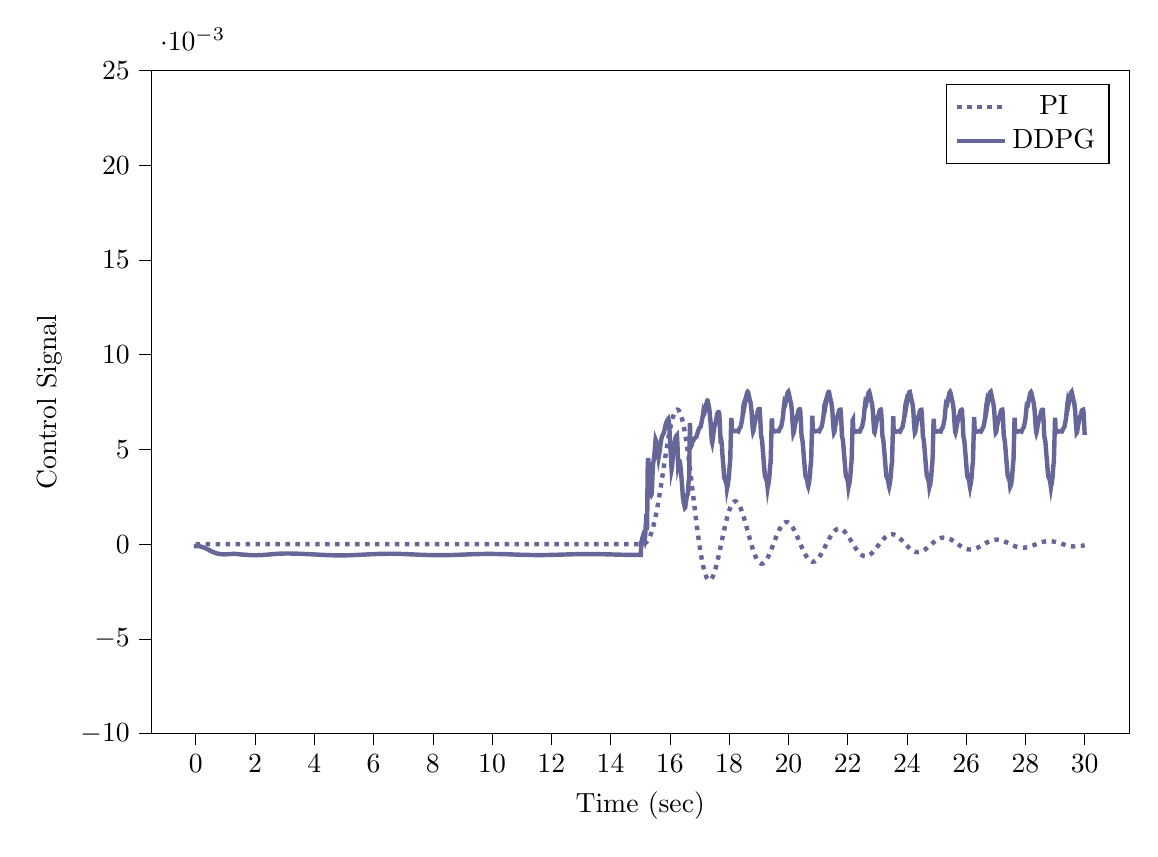
\begin{tikzpicture}

\definecolor{color0}{rgb}{0.12156862745098,0.466666666666667,0.705882352941177}
\definecolor{color1}{rgb}{1,0.498039215686275,0.0549019607843137}

\begin{axis}[
compat=newest,
tick align=outside,
tick pos=left,
x grid style={white!69.0196078431373!black},
xmin=-1.50000000000009, xmax=31.500000000002,
xtick style={color=black},
y grid style={white!69.0196078431373!black},
ymin=-0.01, ymax=0.025,
ytick style={color=black},
%yticklabel style={
%        /pgf/number format/.cd,
%        	fixed,
%        	fixed zerofill,
%         	precision=3,
%        /tikz/.cd
%},
scaled y ticks=true,
scaled y ticks=base 10:3,
width=14cm,
height=10cm,
xlabel=Time (sec),
ylabel=Control Signal
%y label style={at={(-0.2,0.5)}}
]

\addplot [ultra thick, blue!20!gray, dotted]
table {%
0 0
0.01 0
0.02 0
0.03 0
0.04 0
0.05 0
0.06 0
0.07 0
0.08 0
0.09 0
0.1 0
0.11 0
0.12 0
0.13 0
0.14 0
0.15 0
0.16 0
0.17 0
0.18 0
0.19 0
0.2 0
0.21 0
0.22 0
0.23 0
0.24 0
0.25 0
0.26 0
0.27 0
0.28 0
0.29 0
0.3 0
0.31 0
0.32 0
0.33 0
0.34 0
0.35 0
0.36 0
0.37 0
0.38 0
0.39 0
0.4 0
0.41 0
0.42 0
0.43 0
0.44 0
0.45 0
0.46 0
0.47 0
0.48 0
0.49 0
0.5 0
0.51 0
0.52 0
0.53 0
0.54 0
0.55 0
0.56 0
0.57 0
0.58 0
0.59 0
0.6 0
0.61 0
0.62 0
0.63 0
0.64 0
0.65 0
0.66 0
0.67 0
0.68 0
0.69 0
0.7 0
0.71 0
0.72 0
0.73 0
0.74 0
0.75 0
0.76 0
0.77 0
0.78 0
0.79 0
0.8 0
0.81 0
0.820000000000001 0
0.830000000000001 0
0.840000000000001 0
0.850000000000001 0
0.860000000000001 0
0.870000000000001 0
0.880000000000001 0
0.890000000000001 0
0.900000000000001 0
0.910000000000001 0
0.920000000000001 0
0.930000000000001 0
0.940000000000001 0
0.950000000000001 0
0.960000000000001 0
0.970000000000001 0
0.980000000000001 0
0.990000000000001 0
1 0
1.01 0
1.02 0
1.03 0
1.04 0
1.05 0
1.06 0
1.07 0
1.08 0
1.09 0
1.1 0
1.11 0
1.12 0
1.13 0
1.14 0
1.15 0
1.16 0
1.17 0
1.18 0
1.19 0
1.2 0
1.21 0
1.22 0
1.23 0
1.24 0
1.25 0
1.26 0
1.27 0
1.28 0
1.29 0
1.3 0
1.31 0
1.32 0
1.33 0
1.34 0
1.35 0
1.36 0
1.37 0
1.38 0
1.39 0
1.4 0
1.41 0
1.42 0
1.43 0
1.44 0
1.45 0
1.46 0
1.47 0
1.48 0
1.49 0
1.5 0
1.51 0
1.52 0
1.53 0
1.54 0
1.55 0
1.56 0
1.57 0
1.58 0
1.59 0
1.6 0
1.61 0
1.62 0
1.63 0
1.64 0
1.65 0
1.66 0
1.67 0
1.68 0
1.69 0
1.7 0
1.71 0
1.72 0
1.73 0
1.74 0
1.75 0
1.76 0
1.77 0
1.78 0
1.79 0
1.8 0
1.81 0
1.82 0
1.83 0
1.84 0
1.85 0
1.86 0
1.87 0
1.88 0
1.89 0
1.9 0
1.91 0
1.92 0
1.93 0
1.94 0
1.95 0
1.96 0
1.97 0
1.98 0
1.99 0
2 0
2.01 0
2.02 0
2.03 0
2.04 0
2.05 0
2.06 0
2.07 0
2.08 0
2.09 0
2.1 0
2.11 0
2.12 0
2.13 0
2.14 0
2.15 0
2.16 0
2.17 0
2.18 0
2.19 0
2.2 0
2.21 0
2.22 0
2.23 0
2.24 0
2.25 0
2.26 0
2.27 0
2.28 0
2.29 0
2.29999999999999 0
2.30999999999999 0
2.31999999999999 0
2.32999999999999 0
2.33999999999999 0
2.34999999999999 0
2.35999999999999 0
2.36999999999999 0
2.37999999999999 0
2.38999999999999 0
2.39999999999999 0
2.40999999999999 0
2.41999999999999 0
2.42999999999999 0
2.43999999999999 0
2.44999999999999 0
2.45999999999999 0
2.46999999999999 0
2.47999999999999 0
2.48999999999999 0
2.49999999999999 0
2.50999999999999 0
2.51999999999999 0
2.52999999999999 0
2.53999999999999 0
2.54999999999999 0
2.55999999999999 0
2.56999999999999 0
2.57999999999999 0
2.58999999999999 0
2.59999999999999 0
2.60999999999999 0
2.61999999999999 0
2.62999999999999 0
2.63999999999999 0
2.64999999999999 0
2.65999999999999 0
2.66999999999999 0
2.67999999999999 0
2.68999999999999 0
2.69999999999999 0
2.70999999999999 0
2.71999999999999 0
2.72999999999999 0
2.73999999999999 0
2.74999999999999 0
2.75999999999999 0
2.76999999999998 0
2.77999999999998 0
2.78999999999998 0
2.79999999999998 0
2.80999999999998 0
2.81999999999998 0
2.82999999999998 0
2.83999999999998 0
2.84999999999998 0
2.85999999999998 0
2.86999999999998 0
2.87999999999998 0
2.88999999999998 0
2.89999999999998 0
2.90999999999998 0
2.91999999999998 0
2.92999999999998 0
2.93999999999998 0
2.94999999999998 0
2.95999999999998 0
2.96999999999998 0
2.97999999999998 0
2.98999999999998 0
2.99999999999998 0
3.00999999999998 0
3.01999999999998 0
3.02999999999998 0
3.03999999999998 0
3.04999999999998 0
3.05999999999998 0
3.06999999999998 0
3.07999999999998 0
3.08999999999998 0
3.09999999999998 0
3.10999999999998 0
3.11999999999998 0
3.12999999999998 0
3.13999999999998 0
3.14999999999998 0
3.15999999999998 0
3.16999999999998 0
3.17999999999998 0
3.18999999999998 0
3.19999999999998 0
3.20999999999998 0
3.21999999999998 0
3.22999999999998 0
3.23999999999997 0
3.24999999999997 0
3.25999999999997 0
3.26999999999997 0
3.27999999999997 0
3.28999999999997 0
3.29999999999997 0
3.30999999999997 0
3.31999999999997 0
3.32999999999997 0
3.33999999999997 0
3.34999999999997 0
3.35999999999997 0
3.36999999999997 0
3.37999999999997 0
3.38999999999997 0
3.39999999999997 0
3.40999999999997 0
3.41999999999997 0
3.42999999999997 0
3.43999999999997 0
3.44999999999997 0
3.45999999999997 0
3.46999999999997 0
3.47999999999997 0
3.48999999999997 0
3.49999999999997 0
3.50999999999997 0
3.51999999999997 0
3.52999999999997 0
3.53999999999997 0
3.54999999999997 0
3.55999999999997 0
3.56999999999997 0
3.57999999999997 0
3.58999999999997 0
3.59999999999997 0
3.60999999999997 0
3.61999999999997 0
3.62999999999997 0
3.63999999999997 0
3.64999999999997 0
3.65999999999997 0
3.66999999999997 0
3.67999999999997 0
3.68999999999997 0
3.69999999999997 0
3.70999999999996 0
3.71999999999996 0
3.72999999999996 0
3.73999999999996 0
3.74999999999996 0
3.75999999999996 0
3.76999999999996 0
3.77999999999996 0
3.78999999999996 0
3.79999999999996 0
3.80999999999996 0
3.81999999999996 0
3.82999999999996 0
3.83999999999996 0
3.84999999999996 0
3.85999999999996 0
3.86999999999996 0
3.87999999999996 0
3.88999999999996 0
3.89999999999996 0
3.90999999999996 0
3.91999999999996 0
3.92999999999996 0
3.93999999999996 0
3.94999999999996 0
3.95999999999996 0
3.96999999999996 0
3.97999999999996 0
3.98999999999996 0
3.99999999999996 0
4.00999999999996 0
4.01999999999996 0
4.02999999999996 0
4.03999999999996 0
4.04999999999996 0
4.05999999999996 0
4.06999999999996 0
4.07999999999996 0
4.08999999999996 0
4.09999999999996 0
4.10999999999996 0
4.11999999999996 0
4.12999999999996 0
4.13999999999996 0
4.14999999999996 0
4.15999999999996 0
4.16999999999996 0
4.17999999999996 0
4.18999999999996 0
4.19999999999995 0
4.20999999999995 0
4.21999999999995 0
4.22999999999995 0
4.23999999999995 0
4.24999999999995 0
4.25999999999995 0
4.26999999999995 0
4.27999999999995 0
4.28999999999995 0
4.29999999999995 0
4.30999999999995 0
4.31999999999995 0
4.32999999999995 0
4.33999999999995 0
4.34999999999995 0
4.35999999999995 0
4.36999999999995 0
4.37999999999995 0
4.38999999999995 0
4.39999999999995 0
4.40999999999995 0
4.41999999999995 0
4.42999999999995 0
4.43999999999995 0
4.44999999999995 0
4.45999999999995 0
4.46999999999995 0
4.47999999999995 0
4.48999999999995 0
4.49999999999995 0
4.50999999999995 0
4.51999999999995 0
4.52999999999995 0
4.53999999999995 0
4.54999999999995 0
4.55999999999995 0
4.56999999999995 0
4.57999999999995 0
4.58999999999995 0
4.59999999999995 0
4.60999999999995 0
4.61999999999995 0
4.62999999999995 0
4.63999999999995 0
4.64999999999995 0
4.65999999999995 0
4.66999999999994 0
4.67999999999994 0
4.68999999999994 0
4.69999999999994 0
4.70999999999994 0
4.71999999999994 0
4.72999999999994 0
4.73999999999994 0
4.74999999999994 0
4.75999999999994 0
4.76999999999994 0
4.77999999999994 0
4.78999999999994 0
4.79999999999994 0
4.80999999999994 0
4.81999999999994 0
4.82999999999994 0
4.83999999999994 0
4.84999999999994 0
4.85999999999994 0
4.86999999999994 0
4.87999999999994 0
4.88999999999994 0
4.89999999999994 0
4.90999999999994 0
4.91999999999994 0
4.92999999999994 0
4.93999999999994 0
4.94999999999994 0
4.95999999999994 0
4.96999999999994 0
4.97999999999994 0
4.98999999999994 0
4.99999999999994 0
5.00999999999994 0
5.01999999999994 0
5.02999999999994 0
5.03999999999994 0
5.04999999999994 0
5.05999999999994 0
5.06999999999994 0
5.07999999999994 0
5.08999999999994 0
5.09999999999994 0
5.10999999999994 0
5.11999999999994 0
5.12999999999994 0
5.13999999999993 0
5.14999999999993 0
5.15999999999993 0
5.16999999999993 0
5.17999999999993 0
5.18999999999993 0
5.19999999999993 0
5.20999999999993 0
5.21999999999993 0
5.22999999999993 0
5.23999999999993 0
5.24999999999993 0
5.25999999999993 0
5.26999999999993 0
5.27999999999993 0
5.28999999999993 0
5.29999999999993 0
5.30999999999993 0
5.31999999999993 0
5.32999999999993 0
5.33999999999993 0
5.34999999999993 0
5.35999999999993 0
5.36999999999993 0
5.37999999999993 0
5.38999999999993 0
5.39999999999993 0
5.40999999999993 0
5.41999999999993 0
5.42999999999993 0
5.43999999999993 0
5.44999999999993 0
5.45999999999993 0
5.46999999999993 0
5.47999999999993 0
5.48999999999993 0
5.49999999999993 0
5.50999999999993 0
5.51999999999993 0
5.52999999999993 0
5.53999999999993 0
5.54999999999993 0
5.55999999999993 0
5.56999999999993 0
5.57999999999993 0
5.58999999999993 0
5.59999999999993 0
5.60999999999992 0
5.61999999999992 0
5.62999999999992 0
5.63999999999992 0
5.64999999999992 0
5.65999999999992 0
5.66999999999992 0
5.67999999999992 0
5.68999999999992 0
5.69999999999992 0
5.70999999999992 0
5.71999999999992 0
5.72999999999992 0
5.73999999999992 0
5.74999999999992 0
5.75999999999992 0
5.76999999999992 0
5.77999999999992 0
5.78999999999992 0
5.79999999999992 0
5.80999999999992 0
5.81999999999992 0
5.82999999999992 0
5.83999999999992 0
5.84999999999992 0
5.85999999999992 0
5.86999999999992 0
5.87999999999992 0
5.88999999999992 0
5.89999999999992 0
5.90999999999992 0
5.91999999999992 0
5.92999999999992 0
5.93999999999992 0
5.94999999999992 0
5.95999999999992 0
5.96999999999992 0
5.97999999999992 0
5.98999999999992 0
5.99999999999992 0
6.00999999999992 0
6.01999999999992 0
6.02999999999992 0
6.03999999999992 0
6.04999999999992 0
6.05999999999992 0
6.06999999999992 0
6.07999999999991 0
6.08999999999991 0
6.09999999999991 0
6.10999999999991 0
6.11999999999991 0
6.12999999999991 0
6.13999999999991 0
6.14999999999991 0
6.15999999999991 0
6.16999999999991 0
6.17999999999991 0
6.18999999999991 0
6.19999999999991 0
6.20999999999991 0
6.21999999999991 0
6.22999999999991 0
6.23999999999991 0
6.24999999999991 0
6.25999999999991 0
6.26999999999991 0
6.27999999999991 0
6.28999999999991 0
6.29999999999991 0
6.30999999999991 0
6.31999999999991 0
6.32999999999991 0
6.33999999999991 0
6.34999999999991 0
6.35999999999991 0
6.36999999999991 0
6.37999999999991 0
6.38999999999991 0
6.39999999999991 0
6.40999999999991 0
6.41999999999991 0
6.42999999999991 0
6.43999999999991 0
6.44999999999991 0
6.45999999999991 0
6.46999999999991 0
6.47999999999991 0
6.48999999999991 0
6.49999999999991 0
6.50999999999991 0
6.51999999999991 0
6.52999999999991 0
6.53999999999991 0
6.5499999999999 0
6.5599999999999 0
6.5699999999999 0
6.5799999999999 0
6.5899999999999 0
6.5999999999999 0
6.6099999999999 0
6.6199999999999 0
6.6299999999999 0
6.6399999999999 0
6.6499999999999 0
6.6599999999999 0
6.6699999999999 0
6.6799999999999 0
6.6899999999999 0
6.6999999999999 0
6.7099999999999 0
6.7199999999999 0
6.7299999999999 0
6.7399999999999 0
6.7499999999999 0
6.7599999999999 0
6.7699999999999 0
6.7799999999999 0
6.7899999999999 0
6.7999999999999 0
6.8099999999999 0
6.8199999999999 0
6.8299999999999 0
6.8399999999999 0
6.8499999999999 0
6.8599999999999 0
6.8699999999999 0
6.8799999999999 0
6.8899999999999 0
6.8999999999999 0
6.9099999999999 0
6.9199999999999 0
6.9299999999999 0
6.9399999999999 0
6.9499999999999 0
6.9599999999999 0
6.9699999999999 0
6.9799999999999 0
6.9899999999999 0
6.9999999999999 0
7.00999999999989 0
7.01999999999989 0
7.02999999999989 0
7.03999999999989 0
7.04999999999989 0
7.05999999999989 0
7.06999999999989 0
7.07999999999989 0
7.08999999999989 0
7.09999999999989 0
7.10999999999989 0
7.11999999999989 0
7.12999999999989 0
7.13999999999989 0
7.14999999999989 0
7.15999999999989 0
7.16999999999989 0
7.17999999999989 0
7.18999999999989 0
7.19999999999989 0
7.20999999999989 0
7.21999999999989 0
7.22999999999989 0
7.23999999999989 0
7.24999999999989 0
7.25999999999989 0
7.26999999999989 0
7.27999999999989 0
7.28999999999989 0
7.29999999999989 0
7.30999999999989 0
7.31999999999989 0
7.32999999999989 0
7.33999999999989 0
7.34999999999989 0
7.35999999999989 0
7.36999999999989 0
7.37999999999989 0
7.38999999999989 0
7.39999999999989 0
7.40999999999989 0
7.41999999999989 0
7.42999999999989 0
7.43999999999989 0
7.44999999999989 0
7.45999999999989 0
7.46999999999989 0
7.47999999999988 0
7.48999999999988 0
7.49999999999988 0
7.50999999999988 0
7.51999999999988 0
7.52999999999988 0
7.53999999999988 0
7.54999999999988 0
7.55999999999988 0
7.56999999999988 0
7.57999999999988 0
7.58999999999988 0
7.59999999999988 0
7.60999999999988 0
7.61999999999988 0
7.62999999999988 0
7.63999999999988 0
7.64999999999988 0
7.65999999999988 0
7.66999999999988 0
7.67999999999988 0
7.68999999999988 0
7.69999999999988 0
7.70999999999988 0
7.71999999999988 0
7.72999999999988 0
7.73999999999988 0
7.74999999999988 0
7.75999999999988 0
7.76999999999988 0
7.77999999999988 0
7.78999999999988 0
7.79999999999988 0
7.80999999999988 0
7.81999999999988 0
7.82999999999988 0
7.83999999999988 0
7.84999999999988 0
7.85999999999988 0
7.86999999999988 0
7.87999999999988 0
7.88999999999988 0
7.89999999999988 0
7.90999999999988 0
7.91999999999988 0
7.92999999999988 0
7.93999999999988 0
7.94999999999987 0
7.95999999999987 0
7.96999999999987 0
7.97999999999987 0
7.98999999999987 0
7.99999999999987 0
8.00999999999987 0
8.01999999999987 0
8.02999999999987 0
8.03999999999987 0
8.04999999999987 0
8.05999999999987 0
8.06999999999987 0
8.07999999999987 0
8.08999999999987 0
8.09999999999987 0
8.10999999999987 0
8.11999999999987 0
8.12999999999987 0
8.13999999999987 0
8.14999999999987 0
8.15999999999987 0
8.16999999999987 0
8.17999999999987 0
8.18999999999987 0
8.19999999999987 0
8.20999999999987 0
8.21999999999987 0
8.22999999999987 0
8.23999999999987 0
8.24999999999987 0
8.25999999999987 0
8.26999999999987 0
8.27999999999987 0
8.28999999999987 0
8.29999999999987 0
8.30999999999987 0
8.31999999999987 0
8.32999999999987 0
8.33999999999987 0
8.34999999999987 0
8.35999999999987 0
8.36999999999987 0
8.37999999999987 0
8.38999999999987 0
8.39999999999987 0
8.40999999999987 0
8.41999999999986 0
8.42999999999986 0
8.43999999999986 0
8.44999999999986 0
8.45999999999986 0
8.46999999999986 0
8.47999999999986 0
8.48999999999986 0
8.49999999999986 0
8.50999999999986 0
8.51999999999986 0
8.52999999999986 0
8.53999999999986 0
8.54999999999986 0
8.55999999999986 0
8.56999999999986 0
8.57999999999986 0
8.58999999999986 0
8.59999999999986 0
8.60999999999986 0
8.61999999999986 0
8.62999999999986 0
8.63999999999986 0
8.64999999999986 0
8.65999999999986 0
8.66999999999986 0
8.67999999999986 0
8.68999999999986 0
8.69999999999986 0
8.70999999999986 0
8.71999999999986 0
8.72999999999986 0
8.73999999999986 0
8.74999999999986 0
8.75999999999986 0
8.76999999999986 0
8.77999999999986 0
8.78999999999986 0
8.79999999999986 0
8.80999999999986 0
8.81999999999986 0
8.82999999999986 0
8.83999999999986 0
8.84999999999986 0
8.85999999999986 0
8.86999999999986 0
8.87999999999986 0
8.88999999999985 0
8.89999999999985 0
8.90999999999985 0
8.91999999999985 0
8.92999999999985 0
8.93999999999985 0
8.94999999999985 0
8.95999999999985 0
8.96999999999985 0
8.97999999999985 0
8.98999999999985 0
8.99999999999985 0
9.00999999999985 0
9.01999999999985 0
9.02999999999985 0
9.03999999999985 0
9.04999999999985 0
9.05999999999985 0
9.06999999999985 0
9.07999999999985 0
9.08999999999985 0
9.09999999999985 0
9.10999999999985 0
9.11999999999985 0
9.12999999999985 0
9.13999999999985 0
9.14999999999985 0
9.15999999999985 0
9.16999999999985 0
9.17999999999985 0
9.18999999999985 0
9.19999999999985 0
9.20999999999985 0
9.21999999999985 0
9.22999999999985 0
9.23999999999985 0
9.24999999999985 0
9.25999999999985 0
9.26999999999985 0
9.27999999999985 0
9.28999999999985 0
9.29999999999985 0
9.30999999999985 0
9.31999999999985 0
9.32999999999985 0
9.33999999999985 0
9.34999999999985 0
9.35999999999984 0
9.36999999999984 0
9.37999999999984 0
9.38999999999984 0
9.39999999999984 0
9.40999999999984 0
9.41999999999984 0
9.42999999999984 0
9.43999999999984 0
9.44999999999984 0
9.45999999999984 0
9.46999999999984 0
9.47999999999984 0
9.48999999999984 0
9.49999999999984 0
9.50999999999984 0
9.51999999999984 0
9.52999999999984 0
9.53999999999984 0
9.54999999999984 0
9.55999999999984 0
9.56999999999984 0
9.57999999999984 0
9.58999999999984 0
9.59999999999984 0
9.60999999999984 0
9.61999999999984 0
9.62999999999984 0
9.63999999999984 0
9.64999999999984 0
9.65999999999984 0
9.66999999999984 0
9.67999999999984 0
9.68999999999984 0
9.69999999999984 0
9.70999999999984 0
9.71999999999984 0
9.72999999999984 0
9.73999999999984 0
9.74999999999984 0
9.75999999999984 0
9.76999999999984 0
9.77999999999984 0
9.78999999999984 0
9.79999999999984 0
9.80999999999984 0
9.81999999999984 0
9.82999999999983 0
9.83999999999983 0
9.84999999999983 0
9.85999999999983 0
9.86999999999983 0
9.87999999999983 0
9.88999999999983 0
9.89999999999983 0
9.90999999999983 0
9.91999999999983 0
9.92999999999983 0
9.93999999999983 0
9.94999999999983 0
9.95999999999983 0
9.96999999999983 0
9.97999999999983 0
9.98999999999983 0
9.99999999999983 0
10.0099999999998 0
10.0199999999998 0
10.0299999999998 0
10.0399999999998 0
10.0499999999998 0
10.0599999999998 0
10.0699999999998 0
10.0799999999998 0
10.0899999999998 0
10.0999999999998 0
10.1099999999998 0
10.1199999999998 0
10.1299999999998 0
10.1399999999998 0
10.1499999999998 0
10.1599999999998 0
10.1699999999998 0
10.1799999999998 0
10.1899999999998 0
10.1999999999998 0
10.2099999999998 0
10.2199999999998 0
10.2299999999998 0
10.2399999999998 0
10.2499999999998 0
10.2599999999998 0
10.2699999999998 0
10.2799999999998 0
10.2899999999998 0
10.2999999999998 0
10.3099999999998 0
10.3199999999998 0
10.3299999999998 0
10.3399999999998 0
10.3499999999998 0
10.3599999999998 0
10.3699999999998 0
10.3799999999998 0
10.3899999999998 0
10.3999999999998 0
10.4099999999998 0
10.4199999999998 0
10.4299999999998 0
10.4399999999998 0
10.4499999999998 0
10.4599999999998 0
10.4699999999998 0
10.4799999999998 0
10.4899999999998 0
10.4999999999998 0
10.5099999999998 0
10.5199999999998 0
10.5299999999998 0
10.5399999999998 0
10.5499999999998 0
10.5599999999998 0
10.5699999999998 0
10.5799999999998 0
10.5899999999998 0
10.5999999999998 0
10.6099999999998 0
10.6199999999998 0
10.6299999999998 0
10.6399999999998 0
10.6499999999998 0
10.6599999999998 0
10.6699999999998 0
10.6799999999998 0
10.6899999999998 0
10.6999999999998 0
10.7099999999998 0
10.7199999999998 0
10.7299999999998 0
10.7399999999998 0
10.7499999999998 0
10.7599999999998 0
10.7699999999998 0
10.7799999999998 0
10.7899999999998 0
10.7999999999998 0
10.8099999999998 0
10.8199999999998 0
10.8299999999998 0
10.8399999999998 0
10.8499999999998 0
10.8599999999998 0
10.8699999999998 0
10.8799999999998 0
10.8899999999998 0
10.8999999999998 0
10.9099999999998 0
10.9199999999998 0
10.9299999999998 0
10.9399999999998 0
10.9499999999998 0
10.9599999999998 0
10.9699999999998 0
10.9799999999998 0
10.9899999999998 0
10.9999999999998 0
11.0099999999998 0
11.0199999999998 0
11.0299999999998 0
11.0399999999998 0
11.0499999999998 0
11.0599999999998 0
11.0699999999998 0
11.0799999999998 0
11.0899999999998 0
11.0999999999998 0
11.1099999999998 0
11.1199999999998 0
11.1299999999998 0
11.1399999999998 0
11.1499999999998 0
11.1599999999998 0
11.1699999999998 0
11.1799999999998 0
11.1899999999998 0
11.1999999999998 0
11.2099999999998 0
11.2199999999998 0
11.2299999999998 0
11.2399999999998 0
11.2499999999998 0
11.2599999999998 0
11.2699999999998 0
11.2799999999998 0
11.2899999999998 0
11.2999999999998 0
11.3099999999998 0
11.3199999999998 0
11.3299999999998 0
11.3399999999998 0
11.3499999999998 0
11.3599999999998 0
11.3699999999998 0
11.3799999999998 0
11.3899999999998 0
11.3999999999998 0
11.4099999999998 0
11.4199999999998 0
11.4299999999998 0
11.4399999999998 0
11.4499999999998 0
11.4599999999998 0
11.4699999999998 0
11.4799999999998 0
11.4899999999998 0
11.4999999999998 0
11.5099999999998 0
11.5199999999998 0
11.5299999999998 0
11.5399999999998 0
11.5499999999998 0
11.5599999999998 0
11.5699999999998 0
11.5799999999998 0
11.5899999999998 0
11.5999999999998 0
11.6099999999998 0
11.6199999999998 0
11.6299999999998 0
11.6399999999998 0
11.6499999999998 0
11.6599999999998 0
11.6699999999998 0
11.6799999999998 0
11.6899999999998 0
11.6999999999998 0
11.7099999999998 0
11.7199999999998 0
11.7299999999998 0
11.7399999999998 0
11.7499999999998 0
11.7599999999998 0
11.7699999999998 0
11.7799999999998 0
11.7899999999998 0
11.7999999999998 0
11.8099999999998 0
11.8199999999998 0
11.8299999999998 0
11.8399999999998 0
11.8499999999998 0
11.8599999999998 0
11.8699999999998 0
11.8799999999998 0
11.8899999999998 0
11.8999999999998 0
11.9099999999998 0
11.9199999999998 0
11.9299999999998 0
11.9399999999998 0
11.9499999999998 0
11.9599999999998 0
11.9699999999998 0
11.9799999999998 0
11.9899999999998 0
11.9999999999998 0
12.0099999999998 0
12.0199999999998 0
12.0299999999998 0
12.0399999999998 0
12.0499999999998 0
12.0599999999998 0
12.0699999999998 0
12.0799999999998 0
12.0899999999998 0
12.0999999999998 0
12.1099999999998 0
12.1199999999998 0
12.1299999999998 0
12.1399999999998 0
12.1499999999998 0
12.1599999999998 0
12.1699999999998 0
12.1799999999998 0
12.1899999999998 0
12.1999999999998 0
12.2099999999998 0
12.2199999999998 0
12.2299999999998 0
12.2399999999998 0
12.2499999999998 0
12.2599999999998 0
12.2699999999998 0
12.2799999999998 0
12.2899999999998 0
12.2999999999998 0
12.3099999999998 0
12.3199999999998 0
12.3299999999998 0
12.3399999999998 0
12.3499999999998 0
12.3599999999998 0
12.3699999999998 0
12.3799999999998 0
12.3899999999998 0
12.3999999999998 0
12.4099999999998 0
12.4199999999998 0
12.4299999999998 0
12.4399999999998 0
12.4499999999998 0
12.4599999999998 0
12.4699999999998 0
12.4799999999998 0
12.4899999999998 0
12.4999999999998 0
12.5099999999998 0
12.5199999999998 0
12.5299999999998 0
12.5399999999998 0
12.5499999999998 0
12.5599999999998 0
12.5699999999998 0
12.5799999999998 0
12.5899999999998 0
12.5999999999998 0
12.6099999999998 0
12.6199999999998 0
12.6299999999998 0
12.6399999999998 0
12.6499999999998 0
12.6599999999998 0
12.6699999999998 0
12.6799999999998 0
12.6899999999998 0
12.6999999999998 0
12.7099999999998 0
12.7199999999998 0
12.7299999999998 0
12.7399999999998 0
12.7499999999998 0
12.7599999999998 0
12.7699999999998 0
12.7799999999998 0
12.7899999999998 0
12.7999999999998 0
12.8099999999998 0
12.8199999999998 0
12.8299999999998 0
12.8399999999998 0
12.8499999999998 0
12.8599999999998 0
12.8699999999998 0
12.8799999999998 0
12.8899999999998 0
12.8999999999998 0
12.9099999999998 0
12.9199999999998 0
12.9299999999998 0
12.9399999999998 0
12.9499999999998 0
12.9599999999998 0
12.9699999999998 0
12.9799999999998 0
12.9899999999998 0
12.9999999999998 0
13.0099999999998 0
13.0199999999998 0
13.0299999999998 0
13.0399999999998 0
13.0499999999998 0
13.0599999999998 0
13.0699999999998 0
13.0799999999998 0
13.0899999999998 0
13.0999999999998 0
13.1099999999998 0
13.1199999999998 0
13.1299999999998 0
13.1399999999998 0
13.1499999999998 0
13.1599999999998 0
13.1699999999998 0
13.1799999999998 0
13.1899999999998 0
13.1999999999998 0
13.2099999999998 0
13.2199999999998 0
13.2299999999998 0
13.2399999999998 0
13.2499999999998 0
13.2599999999998 0
13.2699999999998 0
13.2799999999998 0
13.2899999999998 0
13.2999999999998 0
13.3099999999998 0
13.3199999999998 0
13.3299999999998 0
13.3399999999998 0
13.3499999999998 0
13.3599999999998 0
13.3699999999998 0
13.3799999999998 0
13.3899999999998 0
13.3999999999998 0
13.4099999999998 0
13.4199999999998 0
13.4299999999998 0
13.4399999999998 0
13.4499999999998 0
13.4599999999998 0
13.4699999999998 0
13.4799999999998 0
13.4899999999998 0
13.4999999999998 0
13.5099999999998 0
13.5199999999998 0
13.5299999999998 0
13.5399999999998 0
13.5499999999998 0
13.5599999999998 0
13.5699999999998 0
13.5799999999998 0
13.5899999999998 0
13.5999999999998 0
13.6099999999998 0
13.6199999999998 0
13.6299999999998 0
13.6399999999998 0
13.6499999999998 0
13.6599999999998 0
13.6699999999998 0
13.6799999999998 0
13.6899999999998 0
13.6999999999998 0
13.7099999999998 0
13.7199999999998 0
13.7299999999998 0
13.7399999999998 0
13.7499999999998 0
13.7599999999998 0
13.7699999999998 0
13.7799999999998 0
13.7899999999998 0
13.7999999999998 0
13.8099999999998 0
13.8199999999997 0
13.8299999999997 0
13.8399999999997 0
13.8499999999997 0
13.8599999999997 0
13.8699999999997 0
13.8799999999997 0
13.8899999999997 0
13.8999999999997 0
13.9099999999997 0
13.9199999999997 0
13.9299999999997 0
13.9399999999997 0
13.9499999999997 0
13.9599999999997 0
13.9699999999997 0
13.9799999999997 0
13.9899999999997 0
13.9999999999997 0
14.0099999999997 0
14.0199999999997 0
14.0299999999997 0
14.0399999999997 0
14.0499999999997 0
14.0599999999997 0
14.0699999999997 0
14.0799999999997 0
14.0899999999997 0
14.0999999999997 0
14.1099999999997 0
14.1199999999997 0
14.1299999999997 0
14.1399999999997 0
14.1499999999997 0
14.1599999999997 0
14.1699999999997 0
14.1799999999997 0
14.1899999999997 0
14.1999999999997 0
14.2099999999997 0
14.2199999999997 0
14.2299999999997 0
14.2399999999997 0
14.2499999999997 0
14.2599999999997 0
14.2699999999997 0
14.2799999999997 0
14.2899999999997 0
14.2999999999997 0
14.3099999999997 0
14.3199999999997 0
14.3299999999997 0
14.3399999999997 0
14.3499999999997 0
14.3599999999997 0
14.3699999999997 0
14.3799999999997 0
14.3899999999997 0
14.3999999999997 0
14.4099999999997 0
14.4199999999997 0
14.4299999999997 0
14.4399999999997 0
14.4499999999997 0
14.4599999999997 0
14.4699999999997 0
14.4799999999997 0
14.4899999999997 0
14.4999999999997 0
14.5099999999997 0
14.5199999999997 0
14.5299999999997 0
14.5399999999997 0
14.5499999999997 0
14.5599999999997 0
14.5699999999997 0
14.5799999999997 0
14.5899999999997 0
14.5999999999997 0
14.6099999999997 0
14.6199999999997 0
14.6299999999997 0
14.6399999999997 0
14.6499999999997 0
14.6599999999997 0
14.6699999999997 0
14.6799999999997 0
14.6899999999997 0
14.6999999999997 0
14.7099999999997 0
14.7199999999997 0
14.7299999999997 0
14.7399999999997 0
14.7499999999997 0
14.7599999999997 0
14.7699999999997 0
14.7799999999997 0
14.7899999999997 0
14.7999999999997 0
14.8099999999997 0
14.8199999999997 0
14.8299999999997 0
14.8399999999997 0
14.8499999999997 0
14.8599999999997 0
14.8699999999997 0
14.8799999999997 0
14.8899999999997 0
14.8999999999997 0
14.9099999999997 0
14.9199999999997 0
14.9299999999997 0
14.9399999999997 0
14.9499999999997 0
14.9599999999997 0
14.9699999999997 0
14.9799999999997 0
14.9899999999997 0
14.9999999999997 -5.70830428551306e-18
15.0099999999997 3.16582986401435e-09
15.0199999999997 6.4095514367861e-08
15.0299999999997 2.52254773417937e-07
15.0399999999997 6.38207432399233e-07
15.0499999999997 1.29283722412152e-06
15.0599999999997 2.28732792301784e-06
15.0699999999997 3.693046053926e-06
15.0799999999997 5.58144736188225e-06
15.0899999999997 8.02397056797939e-06
15.0999999999997 1.10919196044069e-05
15.1099999999997 1.48563421017371e-05
15.1199999999997 1.93879048791312e-05
15.1299999999997 2.47567669712718e-05
15.1399999999997 3.10324507935009e-05
15.1499999999997 3.82837120408192e-05
15.1599999999997 4.6578408885806e-05
15.1699999999997 5.59833710026022e-05
15.1799999999997 6.65642689053346e-05
15.1899999999997 7.83854840523476e-05
15.1999999999997 9.15099801333487e-05
15.2099999999997 0.000105999175924994
15.2199999999997 0.000121912820071709
15.2299999999997 0.00013930886812241
15.2399999999997 0.000158243362129602
15.2499999999997 0.00017877031309584
15.2599999999997 0.000200941586531816
15.2699999999997 0.000224806791372187
15.2799999999997 0.000250413172477774
15.2899999999997 0.000277805506936627
15.2999999999997 0.000307026004361612
15.3099999999997 0.000338114211367584
15.3199999999997 0.000371106920398045
15.3299999999997 0.000406038083058335
15.3399999999997 0.000442938728100153
15.3499999999997 0.000481836884190298
15.3599999999997 0.000522757507585529
15.3699999999997 0.000565722414824199
15.3799999999997 0.000610750220534986
15.3899999999997 0.000657856280452334
15.3999999999997 0.000707052639718459
15.4099999999997 0.000758347986541834
15.4199999999997 0.000811747611272125
15.4299999999997 0.000867253370942678
15.4399999999997 0.00092486365912912
15.4499999999997 0.000984573381906295
15.4599999999997 0.00104637393886669
15.4699999999997 0.00111025320982344
15.4799999999997 0.00117619554711337
15.4899999999997 0.00124418177332968
15.4999999999997 0.0013141891851666
15.5099999999997 0.0013861915622454
15.5199999999997 0.00146015918165394
15.5299999999997 0.00153605883797134
15.5399999999997 0.00161385386873338
15.5499999999997 0.00169350418528655
15.5599999999997 0.00177496630897149
15.5699999999997 0.0018581934125681
15.5799999999997 0.00194313536679334
15.5899999999997 0.00202973879104507
15.5999999999997 0.0021179470684773
15.6099999999997 0.00220770045134358
15.6199999999997 0.00229893617131797
15.6299999999997 0.00239158846621547
15.6399999999997 0.00248558865586301
15.6499999999997 0.00258086522244214
15.6599999999997 0.00267734389517635
15.6699999999997 0.00277494773922958
15.6799999999997 0.00287359724867718
15.6899999999997 0.00297321044340427
15.6999999999997 0.00307370296541647
15.7099999999997 0.00317498818466556
15.7199999999997 0.00327697729875354
15.7299999999997 0.00337957949756025
15.7399999999997 0.00348270203615616
15.7499999999997 0.00358625035230324
15.7599999999997 0.00369012818676533
15.7699999999997 0.00379423770625431
15.7799999999997 0.00389847962890953
15.7899999999997 0.00400275335190738
15.7999999999997 0.00410695708122278
15.8099999999997 0.00421098796303527
15.8199999999997 0.00431474221716035
15.8299999999997 0.00441811527302718
15.8399999999997 0.00452100190515299
15.8499999999997 0.00462329637056947
15.8599999999997 0.00472489254720257
15.8699999999997 0.00482568407301256
15.8799999999997 0.00492556448569898
15.8899999999997 0.00502442736277578
15.8999999999997 0.00512216646182205
15.9099999999997 0.00521867586071333
15.9199999999997 0.00531385009763976
15.9299999999997 0.00540758431047893
15.9399999999997 0.00549977437538312
15.9499999999997 0.00559031704652859
15.9599999999997 0.00567911009250827
15.9699999999997 0.00576605243241056
15.9799999999997 0.00585104427054608
15.9899999999997 0.00593398722963875
15.9999999999997 0.00601478448230053
16.0099999999997 0.00609334088061049
16.0199999999997 0.00616956308362307
16.0299999999997 0.00624335968263212
16.0399999999997 0.00631464132402082
16.0499999999997 0.00638332082952973
16.0599999999997 0.00644931331403872
16.0699999999997 0.00651253658457738
16.0799999999997 0.00657291070242792
16.0899999999997 0.00663035835768284
16.0999999999997 0.00668480497462583
16.1099999999997 0.00673617881364848
16.1199999999997 0.00678441106957241
16.1299999999997 0.00682943596625108
16.1399999999997 0.00687119084733061
16.1499999999997 0.00690961626305432
16.1599999999997 0.00694465605300132
16.1699999999997 0.00697625742465436
16.1799999999997 0.00700437102769891
16.1899999999997 0.00702895102396017
16.1999999999997 0.00704995515289139
16.2099999999997 0.00706734479253259
16.2199999999997 0.00708108501586492
16.2299999999997 0.00709114464249198
16.2399999999997 0.00709749628558605
16.2499999999997 0.00710011639404302
16.2599999999997 0.00709898528979656
16.2699999999997 0.00709408720024824
16.2799999999997 0.00708541028577672
16.2899999999997 0.0070729466622958
16.2999999999997 0.00705669241883721
16.3099999999998 0.00703664763014089
16.3199999999998 0.00701281640524231
16.3299999999998 0.0069852069156603
16.3399999999998 0.00695383122659498
16.3499999999998 0.00691870538971264
16.3599999999998 0.00687984948452364
16.3699999999998 0.00683728757929552
16.3799999999998 0.00679104758724806
16.3899999999998 0.0067411613294634
16.3999999999998 0.00668766450290055
16.4099999999998 0.00663059664364932
16.4199999999998 0.00657000108586618
16.4299999999998 0.00650592491690309
16.4399999999998 0.00643841892296777
16.4499999999998 0.0063675375356487
16.4599999999998 0.00629333877213488
16.4699999999998 0.0062158841710539
16.4799999999998 0.00613523872755749
16.4899999999998 0.00605147081876108
16.4999999999998 0.0059646521199287
16.5099999999998 0.00587485752915641
16.5199999999998 0.00578216508273342
16.5299999999998 0.00568665614921501
16.5399999999998 0.00558841483809792
16.5499999999998 0.00548752799266845
16.5599999999998 0.00538408522485179
16.5699999999998 0.00527817881166705
16.5799999999998 0.00516990358876992
16.5899999999998 0.00505935684116751
16.5999999999998 0.00494663819120494
16.6099999999998 0.00483184948393927
16.6199999999998 0.00471509467002372
16.6299999999998 0.00459647968623776
16.6399999999998 0.00447611233380098
16.6499999999998 0.00435410215889557
16.6599999999998 0.00423056031816772
16.6699999999998 0.00410559945558449
16.6799999999998 0.0039793335736597
16.6899999999998 0.00385187790294693
16.6999999999998 0.0037233487702446
16.7099999999998 0.00359386346567685
16.7199999999998 0.00346354010881452
16.7299999999998 0.00333249751400318
16.7399999999998 0.00320085505506547
16.7499999999998 0.00306873252954454
16.7599999999998 0.00293625002265784
16.7699999999998 0.00280352777112922
16.7799999999998 0.00267068602706632
16.7899999999998 0.00253784492204737
16.7999999999998 0.00240512433154895
16.8099999999998 0.0022726437400331
16.8199999999998 0.00214052210669016
16.8299999999998 0.00200887773203881
16.8399999999998 0.0018778281255647
16.8499999999998 0.00174748987455897
16.8599999999998 0.00161797851431455
16.8699999999998 0.00148940839983686
16.8799999999998 0.00136189257922293
16.8899999999998 0.0012355426688601
16.8999999999998 0.00111046873059425
16.9099999999998 0.000986779151013352
16.9199999999998 0.000864580522991584
16.9299999999998 0.000743977529615421
16.9399999999998 0.00062507283066071
16.9499999999999 0.000507966951730065
16.9599999999999 0.000392758176205831
16.9699999999999 0.000279542440152602
16.9799999999999 0.000168413230164284
16.9899999999999 5.94614844141978e-05
16.9999999999999 -4.72245030196086e-05
17.0099999999999 -0.000151559174449319
17.0199999999999 -0.000253459797389182
17.0299999999999 -0.000352846549784439
17.0399999999999 -0.000449642601562814
17.0499999999999 -0.000543774192419465
17.0599999999999 -0.000635170705749957
17.0699999999999 -0.000723764738651565
17.0799999999999 -0.000809492167918202
17.0899999999999 -0.000892292211959066
17.0999999999999 -0.000972107488117029
17.1099999999999 -0.0010488840634568
17.1199999999999 -0.00112257151124656
17.1299999999999 -0.00119312295231248
17.1399999999999 -0.00126049509542793
17.1499999999999 -0.0013246482735962
17.1599999999999 -0.00138554647590818
17.1699999999999 -0.00144315737501954
17.1799999999999 -0.00149745235035225
17.1899999999999 -0.00154840650570783
17.1999999999999 -0.00159599868359749
17.2099999999999 -0.00164021182107533
17.2199999999999 -0.00168103230020265
17.2299999999999 -0.00171845024788507
17.2399999999999 -0.0017524595433233
17.2499999999999 -0.00178305780999191
17.2599999999999 -0.00181024640320835
17.2699999999999 -0.00183403039332332
17.2799999999999 -0.00185441854397552
17.2899999999999 -0.00187142328690473
17.2999999999999 -0.0018850606942511
17.3099999999999 -0.0018953504428999
17.3199999999999 -0.00190231577643821
17.3299999999999 -0.00190598346302608
17.3399999999999 -0.00190638374924856
17.3499999999999 -0.00190355031001957
17.3599999999999 -0.00189752019463488
17.3699999999999 -0.00188833376904088
17.3799999999999 -0.00187603465426445
17.3899999999999 -0.00186066966138258
17.3999999999999 -0.00184228872291376
17.4099999999999 -0.00182094482078316
17.4199999999999 -0.0017966939109632
17.4299999999999 -0.00176959484489591
17.4399999999999 -0.00173970928780674
17.4499999999999 -0.00170710163402465
17.4599999999999 -0.00167183891942532
17.4699999999999 -0.0016339907311215
17.4799999999999 -0.0015936291145262
17.4899999999999 -0.00155082848311854
17.4999999999999 -0.00150566551713047
17.5099999999999 -0.0014582190537429
17.5199999999999 -0.00140856999297742
17.5299999999999 -0.0013568011936934
17.5399999999999 -0.0013029977059424
17.5499999999999 -0.00124724664579199
17.5599999999999 -0.00118963588752606
17.5699999999999 -0.0011302548624594
17.5799999999999 -0.00106919443703924
17.59 -0.0010065467926173
17.6 -0.000942405306051211
17.61 -0.000876864430672182
17.62 -0.000810019577375527
17.63 -0.000741966995723295
17.64 -0.000672803655032476
17.65 -0.000602627125476129
17.66 -0.000531535459257622
17.67 -0.000459627071943747
17.68 -0.000387000624057039
17.69 -0.000313754903038329
17.7 -0.000239988705698012
17.71 -0.000165800721277174
17.72 -9.12894152468257e-05
17.73 -1.6552913971756e-05
17.74 5.83111096318273e-05
17.75 0.0001332055493174
17.76 0.00020803397747909
17.77 0.000282700755746424
17.78 0.000357111144076837
17.79 0.000431171408222327
17.8 0.000504788925448369
17.81 0.000577872288385991
17.82 0.000650331406899256
17.83 0.000722077607594058
17.84 0.000793023731604421
17.85 0.000863084230077375
17.86 0.000932175256780941
17.87 0.0010002147583934
17.88 0.00106712256216795
17.89 0.00113282046087706
17.9 0.00119723229494529
17.91 0.00126028403168271
17.92 0.00132190384153528
17.93 0.00138202217127153
17.94 0.00144057181402991
17.95 0.00149748797615476
17.96 0.00155270834075261
17.97 0.0016061731279052
17.98 0.0016578251514791
17.99 0.00170760987247642
18 0.00175547544887438
18.01 0.00180137278190664
18.02 0.00184525555874129
18.03 0.0018870802915159
18.04 0.00192680635269175
18.05 0.00196439600669292
18.06 0.00199981466375061
18.07 0.00203303060637553
18.08 0.00206401495483193
18.09 0.00209274181276756
18.1 0.00211918828055268
18.11 0.00214333446487668
18.12 0.0021651634846102
18.13 0.00218466147294417
18.14 0.0022018175758226
18.15 0.00221662394668934
18.16 0.00222907573757446
18.17 0.00223917108654924
18.18 0.00224691110158371
18.19 0.00225229983958907
18.2 0.00225534428540784
18.21 0.00225605432503161
18.22 0.00225444271462159
18.2300000000001 0.00225052504699032
18.2400000000001 0.00224431971484416
18.2500000000001 0.00223584787076598
18.2600000000001 0.0022251333840157
18.2700000000001 0.00221220279422165
18.2800000000001 0.00219708526203617
18.2900000000001 0.00217981251683245
18.3000000000001 0.00216041880287397
18.3100000000001 0.00213894081976098
18.3200000000001 0.00211541766148802
18.3300000000001 0.00208989075340664
18.3400000000001 0.00206240378644499
18.3500000000001 0.00203300264889083
18.3600000000001 0.00200173535584255
18.3700000000001 0.00196865197643489
18.3800000000001 0.00193380509699219
18.3900000000001 0.00189724879452465
18.4000000000001 0.00185903875145192
18.4100000000001 0.00181923240051995
18.4200000000001 0.00177788884048817
18.4300000000001 0.00173506875058237
18.4400000000001 0.001690834303736
18.4500000000001 0.00164524907866692
18.4600000000001 0.00159837797085722
18.4700000000001 0.00155028710251569
18.4800000000001 0.00150104373161316
18.4900000000001 0.00145071616008754
18.5000000000001 0.0013993736413311
18.5100000000001 0.00134708628703775
18.5200000000001 0.0012939249735243
18.5300000000001 0.00123996124769647
18.5400000000001 0.0011852672327048
18.5500000000001 0.00112991553342673
18.5600000000001 0.00107397914189023
18.5700000000001 0.00101753134275305
18.5800000000001 0.000960645618953039
18.5900000000001 0.000903395557644
18.6000000000001 0.00084585475653117
18.6100000000001 0.000788096730719876
18.6200000000001 0.000730194820189504
18.6300000000001 0.00067222209800447
18.6400000000001 0.000614251279371719
18.6500000000001 0.000556354631654228
18.6600000000001 0.000498603885446795
18.6700000000001 0.000441070146819918
18.6800000000001 0.00038382381083472
18.6900000000001 0.000326934476431073
18.7000000000001 0.000270470862788109
18.7100000000001 0.000214500727253764
18.7200000000001 0.00015909078493602
18.7300000000001 0.000104306630053445
18.7400000000001 5.021265913101e-05
18.7500000000001 -3.12800387165861e-06
18.7600000000001 -5.56535831460837e-05
18.7700000000001 -0.000107303741790825
18.7800000000001 -0.000158019605950413
18.7900000000001 -0.000207743852869671
18.8000000000001 -0.000256420774938268
18.8100000000001 -0.000303996341342167
18.8200000000001 -0.00035041825725647
18.8300000000001 -0.000395636020517412
18.8400000000001 -0.000439600975714877
18.8500000000001 -0.000482266365490447
18.8600000000001 -0.000523587379145296
18.8700000000002 -0.00056352119942967
18.8800000000002 -0.000602027045363843
18.8900000000002 -0.000639066212665945
18.9000000000002 -0.000674602111316766
18.9100000000002 -0.000708600300225057
18.9200000000002 -0.0007410285189606
18.9300000000002 -0.000771856716523908
18.9400000000002 -0.000801057152302327
18.9500000000002 -0.000828604505423008
18.9600000000002 -0.000854475519022425
18.9700000000002 -0.00087864923234182
18.9800000000002 -0.000901106994815698
18.9900000000002 -0.000921832477136327
19.0000000000002 -0.00094081167931275
19.0100000000002 -0.000958032935725497
19.0200000000002 -0.000973486917186671
19.0300000000002 -0.00098716663001893
19.0400000000002 -0.000999067412170318
19.0500000000002 -0.00100918692638559
19.0600000000002 -0.00101752515045824
19.0700000000002 -0.00102408436459094
19.0800000000002 -0.00102886914315786
19.0900000000002 -0.00103188634197821
19.1000000000002 -0.00103314504439477
19.1100000000002 -0.00103265655735996
19.1200000000002 -0.00103043438426745
19.1300000000002 -0.00102649419644822
19.1400000000002 -0.00102085380221011
19.1500000000002 -0.00101353311151227
19.1600000000002 -0.00100455409911726
19.1700000000002 -0.000993940765311762
19.1800000000002 -0.000981719094259131
19.1900000000002 -0.00096791701005008
19.2000000000002 -0.000952564331044898
19.2100000000002 -0.000935692721632995
19.2200000000002 -0.000917335640454701
19.2300000000002 -0.000897528288409929
19.2400000000002 -0.000876307554371287
19.2500000000002 -0.000853711959022402
19.2600000000002 -0.000829781596923679
19.2700000000002 -0.000804558076904478
19.2800000000002 -0.00077808495330504
19.2900000000002 -0.00075040699763155
19.3000000000002 -0.000721569844307936
19.3100000000002 -0.000691620405692086
19.3200000000002 -0.000660606800454154
19.3300000000002 -0.000628578281981576
19.3400000000002 -0.000595585166538142
19.3500000000002 -0.000561678761029385
19.3600000000002 -0.000526911290304492
19.3700000000002 -0.000491335823976119
19.3800000000002 -0.000455006202773336
19.3900000000002 -0.000417976964465901
19.4000000000002 -0.000380303269414035
19.4100000000002 -0.000342040825808863
19.4200000000002 -0.00030324581467651
19.4300000000002 -0.000263974814724636
19.4400000000002 -0.000224284727113777
19.4500000000002 -0.000184232700239002
19.4600000000002 -0.000143876054609051
19.4700000000002 -0.000103272207911281
19.4800000000002 -6.24786003516973e-05
19.4900000000002 -2.1552620359675e-05
19.5000000000002 1.94484692544224e-05
19.5100000000003 6.04676045989079e-05
19.5200000000003 0.000101447993369119
19.5300000000003 0.000142333186797615
19.5400000000003 0.000183067150799313
19.5500000000003 0.000223594336226558
19.5600000000003 0.000263859748149506
19.5700000000003 0.00030380901408005
19.5800000000003 0.000343388451057392
19.5900000000003 0.000382545131516784
19.6000000000003 0.000421226947863121
19.6100000000003 0.000459382675674416
19.6200000000003 0.000496962035461117
19.6300000000003 0.000533915752909619
19.6400000000003 0.000570195617541221
19.6500000000003 0.000605754539718526
19.6600000000003 0.000640546605935019
19.6700000000003 0.000674527132325168
19.6800000000003 0.000707652716334761
19.6900000000003 0.000739881286494044
19.7000000000003 0.00077117215023859
19.7100000000003 0.000801486039724938
19.7200000000003 0.000830785155591172
19.7300000000003 0.000859033208614452
19.7400000000003 0.00088619545922052
19.7500000000003 0.000912238754802217
19.7600000000003 0.000937131564806279
19.7700000000003 0.000960844013549857
19.7800000000003 0.000983347910730289
19.7900000000003 0.00100461677959239
19.8000000000003 0.0010246259873914
19.8100000000003 0.00104335280208421
19.8200000000003 0.00106077605908662
19.8300000000003 0.00107687639823602
19.8400000000003 0.00109163628038271
19.8500000000003 0.0011050400015626
19.8600000000003 0.00111707370475002
19.8700000000003 0.00112772538918481
19.8800000000003 0.00113698491727372
19.8900000000003 0.00114484401907031
19.9000000000003 0.00115129629433905
19.9100000000003 0.00115633721221385
19.9200000000003 0.00115996410846278
19.9300000000003 0.00116217618037468
19.9400000000003 0.00116297447928581
19.9500000000003 0.00116236190076764
19.9600000000003 0.00116034317250002
19.9700000000003 0.00115692483985667
19.9800000000003 0.00115211524826048
19.9900000000003 0.00114592452616002
20.0000000000003 0.00113836456335866
20.0100000000003 0.00112944898744659
20.0200000000003 0.00111919313840137
20.0300000000003 0.00110761404118386
20.0400000000003 0.00109473037628932
20.0500000000003 0.00108056244832308
20.0600000000003 0.00106513215265021
20.0700000000003 0.00104846294016852
20.0800000000003 0.00103057978068462
20.0900000000003 0.00101150912459892
20.1000000000003 0.000991278860149532
20.1100000000003 0.00096991827251846
20.1200000000003 0.000947458000166819
20.1300000000003 0.000923929989656607
20.1400000000003 0.000899367449041313
20.1500000000004 0.000873804799905687
20.1600000000004 0.000847277628140366
20.1700000000004 0.000819823049493038
20.1800000000004 0.000791479166380546
20.1900000000004 0.000762284604516693
20.2000000000004 0.000732278970220634
20.2100000000004 0.000701502775771606
20.2200000000004 0.000669997375372842
20.2300000000004 0.000637804918027438
20.2400000000004 0.00060496828767523
20.2500000000004 0.000571531043191945
20.2600000000004 0.000537537358184712
20.2700000000004 0.000503031960560795
20.2800000000004 0.000468060071877184
20.2900000000004 0.000432667346497539
20.3000000000004 0.000396899810597034
20.3100000000004 0.000360803801065761
20.3200000000004 0.00032442590436718
20.3300000000004 0.000287812895414107
20.3400000000004 0.000251011676527094
20.3500000000004 0.000214069216543187
20.3600000000004 0.000177032490143798
20.3700000000004 0.000139948417472626
20.3800000000004 0.000102863804114195
20.3900000000004 6.58252815027688e-05
20.4000000000004 2.88792478339467e-05
20.4100000000004 -7.92819045066531e-06
20.4200000000004 -4.45512765368985e-05
20.4300000000004 -8.09446603996111e-05
20.4400000000004 -0.000117063455184525
20.4500000000004 -0.000152863292743147
20.4600000000004 -0.000188300378254848
20.4700000000004 -0.000223331543871137
20.4800000000004 -0.000257914301319138
20.4900000000004 -0.000292006893402279
20.5000000000004 -0.000325568344337795
20.5100000000004 -0.000358558508872617
20.5200000000004 -0.000390938120120638
20.5300000000004 -0.000422668836066032
20.5400000000004 -0.000453713284679812
20.5500000000004 -0.000484035107597448
20.5600000000004 -0.000513599002308912
20.5700000000004 -0.000542370762812995
20.5800000000004 -0.000570317318690812
20.5900000000004 -0.000597406772554821
20.6000000000004 -0.000623608435832152
20.6100000000004 -0.000648892862842647
20.6200000000004 -0.000673231883134423
20.6300000000004 -0.000696598632041711
20.6400000000004 -0.000718967579431033
20.6500000000004 -0.000740314556604718
20.6600000000004 -0.000760616781331157
20.6700000000004 -0.000779852880973611
20.6800000000004 -0.000798002913689881
20.6900000000004 -0.000815048387676146
20.7000000000004 -0.000830972532099611
20.7100000000004 -0.000845759930790871
20.7200000000004 -0.000859396563877746
20.7300000000004 -0.000871869921041659
20.7400000000004 -0.000883169011273531
20.7500000000004 -0.000893284370651199
20.7600000000004 -0.000902208068135038
20.7700000000004 -0.000909933709384338
20.7800000000004 -0.000916456438599164
20.7900000000005 -0.000921772938394975
20.8000000000005 -0.000925881427719542
20.8100000000005 -0.000928781657824122
20.8200000000005 -0.000930474906303243
20.8300000000005 -0.000930963969219724
20.8400000000005 -0.000930253151333983
20.8500000000005 -0.000928348254458861
20.8600000000005 -0.000925256563963608
20.8700000000005 -0.000920986833452863
20.8800000000005 -0.000915549267648704
20.8900000000005 -0.000908955503218735
20.9000000000005 -0.000901218588419147
20.9100000000005 -0.000892352961340474
20.9200000000005 -0.000882374425377138
20.9300000000005 -0.000871300123625583
20.9400000000005 -0.000859148511699123
20.9500000000005 -0.000845939329002664
20.9600000000005 -0.00083169356882211
20.9700000000005 -0.000816433446680293
20.9800000000005 -0.000800182366240372
20.9900000000005 -0.00078296488548899
21.0000000000005 -0.000764806681064505
21.0100000000005 -0.000745734511333427
21.0200000000005 -0.000725776178283501
21.0300000000005 -0.000704960488300222
21.0400000000005 -0.000683317211895886
21.0500000000005 -0.000660877145685992
21.0600000000005 -0.000637672609010293
21.0700000000005 -0.000613735849130059
21.0800000000005 -0.000589099927082953
21.0900000000005 -0.00056379866690655
21.1000000000005 -0.000537866605628002
21.1100000000005 -0.000511338943610573
21.1200000000005 -0.000484251495011344
21.1300000000005 -0.000456640638206059
21.1400000000005 -0.000428543266102647
21.1500000000005 -0.000399996736307941
21.1600000000005 -0.000371038821140265
21.1700000000005 -0.000341707657500779
21.1800000000005 -0.000312041696629613
21.1900000000005 -0.000282079653782958
21.2000000000005 -0.000251860457873419
21.2100000000005 -0.000221423201121665
21.2200000000005 -0.000190807088769727
21.2300000000005 -0.000160051388910023
21.2400000000005 -0.000129195382486938
21.2500000000005 -9.82783135243662e-05
21.2600000000005 -6.73393396382419e-05
21.2700000000005 -3.64174828912369e-05
21.2800000000005 -5.55158104637973e-06
21.2900000000005 2.52197607216332e-05
21.3000000000005 5.58582176013055e-05
21.3100000000005 8.63257923484334e-05
21.3200000000005 0.000116584861863785
21.3300000000005 0.000146598223089031
21.3400000000005 0.000176329138166972
21.3500000000005 0.000205741378812435
21.3600000000005 0.000234799269841984
21.3700000000005 0.000263467731811318
21.3800000000005 0.000291712322607469
21.3900000000005 0.00031949927819005
21.4000000000005 0.000346795552462537
21.4100000000005 0.000373568855718759
21.4200000000005 0.00039978769209812
21.4300000000006 0.000425421395870173
21.4400000000006 0.000450440166507078
21.4500000000006 0.000474815102504315
21.4600000000006 0.000498518233911482
21.4700000000006 0.000521522553536389
21.4800000000006 0.000543802046787377
21.4900000000006 0.000565331720120397
21.5000000000006 0.000586087628058444
21.5100000000006 0.000606046898752874
21.5200000000006 0.000625187758056772
21.5300000000006 0.000643489552082169
21.5400000000006 0.000660932768213274
21.5500000000006 0.000677499054548495
21.5600000000006 0.000693171248088209
21.5700000000006 0.000707933633058993
21.5800000000006 0.000721771566824734
21.5900000000006 0.000734671531460187
21.6000000000006 0.000746621245376245
21.6100000000006 0.000757609673518152
21.6200000000006 0.000767627035940882
21.6300000000006 0.000776664814757303
21.6400000000006 0.000784715759457184
21.6500000000006 0.000791773890598636
21.6600000000006 0.000797834501875261
21.6700000000006 0.000802894160564417
21.6800000000006 0.000806950706363822
21.6900000000006 0.000810003248625653
21.7000000000006 0.00081205216199935
21.7100000000006 0.000813099080496143
21.7200000000006 0.000813146889990263
21.7300000000006 0.000812199719173815
21.7400000000006 0.000810262928983981
21.7500000000006 0.000807343100523557
21.7600000000006 0.000803448021497421
21.7700000000006 0.000798586671198822
21.7800000000006 0.000792769203469714
21.7900000000006 0.000786006929967793
21.8000000000006 0.000778312302594767
21.8100000000006 0.000769698891893222
21.8200000000006 0.000760181360600092
21.8300000000006 0.000749775443777171
21.8400000000006 0.000738497924532975
21.8500000000006 0.00072636660833783
21.8600000000006 0.00071340029588211
21.8700000000006 0.000699618755358608
21.8800000000006 0.000685042693501665
21.8900000000006 0.000669693725577982
21.9000000000006 0.000653594344385084
21.9100000000006 0.000636767888310866
21.9200000000006 0.000619238508507582
21.9300000000006 0.000601031135236206
21.9400000000006 0.000582172283678268
21.9500000000006 0.000562688286409557
21.9600000000006 0.000542606046106425
21.9700000000006 0.00052195312081168
21.9800000000006 0.00050075768133968
21.9900000000006 0.000479048469434507
22.0000000000006 0.000456854756323151
22.0100000000006 0.000434206301445492
22.0200000000006 0.000411133311230206
22.0300000000006 0.000387666397843384
22.0400000000006 0.000363836537872976
22.0500000000006 0.000339675030938057
22.0600000000006 0.00031521345822919
22.0700000000007 0.000290483640998001
22.0800000000007 0.000265517599022948
22.0900000000007 0.000240347509084277
22.1000000000007 0.000215005663485445
22.1100000000007 0.000189524428661511
22.1200000000007 0.000163936203917566
22.1300000000007 0.000138273380340972
22.1400000000007 0.000112568299933444
22.1500000000007 8.68532150086393e-05
22.1600000000007 6.11602479013514e-05
22.1700000000007 3.55213510357637e-05
22.1800000000007 9.9682673982866e-06
22.1900000000007 -1.5467508538289e-05
22.2000000000007 -4.07547693940435e-05
22.2100000000007 -6.58626329189899e-05
22.2200000000007 -9.07605794435945e-05
22.2300000000007 -0.000115418488698885
22.2400000000007 -0.000139806675963166
22.2500000000007 -0.00016389592749306
22.2600000000007 -0.00018765753519785
22.2700000000007 -0.000211063330516839
22.2800000000007 -0.000234085717430395
22.2900000000007 -0.000256697704486631
22.3000000000007 -0.000278872936405562
22.3100000000007 -0.00030058572421409
22.3200000000007 -0.000321811074575121
22.3300000000007 -0.000342524718102892
22.3400000000007 -0.000362703136632238
22.3500000000007 -0.000382323589411412
22.3600000000007 -0.000401364138189017
22.3700000000007 -0.00041980367116686
22.3800000000007 -0.000437621925791896
22.3900000000007 -0.000454799510361385
22.4000000000007 -0.000471317924416676
22.4100000000007 -0.000487159577901615
22.4200000000007 -0.000502307809062769
22.4300000000007 -0.000516746901068701
22.4400000000007 -0.000530462097326097
22.4500000000007 -0.000543439615469865
22.4600000000007 -0.000555666912522613
22.4700000000007 -0.000567132330918218
22.4800000000007 -0.000577825109558394
22.4900000000007 -0.000587735506616216
22.5000000000007 -0.000596854807277617
22.5100000000007 -0.000605175330148163
22.5200000000007 -0.000612690432321062
22.5300000000007 -0.000619394513107096
22.5400000000007 -0.000625283016428834
22.5500000000007 -0.000630352431882989
22.5600000000007 -0.00063460029447628
22.5700000000007 -0.000638025183041854
22.5800000000007 -0.000640626717344785
22.5900000000007 -0.000642405553886775
22.6000000000007 -0.000643363380421768
22.6100000000007 -0.000643502909195663
22.6200000000007 -0.000642827868924926
22.6300000000007 -0.000641342995530577
22.6400000000007 -0.000639054021645388
22.6500000000007 -0.000635967664914214
22.6600000000007 -0.000632091615117193
22.6700000000007 -0.000627434519806851
22.6800000000007 -0.000622005969586132
22.6900000000007 -0.000615816481794497
22.7000000000007 -0.000608877482917971
22.7100000000008 -0.000601201290124805
22.7200000000008 -0.000592801091768666
22.7300000000008 -0.000583690926956985
22.7400000000008 -0.00057388566394538
22.7500000000008 -0.000563400977735896
22.7600000000008 -0.000552253326796895
22.7700000000008 -0.000540459928898297
22.7800000000008 -0.000528038736111166
22.7900000000008 -0.00051500840901367
22.8000000000008 -0.000501388290120242
22.8100000000008 -0.000487198375916424
22.8200000000008 -0.000472459288995075
22.8300000000008 -0.000457193230541487
22.8400000000008 -0.00044142183429489
22.8500000000008 -0.000425167272509727
22.8600000000008 -0.000408452247055465
22.8700000000008 -0.000391299952513668
22.8800000000008 -0.000373734040820318
22.8900000000008 -0.000355778586479586
22.9000000000008 -0.000337458052101642
22.9100000000008 -0.000318797254113036
22.9200000000008 -0.000299821328547868
22.9300000000008 -0.000280555696868962
22.9400000000008 -0.00026102603179481
22.9500000000008 -0.00024125822312625
22.9600000000008 -0.000221278343580271
22.9700000000008 -0.000201112614646632
22.9800000000008 -0.000180787372490211
22.9900000000008 -0.00016032903392582
23.0000000000008 -0.000139764062496256
23.0100000000008 -0.000119118934686512
23.0200000000008 -9.84201063085542e-05
23.0300000000008 -7.76939790924802e-05
23.0400000000008 -5.69668675203677e-05
23.0500000000008 -3.62649659403639e-05
23.0600000000008 -1.56143159975889e-05
23.0700000000008 4.95922558049365e-06
23.0800000000008 2.54300188074331e-05
23.0900000000008 4.57726718329558e-05
23.1000000000008 6.59620718736512e-05
23.1100000000008 8.59734156430843e-05
23.1200000000008 0.000105782239246322
23.1300000000008 0.000125364447503918
23.1400000000008 0.000144696342671528
23.1500000000008 0.000163754652522028
23.1600000000008 0.000182516557757779
23.1700000000008 0.000200959718577679
23.1800000000008 0.000219062300886175
23.1900000000008 0.000236803001460749
23.2000000000008 0.000254161072342652
23.2100000000008 0.000271116344445692
23.2200000000008 0.000287649250320115
23.2300000000008 0.000303740846046206
23.2400000000008 0.00031937283223268
23.2500000000008 0.000334527574096102
23.2600000000008 0.000349188120598742
23.2700000000008 0.000363338222622736
23.2800000000008 0.000376962350159483
23.2900000000008 0.000390045708493972
23.3000000000008 0.000402574253363943
23.3100000000008 0.000414534705074526
23.3200000000008 0.000425914561548542
23.3300000000008 0.000436702110292626
23.3400000000008 0.000446886559178927
23.3500000000009 0.000456458068586217
23.3600000000009 0.000465407382794221
23.3700000000009 0.000473726074804433
23.3800000000009 0.000481406553252468
23.3900000000009 0.000488442068228598
23.4000000000009 0.000494826716001268
23.4100000000009 0.000500555442643769
23.4200000000009 0.000505624046565667
23.4300000000009 0.000510029179951645
23.4400000000009 0.000513768349111851
23.4500000000009 0.000516839913748857
23.4600000000009 0.000519243085147896
23.4700000000009 0.000520977923298042
23.4800000000009 0.000522045332953435
23.4900000000009 0.000522447058644798
23.5000000000009 0.000522185678652877
23.5100000000009 0.000521264597956494
23.5200000000009 0.000519688040169374
23.5300000000009 0.000517461038480976
23.5400000000009 0.000514589425619932
23.5500000000009 0.000511079822858369
23.5600000000009 0.000506939627971264
23.5700000000009 0.000502177002501309
23.5800000000009 0.000496800858015829
23.5900000000009 0.000490820841376865
23.6000000000009 0.000484247319231459
23.6100000000009 0.000477091361676535
23.6200000000009 0.000469364725099824
23.6300000000009 0.000461079834249736
23.6400000000009 0.000452249763481667
23.6500000000009 0.000442888217100403
23.6600000000009 0.000433009509431199
23.6700000000009 0.000422628544034344
23.6800000000009 0.000411760792252598
23.6900000000009 0.000400422271136465
23.7000000000009 0.000388629520769319
23.7100000000009 0.000376400258754121
23.7200000000009 0.000363752224047322
23.7300000000009 0.000350703225680118
23.7400000000009 0.000337271523394169
23.7500000000009 0.000323475796682869
23.7600000000009 0.000309335115022683
23.7700000000009 0.000294868909104626
23.7800000000009 0.000280096942141086
23.7900000000009 0.000265039281215467
23.8000000000009 0.000249716269139838
23.8100000000009 0.000234148496386201
23.8200000000009 0.000218356773055105
23.8300000000009 0.00020236210086525
23.8400000000009 0.000186185645160954
23.8500000000009 0.000169848706944534
23.8600000000009 0.000153372694946929
23.8700000000009 0.000136779097655244
23.8800000000009 0.000120089455339815
23.8900000000009 0.000103325332709025
23.9000000000009 8.65082913313964e-05
23.9100000000009 6.9659862228228e-05
23.9200000000009 5.28015186551975e-05
23.9300000000009 3.59546491021655e-05
23.9400000000009 1.91405305409459e-05
23.9500000000009 2.38030195104642e-06
23.9600000000009 -1.43050618466618e-05
23.9700000000009 -3.08947760187718e-05
23.9800000000009 -4.73682711808375e-05
23.990000000001 -6.37052184620929e-05
24.000000000001 -7.9885554144595e-05
24.010000000001 -9.58895038483702e-05
24.020000000001 -0.00011169760623442
24.030000000001 -0.000127290736198525
24.040000000001 -0.000142650127528847
24.050000000001 -0.00015775739494267
24.060000000001 -0.000172594555614161
24.070000000001 -0.00018714405019029
24.080000000001 -0.000201388762970351
24.090000000001 -0.000215312041506602
24.100000000001 -0.000228897715523481
24.110000000001 -0.000242130115133836
24.120000000001 -0.000254994088331378
24.130000000001 -0.000267475017739358
24.140000000001 -0.000279558836596205
24.150000000001 -0.000291232043959391
24.160000000001 -0.000302481719109591
24.170000000001 -0.000313295535137497
24.180000000001 -0.000323661771696135
24.190000000001 -0.000333569326901571
24.200000000001 -0.000343007728364778
24.210000000001 -0.000351967143336852
24.220000000001 -0.000360438427919874
24.230000000001 -0.000368413387957564
24.240000000001 -0.000375884188170909
24.250000000001 -0.000382843666586361
24.260000000001 -0.000389285340615565
24.270000000001 -0.000395203412238121
24.280000000001 -0.000400592772287249
24.290000000001 -0.000405449003837393
24.300000000001 -0.000409768384694827
24.310000000001 -0.000413547888993164
24.320000000001 -0.000416785187896746
24.330000000001 -0.000419478649415871
24.340000000001 -0.000421627337338843
24.350000000001 -0.00042323100928679
24.360000000001 -0.000424290113898304
24.370000000001 -0.0004248057871519
24.380000000001 -0.000424779847835338
24.390000000001 -0.000424214792171867
24.400000000001 -0.000423113787614426
24.410000000001 -0.000421480665819893
24.420000000001 -0.000419319914816341
24.430000000001 -0.0004166366703826
24.440000000001 -0.000413436706637678
24.450000000001 -0.000409726425863974
24.460000000001 -0.000405512847507012
24.470000000001 -0.000400803596576571
24.480000000001 -0.000395606891303706
24.490000000001 -0.000389931530091583
24.500000000001 -0.000383786877794391
24.510000000001 -0.000377182851344679
24.520000000001 -0.000370129905519162
24.530000000001 -0.000362639016265261
24.540000000001 -0.00035472166436735
24.550000000001 -0.000346389819110953
24.560000000001 -0.000337655920966997
24.570000000001 -0.000328532863745378
24.580000000001 -0.000319033976230553
24.590000000001 -0.00030917319243478
24.600000000001 -0.000298965495006198
24.610000000001 -0.000288425227552813
24.620000000001 -0.000277567119934345
24.6300000000011 -0.000266406260660347
24.6400000000011 -0.000254958070994065
24.6500000000011 -0.000243238280131992
24.6600000000011 -0.000231262901601731
24.6700000000011 -0.000219048208621514
24.6800000000011 -0.00020661071049408
24.6900000000011 -0.000193967130012465
24.7000000000011 -0.000181134380287165
24.7100000000011 -0.000168129541725784
24.7200000000011 -0.000154969839001479
24.7300000000011 -0.000141672617929917
24.7400000000011 -0.000128255322543103
24.7500000000011 -0.000114735472221859
24.7600000000011 -0.000101130638898456
24.7700000000011 -8.74584243460949e-05
24.7800000000011 -7.37364375740596e-05
24.7900000000011 -5.99822723496264e-05
24.8000000000011 -4.62134848683313e-05
24.8100000000011 -3.24475715958969e-05
24.8200000000011 -1.87019473050692e-05
24.8300000000011 -4.99392333139237e-06
24.8400000000011 8.65931392808967e-06
24.8500000000011 2.22407242490968e-05
24.8600000000011 3.57334345231993e-05
24.8700000000011 4.91207593860329e-05
24.8800000000011 6.2386221506805e-05
24.8900000000011 7.55135715159047e-05
24.9000000000011 8.84868075477002e-05
24.9100000000011 0.000101290194376015
24.9200000000011 0.000113908282120127
24.9300000000011 0.000126325924478503
24.9400000000011 0.000138528296452974
24.9500000000011 0.00015050091180849
24.9600000000011 0.000162229639764421
24.9700000000011 0.000173700721241895
24.9800000000011 0.000184900784561248
24.9900000000011 0.000195816860571296
25.0000000000011 0.0002064363971932
25.0100000000011 0.000216747273361987
25.0200000000011 0.000226737812349357
25.0300000000011 0.000236396794452094
25.0400000000011 0.00024571346903053
25.0500000000011 0.000254677565882079
25.0600000000011 0.000263279305934963
25.0700000000011 0.000271509411247152
25.0800000000011 0.000279359114295457
25.0900000000011 0.000286820166535552
25.1000000000011 0.000293884846201098
25.1100000000011 0.000300546252871784
25.1200000000011 0.000306797841864172
25.1300000000011 0.000312633539667152
25.1400000000011 0.000318047825825241
25.1500000000011 0.000323035737507282
25.1600000000011 0.0003275928733406
25.1700000000011 0.000331715396508858
25.1800000000011 0.000335400037114385
25.1900000000011 0.000338644093806499
25.2000000000011 0.000341445434678137
25.2100000000011 0.000343802497433839
25.2200000000011 0.000345714288832958
25.2300000000011 0.000347180383412724
25.2400000000011 0.000348200921496674
25.2500000000011 0.000348776606494682
25.2600000000011 0.000348908701501677
25.2700000000012 0.000348599025202951
25.2800000000012 0.000347849947094712
25.2900000000012 0.000346664382029406
25.3000000000012 0.000345045784096013
25.3100000000012 0.000342998139847456
25.3200000000012 0.000340525960886869
25.3300000000012 0.000337634275815576
25.3400000000012 0.000334328621574182
25.3500000000012 0.000330615034177764
25.3600000000012 0.000326500038862954
25.3700000000012 0.000321990639661934
25.3800000000012 0.000317094308418923
25.3900000000012 0.000311818973265185
25.4000000000012 0.000306173006568751
25.4100000000012 0.000300165212375147
25.4200000000012 0.000293804813355203
25.4300000000012 0.000287101437275091
25.4400000000012 0.000280065103002466
25.4500000000012 0.000272706314412618
25.4600000000012 0.000265035752380122
25.4700000000012 0.000257064528071028
25.4800000000012 0.000248804835719251
25.4900000000012 0.000240268541959499
25.5000000000012 0.000231467461706885
25.5100000000012 0.00022241391582318
25.5200000000012 0.000213120387088286
25.5300000000012 0.000203599621742061
25.5400000000012 0.000193864608850658
25.5500000000012 0.000183928560277435
25.5600000000012 0.000173804891050226
25.5700000000012 0.000163507199990447
25.5800000000012 0.000153049250517101
25.5900000000012 0.000142444951570778
25.6000000000012 0.000131708338624712
25.6100000000012 0.000120853554764633
25.6200000000012 0.00010989483183011
25.6300000000012 9.88464716174103e-05
25.6400000000012 8.77228271494918e-05
25.6500000000012 7.65382840227277e-05
25.6600000000012 6.53072418427488e-05
25.6700000000012 5.40440957641198e-05
25.6800000000012 4.27632181500085e-05
25.6900000000012 3.14789403698913e-05
25.7000000000012 2.02055347628546e-05
25.7100000000012 8.95719674898039e-06
25.7200000000012 -2.25197285496029e-06
25.7300000000012 -1.3407985301551e-05
25.7400000000012 -2.44969811473569e-05
25.7500000000012 -3.550524723697e-05
25.7600000000012 -4.64192334171853e-05
25.7700000000012 -5.72255689623067e-05
25.7800000000012 -6.79110786919135e-05
25.7900000000012 -7.84627987624947e-05
25.8000000000012 -8.88679921149585e-05
25.8100000000012 -9.91141635602901e-05
25.8200000000012 -0.000109189074413166
25.8300000000012 -0.000119080756913396
25.8400000000012 -0.000128777528108445
25.8500000000012 -0.000138268003299867
25.8600000000012 -0.000147541109068619
25.8700000000012 -0.000156586095846935
25.8800000000012 -0.000165392550005775
25.8900000000012 -0.000173950405454966
25.9000000000012 -0.000182249954744008
25.9100000000013 -0.000190281859647402
25.9200000000013 -0.000198037161221246
25.9300000000013 -0.000205507289318222
25.9400000000013 -0.000212684071547937
25.9500000000013 -0.000219559741669595
25.9600000000013 -0.000226126947403532
25.9700000000013 -0.000232378757647527
25.9800000000013 -0.000238308669082496
25.9900000000013 -0.000243910714690143
26.0000000000013 -0.00024917953953758
26.0100000000013 -0.000254109985340181
26.0200000000013 -0.000258697344113933
26.0300000000013 -0.000262937362194685
26.0400000000013 -0.000266826243653399
26.0500000000013 -0.000270360653106915
26.0600000000013 -0.00027353771792473
26.0700000000013 -0.000276355029833142
26.0800000000013 -0.000278810645918605
26.0900000000013 -0.000280903089032804
26.1000000000013 -0.000282631347602486
26.1100000000013 -0.00028399487484778
26.1200000000013 -0.000284993587413299
26.1300000000013 -0.000285627863416992
26.1400000000013 -0.000285898539922365
26.1500000000013 -0.000285806909840266
26.1600000000013 -0.000285354718267135
26.1700000000013 -0.000284544158267241
26.1800000000013 -0.000283377866106954
26.1900000000013 -0.000281858915949885
26.2000000000013 -0.000279990814025143
26.2100000000013 -0.000277777492268269
26.2200000000013 -0.00027522330145777
26.2300000000013 -0.000272333003853095
26.2400000000013 -0.000269111765344774
26.2500000000013 -0.000265565147129321
26.2600000000013 -0.000261699096921017
26.2700000000013 -0.000257519939713062
26.2800000000013 -0.000253034436606913
26.2900000000013 -0.000248249585821373
26.3000000000013 -0.000243172787429416
26.3100000000013 -0.000237811778206993
26.3200000000013 -0.000232174620520826
26.3300000000013 -0.000226269690900599
26.3400000000013 -0.000220105668327226
26.3500000000013 -0.000213691522276268
26.3600000000013 -0.000207036820399053
26.3700000000013 -0.000200151701051974
26.3800000000013 -0.000193045755331324
26.3900000000013 -0.000185728837328673
26.4000000000013 -0.000178211044247567
26.4100000000013 -0.000170502698010897
26.4200000000013 -0.000162614327839307
26.4300000000013 -0.000154556588356377
26.4400000000013 -0.000146340458042557
26.4500000000013 -0.0001379769857305
26.4600000000013 -0.000129477363022791
26.4700000000013 -0.000120852908433824
26.4800000000013 -0.000112115051658695
26.4900000000013 -0.000103275317938775
26.5000000000013 -9.4345312506626e-05
26.5100000000013 -8.53367051019964e-05
26.5200000000013 -7.62612145572811e-05
26.5300000000013 -6.71305934555655e-05
26.5400000000013 -5.79566128677766e-05
26.5500000000014 -4.87510471782501e-05
26.5600000000014 -3.95256590097321e-05
26.5700000000014 -3.02921842603315e-05
26.5800000000014 -2.10623172658577e-05
26.5900000000014 -1.18476961020168e-05
26.6000000000014 -2.65988804097079e-06
26.6100000000014 6.48962482234424e-06
26.6200000000014 1.55894597590682e-05
26.6300000000014 2.46283473948648e-05
26.6400000000014 3.3595145482564e-05
26.6500000000014 4.24788524437219e-05
26.6600000000014 5.1268620663842e-05
26.6700000000014 5.99537695261894e-05
26.6800000000014 6.8523798169445e-05
26.6900000000014 7.69683979546681e-05
26.7000000000014 8.52774646079873e-05
26.7100000000014 9.34411100395097e-05
26.7200000000014 0.000101449673950599
26.7300000000014 0.000109293734945745
26.7400000000014 0.000116964121338538
26.7500000000014 0.000124451921586283
26.7600000000014 0.000131748494341084
26.7700000000014 0.000138845478105363
26.7800000000014 0.000145734800480291
26.7900000000014 0.00015240868699561
26.8000000000014 0.000158859669509693
26.8100000000014 0.00016508059416868
26.8200000000014 0.00017106462891356
26.8300000000014 0.000176805270523849
26.8400000000014 0.000182296351186116
26.8500000000014 0.000187532044574967
26.8600000000014 0.000192506871432922
26.8700000000014 0.00019721570463394
26.8800000000014 0.000201654075110467
26.8900000000014 0.000205817663423466
26.9000000000014 0.000209702454236136
26.9100000000014 0.000213304802034519
26.9200000000014 0.000216621434161754
26.9300000000014 0.000219649453355531
26.9400000000014 0.000222386339788788
26.9500000000014 0.000224829952614984
26.9600000000014 0.000226978531019533
26.9700000000014 0.000228830694779566
26.9800000000014 0.000230385444334495
26.9900000000014 0.000231642160370397
27.0000000000014 0.000232600602921693
27.0100000000014 0.000233260909994079
27.0200000000014 0.00023362359571315
27.0300000000014 0.000233689548003708
27.0400000000014 0.000233460025805178
27.0500000000014 0.000232936655829072
27.0600000000014 0.000232121428864959
27.0700000000014 0.000231016695641831
27.0800000000014 0.000229625162253142
27.0900000000014 0.000227949927097361
27.1000000000014 0.000225994358488424
27.1100000000014 0.00022376219798766
27.1200000000014 0.000221257520192357
27.1300000000014 0.000218484726134989
27.1400000000014 0.000215448536308023
27.1500000000014 0.000212153983326864
27.1600000000014 0.000208606404244427
27.1700000000014 0.000204811432532064
27.1800000000014 0.000200774989742943
27.1900000000015 0.000196503276875887
27.2000000000015 0.000192002765460058
27.2100000000015 0.00018728018838442
27.2200000000015 0.000182342530500545
27.2300000000015 0.000177197019034495
27.2400000000015 0.000171851114119447
27.2500000000015 0.000166313355730325
27.2600000000015 0.000160591629822652
27.2700000000015 0.000154693869637868
27.2800000000015 0.000148628218372145
27.2900000000015 0.000142403012727252
27.3000000000015 0.000136026767674307
27.3100000000015 0.000129508162022341
27.3200000000015 0.000122856024528341
27.3300000000015 0.000116079320376293
27.3400000000015 0.000109187137910921
27.3500000000015 0.000102188675550349
27.3600000000015 9.50932288278683e-05
27.3700000000015 8.79101141587931e-05
27.3800000000015 8.06488593758555e-05
27.3900000000015 7.33189724545502e-05
27.4000000000015 6.59300077641651e-05
27.4100000000015 5.84915534241205e-05
27.4200000000015 5.10132187361256e-05
27.4300000000015 4.35046216961291e-05
27.4400000000015 3.59753765925821e-05
27.4500000000015 2.84350816989486e-05
27.4600000000015 2.08933070700276e-05
27.4700000000015 1.3359582452402e-05
27.4800000000015 5.8433853200602e-06
27.4900000000015 -1.64587095323395e-06
27.5000000000015 -9.09884877289837e-06
27.5100000000015 -1.65062978417586e-05
27.5200000000015 -2.38590665052385e-05
27.5300000000015 -3.11481129113233e-05
27.5400000000015 -3.83645159729715e-05
27.5500000000015 -4.54994861208825e-05
27.5600000000015 -5.25443758345872e-05
27.5700000000015 -5.94906899399524e-05
27.5800000000015 -6.63300956614729e-05
27.5900000000015 -7.30544323700336e-05
27.6000000000015 -7.96557211840703e-05
27.6100000000015 -8.61261742072706e-05
27.6200000000015 -9.24582034736003e-05
27.6300000000015 -9.86444296063344e-05
27.6400000000015 -0.000104677690166758
27.6500000000015 -0.000110551047682511
27.6600000000015 -0.000116257797345752
27.6700000000015 -0.000121791474371499
27.6800000000015 -0.000127145861006561
27.6900000000015 -0.000132314993179536
27.7000000000015 -0.000137293166782249
27.7100000000015 -0.000142074943572793
27.7200000000015 -0.000146655156689877
27.7300000000015 -0.000151028894078685
27.7400000000015 -0.000155191572307428
27.7500000000015 -0.000159138868238914
27.7600000000015 -0.000162866886200416
27.7700000000015 -0.000166372127657521
27.7800000000015 -0.000169651175529321
27.7900000000015 -0.000172700913578528
27.8000000000015 -0.00017551852907248
27.8100000000015 -0.000178101515039065
27.8200000000015 -0.000180447672117186
27.8300000000016 -0.00018255511000255
27.8400000000016 -0.000184422248489952
27.8500000000016 -0.000186047818113554
27.8600000000016 -0.000187430860387115
27.8700000000016 -0.000188570727646449
27.8800000000016 -0.000189467082496847
27.8900000000016 -0.000190119896868587
27.9000000000016 -0.000190529450684149
27.9100000000016 -0.000190696330141089
27.9200000000016 -0.000190621425615083
27.9300000000016 -0.00019030592918802
27.9400000000016 -0.000189751331806541
27.9500000000016 -0.000188959420076843
27.9600000000016 -0.000187932272702073
27.9700000000016 -0.000186672256570939
27.9800000000016 -0.000185182022498421
27.9900000000016 -0.000183464500634733
28.0000000000016 -0.000181522895546716
28.0100000000016 -0.000179360680981052
28.0200000000016 -0.000176981594319236
28.0300000000016 -0.000174389630734853
28.0400000000016 -0.000171589037064535
28.0500000000016 -0.000168584305405148
28.0600000000016 -0.000165380166451082
28.0700000000016 -0.000161981582587366
28.0800000000016 -0.000158393740756679
28.0900000000016 -0.000154622045121676
28.1000000000016 -0.000150672109548704
28.1100000000016 -0.000146549749945964
28.1200000000016 -0.000142260976499355
28.1300000000016 -0.000137812374612897
28.1400000000016 -0.000133210855630511
28.1500000000016 -0.000128462788503404
28.1600000000016 -0.000123574724676117
28.1700000000016 -0.00011855338300102
28.1800000000016 -0.000113405636141371
28.1900000000016 -0.000108138497962022
28.2000000000016 -0.000102759111587017
28.2100000000016 -9.72747379143313e-05
28.2200000000016 -9.16927444485961e-05
28.2300000000016 -8.60205943585803e-05
28.2400000000016 -8.02658356969545e-05
28.2500000000016 -7.44360907405962e-05
28.2600000000016 -6.85390454243094e-05
28.2700000000016 -6.25824388509374e-05
28.2800000000016 -5.65740528681555e-05
28.2900000000016 -5.05217017076087e-05
28.3000000000016 -4.44332216857732e-05
28.3100000000016 -3.831646096893e-05
28.3200000000016 -3.2179269406715e-05
28.3300000000016 -2.6029488440253e-05
28.3400000000016 -1.98749410921399e-05
28.3500000000016 -1.3723422046402e-05
28.3600000000016 -7.58268782720833e-06
28.3700000000016 -1.46044708556018e-06
28.3800000000016 4.63564899642939e-06
28.3900000000016 1.06980636766261e-05
28.4000000000016 1.67192356371079e-05
28.4100000000016 2.26917432120391e-05
28.4200000000016 2.86082590918531e-05
28.4300000000016 3.44615591962871e-05
28.4400000000016 4.02445313681605e-05
28.4500000000016 4.59501838784445e-05
28.4600000000016 5.15716537332383e-05
28.4700000000017 5.71022147589063e-05
28.4800000000017 6.25352462215615e-05
28.4900000000017 6.78643622116196e-05
28.5000000000017 7.30832930221607e-05
28.5100000000017 7.81859360206829e-05
28.5200000000017 8.31663625714177e-05
28.5300000000017 8.80188246995222e-05
28.5400000000017 9.27377614889163e-05
28.5500000000017 9.73178052056426e-05
28.5600000000017 0.000101753787138762
28.5700000000017 0.000106040743150808
28.5800000000017 0.000110173918929789
28.5900000000017 0.000114148774934624
28.6000000000017 0.000117960991025553
28.6100000000017 0.00012160647077064
28.6200000000017 0.000125081345418743
28.6300000000017 0.000128381977528234
28.6400000000017 0.00013150496423926
28.6500000000017 0.00013444748990051
28.6600000000017 0.000137206674623103
28.6700000000017 0.000139779864434677
28.6800000000017 0.00014216465202763
28.6900000000017 0.000144358878766101
28.7000000000017 0.00014636063636024
28.7100000000017 0.000148168268208187
28.7200000000017 0.000149780370406866
28.7300000000017 0.000151195792432862
28.7400000000017 0.000152413637495029
28.7500000000017 0.000153433262560711
28.7600000000017 0.000154254278057809
28.7700000000017 0.00015487654725525
28.7800000000017 0.000155300185324753
28.7900000000017 0.000155525558087107
28.8000000000017 0.000155553280446619
28.8100000000017 0.000155384214517643
28.8200000000017 0.000155019467447579
28.8300000000017 0.000154460388941061
28.8400000000017 0.000153708568490488
28.8500000000017 0.000152765832319008
28.8600000000017 0.000151634240040774
28.8700000000017 0.000150316081044334
28.8800000000017 0.000148813870609341
28.8900000000017 0.000147130345761339
28.9000000000017 0.000145268460873498
28.9100000000017 0.000143231383024216
28.9200000000017 0.000141022487120243
28.9300000000017 0.000138645350796162
28.9400000000017 0.000136103749102327
28.9500000000017 0.000133401648995123
28.9600000000017 0.000130543203645788
28.9700000000017 0.00012753274658721
28.9800000000017 0.000124374785722799
28.9900000000017 0.00012107399648789
29.0000000000017 0.000117635214621122
29.0100000000017 0.000114063430658551
29.0200000000017 0.000110364704809843
29.0300000000017 0.000106544226603961
29.0400000000017 0.000102607250752026
29.0500000000017 9.85591806822793e-05
29.0600000000017 9.44055534065729e-05
29.0700000000017 9.01520279640623e-05
29.0800000000017 8.58043750040243e-05
29.0900000000017 8.13684669189864e-05
29.1000000000017 7.68502683616887e-05
29.1100000000018 7.22558270341612e-05
29.1200000000018 6.75912646732298e-05
29.1300000000018 6.28627681811015e-05
29.1400000000018 5.80765808664275e-05
29.1500000000018 5.32389937729519e-05
29.1600000000018 4.83563370811762e-05
29.1700000000018 4.34349715744605e-05
29.1800000000018 3.84812801653689e-05
29.1900000000018 3.35016594812931e-05
29.2000000000018 2.85025115107817e-05
29.2100000000018 2.34902353137809e-05
29.2200000000018 1.84712188003921e-05
29.2300000000018 1.34518305837088e-05
29.2400000000018 8.4384119130481e-06
29.2500000000018 3.43726869452796e-06
29.2600000000018 -1.5453363937412e-06
29.2700000000018 -6.50319168420615e-06
29.2800000000018 -1.14301441923721e-05
29.2900000000018 -1.63201071713455e-05
29.3000000000018 -2.11670675403808e-05
29.3100000000018 -2.59650931794503e-05
29.3200000000018 -3.0708340081852e-05
29.3300000000018 -3.53910593569324e-05
29.3400000000018 -4.00076040750678e-05
29.3500000000018 -4.45524359471891e-05
29.3600000000018 -4.90201317949784e-05
29.3700000000018 -5.34053899373779e-05
29.3800000000018 -5.77030363109071e-05
29.3900000000018 -6.19080304058727e-05
29.4000000000018 -6.60154710069152e-05
29.4100000000018 -7.00206017244058e-05
29.4200000000018 -7.39188163098169e-05
29.4300000000018 -7.77056637483439e-05
29.4400000000018 -8.13768531220248e-05
29.4500000000018 -8.49282582366848e-05
29.4600000000018 -8.83559220058919e-05
29.4700000000018 -9.16560605849999e-05
29.4800000000018 -9.48250672480483e-05
29.4900000000018 -9.78595159998749e-05
29.5000000000018 -0.000100756164915109
29.5100000000018 -0.000103511959194785
29.5200000000018 -0.000106124033929951
29.5300000000018 -0.000108589904757103
29.5400000000018 -0.000110907288120328
29.5500000000018 -0.000113073930438601
29.5600000000018 -0.000115087778391293
29.5700000000018 -0.000116946980692063
29.5800000000018 -0.000118649889589784
29.5900000000018 -0.000120195062096723
29.6000000000018 -0.000121581260944945
29.6100000000018 -0.000122807455272122
29.6200000000018 -0.000123872821038098
29.6300000000018 -0.00012477674117382
29.6400000000018 -0.000125518805464471
29.6500000000018 -0.000126098810168887
29.6600000000018 -0.000126516757377626
29.6700000000018 -0.000126772854112326
29.6800000000018 -0.00012686751116928
29.6900000000018 -0.000126801341710446
29.7000000000018 -0.000126575159605446
29.7100000000018 -0.000126189977528403
29.7200000000018 -0.000125647004813826
29.7300000000018 -0.000124947645076099
29.7400000000018 -0.000124093493598547
29.7500000000019 -0.000123086334493597
29.7600000000019 -0.000121928137645052
29.7700000000019 -0.000120621055435741
29.7800000000019 -0.000119167419267984
29.7900000000019 -0.000117569735884451
29.8000000000019 -0.000115830683497852
29.8100000000019 -0.000113953107738788
29.8200000000019 -0.000111940017347075
29.8300000000019 -0.000109794579241028
29.8400000000019 -0.000107520114214172
29.8500000000019 -0.000105120092265467
29.8600000000019 -0.000102598127714307
29.8700000000019 -9.99579741949627e-05
29.8800000000019 -9.72035195496042e-05
29.8900000000019 -9.43387806440055e-05
29.9000000000019 -9.13683808024615e-05
29.9100000000019 -8.82970160250008e-05
29.9200000000019 -8.512888596521e-05
29.9300000000019 -8.18683202764668e-05
29.9400000000019 -7.85197663191762e-05
29.9500000000019 -7.50877785058252e-05
29.9600000000019 -7.15770087384068e-05
29.9700000000019 -6.79921981902315e-05
29.9800000000019 -6.43381687303832e-05
29.9900000000019 -6.06198143207313e-05
30.0000000000019 -5.68420934270888e-05
};
\addlegendentry{PI};
\addplot [ultra thick, blue!20!gray]
table {%
0 0
0.01 -0.000105449473485351
0.02 -0.000105077549815178
0.03 -0.000104711586609483
0.04 -0.000104448143392801
0.05 -0.00010435039177537
0.06 -0.000104505363851786
0.07 -0.000104960734024644
0.08 -0.000105745103210211
0.09 -0.000106916902586818
0.1 -0.000108490418642759
0.11 -0.000110495453700423
0.12 -0.000112935593351722
0.13 -0.000115827517583966
0.14 -0.000119180763140321
0.15 -0.000123007232323289
0.16 -0.000127275958657265
0.17 -0.000132013130933046
0.18 -0.000136000504717231
0.19 -0.000139508666470647
0.2 -0.000143331522122026
0.21 -0.000147476205602288
0.22 -0.000151948686689138
0.23 -0.000156712010502815
0.24 -0.000161779280751944
0.25 -0.000167129021137953
0.26 -0.000172757674008608
0.27 -0.000178648550063372
0.28 -0.00018479447811842
0.29 -0.000191166829317808
0.3 -0.000197785906493664
0.31 -0.000204599220305681
0.32 -0.000211610347032547
0.33 -0.000218807365745306
0.34 -0.00022618193179369
0.35 -0.000233697090297937
0.36 -0.00024134686216712
0.37 -0.000249132439494133
0.38 -0.000257010906934738
0.39 -0.000264988224953413
0.4 -0.000273042935878038
0.41 -0.000281161926686764
0.42 -0.000289321318268776
0.43 -0.000297511629760265
0.44 -0.000305722076445818
0.45 -0.000313931256532669
0.46 -0.000322131961584091
0.47 -0.000330300405621529
0.48 -0.000338436551392078
0.49 -0.000346526093780994
0.5 -0.000354535691440105
0.51 -0.000362470075488091
0.52 -0.000370323359966278
0.53 -0.000378081165254116
0.54 -0.000385705381631851
0.55 -0.000393224656581879
0.56 -0.000400618650019169
0.57 -0.000407858863472939
0.58 -0.000414948798716068
0.59 -0.000421882569789886
0.6 -0.000428651794791222
0.61 -0.000435239784419537
0.62 -0.00044166088104248
0.63 -0.000447884127497673
0.64 -0.000453917793929577
0.65 -0.00045974887907505
0.66 -0.000465391576290131
0.67 -0.00047081146389246
0.68 -0.000476023927330971
0.69 -0.000481025464832783
0.7 -0.000485822036862373
0.71 -0.000490390993654728
0.72 -0.000494747832417488
0.73 -0.000498886592686176
0.74 -0.000502808503806591
0.75 -0.000506512373685837
0.76 -0.000509993433952332
0.77 -0.000513273105025291
0.78 -0.000516328811645508
0.79 -0.000519171208143234
0.8 -0.000521812289953232
0.81 -0.000524248480796814
0.820000000000001 -0.000526472553610802
0.830000000000001 -0.000528502464294434
0.840000000000001 -0.000530335828661919
0.850000000000001 -0.00053197618573904
0.860000000000001 -0.000533452145755291
0.870000000000001 -0.000534741058945656
0.880000000000001 -0.00053584773093462
0.890000000000001 -0.000536797121167183
0.900000000000001 -0.000537578575313091
0.910000000000001 -0.000538208745419979
0.920000000000001 -0.000538691207766533
0.930000000000001 -0.000539012812077999
0.940000000000001 -0.000539227239787579
0.950000000000001 -0.000539297536015511
0.960000000000001 -0.000539247505366802
0.970000000000001 -0.000539098605513573
0.980000000000001 -0.00053884606808424
0.990000000000001 -0.000538476780056953
1 -0.00053803127259016
1.01 -0.000537496395409107
1.02 -0.000536888875067234
1.03 -0.000536212250590324
1.04 -0.000535472482442856
1.05 -0.000534691028296947
1.06 -0.000533876232802868
1.07 -0.000532997064292431
1.08 -0.000532106012105942
1.09 -0.000531185194849968
1.1 -0.000530260764062405
1.11 -0.000529312528669834
1.12 -0.000528384558856487
1.13 -0.000527449399232864
1.14 -0.000526528544723988
1.15 -0.000525635108351707
1.16 -0.000524770244956017
1.17 -0.000523917302489281
1.18 -0.000523116737604141
1.19 -0.000522362664341927
1.2 -0.000521649084985256
1.21 -0.000520995073020458
1.22 -0.000520398244261742
1.23 -0.000519864559173584
1.24 -0.000519409477710724
1.25 -0.000519012771546841
1.26 -0.000518704243004322
1.27 -0.000518470741808414
1.28 -0.000518324226140976
1.29 -0.000518264658749104
1.3 -0.000518292039632797
1.31 -0.000518418326973915
1.32 -0.000518635138869286
1.33 -0.000518946088850498
1.34 -0.000519374944269657
1.35 -0.000519872903823853
1.36 -0.000520492345094681
1.37 -0.000521209500730038
1.38 -0.000522033870220184
1.39 -0.000522971414029598
1.4 -0.000524004250764847
1.41 -0.000525124035775661
1.42 -0.000526360608637333
1.43 -0.000527711473405361
1.44 -0.000529162436723709
1.45 -0.000530713461339474
1.46 -0.000532362163066864
1.47 -0.000534091852605343
1.48 -0.000535938255488873
1.49 -0.00053786925971508
1.5 -0.000539913401007652
1.51 -0.000542028993368149
1.52 -0.000544237494468689
1.53 -0.000546532981097698
1.54 -0.000548922494053841
1.55 -0.000551375187933445
1.56 -0.000552454404532909
1.57 -0.00055280577391386
1.58 -0.000553238168358803
1.59 -0.000553811155259609
1.6 -0.000554466284811497
1.61 -0.000555225051939487
1.62 -0.000556055307388306
1.63 -0.000556959398090839
1.64 -0.000557924248278141
1.65 -0.000558966509997845
1.66 -0.000560040958225727
1.67 -0.000561183281242847
1.68 -0.000562373250722885
1.69 -0.000563603676855564
1.7 -0.000564865097403526
1.71 -0.000566167011857033
1.72 -0.000567504689097404
1.73 -0.000568875670433044
1.74 -0.00057024784386158
1.75 -0.000571643821895123
1.76 -0.000573061257600784
1.77 -0.000574487037956715
1.78 -0.000575930662453175
1.79 -0.000577367134392261
1.8 -0.000578807145357132
1.81 -0.000580269806087017
1.82 -0.000581705085933208
1.83 -0.000583108179271221
1.84 -0.000583444051444531
1.85 -0.000583808533847332
1.86 -0.000584155134856701
1.87 -0.000584514811635017
1.88 -0.000584875717759132
1.89 -0.000585216358304024
1.9 -0.000585555844008923
1.91 -0.000585864298045635
1.92 -0.000586171597242355
1.93 -0.0005864467471838
1.94 -0.000586702823638916
1.95 -0.000586920790374279
1.96 -0.000587114952504635
1.97 -0.00058729000389576
1.98 -0.000587417483329773
1.99 -0.000587523467838764
2 -0.000587580651044846
2.01 -0.000587604455649853
2.02 -0.000587584227323532
2.03 -0.000587544925510883
2.04 -0.000587449632585049
2.05 -0.000587315037846565
2.06 -0.000587141141295433
2.07 -0.000586916022002697
2.08 -0.000586656369268894
2.09 -0.000586344301700592
2.1 -0.000586002469062805
2.11 -0.000585618950426579
2.12 -0.000585172288119793
2.13 -0.000584693476557732
2.14 -0.000584184899926186
2.15 -0.000583616755902767
2.16 -0.000583005733788013
2.17 -0.000582347065210342
2.18 -0.000581661015748978
2.19 -0.000580948740243912
2.2 -0.000580168552696705
2.21 -0.000579361021518707
2.22 -0.000578499846160412
2.23 -0.000577616058290005
2.24 -0.000576698891818523
2.25 -0.000575744844973087
2.26 -0.000574741922318935
2.27 -0.000573728270828724
2.28 -0.000572657473385334
2.29 -0.000571573562920094
2.29999999999999 -0.000570453889667988
2.30999999999999 -0.000569299720227718
2.31999999999999 -0.000568124055862427
2.32999999999999 -0.000566928163170814
2.33999999999999 -0.00056569654494524
2.34999999999999 -0.000564458929002285
2.35999999999999 -0.000563187971711159
2.36999999999999 -0.000561889633536339
2.37999999999999 -0.000560585297644138
2.38999999999999 -0.000559258349239826
2.39999999999999 -0.000557929016649723
2.40999999999999 -0.000556571111083031
2.41999999999999 -0.000555210784077644
2.42999999999999 -0.000553828999400139
2.43999999999999 -0.000552442483603954
2.44999999999999 -0.000551060698926449
2.45999999999999 -0.000549656301736832
2.46999999999999 -0.000548254251480103
2.47999999999999 -0.000546853393316269
2.48999999999999 -0.000545448958873749
2.49999999999999 -0.000544045716524124
2.50999999999999 -0.000542640089988708
2.51999999999999 -0.000541226118803024
2.52999999999999 -0.000539849065244198
2.53999999999999 -0.000538457706570625
2.54999999999999 -0.000537069924175739
2.55999999999999 -0.000535701215267181
2.56999999999999 -0.000534333661198616
2.57999999999999 -0.000532986372709274
2.58999999999999 -0.000531655736267567
2.59999999999999 -0.000530325099825859
2.60999999999999 -0.000529019497334957
2.61999999999999 -0.000527731738984585
2.62999999999999 -0.000526452325284481
2.63999999999999 -0.000525193139910698
2.64999999999999 -0.000523966141045094
2.65999999999999 -0.000522731989622116
2.66999999999999 -0.000521546639502049
2.67999999999999 -0.000520373247563839
2.68999999999999 -0.000519226007163525
2.69999999999999 -0.000518101453781128
2.70999999999999 -0.000517003089189529
2.71999999999999 -0.000515934489667416
2.72999999999999 -0.000514876618981361
2.73999999999999 -0.000513840168714523
2.74999999999999 -0.000512854941189289
2.75999999999999 -0.000511875711381435
2.76999999999998 -0.000510939322412014
2.77999999999998 -0.000510036312043667
2.78999999999998 -0.000509146377444267
2.79999999999998 -0.000508307702839375
2.80999999999998 -0.000507473759353161
2.81999999999998 -0.00050668153911829
2.82999999999998 -0.000505905970931053
2.83999999999998 -0.000505181662738323
2.84999999999998 -0.000504483543336391
2.85999999999998 -0.000503802075982094
2.86999999999998 -0.000503162331879139
2.87999999999998 -0.000502550005912781
2.88999999999998 -0.000501973405480385
2.89999999999998 -0.000501418225467205
2.90999999999998 -0.000500905960798264
2.91999999999998 -0.00050040677189827
2.92999999999998 -0.000499939769506454
2.93999999999998 -0.00049950610846281
2.94999999999998 -0.000499111786484718
2.95999999999998 -0.000498743653297424
2.96999999999998 -0.00049839936196804
2.97999999999998 -0.000498080067336559
2.98999999999998 -0.000497797727584839
2.99999999999998 -0.000497539192438126
3.00999999999998 -0.000497302114963531
3.01999999999998 -0.000497117452323437
3.02999999999998 -0.000496925637125969
3.03999999999998 -0.000496770776808262
3.04999999999998 -0.000496663525700569
3.05999999999998 -0.000496555119752884
3.06999999999998 -0.000496482439339161
3.07999999999998 -0.000496426448225975
3.08999999999998 -0.000496410988271236
3.09999999999998 -0.000496418103575706
3.10999999999998 -0.000496430024504662
3.11999999999998 -0.000496464595198631
3.12999999999998 -0.000496526546776295
3.13999999999998 -0.000496621839702129
3.14999999999998 -0.000496737398207188
3.15999999999998 -0.000496852956712246
3.16999999999998 -0.00049700666218996
3.17999999999998 -0.000497178211808205
3.18999999999998 -0.000497356913983822
3.19999999999998 -0.000497572533786297
3.20999999999998 -0.000497795343399048
3.21999999999998 -0.000498032420873642
3.22999999999998 -0.0004982790350914
3.23999999999997 -0.000498567335307598
3.24999999999997 -0.000498848482966423
3.25999999999997 -0.000499161817133427
3.26999999999997 -0.00049947515130043
3.27999999999997 -0.000499817058444023
3.28999999999997 -0.000500160157680511
3.29999999999997 -0.000500521138310432
3.30999999999997 -0.000500903576612473
3.31999999999997 -0.000501289553940296
3.32999999999997 -0.000501682683825493
3.33999999999997 -0.000502108000218868
3.34999999999997 -0.000502521395683289
3.35999999999997 -0.000502950288355351
3.36999999999997 -0.000503397025167942
3.37999999999997 -0.000503864027559757
3.38999999999997 -0.000504329837858677
3.39999999999997 -0.000504798032343388
3.40999999999997 -0.00050528172403574
3.41999999999997 -0.000505780912935734
3.42999999999997 -0.000506293177604675
3.43999999999997 -0.00050680186599493
3.44999999999997 -0.000507329627871513
3.45999999999997 -0.000507856197655201
3.46999999999997 -0.000508387535810471
3.47999999999997 -0.000508935526013374
3.48999999999997 -0.000509495437145233
3.49999999999997 -0.000510054193437099
3.50999999999997 -0.000510626025497913
3.51999999999997 -0.000511202588677406
3.52999999999997 -0.00051178514957428
3.53999999999997 -0.000512368902564049
3.54999999999997 -0.000512975268065929
3.55999999999997 -0.000513569749891758
3.56999999999997 -0.000514176115393639
3.57999999999997 -0.000514787249267101
3.58999999999997 -0.000515415072441101
3.59999999999997 -0.000516039319336414
3.60999999999997 -0.000516677834093571
3.61999999999997 -0.000517319962382317
3.62999999999997 -0.00051796443760395
3.63999999999997 -0.000518605373799801
3.64999999999997 -0.000519273690879345
3.65999999999997 -0.000519936047494411
3.66999999999997 -0.000520598404109478
3.67999999999997 -0.000521278604865074
3.68999999999997 -0.000521960034966469
3.69999999999997 -0.000522637851536274
3.70999999999996 -0.000523330010473728
3.71999999999996 -0.000524013787508011
3.72999999999996 -0.00052472498267889
3.73999999999996 -0.000525429025292397
3.74999999999996 -0.000526149719953537
3.75999999999996 -0.000526850186288357
3.76999999999996 -0.00052758164703846
3.77999999999996 -0.000528314262628555
3.78999999999996 -0.000529046878218651
3.79999999999996 -0.000529773570597172
3.80999999999996 -0.000530524030327797
3.81999999999996 -0.000531275719404221
3.82999999999996 -0.000532013103365898
3.83999999999996 -0.000532775521278381
3.84999999999996 -0.000533528365194797
3.85999999999996 -0.000534306243062019
3.86999999999996 -0.000535077005624771
3.87999999999996 -0.000535852499306202
3.88999999999996 -0.00053663395345211
3.89999999999996 -0.000537417754530907
3.90999999999996 -0.000538208745419979
3.91999999999996 -0.000539003312587738
3.92999999999996 -0.000539800226688385
3.93999999999996 -0.000540573336184025
3.94999999999996 -0.000541394092142582
3.95999999999996 -0.000542196966707707
3.96999999999996 -0.000543008185923099
3.97999999999996 -0.000543834865093231
3.98999999999996 -0.000544635392725468
3.99999999999996 -0.000545456111431122
4.00999999999996 -0.000546278059482574
4.01999999999996 -0.000547108314931393
4.02999999999996 -0.000547926686704159
4.03999999999996 -0.000548758134245873
4.04999999999996 -0.000549576468765736
4.05999999999996 -0.000550415068864822
4.06999999999996 -0.000551247708499432
4.07999999999996 -0.0005520910769701
4.08999999999996 -0.000552918948233128
4.09999999999996 -0.000553763508796692
4.10999999999996 -0.000554591380059719
4.11999999999996 -0.000555433519184589
4.12999999999996 -0.000556272119283676
4.13999999999996 -0.000557101145386696
4.14999999999996 -0.000557933785021305
4.15999999999996 -0.000558770000934601
4.16999999999996 -0.000559607371687889
4.17999999999996 -0.000560426898300648
4.18999999999996 -0.000561253540217876
4.19999999999995 -0.000562092140316963
4.20999999999995 -0.000562898516654968
4.21999999999995 -0.000563727580010891
4.22999999999995 -0.000564544685184956
4.23999999999995 -0.000565358251333237
4.24999999999995 -0.000566167011857033
4.25999999999995 -0.000566984154284
4.26999999999995 -0.000567767918109894
4.27999999999995 -0.000568580254912376
4.28999999999995 -0.000569371171295643
4.29999999999995 -0.000570157319307327
4.30999999999995 -0.000570932738482952
4.31999999999995 -0.000571500919759274
4.32999999999995 -0.000572096444666386
4.33999999999995 -0.000572675354778767
4.34999999999995 -0.000573263764381409
4.35999999999995 -0.000573861710727215
4.36999999999995 -0.000574466772377491
4.37999999999995 -0.000575065910816193
4.38999999999995 -0.000575672164559364
4.39999999999995 -0.000576273687183857
4.40999999999995 -0.000576881133019924
4.41999999999995 -0.000577496960759163
4.42999999999995 -0.000578098446130753
4.43999999999995 -0.000578710660338402
4.44999999999995 -0.000579310990869999
4.45999999999995 -0.000579913668334484
4.46999999999995 -0.000580513998866081
4.47999999999995 -0.000581119060516357
4.48999999999995 -0.000581711046397686
4.49999999999995 -0.000582292266190052
4.50999999999995 -0.00058288186788559
4.51999999999995 -0.000583470240235329
4.52999999999995 -0.000584051497280598
4.53999999999995 -0.000584617257118225
4.54999999999995 -0.000585184209048748
4.55999999999995 -0.000585753545165062
4.56999999999995 -0.000586304999887943
4.57999999999995 -0.00058685053139925
4.58999999999995 -0.000587393641471863
4.59999999999995 -0.000587933212518692
4.60999999999995 -0.000588467977941036
4.61999999999995 -0.000588994435966015
4.62999999999995 -0.00058950062841177
4.63999999999995 -0.00059001874178648
4.64999999999995 -0.000590508282184601
4.65999999999995 -0.000591007322072983
4.66999999999994 -0.000591503977775574
4.67999999999994 -0.00059197086840868
4.68999999999994 -0.000592432990670204
4.69999999999994 -0.000592884421348572
4.70999999999994 -0.000593342967331409
4.71999999999994 -0.000593725293874741
4.72999999999994 -0.00059394683688879
4.73999999999994 -0.000594158843159676
4.74999999999994 -0.000594343431293964
4.75999999999994 -0.000594530440866947
4.76999999999994 -0.000594701953232288
4.77999999999994 -0.000594850815832615
4.78999999999994 -0.000594986602663994
4.79999999999994 -0.000595109276473522
4.80999999999994 -0.000595209337770939
4.81999999999994 -0.000595304593443871
4.82999999999994 -0.000595384389162064
4.83999999999994 -0.000595428459346294
4.84999999999994 -0.00059548445045948
4.85999999999994 -0.000595514215528965
4.86999999999994 -0.000595507062971592
4.87999999999994 -0.000595507062971592
4.88999999999994 -0.000595491603016853
4.89999999999994 -0.000595449917018414
4.90999999999994 -0.000595399886369705
4.91999999999994 -0.000595339126884937
4.92999999999994 -0.000595230758190155
4.93999999999994 -0.000595134273171425
4.94999999999994 -0.000595015175640583
4.95999999999994 -0.0005948805809021
4.96999999999994 -0.000594730526208878
4.97999999999994 -0.000594560205936432
4.98999999999994 -0.000594387501478195
4.99999999999994 -0.000594195760786533
5.00999999999994 -0.000593983754515648
5.01999999999994 -0.000593751482665539
5.02999999999994 -0.000593514479696751
5.03999999999994 -0.000593247674405575
5.04999999999994 -0.000592955872416496
5.05999999999994 -0.000592691451311111
5.06999999999994 -0.000592373460531235
5.07999999999994 -0.000592066161334515
5.08999999999994 -0.000591731481254101
5.09999999999994 -0.000591386072337627
5.10999999999994 -0.000591035895049572
5.11999999999994 -0.000590655952692032
5.12999999999994 -0.000590273626148701
5.13999999999993 -0.000589871034026146
5.14999999999993 -0.000589457750320435
5.15999999999993 -0.000589023008942604
5.16999999999993 -0.000588579960167408
5.17999999999993 -0.00058812852948904
5.18999999999993 -0.000587668791413307
5.19999999999993 -0.000587187595665455
5.20999999999993 -0.000586693286895752
5.21999999999993 -0.000586189478635788
5.22999999999993 -0.000585690401494503
5.23999999999993 -0.000585154443979263
5.24999999999993 -0.000584618449211121
5.25999999999993 -0.000584062226116657
5.26999999999993 -0.000583513118326664
5.27999999999993 -0.000582947358489037
5.28999999999993 -0.000582360178232193
5.29999999999993 -0.000581770576536655
5.30999999999993 -0.00058116789907217
5.31999999999993 -0.000580547340214252
5.32999999999993 -0.000579943470656872
5.33999999999993 -0.000579305030405521
5.34999999999993 -0.000578673742711544
5.35999999999993 -0.000578023418784142
5.36999999999993 -0.000577364750206471
5.37999999999993 -0.00057670246809721
5.38999999999993 -0.000576039031147957
5.39999999999993 -0.000575358904898167
5.40999999999993 -0.000574669279158115
5.41999999999993 -0.000573973655700684
5.42999999999993 -0.000573263764381409
5.43999999999993 -0.000572568140923977
5.44999999999993 -0.000571846328675747
5.45999999999993 -0.000571119748055935
5.46999999999993 -0.000570403896272182
5.47999999999993 -0.000569666586816311
5.48999999999993 -0.000568925701081753
5.49999999999993 -0.000568188391625881
5.50999999999993 -0.000567433200776577
5.51999999999993 -0.000566698275506496
5.52999999999993 -0.000565912127494812
5.53999999999993 -0.000565159320831299
5.54999999999993 -0.000564398169517517
5.55999999999993 -0.000563621558248997
5.56999999999993 -0.000562856830656529
5.57999999999993 -0.000562089756131172
5.58999999999993 -0.000561310723423958
5.59999999999993 -0.000560530535876751
5.60999999999992 -0.00055973719805479
5.61999999999992 -0.000558962970972061
5.62999999999992 -0.000558157712221146
5.63999999999992 -0.000557383485138416
5.64999999999992 -0.000556592531502247
5.65999999999992 -0.000555789694190025
5.66999999999992 -0.000555003508925438
5.67999999999992 -0.000554212555289269
5.68999999999992 -0.000553433522582054
5.69999999999992 -0.000552630685269833
5.70999999999992 -0.000551842115819454
5.71999999999992 -0.000551047585904598
5.72999999999992 -0.00055025190114975
5.73999999999992 -0.000549482367932797
5.74999999999992 -0.000548677109181881
5.75999999999992 -0.000547896884381771
5.76999999999992 -0.000547122620046139
5.77999999999992 -0.000546339973807335
5.78999999999992 -0.000545557364821434
5.79999999999992 -0.000544786676764488
5.80999999999992 -0.000544007606804371
5.81999999999992 -0.000543246418237686
5.82999999999992 -0.000542481653392315
5.83999999999992 -0.00054172046482563
5.84999999999992 -0.000540955699980259
5.85999999999992 -0.000540214776992798
5.86999999999992 -0.000539465509355068
5.87999999999992 -0.000538717396557331
5.88999999999992 -0.000537982396781445
5.89999999999992 -0.00053724505007267
5.90999999999992 -0.000536510050296783
5.91999999999992 -0.000535796508193016
5.92999999999992 -0.000535080581903458
5.93999999999992 -0.000534368194639683
5.94999999999992 -0.000533665381371975
5.95999999999992 -0.000532972067594528
5.96999999999992 -0.000532284714281559
5.97999999999992 -0.000531600937247276
5.98999999999992 -0.00053092073649168
5.99999999999992 -0.000530253648757935
6.00999999999992 -0.000529598444700241
6.01999999999992 -0.000528943240642548
6.02999999999992 -0.000528317838907242
6.03999999999992 -0.000527666211128235
6.04999999999992 -0.000527051538228989
6.05999999999992 -0.000526421330869198
6.06999999999992 -0.000525831654667854
6.07999999999991 -0.000525222942233086
6.08999999999991 -0.000524632073938847
6.09999999999991 -0.000524054281413555
6.10999999999991 -0.000523486062884331
6.11999999999991 -0.000522930920124054
6.12999999999991 -0.000522373393177986
6.13999999999991 -0.000521837323904038
6.14999999999991 -0.000521313175559044
6.15999999999991 -0.000520803295075893
6.16999999999991 -0.000520292222499847
6.17999999999991 -0.000519795455038548
6.18999999999991 -0.000519310608506203
6.19999999999991 -0.00051884837448597
6.20999999999991 -0.000518374256789684
6.21999999999991 -0.00051793348044157
6.22999999999991 -0.000517485551536083
6.23999999999991 -0.000517080500721931
6.24999999999991 -0.000516664758324623
6.25999999999991 -0.000516256131231785
6.26999999999991 -0.000515866577625275
6.27999999999991 -0.000515497252345085
6.28999999999991 -0.000515132732689381
6.29999999999991 -0.00051478486508131
6.30999999999991 -0.00051445011049509
6.31999999999991 -0.000514118932187557
6.32999999999991 -0.000513805635273457
6.33999999999991 -0.00051350899040699
6.34999999999991 -0.000513233803212643
6.35999999999991 -0.000512956231832504
6.36999999999991 -0.000512698888778687
6.37999999999991 -0.000512459427118301
6.38999999999991 -0.000512225925922394
6.39999999999991 -0.000511998385190964
6.40999999999991 -0.000511801838874817
6.41999999999991 -0.00051161240786314
6.42999999999991 -0.000511434897780418
6.43999999999991 -0.000511280037462711
6.44999999999991 -0.000511114448308945
6.45999999999991 -0.000510992929339409
6.46999999999991 -0.0005108642578125
6.47999999999991 -0.000510760620236397
6.48999999999991 -0.000510673671960831
6.49999999999991 -0.000510593838989735
6.50999999999991 -0.000510522350668907
6.51999999999991 -0.000510469935834408
6.52999999999991 -0.000510441362857819
6.53999999999991 -0.000510427057743073
6.5499999999999 -0.000510417520999908
6.5599999999999 -0.000510412752628326
6.5699999999999 -0.000510436594486237
6.5799999999999 -0.000510458052158356
6.5899999999999 -0.000510511659085751
6.5999999999999 -0.000510571226477623
6.6099999999999 -0.000510654598474503
6.6199999999999 -0.000510738007724285
6.6299999999999 -0.000510841645300388
6.6399999999999 -0.000510959587991238
6.6499999999999 -0.00051109179854393
6.6599999999999 -0.000511235967278481
6.6699999999999 -0.000511389635503292
6.6799999999999 -0.000511568337678909
6.6899999999999 -0.000511745847761631
6.6999999999999 -0.000511948354542255
6.7099999999999 -0.000512173511087894
6.7199999999999 -0.000512386783957481
6.7299999999999 -0.000512622632086277
6.7399999999999 -0.000512882359325886
6.7499999999999 -0.000513138473033905
6.7599999999999 -0.000513410121202469
6.7699999999999 -0.000513705536723137
6.7799999999999 -0.000513991452753544
6.7899999999999 -0.000514317862689495
6.7999999999999 -0.000514643117785454
6.8099999999999 -0.000514979064464569
6.8199999999999 -0.000515325739979744
6.8299999999999 -0.000515689067542553
6.8399999999999 -0.000516057163476944
6.8499999999999 -0.00051644790917635
6.8599999999999 -0.000516851767897606
6.8699999999999 -0.000517260394990444
6.8799999999999 -0.000517670214176178
6.8899999999999 -0.000518100261688232
6.8999999999999 -0.000518544614315033
6.9099999999999 -0.000518990159034729
6.9199999999999 -0.00051945473998785
6.9299999999999 -0.000519931279122829
6.9399999999999 -0.000520419701933861
6.9499999999999 -0.000520906932651997
6.9599999999999 -0.000521409660577774
6.9699999999999 -0.000521920695900917
6.9799999999999 -0.000522434152662754
6.9899999999999 -0.000522965453565121
6.9999999999999 -0.000523508675396442
7.00999999999989 -0.000524048320949078
7.01999999999989 -0.00052460465580225
7.02999999999989 -0.000525172911584377
7.03999999999989 -0.000525755435228348
7.04999999999989 -0.000526322461664677
7.05999999999989 -0.000526915714144707
7.06999999999989 -0.000527511350810528
7.07999999999989 -0.000528114140033722
7.08999999999989 -0.000528724044561386
7.09999999999989 -0.000529333986341953
7.10999999999989 -0.000529960580170155
7.11999999999989 -0.000530591942369938
7.12999999999989 -0.000531212575733662
7.13999999999989 -0.000531868971884251
7.14999999999989 -0.000532518215477467
7.15999999999989 -0.000533160269260406
7.16999999999989 -0.000533823817968368
7.17999999999989 -0.000534486137330532
7.18999999999989 -0.000535152032971382
7.19999999999989 -0.000535827465355396
7.20999999999989 -0.000536499321460724
7.21999999999989 -0.000537177138030529
7.22999999999989 -0.000537868067622185
7.23999999999989 -0.000538555383682251
7.24999999999989 -0.000539247505366802
7.25999999999989 -0.000539930053055286
7.26999999999989 -0.000540634095668793
7.27999999999989 -0.000541326180100441
7.28999999999989 -0.000542019456624985
7.29999999999989 -0.000542730614542961
7.30999999999989 -0.000543432235717773
7.31999999999989 -0.000544131509959698
7.32999999999989 -0.000544843822717667
7.33999999999989 -0.000545557364821434
7.34999999999989 -0.000546261370182037
7.35999999999989 -0.000546970143914223
7.36999999999989 -0.000547680109739304
7.37999999999989 -0.000548393614590168
7.38999999999989 -0.00054910596460104
7.39999999999989 -0.000549815893173218
7.40999999999989 -0.000550515130162239
7.41999999999989 -0.000551223903894424
7.42999999999989 -0.000551912412047386
7.43999999999989 -0.000552624724805355
7.44999999999989 -0.000553339421749115
7.45999999999989 -0.000554036274552345
7.46999999999989 -0.000554724782705307
7.47999999999988 -0.000555427558720112
7.48999999999988 -0.00055613037198782
7.49999999999988 -0.000556811727583408
7.50999999999988 -0.000557500198483467
7.51999999999988 -0.000558177977800369
7.52999999999988 -0.00055885337293148
7.53999999999988 -0.000559529960155487
7.54999999999988 -0.00056019701063633
7.55999999999988 -0.000560867600142956
7.56999999999988 -0.000561528690159321
7.57999999999988 -0.000562182664871216
7.58999999999988 -0.000562831833958626
7.59999999999988 -0.00056347981095314
7.60999999999988 -0.00056412898004055
7.61999999999988 -0.000564750768244267
7.62999999999988 -0.000565392784774303
7.63999999999988 -0.000566021725535393
7.64999999999988 -0.000566626824438572
7.65999999999988 -0.000567240230739117
7.66999999999988 -0.0005678441375494
7.67999999999988 -0.000568454004824161
7.68999999999988 -0.00056903287768364
7.69999999999988 -0.000569614171981812
7.70999999999988 -0.000570191852748394
7.71999999999988 -0.00057075884193182
7.72999999999988 -0.000571309141814709
7.73999999999988 -0.00057186421006918
7.74999999999988 -0.0005724061653018
7.75999999999988 -0.000572946928441524
7.76999999999988 -0.000573471002280712
7.77999999999988 -0.000573989152908325
7.78999999999988 -0.000574497729539871
7.79999999999988 -0.000575000382959843
7.80999999999988 -0.000575478039681911
7.81999999999988 -0.000575964003801346
7.82999999999988 -0.000576433278620243
7.83999999999988 -0.000576891861855984
7.84999999999988 -0.000577332563698292
7.85999999999988 -0.000577788762748241
7.86999999999988 -0.000578215159475803
7.87999999999988 -0.000578630864620209
7.88999999999988 -0.000579032264649868
7.89999999999988 -0.000579442009329796
7.90999999999988 -0.000579819567501545
7.91999999999988 -0.000580200739204884
7.92999999999988 -0.000580559261143208
7.93999999999988 -0.000580918937921524
7.94999999999987 -0.000581269152462482
7.95999999999987 -0.000581597872078419
7.96999999999987 -0.000581921860575676
7.97999999999987 -0.000582223199307919
7.98999999999987 -0.00058252215385437
7.99999999999987 -0.000582817532122135
8.00999999999987 -0.00058308195322752
8.01999999999987 -0.000583351142704487
8.02999999999987 -0.000583619140088558
8.03999999999987 -0.00058384545147419
8.04999999999987 -0.00058406937867403
8.05999999999987 -0.000584281384944916
8.06999999999987 -0.000584498159587383
8.07999999999987 -0.000584686361253262
8.08999999999987 -0.000584861449897289
8.09999999999987 -0.000585022233426571
8.10999999999987 -0.000585183016955852
8.11999999999987 -0.000585312843322754
8.12999999999987 -0.000585439093410969
8.13999999999987 -0.000585567727684975
8.14999999999987 -0.000585667788982391
8.15999999999987 -0.000585758313536644
8.16999999999987 -0.000585841685533524
8.17999999999987 -0.000585904829204083
8.18999999999987 -0.000585967935621738
8.19999999999987 -0.000585992932319641
8.20999999999987 -0.000586032271385193
8.21999999999987 -0.000586050115525723
8.22999999999987 -0.000586042962968349
8.23999999999987 -0.000586032271385193
8.24999999999987 -0.00058602511882782
8.25999999999987 -0.000585989393293858
8.26999999999987 -0.000585947707295418
8.27999999999987 -0.000585875026881695
8.28999999999987 -0.000585801191627979
8.29999999999987 -0.000585736855864525
8.30999999999987 -0.000585648715496063
8.31999999999987 -0.000585530810058117
8.32999999999987 -0.000585395023226738
8.33999999999987 -0.000585273541510105
8.34999999999987 -0.000585123486816883
8.35999999999987 -0.000584979355335236
8.36999999999987 -0.000584817379713058
8.37999999999987 -0.000584624409675598
8.38999999999987 -0.000584438592195511
8.39999999999987 -0.000584233738481999
8.40999999999987 -0.000584030076861382
8.41999999999986 -0.000583798997104168
8.42999999999986 -0.000583565533161163
8.43999999999986 -0.000583318993449211
8.44999999999986 -0.000583056956529617
8.45999999999986 -0.000582785382866859
8.46999999999986 -0.000582499541342258
8.47999999999986 -0.000582208894193172
8.48999999999986 -0.000581902787089348
8.49999999999986 -0.000581602640450001
8.50999999999986 -0.000581265576183796
8.51999999999986 -0.000580935627222061
8.52999999999986 -0.000580596178770065
8.53999999999986 -0.000580236464738846
8.54999999999986 -0.000579864829778671
8.55999999999986 -0.0005794932320714
8.56999999999986 -0.000579106099903584
8.57999999999986 -0.000578714236617088
8.58999999999986 -0.000578319989144802
8.59999999999986 -0.000577900744974613
8.60999999999986 -0.000577483847737312
8.61999999999986 -0.000577039569616318
8.62999999999986 -0.000576614327728748
8.63999999999986 -0.00057617362588644
8.64999999999986 -0.000575713850557804
8.65999999999986 -0.00057524099946022
8.66999999999986 -0.000574763379991055
8.67999999999986 -0.000574289299547672
8.68999999999986 -0.00057379737496376
8.69999999999986 -0.000573309026658535
8.70999999999986 -0.000572790876030922
8.71999999999986 -0.000572288222610951
8.72999999999986 -0.000571783185005188
8.73999999999986 -0.000571259111166
8.74999999999986 -0.000570723116397858
8.75999999999986 -0.000570176392793655
8.76999999999986 -0.000569641552865505
8.77999999999986 -0.000569080524146557
8.78999999999986 -0.000568536184728146
8.79999999999986 -0.000567979924380779
8.80999999999986 -0.000567408204078674
8.81999999999986 -0.000566838830709457
8.82999999999986 -0.000566258728504181
8.83999999999986 -0.000565675087273121
8.84999999999986 -0.000565083101391792
8.85999999999986 -0.00056451253592968
8.86999999999986 -0.000563914589583874
8.87999999999986 -0.000563320182263851
8.88999999999985 -0.000562709122896195
8.89999999999985 -0.000562108792364597
8.90999999999985 -0.000561487004160881
8.91999999999985 -0.000560887865722179
8.92999999999985 -0.000560277998447418
8.93999999999985 -0.000559655018150806
8.94999999999985 -0.000559042766690254
8.95999999999985 -0.00055841501802206
8.96999999999985 -0.000557799190282822
8.97999999999985 -0.000557161904871464
8.98999999999985 -0.000556537732481956
8.99999999999985 -0.000555918328464031
9.00999999999985 -0.000555287003517151
9.01999999999985 -0.000554656870663166
9.02999999999985 -0.000554025545716286
9.03999999999985 -0.000553397797048092
9.04999999999985 -0.000552765280008316
9.05999999999985 -0.000552127994596958
9.06999999999985 -0.000551502630114555
9.07999999999985 -0.000550864152610302
9.08999999999985 -0.00055025190114975
9.09999999999985 -0.000549624115228653
9.10999999999985 -0.000548992790281773
9.11999999999985 -0.000548361465334892
9.12999999999985 -0.000547731332480907
9.13999999999985 -0.000547111891210079
9.14999999999985 -0.00054649006575346
9.15999999999985 -0.000545875430107117
9.16999999999985 -0.000545263141393661
9.17999999999985 -0.000544642508029938
9.18999999999985 -0.00054402906447649
9.19999999999985 -0.000543420352041721
9.20999999999985 -0.000542825907468796
9.21999999999985 -0.000542216040194035
9.22999999999985 -0.0005416239798069
9.23999999999985 -0.000541029572486877
9.24999999999985 -0.000540442280471325
9.25999999999985 -0.000539859794080257
9.26999999999985 -0.0005392736941576
9.27999999999985 -0.000538698360323906
9.28999999999985 -0.000538130141794682
9.29999999999985 -0.000537570230662823
9.30999999999985 -0.000536996088922024
9.31999999999985 -0.000536450482904911
9.32999999999985 -0.000535898953676224
9.33999999999985 -0.000535365268588066
9.34999999999985 -0.000534811355173588
9.35999999999984 -0.00053428839892149
9.36999999999984 -0.000533769018948078
9.37999999999984 -0.000533236525952816
9.38999999999984 -0.000532726682722569
9.39999999999984 -0.000532233491539955
9.40999999999984 -0.000531731992959976
9.41999999999984 -0.000531239993870258
9.42999999999984 -0.000530747994780541
9.43999999999984 -0.000530276261270046
9.44999999999984 -0.000529811680316925
9.45999999999984 -0.000529358983039856
9.46999999999984 -0.000528899170458317
9.47999999999984 -0.00052845124155283
9.48999999999984 -0.000528021231293678
9.49999999999984 -0.000527604259550571
9.50999999999984 -0.000527170635759831
9.51999999999984 -0.000526763238012791
9.52999999999984 -0.000526367723941803
9.53999999999984 -0.000525980591773987
9.54999999999984 -0.000525592230260372
9.55999999999984 -0.00052522175014019
9.56999999999984 -0.000524853616952896
9.57999999999984 -0.000524511747062206
9.58999999999984 -0.000524148382246494
9.59999999999984 -0.00052381843328476
9.60999999999984 -0.000523500330746174
9.61999999999984 -0.000523170381784439
9.62999999999984 -0.000522880889475346
9.63999999999984 -0.000522567592561245
9.64999999999984 -0.000522291213274002
9.65999999999984 -0.000522027909755707
9.66999999999984 -0.000521756298840046
9.67999999999984 -0.000521500185132027
9.68999999999984 -0.000521247647702694
9.69999999999984 -0.000521009378135204
9.70999999999984 -0.000520802102982998
9.71999999999984 -0.000520580522716045
9.72999999999984 -0.000520387515425682
9.73999999999984 -0.000520195737481117
9.74999999999984 -0.000520013459026813
9.75999999999984 -0.000519850254058838
9.76999999999984 -0.00051968228071928
9.77999999999984 -0.000519540533423424
9.78999999999984 -0.000519398748874664
9.79999999999984 -0.000519278459250927
9.80999999999984 -0.000519149787724018
9.81999999999984 -0.000519062802195549
9.82999999999983 -0.000518966317176819
9.83999999999983 -0.000518888905644417
9.84999999999983 -0.000518811456859112
9.85999999999983 -0.000518748313188553
9.86999999999983 -0.000518719740211964
9.87999999999983 -0.000518669709563255
9.88999999999983 -0.000518642291426659
9.89999999999983 -0.000518623217940331
9.90999999999983 -0.000518631562590599
9.91999999999983 -0.000518639907240868
9.92999999999983 -0.000518654212355614
9.93999999999983 -0.000518691129982471
9.94999999999983 -0.00051873043179512
9.95999999999983 -0.000518778115510941
9.96999999999983 -0.000518855527043343
9.97999999999983 -0.00051892701536417
9.98999999999983 -0.000519006811082363
9.99999999999983 -0.000519109293818474
10.0099999999998 -0.000519209355115891
10.0199999999998 -0.000519321337342262
10.0299999999998 -0.000519457124173641
10.0399999999998 -0.000519598908722401
10.0499999999998 -0.000519741848111153
10.0599999999998 -0.000519907437264919
10.0699999999998 -0.000520083755254746
10.0799999999998 -0.000520266033709049
10.0899999999998 -0.000520445890724659
10.0999999999998 -0.000520653203129768
10.1099999999998 -0.000520866438746452
10.1199999999998 -0.000521083250641823
10.1299999999998 -0.000521319098770618
10.1399999999998 -0.000521569289267063
10.1499999999998 -0.000521814674139023
10.1599999999998 -0.000522075593471527
10.1699999999998 -0.000522336475551128
10.1799999999998 -0.00052262831479311
10.1899999999998 -0.000522920191287994
10.1999999999998 -0.000523210875689983
10.2099999999998 -0.000523533709347248
10.2199999999998 -0.000523842237889767
10.2299999999998 -0.000524176992475986
10.2399999999998 -0.000524504594504833
10.2499999999998 -0.000524846501648426
10.2599999999998 -0.00052519790828228
10.2699999999998 -0.000525562427937984
10.2799999999998 -0.000525925792753696
10.2899999999998 -0.000526295080780983
10.2999999999998 -0.000526682250201702
10.3099999999998 -0.000527080111205578
10.3199999999998 -0.00052747443318367
10.3299999999998 -0.000527891367673874
10.3399999999998 -0.000528303533792496
10.3499999999998 -0.000528727620840073
10.3599999999998 -0.000529161244630814
10.3699999999998 -0.000529584139585495
10.3799999999998 -0.00053003802895546
10.3899999999998 -0.000530487112700939
10.3999999999998 -0.000530944541096687
10.4099999999998 -0.000531400814652443
10.4199999999998 -0.000531864203512669
10.4299999999998 -0.00053234189748764
10.4399999999998 -0.000532812438905239
10.4499999999998 -0.000533308014273643
10.4599999999998 -0.000533796399831772
10.4699999999998 -0.000534281246364117
10.4799999999998 -0.000534789897501469
10.4899999999998 -0.000535293780267239
10.4999999999998 -0.000535808429121971
10.5099999999998 -0.00053632065653801
10.5199999999998 -0.00053682453930378
10.5299999999998 -0.000537367723882198
10.5399999999998 -0.000537882335484028
10.5499999999998 -0.000538412444293499
10.5599999999998 -0.000538954474031925
10.5699999999998 -0.000539478585124016
10.5799999999998 -0.00054002657532692
10.5899999999998 -0.000540553070604801
10.5999999999998 -0.00054110698401928
10.6099999999998 -0.00054165855050087
10.6199999999998 -0.000542207695543766
10.6299999999998 -0.000542753264307976
10.6399999999998 -0.000543309561908245
10.6499999999998 -0.000543868243694305
10.6599999999998 -0.000544432885944843
10.6699999999998 -0.000544980838894844
10.6799999999998 -0.000545546635985374
10.6899999999998 -0.00054609339684248
10.6999999999998 -0.000546668767929077
10.7099999999998 -0.000547241717576981
10.7199999999998 -0.000547783710062504
10.7299999999998 -0.000548351928591728
10.7399999999998 -0.000548927262425423
10.7499999999998 -0.000549469254910946
10.7599999999998 -0.000550036281347275
10.7699999999998 -0.000550594963133335
10.7799999999998 -0.000551155991852283
10.7899999999998 -0.000551723018288612
10.7999999999998 -0.000552284047007561
10.8099999999998 -0.000552836768329143
10.8199999999998 -0.00055339302867651
10.8299999999998 -0.000553940981626511
10.8399999999998 -0.000554498434066772
10.8499999999998 -0.000555044002830982
10.8599999999998 -0.000555583611130714
10.8699999999998 -0.000556135140359402
10.8799999999998 -0.00055666521191597
10.8899999999998 -0.000557214319705963
10.8999999999998 -0.000557739622890949
10.9099999999998 -0.000558275654911995
10.9199999999998 -0.000558805726468563
10.9299999999998 -0.000559332221746445
10.9399999999998 -0.000559847988188267
10.9499999999998 -0.000560362562537193
10.9599999999998 -0.000560874752700329
10.9699999999998 -0.000561383403837681
10.9799999999998 -0.000561894401907921
10.9899999999998 -0.000562395863234997
10.9999999999998 -0.000562879480421543
11.0099999999998 -0.000563369020819664
11.0199999999998 -0.000563859790563583
11.0299999999998 -0.00056433267891407
11.0399999999998 -0.000564804375171661
11.0499999999998 -0.000565276071429253
11.0599999999998 -0.000565732270479202
11.0699999999998 -0.000566192045807838
11.0799999999998 -0.000566643476486206
11.0899999999998 -0.000567075870931148
11.0999999999998 -0.000567518956959248
11.1099999999998 -0.000567943006753922
11.1199999999998 -0.000568377785384655
11.1299999999998 -0.000568787530064583
11.1399999999998 -0.000569193698465824
11.1499999999998 -0.000569596290588379
11.1599999999998 -0.000569983422756195
11.1699999999998 -0.00057038601487875
11.1799999999998 -0.00057075884193182
11.1899999999998 -0.000571122132241726
11.1999999999998 -0.0005714937672019
11.2099999999998 -0.00057185348123312
11.2199999999998 -0.000572198890149593
11.2299999999998 -0.000572531223297119
11.2399999999998 -0.000572873055934906
11.2499999999998 -0.000573192276060581
11.2599999999998 -0.000573505535721779
11.2699999999998 -0.000573803335428238
11.2799999999998 -0.000574109442532063
11.2899999999998 -0.000574395321309567
11.2999999999998 -0.000574679970741272
11.3099999999998 -0.000574945583939552
11.3199999999998 -0.000575211234390736
11.3299999999998 -0.000575466118752956
11.3399999999998 -0.000575711466372013
11.3499999999998 -0.000575941354036331
11.3599999999998 -0.000576180778443813
11.3699999999998 -0.00057638444006443
11.3799999999998 -0.000576597675681114
11.3899999999998 -0.000576779916882515
11.3999999999998 -0.000576985962688923
11.4099999999998 -0.000577155090868473
11.4199999999998 -0.000577328987419605
11.4299999999998 -0.000577487424015999
11.4399999999998 -0.000577644631266594
11.4499999999998 -0.000577776841819286
11.4599999999998 -0.000577904284000397
11.4699999999998 -0.000578030571341515
11.4799999999998 -0.000578132979571819
11.4899999999998 -0.000578244961798191
11.4999999999998 -0.000578319989144802
11.5099999999998 -0.000578404553234577
11.5199999999998 -0.0005784772336483
11.5299999999998 -0.000578543916344643
11.5399999999998 -0.000578589178621769
11.5499999999998 -0.000578630864620209
11.5599999999998 -0.000578670166432858
11.5699999999998 -0.000578686855733395
11.5799999999998 -0.000578694008290768
11.5899999999998 -0.000578692816197872
11.5999999999998 -0.000578680895268917
11.6099999999998 -0.000578677318990231
11.6199999999998 -0.000578641593456268
11.6299999999998 -0.000578608252108097
11.6399999999998 -0.000578551068902016
11.6499999999998 -0.00057849507778883
11.6599999999998 -0.000578417666256428
11.6699999999998 -0.000578353330492973
11.6799999999998 -0.000578269958496094
11.6899999999998 -0.000578173473477364
11.6999999999998 -0.000578061528503895
11.7099999999998 -0.000577950738370419
11.7199999999998 -0.000577813759446144
11.7299999999998 -0.000577687509357929
11.7399999999998 -0.000577542223036289
11.7499999999998 -0.000577389746904373
11.7599999999998 -0.000577226579189301
11.7699999999998 -0.000577055029571056
11.7799999999998 -0.000576865673065186
11.7899999999998 -0.000576679855585098
11.7999999999998 -0.000576490461826325
11.8099999999998 -0.000576266534626484
11.8199999999998 -0.000576050952076912
11.8299999999998 -0.000575828216969967
11.8399999999998 -0.000575599521398544
11.8499999999998 -0.000575361289083958
11.8599999999998 -0.000575108788907528
11.8699999999998 -0.000574850328266621
11.8799999999998 -0.000574577562510967
11.8899999999998 -0.000574296452105045
11.8999999999998 -0.000574020110070705
11.9099999999998 -0.000573736615478992
11.9199999999998 -0.00057342454791069
11.9299999999998 -0.000573122017085552
11.9399999999998 -0.000572812333703041
11.9499999999998 -0.000572494305670261
11.9599999999998 -0.000572154819965363
11.9699999999998 -0.000571814179420471
11.9799999999998 -0.000571484230458736
11.9899999999998 -0.000571129284799099
11.9999999999998 -0.000570771917700768
12.0099999999998 -0.000570408627390861
12.0199999999998 -0.000570045337080956
12.0299999999998 -0.000569659434258938
12.0399999999998 -0.000569278262555599
12.0499999999998 -0.00056888997554779
12.0599999999998 -0.000568500459194183
12.0699999999998 -0.000568102635443211
12.0799999999998 -0.000567688122391701
12.0899999999998 -0.000567279532551765
12.0999999999998 -0.000566868595778942
12.1099999999998 -0.000566439814865589
12.1199999999998 -0.000566007420420647
12.1299999999998 -0.000565580986440182
12.1399999999998 -0.000565149784088135
12.1499999999998 -0.000564698353409767
12.1599999999998 -0.00056426715105772
12.1699999999998 -0.000563812144100666
12.1799999999998 -0.000563353560864925
12.1899999999998 -0.000562894940376282
12.1999999999998 -0.000562442317605019
12.2099999999998 -0.000561963468790054
12.2199999999998 -0.000561508461833
12.2299999999998 -0.000561030805110931
12.2399999999998 -0.000560557916760445
12.2499999999998 -0.000560080260038376
12.2599999999998 -0.000559595450758934
12.2699999999998 -0.000559113025665283
12.2799999999998 -0.000558638945221901
12.2899999999998 -0.00055814940482378
12.2999999999998 -0.000557647906243801
12.3099999999998 -0.000557161904871464
12.3199999999998 -0.00055666521191597
12.3299999999998 -0.000556187555193901
12.3399999999998 -0.000555680096149445
12.3499999999998 -0.0005551702901721
12.3599999999998 -0.000554681904613972
12.3699999999998 -0.000554175637662411
12.3799999999998 -0.000553676523268223
12.3899999999998 -0.000553185790777206
12.3999999999998 -0.000552684292197227
12.4099999999998 -0.000552182793617249
12.4199999999998 -0.000551678910851479
12.4299999999998 -0.000551181025803089
12.4399999999998 -0.000550677143037319
12.4499999999998 -0.000550181604921818
12.4599999999998 -0.000549684874713421
12.4699999999998 -0.00054918933659792
12.4799999999998 -0.000548693798482418
12.4899999999998 -0.000548191107809544
12.4999999999998 -0.000547691993415356
12.5099999999998 -0.000547205992043018
12.5199999999998 -0.000546712838113308
12.5299999999998 -0.000546220876276493
12.5399999999998 -0.000545743182301521
12.5499999999998 -0.000545259565114975
12.5599999999998 -0.000544775947928429
12.5699999999998 -0.000544300638139248
12.5799999999998 -0.000543827749788761
12.5899999999998 -0.000543347671627998
12.5999999999998 -0.000542878322303295
12.6099999999998 -0.000542406626045704
12.6199999999998 -0.000541955158114433
12.6299999999998 -0.000541498921811581
12.6399999999998 -0.000541042685508728
12.6499999999998 -0.000540588833391666
12.6599999999998 -0.000540142096579075
12.6699999999998 -0.0005396918207407
12.6799999999998 -0.000539259426295757
12.6899999999998 -0.000538819842040539
12.6999999999998 -0.000538388639688492
12.7099999999998 -0.000537960976362228
12.7199999999998 -0.000537547618150711
12.7299999999998 -0.000537129491567612
12.7399999999998 -0.000536724478006363
12.7499999999998 -0.000536311119794846
12.7599999999998 -0.00053592037409544
12.7699999999998 -0.000535515360534191
12.7799999999998 -0.000535128228366375
12.7899999999998 -0.000534751787781715
12.7999999999998 -0.000534375347197056
12.8099999999998 -0.000534010827541351
12.8199999999998 -0.000533643923699856
12.8299999999998 -0.000533278211951256
12.8399999999998 -0.000532936342060566
12.8499999999998 -0.000532581321895122
12.8599999999998 -0.000532254949212074
12.8699999999998 -0.000531927347183228
12.8799999999998 -0.000531605705618858
12.8899999999998 -0.000531282871961594
12.8999999999998 -0.000530971959233284
12.9099999999998 -0.000530670583248138
12.9199999999998 -0.000530373938381672
12.9299999999998 -0.000530089251697063
12.9399999999998 -0.000529820024967194
12.9499999999998 -0.000529534108936787
12.9599999999998 -0.000529266074299812
12.9699999999998 -0.000529020689427853
12.9799999999998 -0.000528770498931408
12.9899999999998 -0.000528526306152344
12.9999999999998 -0.000528295189142227
13.0099999999998 -0.000528068877756596
13.0199999999998 -0.00052785087376833
13.0299999999998 -0.000527641214430332
13.0399999999998 -0.000527449399232864
13.0499999999998 -0.000527250468730927
13.0599999999998 -0.000527064613997936
13.0699999999998 -0.000526895485818386
13.0799999999998 -0.000526729896664619
13.0899999999998 -0.000526563115417957
13.0999999999998 -0.000526421330869198
13.1099999999998 -0.000526274815201759
13.1199999999998 -0.000526136644184589
13.1299999999998 -0.000526025854051113
13.1399999999998 -0.000525904335081577
13.1499999999998 -0.000525797121226788
13.1599999999998 -0.000525705404579639
13.1699999999998 -0.000525616034865379
13.1799999999998 -0.000525542199611664
13.1899999999998 -0.00052546713501215
13.1999999999998 -0.000525400415062904
13.2099999999998 -0.000525345616042614
13.2199999999998 -0.000525307506322861
13.2299999999998 -0.000525264628231525
13.2399999999998 -0.000525245554745197
13.2499999999998 -0.000525224134325981
13.2599999999998 -0.000525211021304131
13.2699999999998 -0.000525219365954399
13.2799999999998 -0.000525212213397026
13.2899999999998 -0.000525247938930988
13.2999999999998 -0.000525268204510212
13.3099999999998 -0.000525296777486801
13.3199999999998 -0.000525348000228405
13.3299999999998 -0.000525390915572643
13.3399999999998 -0.000525458790361881
13.3499999999998 -0.000525524318218231
13.3599999999998 -0.000525608882308006
13.3699999999998 -0.000525703020393848
13.3799999999998 -0.000525782816112041
13.3899999999998 -0.000525895990431309
13.3999999999998 -0.000525999628007412
13.4099999999998 -0.000526129491627216
13.4199999999998 -0.000526259317994118
13.4299999999998 -0.000526387989521027
13.4399999999998 -0.000526545234024525
13.4499999999998 -0.000526694133877754
13.4599999999998 -0.000526844263076782
13.4699999999998 -0.000527015775442123
13.4799999999998 -0.000527201630175114
13.4899999999998 -0.000527382679283619
13.4999999999998 -0.000527578070759773
13.5099999999998 -0.000527787730097771
13.5199999999998 -0.000527991428971291
13.5299999999998 -0.000528203472495079
13.5399999999998 -0.000528425052762032
13.5499999999998 -0.000528651401400566
13.5599999999998 -0.000528900362551212
13.5699999999998 -0.000529144555330277
13.5799999999998 -0.000529401898384094
13.5899999999998 -0.000529652051627636
13.5999999999998 -0.000529942698776722
13.6099999999998 -0.000530203580856323
13.6199999999998 -0.000530478768050671
13.6299999999998 -0.000530759915709496
13.6399999999998 -0.000531056523323059
13.6499999999998 -0.000531348399817944
13.6599999999998 -0.000531666465103626
13.6699999999998 -0.00053197618573904
13.6799999999998 -0.000532299019396305
13.6899999999998 -0.000532623045146465
13.6999999999998 -0.000532945841550827
13.7099999999998 -0.000533279404044151
13.7199999999998 -0.000533624850213528
13.7299999999998 -0.000533975102007389
13.7399999999998 -0.000534322932362556
13.7499999999998 -0.000534675531089306
13.7599999999998 -0.000535043627023697
13.7699999999998 -0.000535406954586506
13.7799999999998 -0.000535784587264061
13.7899999999998 -0.000536156259477139
13.7999999999998 -0.000536526739597321
13.8099999999998 -0.000536918640136719
13.8199999999997 -0.000537304617464542
13.8299999999997 -0.000537710823118687
13.8399999999997 -0.000538101531565189
13.8499999999997 -0.000538504160940647
13.8599999999997 -0.000538917519152164
13.8699999999997 -0.000539318956434727
13.8799999999997 -0.000539721623063088
13.8899999999997 -0.000540144480764866
13.8999999999997 -0.000540551878511906
13.9099999999997 -0.000540978349745274
13.9199999999997 -0.000541403628885746
13.9299999999997 -0.000541824102401733
13.9399999999997 -0.000542257726192474
13.9499999999997 -0.000542685352265835
13.9599999999997 -0.000543124936521053
13.9699999999997 -0.000543565675616264
13.9799999999997 -0.000543986149132252
13.9899999999997 -0.00054442573338747
13.9999999999997 -0.000544867664575577
14.0099999999997 -0.00054531317204237
14.0199999999997 -0.000545746758580208
14.0299999999997 -0.000546192266047001
14.0399999999997 -0.000546642541885376
14.0499999999997 -0.000547084510326386
14.0599999999997 -0.000547531209886074
14.0699999999997 -0.000547976717352867
14.0799999999997 -0.000548411495983601
14.0899999999997 -0.000548861771821976
14.0999999999997 -0.000549301318824291
14.1099999999997 -0.000549751594662666
14.1199999999997 -0.000550207793712616
14.1299999999997 -0.000550649724900723
14.1399999999997 -0.000551079772412777
14.1499999999997 -0.000551528818905354
14.1599999999997 -0.000551969558000565
14.1699999999997 -0.00055240910500288
14.1799999999997 -0.00055284034460783
14.1899999999997 -0.000553287006914616
14.1999999999997 -0.000553725361824036
14.2099999999997 -0.000554157793521881
14.2199999999997 -0.000554581843316555
14.2299999999997 -0.00055501900613308
14.2399999999997 -0.000555449016392231
14.2499999999997 -0.000555875450372696
14.2599999999997 -0.000556298308074474
14.2699999999997 -0.000556721165776253
14.2799999999997 -0.000557130947709084
14.2899999999997 -0.00055754903703928
14.2999999999997 -0.000557957626879215
14.3099999999997 -0.000558364987373352
14.3199999999997 -0.00055878546088934
14.3299999999997 -0.000559184513986111
14.3399999999997 -0.000559570454061031
14.3499999999997 -0.0005599694699049
14.3599999999997 -0.000560361370444298
14.3699999999997 -0.000560746118426323
14.3799999999997 -0.000561129674315453
14.3899999999997 -0.000561509653925896
14.3999999999997 -0.000561896786093712
14.4099999999997 -0.000562257692217827
14.4199999999997 -0.000562620982527733
14.4299999999997 -0.000562972389161587
14.4399999999997 -0.000563335679471493
14.4499999999997 -0.00056368350982666
14.4599999999997 -0.000564031302928925
14.4699999999997 -0.000564360059797764
14.4799999999997 -0.000564701929688454
14.4899999999997 -0.000565028302371502
14.4999999999997 -0.0005653415620327
14.5099999999997 -0.000565673895180225
14.5199999999997 -0.00056598000228405
14.5299999999997 -0.000566284954547882
14.5399999999997 -0.000566585101187229
14.5499999999997 -0.000566879324615002
14.5599999999997 -0.000567168779671192
14.5699999999997 -0.000567443929612637
14.5799999999997 -0.000567732192575932
14.5899999999997 -0.000567991845309734
14.5999999999997 -0.000568241998553276
14.6099999999997 -0.000568498075008392
14.6199999999997 -0.0005687565356493
14.6299999999997 -0.000568997152149677
14.6399999999997 -0.000569227039813995
14.6499999999997 -0.000569455735385418
14.6599999999997 -0.000569676086306572
14.6699999999997 -0.000569883361458778
14.6799999999997 -0.000570097751915455
14.6899999999997 -0.000570296682417393
14.6999999999997 -0.000570484884083271
14.7099999999997 -0.000570673085749149
14.7199999999997 -0.000570850558578968
14.7299999999997 -0.000571018494665623
14.7399999999997 -0.000571178123354912
14.7499999999997 -0.000571343675255775
14.7599999999997 -0.000571485422551632
14.7699999999997 -0.000571624785661697
14.7799999999997 -0.000571749843657017
14.7899999999997 -0.000571882054209709
14.7999999999997 -0.000571994036436081
14.8099999999997 -0.000572109557688236
14.8199999999997 -0.000572210811078548
14.8299999999997 -0.000572292990982533
14.8399999999997 -0.000572384707629681
14.8499999999997 -0.000572474040091038
14.8599999999997 -0.000572532415390015
14.8699999999997 -0.000572589598596096
14.8799999999997 -0.000572651512920856
14.8899999999997 -0.000572700351476669
14.8999999999997 -0.0005727444216609
14.9099999999997 -0.000572771839797497
14.9199999999997 -0.000572795644402504
14.9299999999997 -0.000572813525795937
14.9399999999997 -0.000572814717888832
14.9499999999997 -0.000572820641100407
14.9599999999997 -0.000572808757424355
14.9699999999997 -0.000572788491845131
14.9799999999997 -0.000572765879333019
14.9899999999997 -0.000572723001241684
14.9999999999997 -0.000572697967290878
15.0099999999997 -0.000572646744549274
15.0199999999997 -0.000572582446038723
15.0299999999997 -0.000186457298696041
15.0399999999997 0.00018409775570035
15.0499999999997 3.08188563212752e-05
15.0599999999997 0.000191827788949013
15.0699999999997 0.000319204330444336
15.0799999999997 0.000368239693343639
15.0899999999997 0.000318726450204849
15.0999999999997 0.000246254578232765
15.1099999999997 -2.59509542956948e-05
15.1199999999997 0.000113973282277584
15.1299999999997 0.000159217026084661
15.1399999999997 0.000127828465774655
15.1499999999997 0.000239446349442005
15.1599999999997 0.000307602174580097
15.1699999999997 0.000489881671965122
15.1799999999997 0.000834567546844482
15.1899999999997 0.00107818253338337
15.1999999999997 0.00120036490261555
15.2099999999997 0.00160274103283882
15.2199999999997 0.00127543076872826
15.2299999999997 0.000740000307559967
15.2399999999997 0.00184572592377663
15.2499999999997 0.00386268317699432
15.2599999999997 0.00431643396615982
15.2699999999997 0.00453867018222809
15.2799999999997 0.00433730989694595
15.2899999999997 0.00394766181707382
15.2999999999997 0.00342495232820511
15.3099999999997 0.00307198435068131
15.3199999999997 0.00288567095994949
15.3299999999997 0.00276077121496201
15.3399999999997 0.00269262969493866
15.3499999999997 0.00269790828227997
15.3599999999997 0.00261676877737045
15.3699999999997 0.00258666932582855
15.3799999999997 0.0026184806227684
15.3899999999997 0.00268483847379684
15.3999999999997 0.00302433580160141
15.4099999999997 0.00343880027532578
15.4199999999997 0.00381171047687531
15.4299999999997 0.00414370149374008
15.4399999999997 0.00430662781000137
15.4499999999997 0.00437158316373825
15.4599999999997 0.00446928054094315
15.4699999999997 0.00459623038768768
15.4799999999997 0.0047491517663002
15.4899999999997 0.00492497891187668
15.4999999999997 0.00512084901332855
15.5099999999997 0.0053340482711792
15.5199999999997 0.00551020860671997
15.5299999999997 0.00547012150287628
15.5399999999997 0.00541966617107391
15.5499999999997 0.00535708785057068
15.5599999999997 0.00528119027614593
15.5699999999997 0.00519130289554596
15.5799999999997 0.00508711218833923
15.5899999999997 0.00496847629547119
15.5999999999997 0.00483480900526047
15.6099999999997 0.00468643248081207
15.6199999999997 0.00456402182579041
15.6299999999997 0.00465302377939224
15.6399999999997 0.00475058943033218
15.6499999999997 0.00485436797142029
15.6599999999997 0.00496251851320267
15.6699999999997 0.00507351040840149
15.6799999999997 0.00518615305423737
15.6899999999997 0.00529946029186249
15.6999999999997 0.00541267454624176
15.7099999999997 0.00551641225814819
15.7199999999997 0.00558277606964111
15.7299999999997 0.00564070045948029
15.7399999999997 0.00569084286689758
15.7499999999997 0.0057337349653244
15.7599999999997 0.00576984643936157
15.7699999999997 0.0057995480298996
15.7799999999997 0.0058231908082962
15.7899999999997 0.00583930313587189
15.7999999999997 0.00589667022228241
15.8099999999997 0.00596774399280548
15.8199999999997 0.00601739764213562
15.8299999999997 0.00609669327735901
15.8399999999997 0.00617075085639954
15.8499999999997 0.00623938143253326
15.8599999999997 0.00630247473716736
15.8699999999997 0.00635836184024811
15.8799999999997 0.00640358567237854
15.8899999999997 0.00644569575786591
15.8999999999997 0.00648433983325958
15.9099999999997 0.0065192836523056
15.9199999999997 0.00655031502246857
15.9299999999997 0.00657730519771576
15.9399999999997 0.00660010576248169
15.9499999999997 0.00661866664886475
15.9599999999997 0.00654165923595428
15.9699999999997 0.006487056016922
15.9799999999997 0.00625433623790741
15.9899999999997 0.00597653090953827
15.9999999999997 0.00566951036453247
16.0099999999997 0.00533429980278015
16.0199999999997 0.0050618040561676
16.0299999999997 0.00479335486888886
16.0399999999997 0.00451992243528366
16.0499999999997 0.00423270612955093
16.0599999999997 0.00393725484609604
16.0699999999997 0.0040141898393631
16.0799999999997 0.00420597314834595
16.0899999999997 0.0043884864449501
16.0999999999997 0.00456082820892334
16.1099999999997 0.00474969834089279
16.1199999999997 0.00495134562253952
16.1299999999997 0.00511381804943085
16.1399999999997 0.00521254420280457
16.1499999999997 0.00530176997184753
16.1599999999997 0.00537894248962402
16.1699999999997 0.00544415533542633
16.1799999999997 0.00551146447658539
16.1899999999997 0.00558000445365906
16.1999999999997 0.00563748955726624
16.2099999999997 0.00567789494991303
16.2199999999997 0.00571077108383179
16.2299999999997 0.005736083984375
16.2399999999997 0.00575378894805908
16.2499999999997 0.00548497557640076
16.2599999999997 0.00512868702411652
16.2699999999997 0.00462287276983261
16.2799999999997 0.00419535636901856
16.2899999999997 0.00426084607839584
16.2999999999997 0.00430228263139725
16.3099999999998 0.00435918778181076
16.3199999999998 0.00438606262207031
16.3299999999998 0.00438464194536209
16.3399999999998 0.00435793995857239
16.3499999999998 0.00422366857528687
16.3599999999998 0.00407209008932114
16.3699999999998 0.00390995889902115
16.3799999999998 0.00373738586902618
16.3899999999998 0.00355459421873093
16.3999999999998 0.00336181432008743
16.4099999999998 0.00315935969352722
16.4199999999998 0.00294922828674316
16.4299999999998 0.00273763597011566
16.4399999999998 0.00249841660261154
16.4499999999998 0.0023764356970787
16.4599999999998 0.00229968413710594
16.4699999999998 0.00219524800777435
16.4799999999998 0.00209968060255051
16.4899999999998 0.00204289346933365
16.4999999999998 0.00197960332036018
16.5099999999998 0.0019132387638092
16.5199999999998 0.00193042010068893
16.5299999999998 0.0020850345492363
16.5399999999998 0.00219346135854721
16.5499999999998 0.00226914584636688
16.5599999999998 0.00238162666559219
16.5699999999998 0.00249243035912514
16.5799999999998 0.00258546441793442
16.5899999999998 0.00259323537349701
16.5999999999998 0.00262170165777206
16.6099999999998 0.00265849858522415
16.6199999999998 0.00292437851428986
16.6299999999998 0.00320046335458755
16.6399999999998 0.00337349057197571
16.6499999999998 0.00340053230524063
16.6599999999998 0.00438830494880676
16.6699999999998 0.00560407400131226
16.6799999999998 0.00640227496623993
16.6899999999998 0.00556656539440155
16.6999999999998 0.00510497272014618
16.7099999999998 0.00513073742389679
16.7199999999998 0.00518848240375519
16.7299999999998 0.00520241916179657
16.7399999999998 0.00529419839382172
16.7499999999998 0.00536226511001587
16.7599999999998 0.00538803398609161
16.7699999999998 0.00541456937789917
16.7799999999998 0.00544127464294434
16.7899999999998 0.00546762883663177
16.7999999999998 0.00549330413341522
16.8099999999998 0.00551801145076752
16.8199999999998 0.00554156064987183
16.8299999999998 0.00556381583213806
16.8399999999998 0.0055846107006073
16.8499999999998 0.00560388624668121
16.8599999999998 0.00562157452106476
16.8699999999998 0.00563758850097656
16.8799999999998 0.00565189301967621
16.8899999999998 0.00566446602344513
16.8999999999998 0.00567524492740631
16.9099999999998 0.00572240650653839
16.9199999999998 0.00578439474105835
16.9299999999998 0.00584209144115448
16.9399999999998 0.00589550256729126
16.9499999999999 0.0059446781873703
16.9599999999999 0.0059896320104599
16.9699999999999 0.0060304319858551
16.9799999999999 0.00606708705425262
16.9899999999999 0.00609965324401855
16.9999999999999 0.00612817287445068
17.0099999999999 0.00615266084671021
17.0199999999999 0.00617319047451019
17.0299999999999 0.00618980467319489
17.0399999999999 0.00620252430438995
17.0499999999999 0.00626204252243042
17.0599999999999 0.00634094774723053
17.0699999999999 0.00642251193523407
17.0799999999999 0.00650564968585968
17.0899999999999 0.00658946752548218
17.0999999999999 0.00667328894138336
17.1099999999999 0.00675653696060181
17.1199999999999 0.00686290740966797
17.1299999999999 0.00697660267353058
17.1399999999999 0.00693270742893219
17.1499999999999 0.00684062838554382
17.1599999999999 0.00686818718910217
17.1699999999999 0.00695506453514099
17.1799999999999 0.00703904449939728
17.1899999999999 0.00711967349052429
17.1999999999999 0.00719624996185303
17.2099999999999 0.00726333260536194
17.2199999999999 0.00732844352722168
17.2299999999999 0.00739115953445435
17.2399999999999 0.00745115220546722
17.2499999999999 0.00750815212726593
17.2599999999999 0.00756200075149536
17.2699999999999 0.00757932245731354
17.2799999999999 0.0075677764415741
17.2899999999999 0.00748569309711456
17.2999999999999 0.00740516483783722
17.3099999999999 0.00732414066791534
17.3199999999999 0.00724141895771027
17.3299999999999 0.00715637266635895
17.3399999999999 0.00702035307884216
17.3499999999999 0.00679760277271271
17.3599999999999 0.00666345715522766
17.3699999999999 0.00653017699718475
17.3799999999999 0.00629470109939575
17.3899999999999 0.00603581964969635
17.3999999999999 0.00582509338855743
17.4099999999999 0.00561841130256653
17.4199999999999 0.00541561663150787
17.4299999999999 0.00535413324832916
17.4399999999999 0.00544968605041504
17.4499999999999 0.00558300912380219
17.4599999999999 0.00571058392524719
17.4699999999999 0.00582551121711731
17.4799999999999 0.00593569993972778
17.4899999999999 0.00603708565235138
17.4999999999999 0.00613003313541412
17.5099999999999 0.0062272721529007
17.5199999999999 0.00629090309143066
17.5299999999999 0.00635117888450623
17.5399999999999 0.00640832245349884
17.5499999999999 0.00645451068878174
17.5599999999999 0.00651292681694031
17.5699999999999 0.00661776542663574
17.5799999999999 0.00671445310115814
17.59 0.00680933892726898
17.6 0.00686910450458527
17.61 0.00691531598567963
17.62 0.00694846987724304
17.63 0.00696890592575073
17.64 0.0069768887758255
17.65 0.00697255253791809
17.66 0.00695598900318146
17.67 0.00684565424919128
17.68 0.00656651198863983
17.69 0.00623594880104065
17.7 0.00590654253959656
17.71 0.0055820095539093
17.72 0.00559905111789703
17.73 0.00555319726467133
17.74 0.00546432256698608
17.75 0.00532317996025085
17.76 0.00510780334472656
17.77 0.00483938276767731
17.78 0.00464587897062302
17.79 0.00445094376802444
17.8 0.0042550203204155
17.81 0.00405854761600494
17.82 0.00386202782392502
17.83 0.00366777867078781
17.84 0.00348409831523895
17.85 0.00345360487699509
17.86 0.00342140674591064
17.87 0.00338099449872971
17.88 0.00333608835935593
17.89 0.00328955769538879
17.9 0.0032435542345047
17.91 0.00319966375827789
17.92 0.00312386780977249
17.93 0.00294324547052383
17.94 0.00302738517522812
17.95 0.00305125415325165
17.96 0.00315393149852753
17.97 0.00328654199838638
17.98 0.00340199768543243
17.99 0.00350745320320129
18 0.0037319603562355
18.01 0.00394328743219376
18.02 0.00413916110992432
18.03 0.00429131507873535
18.04 0.00449918955564499
18.05 0.00520231246948242
18.06 0.00578900098800659
18.07 0.00645330488681793
18.08 0.00666339159011841
18.09 0.00612035691738129
18.1 0.00599009454250336
18.11 0.00598627090454102
18.12 0.00599415123462677
18.13 0.00600443124771118
18.14 0.00598109722137451
18.15 0.00596798181533813
18.16 0.00596174776554108
18.17 0.0059600555896759
18.18 0.00596115589141846
18.19 0.00596387624740601
18.2 0.00596731781959534
18.21 0.00597086548805237
18.22 0.00597405135631561
18.2300000000001 0.00597655177116394
18.2400000000001 0.00597808659076691
18.2500000000001 0.00597852647304535
18.2600000000001 0.00597767770290375
18.2700000000001 0.00597545325756073
18.2800000000001 0.00597178518772125
18.2900000000001 0.00596660017967224
18.3000000000001 0.00595983266830444
18.3100000000001 0.00595146298408508
18.3200000000001 0.00599030792713165
18.3300000000001 0.0060304582118988
18.3400000000001 0.00606643319129944
18.3500000000001 0.00609820008277893
18.3600000000001 0.00612584590911865
18.3700000000001 0.00614940047264099
18.3800000000001 0.00616891026496887
18.3900000000001 0.00618642210960388
18.4000000000001 0.00626286387443542
18.4100000000001 0.00634267508983612
18.4200000000001 0.00642470240592957
18.4300000000001 0.00650801599025726
18.4400000000001 0.00659186482429504
18.4500000000001 0.00668634176254272
18.4600000000001 0.0068625420331955
18.4700000000001 0.00704164326190948
18.4800000000001 0.00722237110137939
18.4900000000001 0.0073723316192627
18.5000000000001 0.00741915166378021
18.5100000000001 0.00733893692493439
18.5200000000001 0.00729764223098755
18.5300000000001 0.00739093780517578
18.5400000000001 0.00748152077198029
18.5500000000001 0.00756894111633301
18.5600000000001 0.00764750957489014
18.5700000000001 0.00772424340248108
18.5800000000001 0.0077987402677536
18.5900000000001 0.00787063777446747
18.6000000000001 0.00793970346450806
18.6100000000001 0.00800570964813232
18.6200000000001 0.008028963804245
18.6300000000001 0.00804954409599304
18.6400000000001 0.00803444087505341
18.6500000000001 0.00796232938766479
18.6600000000001 0.0078905725479126
18.6700000000001 0.00781744599342346
18.6800000000001 0.00774196982383728
18.6900000000001 0.00766362905502319
18.7000000000001 0.00758219420909882
18.7100000000001 0.0075356537103653
18.7200000000001 0.00750301241874695
18.7300000000001 0.00740464091300964
18.7400000000001 0.0072663813829422
18.7500000000001 0.00713808059692383
18.7600000000001 0.00698613941669464
18.7700000000001 0.00670338988304138
18.7800000000001 0.00645109951496124
18.7900000000001 0.00624185144901276
18.8000000000001 0.00603221356868744
18.8100000000001 0.00592562973499298
18.8200000000001 0.00596157729625702
18.8300000000001 0.0060580712556839
18.8400000000001 0.00615448296070099
18.8500000000001 0.00625288426876068
18.8600000000001 0.00633872926235199
18.8700000000002 0.00641692280769348
18.8800000000002 0.00649651169776917
18.8900000000002 0.00657730758190155
18.9000000000002 0.0066474574804306
18.9100000000002 0.00670697033405304
18.9200000000002 0.00675588965415955
18.9300000000002 0.00679423630237579
18.9400000000002 0.00682200789451599
18.9500000000002 0.00687266230583191
18.9600000000002 0.00695425570011139
18.9700000000002 0.00702027857303619
18.9800000000002 0.00707100987434387
18.9900000000002 0.00710658431053162
19.0000000000002 0.00712713599205017
19.0100000000002 0.00713274478912354
19.0200000000002 0.0071356463432312
19.0300000000002 0.00713429272174835
19.0400000000002 0.00688628911972046
19.0500000000002 0.00667920708656311
19.0600000000002 0.0063523805141449
19.0700000000002 0.00600326120853424
19.0800000000002 0.00569186091423035
19.0900000000002 0.00566118836402893
19.1000000000002 0.00559533536434174
19.1100000000002 0.00549751460552216
19.1200000000002 0.00534577608108521
19.1300000000002 0.00512155950069427
19.1400000000002 0.00492916435003281
19.1500000000002 0.00473510980606079
19.1600000000002 0.00453980982303619
19.1700000000002 0.00434369742870331
19.1800000000002 0.00414728850126266
19.1900000000002 0.00395652592182159
19.2000000000002 0.00377285957336426
19.2100000000002 0.00359294950962067
19.2200000000002 0.00356363266706467
19.2300000000002 0.00352795839309692
19.2400000000002 0.00348550379276276
19.2500000000002 0.0034396693110466
19.2600000000002 0.00339302837848663
19.2700000000002 0.0033475524187088
19.2800000000002 0.00330469280481338
19.2900000000002 0.00313963145017624
19.3000000000002 0.002989262342453
19.3100000000002 0.00309326857328415
19.3200000000002 0.00312873363494873
19.3300000000002 0.00319257527589798
19.3400000000002 0.00333469867706299
19.3500000000002 0.00345474809408188
19.3600000000002 0.00356193423271179
19.3700000000002 0.00381421834230423
19.3800000000002 0.00401636630296707
19.3900000000002 0.00421091020107269
19.4000000000002 0.00426167219877243
19.4100000000002 0.00474548667669296
19.4200000000002 0.00538484930992126
19.4300000000002 0.00598782002925873
19.4400000000002 0.00663338720798492
19.4500000000002 0.00649749875068665
19.4600000000002 0.00604318499565125
19.4700000000002 0.00597164511680603
19.4800000000002 0.00597057580947876
19.4900000000002 0.00598043143749237
19.5000000000002 0.00597942292690277
19.5100000000003 0.00595999896526337
19.5200000000003 0.00594988346099853
19.5300000000003 0.00594601571559906
19.5400000000003 0.00594623208045959
19.5500000000003 0.00594894528388977
19.5600000000003 0.00595303773880005
19.5700000000003 0.00595770478248596
19.5800000000003 0.00596234083175659
19.5900000000003 0.00596652746200562
19.6000000000003 0.00596998810768127
19.6100000000003 0.00597243249416351
19.6200000000003 0.00597373962402344
19.6300000000003 0.00597373425960541
19.6400000000003 0.00597234785556793
19.6500000000003 0.00596949636936188
19.6600000000003 0.0059650981426239
19.6700000000003 0.00595913529396057
19.6800000000003 0.00597027957439423
19.6900000000003 0.00601366698741913
19.7000000000003 0.00605286121368408
19.7100000000003 0.00608790576457977
19.7200000000003 0.00611879765987396
19.7300000000003 0.00614558458328247
19.7400000000003 0.00616832375526428
19.7500000000003 0.00618705272674561
19.7600000000003 0.00621798455715179
19.7700000000003 0.00629469037055969
19.7800000000003 0.00637447595596314
19.7900000000003 0.00645624041557312
19.8000000000003 0.00653911292552948
19.8100000000003 0.00662238538265228
19.8200000000003 0.00675489485263824
19.8300000000003 0.00693073689937592
19.8400000000003 0.00710901975631714
19.8500000000003 0.00728856384754181
19.8600000000003 0.00741174638271332
19.8700000000003 0.00737484574317932
19.8800000000003 0.00729325294494629
19.8900000000003 0.00733519852161408
19.9000000000003 0.00742628812789917
19.9100000000003 0.0075144624710083
19.9200000000003 0.00759730994701386
19.9300000000003 0.00767400324344635
19.9400000000003 0.00774870097637177
19.9500000000003 0.00782106101512909
19.9600000000003 0.00789074182510376
19.9700000000003 0.00795752108097076
19.9800000000003 0.00800325989723206
19.9900000000003 0.00802377343177796
20.0000000000003 0.00804287195205688
20.0100000000003 0.00799168825149536
20.0200000000003 0.00791964471340179
20.0300000000003 0.00784717917442322
20.0400000000003 0.00777288913726807
20.0500000000003 0.00769603729248047
20.0600000000003 0.00761622607707977
20.0700000000003 0.00753375232219696
20.0800000000003 0.00750251889228821
20.0900000000003 0.00744582235813141
20.1000000000003 0.00730516195297241
20.1100000000003 0.00717251837253571
20.1200000000003 0.00699482440948486
20.1300000000003 0.00673032879829407
20.1400000000003 0.00646402537822723
20.1500000000004 0.00625473320484161
20.1600000000004 0.00604887664318085
20.1700000000004 0.00584637761116028
20.1800000000004 0.00588321626186371
20.1900000000004 0.0059591007232666
20.2000000000004 0.00605725288391113
20.2100000000004 0.00615675985813141
20.2200000000004 0.00625263810157776
20.2300000000004 0.00633501470088959
20.2400000000004 0.00641156136989594
20.2500000000004 0.00649434804916382
20.2600000000004 0.00657148480415344
20.2700000000004 0.0066379851102829
20.2800000000004 0.00669384896755219
20.2900000000004 0.00673912167549133
20.3000000000004 0.00677384197711945
20.3100000000004 0.0068182909488678
20.3200000000004 0.00690141141414642
20.3300000000004 0.00697491109371185
20.3400000000004 0.00703300416469574
20.3500000000004 0.00707592844963074
20.3600000000004 0.00710387706756592
20.3700000000004 0.00711694836616516
20.3800000000004 0.00711520433425903
20.3900000000004 0.00711740553379059
20.4000000000004 0.00708264172077179
20.4100000000004 0.00678400635719299
20.4200000000004 0.00657079875469208
20.4300000000004 0.00623738884925842
20.4400000000004 0.00588175356388092
20.4500000000004 0.0056565123796463
20.4600000000004 0.00561496257781982
20.4700000000004 0.00553929448127747
20.4800000000004 0.00543254375457764
20.4900000000004 0.00525722622871399
20.5000000000004 0.00505746781826019
20.5100000000004 0.00486570745706558
20.5200000000004 0.00467247098684311
20.5300000000004 0.00447817027568817
20.5400000000004 0.00428324639797211
20.5500000000004 0.00408821731805801
20.5600000000004 0.00390001624822617
20.5700000000004 0.0037183028459549
20.5800000000004 0.00358602613210678
20.5900000000004 0.00356657832860947
20.6000000000004 0.00352820217609406
20.6100000000004 0.00348433405160904
20.6200000000004 0.00343804955482483
20.6300000000004 0.00339168429374695
20.6400000000004 0.00334700435400009
20.6500000000004 0.00324558109045029
20.6600000000004 0.00308846980333328
20.6700000000004 0.00304324060678482
20.6800000000004 0.0031179803609848
20.6900000000004 0.00315010458230972
20.7000000000004 0.00325944751501083
20.7100000000004 0.0033923864364624
20.7200000000004 0.00350692123174667
20.7300000000004 0.00367417007684708
20.7400000000004 0.00390878945589066
20.7500000000004 0.00410439163446426
20.7600000000004 0.00428942888975143
20.7700000000004 0.00436997383832931
20.7800000000004 0.00502412557601929
20.7900000000005 0.00560252904891968
20.8000000000005 0.00623662054538727
20.8100000000005 0.00677851796150208
20.8200000000005 0.0062182605266571
20.8300000000005 0.00598480343818665
20.8400000000005 0.00597539246082306
20.8500000000005 0.00597961008548737
20.8600000000005 0.00599257707595825
20.8700000000005 0.00598011553287506
20.8800000000005 0.00596409022808075
20.8900000000005 0.0059560239315033
20.9000000000005 0.00595326483249664
20.9100000000005 0.0059538722038269
20.9200000000005 0.00595648467540741
20.9300000000005 0.00596012592315674
20.9400000000005 0.00596407294273377
20.9500000000005 0.00596780776977539
20.9600000000005 0.00597096264362335
20.9700000000005 0.00597327053546906
20.9800000000005 0.00597453653812408
20.9900000000005 0.00597456276416779
21.0000000000005 0.00597327411174774
21.0100000000005 0.00597056806087494
21.0200000000005 0.0059663712978363
21.0300000000005 0.00596063435077667
21.0400000000005 0.00595331370830536
21.0500000000005 0.00597931325435638
21.0600000000005 0.00602033019065857
21.0700000000005 0.00605716645717621
21.0800000000005 0.00608985960483551
21.0900000000005 0.00611844003200531
21.1000000000005 0.00614295661449432
21.1100000000005 0.00616343259811401
21.1200000000005 0.00617993652820587
21.1300000000005 0.00625305771827698
21.1400000000005 0.00633222460746765
21.1500000000005 0.00641365587711334
21.1600000000005 0.00649640381336212
21.1700000000005 0.00657975256443024
21.1800000000005 0.00667930960655212
21.1900000000005 0.00685342609882355
21.2000000000005 0.00703047811985016
21.2100000000005 0.00720919609069824
21.2200000000005 0.00735629618167877
21.2300000000005 0.00740438580513
21.2400000000005 0.00732537925243378
21.2500000000005 0.00728485226631165
21.2600000000005 0.00737720966339111
21.2700000000005 0.00746691465377808
21.2800000000005 0.00755351424217224
21.2900000000005 0.007631556391716
21.3000000000005 0.00770759344100952
21.3100000000005 0.00778142392635345
21.3200000000005 0.00785271525382996
21.3300000000005 0.00792122185230255
21.3400000000005 0.00798672020435333
21.3500000000005 0.00801467716693878
21.3600000000005 0.00803479254245758
21.3700000000005 0.00803063571453094
21.3800000000005 0.00795853734016418
21.3900000000005 0.00788703620433807
21.4000000000005 0.00781435310840607
21.4100000000005 0.00773941695690155
21.4200000000005 0.00766168713569641
21.4300000000006 0.0075808846950531
21.4400000000006 0.00752535879611969
21.4500000000006 0.00749296486377716
21.4600000000006 0.00739072799682617
21.4700000000006 0.00725169718265533
21.4800000000006 0.00712449729442596
21.4900000000006 0.006936075091362
21.5000000000006 0.00665276527404785
21.5100000000006 0.0064110279083252
21.5200000000006 0.00620326459407806
21.5300000000006 0.00599891543388367
21.5400000000006 0.00588190853595734
21.5500000000006 0.00591180741786957
21.5600000000006 0.00600831091403961
21.5700000000006 0.00610450148582459
21.5800000000006 0.00620361804962158
21.5900000000006 0.00629182279109955
21.6000000000006 0.00637076258659363
21.6100000000006 0.00644777894020081
21.6200000000006 0.00653010427951813
21.6300000000006 0.00660181939601898
21.6400000000006 0.00666293501853943
21.6500000000006 0.00671350300312042
21.6600000000006 0.00675351977348328
21.6700000000006 0.00678302943706512
21.6800000000006 0.0068275660276413
21.6900000000006 0.00691057324409485
21.7000000000006 0.00697805941104889
21.7100000000006 0.00703025877475739
21.7200000000006 0.00706737518310547
21.7300000000006 0.00708955407142639
21.7400000000006 0.00709685206413269
21.7500000000006 0.007099928855896
21.7600000000006 0.00710008203983307
21.7700000000006 0.00692802608013153
21.7800000000006 0.00669335126876831
21.7900000000006 0.00638645768165588
21.8000000000006 0.00604179680347443
21.8100000000006 0.00567474067211151
21.8200000000006 0.00562962234020233
21.8300000000006 0.00557083189487457
21.8400000000006 0.00547955095767975
21.8500000000006 0.00534497916698456
21.8600000000006 0.00514933824539185
21.8700000000006 0.00495838493108749
21.8800000000006 0.00476570993661881
21.8900000000006 0.00457175731658936
21.9000000000006 0.00437696784734726
21.9100000000006 0.00418181210756302
21.9200000000006 0.00398901134729385
21.9300000000006 0.00380561113357544
21.9400000000006 0.00362590759992599
21.9500000000006 0.00357156872749329
21.9600000000006 0.0035376849770546
21.9700000000006 0.00349625945091248
21.9800000000006 0.00345090091228485
21.9900000000006 0.0034043225646019
22.0000000000006 0.00335855215787888
22.0100000000006 0.00331513464450836
22.0200000000006 0.00316472262144089
22.0300000000006 0.00301463544368744
22.0400000000006 0.00309278666973114
22.0500000000006 0.00313492357730865
22.0600000000006 0.00317887932062149
22.0700000000007 0.0033246636390686
22.0800000000007 0.00344661206007004
22.0900000000007 0.00355470895767212
22.1000000000007 0.00378687739372253
22.1100000000007 0.00399095475673676
22.1200000000007 0.00418501913547516
22.1300000000007 0.0043371593952179
22.1400000000007 0.00463392019271851
22.1500000000007 0.00528845429420471
22.1600000000007 0.00587778866291046
22.1700000000007 0.00653467059135437
22.1800000000007 0.00656458556652069
22.1900000000007 0.00608591139316559
22.2000000000007 0.00596800744533539
22.2100000000007 0.00596380054950714
22.2200000000007 0.00597130417823792
22.2300000000007 0.005979123711586
22.2400000000007 0.0059567791223526
22.2500000000007 0.00594440221786499
22.2600000000007 0.0059387731552124
22.2700000000007 0.0059375524520874
22.2800000000007 0.00593906104564667
22.2900000000007 0.0059421318769455
22.3000000000007 0.00594589293003082
22.3100000000007 0.00594972789287567
22.3200000000007 0.00595319271087646
22.3300000000007 0.0059559565782547
22.3400000000007 0.00595775902271271
22.3500000000007 0.00595843255519867
22.3600000000007 0.00595784246921539
22.3700000000007 0.00595587193965912
22.3800000000007 0.00595246732234955
22.3900000000007 0.00594753205776215
22.4000000000007 0.00594102203845978
22.4100000000007 0.00594453275203705
22.4200000000007 0.00598782062530518
22.4300000000007 0.00602690517902374
22.4400000000007 0.00606182038784027
22.4500000000007 0.00609261393547058
22.4600000000007 0.00611931324005127
22.4700000000007 0.00614197015762329
22.4800000000007 0.00616061449050903
22.4900000000007 0.00620525419712067
22.5000000000007 0.00628298342227936
22.5100000000007 0.00636349499225616
22.5200000000007 0.00644578516483307
22.5300000000007 0.00652901589870453
22.5400000000007 0.00661252439022064
22.5500000000007 0.00675145387649536
22.5600000000007 0.00692717730998993
22.5700000000007 0.00710522949695587
22.5800000000007 0.00728389739990234
22.5900000000007 0.00740164756774902
22.6000000000007 0.007365483045578
22.6100000000007 0.00728494644165039
22.6200000000007 0.00732215225696564
22.6300000000007 0.00741335868835449
22.6400000000007 0.00750169456005096
22.6500000000007 0.00758469581604004
22.6600000000007 0.00766170144081116
22.6700000000007 0.00773674964904785
22.6800000000007 0.00780944347381592
22.6900000000007 0.00787947475910187
22.7000000000007 0.00794663071632385
22.7100000000008 0.00800140202045441
22.7200000000008 0.00802186667919159
22.7300000000008 0.00804115891456604
22.7400000000008 0.00799822211265564
22.7500000000008 0.00792647182941437
22.7600000000008 0.00785447955131531
22.7700000000008 0.00778079986572266
22.7800000000008 0.00770460307598114
22.7900000000008 0.00762547791004181
22.8000000000008 0.00754324018955231
22.8100000000008 0.0075096595287323
22.8200000000008 0.00746518492698669
22.8300000000008 0.00732573211193085
22.8400000000008 0.00719244003295898
22.8500000000008 0.00706222236156464
22.8600000000008 0.00683119893074036
22.8700000000008 0.00655026495456696
22.8800000000008 0.00633382499217987
22.8900000000008 0.00612664580345154
22.9000000000008 0.00591141700744629
22.9100000000008 0.00588813543319702
22.9200000000008 0.00595107614994049
22.9300000000008 0.00604754984378815
22.9400000000008 0.00614496886730194
22.9500000000008 0.00624089121818542
22.9600000000008 0.00632294774055481
22.9700000000008 0.00639934420585632
22.9800000000008 0.00648208796977997
22.9900000000008 0.00655961573123932
23.0000000000008 0.00662653803825378
23.0100000000008 0.00668289244174957
23.0200000000008 0.00672869563102722
23.0300000000008 0.00676397621631622
23.0400000000008 0.00678874790668488
23.0500000000008 0.00685511291027069
23.0600000000008 0.00693180441856384
23.0700000000008 0.00699304521083832
23.0800000000008 0.00703907608985901
23.0900000000008 0.00707006454467773
23.1000000000008 0.0070861029624939
23.1100000000008 0.00708721518516541
23.1200000000008 0.00709564864635468
23.1300000000008 0.00705464661121368
23.1400000000008 0.0067493200302124
23.1500000000008 0.00654055118560791
23.1600000000008 0.00620786368846893
23.1700000000008 0.0058528733253479
23.1800000000008 0.00564763307571411
23.1900000000008 0.00560663640499115
23.2000000000008 0.00553155183792114
23.2100000000008 0.00542436003684998
23.2200000000008 0.00524335622787476
23.2300000000008 0.00505324959754944
23.2400000000008 0.00486122995615005
23.2500000000008 0.0046676954627037
23.2600000000008 0.00447306543588638
23.2700000000008 0.00427781939506531
23.2800000000008 0.00408242791891098
23.2900000000008 0.00389487057924271
23.3000000000008 0.00371300965547562
23.3100000000008 0.0035713067650795
23.3200000000008 0.00355227947235107
23.3300000000008 0.0035139325261116
23.3400000000008 0.00347000926733017
23.3500000000009 0.00342361479997635
23.3600000000009 0.00337709277868271
23.3700000000009 0.00333221286535263
23.3800000000009 0.0032454115152359
23.3900000000009 0.00308617144823074
23.4000000000009 0.00302868396043777
23.4100000000009 0.00310720771551132
23.4200000000009 0.0031394374370575
23.4300000000009 0.00324647486209869
23.4400000000009 0.00337997227907181
23.4500000000009 0.0034948518872261
23.4600000000009 0.00365250259637833
23.4700000000009 0.00388300627470017
23.4800000000009 0.00407997101545334
23.4900000000009 0.00426861673593521
23.5000000000009 0.00433817803859711
23.5100000000009 0.0049774044752121
23.5200000000009 0.00556192934513092
23.5300000000009 0.00618854880332947
23.5400000000009 0.006760373711586
23.5500000000009 0.00621939539909363
23.5600000000009 0.00596583664417267
23.5700000000009 0.00595575571060181
23.5800000000009 0.00595961630344391
23.5900000000009 0.00597240209579468
23.6000000000009 0.00596319019794464
23.6100000000009 0.0059465765953064
23.6200000000009 0.00593818485736847
23.6300000000009 0.00593521058559418
23.6400000000009 0.00593574345111847
23.6500000000009 0.0059383624792099
23.6600000000009 0.00594202935695648
23.6700000000009 0.00594606459140778
23.6800000000009 0.00594992578029633
23.6900000000009 0.00595321655273438
23.7000000000009 0.00595568537712097
23.7100000000009 0.00595708668231964
23.7200000000009 0.0059572821855545
23.7300000000009 0.00595616400241852
23.7400000000009 0.00595361351966858
23.7500000000009 0.00594957888126373
23.7600000000009 0.00594399452209473
23.7700000000009 0.00593683362007141
23.7800000000009 0.00596594989299774
23.7900000000009 0.00600726842880249
23.8000000000009 0.00604442179203033
23.8100000000009 0.00607740044593811
23.8200000000009 0.00610629975795746
23.8300000000009 0.00613111972808838
23.8400000000009 0.00615189909934998
23.8500000000009 0.00616868615150452
23.8600000000009 0.00624034821987152
23.8700000000009 0.00631957292556763
23.8800000000009 0.00640109360218048
23.8900000000009 0.0064839494228363
23.9000000000009 0.00656742572784424
23.9100000000009 0.0066564154624939
23.9200000000009 0.00683046758174896
23.9300000000009 0.00700755834579468
23.9400000000009 0.00718642890453339
23.9500000000009 0.00733628869056702
23.9600000000009 0.0074039489030838
23.9700000000009 0.00732502222061157
23.9800000000009 0.00726839900016785
23.990000000001 0.00736097753047943
24.000000000001 0.00745094060897827
24.010000000001 0.00753782629966736
24.020000000001 0.00761678695678711
24.030000000001 0.0076929098367691
24.040000000001 0.00776687860488892
24.050000000001 0.00783834993839264
24.060000000001 0.00790704309940338
24.070000000001 0.00797273695468903
24.080000000001 0.0080074542760849
24.090000000001 0.00802742600440979
24.100000000001 0.00803332030773163
24.110000000001 0.00796087384223938
24.120000000001 0.00788930892944336
24.130000000001 0.00781669020652771
24.140000000001 0.00774191200733185
24.150000000001 0.00766437768936157
24.160000000001 0.00758380830287933
24.170000000001 0.00752277970314026
24.180000000001 0.00749063432216644
24.190000000001 0.00739507973194122
24.200000000001 0.00725339591503143
24.210000000001 0.00712658226490021
24.220000000001 0.00697518706321716
24.230000000001 0.00669221103191376
24.240000000001 0.00643913447856903
24.250000000001 0.00623026490211487
24.260000000001 0.0060249274969101
24.270000000001 0.0058728152513504
24.280000000001 0.00589959383010864
24.290000000001 0.00599589169025421
24.300000000001 0.00609208703041077
24.310000000001 0.00619075655937195
24.320000000001 0.00627988159656525
24.330000000001 0.0063593989610672
24.340000000001 0.00643641531467438
24.350000000001 0.00651959955692291
24.360000000001 0.00659217298030853
24.370000000001 0.00665414750576019
24.380000000001 0.00670558154582977
24.390000000001 0.00674646615982056
24.400000000001 0.00677684426307678
24.410000000001 0.00680877268314362
24.420000000001 0.0068930059671402
24.430000000001 0.00696238934993744
24.440000000001 0.00701645374298096
24.450000000001 0.00705539703369141
24.460000000001 0.00707936882972717
24.470000000001 0.00708841502666473
24.480000000001 0.00709085881710052
24.490000000001 0.00709306299686432
24.500000000001 0.0069389283657074
24.510000000001 0.00669738829135895
24.520000000001 0.00639573395252228
24.530000000001 0.00605236172676086
24.540000000001 0.00568663895130157
24.550000000001 0.00562890589237213
24.560000000001 0.00557267069816589
24.570000000001 0.00548371315002441
24.580000000001 0.00535171985626221
24.590000000001 0.00515806257724762
24.600000000001 0.00496709614992142
24.610000000001 0.00477438479661941
24.620000000001 0.00458034962415695
24.6300000000011 0.00438543975353241
24.6400000000011 0.00419013202190399
24.6500000000011 0.0039963972568512
24.6600000000011 0.00381259053945541
24.6700000000011 0.00363243848085403
24.6800000000011 0.00356866836547852
24.6900000000011 0.00353572517633438
24.7000000000011 0.00349468559026718
24.7100000000011 0.00344950705766678
24.7200000000011 0.00340294629335403
24.7300000000011 0.00335708886384964
24.7400000000011 0.00331351041793823
24.7500000000011 0.00317038476467133
24.7600000000011 0.00301886081695557
24.7700000000011 0.00308000594377518
24.7800000000011 0.00312318295240402
24.7900000000011 0.00316300362348557
24.8000000000011 0.00331072896718979
24.8100000000011 0.00343387305736542
24.8200000000011 0.00354273468255997
24.8300000000011 0.00376600593328476
24.8400000000011 0.00397253662347794
24.8500000000011 0.00416732281446457
24.8600000000011 0.00432507902383804
24.8700000000011 0.00457750648260117
24.8800000000011 0.0052448970079422
24.8900000000011 0.00582865715026855
24.9000000000011 0.00648670077323914
24.9100000000011 0.0066127610206604
24.9200000000011 0.00608805179595947
24.9300000000011 0.00596327066421509
24.9400000000011 0.00595960259437561
24.9500000000011 0.00596759915351868
24.9600000000011 0.00597906172275543
24.9700000000011 0.00595649898052216
24.9800000000011 0.00594403564929962
24.9900000000011 0.00593839704990387
25.0000000000011 0.00593726098537445
25.0100000000011 0.00593892395496368
25.0200000000011 0.00594216227531433
25.0300000000011 0.00594613194465637
25.0400000000011 0.00595018327236176
25.0500000000011 0.00595386981964111
25.0600000000011 0.00595687448978424
25.0700000000011 0.00595892369747162
25.0800000000011 0.00595985531806946
25.0900000000011 0.00595951855182648
25.1000000000011 0.00595782101154327
25.1100000000011 0.00595467150211334
25.1200000000011 0.00595000088214874
25.1300000000011 0.00594376504421234
25.1400000000011 0.00594332695007324
25.1500000000011 0.00598701536655426
25.1600000000011 0.00602652609348297
25.1700000000011 0.00606186509132385
25.1800000000011 0.00609306275844574
25.1900000000011 0.00612017214298248
25.2000000000011 0.00614322483539581
25.2100000000011 0.00616225957870483
25.2200000000011 0.00619916260242462
25.2300000000011 0.00627640068531036
25.2400000000011 0.00635659992694855
25.2500000000011 0.00643868148326874
25.2600000000011 0.00652179479598999
25.2700000000012 0.00660525739192963
25.2800000000012 0.00673368394374847
25.2900000000012 0.00690911948680878
25.3000000000012 0.00708703279495239
25.3100000000012 0.00726625621318817
25.3200000000012 0.00738944470882416
25.3300000000012 0.00737043976783752
25.3400000000012 0.0072901052236557
25.3500000000012 0.00731150269508362
25.3600000000012 0.00740289747714996
25.3700000000012 0.00749147593975067
25.3800000000012 0.00757526457309723
25.3900000000012 0.00765236020088196
25.4000000000012 0.00772752642631531
25.4100000000012 0.00780038595199585
25.4200000000012 0.00787060558795929
25.4300000000012 0.00793796598911285
25.4400000000012 0.0079963219165802
25.4500000000012 0.00801684141159058
25.4600000000012 0.00803627252578735
25.4700000000012 0.00800129294395447
25.4800000000012 0.007929407954216
25.4900000000012 0.00785744965076447
25.5000000000012 0.00778388619422913
25.5100000000012 0.00770789325237274
25.5200000000012 0.00762897908687592
25.5300000000012 0.00754696309566498
25.5400000000012 0.00750877141952515
25.5500000000012 0.0074708753824234
25.5600000000012 0.00733207166194916
25.5700000000012 0.00719765722751617
25.5800000000012 0.00706794500350952
25.5900000000012 0.00683946311473846
25.6000000000012 0.00655840516090393
25.6100000000012 0.00633913993835449
25.6200000000012 0.00613195240497589
25.6300000000012 0.00592402577400208
25.6400000000012 0.00588273525238037
25.6500000000012 0.00594195246696472
25.6600000000012 0.00603863477706909
25.6700000000012 0.00613597631454468
25.6800000000012 0.00623304605484009
25.6900000000012 0.00631578683853149
25.7000000000012 0.00639277875423431
25.7100000000012 0.00647456467151642
25.7200000000012 0.00655304133892059
25.7300000000012 0.0066209077835083
25.7400000000012 0.00667819976806641
25.7500000000012 0.00672493398189545
25.7600000000012 0.00676113605499268
25.7700000000012 0.00678682804107666
25.7800000000012 0.00685157656669617
25.7900000000012 0.0069292825460434
25.8000000000012 0.00699153959751129
25.8100000000012 0.00703856766223908
25.8200000000012 0.00707054555416107
25.8300000000012 0.00708758592605591
25.8400000000012 0.00708971738815308
25.8500000000012 0.00709618449211121
25.8600000000012 0.00707618594169617
25.8700000000012 0.00678645670413971
25.8800000000012 0.00657396912574768
25.8900000000012 0.00624312520027161
25.9000000000012 0.00589007556438446
25.9100000000013 0.00564802587032318
25.9200000000013 0.00561064779758453
25.9300000000013 0.0055388081073761
25.9400000000013 0.0054356187582016
25.9500000000013 0.005268594622612
25.9600000000013 0.0050715696811676
25.9700000000013 0.00487978786230087
25.9800000000013 0.00468645364046097
25.9900000000013 0.00449201285839081
26.0000000000013 0.00429688423871994
26.0100000000013 0.00410156548023224
26.0200000000013 0.00391285479068756
26.0300000000013 0.0037306734919548
26.0400000000013 0.00357337355613709
26.0500000000013 0.00355723321437836
26.0600000000013 0.00351954460144043
26.0700000000013 0.00347594499588013
26.0800000000013 0.00342964321374893
26.0900000000013 0.00338303476572037
26.1000000000013 0.00333792865276337
26.1100000000013 0.0032639878988266
26.1200000000013 0.00309999257326126
26.1300000000013 0.00301629215478897
26.1400000000013 0.00310652732849121
26.1500000000013 0.00313942581415176
26.1600000000013 0.00323460549116135
26.1700000000013 0.00337009817361832
26.1800000000013 0.00348615705966949
26.1900000000013 0.00362375855445862
26.2000000000013 0.00386820733547211
26.2100000000013 0.00406505644321442
26.2200000000013 0.00425527364015579
26.2300000000013 0.00431771248579025
26.2400000000013 0.00491254031658173
26.2500000000013 0.00551122486591339
26.2600000000013 0.00613054811954498
26.2700000000013 0.00671136021614075
26.2800000000013 0.00632683038711548
26.2900000000013 0.00598818421363831
26.3000000000013 0.00596400797367096
26.3100000000013 0.0059652841091156
26.3200000000013 0.00597634971141815
26.3300000000013 0.0059694629907608
26.3400000000013 0.00595147609710693
26.3500000000013 0.00594210803508759
26.3600000000013 0.00593849360942841
26.3700000000013 0.00593858480453491
26.3800000000013 0.00594089031219482
26.3900000000013 0.0059444260597229
26.4000000000013 0.00594836831092834
26.4100000000013 0.00595221936702728
26.4200000000013 0.00595551371574402
26.4300000000013 0.00595803499221802
26.4400000000013 0.0059595000743866
26.4500000000013 0.00595980226993561
26.4600000000013 0.00595877766609192
26.4700000000013 0.00595635235309601
26.4800000000013 0.00595245063304901
26.4900000000013 0.00594699800014496
26.5000000000013 0.0059399688243866
26.5100000000013 0.00596343219280243
26.5200000000013 0.0060051816701889
26.5300000000013 0.00604276418685913
26.5400000000013 0.0060761833190918
26.5500000000014 0.00610549569129944
26.5600000000014 0.00613071322441101
26.5700000000014 0.00615190148353577
26.5800000000014 0.00616910040378571
26.5900000000014 0.00623385787010193
26.6000000000014 0.00631268858909607
26.6100000000014 0.00639393866062164
26.6200000000014 0.0064766526222229
26.6300000000014 0.00656004905700684
26.6400000000014 0.00664353251457214
26.6500000000014 0.00681389033794403
26.6600000000014 0.00699075877666473
26.6700000000014 0.00716950714588165
26.6800000000014 0.00732677459716797
26.6900000000014 0.00741550445556641
26.7000000000014 0.00733687400817871
26.7100000000014 0.00726178228855133
26.7200000000014 0.0073546713590622
26.7300000000014 0.00744499444961548
26.7400000000014 0.00753226459026337
26.7500000000014 0.00761218369007111
26.7600000000014 0.00768853724002838
26.7700000000014 0.00776278138160706
26.7800000000014 0.00783455491065979
26.7900000000014 0.00790357112884522
26.8000000000014 0.00796962857246399
26.8100000000014 0.00800798952579498
26.8200000000014 0.00802810490131378
26.8300000000014 0.0080427497625351
26.8400000000014 0.00797018706798553
26.8500000000014 0.00789868950843811
26.8600000000014 0.00782626271247864
26.8700000000014 0.00775173664093018
26.8800000000014 0.00767448663711548
26.8900000000014 0.00759420931339264
26.9000000000014 0.00752815902233124
26.9100000000014 0.00749630570411682
26.9200000000014 0.0074126809835434
26.9300000000014 0.00727009356021881
26.9400000000014 0.00714329898357391
26.9500000000014 0.00699772655963898
26.9600000000014 0.00672083675861359
26.9700000000014 0.0064607584476471
26.9800000000014 0.00625152885913849
26.9900000000014 0.00604581475257874
27.0000000000014 0.00587295770645142
27.0100000000014 0.00589231193065643
27.0200000000014 0.00598790526390076
27.0300000000014 0.00608431041240692
27.0400000000014 0.00618288040161133
27.0500000000014 0.00627358257770538
27.0600000000014 0.00635370850563049
27.0700000000014 0.00642955780029297
27.0800000000014 0.00651382923126221
27.0900000000014 0.00658747673034668
27.1000000000014 0.0066505366563797
27.1100000000014 0.00670303106307983
27.1200000000014 0.0067449963092804
27.1300000000014 0.00677642941474915
27.1400000000014 0.00680526852607727
27.1500000000014 0.00688959777355194
27.1600000000014 0.00696043789386749
27.1700000000014 0.0070159387588501
27.1800000000014 0.00705629169940949
27.1900000000015 0.00708166360855103
27.2000000000015 0.00709210932254791
27.2100000000015 0.00709361553192139
27.2200000000015 0.00709739923477173
27.2300000000015 0.00697680175304413
27.2400000000015 0.00672344624996185
27.2500000000015 0.00643470287322998
27.2600000000015 0.00609356701374054
27.2700000000015 0.00573011100292206
27.2800000000015 0.00563373863697052
27.2900000000015 0.00558123707771301
27.3000000000015 0.005495645403862
27.3100000000015 0.00536962866783142
27.3200000000015 0.00517922401428223
27.3300000000015 0.0049884557723999
27.3400000000015 0.00479590535163879
27.3500000000015 0.00460199326276779
27.3600000000015 0.00440714716911316
27.3700000000015 0.00421185880899429
27.3800000000015 0.00401698470115662
27.3900000000015 0.00383280962705612
27.4000000000015 0.00365224957466125
27.4100000000015 0.00357108622789383
27.4200000000015 0.00354140192270279
27.4300000000015 0.00350098609924316
27.4400000000015 0.00345608353614807
27.4500000000015 0.00340955793857574
27.4600000000015 0.00336356699466705
27.4700000000015 0.00331967234611511
27.4800000000015 0.00318804085254669
27.4900000000015 0.00303486973047256
27.5000000000015 0.00306941419839859
27.5100000000015 0.00311932146549225
27.5200000000015 0.00314696431159973
27.5300000000015 0.00329764008522034
27.5400000000015 0.00342267751693726
27.5500000000015 0.00353263705968857
27.5600000000015 0.00374410569667816
27.5700000000015 0.00395324319601059
27.5800000000015 0.00414856463670731
27.5900000000015 0.00431596785783768
27.6000000000015 0.00450478583574295
27.6100000000015 0.00518713057041168
27.6200000000015 0.00576399981975555
27.6300000000015 0.00642141938209534
27.6400000000015 0.00667769849300385
27.6500000000015 0.00610728800296783
27.6600000000015 0.00596274793148041
27.6700000000015 0.00595850229263306
27.6800000000015 0.00596616387367249
27.6900000000015 0.00598136305809021
27.7000000000015 0.00595859885215759
27.7100000000015 0.00594554543495178
27.7200000000015 0.00593954801559448
27.7300000000015 0.00593817174434662
27.7400000000015 0.00593970477581024
27.7500000000015 0.00594290554523468
27.7600000000015 0.00594688177108765
27.7700000000015 0.00595099568367004
27.7800000000015 0.00595476150512695
27.7900000000015 0.0059578675031662
27.8000000000015 0.00596004784107208
27.8100000000015 0.00596110999584198
27.8200000000015 0.0059609317779541
27.8300000000016 0.00595938324928284
27.8400000000016 0.00595638036727905
27.8500000000016 0.00595187723636627
27.8600000000016 0.00594580948352814
27.8700000000016 0.00593976020812988
27.8800000000016 0.00598385810852051
27.8900000000016 0.00602375030517578
27.9000000000016 0.00605948328971863
27.9100000000016 0.00609109044075012
27.9200000000016 0.0061185622215271
27.9300000000016 0.0061420077085495
27.9400000000016 0.00616142690181732
27.9500000000016 0.00619245707988739
27.9600000000016 0.00626936078071594
27.9700000000016 0.00634932994842529
27.9800000000016 0.00643124878406525
27.9900000000016 0.00651428461074829
28.0000000000016 0.00659774303436279
28.0100000000016 0.00671788513660431
28.0200000000016 0.00689299821853638
28.0300000000016 0.0070706969499588
28.0400000000016 0.00724981069564819
28.0500000000016 0.00737869679927826
28.0600000000016 0.00737714946269989
28.0700000000016 0.00729712545871735
28.0800000000016 0.00730247676372528
28.0900000000016 0.00739409148693085
28.1000000000016 0.00748293459415436
28.1100000000016 0.00756750047206879
28.1200000000016 0.00764474511146545
28.1300000000016 0.00772010982036591
28.1400000000016 0.00779318809509277
28.1500000000016 0.00786367297172546
28.1600000000016 0.00793129324913025
28.1700000000016 0.00799371600151062
28.1800000000016 0.00801432609558106
28.1900000000016 0.00803395986557007
28.2000000000016 0.00800741016864777
28.2100000000016 0.00793543994426727
28.2200000000016 0.00786359548568726
28.2300000000016 0.00779024481773377
28.2400000000016 0.0077144980430603
28.2500000000016 0.00763589680194855
28.2600000000016 0.00755420088768005
28.2700000000016 0.00751126825809479
28.2800000000016 0.00748263299465179
28.2900000000016 0.00734464526176453
28.3000000000016 0.00720879673957825
28.3100000000016 0.00707970559597015
28.3200000000016 0.00686277031898499
28.3300000000016 0.0065812748670578
28.3400000000016 0.0063562136888504
28.3500000000016 0.00614882826805115
28.3600000000016 0.00594492018222809
28.3700000000016 0.00588019013404846
28.3800000000016 0.00593281030654907
28.3900000000016 0.00602945685386658
28.4000000000016 0.00612646281719208
28.4100000000016 0.00622410416603088
28.4200000000016 0.00630819797515869
28.4300000000016 0.00638572752475739
28.4400000000016 0.00646637797355652
28.4500000000016 0.00654585540294647
28.4600000000016 0.00661472201347351
28.4700000000017 0.00667299151420593
28.4800000000017 0.00672072350978851
28.4900000000017 0.0067579185962677
28.5000000000017 0.00678460121154785
28.5100000000017 0.0068435662984848
28.5200000000017 0.00692268669605255
28.5300000000017 0.00698633015155792
28.5400000000017 0.00703473508358002
28.5500000000017 0.00706807613372803
28.5600000000017 0.00708648025989532
28.5700000000017 0.0070899897813797
28.5800000000017 0.00709542572498322
28.5900000000017 0.00709059000015259
28.6000000000017 0.00682134091854095
28.6100000000017 0.00660635530948639
28.6200000000017 0.00627756237983704
28.6300000000017 0.00592660963535309
28.6400000000017 0.00564830482006073
28.6500000000017 0.00561462342739105
28.6600000000017 0.00554613888263702
28.6700000000017 0.00544599533081055
28.6800000000017 0.00529472708702087
28.6900000000017 0.00509084701538086
28.7000000000017 0.00489928871393204
28.7100000000017 0.00470613360404968
28.7200000000017 0.00451182097196579
28.7300000000017 0.00431679308414459
28.7400000000017 0.00412153840065002
28.7500000000017 0.00393171519041061
28.7600000000017 0.00374922513961792
28.7700000000017 0.00357457607984543
28.7800000000017 0.00356154710054398
28.7900000000017 0.00352450579404831
28.8000000000017 0.0034812593460083
28.8100000000017 0.00343504160642624
28.8200000000017 0.00338832885026932
28.8300000000017 0.00334298580884933
28.8400000000017 0.00328678101301193
28.8500000000017 0.00311453640460968
28.8600000000017 0.00300205558538437
28.8700000000017 0.00310521513223648
28.8800000000017 0.00313880026340485
28.8900000000017 0.00322107017040253
28.9000000000017 0.00335876643657684
28.9100000000017 0.00347607553005219
28.9200000000017 0.00358151018619537
28.9300000000017 0.00385060280561447
28.9400000000017 0.00404737681150436
28.9500000000017 0.00423955827951431
28.9600000000017 0.00429335057735443
28.9700000000017 0.00484007447957993
28.9800000000017 0.00545477747917175
28.9900000000017 0.00606567859649658
29.0000000000017 0.0066686624288559
29.0100000000017 0.00641751229763031
29.0200000000017 0.00601853489875794
29.0300000000017 0.00596742212772369
29.0400000000017 0.00596682727336884
29.0500000000017 0.00597665071487427
29.0600000000017 0.00597305715084076
29.0700000000017 0.00595384061336517
29.0800000000017 0.00594360530376434
29.0900000000017 0.00593940913677216
29.1000000000017 0.00593913614749908
29.1100000000018 0.00594122409820557
29.1200000000018 0.00594461262226105
29.1300000000018 0.005948526263237
29.1400000000018 0.00595234751701355
29.1500000000018 0.0059557044506073
29.1600000000018 0.0059582781791687
29.1700000000018 0.00595986187458038
29.1800000000018 0.00596026062965393
29.1900000000018 0.00595935821533203
29.2000000000018 0.0059570699930191
29.2100000000018 0.00595328867435455
29.2200000000018 0.00594799041748047
29.2300000000018 0.00594111740589142
29.2400000000018 0.00595923006534576
29.2500000000018 0.00600143313407898
29.2600000000018 0.00603944063186646
29.2700000000018 0.00607328414916992
29.2800000000018 0.00610302686691284
29.2900000000018 0.00612866878509521
29.3000000000018 0.00615027606487274
29.3100000000018 0.00616787731647491
29.3200000000018 0.0062262487411499
29.3300000000018 0.00630472958087921
29.3400000000018 0.00638574063777924
29.3500000000018 0.0064683210849762
29.3600000000018 0.00655167818069458
29.3700000000018 0.00663516879081726
29.3800000000018 0.00679613947868347
29.3900000000018 0.00697271525859833
29.4000000000018 0.00715132117271423
29.4100000000018 0.00731543958187103
29.4200000000018 0.00742515444755554
29.4300000000018 0.00734683454036713
29.4400000000018 0.00726522326469421
29.4500000000018 0.00734687089920044
29.4600000000018 0.00743748188018799
29.4700000000018 0.0075250905752182
29.4800000000018 0.0076059228181839
29.4900000000018 0.00768249750137329
29.5000000000018 0.0077569717168808
29.5100000000018 0.00782901287078857
29.5200000000018 0.00789833724498749
29.5300000000018 0.00796470820903778
29.5400000000018 0.00800726771354675
29.5500000000018 0.00802751362323761
29.5600000000018 0.00804627418518067
29.5700000000018 0.00797897219657898
29.5800000000018 0.00790744960308075
29.5900000000018 0.0078351491689682
29.6000000000018 0.00776086091995239
29.6100000000018 0.00768388986587524
29.6200000000018 0.00760390281677246
29.6300000000018 0.00753250539302826
29.6400000000018 0.00750094056129456
29.6500000000018 0.00742885947227478
29.6600000000018 0.0072871321439743
29.6700000000018 0.0071584951877594
29.6800000000018 0.00701775312423706
29.6900000000018 0.00675061345100403
29.7000000000018 0.00648353278636932
29.7100000000018 0.00627380728721619
29.7200000000018 0.00606766521930695
29.7300000000018 0.00587121367454529
29.7400000000018 0.00589274108409882
29.7500000000019 0.00597808361053467
29.7600000000019 0.00607466578483582
29.7700000000019 0.00617309033870697
29.7800000000019 0.00626535296440125
29.7900000000019 0.00634606301784515
29.8000000000019 0.0064208847284317
29.8100000000019 0.00650616347789764
29.8200000000019 0.00658090472221375
29.8300000000019 0.00664506196975708
29.8400000000019 0.00669864237308502
29.8500000000019 0.00674168169498444
29.8600000000019 0.00677419781684876
29.8700000000019 0.00679809093475342
29.8800000000019 0.00688270688056946
29.8900000000019 0.0069551295042038
29.9000000000019 0.00701217472553253
29.9100000000019 0.00705406129360199
29.9200000000019 0.00708092927932739
29.9300000000019 0.00709286630153656
29.9400000000019 0.00709371447563171
29.9500000000019 0.00709912061691284
29.9600000000019 0.00700708568096161
29.9700000000019 0.00674603879451752
29.9800000000019 0.00646935760974884
29.9900000000019 0.00613047778606415
30.0000000000019 0.00576930522918701
};
\addlegendentry{DDPG};
\end{axis}

\end{tikzpicture}

	\vspace{-0.5cm}
	\caption{Area 2 control signal for priority experience replay experiment.}
\end{figure}